%%%%%%%%%%%%%%%%%%%%%%%%%%%%%%%%%
%% usmthesis.cls 2016/12/08 version V1.7.
%%
%% IMPORTANT MESSAGE (Dec 2016)
%% Due to the recent numerous changes requested by IPS, USM to different
%% candidates -- often conflicting even within the same week -- without much
%% consistency nor in black in white, I have found it increasingly difficult
%% to maintain a coherent version. I have therefore decided to provide some
%% options that seem to be favored by IPS on different occasions; but will no
%% longer update the template until an updated formatting guidelines with clear
%% instructions and concrete samples is published.
%%
%% THERE WILL BE NO FURTHER UPDATES UNTIL IPS-USM PUBLISHES AN OFFICIAL
%% UPDATED FORMATTING GUIDELINES WITH CONCRETE, CLEAR INSTRUCTIONS.
%%
%% Individual requests for help to modify this version for your needs will be
%% handled on a case by case basis, depending on my mood, perhaps for a fee.
%% Requests for help to modify past versions will NOT be entertained.
%% Please read http://tex.my/how-to-ask-for-latex-related-help-effectively/.
%%
%% (Yes I'm that tired and frustrated. I know everyone just want to graduate,
%% but I am by now genuinely put off by the tone of some requests with rude
%% attitudes, unclear descriptions, flip-flopping conditions, etc for something
%% that was originally for my own use.)
%%
%% Usmthesis _was_ fun; but it has ceased to be so for me.
%%
%% Submit a git pull request on https://github.com/liantze/usmthesis
%% if you wish to contribute your changes. No timeframe is set for approvals.
%% I cannot check through any edited usmthesis.cls of any version without
%% CVS.
%%
%% Oh and if you'd like to adapt this template (the .cls and/or the .tex) for
%% your institution, that's perfectly fine, but at least keep the license
%% (LPPL 1.3) and the original author (me) won't you? It's just normal decency.
%% THANK you. :-)
%%%%%%%%%%%%%%%%%%%%%%%%%%%%%%%%%

%% If you prefer -- and have been allowed -- to use
%% Arial, then
%% \documentclass[arial]{usmthesis}
%% It's not really Arial, it's a Helvetica look-alike,
%% but if you're not a designer nor a typographer, you
%% probably can't tell the difference (I can't either)
%%
%% OTHER IMPORTANT OPTIONS:
%% singespacetitle - Make title on cover and title
%%                   page single-spaced.
%%
%% chapnumwords — Make chapter titles be `Chapter One'
%% tocchapnumwords — Make the ToC use `Chaper One' too
%%   (Engineering IPS seems to like the above two settings)
%%
%% tocpage   These options will add a ``Page'' label at the
%% lotpage   top of the Table of Contents, List of Tables,
%% lofpage   List of Figures and List of Plates respectively.
%% loppage   I don't know lah, one moment IPS says must add at
%%           the top of all these lists; one month later say
%%           only the ToC, a few months later say don't add at all.
%%           Find, mix-and-match yourself based on the instrustions you got.
%%
%% tocCAPSfront - Sometimes IPS wants the ``Table of Contents'', ``List of
%%                Figures'', ``Abstract'' etc to be all-caps in the ToC;
%%                sometimes they don't. Use this option to make them ALL CAPS.
%%
%% tocCAPSref - Similar to the above but for the ``References''.
%% tocCAPSapp - Similar to the above but for the ``Appendices''.
\documentclass[
singlespacetitle, % Make title on cover page singlespaced
% chapnumwords,tocchapnumwords,  %% ``Chapter One'' I think Engineering like this
tocpage,  % Put ``Page'' at top of ToC. Add lotpage, lofpage if
          % ``Page'' is also needed for LoT and LoF.
% tocCAPSfront, % Make ``List of Tables'' etc in ToC CAPS
% tocCAPSref, % Make ``References'' in ToC CAPS
% tocCAPSapp, % Make ``Appendices'' in ToC CAPS
]{usmthesis}

%%%%%%%%%%%%%%%%%%%%%%%%%%%%%%%%%%%%%%%%%%%%%%%%%%%%%%%
% This is usmthesis.tex, 6 Dec 2016. READ THE COMMENTS.
% Some formattings are easiest changed by uncommenting
% some lines in this .tex file or by changing certain
% options.
%
% Created by Lim Lian Tze (Ph.D.)
% liantze@gmail.com
% http://liantze.penguinattack.org.
%%%%%%%%%%%%%%%%%%%%%%%%%%%%%%%%%%%%%%%%%%%%%%%%%%%%%%%

\usepackage{pdfpages}
\usepackage{afterpage}

% Set font size to 13pt
\usepackage{scrextend}
\changefontsizes{13pt}

%% Example of loading other packages that you may require.
%% I'm loading the marvosym package so that I can produce a
%% smiley face with the command \Smiley.
\usepackage{marvosym}

%% Also, the enumitem package is great for customising
%% list environments.
\usepackage{enumitem}


\usepackage{multirow}
\usepackage{multicol}



%% Listings is a nice package for typesetting code
%% listings. Other possible packages include fancyvrb,
%% minted, etc.
\usepackage{listings}
\lstset{basicstyle=\ttfamily,breaklines=true}

%% For those who need to produce algorithms and pseudocode.
%% There are a number of different packages available, but
%% unfortunately they tend not to work well together!
%% I'm using algorithmicx, specifically algpseucode, here.

\usepackage{algpseudocode}
\usepackage{algorithm}
\usepackage{indentfirst}
\usepackage{mathtools} 
\usepackage{amsfonts}
\usepackage{amssymb}
\usepackage{lmodern}
\usepackage{amsmath}
\usepackage[utf8]{inputenc}

%%%%% NEW MATH DEFINITIONS %%%%%

% Mark sections of captions for referring to divisions of figures
\newcommand{\figleft}{{\em (Left)}}
\newcommand{\figcenter}{{\em (Center)}}
\newcommand{\figright}{{\em (Right)}}
\newcommand{\figtop}{{\em (Top)}}
\newcommand{\figbottom}{{\em (Bottom)}}
\newcommand{\captiona}{{\em (a)}}
\newcommand{\captionb}{{\em (b)}}
\newcommand{\captionc}{{\em (c)}}
\newcommand{\captiond}{{\em (d)}}

% Highlight a newly defined term
\newcommand{\newterm}[1]{{\bf #1}}


% Figure reference, lower-case.
\def\figref#1{figure~\ref{#1}}
% Figure reference, capital. For start of sentence
\def\Figref#1{Figure~\ref{#1}}
\def\twofigref#1#2{figures \ref{#1} and \ref{#2}}
\def\quadfigref#1#2#3#4{figures \ref{#1}, \ref{#2}, \ref{#3} and \ref{#4}}
% Section reference, lower-case.
\def\secref#1{section~\ref{#1}}
% Section reference, capital.
\def\Secref#1{Section~\ref{#1}}
% Reference to two sections.
\def\twosecrefs#1#2{sections \ref{#1} and \ref{#2}}
% Reference to three sections.
\def\secrefs#1#2#3{sections \ref{#1}, \ref{#2} and \ref{#3}}
% Reference to an equation, lower-case.
\def\eqref#1{equation~\ref{#1}}
% Reference to an equation, upper case
\def\Eqref#1{Equation~\ref{#1}}
% A raw reference to an equation---avoid using if possible
\def\plaineqref#1{\ref{#1}}
% Reference to a chapter, lower-case.
\def\chapref#1{chapter~\ref{#1}}
% Reference to an equation, upper case.
\def\Chapref#1{Chapter~\ref{#1}}
% Reference to a range of chapters
\def\rangechapref#1#2{chapters\ref{#1}--\ref{#2}}
% Reference to an algorithm, lower-case.
\def\algref#1{algorithm~\ref{#1}}
% Reference to an algorithm, upper case.
\def\Algref#1{Algorithm~\ref{#1}}
\def\twoalgref#1#2{algorithms \ref{#1} and \ref{#2}}
\def\Twoalgref#1#2{Algorithms \ref{#1} and \ref{#2}}
% Reference to a part, lower case
\def\partref#1{part~\ref{#1}}
% Reference to a part, upper case
\def\Partref#1{Part~\ref{#1}}
\def\twopartref#1#2{parts \ref{#1} and \ref{#2}}

\def\ceil#1{\lceil #1 \rceil}
\def\floor#1{\lfloor #1 \rfloor}
\newcommand{\train}{\mathcal{D}}
\newcommand{\valid}{\mathcal{D_{\mathrm{valid}}}}
\newcommand{\test}{\mathcal{D_{\mathrm{test}}}}

\def\eps{{\epsilon}}


% Random variables
\def\reta{{\textnormal{$\eta$}}}
\def\ra{{\textnormal{a}}}
\def\rb{{\textnormal{b}}}
\def\rc{{\textnormal{c}}}
\def\rd{{\textnormal{d}}}
\def\re{{\textnormal{e}}}
\def\rf{{\textnormal{f}}}
\def\rg{{\textnormal{g}}}
\def\rh{{\textnormal{h}}}
\def\ri{{\textnormal{i}}}
\def\rj{{\textnormal{j}}}
\def\rk{{\textnormal{k}}}
\def\rl{{\textnormal{l}}}
% rm is already a command, just don't name any random variables m
\def\rn{{\textnormal{n}}}
\def\ro{{\textnormal{o}}}
\def\rp{{\textnormal{p}}}
\def\rq{{\textnormal{q}}}
\def\rr{{\textnormal{r}}}
\def\rs{{\textnormal{s}}}
\def\rt{{\textnormal{t}}}
\def\ru{{\textnormal{u}}}
\def\rv{{\textnormal{v}}}
\def\rw{{\textnormal{w}}}
\def\rx{{\textnormal{x}}}
\def\ry{{\textnormal{y}}}
\def\rz{{\textnormal{z}}}

% Random vectors
\def\rvepsilon{{\mathbf{\epsilon}}}
\def\rvtheta{{\mathbf{\theta}}}
\def\rva{{\mathbf{a}}}
\def\rvb{{\mathbf{b}}}
\def\rvc{{\mathbf{c}}}
\def\rvd{{\mathbf{d}}}
\def\rve{{\mathbf{e}}}
\def\rvf{{\mathbf{f}}}
\def\rvg{{\mathbf{g}}}
\def\rvh{{\mathbf{h}}}
\def\rvu{{\mathbf{i}}}
\def\rvj{{\mathbf{j}}}
\def\rvk{{\mathbf{k}}}
\def\rvl{{\mathbf{l}}}
\def\rvm{{\mathbf{m}}}
\def\rvn{{\mathbf{n}}}
\def\rvo{{\mathbf{o}}}
\def\rvp{{\mathbf{p}}}
\def\rvq{{\mathbf{q}}}
\def\rvr{{\mathbf{r}}}
\def\rvs{{\mathbf{s}}}
\def\rvt{{\mathbf{t}}}
\def\rvu{{\mathbf{u}}}
\def\rvv{{\mathbf{v}}}
\def\rvw{{\mathbf{w}}}
\def\rvx{{\mathbf{x}}}
\def\rvy{{\mathbf{y}}}
\def\rvz{{\mathbf{z}}}

% Elements of random vectors
\def\erva{{\textnormal{a}}}
\def\ervb{{\textnormal{b}}}
\def\ervc{{\textnormal{c}}}
\def\ervd{{\textnormal{d}}}
\def\erve{{\textnormal{e}}}
\def\ervf{{\textnormal{f}}}
\def\ervg{{\textnormal{g}}}
\def\ervh{{\textnormal{h}}}
\def\ervi{{\textnormal{i}}}
\def\ervj{{\textnormal{j}}}
\def\ervk{{\textnormal{k}}}
\def\ervl{{\textnormal{l}}}
\def\ervm{{\textnormal{m}}}
\def\ervn{{\textnormal{n}}}
\def\ervo{{\textnormal{o}}}
\def\ervp{{\textnormal{p}}}
\def\ervq{{\textnormal{q}}}
\def\ervr{{\textnormal{r}}}
\def\ervs{{\textnormal{s}}}
\def\ervt{{\textnormal{t}}}
\def\ervu{{\textnormal{u}}}
\def\ervv{{\textnormal{v}}}
\def\ervw{{\textnormal{w}}}
\def\ervx{{\textnormal{x}}}
\def\ervy{{\textnormal{y}}}
\def\ervz{{\textnormal{z}}}

% Random matrices
\def\rmA{{\mathbf{A}}}
\def\rmB{{\mathbf{B}}}
\def\rmC{{\mathbf{C}}}
\def\rmD{{\mathbf{D}}}
\def\rmE{{\mathbf{E}}}
\def\rmF{{\mathbf{F}}}
\def\rmG{{\mathbf{G}}}
\def\rmH{{\mathbf{H}}}
\def\rmI{{\mathbf{I}}}
\def\rmJ{{\mathbf{J}}}
\def\rmK{{\mathbf{K}}}
\def\rmL{{\mathbf{L}}}
\def\rmM{{\mathbf{M}}}
\def\rmN{{\mathbf{N}}}
\def\rmO{{\mathbf{O}}}
\def\rmP{{\mathbf{P}}}
\def\rmQ{{\mathbf{Q}}}
\def\rmR{{\mathbf{R}}}
\def\rmS{{\mathbf{S}}}
\def\rmT{{\mathbf{T}}}
\def\rmU{{\mathbf{U}}}
\def\rmV{{\mathbf{V}}}
\def\rmW{{\mathbf{W}}}
\def\rmX{{\mathbf{X}}}
\def\rmY{{\mathbf{Y}}}
\def\rmZ{{\mathbf{Z}}}

% Elements of random matrices
\def\ermA{{\textnormal{A}}}
\def\ermB{{\textnormal{B}}}
\def\ermC{{\textnormal{C}}}
\def\ermD{{\textnormal{D}}}
\def\ermE{{\textnormal{E}}}
\def\ermF{{\textnormal{F}}}
\def\ermG{{\textnormal{G}}}
\def\ermH{{\textnormal{H}}}
\def\ermI{{\textnormal{I}}}
\def\ermJ{{\textnormal{J}}}
\def\ermK{{\textnormal{K}}}
\def\ermL{{\textnormal{L}}}
\def\ermM{{\textnormal{M}}}
\def\ermN{{\textnormal{N}}}
\def\ermO{{\textnormal{O}}}
\def\ermP{{\textnormal{P}}}
\def\ermQ{{\textnormal{Q}}}
\def\ermR{{\textnormal{R}}}
\def\ermS{{\textnormal{S}}}
\def\ermT{{\textnormal{T}}}
\def\ermU{{\textnormal{U}}}
\def\ermV{{\textnormal{V}}}
\def\ermW{{\textnormal{W}}}
\def\ermX{{\textnormal{X}}}
\def\ermY{{\textnormal{Y}}}
\def\ermZ{{\textnormal{Z}}}

% Elements of vectors
\def\evalpha{{\alpha}}
\def\evbeta{{\beta}}
\def\evepsilon{{\epsilon}}
\def\evlambda{{\lambda}}
\def\evomega{{\omega}}
\def\evmu{{\mu}}
\def\evpsi{{\psi}}
\def\evsigma{{\sigma}}
\def\evtheta{{\theta}}
\def\eva{{a}}
\def\evb{{b}}
\def\evc{{c}}
\def\evd{{d}}
\def\eve{{e}}
\def\evf{{f}}
\def\evg{{g}}
\def\evh{{h}}
\def\evi{{i}}
\def\evj{{j}}
\def\evk{{k}}
\def\evl{{l}}
\def\evm{{m}}
\def\evn{{n}}
\def\evo{{o}}
\def\evp{{p}}
\def\evq{{q}}
\def\evr{{r}}
\def\evs{{s}}
\def\evt{{t}}
\def\evu{{u}}
\def\evv{{v}}
\def\evw{{w}}
\def\evx{{x}}
\def\evy{{y}}
\def\evz{{z}}

% Tensor
\DeclareMathAlphabet{\mathsfit}{\encodingdefault}{\sfdefault}{m}{sl}
\SetMathAlphabet{\mathsfit}{bold}{\encodingdefault}{\sfdefault}{bx}{n}

% Graph
\def\gA{{\mathcal{A}}}
\def\gB{{\mathcal{B}}}
\def\gC{{\mathcal{C}}}
\def\gD{{\mathcal{D}}}
\def\gE{{\mathcal{E}}}
\def\gF{{\mathcal{F}}}
\def\gG{{\mathcal{G}}}
\def\gH{{\mathcal{H}}}
\def\gI{{\mathcal{I}}}
\def\gJ{{\mathcal{J}}}
\def\gK{{\mathcal{K}}}
\def\gL{{\mathcal{L}}}
\def\gM{{\mathcal{M}}}
\def\gN{{\mathcal{N}}}
\def\gO{{\mathcal{O}}}
\def\gP{{\mathcal{P}}}
\def\gQ{{\mathcal{Q}}}
\def\gR{{\mathcal{R}}}
\def\gS{{\mathcal{S}}}
\def\gT{{\mathcal{T}}}
\def\gU{{\mathcal{U}}}
\def\gV{{\mathcal{V}}}
\def\gW{{\mathcal{W}}}
\def\gX{{\mathcal{X}}}
\def\gY{{\mathcal{Y}}}
\def\gZ{{\mathcal{Z}}}

% Sets
\def\sA{{\mathbb{A}}}
\def\sB{{\mathbb{B}}}
\def\sC{{\mathbb{C}}}
\def\sD{{\mathbb{D}}}
% Don't use a set called E, because this would be the same as our symbol
% for expectation.
\def\sF{{\mathbb{F}}}
\def\sG{{\mathbb{G}}}
\def\sH{{\mathbb{H}}}
\def\sI{{\mathbb{I}}}
\def\sJ{{\mathbb{J}}}
\def\sK{{\mathbb{K}}}
\def\sL{{\mathbb{L}}}
\def\sM{{\mathbb{M}}}
\def\sN{{\mathbb{N}}}
\def\sO{{\mathbb{O}}}
\def\sP{{\mathbb{P}}}
\def\sQ{{\mathbb{Q}}}
\def\sR{{\mathbb{R}}}
\def\sS{{\mathbb{S}}}
\def\sT{{\mathbb{T}}}
\def\sU{{\mathbb{U}}}
\def\sV{{\mathbb{V}}}
\def\sW{{\mathbb{W}}}
\def\sX{{\mathbb{X}}}
\def\sY{{\mathbb{Y}}}
\def\sZ{{\mathbb{Z}}}

% Entries of a matrix
\def\emLambda{{\Lambda}}
\def\emA{{A}}
\def\emB{{B}}
\def\emC{{C}}
\def\emD{{D}}
\def\emE{{E}}
\def\emF{{F}}
\def\emG{{G}}
\def\emH{{H}}
\def\emI{{I}}
\def\emJ{{J}}
\def\emK{{K}}
\def\emL{{L}}
\def\emM{{M}}
\def\emN{{N}}
\def\emO{{O}}
\def\emP{{P}}
\def\emQ{{Q}}
\def\emR{{R}}
\def\emS{{S}}
\def\emT{{T}}
\def\emU{{U}}
\def\emV{{V}}
\def\emW{{W}}
\def\emX{{X}}
\def\emY{{Y}}
\def\emZ{{Z}}
\def\emSigma{{\Sigma}}


% The true underlying data generating distribution
\newcommand{\pdata}{p_{\rm{data}}}
% The empirical distribution defined by the training set
\newcommand{\ptrain}{\hat{p}_{\rm{data}}}
\newcommand{\Ptrain}{\hat{P}_{\rm{data}}}
% The model distribution
\newcommand{\pmodel}{p_{\rm{model}}}
\newcommand{\Pmodel}{P_{\rm{model}}}
\newcommand{\ptildemodel}{\tilde{p}_{\rm{model}}}
% Stochastic autoencoder distributions
\newcommand{\pencode}{p_{\rm{encoder}}}
\newcommand{\pdecode}{p_{\rm{decoder}}}
\newcommand{\precons}{p_{\rm{reconstruct}}}

\newcommand{\laplace}{\mathrm{Laplace}} % Laplace distribution

\newcommand{\E}{\mathbb{E}}
\newcommand{\Ls}{\mathcal{L}}
\newcommand{\R}{\mathbb{R}}
\newcommand{\emp}{\tilde{p}}
\newcommand{\lr}{\alpha}
\newcommand{\reg}{\lambda}
\newcommand{\rect}{\mathrm{rectifier}}
\newcommand{\softmax}{\mathrm{softmax}}
\newcommand{\sigmoid}{\sigma}
\newcommand{\softplus}{\zeta}
\newcommand{\KL}{D_{\mathrm{KL}}}
\newcommand{\Var}{\mathrm{Var}}
\newcommand{\standarderror}{\mathrm{SE}}
\newcommand{\Cov}{\mathrm{Cov}}
% Wolfram Mathworld says $L^2$ is for function spaces and $\ell^2$ is for vectors
% But then they seem to use $L^2$ for vectors throughout the site, and so does
% wikipedia.
\newcommand{\normlzero}{L^0}
\newcommand{\normlone}{L^1}
\newcommand{\normltwo}{L^2}
\newcommand{\normlp}{L^p}
\newcommand{\normmax}{L^\infty}

\newcommand{\parents}{Pa} % See usage in notation.tex. Chosen to match Daphne's book.

\DeclareMathOperator*{\argmax}{arg\,max}
\DeclareMathOperator*{\argmin}{arg\,min}

\DeclareMathOperator{\sign}{sign}
\DeclareMathOperator{\Tr}{Tr}
\let\ab\allowbreak

\algnewcommand{\Inputs}[1]{%
  \Statex \textbf{Inputs:}
  \Statex \hspace*{\algorithmicindent}\parbox[t]{.8\linewidth}{\raggedright #1}
}

\algnewcommand{\Outputs}[1]{%
  \Statex \textbf{Outputs:}
  \Statex \hspace*{\algorithmicindent}\parbox[t]{.8\linewidth}{\raggedright #1}
}

\algnewcommand{\Returns}[1]{%
  \State \textbf{Return:}
  \Statex \hspace*{\algorithmicindent}\parbox[t]{.8\linewidth}{\raggedright #1}
}

% Make \[ \] math have equation numbers
\DeclareRobustCommand{\[}{\begin{equation}}
\DeclareRobustCommand{\]}{\end{equation}}


%% Enter particulars about your thesis HERE
% Your Name
\author{LÊ DƯƠNG TUẤN ANH - 1512002\\
		LÂM ĐỨC TÂN - 1512489}

% English title of your thesis
\title{Predicting Large Global Reservoirs Status - A Machine Learning Approach}
% Malay title of your thesis
\titlems{Penulisan Tesis dengan LaTeX}
% Year submitted
\submityear{2019}
% Month submitted
\submitmonth{July}
%% Choose only 1 degree type! :-)
\degreetype{BACHELOR THESIS OF HONORS PROGRAM}
% \degreetype{Master of Science}
\lecturer{ASSOC.PROF. Lê Hoài Bắc - Dr. Võ Đình Phong}

%%%%%%%%%%%%%%%%%%%%%%%%%%%%%%%%%%%%%%%%%%%%%%%%%%%%%%%
% You can comment out the following line if you don't have a
% "List of Own Publications". And make it all caps yourself
% if it needs to be all caps in the ToC.
%%%%%%%%%%%%%%%%%%%%%%%%%%%%%%%%%%%%%%%%%%%%%%%%%%%%%%%
\newcites{own}{Scientific Publications}

\usepackage[plainpages=false,bookmarksnumbered,
bookmarksdepth=section,breaklinks=true]{hyperref}
%%%%%%%%%%%%%%%%%%%%%%%%%%%%%%%%%%%%%%%%%%%%%%%%%%%%%%%
% Options for generating hyperlinks when using pdfLaTeX
%%%%%%%%%%%%%%%%%%%%%%%%%%%%%%%%%%%%%%%%%%%%%%%%%%%%%%%

\hypersetup{
    colorlinks,
    citecolor=black,
    filecolor=black,
    linkcolor=black,
    urlcolor=black
}

\ifpdf
  \makeatletter
  \hypersetup{hypertexnames=false,%
    pdfauthor={\@author},pdftitle={\@title}}
  \makeatother
\fi

\usepackage{ragged2e}
\usepackage{tikz}
\usepackage{multido}
\usetikzlibrary{calc}
\usepackage{longtable}
\usepackage{makecell}
\usepackage{graphicx}
\usepackage{caption}
\usepackage{graphicx}
\usepackage{subfig}
\usepackage{sidecap}

\newcolumntype{Y}{>{\centering\arraybackslash}X}

\sidecaptionvpos{figure}{t}
\begin{document}

%%%%%%%%%%%%%%%%%%%%%%%%%%%%%%%%%%%%%%%%%%%%%%%%%%%%%%%
% Default bibliography style is apa (using
% \RequirePackage[natbibapa]{apacite} in the class file).
%
% If you prefer the number system though, use bibliography
% style "plainnat" for [1][2][3] or "alpha" for [Jon94] (the label
% will be auto-generated).
%%%%%%%%%%%%%%%%%%%%%%%%%%%%%%%%%%%%%%%%%%%%%%%%%%%%%%%
% \bibliographystyle{apacite}
% \bibliographystyleown{apacite}
\bibliographystyle{plainnat}
% \bibliographystyle{taipel}
\bibliographystyleown{plainnat}

\frontmatter

%%%%%%%%%%%%%%%%%%%%%%%%%%%%%%%%%%%%%%%%%%%%%%%%%%%%%%%
% Inserts the cover page (the hard cover with gold-lettering)
% and the title page
%%%%%%%%%%%%%%%%%%%%%%%%%%%%%%%%%%%%%%%%%%%%%%%%%%%%%%%
\makecover


%%%%%%%%%%%%%%%%%%%%%%%%%%%%%%%%%%%%%%%%%%%%%%%%%%%%%%%
% MAKE SURE YOU HAVE A acknowledgements.tex FILE
%%%%%%%%%%%%%%%%%%%%%%%%%%%%%%%%%%%%%%%%%%%%%%%%%%%%%%%
\chapter*{Comments of Supervisor}
\begin{tikzpicture}[remember picture, overlay]
  \draw[line width = 1pt] ($(current page.north west) + (1.2in,-1in)$) rectangle ($(current page.south east) + (-0.7in,1in)$);
\end{tikzpicture}
\multido{}{15}{\noindent\makebox[\linewidth]{\dotfill}\endgraf}

Ho Chi Minh City,  ........, ...... , 2019\\
Supervisor\\
\chapter*{Reviewer's Comment}
\begin{tikzpicture}[remember picture, overlay]
  \draw[line width = 1pt] ($(current page.north west) + (1.2in,-1in)$) rectangle ($(current page.south east) + (-0.7in,1in)$);
\end{tikzpicture}
\multido{}{15}{\noindent\makebox[\linewidth]{\dotfill}\endgraf}

Ho Chi Minh City,  ....,  ...., 2019\\
Reviewer\\
\chapter{Acknowledgements}

This thesis was done at the Department of Computer Science, Faculty of Information Technology, VNU-HCMC University of Science, with the support of many people. It is a great pleasure for us to thank all of them.

We would like to express our most sincere and honest gratitude to our supervisor, Assoc. Prof. Le Hoai Bac. Despite being very busy, he always takes care of us very closely, supports us from our courses to this work.

We also acknowledge to JASSO Scolarship and many respectations to Assoc. Prof. Atsuo Yoshitaka, who guides us how to analyze, identify and solve problem scientifically. We also acknowledge Assoc. Prof. Le Hoang Thai for his suggestion, discussions for helping us to improve quality of this study.

Save the best for the last, we wish to wholeheartedly thank to our senior, Dr. Vo Dinh Phong for being very kind and giving so much supports from very first day until this moment. We know how busy you are, but you are always beside us and guide us from early start to do this wonderful project about remote sensing field. Again, we really appreciate the time you spent with us.

Finally, we also would like to thank our parents for their unconditional love, and many friends who helped us a lot in finalizing this work, especially Vo Anh Khoa because of so many of his useful advices.

Once again, we wish you all who have supported us best wishes and keep doing great things in the future.

Sincerely,
\begin{flushright}
\begin{minipage}{8cm}
\centering

Ho Chi Minh City, July 2019

Le Duong Tuan Anh - Lam Duc Tan

\end{minipage}
\end{flushright}
\chapter{Syllabus}
\begin{longtable}{|l|c|}
\hline
\multicolumn{2}{|m{\linewidth}|}{\textbf{Subject Name}: Predicting Large Global Reservoirs Status - A Machine Learning Approach
}\\
\hline
\multicolumn{2}{|m{\linewidth}|}{\textbf{Supervisors}: Assoc. Professor. Le Hoai Bac, Dr. Vo Dinh Phong} \\
\hline
\multicolumn{2}{|m{\linewidth}|}{\textbf{Timeline}: 02/01/2019 - 01/07/2019}\\
\hline
\multicolumn{2}{|m{\linewidth}|}{\textbf{Student}: Le Duong Tuan Anh (1512102) - Lam Duc Tan (1512489)}\\
\hline
\multicolumn{2}{|m{\linewidth}|}{\textbf{Thesis subject}: Theory Research, Propose Improved Model.}\\
\hline
\multicolumn{2}{|m{\linewidth}|}{\textbf{Content} :\par
Applying sequence prediction, based on machine learning approaches, in order to solve remote sensing problems. The models are taken experiments on large reservoirs (Tri An and Tonle Sap). We've done following things in this thesis: \par
\begin{itemize}
	\item Analyze Remote Sensing problems and current state-of-the-art methods.
	\item Propose our new problems from real life conditions.
	\item Research about Machine Learning, especially Deep Learning and how to apply for solving our proposed problems.
	\item Find out solution for each problems by improving proposed models and customize it to fit our target. 
	\item Test our solutions on corresponding reservoirs and visualize result.
\end{itemize}}\\
\hline
\multicolumn{2}{|m{\linewidth}|}{\textbf{Plans}:
\begin{itemize}
	\item 02/01/2019-15/01/2019: Analyze, determine suitable Remote Sensing to solve.
	\par
	\textbf{Phrase 1: Apply Temporal Information to Recover Water Body from cloud covers}
	\item 16/01/2019-01/02/2019: Re-implement and apply temporal information into state-of-the-art methods. 
	\item 01/02/2019-21/02/2019: Analyze result and re-configure model to improve results.
	\item 22/02/2019-28/02/2019: Final evaluation improved model and comparison.
	\par
	\textbf{Pharse 2: Apply Temporal Information to make prediction water body from remote sensing sequence data (parallel on MODIS and Sentinel-1 satellites)}
	\item 01/03/2019-18/03/2019: Analyze and re-implement reference solutions.
	\item 19/03/2019-15/04/2019: Analyze result and compare between original target and our target. Re-configure model to adapt water body specifications. 
	\item 16/04/2019-13/05/2019: Test and improve model.
	\item 14/05/2019-31/05/2019: Propose common evaluation criteria for both models of MODIS data and Sentinel-1 data.
	\item 01/06/2019-15/06/2019: Propose anomaly detection on water body prediction, with Sentinel-1 sequence data.
	\item 16/06/2019-30/06/2019: Finalize thesis.
\end{itemize}}\\
\hline
\makecell{\textbf{Supervisor's confirmation} \vspace*{3cm}} & \makecell{\textbf{01/07/2019}\\ \textbf{Students} \vspace*{2cm} \\Le Duong Tuan Anh - Lam Duc Tan}\\
\hline
\end{longtable}

\tableofcontents \clearpage
\listoftables \clearpage
\listoffigures \clearpage
%%%%%%%%%%%%%%%%%%%%%%%%%%%%%%%%%%%%%%%%%%%%%%%%%%%%%%%
% You can comment out the following line if you don't
% have a "List of Plates"
%%%%%%%%%%%%%%%%%%%%%%%%%%%%%%%%%%%%%%%%%%%%%%%%%%%%%%%
% \listofplates \clearpage

%%%%%%%%%%%%%%%%%%%%%%%%%%%%%%%%%%%%%%%%%%%%%%%%%%%%%%%
% You can comment out the following line if you don't
% have a "List of Acronyms"
%%%%%%%%%%%%%%%%%%%%%%%%%%%%%%%%%%%%%%%%%%%%%%%%%%%%%%%
% \include{loa}

% Paragraph spacing
% \setlength\parskip{0.6em}
% Text-float spacing
\setlength\intextsep{24pt}

%%%%%%%%%%%%%%%%%%%%%%%%%%%%%%%%%%%%%%%%%%%%%%%%%%%%%%%
% Your Malay and English abstracts, each in one file.
%%%%%%%%%%%%%%%%%%%%%%%%%%%%%%%%%%%%%%%%%%%%%%%%%%%%%%%
% \input{abs-mal}
\begin{EnAbstract}


\end{EnAbstract}


\mainmatter

%%%%%%%%%%%%%%%%%%%%%%%%%%%%%%%%%%%%%%%%%%%%%%%%%%%%%%%
% The actual chapters of your thesis as listed in
% mainchaps.tex. Make sure you have the relevant
% chapter files.
% E.g. if you mainchaps.tex contains the lines
%
%  \include{hypothesis.tex}
%  \include{proof.tex}
%
% Then you MUST have the files hypothesis.tex, proof.tex
% (containing the relevant chapters) in the same directory
% as mainchaps.tex.
%%%%%%%%%%%%%%%%%%%%%%%%%%%%%%%%%%%%%%%%%%%%%%%%%%%%%%%
\chapter{Introduction}
\label{chap-1-intro}
\begin{ChapAbstract}
In this chapter, we talk about overview of our study, from remote sensing introduction, related work to our contributions. At the end, this thesis's outlines is also provided.

\end{ChapAbstract}


\section{Overview} 

Remote sensing, and satellite images in particular, has become an indispensable part in our daily life. Many different techniques can be used to apply on these kind of data, in order to monitor or measure phenomena found in the lithosphere, biosphere, hydrosphere and atmosphere. With the help of mechanical devices, which are known as remote sensors, the huge and diverse amount of data was collected by many satellite. NASA, who has many public satellites programs, have been proved invaluable to the research community. For example, Landsat program is one of them where its images of the Earth surface since 1984 with high resolution (from 10m to 30m per pixel) have been made publicly  free of charge. Recently ESA (European Space Agency) has endeavored a similar but more ambitious program called Corpernicus in which a series of Sentinel satellites have been launched since 2014.

Remote sensing imagery has many applications in mapping land-use and cover, soils, forestry, city mapping and monitoring, archaeological investigations, geomorphological surveying and so on. For example, foresters use aerial photographs for preparing forest cover maps, locating possible access roads, and measuring quantities of trees harvested. Specialized photography using color infrared film has also been used to detect disease and insect damage in forest trees. 

With more modern device nowadays, it is able to collect image data with better quality, higher resolution, and on multiple bands covering lands, waters, seas, and atmosphere. Our study is projected into those advances and to be expected to gain a better understanding the complex of water cycle under human impact, with help of Machine Learning.


\section{Introduction to Remote Sensing} % 2 pages

As we known, remote sensing imagery is the data that acquired from satellites on the sky. The uses of those data might be making surface map (for examples: Google Maps, Apple Map); creating maps of land surface temperature, reflectance and elevation; monitoring hydrology and land changes, etc. 

The Two of most popular between many kinds of satellites are optical-type and radar-type.

\subsection{Optical satellites}

Satellites with optical sensors provide images of the Earth over relatively large areas and are useful in the production of hydrology and vegetation maps. The sensors function in the optical part of wavelength spectrum, including visible, near infrared and short-wave infrared wavelengths. Satellite sensors commonly used for detailed mapping include Landsat, Sentinel-2, etc., with moderate resolution (resolution is approximately from 10 to 30 meters).

\begin{figure}
\centering
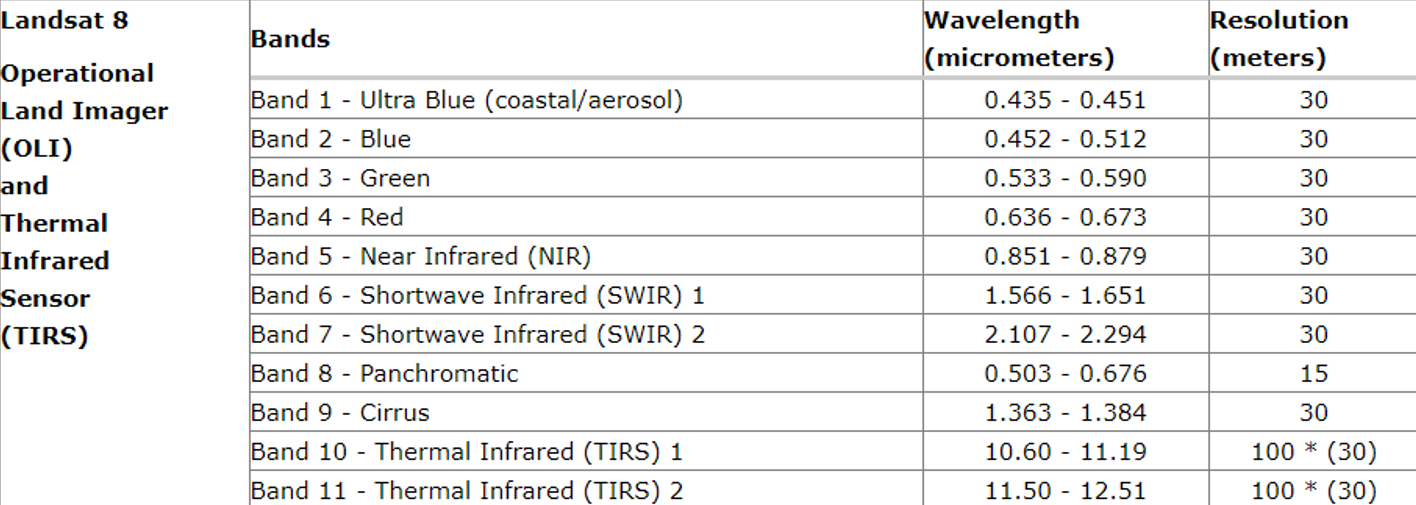
\includegraphics[width=0.7\linewidth]{figures/wavelengthL8.png}
\caption[]{Landsat 8 data specification. Source: USGS}
\end{figure}

Wavelengths of optical satellites are useful for distinguishing between forest types and other vegetation classes. Optical satellite data can be combined with laser data because the color information in optical satellite data can distinguish different vegetation types while laser data provides additional information about terrain or vegetation characteristics. 

\begin{figure}[h!]
    \begin{center}
        \begin{tabular}[b]{c}
			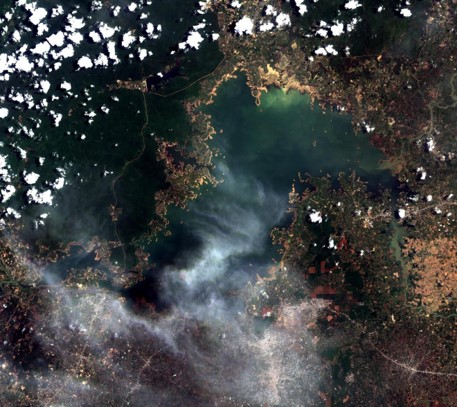
\includegraphics[width=.24\linewidth]{figures/trueColor.jpg} \\
			\small (a) True Color
          \end{tabular}
          \begin{tabular}[b]{c}
			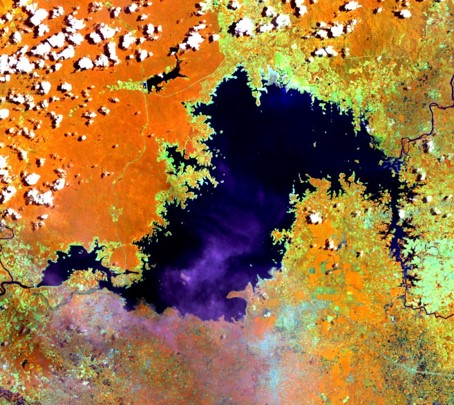
\includegraphics[width=.24\linewidth]{figures/landwater.jpg} \\
			\small (b) Land/Water
          \end{tabular}
          \begin{tabular}[b]{c}
			  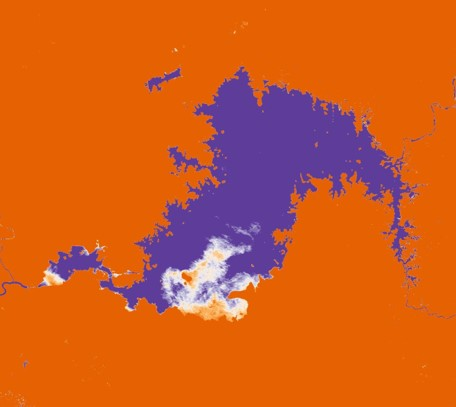
\includegraphics[width=.24\linewidth]{figures/ndwi.jpg} \\
			  \small (c) Normalized difference water index
		  \end{tabular} 
		  \begin{tabular}[b]{c}
			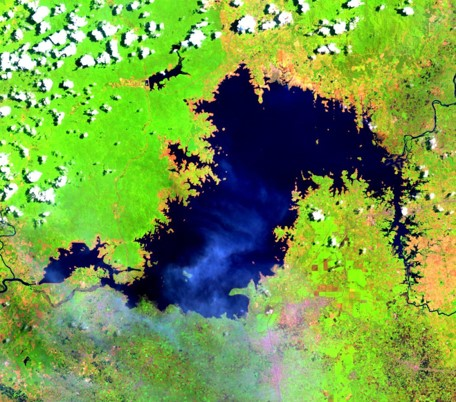
\includegraphics[width=.24\linewidth]{figures/agriculture.jpg} \\
			\small (d) Agriculture
		\end{tabular} 
    \end{center}
    \caption[]{Samples of bands combinations from Landsat 8 data files:
		\textbf{(a)} (B4, B3, B2), \textbf{(b)} (B5, B6, B4), \textbf{(c)} (B3 - B5)(B3 + B5), \textbf{(d)} (B6, B5, B2).}
\end{figure}

\subparagraph{Addition: The Landsat 8 Pre-Collection Quality Assessment (QA) band}

QA band is a part of Landsat 8 data files. Each pixel in the QA band contains integer that represent bit-packed combination of surface, atmosphere and sensor conditions that can affect overall usefulness of a given pixel. Depending on its pixel value (mostly depending on QA Bits), we can detect that pixel is a snow/ice, cloud or water (because these are mainly formed by water) or detect the cloud direction due to cirrus confidence. For more information about QA Band, see at: \href{https://landsat.usgs.gov/qualityband}{https://landsat.usgs.gov/qualityband}.

\begin{figure}
	\centering
	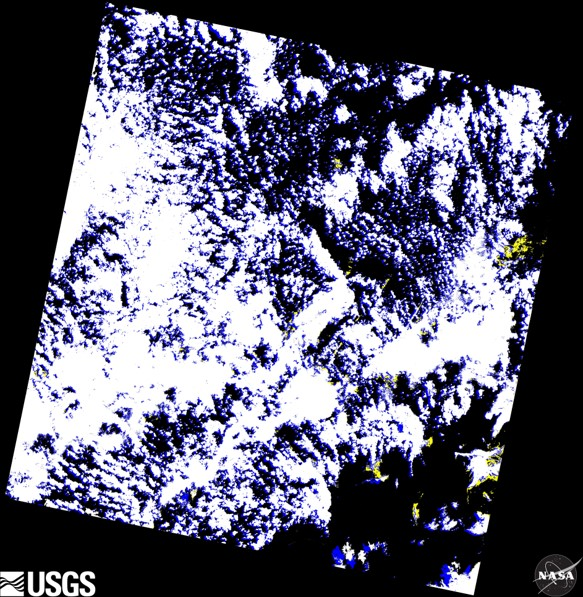
\includegraphics[width=0.32\textwidth]{figures/qaL8.jpg}
	\caption[]{Landsat 8 QA Band, Tri An Reservoir. Date taken: May 30, 2017}
\end{figure}

\subsection{Radar satellites}

Radar satellites can solve problem of satellites image on cloud days, and this is the biggest advantage of radar data over optical data. They are not affected by cloud because of its instrument specifications. For example, Sentinel-1 satellites use the C-Band Synthetic Aperture Radar (SAR). This colored Sentinel-1 SAR image is produced by showing the two polarisations (VV and VH i.e. vertical polarisation send for the radar signal and vertical or horizontal receive). 

\begin{figure}[h!]
	\centering
	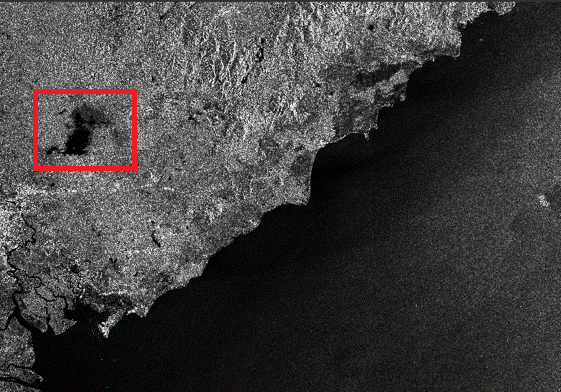
\includegraphics[width=0.6\textwidth]{figures/sarImgVVS1.png}
	\caption[]{Sentinel-1 (band VV) image, Tri An Reservoir. Date taken: June 11, 2017}
\end{figure}	

With the initial goal of monitoring reservoirs, SAR images seem to be the swiss knife to our problem until it is put in the context of machine learning the hydrological cycle of reservoirs for prediction. A long times-series of satellite images is the prerequisite to detect such patterns and therefore when it comes to SAR images the data source is very scarce. The Sentinel-1 satellites coverage is just from 2014. Other SAR image sources are costly or nontrivial to access. This makes a strong motivation for us to achieve a robust  method that remove clouds from multi-spectral satellite images and make them useful for monitoring purpose. From this point of view, a long term data source such as of Landsat-5, 7, and 8 is very useful to understand the water cycle of reservoir which is often complex by hydrological, economical, and political factors. Furthermore, multi-spectral images are useful in monitoring vegetation, which is closely related to the amount of water being used from reservoirs for irrigation. Ideally multi-spectral data can be combined with SAR data to provide the best temporal coverage and help to distinguish vegetation types while laser data provides additional information about water content in soil. 


\section{Related Work} % 2 pages

% Water Resources Monitoring problems and application. ~2 paper

Water resources monitoring provides information about the state and trend of monitored objects, which are water bodies a.k.a lakes, rivers or reservoirs on the Earth. It might be:

\begin{itemize}
	\item \textit{a local monitoring}, which can give a solution for specific local problem, on a limited part of water body or area.
	\item \textit{a global monitoring} on larger area, which has state that could be impacted or caused by some human activities.
	\item \textit{comprehensive monitoring}, which performs on a network of multi water body observation, in order to make decision for efficient use, protection and restoration of water resources.
	\item \textit{disaster monitoring}, which could immediately warn about anomaly situation on water body area, loads, etc., primarily by human activities.
\end{itemize}

Nowadays remote sensing techniques, when combines with Computing, they are used in different area of research for monitoring. For examples with internet of Things (IoT), a smart water quality monitoring system for Fuji Islands, located in the vast Pacific Ocean, is proposed in \cite{Prasad2015}. Besides that, water level monitoring and management of dams \cite{Sreekar2018} could help people on automatically closing or opening gate of the dam, depending on current water level in dams is less or higher than optimum value.

\subparagraph{Water body segmentation problems} In order to reach above aims, many different water body segmentation techniques are widely used. Each techniques could be used on some certain types. For example with multi-spectral data like Landsat, an automatic mapping water bodies approach to detect waterline boundaries is proposed in \cite{Verpoorter2012}, or applying Principle Component Analysis, which is a famous image processing technique to find out most important dimensions of data, to find out segmentation and morphology of open water bodies \cite{Jorge2006}. There are also many approaches for radar optical images. With SAR images provided by Sentinel-1, water volumes retained at reservoirs can be monitored after creating an interferometric of area \cite{Amitrano2014}, detect surface water bodies using Valley-Emphasis method \cite{Nguyen2016}.

\subparagraph{Water body recovery problems} Due to limitations of optical satellites like Landsat, MODIS, on the days that surface is covered by thick clouds, the acquired image from those devices usually suffer missing information, caused to not able to use because we can't see anything under cloudy cover. This lead to many problems on segmentation system which uses images from those satellites. In order to solve this problems, many methods have been proposed in order to recover the missing data. This kind of problem is similar to 
in-painting method in image processing field. There are variety of approaches, from using a multi-channel non-local total variation model \cite{Cheng2014}, to applying neural networks to recover\cite{Zhang2018}. Almost these method use one or more undamaged images as reference. 

\subparagraph{Prediction problems} Another problem that Machine Learning, especially Artificial Intelligence has an attractable performance is weather forecasting, a sub-prediction problem. Weather forecasting focuses mainly on the prediction of weather conditions, such as wind direction, wind speed, humidity, rainfall, temperature etc., in the given future time. In Stanford University, a temperature attribute in term of the maximum and minimum value, is being predicted in next seven days, given weather data for the past two days \cite{Holmstrom2016MachineLA}, using Regression Model. A survey of existing research on applying Artificial Neural Networks (ANNs) to weather prediction is also presented \cite{Culclasure2013UsingNN}.

\section{Contributions} % 1 pages

In this thesis, we would like to apply solutions from prediction problems, in order to solve the following things for goal of monitoring reservoirs:
    
\begin{itemize}
	\item \textit{Water body recovery problems} In order to predict a missing area in a remote sensing, we need to have at least one image called \textbf{reference image}, containing about spectral, spatial or temporal information  (the temporal information only reflects the image in another point of time in the past). Water body is mainly affected by weather and other conditions, such as water flow from other rivers to the lake, elevation and altitude of reservoir, etc. Time-series data of remote sensing provides a useful temporal information about the \textit{periodicity} or at least \textbf{trend} of water body, for example its area is increasing or decreasing, over month by month. This contribution is shown in Chapter \ref{chap-3-recover-water-body}.

	\item \textit{Monitoring water body problems} Another thing that we could analyze from predicted image is about the shape, area, volume and so on. We could compare these aspects with the same time in the past (for an example, the related month in the previous year). This leads to a very famous problem \textbf{Anomaly Detection}. This problem is also sometimes mentioned in remote sensing\cite{Grosklos2015,Yang2019}. If the techniques used in detection methods are good enough, the monitoring system will help us quickly detect strange scenarios in remote sensing time-series data. This results can be applied in many sectors such as water resource management, irrigation, and disaster prediction and prevention. The latter application is also our long-term goal where a network of interconnected reservoirs and dams  within a river basin are being monitored in order to derive from short to mid-term prediction of water level. Remote sensing imagery prediction is mentioned in Chapter \ref{chap-3-recover-water-body} and \ref{chap-4-predict-water-body}.
\end{itemize}

\section{Outlines} 

In chapter \ref{chap-1-intro}, we introduce about Remote Sensing, its problems and some state-of-the-art approaches. We also mention about our contributions and provide outlines. Chapter \ref{chap-2-dl-background} shows overview of Deep Learning, how it works and some type of Neural Networks. In next three chapters, we apply Machine Learning to solve some of Remote Sensing problems: Chapter \ref{chap-3-recover-water-body} shows recovery water body method, using trending of shape of reservoir; Chapter \ref{chap-4-predict-water-body} and \ref{chap-5-predict-from-sar-image} show how to apply machine learning on time-series data to predict next point in the sequence with the high focus on water body. Especially in chapter \ref{chap-5-predict-from-sar-image}, we also mention somethings about usage of prediction in real world problem: water body area anomaly detection, which is mainly similar to other weather forecasting problems. Finally, our thesis summaries and some of future works are mentioned in chapter \ref{chap-6-conclusions}. 

\chapter{Deep Learning Background}
\label{chap-2-dl-background}
\begin{ChapAbstract}
In this chapter, we present some background on machine learning and neural networks in general, that will make this thesis relatively self-contained. For a more thorough and slower-paced introduction we recommend the Deep learning book from Goodfellow et al \cite{dlbook}.
\end{ChapAbstract}

\section{Overview}
Machine learning is the domain of creating machines which are able to solving some specific tasks through learning from data. This is efficient in a variety of problems, consisting of time-series prediction, whose solutions are too difficult for a traditional software to deal with. However, what is exact learnt by machine in machine learning strategy? A commonly-cited definition is "A computer program is said to learn from experience \textit{E} with respect to some class of tasks \textit{T} and performance measure \textit{P}, if its performance at tasks in \textit{T}, as measured by \textit{P}, improves with experience \textit{E}" \cite{Mitchell:1997:ML}.

Deep learning uses deep neural networks to solve machine learning tasks. Neural networks include a set of neurons and connections. These neurons are managed as layers, and there are no connection between neurons in the same layer. A \textit{neuron} receives many inputs from predecessor-layer neurons and produces one output. Two special neuron's types are: inputs neurons, which are neurons in the first layer and outputs neurons, which are neurons in the last layer. A deep neural network usually has eight layers between input and output layer. Output of neuron $i$ can be transferred to input of neuron $j$, if there is a \textit{connection} between them. Each connection contains a scalar value $w$ called weight, which controls the strength of input signal by a multiplication with output of neuron $i$ before transferred to neuron $j$. Learning a neural network is finding the most appropriate weights through a process called \textit{training}.

\section{Supervised Learning}
Supervised learning is the class of learning problems where the desired output of the model on some training set is know and supplied by a supervisor. One example of this is the house's price prediction problem, where the learned model is function $\displaystyle f(x)$ that maps information of a house (area, position, architecture, prices at previous time, \dots) $\displaystyle x$ to a price in future $\displaystyle y$. In classification problem, the training set consists of a design matrix $\displaystyle X$ and a vector of scalars $\displaystyle \ry$ indicating the category of $\displaystyle X$. 

A typical supervised learning task consists of a training set $\displaystyle S$ of inputs-target pairs $\displaystyle (x, y)$, where $\displaystyle x$ is drawn from an input space $\displaystyle X$ and $\displaystyle y$ is drawn from an output space $\displaystyle Y$, and a disjoint test set $\displaystyle T \sim D = (X \times Y)$. Let consider a function $\displaystyle f : X \rightarrow Y$. The goal of supervised learning is to find $\displaystyle f$ which minimizes the error between $\displaystyle f(x)$ and $\displaystyle y$, for all $\displaystyle (x,y) \in D$, or more formally, to find $\displaystyle f$ that:
\[ f^* = \argmin_{f \in F} E_{(x,y) \sim D}[L(f(x),y)] \label{equation_all_sim_in_D}, \]
where $\displaystyle L$ is a scalar-value function representing the error of $\displaystyle f(x)$ and $\displaystyle y$. Although finding $\displaystyle f$ satisfied \eqref{equation_all_sim_in_D} is impossible (because we don't know explicitly what is $\displaystyle D$), we can switch to a simpler task by finding $\displaystyle f$, by using the i.i.d. assumption on $\displaystyle T$, such that:
\[ f^* = \argmin_{f \in F} E_{(x,y) \in T}[L(f(x), y)]\]
The i.i.d. assumption also works on the training set $\displaystyle S$, so we expect that:
\[ E_{(x,y) \in S}[L(f(x), y)] \sim E_{(x,y) \in T}[L(f(x), y)] \sim E_{(x,y) \sim D}[L(f(x),y) \]
Therefore, function $\displaystyle f$ can be found by searching over a class of functions $\displaystyle F$ whose error $\displaystyle L$ on training set $\displaystyle S$ is as small as possible:
\[ f^* = \argmin_{f \in F} E_{(x,y) \in S}[L(f(x), y)] \]
The most important and painful step in solving a supervised learning problem is to find the most appropriate class of function $\displaystyle F$, because when we already find out the structure of $\displaystyle F$, we merely focus on searching the tuple of parameters $\displaystyle \theta$ of $\displaystyle f \in F$ such that:
\[ {\theta}^{*} = \argmin_{\theta}E_{(x,y) \in S}[L(f_{\theta}(x), y)] \label{equation_loss_in_train_set_of_f_theta} \]
and totally certain that the error on test set $\displaystyle T$ is adequately small enough. There is no explicit algorithm or rule to find such $\displaystyle F$, but following some previous studies, the size of $\displaystyle f$, or $|\theta|$, is ratio with the size of training set $\displaystyle S$. Occam's Razor's principle is considerable: "If you have two equally likely solutions to a problem, choose the simplest". Therefore we should choose $\displaystyle F$ which is the simplest one among the classes of function whose size of parameter is correspondant with the size of $\displaystyle S$, in order to prevent both \textit{underfitting} and \textit{overfitting} problem.


\section{Optimization}
Optimization is included in deep learning algorithms, from supervised to unsupervised learning. In the last section, we see that we can reduce the task of learning a model for a supervised problem to solving an optimization problem of the form \eqref{equation_loss_in_train_set_of_f_theta}, where $\displaystyle \theta$ is a parameter vector and $\displaystyle E_{(x,y) \in S}[L(f_{\theta}(x), y)$ is the average loss of all examples in training set $\displaystyle S$. 

We know that it is too difficult to solve this optimization task by direct method, which is solving the system of first order differential equations. Therefore an indirect method is popularly chosen. It is called gradient descent. This method consists of two steps alternatively repeated until finding out an adequately suitable parameter $\displaystyle \theta$: the first one is evaluating $\displaystyle f(\theta)$ on the training set $\displaystyle S$ and the second is updating $\displaystyle \theta$ by taking a small steps in the negative direction of the gradient $\displaystyle \nabla_{\theta}L$. Let $\displaystyle \epsilon$ be the factor controlling the variation of $\displaystyle \theta$ in each iteration, which is called \textit{learning rate}. These two steps can be represented by algorithm \ref{alg:GD}:
\begin{algorithm}
    \caption{Gradient Descent} \label{alg:GD}
    \begin{algorithmic}[1]
        \State $\theta_0 \gets \textit{Initialize}$
        \For{\texttt{iterations}}:
            \State $\theta_{t + 1} \gets \theta_{t} - \nabla F(\theta_{t}) . \epsilon$
            \State $t \gets t + 1$
        \EndFor
    \end{algorithmic}
\end{algorithm}

However, gradient descent method has some disadvantages that make it hard to be applied in reality. The first is that it highly depends on initialization and leads to a stuck in local optima. The second is that it need a careful selection of learning rate. Time to wait for one update is correlated with the number of examples in training set, which may be more than millions, so if the parameter $\displaystyle \theta$ is not updated in a right way, we need to restart the training process and waste a lot of useless time.

In order to improve gradient descent, many gradient-based methods are invented, such as Stochastic Gradient Descent (SGD) \cite{SGD}, Momentum \cite{Momentum}, Adadelta \cite{DBLP:adadelta}, Adam \cite{article:Adam-optimization}, \dots. In SGD, we only take a small minibatch of training examples, at a time and update parameter $\displaystyle \theta$ using these examples, which is suitable for our hardware resources. The pseudo code of SGD is summarized in the following algorithm \ref{alg:SGD}.
\begin{algorithm}
    \caption{Stochastic Gradient Descent} \label{alg:SGD}
    \begin{algorithmic}[1]
        \State $\theta_0 \gets \textit{Initialize}$
        \Repeat
            \State Sample a minibatch of $\displaystyle m$ of examples $\displaystyle \{(x_1, y_1), \dots, (x_m, y_m)\}$ of $\displaystyle S$
            \State Estimate the gradient $\displaystyle \nabla_{\theta}F(\theta) \approx \nabla_{\theta}[\frac{1}{m}\sum_{m}^{1}{L(F(x_i, \theta),y_i)}]$ with backpropagation
            \State Perform a parameter update: $\displaystyle \theta \gets \theta - \epsilon . \nabla_{\theta}F(\theta)$
        \Until{convergence}
    \end{algorithmic}
\end{algorithm}

However, convergence rate of SGD on large datasets may be slow. Today, the most cited optimization algorithm is Adam \cite{article:Adam-optimization}. It is also one of optimization algorithms used in this work. For more information on optimization strategies, see chapter 8 \cite{dlbook}.

\section{Backpropagation}
We saw that if we can evaluate the gradient of the loss function then we can use stochastic gradient descent to minimize it, and in the process find mappings $\displaystyle f \Rightarrow F$ that achieve low cost and map $\displaystyle X$ to $\displaystyle Y$ consistent with the training data.

We now discuss backpropagation - the process by which we eciently compute gradients of scalar valued functions with respect to their inputs. The backpropagation algorithm is a recursive application of the chain rule from calculus. Recall that the function we are interested in computing gradients of is $\displaystyle g$, which takes as input the dataset of examples $\displaystyle (x_i, y_i)$ and the parameters $\displaystyle \theta$. We are specifically interested in the gradient $\displaystyle \nabla_\theta g$ with respect to the parameters $\theta$ in order to perform the parameter update but we could, if we wanted to, also compute the gradients for the inputs $\displaystyle x_i$ with the same process.

More formally, suppose we had an input vector $\displaystyle x_0$ that we transform through a series of functions $\displaystyle x_i = f_i(x_{i-1})$ where $i = 1,\dots,k$ and the last $\displaystyle x_k$ is a scalar. We assume that the gradient exists, so we can calculate the Jacobian matrix $\displaystyle \frac{\partial x_i}{\partial x_{i-1}}$ of all intermediate transformations, which tells us how every output dimension of $\displaystyle x_i$ depends on every input dimension of $\displaystyle x_{i-1}$. By chain rule, the final gradient we are interested in is simply the matrix product of all the Jacobians: $\displaystyle \frac{\partial x_k}{\partial x_0} = \prod_{i=1}^k \frac{\partial x_i}{\partial x_{i-1}}$.

In neural network applications we first perform a \textit{forward pass} in which we take a batch of data $\displaystyle (x_i, y_i)_{i=1}^m$ and current parameters $\displaystyle \theta$ and “forward” the network to compute all intermediate values (caching them for later) and the cost $\displaystyle g$.  Then during backpropagation we proceed backwards through all intermediate stages (the “backwards pass”) and “chain” the local gradients, each time matrix multiplying by the next Jacobian matrix in the full product. In many cases we do not need to actually create the full Jacobian matrices and can take advantage of special structure to chain the gradients in a more computationally ecient manner.

Today, most implementations of backpropagation organize the code base around a \textit{Graph} object that maintains the connectivity of operations (also called gates, or layers) and a large collection of possible operations. Both Graph and Node objects implement two functions: \texttt{forward()} and \texttt{backward()}. The Graph’s \texttt{forward()} iterates over all nodes in the topological order and calls their \texttt{forward()}, and its \texttt{backward()} iterates in the reverse order and calls their \texttt{backward()}. Each Node computes its output with some function during its \texttt{forward()} call, and in \texttt{backward()} it is given the gradient of the loss function with respect to its output and returns the “chained” gradients on all of its inputs. By “chained” we mean taking the gradient on its output and multiplying it by its own local gradient (the Jacobian of this transformation). This gradient then flows to its children nodes that perform the same operation recursively. As a last technical note, if the output of a node is used in multiple places in the graph then correct behavior by the multivariable chain rule is to add the gradients during backpropagation along all branches. This would be handled in the Graph object.

\section{Neural Networks}
\subsection{Feedforward Neural Networks}
The Feedforward Neural Network ($\displaystyle FNN$) is the most basic type of neural networks. A $\displaystyle FNN$ consists of a number of layers of artificial neurons which represent how input data are transformed to produce desired output. This type of network is called \textbf{Feedforward} because it may be considered as a flow from input $\displaystyle x$, through some intermediate computations, and finally to output $\displaystyle y$. The information is transfered in only one way, from layer $\displaystyle i$ to layer $\displaystyle i + 1$, without feedback from deeper layers to the previous layers. A layer is typically the composition of these operations: matrix multiplication and activation function. For example, a 2-layer $\displaystyle FNN$ can be formulated as $\displaystyle y = W_2(\sigma(W_1(x)))$, $\displaystyle W_1, W_2$ are real-number matrices and $\displaystyle \sigma$ is a non-linear activation function, such as $\displaystyle tanh$, $\displaystyle sigmoid$, $\displaystyle relu$.

Formally, a Feedforward Neural Network with $\displaystyle l$ hidden layers (layers between input and output layer) can be parameterized by $\displaystyle l + 1$ weight matrices $\displaystyle (W_0, W_1, \dots, W_l)$, $\displaystyle l + 1$ scalar bias $\displaystyle (b_0, b_1, \dots, b_l)$ and $\displaystyle l$ activation functions $\displaystyle \sigma_1, \dots, \sigma_l$. Let $\displaystyle x$ is input, the feedforward neural networks is computed as algorithm \ref{alg:FNN}:
\begin{algorithm}
    \caption{Feedforward Neural Network} \label{alg:FNN}
    \begin{algorithmic}[1]
        \State $z_0 \gets x$
        \For{i \textbf{from} $1$ \textbf{to} $l + 1$}
            \State $x_i \gets W_{i - 1}z_{i - 1} + b_i$
            \State $z_i \gets \sigma_i(x_i)$
        \EndFor
    \end{algorithmic}
\end{algorithm}

A typical example of $\displaystyle FNN$ is the $\displaystyle XOR$ problem. $\displaystyle XOR$ function is the operation of two binary values, $\displaystyle x_1$ and $\displaystyle x_2$. The result of $\displaystyle XOR$ function is $\displaystyle 1$ if $\displaystyle x_1$ and $\displaystyle x_2$ are equal, and is $\displaystyle 0$ otherwise. To solve this problem by neural networks, we first consider a single-layer perceptron ($\displaystyle y = \sigma(W_1x + b_1)$). After a time of trying to fit this network, we get a stuck that the this single-layer network can only approximate linearly separable functions. However, $\displaystyle XOR$ function isn't linearly separable (see figure \ref{fig:xor}).
\begin{SCfigure}
    \caption{An illustration of $\displaystyle XOR$ problem. We see that we cannot separate the same color points by only one line.}
    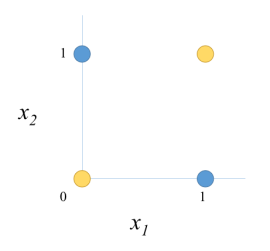
\includegraphics[width=.4\textwidth]{figures/chap2/xor-graph.png}
    \label{fig:xor}
\end{SCfigure}

Now let consider a 1-hidden-layer $\displaystyle FNN$ with activation function relu ($\displaystyle relu(x) = max(0, x)$), we can now specify $\displaystyle XOR$ function as:
\[ f(x; W_1, W_2, b_1, b_2) = W_2.max(0, W_1x + b_1) + b_2 \label{equation_xor} \]
We can now specify a solution to the $\displaystyle XOR$ problem. Let
\[ W_1 = 
\begin{bmatrix}
    1 & 1 \\
    1 & 1
\end{bmatrix}, \]

\[ b_1 =
\begin{bmatrix}
    0 \\
    -1
\end{bmatrix}, \]

\[ W_2 =
\begin{bmatrix}
    1 & -2
\end{bmatrix}, \]

and $\displaystyle b_2 = 0$. We can check the result by computing the value of \eqref{equation_xor} with the given input $\displaystyle X$ below:
\[ X = 
\begin{bmatrix}
    0 & 0 & 1 & 1 \\
    0 & 1 & 0 & 1
\end{bmatrix}, \]
where each column of $\displaystyle X$ is an input pair $\displaystyle (x_1, x_2)$,
\begin{align*}
    f(X; W_1, W_2, b_1, b_2) &= W_2.max(0, W_1x + b_1) + b_2 \\
    {} &= \begin{bmatrix}
            1 & -2
          \end{bmatrix}.max \left(0, 
            \begin{bmatrix}
                1 & 1 \\
                1 & 1
            \end{bmatrix} \begin{bmatrix}
                0 & 0 & 1 & 1 \\
                0 & 1 & 0 & 1
            \end{bmatrix} + \begin{bmatrix}
                0 \\
                -1
            \end{bmatrix}\right) + 0 \\
    {} &= \begin{bmatrix}
        1 & -2
      \end{bmatrix}.max \left(0, 
        \begin{bmatrix}
            0 & 1 & 1 & 2 \\
            0 & 1 & 1 & 2
        \end{bmatrix} + \begin{bmatrix}
            0 \\
            -1
        \end{bmatrix}\right) \\
    {} &= \begin{bmatrix}
        1 & -2
        \end{bmatrix}.max \left(0, 
        \begin{bmatrix}
            0 & 1 & 1 & 2 \\
            -1 & 0 & 0 & 1
        \end{bmatrix}\right) \\
    {} &= \begin{bmatrix}
        1 & -2
        \end{bmatrix}.\begin{bmatrix}
            0 & 1 & 1 & 2 \\
            0 & 0 & 0 & 1
        \end{bmatrix}\\
    {} &= \begin{bmatrix}
        0 & 1 & 1 & 0
        \end{bmatrix}
\end{align*}
We can see that the final result is exactly what we expected.


\subsection{Convolutional Neural Networks}
Convolutional Neural Networks (CNNs) are a specialized kind of feedforward neural networks for processing data that has a grid-like topology. This type of networks archives a considerable amount of success in many machine learning problem, from 1D data (time-series audio signal, etc) to 2D data (computer vision, etc). The most noticeable difference between CNNs and FNNs is that instead of using a matrix multiplication as FNN, CNNs use convolution operation. In the context of this thesis, we concentrate on the 2D convolution operation executed by two operators: a matrix which is the restricted portion of the receptive field and a matrix which is the set of learnable parameters (a.k.a. kernel). The kernel is spatially smaller than an image, but has the same number of channels. For example, if the image is composed of three (RGB) channels, the kernel height and width will be spatially small, but the depth extends up to all three channels. Usually, there is more than one kernel in the same convolutional layer, e.g. 16, 32, 64 kernels.

\textbf{Concrete Example.} Suppose that we have a input image $\displaystyle X$ with size \newline $\displaystyle 32 \times 32 \times 3$, a kernel $\displaystyle w$ with size $\displaystyle 5 \times 5 \times 3$, padding isn't used and stride is $1$. This kernel has $\displaystyle 5 * 5 * 3 = 75$ parameters to be learnt. We can convolve this filter by sliding it across all spatial positions of the input tensor and computing a dot product between a small chunk of $\displaystyle X$ and the filter $\displaystyle w$ at each position. The result will be an activation map, which in this case would have the dimensions $\displaystyle 28 \times 28$ (28 is the number of unique positions that a filter of 5 elements can be placed over an input of size 32) (An example of convolution operation is in figure \ref{fig:cnn}). In some cases, padding is used when users want to increase the spacial dimensions of the output (commonly the same as input tensor $\displaystyle X$). In addition, if there is no padding and stride 2 is used, output tensor has size of $\displaystyle 14 \times 14$. Finally, if kernel size is set to 64, input tensor $\displaystyle X$ executes convolution operation independently with these filters, and the final output has the shape of $\displaystyle 28 \times 28 \times 64$.

\begin{figure}[h!]
    \begin{center}
        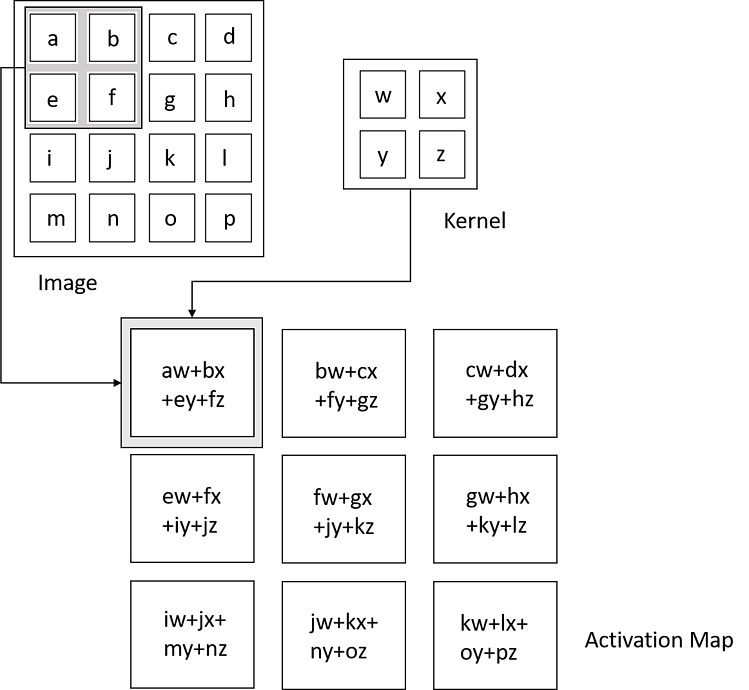
\includegraphics[width=0.7\textwidth]{figures/chap2/cnn.png}
        \caption{Convolution Operation \cite{dlbook}}
        \label{fig:cnn}
    \end{center}
\end{figure}

\textbf{General definition.} Formally, a convolutional layer for images (assuming input tensors with three spatial dimensions):
\begin{itemize}
    \item Has a $\displaystyle W_1 \times H_1 \times D_1$ tensor as input.
    \item Requires \textbf{4 hyperparameters}: The number of filter $\displaystyle K$, the spatial dimension $\displaystyle F$, the stride $\displaystyle S$, and the amount of padding on the borders of the input, $\displaystyle P$.
    \item The number of parameters of each filter is $\displaystyle F \times F \times D_1$ and one bias (if used bias), so with a set of $\displaystyle K$ filters, there is totally $\displaystyle K \times F \times F \times D_1$ weights and $\displaystyle K$ biases.
    \item The output is a tensor of size $\displaystyle W_2 \times H_2 \times K$, where $\displaystyle W_2 = (W_1 - F + 2P)/S + 1$, $\displaystyle H_2 = (H_1 - F + 2P)/S + 1$.
\end{itemize}

\section{Recurrent Neural Networks}
In this section, we introduce briefly Recurrent Neural Networks (RNNs), which is the type of neural networks mainly used in this work. RNNs show their significant performance in many problems where input data are in form of sequence, such as language model or time-series predictions. The original idea of RNNs comes from the sharing parameter mechanism, which is presented in CNNs. However, while CNNs is only capable of sharing parameter across a small number of neighbors, RNNs allow to share parameters through further neigbors, maybe hundred-length sequences.  

\subsection{Vanilla Recurrent Neural Networks}
Vanilla Recurrent Neural Network is the most basic and natural method when humans first think about applying recurrent mechanism in neural networks. In a Vanilla RNN, each output at index $\displaystyle t$ is a function of the output at index $\displaystyle t - 1$, except output at index $\displaystyle 0$ (it is usually zero-initialized or also learnable parameters). The typical function in RNN is:
\[ h_t = \tanh \left( W\begin{pmatrix} x_t \\ h_{t-1} \end{pmatrix} \right) \]

However, Vanilla RNNs have low performance on long sequence data, due to \textit{vanishing} and \textit{exploiding} gradient. Exploiding gradient, which means that gradient's value becomes too large through recurrent backpropagation (due to multiple multiplication with many greater-than-1 numbers), is rarely occured, but its consequence is also huge. Clipping gradient \cite{DBLP:Clipping-gradient} is an efficient solution for this problem. However, vanishing gradient can't be solved by this method. Vanishing gradient happens when a gradient is multipled by many \textit{absolutely-smaller-than-1} numbers and reaches zero, which leads to the reduction of the weight correspondant to this gradient.

\subsection{Long-Short Term Memory Neural Networks}
There are a number of variants of LSTM. In this work, we use the LSTM with "peephole connections" of Gers and Schmihuber (2000) \cite{Peephole-LSTM}, which makes use of information at the previous cell state to be a part of input of gate layers. The formula of LSTM is described by equations \eqref{equation-lstm-ft} to \eqref{equation-lstm-ht}

\[ f_t = \sigma(W_f[C_{t-1}, h_{t-1},x_t] + b_f) \label{equation-lstm-ft}\] 
\[ i_t = \sigma(W_i[C_{t-1}, h_{t-1},x_t] + b_i) \label{equation-lstm-it}\]
\[ \hat{C}_t = \tanh(W_c[C_{t-1}, h_{t-1},x_t]) \label{equation-lstm-Chat-t}\]
\[ C_t = f_t * C_{t-1} + i_t * \hat{C}_t \label{equation-lstm-Ct}\]
\[ o_t = \sigma(W_o[C_{t}, h_{t-1},x_t] + b_o) \label{equation-lstm-ot}\]
\[ h_t = o_t * \tanh(C_t) {equation-lstm-ht}\]


\section{Summary}
In summary, a typical workflow for applying a neural network in some context looks as follows:

\textbf{Data preparation.} First, obtain a dataset. For the purposes of this dissertation we have assumed that the dataset is made up of a set of pairs $\displaystyle (x, y)$ where $\displaystyle x$ is some input example and $\displaystyle y$ is a label. We then split the dataset into three folds, commonly a training, validation and test fold (common proportions could be 80\%, 10\%, 10\% respectively). We will use the training fold for optimizing the parameters with backpropagation, the validation fold for hyperparameter optimization, and the test fold for evaluation (discussed below in more detail).

\textbf{Data preprocessing.} Preprocessing the data can help improve convergence of neural networks. For images, common preprocessing techniques involve standardizing the data (subtracting the mean and dividing by the standard deviation individually for every input dimension of $\displaystyle x$), or at the very least subtracting the mean. It is critical to estimate these statistics only on the training data, and using these fixed statistics to process the validation and test data, as this appropriately simulates the deployment of the final system into a real-world application.

\textbf{Architecture design.} Next we must to decide on a family of architectures that we wish to explore. In our notation above, this amounts to designing the internals of the computation graph that makes up the function $\displaystyle f$. This stage is more of an art than a science, but we discuss a few common heuristics used in practice. It is common to process pixel data with convolutions and sequence data with recurrent networks. For the scale of the architecture, a very rough rule of thumb is that the full model should have approximately similar number of parameters as there are examples in the training dataset.

\textbf{Optimization.} A default recommendation is to use Adam \cite{article:Adam-optimization} for optimization, with learning rates of approximately $\displaystyle 1e3$, the coecient of first moment of $\displaystyle 0.9$ and second moment $\displaystyle 0.99$. It is often beneficial to anneal the learning rate during the course of training by approximately a factor of $\displaystyle 100$ by the very end of training, but it si common to decay the first time only after half of the training is finished. As a a good sanity check to help debug the code, it is a good idea to try to
overfit a single batch of data (reaching zero training loss) before optimizing over the full training set.

\textbf{Hyperparameter optimization.} The optimization with stochastic gradient can be seen as an inner loop of the optimization, while hyperparameter optimization is the outer loop that determines good values of hyperparameters that are dicult or impossible to backpropagate into (such as the learning rate, or the number of units in the hidden layers). This process consists of sampling hyperparameters from some search range (it is best to sample at random rather than along the grid), optimizing the model, and evaluating the model on the validation fold. The final best model is the one that achieves the best validation performance.

\textbf{Evaluation.} Once we identify the best trained model (with the lowest validation loss), we evaluate the model a single time on the test set and report the performance. Consistent improvements can always be obtained by using model ensembles, which average the results of evaluating multiple models trained from different initializations or with dfferent hyperparameters.

\chapter{Recover Water Body from Cloud Covered Optical Satellite Images}
\label{chap-3-recover-water-body}
\begin{ChapAbstract}

In this chapter, we would like to apply information about trending of monitored objects, which are water bodies like lakes or reservoirs, which has periodical information about volume, flow or area. As we've known, water body is mostly affected by weather and other conditions, such as water flow from other rivers to the lake, elevation and altitude of reservoir, etc. Time-series of data may provide the \textbf{trend} of water body, for example its area is increasing or decreasing, it usually has a large or small area of water body in some months. This might lead to higher accuracy when using as reference in recovery problems. So that, in this chaper, we will try to apply a periodicity of weather into remote sensing in-painting problems.

\end{ChapAbstract}

\section{Related Work}

Different from other image types, remote sensing imagery has many useful attributes for recovery process, including spatial, spectral and temporal information. Depending on those information, many missing information recovery methods for remote sensing imagery has been proposed, which can be classified into four main categories: 

\begin{enumerate}
	\item \textbf{Spatial-based methods}\cite{Zhang2006,YangLLSWL16}. This method is also known as \textit{inpainting} method. These are the most basic method in image reconstruction, assume that undamaged regions have the same or related statistical features or texture information as the missing regions. These methods are suitable for recovering the small areas or regions, so that are not qualified for reconstructing for large or complex area such as remote sensing.
	
	\item \textbf{Spectral-based methods}\cite{Lingli2006,Li2014}. Because optical satellites data provides multiple bands data, so that these methods usually use a spatial correlation between different bands to reconstruct missing data. These methods are mostly taken experiments on Terra MODIS band 6, because this band is often damaged, and band 6 and 7 are closely correlated. Because these methods have a high level of accuracy, it also can't deal with thick cloudy cover, because in this situation, all bands are affected due to limitation of optical satellites.
	
	\item \textbf{Temporal-based methods}\cite{ZENG2013182,Gao2017}. Temporal information can be used to recover missing data. The main idea is using the remote sensing data in the same region, but different times. Some use only one, others use many images. In summary, these methods work well for a variety of situations, including thick clouds, but it mainly \textit{selects the most similar regions to recover missing region}.
	
	\item \textbf{Hybrid methods}\cite{Ng2017,Li2016}. These methods are merged from some of above methods, which could take advantages of each method, in order to produce higher accuracy. 
\end{enumerate}

Most of above methods only aims to take some example looks under cloud cover, so the common thing between above methods is only using one or two images related to damaged image as reference. From deep learning based method, Unified Spatial-Temporal-Spectral Deep Convolutional Neural Network (STS-CNN), in removing clouds using multi-spectral images from single band \cite{Zhang2018}, we propose new neural network architectures that make use of temporal series of multi-spectral images to recover better cloud-free images. Notice that, \textit{\textbf{STS-CNN} only feeds one image as referenced image and \textit{temporal} just means \textit{at different times}, not use periodicity attribute of weather.}

\begin{figure}[h!]
%	\centering
	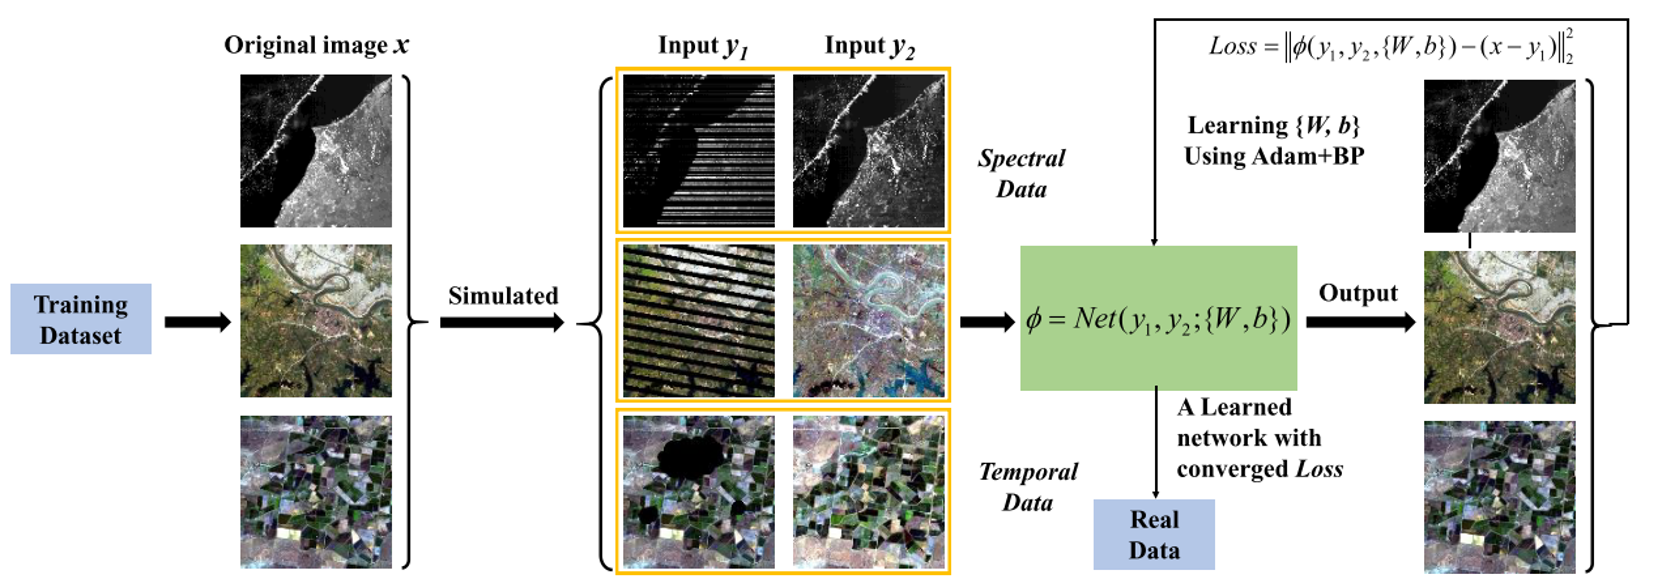
\includegraphics[width=1\textwidth]{figures/sts-cnn_framework.png}
	\caption{Flowchart of the STS-CNN framework in \cite{Zhang2018}}
\end{figure}

\section {Dataset}
In this chapter, Tri An reservoir is chosen for experiments, because it has enough large area for visualization, segmentation and calculation. Each tile from satellite imagery can only focus on part of the Earth, and Tri An reservoirs' water body belongs to one tile, so that it is not necessary to concatenate many tiles.

\begin{figure}[h!]
	\centering
	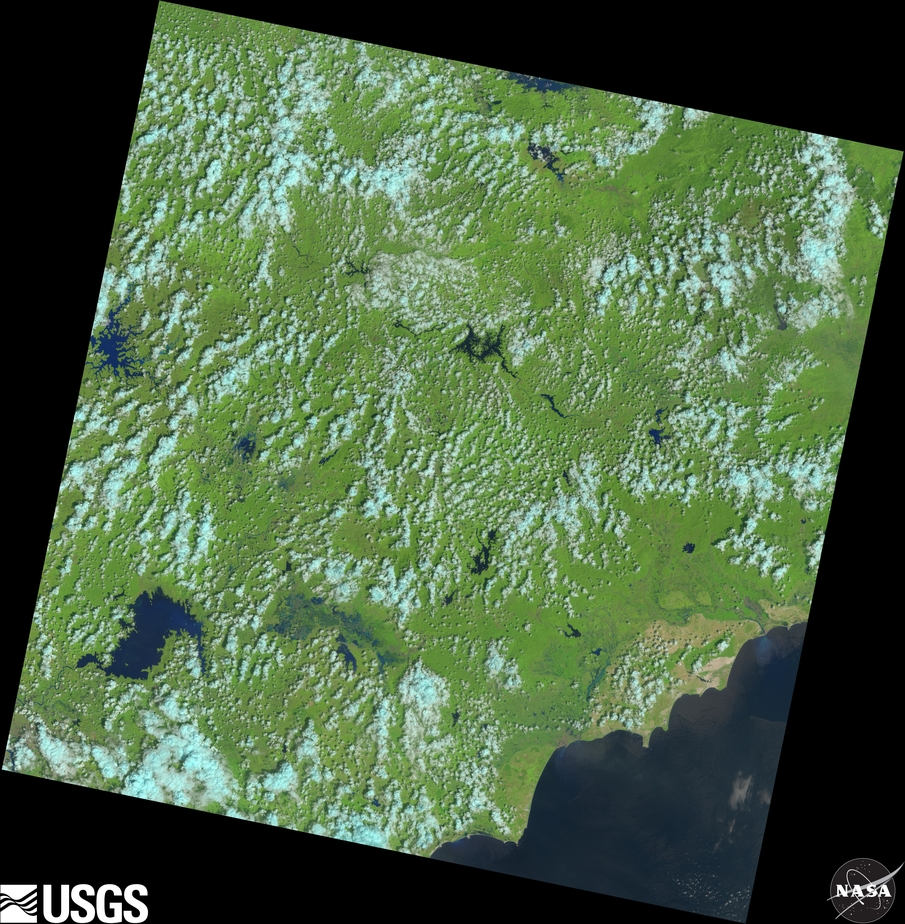
\includegraphics[width=0.4\textwidth]{figures/l8tile.png}
	\caption{Tri An Reservoir belongs to a tile of Landsat 8 data file, taken on January 10, 2013}
\end{figure}	


We use Landsat 8 data for optical satellite. For radar satellite, Sentinel-1 images are chosen. Those data can be freely acquired from the Internet.

\subparagraph{Requiring time period} \textbf{Landsat 8} data files are collected in period November 2013 - May 2018. SAR Imagery from \textbf{Sentinel-1} are from April 2014 - May 2018.

\section{Model}

In this method, we will refer a neural network of STS-CNN\cite{Zhang2018} to re-implement a neural network to our data. 

This algorithm has 3 inputs: (1) A missing image, (2) a referenced image and a missing image (1) with damaged regions filled by corresponding region in referenced image. The output is a recovered image. Note that, we have three images as input, and the third aims to tell a neural network easier to determine which are missing regions on the images. The referenced image will be also taken from Landsat 8, on cloudy-free day. For equal comparison to original method, we will use example of masks that provided with this paper, can be found at: \href{https://github.com/WHUQZhang/STS-CNN/}{https://github.com/WHUQZhang/STS-CNN/}.

The optimizer function is $Adam$ and the learning rate of whole network is $1e-4$. Model at figure \ref{fig:modifiedModel} contains 3 inputs: \textit{Input 1}: damaged image, \textit{Input 2}: referenced image and \textit{Input 3}: referenced with simulated-missing regions like \textit{Input 1}.

\begin{figure}[h!]
	\centering
	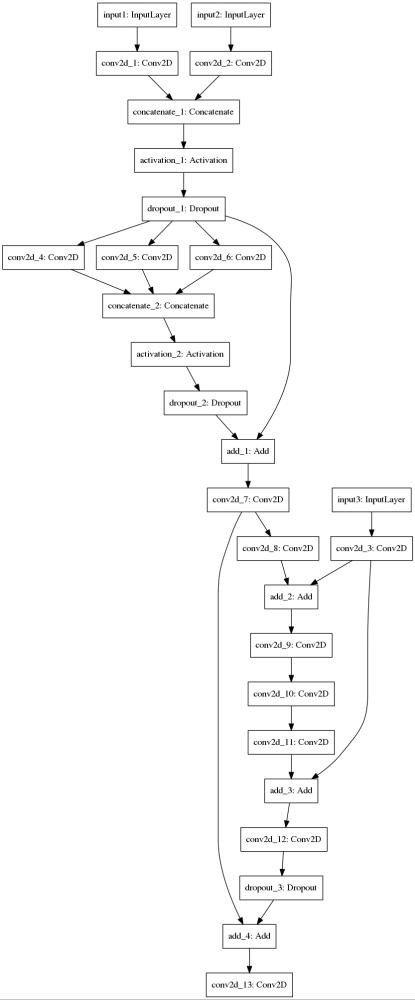
\includegraphics[width=0.6\textwidth]{figures/modifiedModel.png}
	\caption{Modified model from STS-CNN.}
	\label{fig:modifiedModel}
\end{figure}	

For comparison, we will use cloud-free image and add on it two type mask to feed into network. The first type is a simple shape mask from original method. The second is get from QA Bands of one cloud day, which is acquired by Landsat 8. In order to get cloud cover, F-mask program (Python, \href{http://pythonfmask.org}{http://pythonfmask.org}) is used to get cloud mask from QA Bands. The table shows difference between original method and my re-implemented method. For more visualization, take a look at figure \ref{fig:improvedModel_experiment_1}, \ref{fig:improvedModel_experiment_2} and \ref{fig:improvedModel_experiment_3} in \ref{experiment_improvedModel}. For measuring between methods, in this chapter, we use Peak signal-to-noise ratio.

\subparagraph{Peak signal-to-noise ratio} \textit{Wikipedia} It often abbreviated $PSNR$, is an engineering term for the ratio between the maximum possible power of a signal and the power of corrupting noise that affects the fidelity of its representation. Because many signals have a very wide dynamic range, $PSNR$ is usually expressed in terms of the logarithmic decibel scale. 

\begin{equation}
\label{psnr_eq}
\centering
PSNR \textrm{ = } 20 * log_{10}(MAX_I) - 10 * log_{10}(MSE)
\end{equation}

where $MAX_I$ is the maximum possible value of image $I$, depending on its depth. For example, if the pixels are represented using 8 bits per sample ($8-bit$ image), this is 255. More generally, when samples are represented using linear PCM with $B$ bits per sample, $MAX_I$ is $2^B$ $-$ $1$. \textit{Mean square error}, $MSE$, between the original image $I$ with predicted image $K$, with the same of size ($m, n$) will be calculated as following:

\begin{equation}
\centering
MSE \textrm{ = } \frac{1}{mn} \sum_{i \textrm{ = } 1}^{m} \sum_{j \textrm{ = } 1}^{n} [I_{i,j} - K_{i,j}]^2
\end{equation}

\vspace{0.3cm}
Here is table of comparison. Pixel value are scale to $(0..1)$ and $(0..255)$ (original has pixel range from $0..65535$). All are calculated by $PSNR$ (higher is better).

\begin{table}[h!]
	\centering
	\begin{tabularx}{\textwidth}{|c|c|c|c|}
		\hline
		& STS-CNN & Modified model (0..1) & Modified model (0..255) \\ \hline
		Simple cloud         & 19.9098 & \textbf{27.00188}                                                & 26.7391                                                            \\ \hline
		Simple multi-cloud   & 15.6941 & \textbf{23.8445}                                                 & 23.80995                                                           \\ \hline
		Real (complex) cloud & 12.8381 & \textbf{19.70776}                                                & 19.5976                                                            \\ \hline
	\end{tabularx}
	\caption{Comparison between proposed model to modified model}
\end{table}

\section{Optimization}

As periodicity of weather is being used for higher accuracy in recovering water body, we use two methods below on our dataset: (1) \textbf{Using Time-Distributed Layer from Keras}; (2) \textbf{Recurrent-CNN}, which uses a kind of Recurrent Neural Network, Long-Short Term Memory. A common thing between between two approaches is applying a temporal slice of images into neural network, and the purpose of those sub-networks is predicting the next images to be referenced image. 

\subsection{Using Time-Distributed Layer from Keras}

Keras framework also provides Time-Distributed layers, which applies for every temporal slice of an input. Because of limitation of hardware memory, we feed into it five consecutive images acquired from Landsat 8. For referenced image, we try with 2 type: first is Landsat 8 and the second is Sentinel-1. Because only water body is focused, so we've classified water body on Sentinel-1 data, and resize it to the same of Landsat 8 (Sentinel-1 has 10 meters of resolution). Model specification contains 2 part: \textit{part 1}  (at Fig. \ref{fig:timemodelPart1}) is about using Time-Distributed to get predicted image as reference, \textit{part 2} (at Fig. \ref{fig:timemodelPart2}) is quite similar to existing method for reconstruction.

\begin{figure}[h!]
	\centering
	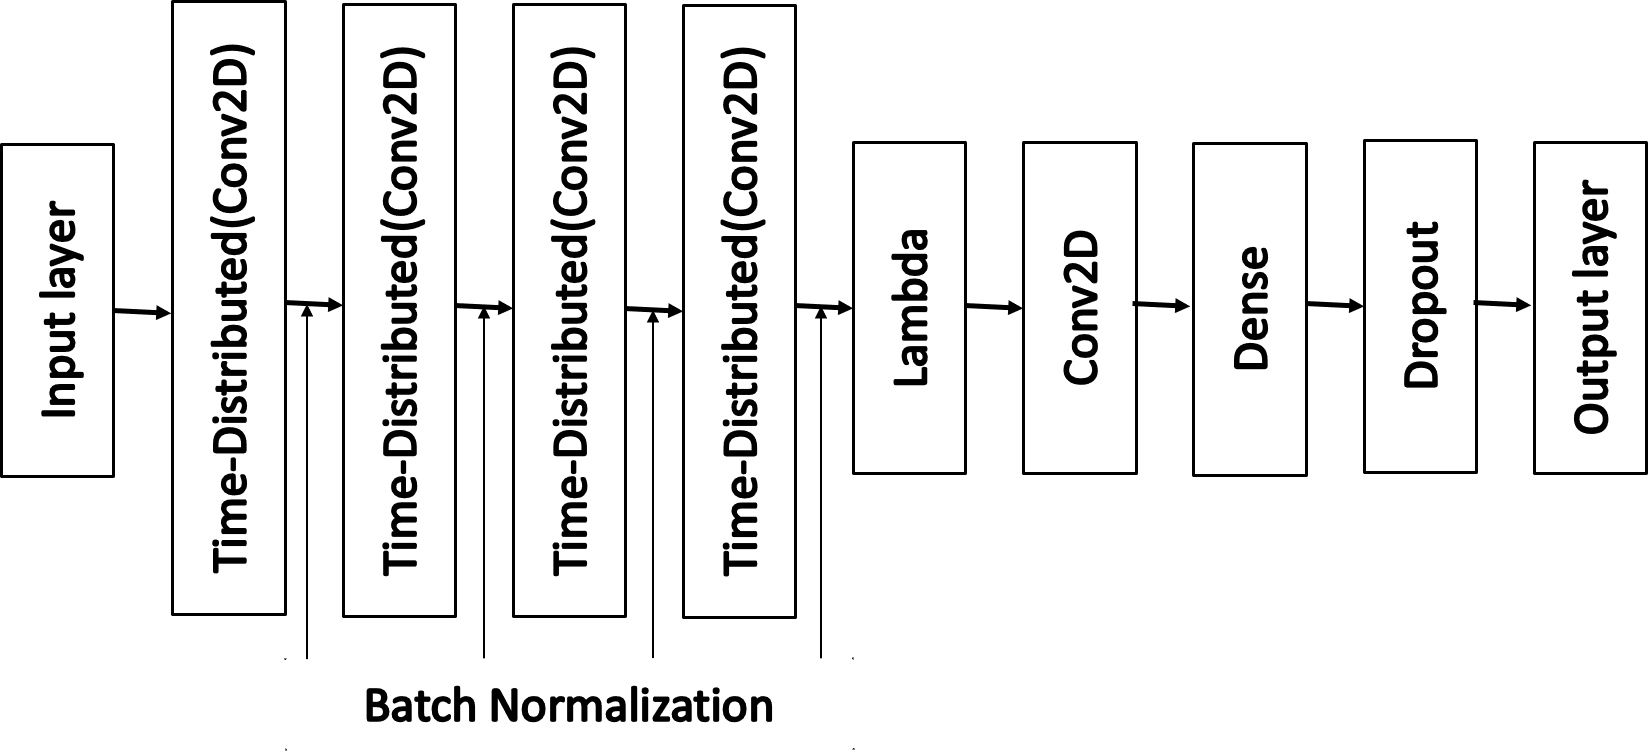
\includegraphics[width=0.5\textwidth]{figures/timemodelPart1.png}
	\caption{Applying Time-Distributed in Neural Network. Lambda is a function to get 1-time next predicted image from time-series images to be reference image.}
	\label{fig:timemodelPart1}
\end{figure}

\begin{figure}[h!]
	\centering
	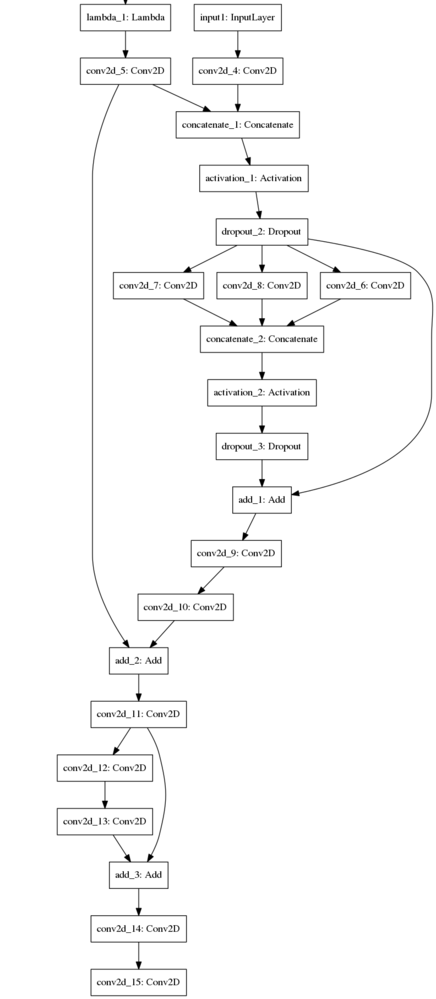
\includegraphics[width=0.7\textwidth]{figures/timemodelPart2.png}
	\caption{Using predicted image as reference image, with part in order to reconstruct missing regions. Note that there is not input \textit{referenced image with missing data}}
	\label{fig:timemodelPart2}
\end{figure}

\subsection{Recurrent-CNN implementation}

The idea behind Recurrent Neural Networks (RNNs) is to make use of sequential information. So that, this approach aims to use Long Short Term Memory networks – usually just called “LSTMs” – are a special kind of RNN, capable of learning long-term dependencies, to make prediction of next image, based on five consecutive images, and use the next image as referenced image for reconstruction. For the predictive part, see \ref{fig:modelConv2DLSTM_1}. The main is similar to \ref{fig:timemodelPart2}

\begin{figure}[h!]
	\centering
	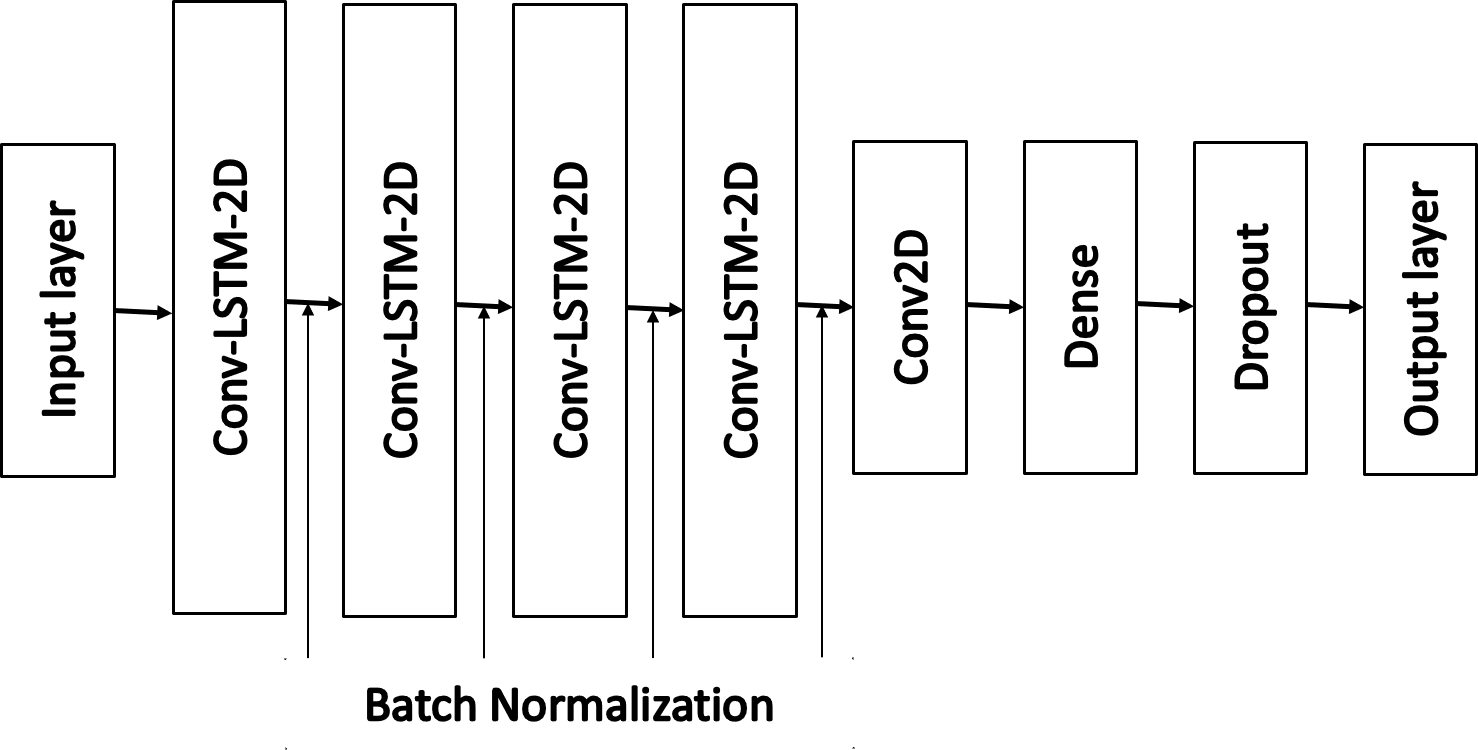
\includegraphics[width=0.5\textwidth]{figures/modelConv2DLSTM_1.png}
	\caption{LSTM (as Conv2DLSTM Layer) aims to predict the next image to be used as referenced image}
	\label{fig:modelConv2DLSTM_1}
\end{figure}

\subsection{Comparison}

This is a comparison between above methods. Visualization is available at \ref{experiment_timeSeriesModel}, in which \textit{Input 1 is damaged image, input 2 is a time-series data (5 images)}. 

\begin{table}[h!]
	\centering
	\begin{tabularx}{\textwidth}{|c|c|c|}
		\hline
		& Time-Distributed Layer & LSTM-Conv2D \\ \hline
		Simple cloud         & \textbf{30.5584}                                                  & 23.4441     \\ \hline
		Simple multi-cloud   & \textbf{29.9230}                                                  & 24.0554     \\ \hline
		Real (complex) cloud & \textbf{30.4467}                                                  & 26.4210     \\ \hline
	\end{tabularx}
	\caption{Comparison when applying time-series images for predicting next image as reference.}
\end{table}

\section{Experiments}

\subsection{One reference image - Comparison with original method}\label{experiment_improvedModel}

In this section, we take an example from testing data. Band 3, 4, 5 \textit{(Red, Green, Near IR from Landsat 8)} were chosen for making RGB image. For image within range $0..1$, after reconstructed, we multiply for each pixel by 255.
\begin{figure}[h!]
	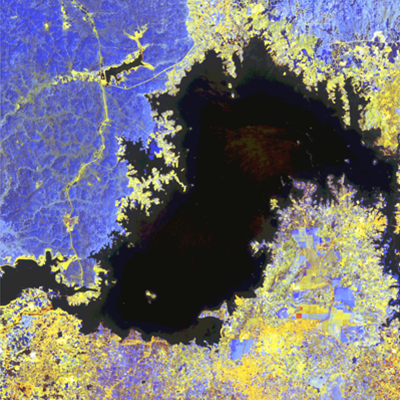
\includegraphics[width=0.7\linewidth]{figures/groud_truth.png}
	\centering
	\caption{Ground Truth}
\end{figure}

\subsubsection{Easiest case: Simple cloud shape}

\begin{figure}[h!]
    \begin{center}
        \begin{tabular}[b]{c}
            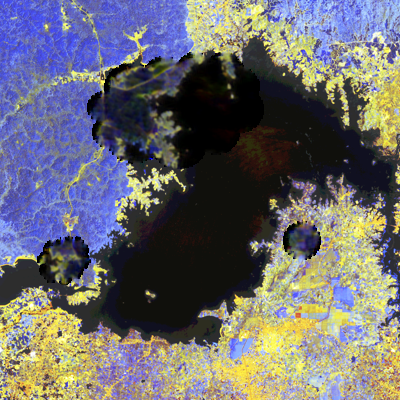
\includegraphics[width=0.3\linewidth]{figures/sts_sample_cloud.png}
          \end{tabular}
          \begin{tabular}[b]{c}
            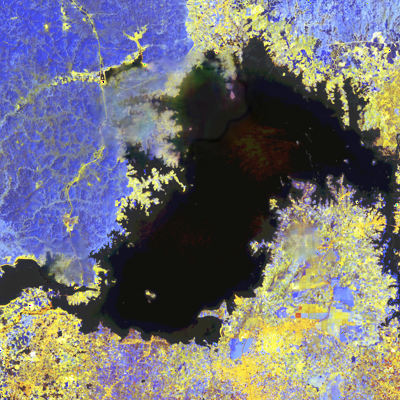
\includegraphics[width=0.3\linewidth]{figures/1_simple.png}
          \end{tabular}
          \begin{tabular}[b]{c}
              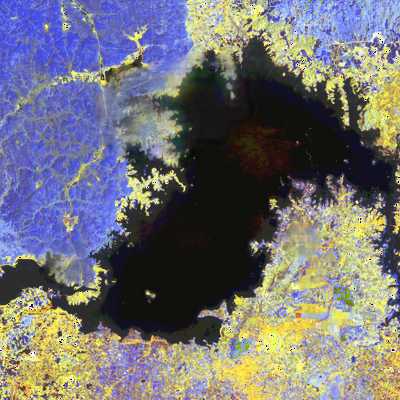
\includegraphics[width=0.3\linewidth]{figures/255_simple.png}
          \end{tabular} 
    \end{center}
	\caption{
		\textbf{(a)} STS-CNN.
		\textbf{(b)} Modified Model, range $0..1$.
		\textbf{(c)} Modified Model, range $0..255$}
	\label{fig:improvedModel_experiment_1}
\end{figure}


\subsubsection{Average case: Multi-simple cloud shape}

\begin{figure}[h!]
    \begin{center}
        \begin{tabular}[b]{c}
            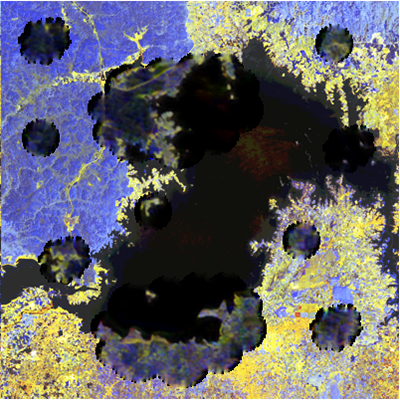
\includegraphics[width=0.3\linewidth]{figures/sts_sample_multicloud.png}
          \end{tabular}
          \begin{tabular}[b]{c}
            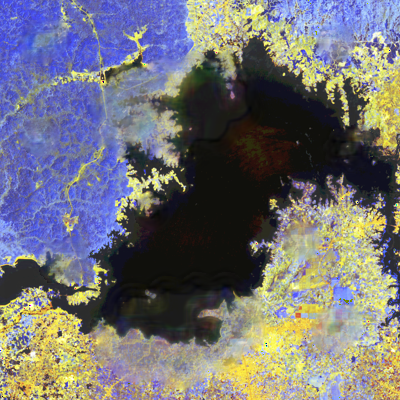
\includegraphics[width=0.3\linewidth]{figures/1_multiFake.png}
          \end{tabular}
          \begin{tabular}[b]{c}
              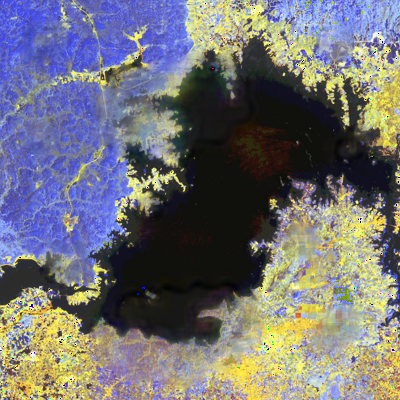
\includegraphics[width=0.3\linewidth]{figures/255_multi_fake.png}
          \end{tabular} 
    \end{center}
    \caption{
		\textbf{(a)} STS-CNN.
		\textbf{(b)} Modified Model, range $0..1$.
		\textbf{(c)} Modified Model, range $0..255$}
	\label{fig:improvedModel_experiment_2}
\end{figure}

\subsubsection{Hardest case: Real cloud}

\begin{figure}[h!]
    \begin{center}
        \begin{tabular}[b]{c}
            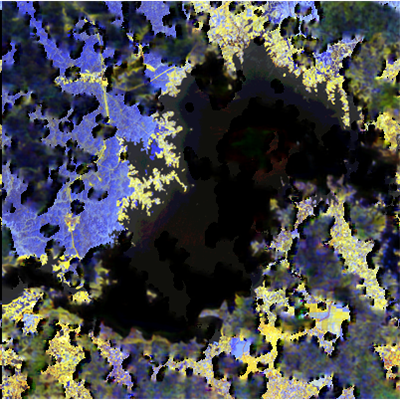
\includegraphics[width=0.3\linewidth]{figures/sts_real_cloud.png}
          \end{tabular}
          \begin{tabular}[b]{c}
            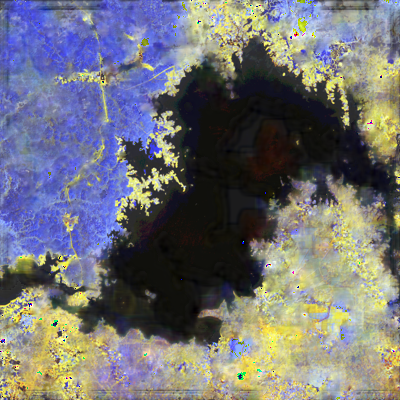
\includegraphics[width=0.3\linewidth]{figures/1_complex.png}
          \end{tabular}
          \begin{tabular}[b]{c}
              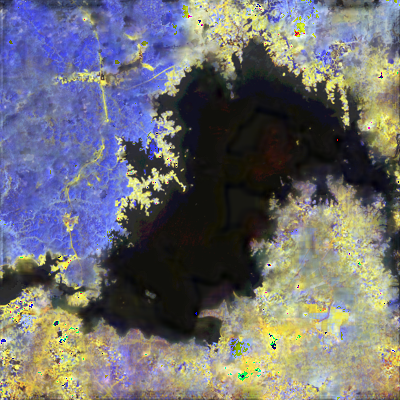
\includegraphics[width=0.3\linewidth]{figures/255_complex.png}
          \end{tabular} 
    \end{center}
    \caption{
		\textbf{(a)} STS-CNN.
		\textbf{(b)} Modified Model, range $0..1$.
		\textbf{(c)} Modified Model, range $0..255$}
	\label{fig:improvedModel_experiment_3}
\end{figure}


\subsection{Trying to recover water body}\label{experiment_timeSeriesModel}
Model has been trained in \textbf{4.1} to take experiments on recovering water body from reconstructed images in cloud days. In order to recover water body, images are collected from Landsat 8 will be crop to be size of $1200 x 1600$ pixels, equals $3 x 4$ tiles, each tiles has size of $400 x 400$ pixels.  

For segmentation, NDWI-index is used to mask out water body. For comparison to ground truth, the most nearest SAR-image collected from Sentinel-1 will be used. 

All Landsat 8 images has been calculated by NDWI formula:

\begin{equation}
NDWI = \frac{Green - Near IR}{Green + Near IR}
\end{equation}

and the display images only contain pixel that having NDWI-index above 0 (which are water or cloud pixel). For Sentinel-1 images, VH-band is used. The pixel belongs to water have value less than -22.

\subparagraph{Explanation for figures} Note that, \textbf{(a)} is covered by cloud, \textbf{(b)} is recovered and \textbf{(c)} is collected from Sentinel-1. 

\begin{figure}[h!]
    \begin{center}
        \begin{tabular}[b]{c}
            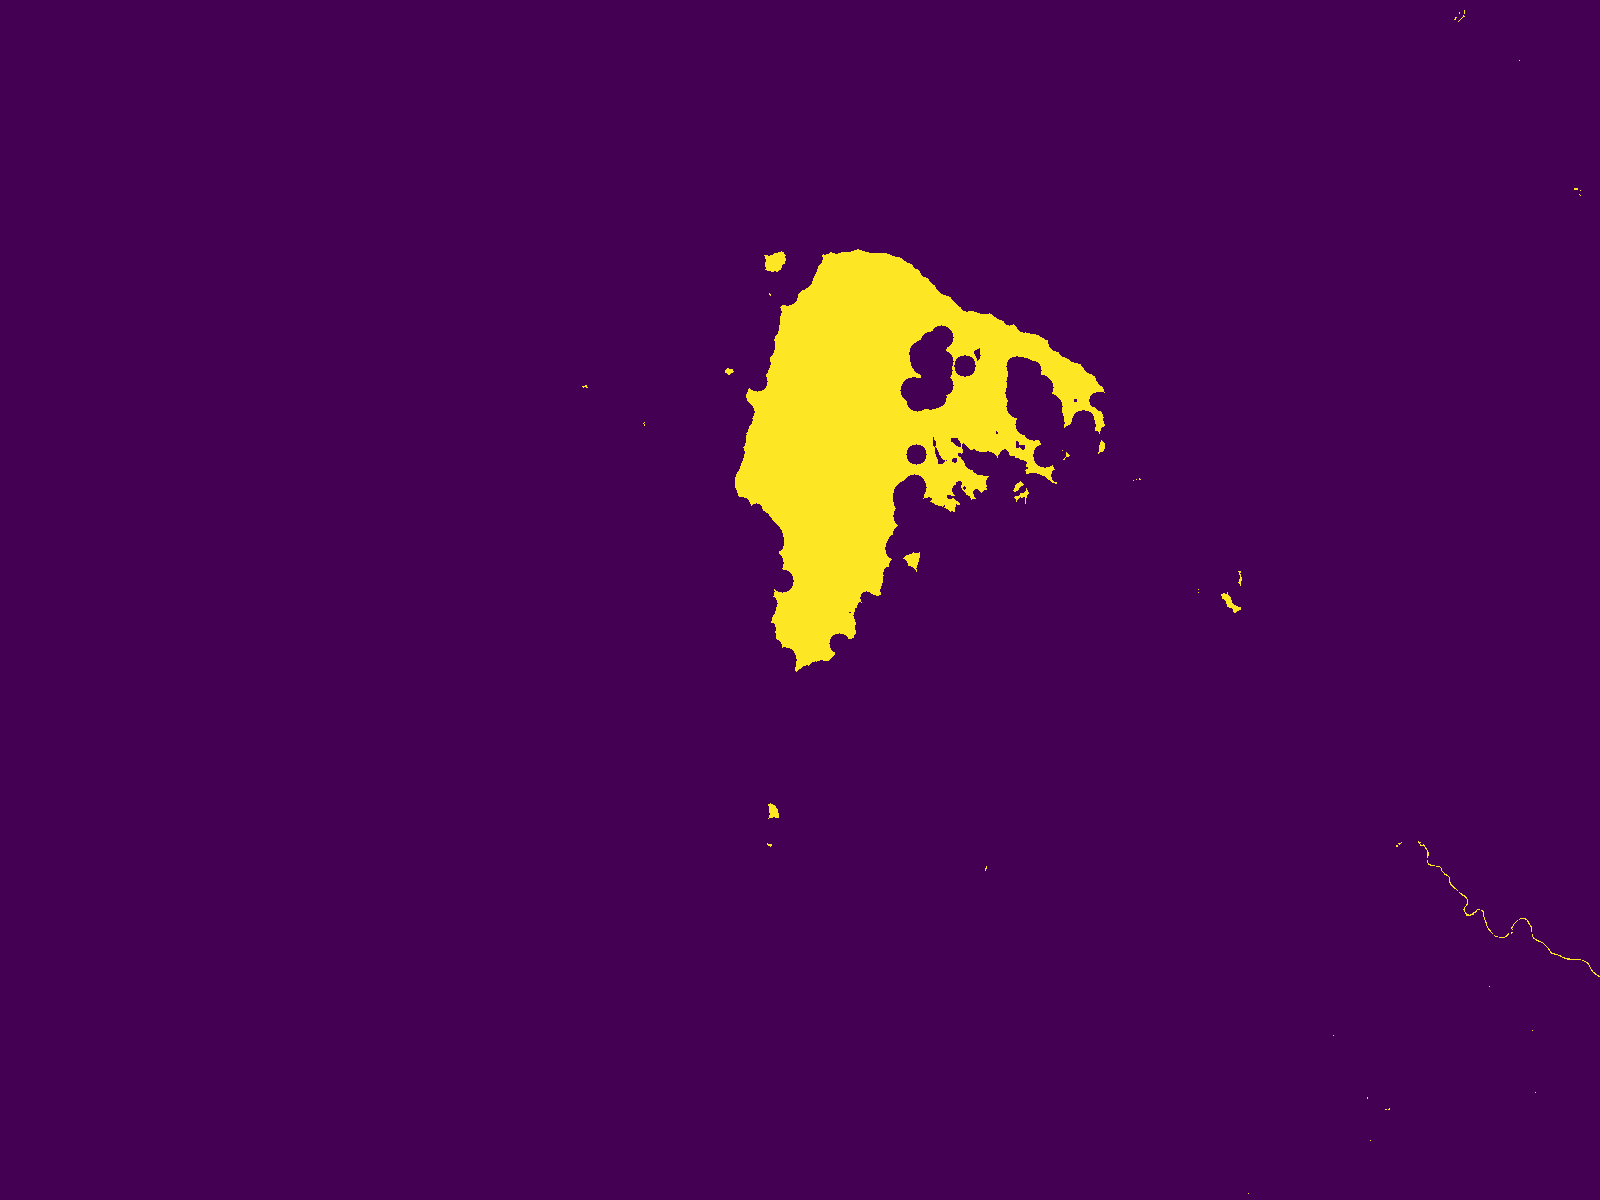
\includegraphics[width=0.3\linewidth]{figures/raw20160104_60_6114.png} \\
            \small (a) 60.6114 $km^2$
          \end{tabular}
          \begin{tabular}[b]{c}
            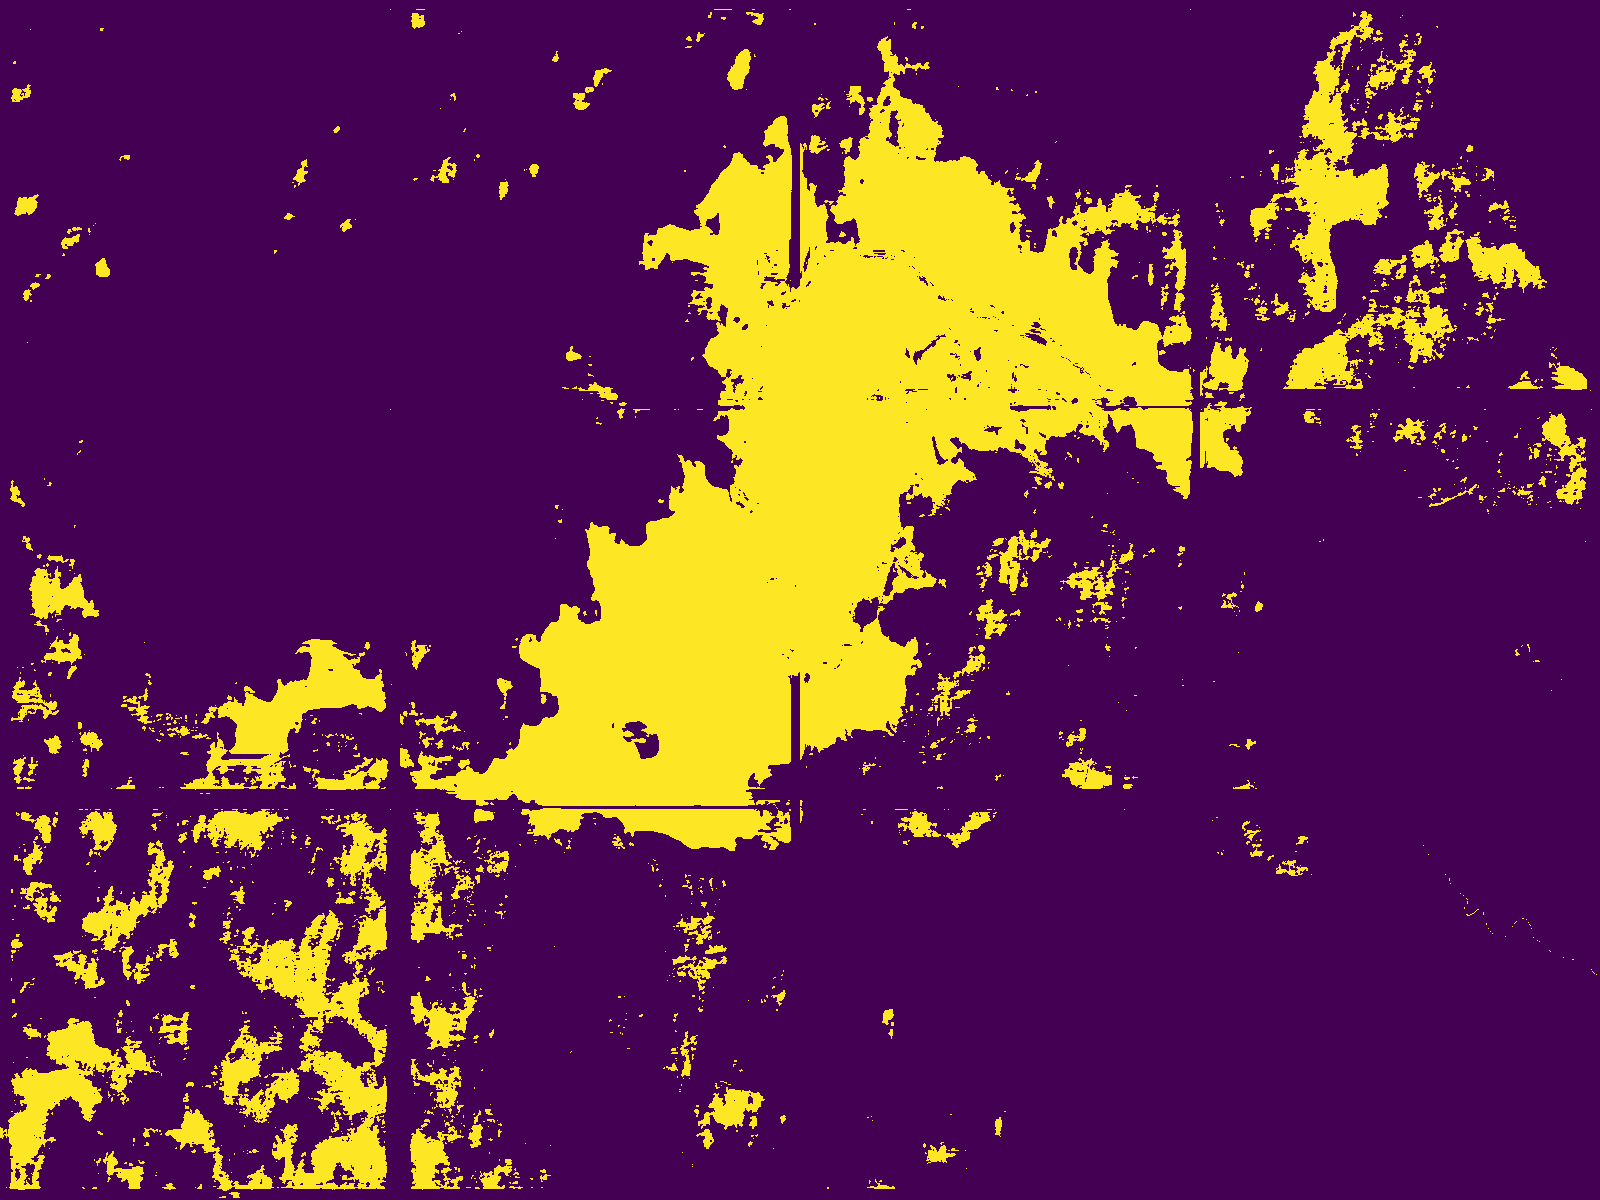
\includegraphics[width=0.3\linewidth]{figures/r20160104_242_0488.png} \\
            \small (b) 242.0488 $km^2$
          \end{tabular}
          \begin{tabular}[b]{c}
              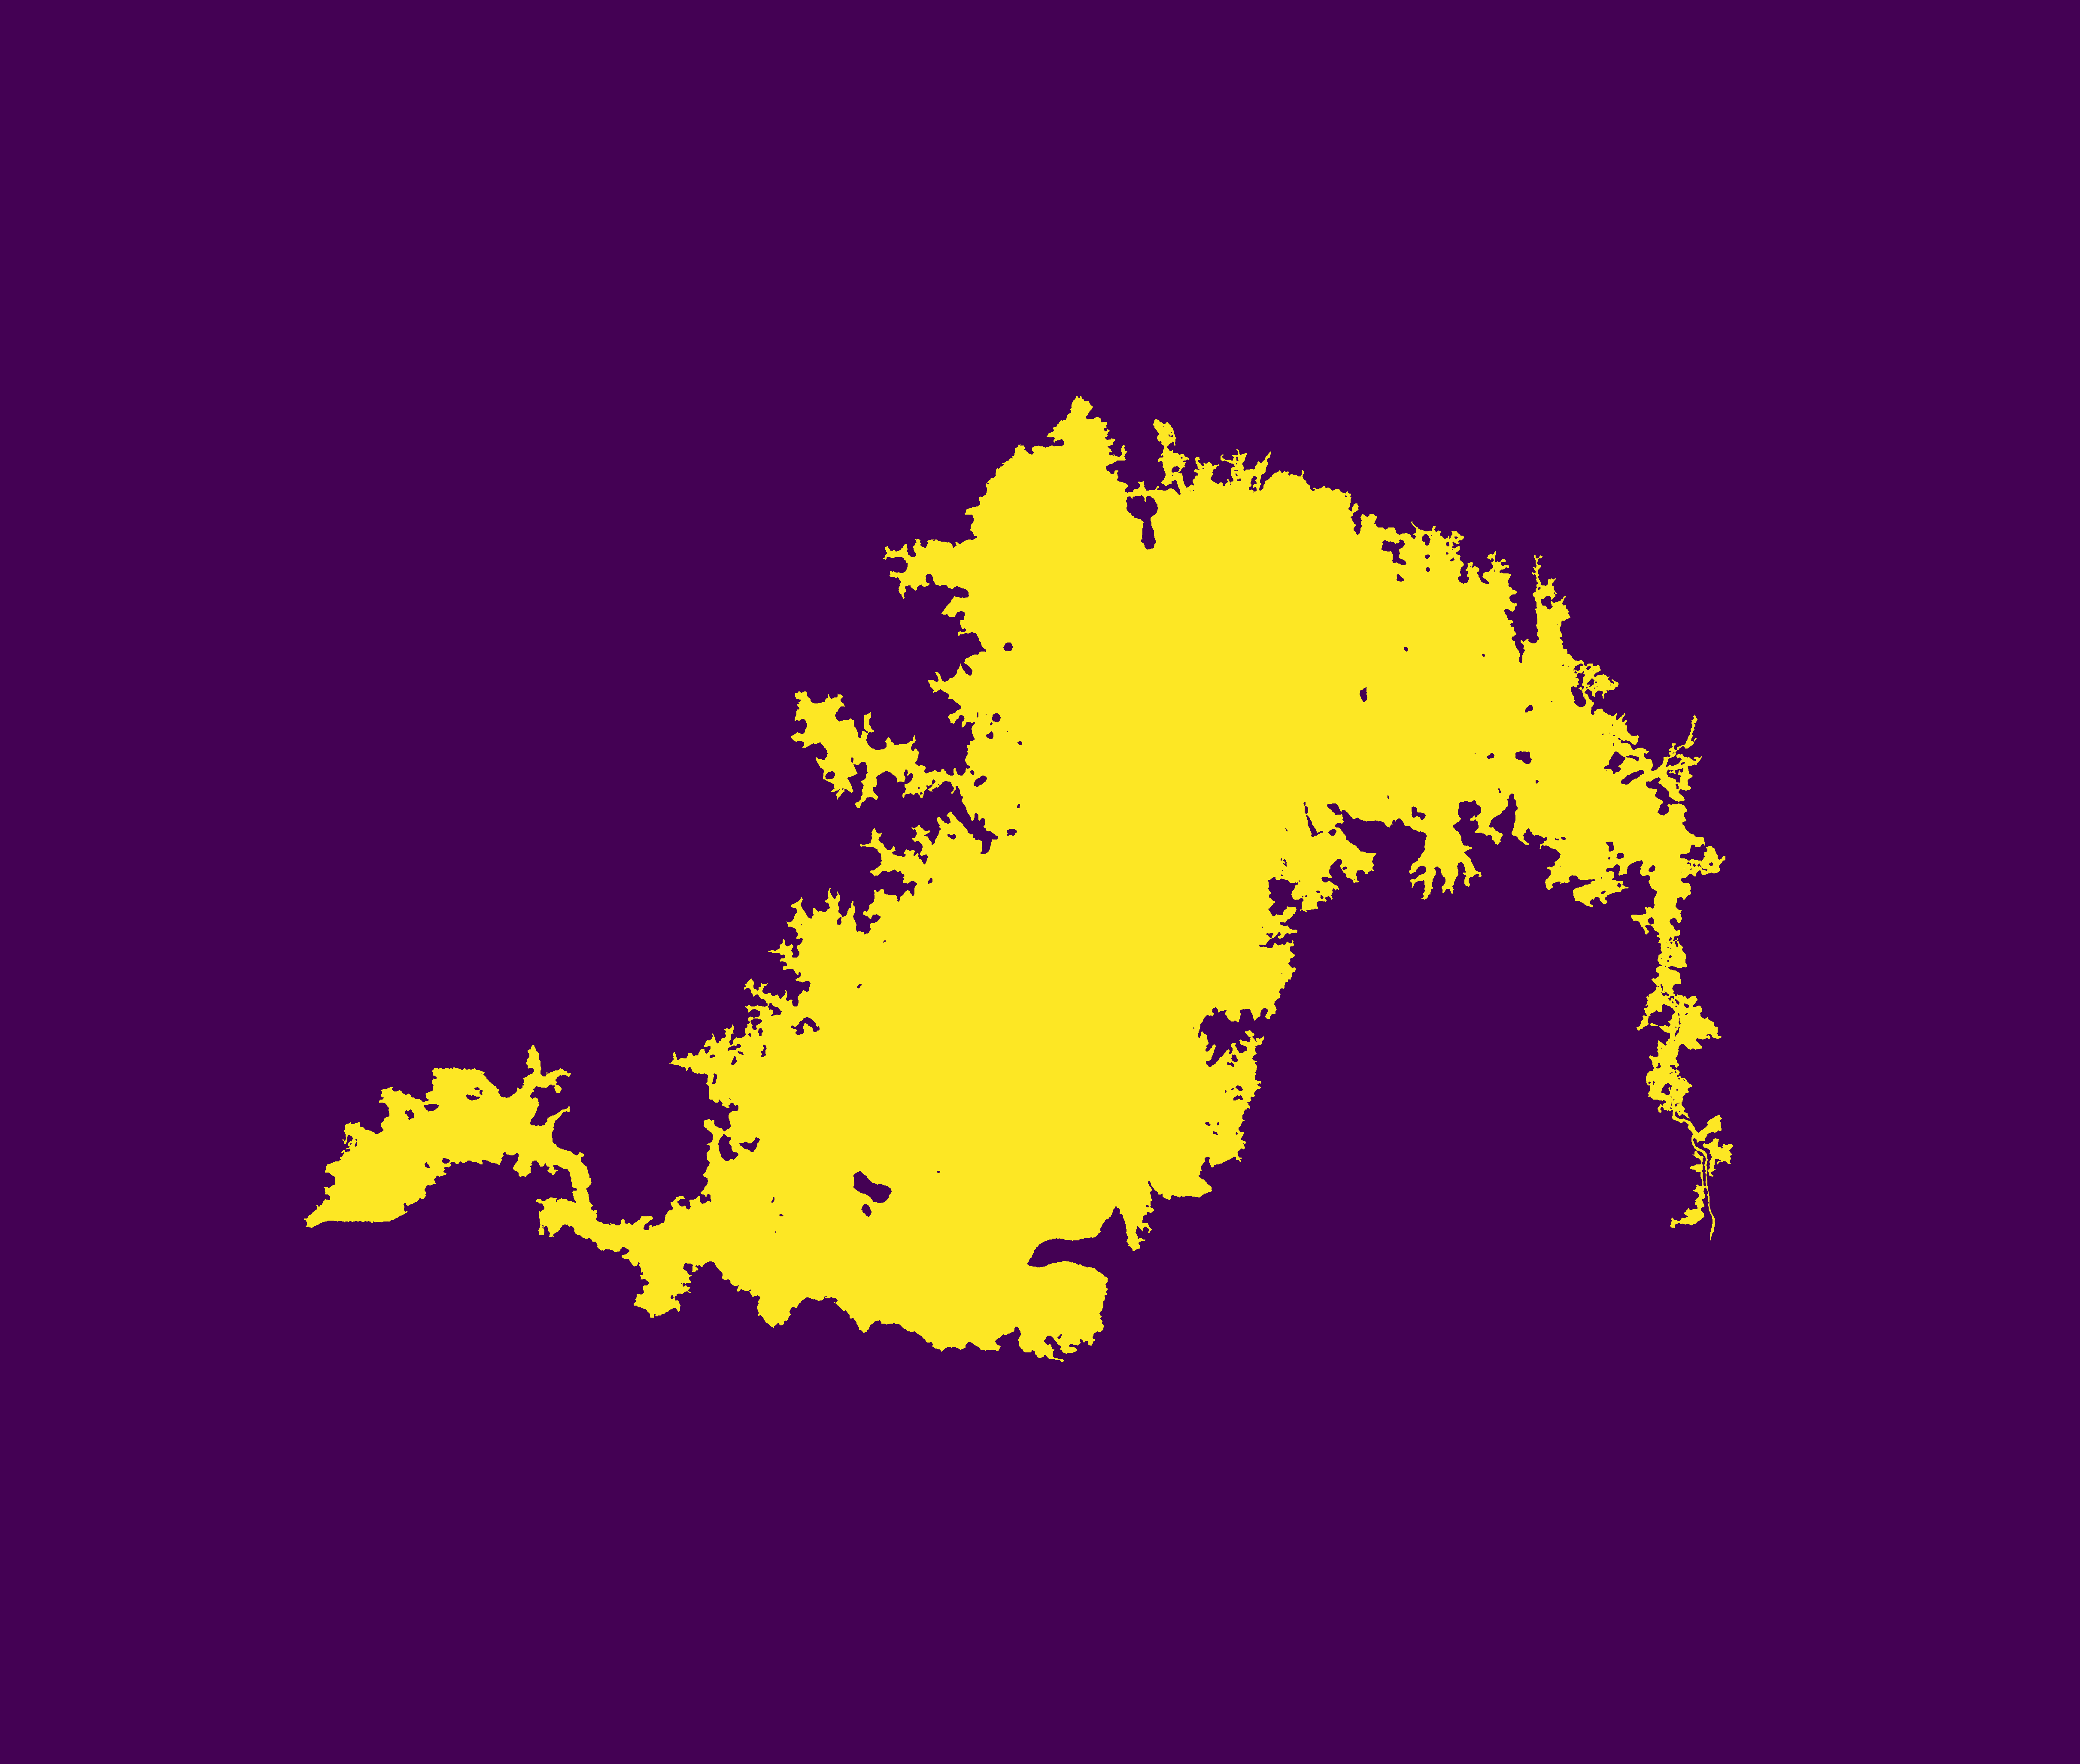
\includegraphics[width=0.3\linewidth]{figures/20160112_269_2041.png} \\
              \small (c) 269.2041 $km^2$
          \end{tabular} 
    \end{center}
    \caption{
		\textbf{(a, b)} Landsat 8, Jan 4th 2016.
		\textbf{(c)} Sentinel-1, Jan 12th 2016.}
\end{figure}

\begin{figure}[h!]
    \begin{center}
        \begin{tabular}[b]{c}
            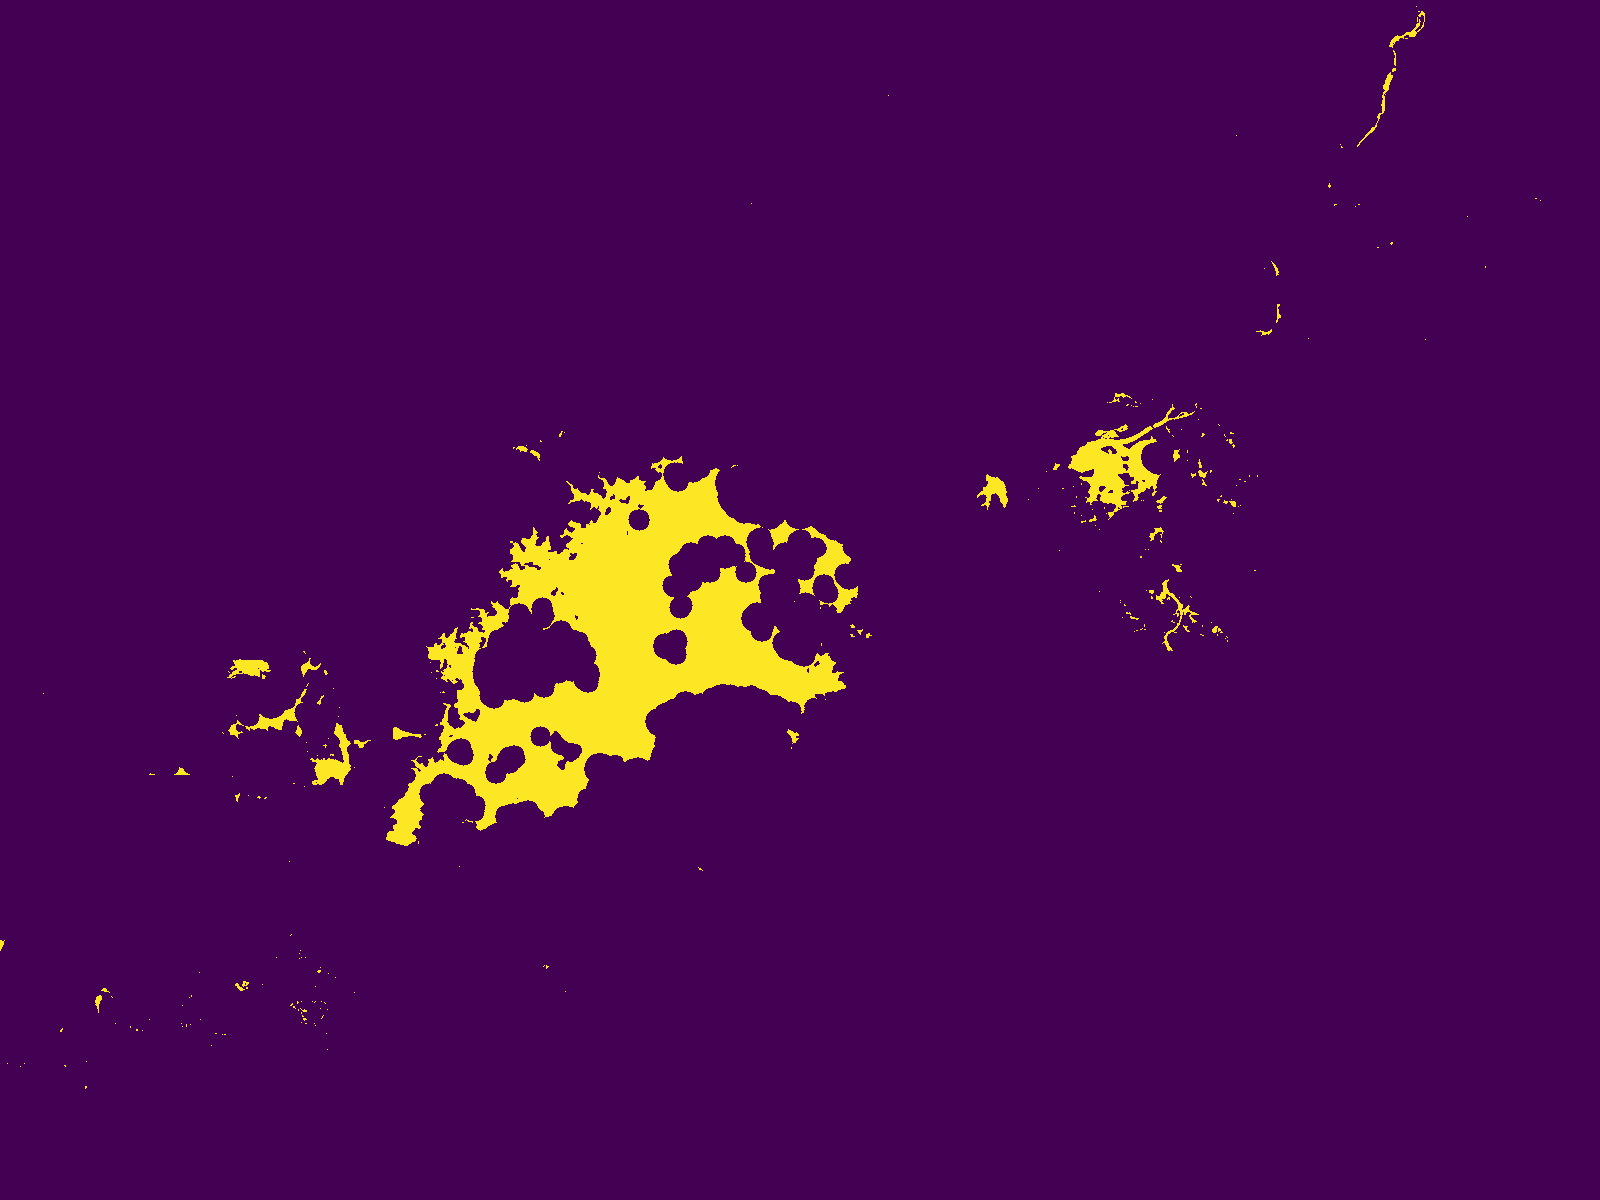
\includegraphics[width=0.3\linewidth]{figures/raw20160815_51_8346.png} \\
            \small (a) 51.8346 $km^2$
          \end{tabular}
          \begin{tabular}[b]{c}
            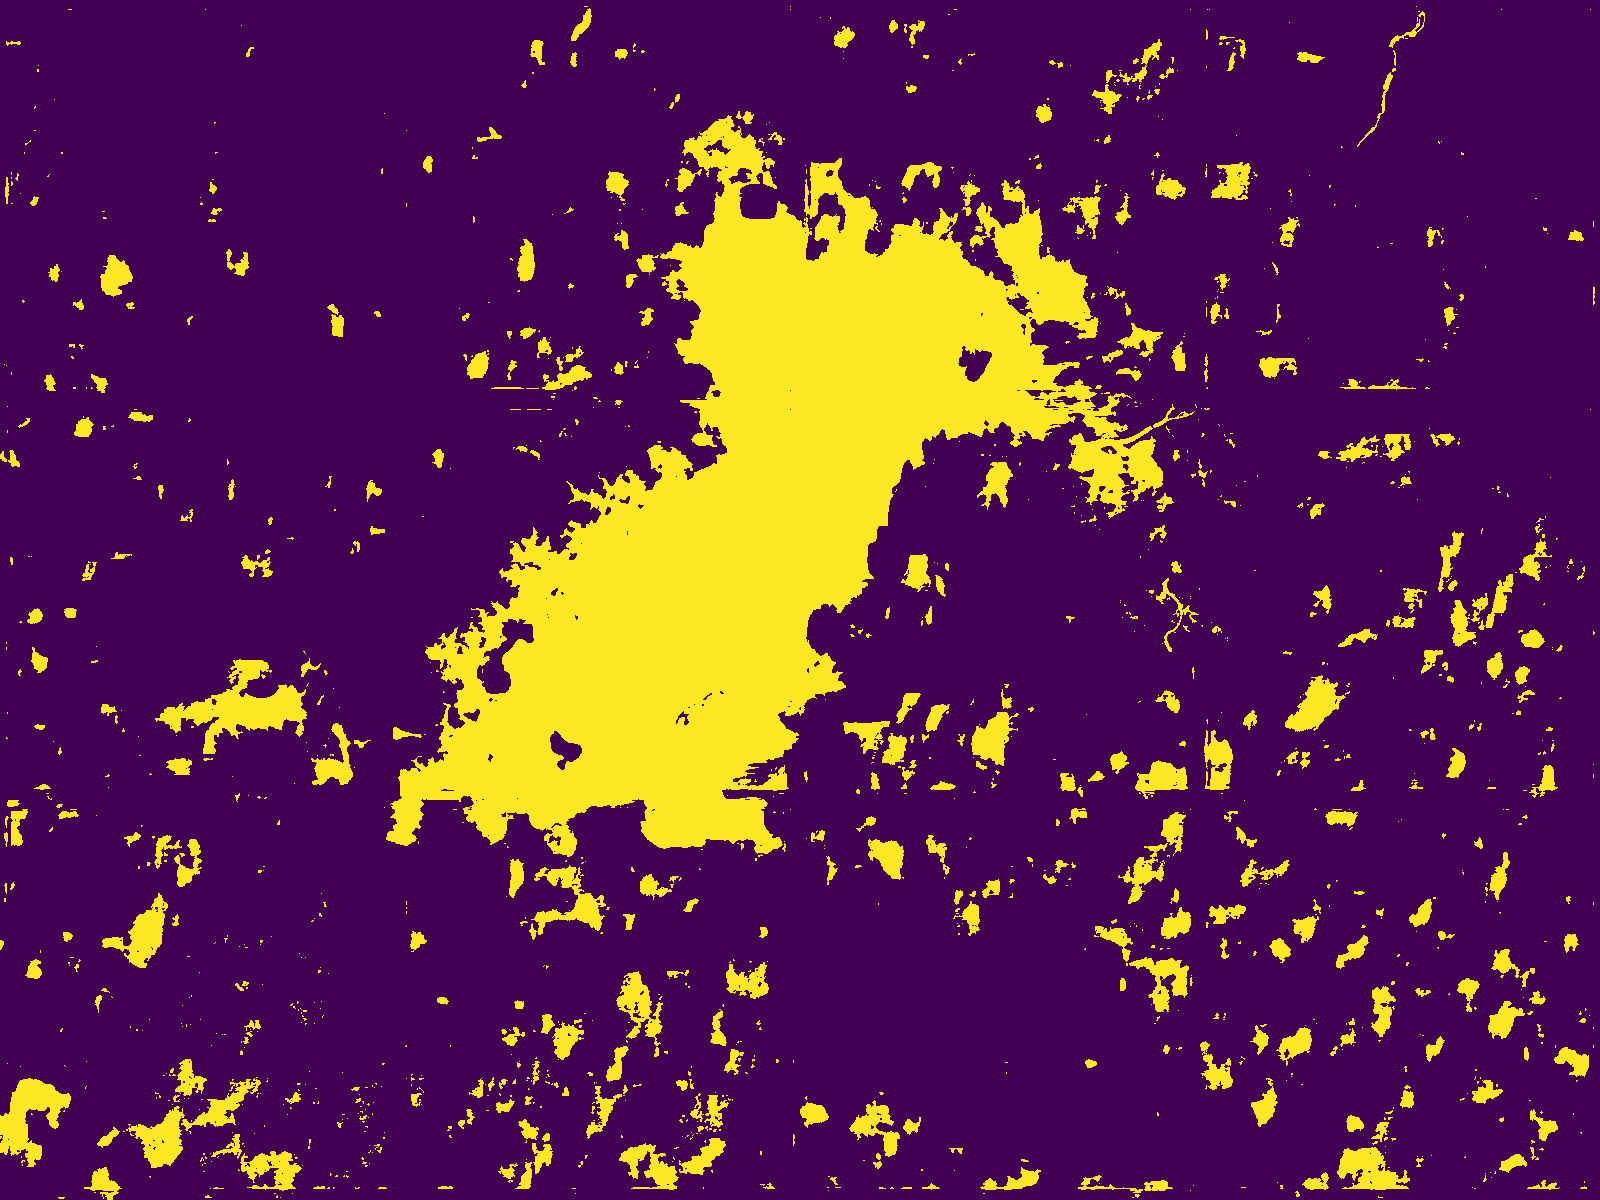
\includegraphics[width=0.3\linewidth]{figures/r20160815_193_9509.png} \\
            \small (b) 193.9509 $km^2$
          \end{tabular}
          \begin{tabular}[b]{c}
              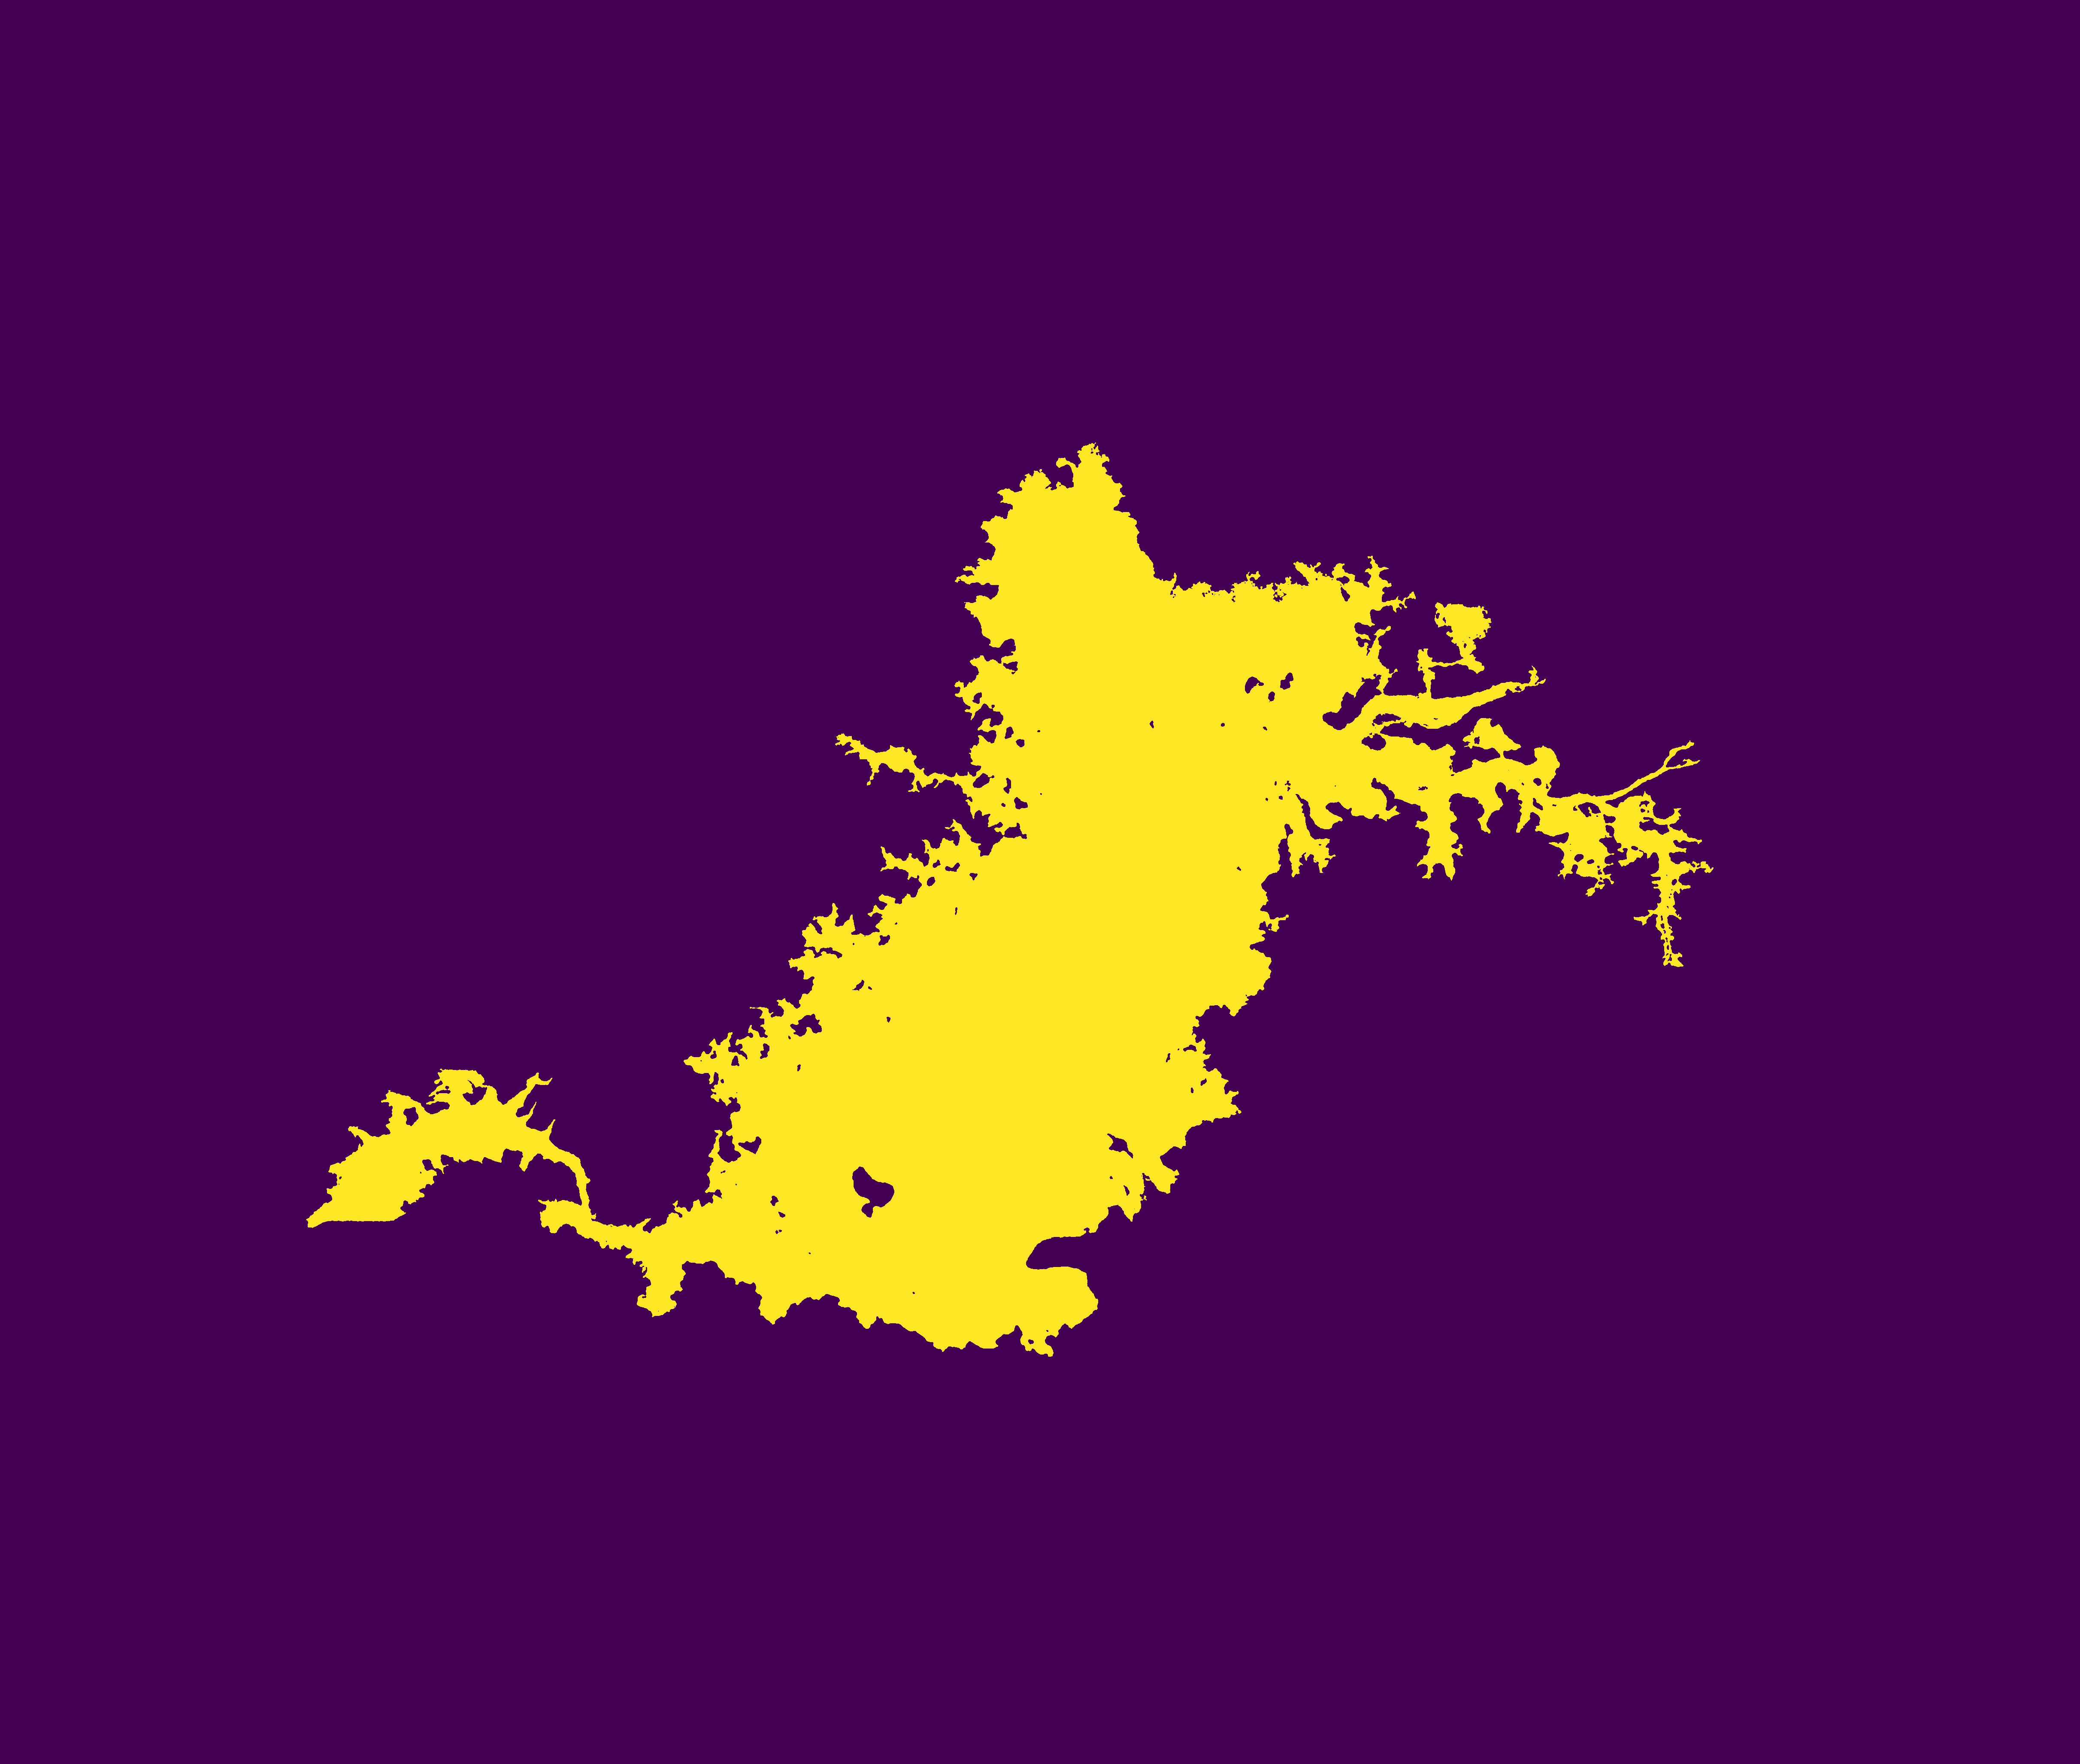
\includegraphics[width=0.3\linewidth]{figures/20160815_201_6019.png} \\
              \small (c) 201.6019 $km^2$
          \end{tabular} 
    \end{center}
    \caption{
		\textbf{(a, b)} Landsat 8, Aug 15th 2016.
		\textbf{(c)} Sentinel-1, Aug 15th 2016.}
\end{figure}

\begin{figure}[h!]
    \begin{center}
        \begin{tabular}[b]{c}
            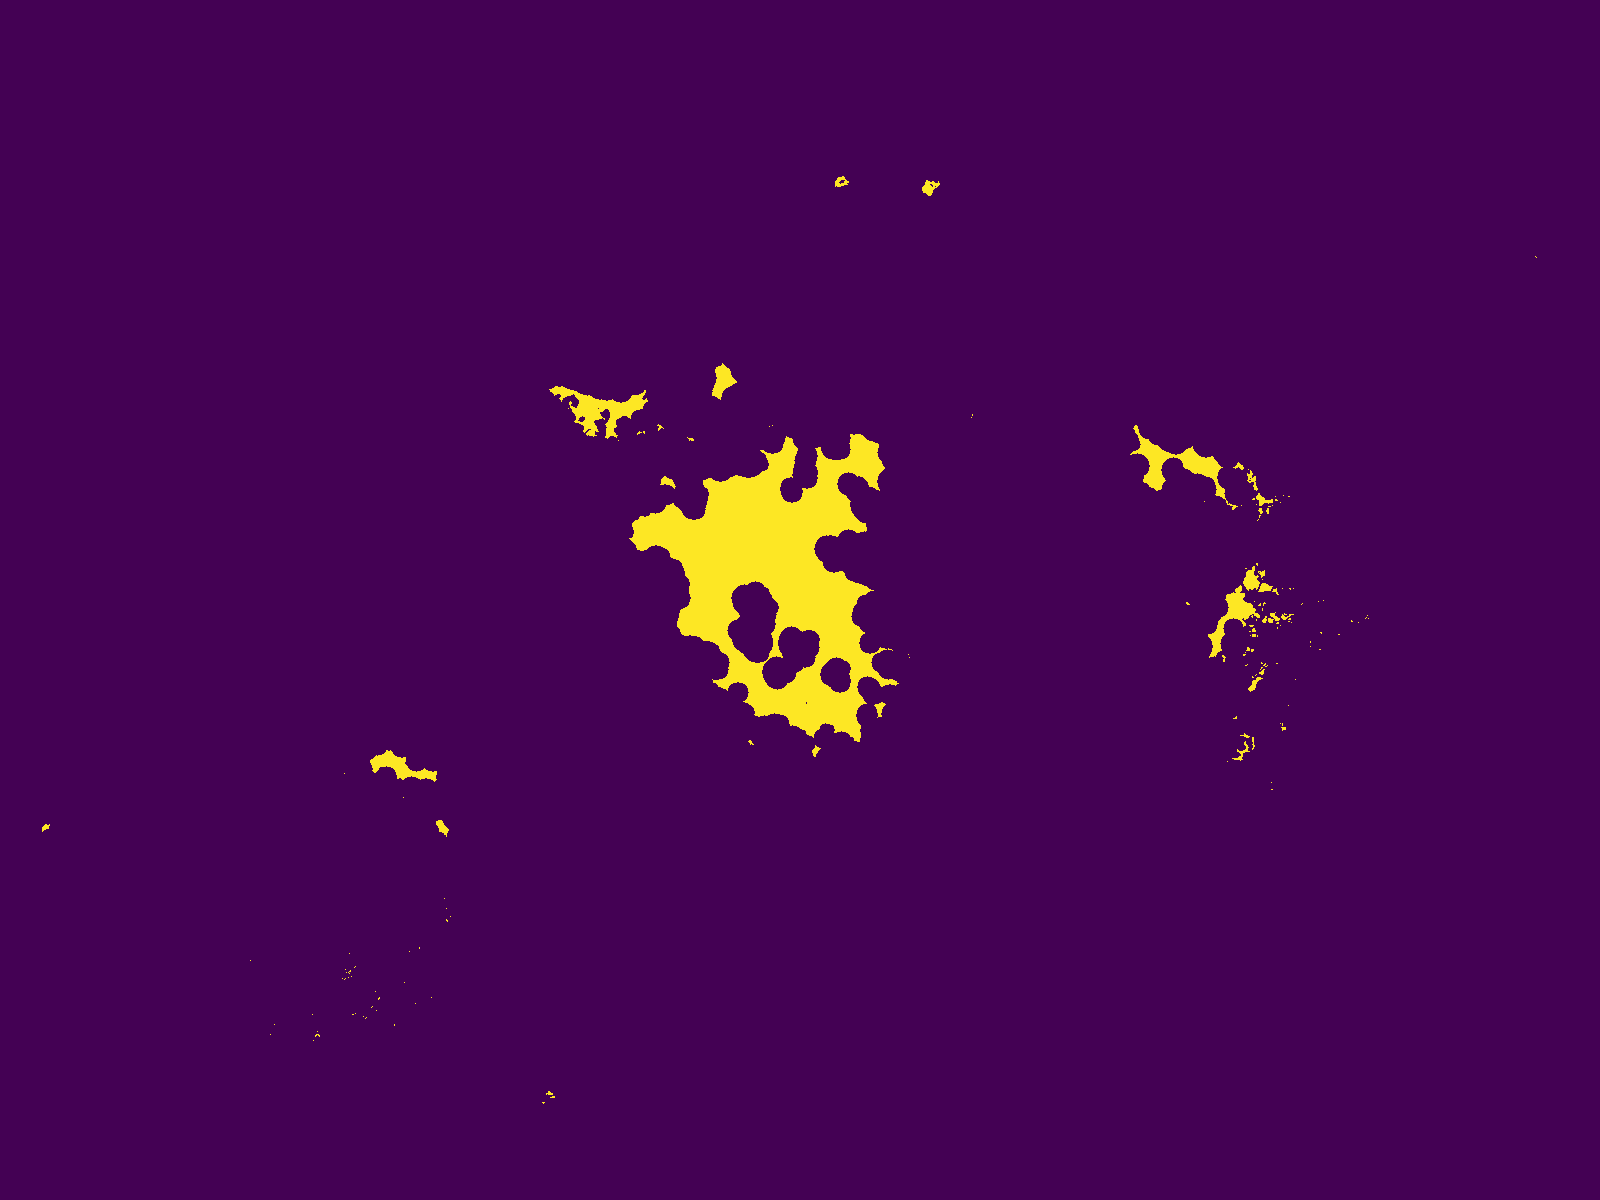
\includegraphics[width=0.3\linewidth]{figures/raw20170802_31_2336.png} \\
            \small (a) 31.2336 $km^2$
          \end{tabular}
          \begin{tabular}[b]{c}
            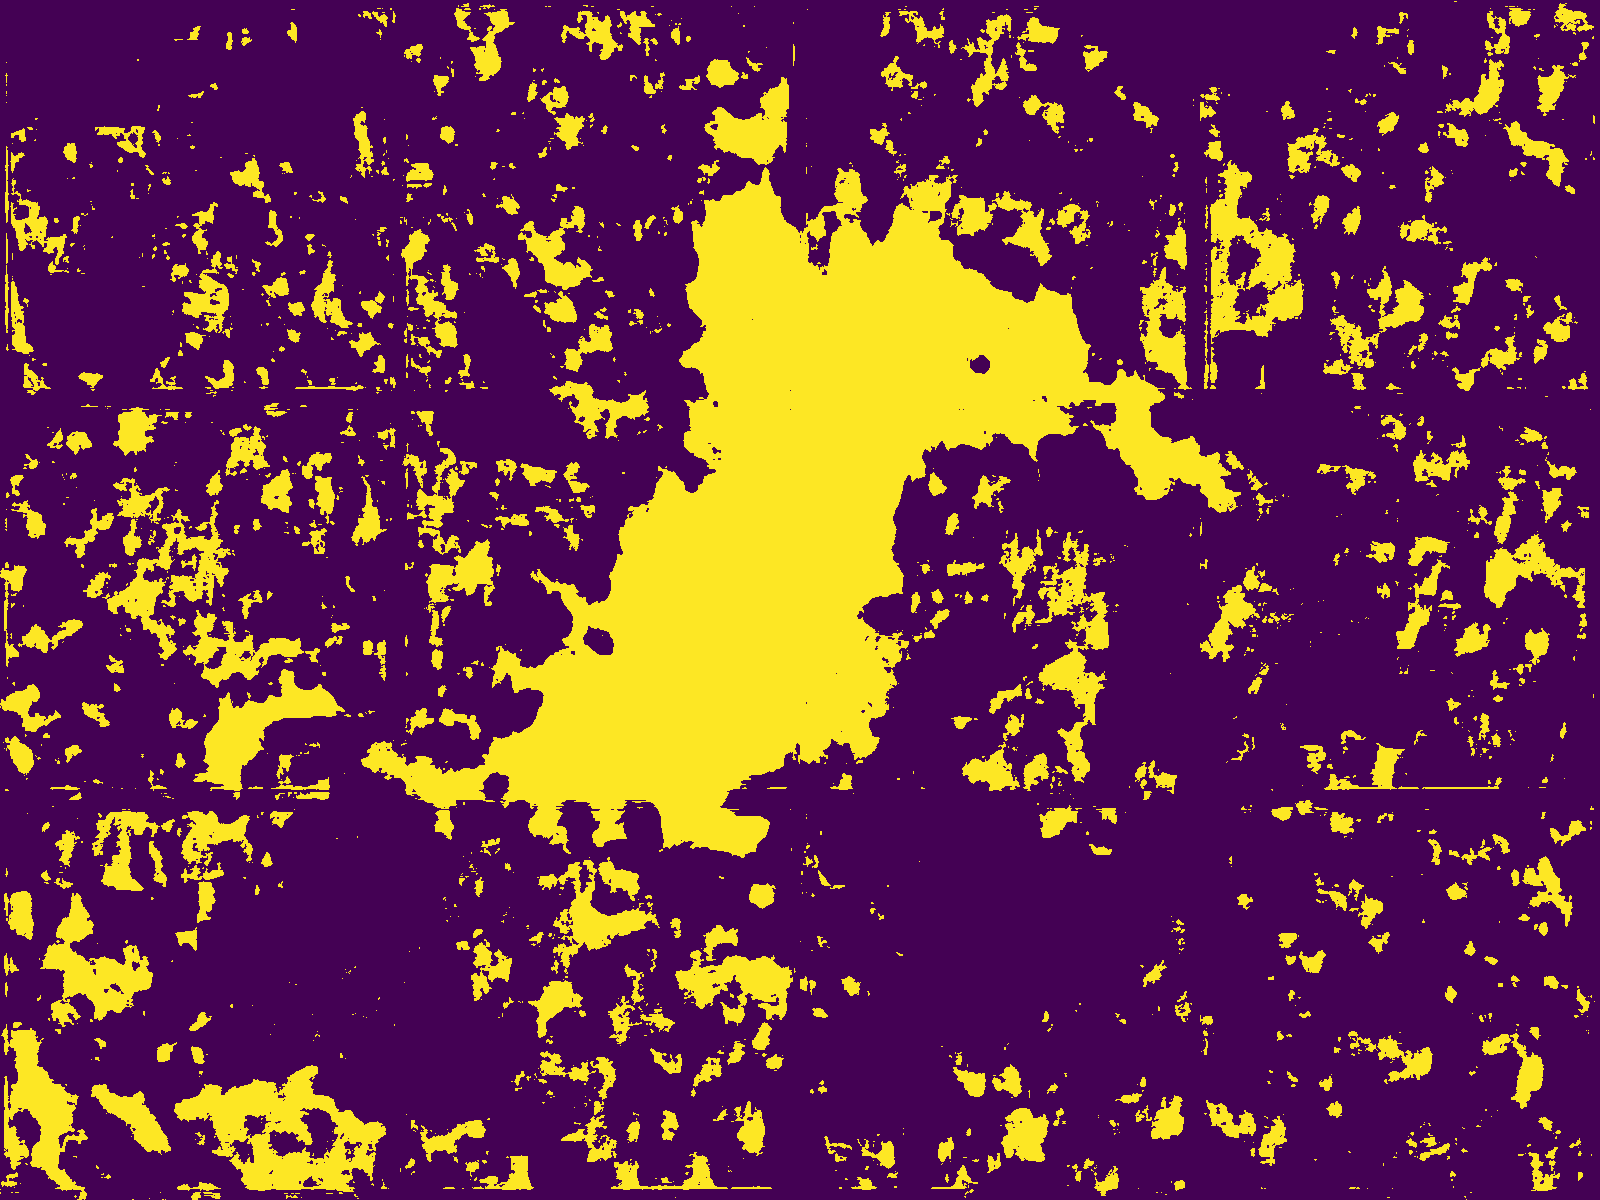
\includegraphics[width=0.3\linewidth]{figures/r20170802_185_7141.png} \\
            \small (b) 185.7141 $km^2$
          \end{tabular}
          \begin{tabular}[b]{c}
              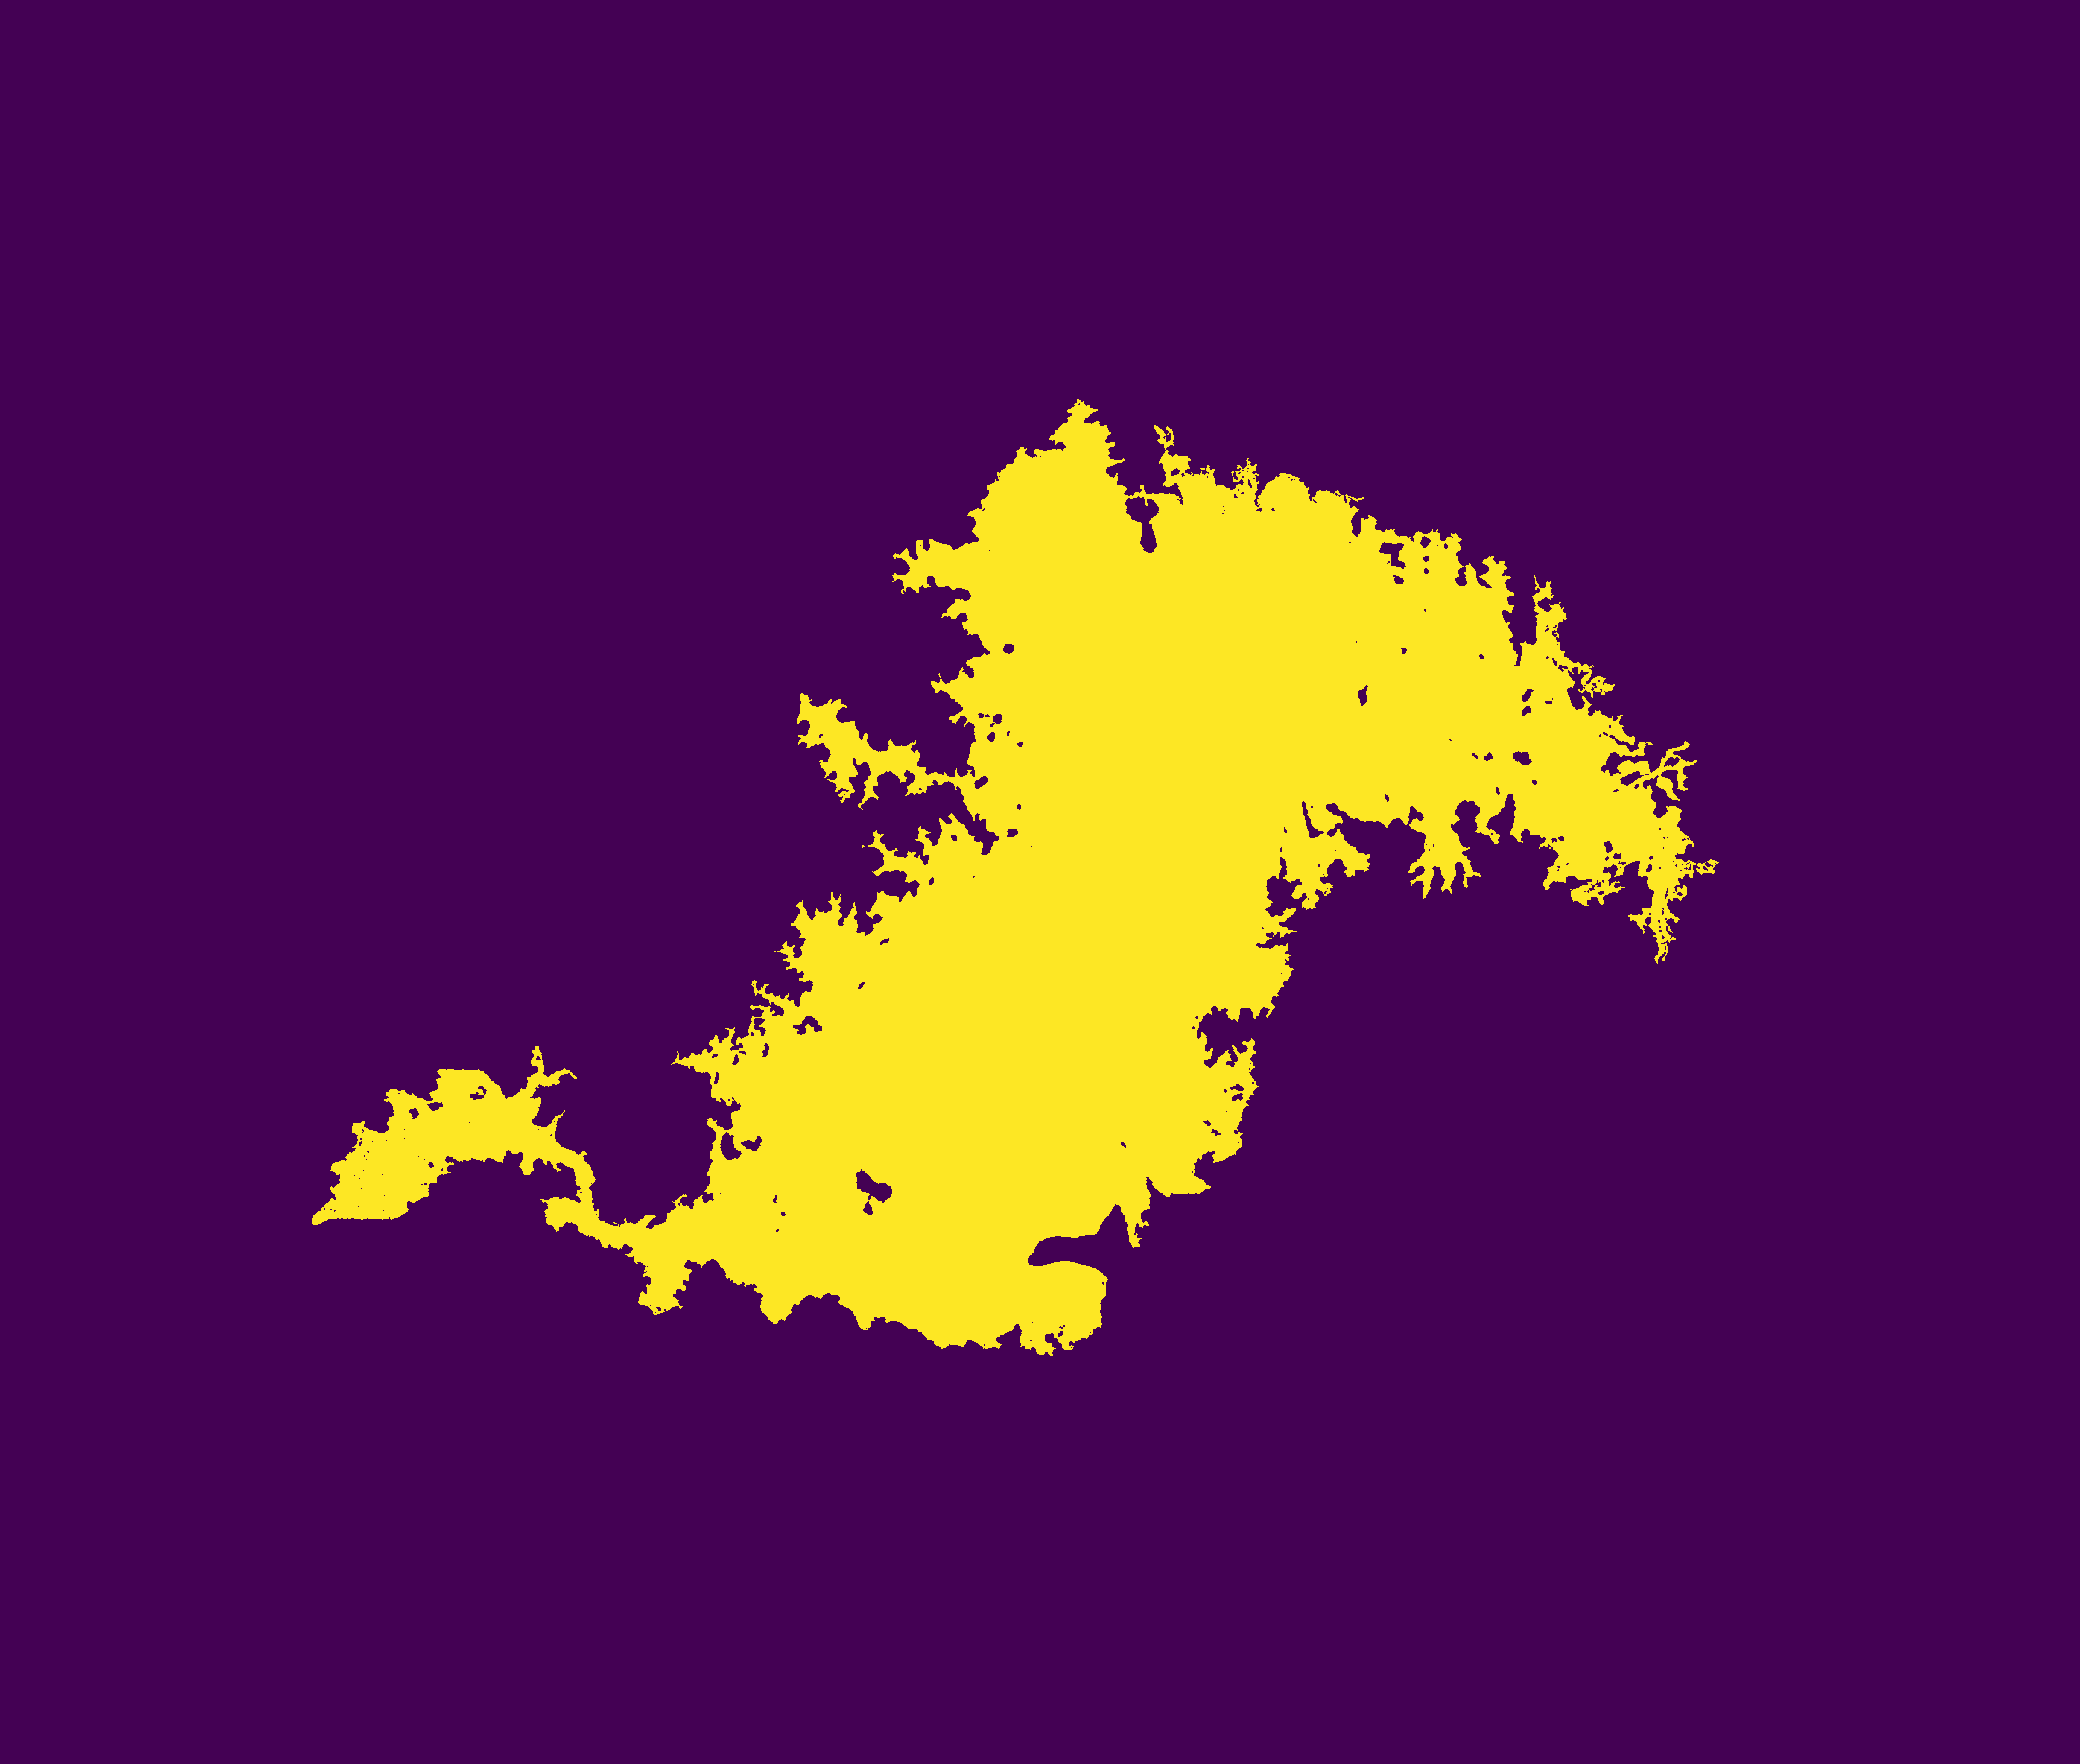
\includegraphics[width=0.3\linewidth]{figures/20170730_258_6828.png} \\
              \small (c) 258.6828 $km^2$
          \end{tabular} 
    \end{center}
    \caption{
		\textbf{(a, b)} Landsat 8, Aug 2nd, 2017.
		\textbf{(c)} Sentinel-1, Jul 30th, 2017.}
\end{figure}


\subsection{Experiments on time-series data}

\subsubsection{Easiest case: Simple cloud shape}

\begin{figure}[h!]
    \begin{center}
        \begin{tabular}[b]{c}
            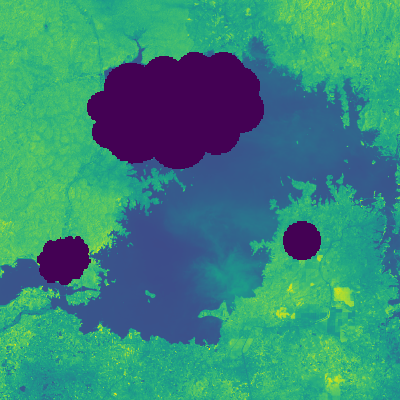
\includegraphics[width=.24\linewidth]{figures/cont5_masked.png}
          \end{tabular}
          \begin{tabular}[b]{c}
            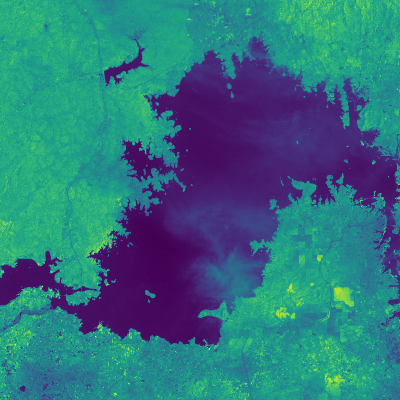
\includegraphics[width=.24\linewidth]{figures/cont5_gt.png}
          \end{tabular}
          \begin{tabular}[b]{c}
              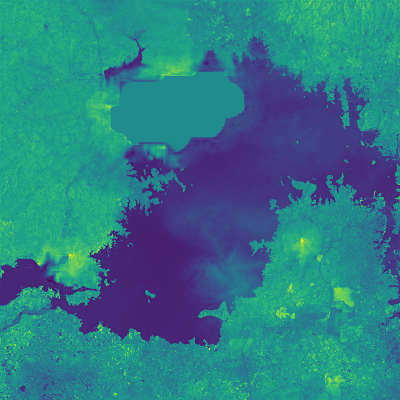
\includegraphics[width=.24\linewidth]{figures/rcnn_simple.png}
		  \end{tabular} 
		  \begin{tabular}[b]{c}
			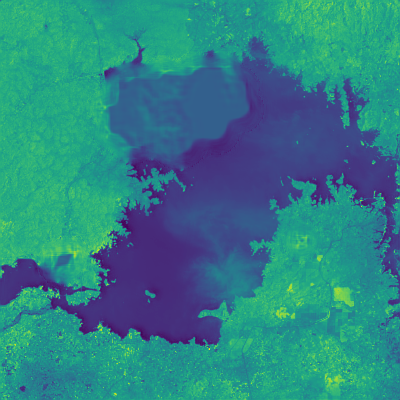
\includegraphics[width=.24\linewidth]{figures/timecnn_simple.png}
		\end{tabular} 
    \end{center}
    \caption{Some clouds with simple shape}
\end{figure}

The result shows that for small regions, both methods could work well, but for a large missing region, it's not easy to get information from time-series images for recovery. Despite higher result in $PSNR$ metric, the recovered region by time-series images look worse than the single image as reference.

\subsubsection{Average case: Multi-simple cloud shape}

\begin{figure}[h!]
    \begin{center}
        \begin{tabular}[b]{c}
            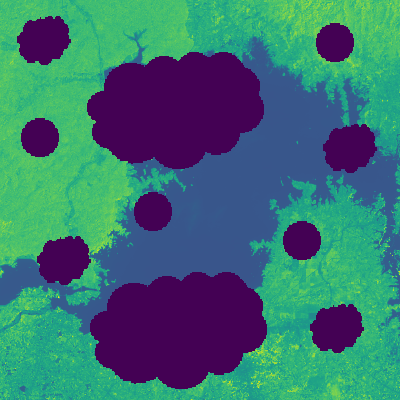
\includegraphics[width=.24\linewidth]{figures/med_1.png}
          \end{tabular}
          \begin{tabular}[b]{c}
            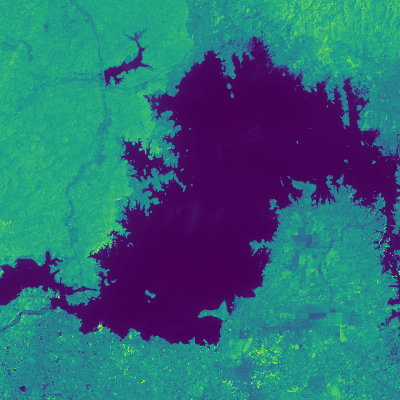
\includegraphics[width=.24\linewidth]{figures/med_2.png}
          \end{tabular}
          \begin{tabular}[b]{c}
              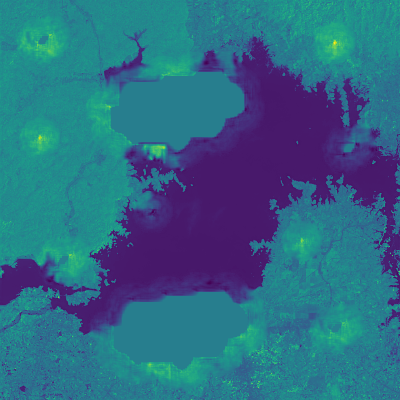
\includegraphics[width=.24\linewidth]{figures/rcnn_med.png}
		  \end{tabular} 
		  \begin{tabular}[b]{c}
			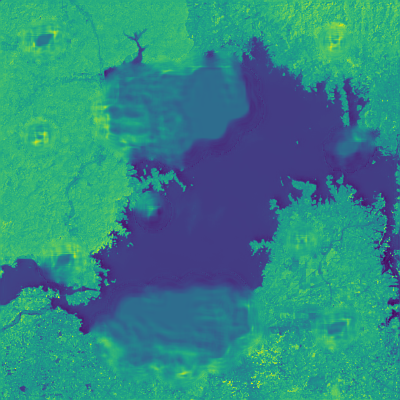
\includegraphics[width=.24\linewidth]{figures/timecnn_med.png}
		\end{tabular} 
    \end{center}
    \caption{The result many clouds, in simple shape}
\end{figure}

\subsubsection{Hardest case: Real cloud}

\begin{figure}[h!]
    \begin{center}
        \begin{tabular}[b]{c}
            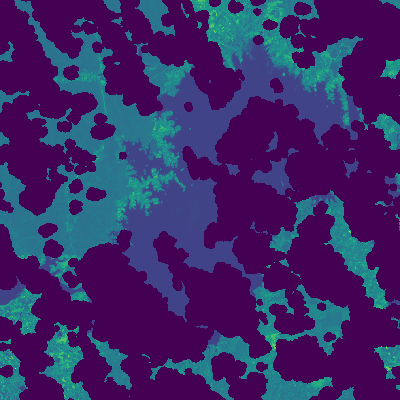
\includegraphics[width=.24\linewidth]{figures/complext_1.png}
          \end{tabular}
          \begin{tabular}[b]{c}
            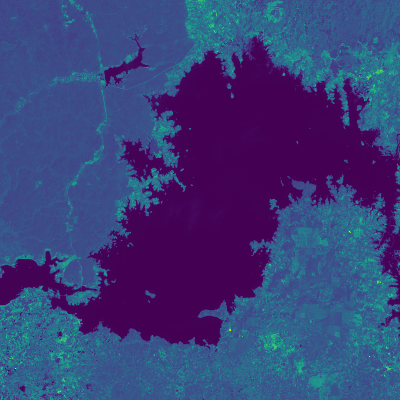
\includegraphics[width=.24\linewidth]{figures/complext_2.png}
          \end{tabular}
          \begin{tabular}[b]{c}
              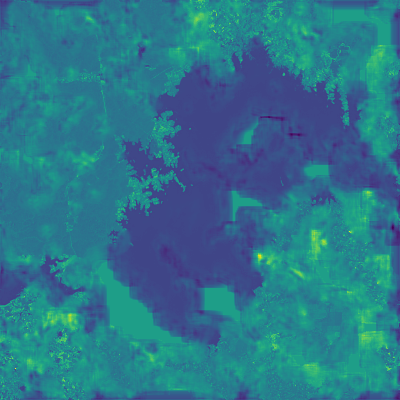
\includegraphics[width=.24\linewidth]{figures/rcnn_complex.png}
		  \end{tabular} 
		  \begin{tabular}[b]{c}
			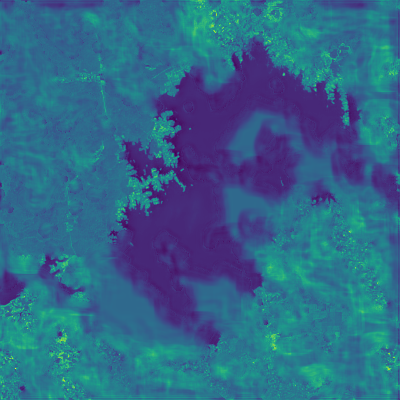
\includegraphics[width=.24\linewidth]{figures/timecnn_complex.png}
		\end{tabular} 
    \end{center}
    \caption{The result on the most complex situation: Real cloud}
\end{figure}


\section{Conclusions}

For optimizing existing method: Scale image to range of $0..1$ slightly get better result than $0..255$. For range of $0..1$, $PSNR$ can be calculated faster as following, because $MAX_I = 1$, so $log_{10}(MAX_I) \textrm{ = } 0$ :

\begin{equation}
\centering
PSNR \textrm{ = } 20 * log_{10}(MAX_I) - 10 * log_{10}(MSE) \textrm{ = } -10 * log_{10}(MSE)
\end{equation}

Seemed to be more complex than original method, the modified model gives better result all over cases. Beside adding more one input to model, we've changed kernel filter of some layers. For some experiments, we found that larger kernel filter size gives better result, but adding more Convolutional layers doesn't. This looks like what mentioned in \textit{Image Super-Resolution Using Deep Convolutional Networks}, Chao et al.

Although the result of reconstruction is quite good when compare to existing method, when taking experiments on real images, it is not as good as expected. It might be quite good if only use it for a look. However, the model could be improved by not resizing the image to $400x400$ size. We could split it to tiles of $400x400$. It is not only keeping the original size, but also keeping details of original images, which is very good for training model.

The result of experiments on time-series images are not as good as expected. Firstly, the input as references for recovery part in network is only one (for a methods in \textbf{Chapter 3.2}, it is two). The second is, the sub-network for prediction is too simple. Itself is a very difficult problem. It is quite similar to a \textit{Moving MNIST problems}, for visualization, see at \href{http://www.cs.toronto.edu/~nitish/unsupervised_video/}{Department of Computer Science, Toronto University}. Some of papers has mentioned about it, for example, \textbf{Convolutional LSTM Network: A Machine Learning Approach for Precipitation Nowcasting}, Xingjian et al. So that, this sub-network have to be considered more complex. 
\chapter{Water level Prediction based on Multi-Spectral Low-resolution Satellite Images }
\label{chap-4-predict-water-body}
\begin{ChapAbstract}
In this chapter, we present our research on predicting the next MODIS image(s) on Tonle Sap lake, especially focusing on water body and shoreline of the lake, and then use this prediction to estimate the future water area of this lake.
\end{ChapAbstract}

\section{Introduction}
Deep learning methods exhibit promising performances for the nearly related problem of our work: video frame prediction. However, the direct adoption of these methods may not yield a sufficient result in satellite image prediction, due to some limitations below:
\begin{enumerate} 
    \item Hydrological status is commonly an annually periodic phenomenon. In contrast, video frame prediction is much focused on objects' movements which usually occur in a short amount of time. Therefore, we need a paradigm which makes used of the periodic property of hydrological data in a more efficient manner.
    \item These methods don't focus on lake's water body which is the main element of this work. A good forecasting in the land region around the lake incorporated with a bad prediction in lake' s water body may cheat us by some good metrics evaluated on the whole image, such as MSE, PSNR, but the final result may not be yielded as expected.
\end{enumerate}
In this chapter, we develop a model which uses the historical MODIS NDVI-band data until timesteps $t$ to predict the MODIS NDVI-band at timesteps $t+1$ with a greater concern for the boundary region of the lake. Our work builds on recent work on using RNNs on 2D sequence data and on using Attention mechanism on time-series data.

Traditional recurrent neural networks only use a fixed-length sequence of \newline
$(x_{t - l + 1}, x_{t - l + 2},\dots,x_{t})$, where $l$ is the sequence length to predict $x_{t + 1}$. It makes RNNs easy to suffer the vanishing gradient problem. Although some advanced RNNs, such as GRU, LSTM, \dots are proved to be capable of reducing this issue, the computational cost is still unnecessarily large. Indeed, the annual periodicity of hydrological status leads to the need of a long input sequence length (it should be at least 46, the number of our MODIS Terra and Aqua data in one year). Loading all of these sequences to GPU wastes a large amount of resources, because each element in an input sequence is used only one time in the forward pass, but GPU must remember them in its memory for the next training epoch.

In order to address these limitations, we propose to use a neural network model which is the fusion of Convolutional LSTM (ConvLSTM) \cite{Shi2015ConvolutionalLN} and Attention mechanism. Instead of directly using a unique long sequence as input, our method divides historical data into multiple small/medium-length input sequences in both long-term and short-term time dependency. The ConvLSTM-based neural networks have the goal of extracting the latent representations of both long and short-term time dependency. Then the attention mechanism is adopted to summary these two temporal latent representations. Finally, a ConvLSTM is used to produce the final prediction.

\section{Data}
\subsection{Study Domain}
This study focuses on the Tonle Sap lake, which is a seasonally inundated freshwater lake in the central low-lying territory of the Cambodia. Our study site was defined by a rectangular boundary of (13.53°N, 103.12°E), (12.42°N, 104.61°E). The Tonle Sap watershed usually experiences two monsoon periods, dry season from December to April and rainy from May to October \cite{article:Hydro-dam-A-nature-based-solution-or-an-ecological-problem}. This great lake functions as a natural reservoir for the Mekong River system during dry season, and regulates flood discharge during wet season. Flood pulse, as a succession of periodic flooding, is the most notable feature of the Tonle Sap Lake. During the dry season, a slow release of the lake water flows into the Mekong through the Tonle Sap River; then the lake is refilled by a reverse water flow from the Mekong during monsoon season, hence forming a globally unique hydrodynamic pattern in the Mekong watershed \cite{article:Socioeconomic-Analysis-Tonle-Sap}.

\subsection{Satellite Observations}
\label{subsection-used-data}
The Moderate Resolution Imaging Spectroradiometer (MODIS), a hyperspectral earth-observing satellite sensor operated by the National Aeronautics and Space Administration (NASA), provides daily satellite coverage, and its VI data products are designed to provide consistent vegetation conditions with spatial resolution ranging from 250 m to 1 km. The 250 m resolution MODIS are Terra (MOD13Q1) and Aqua (MYD13Q1), are valuable source of data in hydrological research. Both data are 16-day composites and are released alternatively (MODIS Terra 's first product in a year is released on 1 Jan, whereas MODIS Aqua 's first product is release on 9 Jan). The combination of these two data provides us a 8-day time-series data, increasing the number of images per year to 46. In this work, we download both MODIS MOD13Q1 and MYD13Q1 data here\footnote{\url{https://modis.ornl.gov}}. Data are collected from 26/6/2002 (near the first released day of MYD13Q1 data) to 31/12/2017 in the Tonle Sap lake region. Finally, we have 714 images of size $513 \times 513$. We use first 576 images for training, 46 next images for validation and last 92 images for testing all baselines and proposed models.
 
\section{Related Work}
Our work builds on recent work in satellite image prediction, video frame prediction, and soft temporal attention that allows modelling the temporal periodicity of weather data.

\textbf{Recurrent Neural Networks in Satellite Image Prediction:} Several pioneering approaches have explored the task of predicting the next satellite image(s) by neural networks. Shi et al. \cite{Shi2015ConvolutionalLN} used a combination of Recurrent Neural Networks and Convolutional Neural Networks to forecast short-term precipitation from temporal radar images. Racah et al. \cite{DBLP:journals/corr/RacahBMPP16} suggested an 3D convolutional auto-encoder (AE) model for extreme weather events detection using 27-years CAM-5 simulation model results.

\textbf{Attention Mechanism in time-series Prediction:} To further imitate the human learning system, attention mechanisms were developed for several existing neural network architectures to determine the importance of different parts of the input during the learning process \cite{Bahdanau2015NeuralMT} \cite{DBLP:journals/corr/XuBKCCSZB15} \cite{DBLP:journals/corr/MnihHGK14} \cite{DBLP:journals/corr/ChenWCGXN15}. Few attempts have been made to employ attention functionality in LSTM in different time-series forecasting problems such as medial diagnosis \cite{DBLP:journals/corr/ChoiBSSS16} and weather forecast \cite{Riemer:2016:CFM:3045390.3045707}. Yao et al. \cite{DBLP:journals/corr/abs-1803-01254} consider the dynamic similarity between locations and propose an attention mechanism (STDN) for LSTM-connected CNNs. Although adding attention mechanism into recurrent architectures improves the performance and comprehensibility, it incurs high computational cost for the whole model (due to the usage of some dense matrices).

This work is inspired by combining ConvLSTM \cite{Shi2015ConvolutionalLN} of Shi et al. and STDN \cite{DBLP:journals/corr/abs-1803-01254} of Yao et al. in order to propose a model that efficiently captures both long-term and short-term temporal dependency and periodicity of remote sensing image data.

\section{Methodology}
\subsection{Model}
Our model mainly consists of 3 parts: the Short-Term Temporal Dependency, the Periodically Shifted Attention Mechanism and the Jointly Training.

Here we define some parameters for our model:
\begin{itemize}
    \item $S$: The length of a period of data (in this work we use $S = 46$, because there are 46 MODIS images in a year, and a year is considered as a period),
    \item $SL$: Input sequence length of short-term part,
    \item $P$: The number of periods (years) used for attention mechanism,
    \item $Q$: The number of relevant timesteps in a period (a year) taken into account the attention mechanism. $Q$ is prefered to be odd,
    \item $FL$: The number of last recent images of timesteps $t$ used as short term-length features for input data of timesteps $t$,
    \item $FH$: The number of previous periods of the period of the timesteps $t$. In these periods, the image, whose internal-period index is similar to the internal-period index of image at timesteps $t$ (or $t \% S$), is taken account to historical features for input data of timesteps $t$. All of these images have the same internal-period index: ($t-S, t-2 \times S,\dots, t-FH \times S$).
\end{itemize}
Let $W, H$ be the shape of an image, $X$ be the set of images from past to present.

\subsubsection{Model input preparation}
\label{model-input-prep}
The model has four inputs, each input is a tensor. Two of them are used for short-term part and the remains are used for long-term part. These inputs can be described in detail as: At timesteps $t$, the label (predicted target) is the image at timesteps $t + 1$, whereas the inputs consist of (for simplicity, batch size is set to 1):
\begin{itemize}
    \item \textbf{short-term CNN feature} $X1$: a tensor with shape $(SL, W, H)$. Each $X1[i,:,:]$ is $X[t - SL + 1 + i]$ for $i$ in $[0, SL - 1]$,
    \item \textbf{short-term LSTM feature} $X2$: a tensor with shape $(SL, W, H, FH+FL)$. For each $i$ in $[0, SL - 1]$, for each $j$ in $[0, FH - 1]$, $X2[i,:,:,j] = X[t - SL + 1 + i - (FH - j)*S]$; for each $j$ in $[0, FL - 1]$, $X_2[i,:,:,FH + j] = X[t - SL + i - FL + j + 2]$,
    \item \textbf{long-term CNN feature} $X3$: a tensor with shape $(P, Q, H, W)$. For each $i$ in $[0, P - 1]$, for each $j$ in $[0, Q - 1]$, $X3[i,j,:,:] = X[t - (P - i)*S + j - Q/2]$, 
    \item \textbf{long-term LSTM feature} $X4$: a tensor with shape $P, Q, H, W, FH + FL$. For each $i$ in $[0, P - 1]$, for each $j$ in $[0, Q - 1]$, let $t_{i, j} = t - (P - i)*S + j - Q/2$, and $X4[i,j, :, :, :]$ is gathered in the same manner as the short-term LSTM feature $X2$ at timesteps $t_{i,j}$ ($X2[t_{i,j},:,:,:]$). 
\end{itemize}
Notice that the smallest image input index is $t - (FH + P)*S - Q/2$, so the smallest timesteps $t$ to be able to generate an input is $t_0 = (FH + P)*S + Q/2$.

\textbf{Concrete Example: }
To clarify the definition of those four inputs, we consider the toy example below. Let $S = 46, SL = 7, P = 3, Q = 3, FL = 4, FH = 3$. $t = t_0 = (FH + P)*S + Q/2 = 277$.
Four inputs of timesteps $t$ are (we only mention the timesteps index):
\begin{itemize}
    \item \textbf{short-term CNN feature:} $X1$ = [270, 271, 272, 273, 274, 275, 276] 
    (see table \ref{tab:Example-short-term-CNN-feature})
    \item \textbf{short-term LSTM feature:} 
    (see table \ref{tab:Example-short-term-LSTM}) \newline
    \[ \begin{array}{ccccccc}
        \mbox{$X2 = \big[$} \big[ 133, & 179, & 225, & 267, & 268, & 269, & 270 \big], \\
        \mbox{\hspace{1.3cm}} \big[ 134, & 180, & 226, & 268, & 269, & 270, & 271 \big],  \\
        \mbox{\hspace{1.3cm}} \big[ 135, & 181, & 227, & 269, & 270, & 271, & 272 \big], \\
        \mbox{\hspace{1.3cm}} \big[ 136, & 182, & 228, & 270, & 271, & 272, & 273 \big], \\
        \mbox{\hspace{1.3cm}} \big[ 137, & 183, & 229, & 271, & 272, & 273, & 274 \big], \\
        \mbox{\hspace{1.3cm}} \big[ 138, & 184, & 230, & 272, & 273, & 274, & 275 \big], \\
        \mbox{\hspace{1.3cm}} \big[ 139, & 185, & 231, & 273, & 274, & 275, & 276 \big] \big]\end{array} \]
    \item \textbf{long-term CNN feature:} \\ $X3 = [[138, 139, 140], [184, 185, 186], [230, 231, 232]]$ (see \ref{tab:Example-long-term-cnn-feature})
    \item \textbf{long-term LSTM feature:} 
    (see table \ref{tab:Example-long-term-LSTM-feature}) \newline
    \[ \begin{array}{lllllll}
        \mbox{$X4 = \big[ \big[$} \big[ 0, & 46, & 92, & 134, & 135, & 136, & 137 \big], \\
        \mbox{\hspace{1.5cm}} \big[ 1, & 47, & 93, & 135, & 136, & 137, & 138 \big], \\
        \mbox{\hspace{1.5cm}} \big[ 2, & 48, & 94, & 136, & 137, & 138, & 139 \big] \big], \\ \\
        \mbox{\hspace{1.1cm} \big[} \big[ 46, & 92, & 138, & 180, & 181, & 182, & 183 \big], \\  
        \mbox{\hspace{1.5cm}}\big[ 47, & 93, & 139, & 181, & 182, & 183, & 184 \big], \\
        \mbox{\hspace{1.5cm}} \big[ 48, & 94, & 140, & 182, & 183, & 184, & 185 \big] \big], \\ \\
        \mbox{\hspace{1.1cm} \big[} \big[ 92, & 138, & 184, & 226, & 227, & 228, & 229 \big], \\  
        \mbox{\hspace{1.5cm}} \big[ 93, & 139, & 185, & 227, & 228, & 229, & 230 \big], \\
        \mbox{\hspace{1.5cm}} \big[ 94, & 140, & 186, & 228, & 229, & 230, & 231 \big] \big] \big]  \end{array} \]
\end{itemize}

% Please add the following required packages to your document preamble:
% \usepackage[table,xcdraw]{xcolor}
% If you use beamer only pass "xcolor=table" option, i.e. \documentclass[xcolor=table]{beamer}
\begin{table}[]
    \begin{tabular}{llllllllllll}
    \hline
    \rowcolor[HTML]{FFFFFF} 
    \multicolumn{1}{|l|}{\cellcolor[HTML]{FFFFFF}0}   & \multicolumn{1}{l|}{\cellcolor[HTML]{FFFFFF}1}   & \multicolumn{1}{l|}{\cellcolor[HTML]{FFFFFF}2}   & \multicolumn{1}{l|}{\cellcolor[HTML]{FFFFFF}…} & \multicolumn{1}{l|}{\cellcolor[HTML]{FFFFFF}38}  & \multicolumn{1}{l|}{\cellcolor[HTML]{FFFFFF}39}  & \multicolumn{1}{l|}{\cellcolor[HTML]{FFFFFF}40}  & \multicolumn{1}{l|}{\cellcolor[HTML]{FFFFFF}41}  & \multicolumn{1}{l|}{\cellcolor[HTML]{FFFFFF}42}  & \multicolumn{1}{l|}{\cellcolor[HTML]{FFFFFF}43}  & \multicolumn{1}{l|}{\cellcolor[HTML]{FFFFFF}44}  & \multicolumn{1}{l|}{\cellcolor[HTML]{FFFFFF}45}  \\ \hline
    \rowcolor[HTML]{FFFFFF} 
    \multicolumn{1}{|l|}{\cellcolor[HTML]{FFFFFF}46}  & \multicolumn{1}{l|}{\cellcolor[HTML]{FFFFFF}47}  & \multicolumn{1}{l|}{\cellcolor[HTML]{FFFFFF}48}  & \multicolumn{1}{l|}{\cellcolor[HTML]{FFFFFF}…} & \multicolumn{1}{l|}{\cellcolor[HTML]{FFFFFF}84}  & \multicolumn{1}{l|}{\cellcolor[HTML]{FFFFFF}85}  & \multicolumn{1}{l|}{\cellcolor[HTML]{FFFFFF}86}  & \multicolumn{1}{l|}{\cellcolor[HTML]{FFFFFF}87}  & \multicolumn{1}{l|}{\cellcolor[HTML]{FFFFFF}88}  & \multicolumn{1}{l|}{\cellcolor[HTML]{FFFFFF}89}  & \multicolumn{1}{l|}{\cellcolor[HTML]{FFFFFF}90}  & \multicolumn{1}{l|}{\cellcolor[HTML]{FFFFFF}91}  \\ \hline
    \rowcolor[HTML]{FFFFFF} 
    \multicolumn{1}{|l|}{\cellcolor[HTML]{FFFFFF}92}  & \multicolumn{1}{l|}{\cellcolor[HTML]{FFFFFF}93}  & \multicolumn{1}{l|}{\cellcolor[HTML]{FFFFFF}94}  & \multicolumn{1}{l|}{\cellcolor[HTML]{FFFFFF}}  & \multicolumn{1}{l|}{\cellcolor[HTML]{FFFFFF}130} & \multicolumn{1}{l|}{\cellcolor[HTML]{FFFFFF}131} & \multicolumn{1}{l|}{\cellcolor[HTML]{FFFFFF}132} & \multicolumn{1}{l|}{\cellcolor[HTML]{FFFFFF}133} & \multicolumn{1}{l|}{\cellcolor[HTML]{FFFFFF}134} & \multicolumn{1}{l|}{\cellcolor[HTML]{FFFFFF}135} & \multicolumn{1}{l|}{\cellcolor[HTML]{FFFFFF}136} & \multicolumn{1}{l|}{\cellcolor[HTML]{FFFFFF}137} \\ \hline
    \rowcolor[HTML]{FFFFFF} 
    \multicolumn{1}{|l|}{\cellcolor[HTML]{FFFFFF}138} & \multicolumn{1}{l|}{\cellcolor[HTML]{FFFFFF}139} & \multicolumn{1}{l|}{\cellcolor[HTML]{FFFFFF}140} & \multicolumn{1}{l|}{\cellcolor[HTML]{FFFFFF}…} & \multicolumn{1}{l|}{\cellcolor[HTML]{FFFFFF}176} & \multicolumn{1}{l|}{\cellcolor[HTML]{FFFFFF}177} & \multicolumn{1}{l|}{\cellcolor[HTML]{FFFFFF}178} & \multicolumn{1}{l|}{\cellcolor[HTML]{FFFFFF}179} & \multicolumn{1}{l|}{\cellcolor[HTML]{FFFFFF}180} & \multicolumn{1}{l|}{\cellcolor[HTML]{FFFFFF}181} & \multicolumn{1}{l|}{\cellcolor[HTML]{FFFFFF}182} & \multicolumn{1}{l|}{\cellcolor[HTML]{FFFFFF}183} \\ \hline
    \rowcolor[HTML]{FFFFFF} 
    \multicolumn{1}{|l|}{\cellcolor[HTML]{FFFFFF}184} & \multicolumn{1}{l|}{\cellcolor[HTML]{FFFFFF}185} & \multicolumn{1}{l|}{\cellcolor[HTML]{FFFFFF}186} & \multicolumn{1}{l|}{\cellcolor[HTML]{FFFFFF}…} & \multicolumn{1}{l|}{\cellcolor[HTML]{FFFFFF}222} & \multicolumn{1}{l|}{\cellcolor[HTML]{FFFFFF}223} & \multicolumn{1}{l|}{\cellcolor[HTML]{FFFFFF}224} & \multicolumn{1}{l|}{\cellcolor[HTML]{FFFFFF}225} & \multicolumn{1}{l|}{\cellcolor[HTML]{FFFFFF}226} & \multicolumn{1}{l|}{\cellcolor[HTML]{FFFFFF}227} & \multicolumn{1}{l|}{\cellcolor[HTML]{FFFFFF}228} & \multicolumn{1}{l|}{\cellcolor[HTML]{FFFFFF}229} \\ \hline
    \rowcolor[HTML]{FFFFFF} 
    \multicolumn{1}{|l|}{\cellcolor[HTML]{FFFFFF}230} & \multicolumn{1}{l|}{\cellcolor[HTML]{FFFFFF}231} & \multicolumn{1}{l|}{\cellcolor[HTML]{FFFFFF}232} & \multicolumn{1}{l|}{\cellcolor[HTML]{FFFFFF}}  & \multicolumn{1}{l|}{\cellcolor[HTML]{FFFFFF}268} & \multicolumn{1}{l|}{\cellcolor[HTML]{FFFFFF}269} & \multicolumn{1}{l|}{\cellcolor[HTML]{FFCB2F}270} & \multicolumn{1}{l|}{\cellcolor[HTML]{FFCB2F}271} & \multicolumn{1}{l|}{\cellcolor[HTML]{FFCB2F}272} & \multicolumn{1}{l|}{\cellcolor[HTML]{FFCB2F}273} & \multicolumn{1}{l|}{\cellcolor[HTML]{FFCB2F}274} & \multicolumn{1}{l|}{\cellcolor[HTML]{FFCB2F}275} \\ \hline
    \rowcolor[HTML]{FFFFFF} 
    \multicolumn{1}{|l|}{\cellcolor[HTML]{FFCC67}276} & \multicolumn{1}{l|}{\cellcolor[HTML]{34FF34}277} & \multicolumn{1}{l|}{\cellcolor[HTML]{FFFFFF}278} & \multicolumn{1}{l|}{\cellcolor[HTML]{FFFFFF}…} & \multicolumn{1}{l|}{\cellcolor[HTML]{FFFFFF}314} & \multicolumn{1}{l|}{\cellcolor[HTML]{FFFFFF}315} & \multicolumn{1}{l|}{\cellcolor[HTML]{FFFFFF}316} & \multicolumn{1}{l|}{\cellcolor[HTML]{FFFFFF}317} & \multicolumn{1}{l|}{\cellcolor[HTML]{FFFFFF}318} & \multicolumn{1}{l|}{\cellcolor[HTML]{FFFFFF}319} & \multicolumn{1}{l|}{\cellcolor[HTML]{FFFFFF}320} & \multicolumn{1}{l|}{\cellcolor[HTML]{FFFFFF}321} \\ \hline
                                                      &                                                  &                                                  &                                                &                                                  &                                                  &                                                  &                                                  &                                                  &                                                  &                                                  &                                                  \\
                                                      &                                                  &                                                  &                                                &                                                  & \cellcolor[HTML]{34FF34}                         & \multicolumn{6}{l}{target timesteps}                                                                                                                                                                                                                                                                             \\
                                                      &                                                  &                                                  &                                                &                                                  & \cellcolor[HTML]{FFCC67}                         & \multicolumn{6}{l}{short-term-cnn feature X1}                                                                                                                                                                                                                                                                  
    \end{tabular}
    \caption{Example of short-term CNN feature at timesteps 277}
    \label{tab:Example-short-term-CNN-feature}
    \end{table}

\begin{table}[]
    \begin{tabular}{llllllllllll}
    \hline
    \multicolumn{1}{|l|}{0}                           & \multicolumn{1}{l|}{1}                           & \multicolumn{1}{l|}{2}                           & \multicolumn{1}{l|}{…}                         & \multicolumn{1}{l|}{38}                          & \multicolumn{1}{l|}{39}                          & \multicolumn{1}{l|}{40}                          & \multicolumn{1}{l|}{41}                          & \multicolumn{1}{l|}{42}                          & \multicolumn{1}{l|}{43}                          & \multicolumn{1}{l|}{44}                          & \multicolumn{1}{l|}{45}                          \\ \hline
    \multicolumn{1}{|l|}{46}                          & \multicolumn{1}{l|}{47}                          & \multicolumn{1}{l|}{48}                          & \multicolumn{1}{l|}{…}                         & \multicolumn{1}{l|}{84}                          & \multicolumn{1}{l|}{85}                          & \multicolumn{1}{l|}{86}                          & \multicolumn{1}{l|}{87}                          & \multicolumn{1}{l|}{88}                          & \multicolumn{1}{l|}{89}                          & \multicolumn{1}{l|}{90}                          & \multicolumn{1}{l|}{91}                          \\ \hline
    \multicolumn{1}{|l|}{92}                          & \multicolumn{1}{l|}{93}                          & \multicolumn{1}{l|}{94}                          & \multicolumn{1}{l|}{}                          & \multicolumn{1}{l|}{130}                         & \multicolumn{1}{l|}{131}                         & \multicolumn{1}{l|}{132}                         & \multicolumn{1}{l|}{133}                         & \multicolumn{1}{l|}{\cellcolor[HTML]{FFFFC7}134} & \multicolumn{1}{l|}{135}                         & \multicolumn{1}{l|}{136}                         & \multicolumn{1}{l|}{137}                         \\ \hline
    \multicolumn{1}{|l|}{\cellcolor[HTML]{F8FF00}138} & \multicolumn{1}{l|}{139}                         & \multicolumn{1}{l|}{140}                         & \multicolumn{1}{l|}{…}                         & \multicolumn{1}{l|}{176}                         & \multicolumn{1}{l|}{177}                         & \multicolumn{1}{l|}{178}                         & \multicolumn{1}{l|}{179}                         & \multicolumn{1}{l|}{\cellcolor[HTML]{FFFFC7}180} & \multicolumn{1}{l|}{181}                         & \multicolumn{1}{l|}{182}                         & \multicolumn{1}{l|}{183}                         \\ \hline
    \multicolumn{1}{|l|}{\cellcolor[HTML]{F8FF00}184} & \multicolumn{1}{l|}{185}                         & \multicolumn{1}{l|}{186}                         & \multicolumn{1}{l|}{…}                         & \multicolumn{1}{l|}{222}                         & \multicolumn{1}{l|}{223}                         & \multicolumn{1}{l|}{224}                         & \multicolumn{1}{l|}{225}                         & \multicolumn{1}{l|}{\cellcolor[HTML]{FFFFC7}226} & \multicolumn{1}{l|}{227}                         & \multicolumn{1}{l|}{228}                         & \multicolumn{1}{l|}{229}                         \\ \hline
    \multicolumn{1}{|l|}{\cellcolor[HTML]{F8FF00}230} & \multicolumn{1}{l|}{\cellcolor[HTML]{FFFFFF}231} & \multicolumn{1}{l|}{\cellcolor[HTML]{FFFFFF}232} & \multicolumn{1}{l|}{\cellcolor[HTML]{FFFFFF}}  & \multicolumn{1}{l|}{\cellcolor[HTML]{FFFFFF}268} & \multicolumn{1}{l|}{\cellcolor[HTML]{FFFFC7}269} & \multicolumn{1}{l|}{\cellcolor[HTML]{FFFFC7}270} & \multicolumn{1}{l|}{\cellcolor[HTML]{FFFFC7}271} & \multicolumn{1}{l|}{\cellcolor[HTML]{FFFFC7}272} & \multicolumn{1}{l|}{\cellcolor[HTML]{F8FF00}273} & \multicolumn{1}{l|}{\cellcolor[HTML]{F8FF00}274} & \multicolumn{1}{l|}{\cellcolor[HTML]{F8FF00}275} \\ \hline
    \rowcolor[HTML]{FFFFFF} 
    \multicolumn{1}{|l|}{\cellcolor[HTML]{F8FF00}276} & \multicolumn{1}{l|}{\cellcolor[HTML]{34FF34}277} & \multicolumn{1}{l|}{\cellcolor[HTML]{FFFFFF}278} & \multicolumn{1}{l|}{\cellcolor[HTML]{FFFFFF}…} & \multicolumn{1}{l|}{\cellcolor[HTML]{FFFFFF}314} & \multicolumn{1}{l|}{\cellcolor[HTML]{FFFFFF}315} & \multicolumn{1}{l|}{\cellcolor[HTML]{FFFFFF}316} & \multicolumn{1}{l|}{\cellcolor[HTML]{FFFFFF}317} & \multicolumn{1}{l|}{\cellcolor[HTML]{FFFFFF}318} & \multicolumn{1}{l|}{\cellcolor[HTML]{FFFFFF}319} & \multicolumn{1}{l|}{\cellcolor[HTML]{FFFFFF}320} & \multicolumn{1}{l|}{\cellcolor[HTML]{FFFFFF}321} \\ \hline
                                                      &                                                  &                                                  &                                                &                                                  &                                                  &                                                  &                                                  &                                                  &                                                  &                                                  &                                                  \\
                                                      &                                                  &                                                  &                                                &                                                  & \cellcolor[HTML]{34FF34}                         & \multicolumn{6}{l}{target timesteps}                                                                                                                                                                                                                                                                             \\
                                                      &                                                  &                                                  &                                                &                                                  & \cellcolor[HTML]{FFFFC7}                         & \multicolumn{6}{l}{short-term lstm feature X2{[}2{]}}                                                                                                                                                                                                                                                           \\
                                                      &                                                  &                                                  &                                                &                                                  & \cellcolor[HTML]{F8FF00}                         & \multicolumn{6}{l}{short-term lstm feature X2{[}6{]}}                                                                                                                                                                                                                                                          
    \end{tabular}
    \caption{Example of short-term LSTM feature of target at timesteps 277}
    \label{tab:Example-short-term-LSTM}
    \end{table}

\begin{table}[]
    \begin{tabular}{llllllllllll}
    \hline
    \rowcolor[HTML]{FFFFFF} 
    \multicolumn{1}{|l|}{\cellcolor[HTML]{FFFFFF}0}   & \multicolumn{1}{l|}{\cellcolor[HTML]{FFFFFF}1}   & \multicolumn{1}{l|}{\cellcolor[HTML]{FFFFFF}2}   & \multicolumn{1}{l|}{\cellcolor[HTML]{FFFFFF}…} & \multicolumn{1}{l|}{\cellcolor[HTML]{FFFFFF}38}  & \multicolumn{1}{l|}{\cellcolor[HTML]{FFFFFF}39}  & \multicolumn{1}{l|}{\cellcolor[HTML]{FFFFFF}40}  & \multicolumn{1}{l|}{\cellcolor[HTML]{FFFFFF}41}  & \multicolumn{1}{l|}{\cellcolor[HTML]{FFFFFF}42}  & \multicolumn{1}{l|}{\cellcolor[HTML]{FFFFFF}43}  & \multicolumn{1}{l|}{\cellcolor[HTML]{FFFFFF}44}  & \multicolumn{1}{l|}{\cellcolor[HTML]{FFFFFF}45}  \\ \hline
    \rowcolor[HTML]{FFFFFF} 
    \multicolumn{1}{|l|}{\cellcolor[HTML]{FFFFFF}46}  & \multicolumn{1}{l|}{\cellcolor[HTML]{FFFFFF}47}  & \multicolumn{1}{l|}{\cellcolor[HTML]{FFFFFF}48}  & \multicolumn{1}{l|}{\cellcolor[HTML]{FFFFFF}…} & \multicolumn{1}{l|}{\cellcolor[HTML]{FFFFFF}84}  & \multicolumn{1}{l|}{\cellcolor[HTML]{FFFFFF}85}  & \multicolumn{1}{l|}{\cellcolor[HTML]{FFFFFF}86}  & \multicolumn{1}{l|}{\cellcolor[HTML]{FFFFFF}87}  & \multicolumn{1}{l|}{\cellcolor[HTML]{FFFFFF}88}  & \multicolumn{1}{l|}{\cellcolor[HTML]{FFFFFF}89}  & \multicolumn{1}{l|}{\cellcolor[HTML]{FFFFFF}90}  & \multicolumn{1}{l|}{\cellcolor[HTML]{FFFFFF}91}  \\ \hline
    \rowcolor[HTML]{FFFFFF} 
    \multicolumn{1}{|l|}{\cellcolor[HTML]{FFFFFF}92}  & \multicolumn{1}{l|}{\cellcolor[HTML]{FFFFFF}93}  & \multicolumn{1}{l|}{\cellcolor[HTML]{FFFFFF}94}  & \multicolumn{1}{l|}{\cellcolor[HTML]{FFFFFF}}  & \multicolumn{1}{l|}{\cellcolor[HTML]{FFFFFF}130} & \multicolumn{1}{l|}{\cellcolor[HTML]{FFFFFF}131} & \multicolumn{1}{l|}{\cellcolor[HTML]{FFFFFF}132} & \multicolumn{1}{l|}{\cellcolor[HTML]{FFFFFF}133} & \multicolumn{1}{l|}{\cellcolor[HTML]{FFFFFF}134} & \multicolumn{1}{l|}{\cellcolor[HTML]{FFFFFF}135} & \multicolumn{1}{l|}{\cellcolor[HTML]{FFFFFF}136} & \multicolumn{1}{l|}{\cellcolor[HTML]{FFFFFF}137} \\ \hline
    \rowcolor[HTML]{FFFFFF} 
    \multicolumn{1}{|l|}{\cellcolor[HTML]{38FFF8}138} & \multicolumn{1}{l|}{\cellcolor[HTML]{38FFF8}139} & \multicolumn{1}{l|}{\cellcolor[HTML]{38FFF8}140} & \multicolumn{1}{l|}{\cellcolor[HTML]{FFFFFF}…} & \multicolumn{1}{l|}{\cellcolor[HTML]{FFFFFF}176} & \multicolumn{1}{l|}{\cellcolor[HTML]{FFFFFF}177} & \multicolumn{1}{l|}{\cellcolor[HTML]{FFFFFF}178} & \multicolumn{1}{l|}{\cellcolor[HTML]{FFFFFF}179} & \multicolumn{1}{l|}{\cellcolor[HTML]{FFFFFF}180} & \multicolumn{1}{l|}{\cellcolor[HTML]{FFFFFF}181} & \multicolumn{1}{l|}{\cellcolor[HTML]{FFFFFF}182} & \multicolumn{1}{l|}{\cellcolor[HTML]{FFFFFF}183} \\ \hline
    \rowcolor[HTML]{FFFFFF} 
    \multicolumn{1}{|l|}{\cellcolor[HTML]{00D2CB}184} & \multicolumn{1}{l|}{\cellcolor[HTML]{00D2CB}185} & \multicolumn{1}{l|}{\cellcolor[HTML]{00D2CB}186} & \multicolumn{1}{l|}{\cellcolor[HTML]{FFFFFF}…} & \multicolumn{1}{l|}{\cellcolor[HTML]{FFFFFF}222} & \multicolumn{1}{l|}{\cellcolor[HTML]{FFFFFF}223} & \multicolumn{1}{l|}{\cellcolor[HTML]{FFFFFF}224} & \multicolumn{1}{l|}{\cellcolor[HTML]{FFFFFF}225} & \multicolumn{1}{l|}{\cellcolor[HTML]{FFFFFF}226} & \multicolumn{1}{l|}{\cellcolor[HTML]{FFFFFF}227} & \multicolumn{1}{l|}{\cellcolor[HTML]{FFFFFF}228} & \multicolumn{1}{l|}{\cellcolor[HTML]{FFFFFF}229} \\ \hline
    \rowcolor[HTML]{FFFFFF} 
    \multicolumn{1}{|l|}{\cellcolor[HTML]{329A9D}230} & \multicolumn{1}{l|}{\cellcolor[HTML]{329A9D}231} & \multicolumn{1}{l|}{\cellcolor[HTML]{329A9D}232} & \multicolumn{1}{l|}{\cellcolor[HTML]{FFFFFF}}  & \multicolumn{1}{l|}{\cellcolor[HTML]{FFFFFF}268} & \multicolumn{1}{l|}{\cellcolor[HTML]{FFFFFF}269} & \multicolumn{1}{l|}{\cellcolor[HTML]{FFFFFF}270} & \multicolumn{1}{l|}{\cellcolor[HTML]{FFFFFF}271} & \multicolumn{1}{l|}{\cellcolor[HTML]{FFFFFF}272} & \multicolumn{1}{l|}{\cellcolor[HTML]{FFFFFF}273} & \multicolumn{1}{l|}{\cellcolor[HTML]{FFFFFF}274} & \multicolumn{1}{l|}{\cellcolor[HTML]{FFFFFF}275} \\ \hline
    \rowcolor[HTML]{FFFFFF} 
    \multicolumn{1}{|l|}{\cellcolor[HTML]{FFFFFF}276} & \multicolumn{1}{l|}{\cellcolor[HTML]{34FF34}277} & \multicolumn{1}{l|}{\cellcolor[HTML]{FFFFFF}278} & \multicolumn{1}{l|}{\cellcolor[HTML]{FFFFFF}…} & \multicolumn{1}{l|}{\cellcolor[HTML]{FFFFFF}314} & \multicolumn{1}{l|}{\cellcolor[HTML]{FFFFFF}315} & \multicolumn{1}{l|}{\cellcolor[HTML]{FFFFFF}316} & \multicolumn{1}{l|}{\cellcolor[HTML]{FFFFFF}317} & \multicolumn{1}{l|}{\cellcolor[HTML]{FFFFFF}318} & \multicolumn{1}{l|}{\cellcolor[HTML]{FFFFFF}319} & \multicolumn{1}{l|}{\cellcolor[HTML]{FFFFFF}320} & \multicolumn{1}{l|}{\cellcolor[HTML]{FFFFFF}321} \\ \hline
                                                      &                                                  &                                                  &                                                &                                                  &                                                  &                                                  &                                                  &                                                  &                                                  &                                                  &                                                  \\
                                                      &                                                  &                                                  &                                                &                                                  & \cellcolor[HTML]{34FF34}                         & \multicolumn{6}{l}{target timesteps}                                                                                                                                                                                                                                                                             \\
                                                      &                                                  &                                                  &                                                &                                                  & \cellcolor[HTML]{38FFF8}                         & \multicolumn{6}{l}{long-term-cnn feature X3{[}0{]}}                                                                                                                                                                                                                                                             \\
                                                      &                                                  &                                                  &                                                &                                                  & \cellcolor[HTML]{68CBD0}                         & \multicolumn{6}{l}{long-term-cnn feature X3{[}1{]}}                                                                                                                                                                                                                                                             \\
                                                      &                                                  &                                                  &                                                &                                                  & \cellcolor[HTML]{34696D}                         & \multicolumn{6}{l}{long-term-cnn feature X3{[}2{]}}                                                                                                                                                                                                                                                            
    \end{tabular}
    \caption{Example of long-term CNN feature at timesteps 277}
    \label{tab:Example-long-term-cnn-feature}
    \end{table}

\begin{table}[]
    \begin{tabular}{llllllllllll}
    \hline
    \rowcolor[HTML]{FFFFFF} 
    \multicolumn{1}{|l|}{\cellcolor[HTML]{FFCCC9}0}   & \multicolumn{1}{l|}{\cellcolor[HTML]{FFFFFF}1}   & \multicolumn{1}{l|}{\cellcolor[HTML]{FFFFFF}2}   & \multicolumn{1}{l|}{\cellcolor[HTML]{FFFFFF}…} & \multicolumn{1}{l|}{\cellcolor[HTML]{FFFFFF}38}  & \multicolumn{1}{l|}{\cellcolor[HTML]{FFFFFF}39}  & \multicolumn{1}{l|}{\cellcolor[HTML]{FFFFFF}40}  & \multicolumn{1}{l|}{\cellcolor[HTML]{FFFFFF}41}  & \multicolumn{1}{l|}{\cellcolor[HTML]{FFFFFF}42}  & \multicolumn{1}{l|}{\cellcolor[HTML]{FFFFFF}43}  & \multicolumn{1}{l|}{\cellcolor[HTML]{FFFFFF}44}  & \multicolumn{1}{l|}{\cellcolor[HTML]{FFFFFF}45}  \\ \hline
    \rowcolor[HTML]{FFFFFF} 
    \multicolumn{1}{|l|}{\cellcolor[HTML]{FFCCC9}46}  & \multicolumn{1}{l|}{\cellcolor[HTML]{FFFFFF}47}  & \multicolumn{1}{l|}{\cellcolor[HTML]{FFFFFF}48}  & \multicolumn{1}{l|}{\cellcolor[HTML]{FFFFFF}…} & \multicolumn{1}{l|}{\cellcolor[HTML]{FFFFFF}84}  & \multicolumn{1}{l|}{\cellcolor[HTML]{FFFFFF}85}  & \multicolumn{1}{l|}{\cellcolor[HTML]{FFFFFF}86}  & \multicolumn{1}{l|}{\cellcolor[HTML]{FFFFFF}87}  & \multicolumn{1}{l|}{\cellcolor[HTML]{FFFFFF}88}  & \multicolumn{1}{l|}{\cellcolor[HTML]{FFFFFF}89}  & \multicolumn{1}{l|}{\cellcolor[HTML]{FFFFFF}90}  & \multicolumn{1}{l|}{\cellcolor[HTML]{FFFFFF}91}  \\ \hline
    \rowcolor[HTML]{FFFFFF} 
    \multicolumn{1}{|l|}{\cellcolor[HTML]{FFCCC9}92}  & \multicolumn{1}{l|}{\cellcolor[HTML]{FFFFFF}93}  & \multicolumn{1}{l|}{\cellcolor[HTML]{FFFFFF}94}  & \multicolumn{1}{l|}{\cellcolor[HTML]{FFFFFF}}  & \multicolumn{1}{l|}{\cellcolor[HTML]{FFFFFF}130} & \multicolumn{1}{l|}{\cellcolor[HTML]{FFFFFF}131} & \multicolumn{1}{l|}{\cellcolor[HTML]{FFFFFF}132} & \multicolumn{1}{l|}{\cellcolor[HTML]{FFFFFF}133} & \multicolumn{1}{l|}{\cellcolor[HTML]{FFCCC9}134} & \multicolumn{1}{l|}{\cellcolor[HTML]{FFCCC9}135} & \multicolumn{1}{l|}{\cellcolor[HTML]{FFCCC9}136} & \multicolumn{1}{l|}{\cellcolor[HTML]{FFCCC9}137} \\ \hline
    \rowcolor[HTML]{FFFFFF} 
    \multicolumn{1}{|l|}{\cellcolor[HTML]{38FFF8}138} & \multicolumn{1}{l|}{\cellcolor[HTML]{38FFF8}139} & \multicolumn{1}{l|}{\cellcolor[HTML]{38FFF8}140} & \multicolumn{1}{l|}{\cellcolor[HTML]{FFFFFF}…} & \multicolumn{1}{l|}{\cellcolor[HTML]{FFFFFF}176} & \multicolumn{1}{l|}{\cellcolor[HTML]{FFFFFF}177} & \multicolumn{1}{l|}{\cellcolor[HTML]{FFFFFF}178} & \multicolumn{1}{l|}{\cellcolor[HTML]{FFFFFF}179} & \multicolumn{1}{l|}{\cellcolor[HTML]{FFFFFF}180} & \multicolumn{1}{l|}{\cellcolor[HTML]{FFFFFF}181} & \multicolumn{1}{l|}{\cellcolor[HTML]{FFFFFF}182} & \multicolumn{1}{l|}{\cellcolor[HTML]{FFFFFF}183} \\ \hline
    \rowcolor[HTML]{FFFFFF} 
    \multicolumn{1}{|l|}{\cellcolor[HTML]{00D2CB}184} & \multicolumn{1}{l|}{\cellcolor[HTML]{00D2CB}185} & \multicolumn{1}{l|}{\cellcolor[HTML]{00D2CB}186} & \multicolumn{1}{l|}{\cellcolor[HTML]{FFFFFF}…} & \multicolumn{1}{l|}{\cellcolor[HTML]{FFFFFF}222} & \multicolumn{1}{l|}{\cellcolor[HTML]{FFFFFF}223} & \multicolumn{1}{l|}{\cellcolor[HTML]{FFFFFF}224} & \multicolumn{1}{l|}{\cellcolor[HTML]{FFFFFF}225} & \multicolumn{1}{l|}{\cellcolor[HTML]{FFFFFF}226} & \multicolumn{1}{l|}{\cellcolor[HTML]{FFFFFF}227} & \multicolumn{1}{l|}{\cellcolor[HTML]{FFFFFF}228} & \multicolumn{1}{l|}{\cellcolor[HTML]{FFFFFF}229} \\ \hline
    \rowcolor[HTML]{FFFFFF} 
    \multicolumn{1}{|l|}{\cellcolor[HTML]{329A9D}230} & \multicolumn{1}{l|}{\cellcolor[HTML]{329A9D}231} & \multicolumn{1}{l|}{\cellcolor[HTML]{329A9D}232} & \multicolumn{1}{l|}{\cellcolor[HTML]{FFFFFF}}  & \multicolumn{1}{l|}{\cellcolor[HTML]{FFFFFF}268} & \multicolumn{1}{l|}{\cellcolor[HTML]{FFFFFF}269} & \multicolumn{1}{l|}{\cellcolor[HTML]{FFFFFF}270} & \multicolumn{1}{l|}{\cellcolor[HTML]{FFFFFF}271} & \multicolumn{1}{l|}{\cellcolor[HTML]{FFFFFF}272} & \multicolumn{1}{l|}{\cellcolor[HTML]{FFFFFF}273} & \multicolumn{1}{l|}{\cellcolor[HTML]{FFFFFF}274} & \multicolumn{1}{l|}{\cellcolor[HTML]{FFFFFF}275} \\ \hline
    \rowcolor[HTML]{FFFFFF} 
    \multicolumn{1}{|l|}{\cellcolor[HTML]{FFFFFF}276} & \multicolumn{1}{l|}{\cellcolor[HTML]{34FF34}277} & \multicolumn{1}{l|}{\cellcolor[HTML]{FFFFFF}278} & \multicolumn{1}{l|}{\cellcolor[HTML]{FFFFFF}…} & \multicolumn{1}{l|}{\cellcolor[HTML]{FFFFFF}314} & \multicolumn{1}{l|}{\cellcolor[HTML]{FFFFFF}315} & \multicolumn{1}{l|}{\cellcolor[HTML]{FFFFFF}316} & \multicolumn{1}{l|}{\cellcolor[HTML]{FFFFFF}317} & \multicolumn{1}{l|}{\cellcolor[HTML]{FFFFFF}318} & \multicolumn{1}{l|}{\cellcolor[HTML]{FFFFFF}319} & \multicolumn{1}{l|}{\cellcolor[HTML]{FFFFFF}320} & \multicolumn{1}{l|}{\cellcolor[HTML]{FFFFFF}321} \\ \hline
                                                      &                                                  &                                                  &                                                &                                                  &                                                  &                                                  &                                                  &                                                  &                                                  &                                                  &                                                  \\
                                                      &                                                  &                                                  &                                                &                                                  & \cellcolor[HTML]{34FF34}                         & \multicolumn{6}{l}{target timesteps}                                                                                                                                                                                                                                                                             \\
                                                      &                                                  &                                                  &                                                &                                                  & \cellcolor[HTML]{38FFF8}                         & \multicolumn{6}{l}{long-term-cnn feature X3{[}0{]}}                                                                                                                                                                                                                                                             \\
                                                      &                                                  &                                                  &                                                &                                                  & \cellcolor[HTML]{68CBD0}                         & \multicolumn{6}{l}{long-term-cnn feature X3{[}1{]}}                                                                                                                                                                                                                                                             \\
                                                      &                                                  &                                                  &                                                &                                                  & \cellcolor[HTML]{34696D}                         & \multicolumn{6}{l}{long-term-cnn feature X3{[}2{]}}                                                                                                                                                                                                                                                             \\
                                                      &                                                  &                                                  &                                                &                                                  & \cellcolor[HTML]{FFCCC9}                         & \multicolumn{6}{l}{\begin{tabular}[c]{@{}l@{}}long-term LSTM feature\\ X4{[}0,0{]}\end{tabular}}                                                                                                                                                                                                               
    \end{tabular}
    \caption{Example of long-term LSTM feature at timesteps 277}
    \label{tab:Example-long-term-LSTM-feature}
    \end{table}

\subsubsection{Model architecture}
\begin{figure}[h!]
    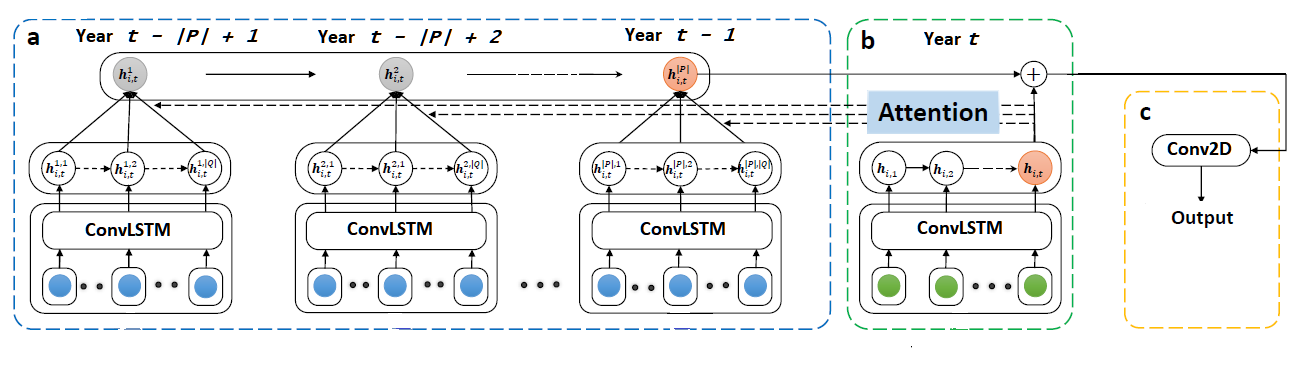
\includegraphics[width=1.0\linewidth]{figures/chap4/A-CLSTM.png}
    \caption{The architecture of A-CLSTM.}{The architecture of A-CLSTM. (a) Periodically shifted attention mechanism captures the long-term periodic dependency and temporal shifting. (b) The short-term temporal dependency is captured by ConvLSTM layer(s). (c) Joint Training to combine outputs of (a) and (b).}
    \label{fig:chap4-architecture-A-CLSTM}
\end{figure}
For simplifying symbols, we set batch size $B = 1$ and ignore it in the following description (see Figure \ref{fig:chap4-architecture-A-CLSTM}).

\textbf{Short-Term Temporal Dependency:}

The first input, \textit{short-term CNN feature} $X1$, is fed into list $C1$ consisted of $SL$ $3 \times 3$ convolution layers with 64 filters. Then each image $X1_i$ convolves with the convolution layer $C1_i$ to generate a list of tensors with shape $(H, W, 64)$. These tensors are then concatenated to produce a tensor with shape $(SL, H, W, 64)$, which is called \textit{short-term-cnn-feature}.

The second input, \textit{short-term LSTM feature} $X2$, whose shape is $(SL, H, W, FH + FL)$, is concatenated with the output of the previous step, \textit{short-term-cnn-feature}, along the last axis to output a tensor \textit{short-term-concat} with shape $(SL, H, W, FH + FL + 64)$. Then this output tensor is passed to a ConvLSTM layer(s) to capture the spatial temporal relationship in the short-term context. Note that the number 64 can be substitute by any integer number, depending on the property of our data. The purpose of these two parts is gathering more information from the nearest previous data, because of their close relevance with the target image. Moreover, the additional information from further past isn't used in the manner of extending the input sequence length as usual, but is used to extend the channel dimension. It plays an important role in making used of the annually periodic property of the hydrological data. Then the latent representation of the short-term part is computed by:
\[ h_t = RNN(\mbox{\textit{short-term-concat}}_t, h_{t-1}), \label{equation-short-term-information}\]
where $RNN$ is ConvLSTM layer(s). $h_t$ then has the shape $(H, W, F1)$, where $F1$ is the filter size of the last used ConvLSTM layer to compute \eqref{equation-short-term-information}. 

\textbf{Periodically Shifted Attention Mechanism:}

The third input, \textit{long-term CNN feature} $X3$ with shape $(P, Q, H, W)$, is handled in the similar way as \textit{short-term CNN feature}, but with the convolutional filter 32, to produce a tensor \textit{long-term-cnn-feature} with shape $(P, Q, H, W, 32)$. 

The fourth input, \textit{long-term LSTM feature} $X4$ with shape $(P, Q, H, W, FH + FL)$, is concatenated with \textit{long-term-cnn-feature} along the channel axis to output a tensor with shape $(P, Q, H, W, FH + FL + 32)$ which is called \textit{long-term-concat}. Similar to \textit{short-term LSTM feature}, the number 32 can be modified as appropriate. Then for each period with index $p$ in $P$, ConvLSTM layer(s) is used to capture the hidden representation of each the relevant time in each period $\mbox{\textit{long-term-concat}}_p$. 

\[ h_t^{p, q} = RNN(\mbox{\textit{long-term-concat}}_t^{p, q}, h_t^{p, q - 1}), \label{equation-long-term-information} \]
where $h_t^{p, q}$ is the representation of time $q$ in previous year $p$ for the predicted time $t$.

By using an attention mechanism, we capture the periodic property of the range of timesteps relevant to timesteps $t$ in period $p$ by computing the weighted sum of all $h_t^{p, q}$ (\eqref{equation:attension-general}) in period $p$ ($h_t^{p, 0}$, $h_t^{p, 1}$,\dots,$h_t^{p, q-1}$).
\[ h_t^p = \sum_{q \in Q}{\alpha_t^{p,q} h_t^{p,q}}, \label{equation:attension-general} \]
where weight $\alpha_t^{p,q}$ indicates how much the value of $h_t^{p,q}$ contributes to the value of $h_t^p$. A way to compute $\alpha_t^{p,q}$ is computing the softmax of score indicating the similarity between the previous hidden state $h_t^{p,q}$ and the short-term information $h_t$ (\eqref{equation-short-term-information}). Let $score(h_t^{p,q}, h_t)$ be the selected similarity, the following function is adopted to compute $score$: \cite{DBLP:journals/corr/LuongPM15}
\[ score(h_t^{p,q}, h_t) = v^T\tanh(W_H h_t^{p,q} + W_X h_t + b_X), \]
where $W_H, W_X, b_X \mbox{ and } v$ are learnable parameters, $v^T$ denotes the transpose of $v$. Then $\alpha_t^{p,q}$ is formulated as:
\[ \alpha_t^{p,q} = \frac{\exp(score(h_t^{p,q}, h_t))}{\sum_{q \in Q}{\exp(score(h_t^{p,q}, h_t))}}. \]
For each previous period $p$, we get the periodic representation $h_t^p$ by \eqref{equation:attension-general}. After that, we adopt another ConvLSTM layer(s) to summary the long-term periodic information:
\[ \hat{h}_t^p = RNN(h_t^p, \hat{h}_t^{p-1}) \]
The last time $\hat{h}_t^P$ represents the periodic property of temporal data in a shape of $(H, W, F2)$, where $F2$ is the filter size of the last used ConvLSTM layer to compute $\hat{h}_t^P$.

\textbf{Joint Training:}
Long-term periodic information $\hat{h}_t^P$ and short-term information $h_t$ are concatenated along the channel axis to produce $h_t^c$ which includes both long-term and short-term spatial temporal data. Notice that $h_t^c$ has the shape of $(H, W, F1 + F2)$. Finally, a 2D convolution layer with kernel size 3 and filter 1 is applied on $h_t^c$ to receive the final prediction $\hat{X}_{t+1}$.
\[ \hat{X}_{t+1} = Conv2D(h_t^c) \]

\textbf{Loss Function:} We use L2 loss to train and monitor the validation. 

\section{Experiments}
We compare the performance of our method with ConvLSTM and with a new method in video prediction, PredRNN++ \cite{wang2018predrnn}. 

\subsection{Experimental Settings}
\subsubsection{Data Preprocessing and Data Augmentation}
First we download all MODIS Terra and Aqua in Tonle Sap lake region from 26/6/2002 to 31/12/2017 (subsection \ref{subsection-used-data}). Then, before generating four inputs for each target image from timesteps $t_0 = (FH + P)*S + Q/2$, we extract band NDVI of these images. The fill value of band NDVI is substituted from -3000 to -2001 to increase the continuity of data (see here\footnote{\url{https://lpdaac.usgs.gov/products/mod13q1v006/}} and here\footnote{\url{https://lpdaac.usgs.gov/products/myd13q1v006/}} for more information of MOD13Q1 and MYD13Q1 data). Then we concatenate these NDVI data in the order of time and then scale them to range $[0,1]$ by min-max normalization (min and max value are min and max of data from 2002 to 2015, corresponding to the range of training data). After that we have a tensor of NDVI data with shape $(714 \times 513 \times 513)$. The threshold for classifying a pixel to be water or not is now:
\[(0.1 - (-0.2001)) / (1.0 -(-0.2001)) \approx 0.2500624947921007
\] 

\subsubsection{Implementation Details}
We implement our method with Tensorflow 1.12 \cite{tensorflow2015-whitepaper}. For training the model, we used Adam \cite{article:Adam-optimization} with the mini-batch of 8 inputs. The training was done in a machine equipped with Intel Xeon E5-2650, 377GB RAM, one Nvidia Tesla P100 and CUDA 9.0. In training and validation phase, we choose patch training strategy in order to increase the amount of training data and speed up training time (we only extract patches whose centers lie on the lake's boundary. For more information of how patches are extracted, see section \ref{Supplementary}). The selected patch size is \textit{32}, in order to speed up training process while also guaranteeing the spatial structure of satellite image data. When testing, we adopt and evaluate our model by two different approaches: inferencing model on whole image data or inferencing model on patches on a grid and combining them to yield the final predicted image. For simplicity, we abbreviate these two approaches as $A-CLSTM$ and $A-CLSTM-G32$ respectively according to inferencing on whole images or on patches.  

\subsubsection{Baselines}
For comparison, we completed the following baseline models:
\begin{itemize}
    \item \textbf{ConvLSTM}: We use four stacked ConvLSTM layers with filter sizes 128, 64, 64, 1 respectively.
    \item \textbf{PredRNN++}: We use PredRNN++ with all hyperparameters mentioned in the paper \cite{wang2018predrnn}.
\end{itemize}

\subsection{Evaluation measures}
\begin{itemize}
    \item \textbf{Mean Squared Error (MSE)} that is the mean squared error of predicted and groundtruth image. It is also the loss function when training our model.
    \item \textbf{Structural Similarity (SSIM)} \cite{Wang:2004:IQA:2319031.2320551} that is used for measuring the similarity between two images.
    \item \textbf{Normalized Root Mean Squared Error of Predicted Water area ($W\_NRMSE$)} that is the division of $W\_RMSE$ and mean of water area array of images in the test set, where $W\_RMSE$ is calculated by: first we extract mask of lake's water pixel of 2D groundtruth and predicted image (see algorithms described in section \ref{Supplementary}); then we obtain the total number of water pixels of these two images by counting the number of 1-value elements of each mask; and last, water area is derived by product of the number of the water pixels and $0.25^2 km^2$ (pixel size of a MODIS Terra/Aqua image data). $W\_RMSE$ is the root mean squared error between groundtruth and predicted water area arrays.
\end{itemize}
The following three metrics are commonly-used metrics in classification problems. Especially, the two latter are more robust on imbalanced classification problems, which is more suitable for the problem in this chapter \footnotetext{By using a simple counting, we notice that the number of lake's water pixels only takes about 17\% in the total pixels of an image.}.
All of these metrics are computed by flatten groundtruth and predicted image (or sequence of images, in term of multiple steps prediction) into two 1D arrays, then apply these metrics' formula to archive scores. In experiments, we use \texttt{sklearn.metrics} module of Scikit-learn library \cite{scikit-learn}. These metrics are defined as:
\begin{itemize}
    \item \textbf{F1-Score} that is harmomic mean of precision and recall.
    \item \textbf{Area under the Precision-Recall Curve (PR-AUC)} that summarizes a precision-recall curve as the weighted mean of precisions achieved at each threshold, with the increase in recall from the previous threshold used as the weight:
    \[ \texttt{PR-AUC} = \sum_n{(R_n - R_{n-1})}{P_n}, \]
    where $P_n$ and $R_n$ are the precision and recall at the nth threshold. PR-AUC is a better metric for our goal given that the dataset is class-imbalanced \cite{article:precision-recall-plot}.
    \item \textbf{Receiver Operating Characteristic (ROC)} Another implementation to approximate Area Under the Precsion-Recall Curve.
\end{itemize}

\subsection{Results}

\begin{table}[h]\footnotesize
    \centering
    \begin{tabular}{|c|c|c|c|c|c|}
    \hline
    \textbf{Metrics}               & \textbf{\begin{tabular}[c]{@{}c@{}}Steps\\ Predict\end{tabular}} & \textbf{ConvLSTM}                                                   & \textbf{PredRNN++}                                                  & \textbf{A-CLSTM}                                          & \textbf{A-CLSTM-G32}                                              \\ \hline
    \multirow{4}{*}{\textbf{MSE}}  & 1                                                                & \textbf{\begin{tabular}[c]{@{}c@{}}0.0105\\  (0.0073)\end{tabular}} & \textbf{\begin{tabular}[c]{@{}c@{}}0.0103 \\ (0.0072)\end{tabular}} & \begin{tabular}[c]{@{}c@{}}0.0152\\  (0.0065)\end{tabular} & \begin{tabular}[c]{@{}c@{}}0.0111 \\ (0.0074)\end{tabular}          \\ \cline{2-6} 
                                   & 3                                                                & \textbf{\begin{tabular}[c]{@{}c@{}}0.0109 \\ (0.0067)\end{tabular}} & \textbf{\begin{tabular}[c]{@{}c@{}}0.011\\  (0.0066)\end{tabular}}  & \begin{tabular}[c]{@{}c@{}}0.0238 \\ (0.0084)\end{tabular} & \begin{tabular}[c]{@{}c@{}}0.0116 \\ (0.0063)\end{tabular}          \\ \cline{2-6} 
                                   & 10                                                               & \textbf{\begin{tabular}[c]{@{}c@{}}0.0152 \\ (0.0062)\end{tabular}} & \begin{tabular}[c]{@{}c@{}}0.0176 \\ (0.0067)\end{tabular}          & \begin{tabular}[c]{@{}c@{}}0.0476 \\ (0.0135)\end{tabular} & \textbf{\begin{tabular}[c]{@{}c@{}}0.0161 \\ (0.0053)\end{tabular}} \\ \cline{2-6} 
                                   & 20                                                               & \textbf{\begin{tabular}[c]{@{}c@{}}0.0174 \\ (0.0041)\end{tabular}} & \begin{tabular}[c]{@{}c@{}}0.022 \\ (0.0054)\end{tabular}           & \begin{tabular}[c]{@{}c@{}}0.0582 \\ (0.0129)\end{tabular} & \textbf{\begin{tabular}[c]{@{}c@{}}0.0187 \\ (0.004)\end{tabular}}  \\ \hline
    \multirow{4}{*}{\textbf{SSIM}} & 1                                                                & \textbf{\begin{tabular}[c]{@{}c@{}}0.5912 \\ (0.1352)\end{tabular}} & \textbf{\begin{tabular}[c]{@{}c@{}}0.5835\\  (0.1369)\end{tabular}} & \begin{tabular}[c]{@{}c@{}}0.5418 \\ (0.1368)\end{tabular} & \begin{tabular}[c]{@{}c@{}}0.5625 \\ (0.1281)\end{tabular}          \\ \cline{2-6} 
                                   & 3                                                                & \textbf{\begin{tabular}[c]{@{}c@{}}0.59 \\ (0.1191)\end{tabular}}   & \textbf{\begin{tabular}[c]{@{}c@{}}0.5754\\  (0.1223)\end{tabular}} & \begin{tabular}[c]{@{}c@{}}0.5127\\  (0.121)\end{tabular}  & \begin{tabular}[c]{@{}c@{}}0.5488 \\ (0.1078)\end{tabular}          \\ \cline{2-6} 
                                   & 10                                                               & \textbf{\begin{tabular}[c]{@{}c@{}}0.523 \\ (0.0932)\end{tabular}}  & \textbf{\begin{tabular}[c]{@{}c@{}}0.4869 \\ (0.1044)\end{tabular}} & \begin{tabular}[c]{@{}c@{}}0.3869 \\ (0.0972)\end{tabular} & \begin{tabular}[c]{@{}c@{}}0.4583 \\ (0.0812)\end{tabular}          \\ \cline{2-6} 
                                   & 20                                                               & \textbf{\begin{tabular}[c]{@{}c@{}}0.4849 \\ (0.0592)\end{tabular}} & \textbf{\begin{tabular}[c]{@{}c@{}}0.4347 \\ (0.0739)\end{tabular}} & \begin{tabular}[c]{@{}c@{}}0.3162 \\ (0.0709)\end{tabular} & \begin{tabular}[c]{@{}c@{}}0.4027 \\ (0.0534)\end{tabular}          \\ \hline
    \end{tabular}
    \caption{Tonle Sap lake hydrological prediction performance in term of regression metrics. With regard to SSIM, higher score is better. Otherwise, lower MSE shows a better performance.}
    \label{tab:chap4-regression-metrics}
\end{table}


\begin{table}[h]\footnotesize
    \centering
    \begin{tabular}{|c|c|c|c|c|c|}
    \hline
    \textbf{Metrics}                    & \textbf{\begin{tabular}[c]{@{}c@{}}Steps \\ Predict\end{tabular}} & \textbf{ConvLSTM}                                                   & \textbf{PredRNN++}                                         & \textbf{A-CLSTM}                                                   & \textbf{A-CLSTM-G32}                                              \\ \hline
    \multirow{4}{*}{\textbf{W\_NRMSE}}  & 1                                                                 & \begin{tabular}[c]{@{}c@{}}0.0138 \\ (0.0158)\end{tabular}          & \begin{tabular}[c]{@{}c@{}}0.0137\\  (0.0148)\end{tabular} & \textbf{\begin{tabular}[c]{@{}c@{}}0.0103 \\ (0.0129)\end{tabular}} & \textbf{\begin{tabular}[c]{@{}c@{}}0.0118 \\ (0.0141)\end{tabular}} \\ \cline{2-6} 
                                        & 3                                                                 & \begin{tabular}[c]{@{}c@{}}0.015 \\ (0.0158)\end{tabular}           & \begin{tabular}[c]{@{}c@{}}0.0217 \\ (0.0171)\end{tabular} & \textbf{\begin{tabular}[c]{@{}c@{}}0.0099 \\ (0.0073)\end{tabular}} & \textbf{\begin{tabular}[c]{@{}c@{}}0.0102 \\ (0.0093)\end{tabular}} \\ \cline{2-6} 
                                        & 10                                                                & \begin{tabular}[c]{@{}c@{}}0.0233 \\ (0.0187)\end{tabular}          & \begin{tabular}[c]{@{}c@{}}0.0473 \\ (0.0262)\end{tabular} & \textbf{\begin{tabular}[c]{@{}c@{}}0.0195 \\ (0.0134)\end{tabular}} & \textbf{\begin{tabular}[c]{@{}c@{}}0.0143 \\ (0.0118)\end{tabular}} \\ \cline{2-6} 
                                        & 20                                                                & \textbf{\begin{tabular}[c]{@{}c@{}}0.0315 \\ (0.0167)\end{tabular}} & \begin{tabular}[c]{@{}c@{}}0.0699 \\ (0.0302)\end{tabular} & \begin{tabular}[c]{@{}c@{}}0.0345 \\ (0.0248)\end{tabular}          & \textbf{\begin{tabular}[c]{@{}c@{}}0.0216 \\ (0.0181)\end{tabular}} \\ \hline
    \multirow{4}{*}{\textbf{F1-Score}} & 1                                                                 & \begin{tabular}[c]{@{}c@{}}0.987 \\ (0.0095)\end{tabular}           & \begin{tabular}[c]{@{}c@{}}0.9867 \\ (0.0089)\end{tabular} & \textbf{\begin{tabular}[c]{@{}c@{}}0.9872 \\ (0.009)\end{tabular}}  & \textbf{\begin{tabular}[c]{@{}c@{}}0.987\\  (0.0089)\end{tabular}}  \\ \cline{2-6} 
                                        & 3                                                                 & \begin{tabular}[c]{@{}c@{}}0.9872 \\ (0.0093)\end{tabular}          & \begin{tabular}[c]{@{}c@{}}0.9848\\  (0.0091)\end{tabular} & \textbf{\begin{tabular}[c]{@{}c@{}}0.9872\\  (0.0087)\end{tabular}} & \textbf{\begin{tabular}[c]{@{}c@{}}0.9877 \\ (0.0081)\end{tabular}} \\ \cline{2-6} 
                                        & 10                                                                & \textbf{\begin{tabular}[c]{@{}c@{}}0.9831 \\ (0.0099)\end{tabular}} & \begin{tabular}[c]{@{}c@{}}0.9732 \\ (0.0127)\end{tabular} & \begin{tabular}[c]{@{}c@{}}0.9789 \\ (0.0142)\end{tabular}          & \textbf{\begin{tabular}[c]{@{}c@{}}0.9845 \\ (0.009)\end{tabular}}  \\ \cline{2-6} 
                                        & 20                                                                & \textbf{\begin{tabular}[c]{@{}c@{}}0.9786 \\ (0.0079)\end{tabular}} & \begin{tabular}[c]{@{}c@{}}0.9623 \\ (0.0145)\end{tabular} & \begin{tabular}[c]{@{}c@{}}0.9662 \\ (0.0204)\end{tabular}          & \textbf{\begin{tabular}[c]{@{}c@{}}0.9803\\  (0.0089)\end{tabular}} \\ \hline
    \multirow{4}{*}{\textbf{ROC-AUC}}  & 1                                                                 & \begin{tabular}[c]{@{}c@{}}0.9906 \\ (0.0086)\end{tabular}          & \begin{tabular}[c]{@{}c@{}}0.9897\\  (0.0077)\end{tabular} & \textbf{\begin{tabular}[c]{@{}c@{}}0.9916 \\ (0.0072)\end{tabular}} & \textbf{\begin{tabular}[c]{@{}c@{}}0.9907 \\ (0.0077)\end{tabular}} \\ \cline{2-6} 
                                        & 3                                                                 & \begin{tabular}[c]{@{}c@{}}0.9909 \\ (0.009)\end{tabular}           & \begin{tabular}[c]{@{}c@{}}0.9869 \\ (0.0085)\end{tabular} & \textbf{\begin{tabular}[c]{@{}c@{}}0.9923 \\ (0.0067)\end{tabular}} & \textbf{\begin{tabular}[c]{@{}c@{}}0.9917 \\ (0.0065)\end{tabular}} \\ \cline{2-6} 
                                        & 10                                                                & \begin{tabular}[c]{@{}c@{}}0.9878 \\ (0.0106)\end{tabular}          & \begin{tabular}[c]{@{}c@{}}0.9751\\  (0.0119)\end{tabular} & \textbf{\begin{tabular}[c]{@{}c@{}}0.9882 \\ (0.0099)\end{tabular}} & \textbf{\begin{tabular}[c]{@{}c@{}}0.9891 \\ (0.0074)\end{tabular}} \\ \cline{2-6} 
                                        & 20                                                                & \textbf{\begin{tabular}[c]{@{}c@{}}0.984 \\ (0.0098)\end{tabular}}  & \begin{tabular}[c]{@{}c@{}}0.9648 \\ (0.0134)\end{tabular} & \begin{tabular}[c]{@{}c@{}}0.981 \\ (0.0139)\end{tabular}           & \textbf{\begin{tabular}[c]{@{}c@{}}0.9851 \\ (0.0086)\end{tabular}} \\ \hline
    \multirow{4}{*}{\textbf{PR-AUC}}   & 1                                                                 & \textbf{\begin{tabular}[c]{@{}c@{}}0.9773 \\ (0.0156)\end{tabular}} & \begin{tabular}[c]{@{}c@{}}0.9772 \\ (0.0147)\end{tabular} & \begin{tabular}[c]{@{}c@{}}0.9772 \\ (0.0155)\end{tabular}          & \textbf{\begin{tabular}[c]{@{}c@{}}0.9773 \\ (0.0148)\end{tabular}} \\ \cline{2-6} 
                                        & 3                                                                 & \textbf{\begin{tabular}[c]{@{}c@{}}0.9777 \\ (0.0148)\end{tabular}} & \begin{tabular}[c]{@{}c@{}}0.9745 \\ (0.0145)\end{tabular} & \begin{tabular}[c]{@{}c@{}}0.9769 \\ (0.015)\end{tabular}           & \textbf{\begin{tabular}[c]{@{}c@{}}0.9782 \\ (0.0138)\end{tabular}} \\ \cline{2-6} 
                                        & 10                                                                & \textbf{\begin{tabular}[c]{@{}c@{}}0.9707 \\ (0.0153)\end{tabular}} & \begin{tabular}[c]{@{}c@{}}0.9568\\  (0.0192)\end{tabular} & \begin{tabular}[c]{@{}c@{}}0.962\\  (0.0243)\end{tabular}           & \textbf{\begin{tabular}[c]{@{}c@{}}0.9729 \\ (0.015)\end{tabular}}  \\ \cline{2-6} 
                                        & 20                                                                & \textbf{\begin{tabular}[c]{@{}c@{}}0.9637 \\ (0.0113)\end{tabular}} & \begin{tabular}[c]{@{}c@{}}0.9406 \\ (0.0213)\end{tabular} & \begin{tabular}[c]{@{}c@{}}0.9405 \\ (0.0341)\end{tabular}          & \textbf{\begin{tabular}[c]{@{}c@{}}0.9664 \\ (0.0139)\end{tabular}} \\ \hline
    \end{tabular}
    \caption{Tonle Sap lake hydrological prediction performance in term of classification metrics. With regard to  W\_NRMSE, lower score is better. Otherwise, higher F1-Score, ROC-AUC and PR-AUC show a better performance.}
    \label{tab:chap4-classification-metrics}
\end{table}

We evaluate the prediction performance of all models in both term of regression and classification. The regression results are reported in Table \ref{tab:chap4-regression-metrics} and classification results are reported in Table \ref{tab:chap4-classification-metrics}. In each row of these two tables, we bold the two best metric values to emphasize the comparisons. Numbers outside and inside parentheses of both tables are metric's mean and metric's standard deviation on the test set, respectively. 

Table \ref{tab:chap4-regression-metrics} shows that our methods yield a higher loss and lower structural similarity than the traditional ConvLSTM model. PredRNN++ performs better in short-term prediction, and its results decrease dramatically when the number of prediction steps increases. The under-expected regression score of the whole-image inference approach (A-CLSTM) and a comparable regression score of A-CLSTM-G32 indicate that applying attention mechanism only on the channel axis cannot guarantee the performance when the input tensors in testing phase have different shape with those in the training data. 

In contrast with the low regression scores, as we see in Table \ref{tab:chap4-classification-metrics}, our methods, especially A-CLSTM-G32, perform better in classification metrics than traditional RNN methods. The difference of classification metrics across multiple methods lies principally on the neighbor region of the lake's boundary, rather than the lake's permanent water region and the far outside lake's region. The better performance of our methods demonstrates that they are more suitable for lake's hydrological prediction, which is the primary goal of this work.

The dramatic decreasing in almost all metrics of PredRNN++ across number of predicted steps indicates that it isn't suitable for capturing long-term temporal property of hydrological data. A-CLSTM-G32 archives the first rank at almost all cases, and always in the top two best performance, shows that A-CLSTM-G32 can properly capture the temporal classification of lake's shoreline region. Figure \ref{fig:metrics-comparisons-timesteps-1} and \ref{fig:metrics-comparisons-timesteps-2} show mean of metrics of each predicted image at each timesteps (metric values in Table \ref{tab:chap4-regression-metrics} and Table \ref{tab:chap4-classification-metrics} are mean across all timesteps in one prediction). We can see that A-CLSTM-G32 performs better than others in all four metrics: W\_NRMSE,  F1-Score, PR-AUC and ROC-AUC at almost all timesteps, which demonstrates a prospective ability of A-CLSTM-G32 in lake's water body prediction problem.

\begin{figure}[h!]
    \begin{center}
    \begin{tabular}[b]{c}
      %% Creator: Matplotlib, PGF backend
%%
%% To include the figure in your LaTeX document, write
%%   \input{<filename>.pgf}
%%
%% Make sure the required packages are loaded in your preamble
%%   \usepackage{pgf}
%%
%% Figures using additional raster images can only be included by \input if
%% they are in the same directory as the main LaTeX file. For loading figures
%% from other directories you can use the `import` package
%%   \usepackage{import}
%% and then include the figures with
%%   \import{<path to file>}{<filename>.pgf}
%%
%% Matplotlib used the following preamble
%%   \usepackage{fontspec}
%%   \setmainfont{DejaVuSerif.ttf}[Path=/usr/local/lib/python3.6/dist-packages/matplotlib/mpl-data/fonts/ttf/]
%%   \setsansfont{DejaVuSans.ttf}[Path=/usr/local/lib/python3.6/dist-packages/matplotlib/mpl-data/fonts/ttf/]
%%   \setmonofont{DejaVuSansMono.ttf}[Path=/usr/local/lib/python3.6/dist-packages/matplotlib/mpl-data/fonts/ttf/]
%%
\begingroup%
\makeatletter%
\begin{pgfpicture}%
\pgfpathrectangle{\pgfpointorigin}{\pgfqpoint{4.000000in}{2.472136in}}%
\pgfusepath{use as bounding box, clip}%
\begin{pgfscope}%
\pgfsetbuttcap%
\pgfsetmiterjoin%
\definecolor{currentfill}{rgb}{1.000000,1.000000,1.000000}%
\pgfsetfillcolor{currentfill}%
\pgfsetlinewidth{0.000000pt}%
\definecolor{currentstroke}{rgb}{1.000000,1.000000,1.000000}%
\pgfsetstrokecolor{currentstroke}%
\pgfsetdash{}{0pt}%
\pgfpathmoveto{\pgfqpoint{0.000000in}{0.000000in}}%
\pgfpathlineto{\pgfqpoint{4.000000in}{0.000000in}}%
\pgfpathlineto{\pgfqpoint{4.000000in}{2.472136in}}%
\pgfpathlineto{\pgfqpoint{0.000000in}{2.472136in}}%
\pgfpathclose%
\pgfusepath{fill}%
\end{pgfscope}%
\begin{pgfscope}%
\pgfsetbuttcap%
\pgfsetmiterjoin%
\definecolor{currentfill}{rgb}{1.000000,1.000000,1.000000}%
\pgfsetfillcolor{currentfill}%
\pgfsetlinewidth{0.000000pt}%
\definecolor{currentstroke}{rgb}{0.000000,0.000000,0.000000}%
\pgfsetstrokecolor{currentstroke}%
\pgfsetstrokeopacity{0.000000}%
\pgfsetdash{}{0pt}%
\pgfpathmoveto{\pgfqpoint{0.671765in}{0.548769in}}%
\pgfpathlineto{\pgfqpoint{3.850000in}{0.548769in}}%
\pgfpathlineto{\pgfqpoint{3.850000in}{2.322136in}}%
\pgfpathlineto{\pgfqpoint{0.671765in}{2.322136in}}%
\pgfpathclose%
\pgfusepath{fill}%
\end{pgfscope}%
\begin{pgfscope}%
\pgfpathrectangle{\pgfqpoint{0.671765in}{0.548769in}}{\pgfqpoint{3.178235in}{1.773367in}}%
\pgfusepath{clip}%
\pgfsetrectcap%
\pgfsetroundjoin%
\pgfsetlinewidth{0.803000pt}%
\definecolor{currentstroke}{rgb}{0.690196,0.690196,0.690196}%
\pgfsetstrokecolor{currentstroke}%
\pgfsetdash{}{0pt}%
\pgfpathmoveto{\pgfqpoint{0.816230in}{0.548769in}}%
\pgfpathlineto{\pgfqpoint{0.816230in}{2.322136in}}%
\pgfusepath{stroke}%
\end{pgfscope}%
\begin{pgfscope}%
\pgfsetbuttcap%
\pgfsetroundjoin%
\definecolor{currentfill}{rgb}{0.501961,0.501961,0.501961}%
\pgfsetfillcolor{currentfill}%
\pgfsetlinewidth{0.803000pt}%
\definecolor{currentstroke}{rgb}{0.501961,0.501961,0.501961}%
\pgfsetstrokecolor{currentstroke}%
\pgfsetdash{}{0pt}%
\pgfsys@defobject{currentmarker}{\pgfqpoint{0.000000in}{-0.048611in}}{\pgfqpoint{0.000000in}{0.000000in}}{%
\pgfpathmoveto{\pgfqpoint{0.000000in}{0.000000in}}%
\pgfpathlineto{\pgfqpoint{0.000000in}{-0.048611in}}%
\pgfusepath{stroke,fill}%
}%
\begin{pgfscope}%
\pgfsys@transformshift{0.816230in}{0.548769in}%
\pgfsys@useobject{currentmarker}{}%
\end{pgfscope}%
\end{pgfscope}%
\begin{pgfscope}%
\definecolor{textcolor}{rgb}{0.000000,0.000000,0.000000}%
\pgfsetstrokecolor{textcolor}%
\pgfsetfillcolor{textcolor}%
\pgftext[x=0.816230in,y=0.451547in,,top]{\color{textcolor}\rmfamily\fontsize{10.000000}{12.000000}\selectfont 1}%
\end{pgfscope}%
\begin{pgfscope}%
\pgfpathrectangle{\pgfqpoint{0.671765in}{0.548769in}}{\pgfqpoint{3.178235in}{1.773367in}}%
\pgfusepath{clip}%
\pgfsetrectcap%
\pgfsetroundjoin%
\pgfsetlinewidth{0.803000pt}%
\definecolor{currentstroke}{rgb}{0.690196,0.690196,0.690196}%
\pgfsetstrokecolor{currentstroke}%
\pgfsetdash{}{0pt}%
\pgfpathmoveto{\pgfqpoint{1.120368in}{0.548769in}}%
\pgfpathlineto{\pgfqpoint{1.120368in}{2.322136in}}%
\pgfusepath{stroke}%
\end{pgfscope}%
\begin{pgfscope}%
\pgfsetbuttcap%
\pgfsetroundjoin%
\definecolor{currentfill}{rgb}{0.501961,0.501961,0.501961}%
\pgfsetfillcolor{currentfill}%
\pgfsetlinewidth{0.803000pt}%
\definecolor{currentstroke}{rgb}{0.501961,0.501961,0.501961}%
\pgfsetstrokecolor{currentstroke}%
\pgfsetdash{}{0pt}%
\pgfsys@defobject{currentmarker}{\pgfqpoint{0.000000in}{-0.048611in}}{\pgfqpoint{0.000000in}{0.000000in}}{%
\pgfpathmoveto{\pgfqpoint{0.000000in}{0.000000in}}%
\pgfpathlineto{\pgfqpoint{0.000000in}{-0.048611in}}%
\pgfusepath{stroke,fill}%
}%
\begin{pgfscope}%
\pgfsys@transformshift{1.120368in}{0.548769in}%
\pgfsys@useobject{currentmarker}{}%
\end{pgfscope}%
\end{pgfscope}%
\begin{pgfscope}%
\definecolor{textcolor}{rgb}{0.000000,0.000000,0.000000}%
\pgfsetstrokecolor{textcolor}%
\pgfsetfillcolor{textcolor}%
\pgftext[x=1.120368in,y=0.451547in,,top]{\color{textcolor}\rmfamily\fontsize{10.000000}{12.000000}\selectfont 3}%
\end{pgfscope}%
\begin{pgfscope}%
\pgfpathrectangle{\pgfqpoint{0.671765in}{0.548769in}}{\pgfqpoint{3.178235in}{1.773367in}}%
\pgfusepath{clip}%
\pgfsetrectcap%
\pgfsetroundjoin%
\pgfsetlinewidth{0.803000pt}%
\definecolor{currentstroke}{rgb}{0.690196,0.690196,0.690196}%
\pgfsetstrokecolor{currentstroke}%
\pgfsetdash{}{0pt}%
\pgfpathmoveto{\pgfqpoint{1.424505in}{0.548769in}}%
\pgfpathlineto{\pgfqpoint{1.424505in}{2.322136in}}%
\pgfusepath{stroke}%
\end{pgfscope}%
\begin{pgfscope}%
\pgfsetbuttcap%
\pgfsetroundjoin%
\definecolor{currentfill}{rgb}{0.501961,0.501961,0.501961}%
\pgfsetfillcolor{currentfill}%
\pgfsetlinewidth{0.803000pt}%
\definecolor{currentstroke}{rgb}{0.501961,0.501961,0.501961}%
\pgfsetstrokecolor{currentstroke}%
\pgfsetdash{}{0pt}%
\pgfsys@defobject{currentmarker}{\pgfqpoint{0.000000in}{-0.048611in}}{\pgfqpoint{0.000000in}{0.000000in}}{%
\pgfpathmoveto{\pgfqpoint{0.000000in}{0.000000in}}%
\pgfpathlineto{\pgfqpoint{0.000000in}{-0.048611in}}%
\pgfusepath{stroke,fill}%
}%
\begin{pgfscope}%
\pgfsys@transformshift{1.424505in}{0.548769in}%
\pgfsys@useobject{currentmarker}{}%
\end{pgfscope}%
\end{pgfscope}%
\begin{pgfscope}%
\definecolor{textcolor}{rgb}{0.000000,0.000000,0.000000}%
\pgfsetstrokecolor{textcolor}%
\pgfsetfillcolor{textcolor}%
\pgftext[x=1.424505in,y=0.451547in,,top]{\color{textcolor}\rmfamily\fontsize{10.000000}{12.000000}\selectfont 5}%
\end{pgfscope}%
\begin{pgfscope}%
\pgfpathrectangle{\pgfqpoint{0.671765in}{0.548769in}}{\pgfqpoint{3.178235in}{1.773367in}}%
\pgfusepath{clip}%
\pgfsetrectcap%
\pgfsetroundjoin%
\pgfsetlinewidth{0.803000pt}%
\definecolor{currentstroke}{rgb}{0.690196,0.690196,0.690196}%
\pgfsetstrokecolor{currentstroke}%
\pgfsetdash{}{0pt}%
\pgfpathmoveto{\pgfqpoint{1.728642in}{0.548769in}}%
\pgfpathlineto{\pgfqpoint{1.728642in}{2.322136in}}%
\pgfusepath{stroke}%
\end{pgfscope}%
\begin{pgfscope}%
\pgfsetbuttcap%
\pgfsetroundjoin%
\definecolor{currentfill}{rgb}{0.501961,0.501961,0.501961}%
\pgfsetfillcolor{currentfill}%
\pgfsetlinewidth{0.803000pt}%
\definecolor{currentstroke}{rgb}{0.501961,0.501961,0.501961}%
\pgfsetstrokecolor{currentstroke}%
\pgfsetdash{}{0pt}%
\pgfsys@defobject{currentmarker}{\pgfqpoint{0.000000in}{-0.048611in}}{\pgfqpoint{0.000000in}{0.000000in}}{%
\pgfpathmoveto{\pgfqpoint{0.000000in}{0.000000in}}%
\pgfpathlineto{\pgfqpoint{0.000000in}{-0.048611in}}%
\pgfusepath{stroke,fill}%
}%
\begin{pgfscope}%
\pgfsys@transformshift{1.728642in}{0.548769in}%
\pgfsys@useobject{currentmarker}{}%
\end{pgfscope}%
\end{pgfscope}%
\begin{pgfscope}%
\definecolor{textcolor}{rgb}{0.000000,0.000000,0.000000}%
\pgfsetstrokecolor{textcolor}%
\pgfsetfillcolor{textcolor}%
\pgftext[x=1.728642in,y=0.451547in,,top]{\color{textcolor}\rmfamily\fontsize{10.000000}{12.000000}\selectfont 7}%
\end{pgfscope}%
\begin{pgfscope}%
\pgfpathrectangle{\pgfqpoint{0.671765in}{0.548769in}}{\pgfqpoint{3.178235in}{1.773367in}}%
\pgfusepath{clip}%
\pgfsetrectcap%
\pgfsetroundjoin%
\pgfsetlinewidth{0.803000pt}%
\definecolor{currentstroke}{rgb}{0.690196,0.690196,0.690196}%
\pgfsetstrokecolor{currentstroke}%
\pgfsetdash{}{0pt}%
\pgfpathmoveto{\pgfqpoint{2.032780in}{0.548769in}}%
\pgfpathlineto{\pgfqpoint{2.032780in}{2.322136in}}%
\pgfusepath{stroke}%
\end{pgfscope}%
\begin{pgfscope}%
\pgfsetbuttcap%
\pgfsetroundjoin%
\definecolor{currentfill}{rgb}{0.501961,0.501961,0.501961}%
\pgfsetfillcolor{currentfill}%
\pgfsetlinewidth{0.803000pt}%
\definecolor{currentstroke}{rgb}{0.501961,0.501961,0.501961}%
\pgfsetstrokecolor{currentstroke}%
\pgfsetdash{}{0pt}%
\pgfsys@defobject{currentmarker}{\pgfqpoint{0.000000in}{-0.048611in}}{\pgfqpoint{0.000000in}{0.000000in}}{%
\pgfpathmoveto{\pgfqpoint{0.000000in}{0.000000in}}%
\pgfpathlineto{\pgfqpoint{0.000000in}{-0.048611in}}%
\pgfusepath{stroke,fill}%
}%
\begin{pgfscope}%
\pgfsys@transformshift{2.032780in}{0.548769in}%
\pgfsys@useobject{currentmarker}{}%
\end{pgfscope}%
\end{pgfscope}%
\begin{pgfscope}%
\definecolor{textcolor}{rgb}{0.000000,0.000000,0.000000}%
\pgfsetstrokecolor{textcolor}%
\pgfsetfillcolor{textcolor}%
\pgftext[x=2.032780in,y=0.451547in,,top]{\color{textcolor}\rmfamily\fontsize{10.000000}{12.000000}\selectfont 9}%
\end{pgfscope}%
\begin{pgfscope}%
\pgfpathrectangle{\pgfqpoint{0.671765in}{0.548769in}}{\pgfqpoint{3.178235in}{1.773367in}}%
\pgfusepath{clip}%
\pgfsetrectcap%
\pgfsetroundjoin%
\pgfsetlinewidth{0.803000pt}%
\definecolor{currentstroke}{rgb}{0.690196,0.690196,0.690196}%
\pgfsetstrokecolor{currentstroke}%
\pgfsetdash{}{0pt}%
\pgfpathmoveto{\pgfqpoint{2.336917in}{0.548769in}}%
\pgfpathlineto{\pgfqpoint{2.336917in}{2.322136in}}%
\pgfusepath{stroke}%
\end{pgfscope}%
\begin{pgfscope}%
\pgfsetbuttcap%
\pgfsetroundjoin%
\definecolor{currentfill}{rgb}{0.501961,0.501961,0.501961}%
\pgfsetfillcolor{currentfill}%
\pgfsetlinewidth{0.803000pt}%
\definecolor{currentstroke}{rgb}{0.501961,0.501961,0.501961}%
\pgfsetstrokecolor{currentstroke}%
\pgfsetdash{}{0pt}%
\pgfsys@defobject{currentmarker}{\pgfqpoint{0.000000in}{-0.048611in}}{\pgfqpoint{0.000000in}{0.000000in}}{%
\pgfpathmoveto{\pgfqpoint{0.000000in}{0.000000in}}%
\pgfpathlineto{\pgfqpoint{0.000000in}{-0.048611in}}%
\pgfusepath{stroke,fill}%
}%
\begin{pgfscope}%
\pgfsys@transformshift{2.336917in}{0.548769in}%
\pgfsys@useobject{currentmarker}{}%
\end{pgfscope}%
\end{pgfscope}%
\begin{pgfscope}%
\definecolor{textcolor}{rgb}{0.000000,0.000000,0.000000}%
\pgfsetstrokecolor{textcolor}%
\pgfsetfillcolor{textcolor}%
\pgftext[x=2.336917in,y=0.451547in,,top]{\color{textcolor}\rmfamily\fontsize{10.000000}{12.000000}\selectfont 11}%
\end{pgfscope}%
\begin{pgfscope}%
\pgfpathrectangle{\pgfqpoint{0.671765in}{0.548769in}}{\pgfqpoint{3.178235in}{1.773367in}}%
\pgfusepath{clip}%
\pgfsetrectcap%
\pgfsetroundjoin%
\pgfsetlinewidth{0.803000pt}%
\definecolor{currentstroke}{rgb}{0.690196,0.690196,0.690196}%
\pgfsetstrokecolor{currentstroke}%
\pgfsetdash{}{0pt}%
\pgfpathmoveto{\pgfqpoint{2.641054in}{0.548769in}}%
\pgfpathlineto{\pgfqpoint{2.641054in}{2.322136in}}%
\pgfusepath{stroke}%
\end{pgfscope}%
\begin{pgfscope}%
\pgfsetbuttcap%
\pgfsetroundjoin%
\definecolor{currentfill}{rgb}{0.501961,0.501961,0.501961}%
\pgfsetfillcolor{currentfill}%
\pgfsetlinewidth{0.803000pt}%
\definecolor{currentstroke}{rgb}{0.501961,0.501961,0.501961}%
\pgfsetstrokecolor{currentstroke}%
\pgfsetdash{}{0pt}%
\pgfsys@defobject{currentmarker}{\pgfqpoint{0.000000in}{-0.048611in}}{\pgfqpoint{0.000000in}{0.000000in}}{%
\pgfpathmoveto{\pgfqpoint{0.000000in}{0.000000in}}%
\pgfpathlineto{\pgfqpoint{0.000000in}{-0.048611in}}%
\pgfusepath{stroke,fill}%
}%
\begin{pgfscope}%
\pgfsys@transformshift{2.641054in}{0.548769in}%
\pgfsys@useobject{currentmarker}{}%
\end{pgfscope}%
\end{pgfscope}%
\begin{pgfscope}%
\definecolor{textcolor}{rgb}{0.000000,0.000000,0.000000}%
\pgfsetstrokecolor{textcolor}%
\pgfsetfillcolor{textcolor}%
\pgftext[x=2.641054in,y=0.451547in,,top]{\color{textcolor}\rmfamily\fontsize{10.000000}{12.000000}\selectfont 13}%
\end{pgfscope}%
\begin{pgfscope}%
\pgfpathrectangle{\pgfqpoint{0.671765in}{0.548769in}}{\pgfqpoint{3.178235in}{1.773367in}}%
\pgfusepath{clip}%
\pgfsetrectcap%
\pgfsetroundjoin%
\pgfsetlinewidth{0.803000pt}%
\definecolor{currentstroke}{rgb}{0.690196,0.690196,0.690196}%
\pgfsetstrokecolor{currentstroke}%
\pgfsetdash{}{0pt}%
\pgfpathmoveto{\pgfqpoint{2.945192in}{0.548769in}}%
\pgfpathlineto{\pgfqpoint{2.945192in}{2.322136in}}%
\pgfusepath{stroke}%
\end{pgfscope}%
\begin{pgfscope}%
\pgfsetbuttcap%
\pgfsetroundjoin%
\definecolor{currentfill}{rgb}{0.501961,0.501961,0.501961}%
\pgfsetfillcolor{currentfill}%
\pgfsetlinewidth{0.803000pt}%
\definecolor{currentstroke}{rgb}{0.501961,0.501961,0.501961}%
\pgfsetstrokecolor{currentstroke}%
\pgfsetdash{}{0pt}%
\pgfsys@defobject{currentmarker}{\pgfqpoint{0.000000in}{-0.048611in}}{\pgfqpoint{0.000000in}{0.000000in}}{%
\pgfpathmoveto{\pgfqpoint{0.000000in}{0.000000in}}%
\pgfpathlineto{\pgfqpoint{0.000000in}{-0.048611in}}%
\pgfusepath{stroke,fill}%
}%
\begin{pgfscope}%
\pgfsys@transformshift{2.945192in}{0.548769in}%
\pgfsys@useobject{currentmarker}{}%
\end{pgfscope}%
\end{pgfscope}%
\begin{pgfscope}%
\definecolor{textcolor}{rgb}{0.000000,0.000000,0.000000}%
\pgfsetstrokecolor{textcolor}%
\pgfsetfillcolor{textcolor}%
\pgftext[x=2.945192in,y=0.451547in,,top]{\color{textcolor}\rmfamily\fontsize{10.000000}{12.000000}\selectfont 15}%
\end{pgfscope}%
\begin{pgfscope}%
\pgfpathrectangle{\pgfqpoint{0.671765in}{0.548769in}}{\pgfqpoint{3.178235in}{1.773367in}}%
\pgfusepath{clip}%
\pgfsetrectcap%
\pgfsetroundjoin%
\pgfsetlinewidth{0.803000pt}%
\definecolor{currentstroke}{rgb}{0.690196,0.690196,0.690196}%
\pgfsetstrokecolor{currentstroke}%
\pgfsetdash{}{0pt}%
\pgfpathmoveto{\pgfqpoint{3.249329in}{0.548769in}}%
\pgfpathlineto{\pgfqpoint{3.249329in}{2.322136in}}%
\pgfusepath{stroke}%
\end{pgfscope}%
\begin{pgfscope}%
\pgfsetbuttcap%
\pgfsetroundjoin%
\definecolor{currentfill}{rgb}{0.501961,0.501961,0.501961}%
\pgfsetfillcolor{currentfill}%
\pgfsetlinewidth{0.803000pt}%
\definecolor{currentstroke}{rgb}{0.501961,0.501961,0.501961}%
\pgfsetstrokecolor{currentstroke}%
\pgfsetdash{}{0pt}%
\pgfsys@defobject{currentmarker}{\pgfqpoint{0.000000in}{-0.048611in}}{\pgfqpoint{0.000000in}{0.000000in}}{%
\pgfpathmoveto{\pgfqpoint{0.000000in}{0.000000in}}%
\pgfpathlineto{\pgfqpoint{0.000000in}{-0.048611in}}%
\pgfusepath{stroke,fill}%
}%
\begin{pgfscope}%
\pgfsys@transformshift{3.249329in}{0.548769in}%
\pgfsys@useobject{currentmarker}{}%
\end{pgfscope}%
\end{pgfscope}%
\begin{pgfscope}%
\definecolor{textcolor}{rgb}{0.000000,0.000000,0.000000}%
\pgfsetstrokecolor{textcolor}%
\pgfsetfillcolor{textcolor}%
\pgftext[x=3.249329in,y=0.451547in,,top]{\color{textcolor}\rmfamily\fontsize{10.000000}{12.000000}\selectfont 17}%
\end{pgfscope}%
\begin{pgfscope}%
\pgfpathrectangle{\pgfqpoint{0.671765in}{0.548769in}}{\pgfqpoint{3.178235in}{1.773367in}}%
\pgfusepath{clip}%
\pgfsetrectcap%
\pgfsetroundjoin%
\pgfsetlinewidth{0.803000pt}%
\definecolor{currentstroke}{rgb}{0.690196,0.690196,0.690196}%
\pgfsetstrokecolor{currentstroke}%
\pgfsetdash{}{0pt}%
\pgfpathmoveto{\pgfqpoint{3.553466in}{0.548769in}}%
\pgfpathlineto{\pgfqpoint{3.553466in}{2.322136in}}%
\pgfusepath{stroke}%
\end{pgfscope}%
\begin{pgfscope}%
\pgfsetbuttcap%
\pgfsetroundjoin%
\definecolor{currentfill}{rgb}{0.501961,0.501961,0.501961}%
\pgfsetfillcolor{currentfill}%
\pgfsetlinewidth{0.803000pt}%
\definecolor{currentstroke}{rgb}{0.501961,0.501961,0.501961}%
\pgfsetstrokecolor{currentstroke}%
\pgfsetdash{}{0pt}%
\pgfsys@defobject{currentmarker}{\pgfqpoint{0.000000in}{-0.048611in}}{\pgfqpoint{0.000000in}{0.000000in}}{%
\pgfpathmoveto{\pgfqpoint{0.000000in}{0.000000in}}%
\pgfpathlineto{\pgfqpoint{0.000000in}{-0.048611in}}%
\pgfusepath{stroke,fill}%
}%
\begin{pgfscope}%
\pgfsys@transformshift{3.553466in}{0.548769in}%
\pgfsys@useobject{currentmarker}{}%
\end{pgfscope}%
\end{pgfscope}%
\begin{pgfscope}%
\definecolor{textcolor}{rgb}{0.000000,0.000000,0.000000}%
\pgfsetstrokecolor{textcolor}%
\pgfsetfillcolor{textcolor}%
\pgftext[x=3.553466in,y=0.451547in,,top]{\color{textcolor}\rmfamily\fontsize{10.000000}{12.000000}\selectfont 19}%
\end{pgfscope}%
\begin{pgfscope}%
\definecolor{textcolor}{rgb}{0.000000,0.000000,0.000000}%
\pgfsetstrokecolor{textcolor}%
\pgfsetfillcolor{textcolor}%
\pgftext[x=2.260883in,y=0.261578in,,top]{\color{textcolor}\rmfamily\fontsize{10.000000}{12.000000}\selectfont Steps Prediction}%
\end{pgfscope}%
\begin{pgfscope}%
\pgfpathrectangle{\pgfqpoint{0.671765in}{0.548769in}}{\pgfqpoint{3.178235in}{1.773367in}}%
\pgfusepath{clip}%
\pgfsetrectcap%
\pgfsetroundjoin%
\pgfsetlinewidth{0.803000pt}%
\definecolor{currentstroke}{rgb}{0.690196,0.690196,0.690196}%
\pgfsetstrokecolor{currentstroke}%
\pgfsetdash{}{0pt}%
\pgfpathmoveto{\pgfqpoint{0.671765in}{0.800905in}}%
\pgfpathlineto{\pgfqpoint{3.850000in}{0.800905in}}%
\pgfusepath{stroke}%
\end{pgfscope}%
\begin{pgfscope}%
\pgfsetbuttcap%
\pgfsetroundjoin%
\definecolor{currentfill}{rgb}{0.501961,0.501961,0.501961}%
\pgfsetfillcolor{currentfill}%
\pgfsetlinewidth{0.803000pt}%
\definecolor{currentstroke}{rgb}{0.501961,0.501961,0.501961}%
\pgfsetstrokecolor{currentstroke}%
\pgfsetdash{}{0pt}%
\pgfsys@defobject{currentmarker}{\pgfqpoint{-0.048611in}{0.000000in}}{\pgfqpoint{0.000000in}{0.000000in}}{%
\pgfpathmoveto{\pgfqpoint{0.000000in}{0.000000in}}%
\pgfpathlineto{\pgfqpoint{-0.048611in}{0.000000in}}%
\pgfusepath{stroke,fill}%
}%
\begin{pgfscope}%
\pgfsys@transformshift{0.671765in}{0.800905in}%
\pgfsys@useobject{currentmarker}{}%
\end{pgfscope}%
\end{pgfscope}%
\begin{pgfscope}%
\definecolor{textcolor}{rgb}{0.000000,0.000000,0.000000}%
\pgfsetstrokecolor{textcolor}%
\pgfsetfillcolor{textcolor}%
\pgftext[x=0.327629in,y=0.748143in,left,base]{\color{textcolor}\rmfamily\fontsize{10.000000}{12.000000}\selectfont \(\displaystyle 0.02\)}%
\end{pgfscope}%
\begin{pgfscope}%
\pgfpathrectangle{\pgfqpoint{0.671765in}{0.548769in}}{\pgfqpoint{3.178235in}{1.773367in}}%
\pgfusepath{clip}%
\pgfsetrectcap%
\pgfsetroundjoin%
\pgfsetlinewidth{0.803000pt}%
\definecolor{currentstroke}{rgb}{0.690196,0.690196,0.690196}%
\pgfsetstrokecolor{currentstroke}%
\pgfsetdash{}{0pt}%
\pgfpathmoveto{\pgfqpoint{0.671765in}{1.146923in}}%
\pgfpathlineto{\pgfqpoint{3.850000in}{1.146923in}}%
\pgfusepath{stroke}%
\end{pgfscope}%
\begin{pgfscope}%
\pgfsetbuttcap%
\pgfsetroundjoin%
\definecolor{currentfill}{rgb}{0.501961,0.501961,0.501961}%
\pgfsetfillcolor{currentfill}%
\pgfsetlinewidth{0.803000pt}%
\definecolor{currentstroke}{rgb}{0.501961,0.501961,0.501961}%
\pgfsetstrokecolor{currentstroke}%
\pgfsetdash{}{0pt}%
\pgfsys@defobject{currentmarker}{\pgfqpoint{-0.048611in}{0.000000in}}{\pgfqpoint{0.000000in}{0.000000in}}{%
\pgfpathmoveto{\pgfqpoint{0.000000in}{0.000000in}}%
\pgfpathlineto{\pgfqpoint{-0.048611in}{0.000000in}}%
\pgfusepath{stroke,fill}%
}%
\begin{pgfscope}%
\pgfsys@transformshift{0.671765in}{1.146923in}%
\pgfsys@useobject{currentmarker}{}%
\end{pgfscope}%
\end{pgfscope}%
\begin{pgfscope}%
\definecolor{textcolor}{rgb}{0.000000,0.000000,0.000000}%
\pgfsetstrokecolor{textcolor}%
\pgfsetfillcolor{textcolor}%
\pgftext[x=0.327629in,y=1.094161in,left,base]{\color{textcolor}\rmfamily\fontsize{10.000000}{12.000000}\selectfont \(\displaystyle 0.04\)}%
\end{pgfscope}%
\begin{pgfscope}%
\pgfpathrectangle{\pgfqpoint{0.671765in}{0.548769in}}{\pgfqpoint{3.178235in}{1.773367in}}%
\pgfusepath{clip}%
\pgfsetrectcap%
\pgfsetroundjoin%
\pgfsetlinewidth{0.803000pt}%
\definecolor{currentstroke}{rgb}{0.690196,0.690196,0.690196}%
\pgfsetstrokecolor{currentstroke}%
\pgfsetdash{}{0pt}%
\pgfpathmoveto{\pgfqpoint{0.671765in}{1.492941in}}%
\pgfpathlineto{\pgfqpoint{3.850000in}{1.492941in}}%
\pgfusepath{stroke}%
\end{pgfscope}%
\begin{pgfscope}%
\pgfsetbuttcap%
\pgfsetroundjoin%
\definecolor{currentfill}{rgb}{0.501961,0.501961,0.501961}%
\pgfsetfillcolor{currentfill}%
\pgfsetlinewidth{0.803000pt}%
\definecolor{currentstroke}{rgb}{0.501961,0.501961,0.501961}%
\pgfsetstrokecolor{currentstroke}%
\pgfsetdash{}{0pt}%
\pgfsys@defobject{currentmarker}{\pgfqpoint{-0.048611in}{0.000000in}}{\pgfqpoint{0.000000in}{0.000000in}}{%
\pgfpathmoveto{\pgfqpoint{0.000000in}{0.000000in}}%
\pgfpathlineto{\pgfqpoint{-0.048611in}{0.000000in}}%
\pgfusepath{stroke,fill}%
}%
\begin{pgfscope}%
\pgfsys@transformshift{0.671765in}{1.492941in}%
\pgfsys@useobject{currentmarker}{}%
\end{pgfscope}%
\end{pgfscope}%
\begin{pgfscope}%
\definecolor{textcolor}{rgb}{0.000000,0.000000,0.000000}%
\pgfsetstrokecolor{textcolor}%
\pgfsetfillcolor{textcolor}%
\pgftext[x=0.327629in,y=1.440179in,left,base]{\color{textcolor}\rmfamily\fontsize{10.000000}{12.000000}\selectfont \(\displaystyle 0.06\)}%
\end{pgfscope}%
\begin{pgfscope}%
\pgfpathrectangle{\pgfqpoint{0.671765in}{0.548769in}}{\pgfqpoint{3.178235in}{1.773367in}}%
\pgfusepath{clip}%
\pgfsetrectcap%
\pgfsetroundjoin%
\pgfsetlinewidth{0.803000pt}%
\definecolor{currentstroke}{rgb}{0.690196,0.690196,0.690196}%
\pgfsetstrokecolor{currentstroke}%
\pgfsetdash{}{0pt}%
\pgfpathmoveto{\pgfqpoint{0.671765in}{1.838959in}}%
\pgfpathlineto{\pgfqpoint{3.850000in}{1.838959in}}%
\pgfusepath{stroke}%
\end{pgfscope}%
\begin{pgfscope}%
\pgfsetbuttcap%
\pgfsetroundjoin%
\definecolor{currentfill}{rgb}{0.501961,0.501961,0.501961}%
\pgfsetfillcolor{currentfill}%
\pgfsetlinewidth{0.803000pt}%
\definecolor{currentstroke}{rgb}{0.501961,0.501961,0.501961}%
\pgfsetstrokecolor{currentstroke}%
\pgfsetdash{}{0pt}%
\pgfsys@defobject{currentmarker}{\pgfqpoint{-0.048611in}{0.000000in}}{\pgfqpoint{0.000000in}{0.000000in}}{%
\pgfpathmoveto{\pgfqpoint{0.000000in}{0.000000in}}%
\pgfpathlineto{\pgfqpoint{-0.048611in}{0.000000in}}%
\pgfusepath{stroke,fill}%
}%
\begin{pgfscope}%
\pgfsys@transformshift{0.671765in}{1.838959in}%
\pgfsys@useobject{currentmarker}{}%
\end{pgfscope}%
\end{pgfscope}%
\begin{pgfscope}%
\definecolor{textcolor}{rgb}{0.000000,0.000000,0.000000}%
\pgfsetstrokecolor{textcolor}%
\pgfsetfillcolor{textcolor}%
\pgftext[x=0.327629in,y=1.786197in,left,base]{\color{textcolor}\rmfamily\fontsize{10.000000}{12.000000}\selectfont \(\displaystyle 0.08\)}%
\end{pgfscope}%
\begin{pgfscope}%
\pgfpathrectangle{\pgfqpoint{0.671765in}{0.548769in}}{\pgfqpoint{3.178235in}{1.773367in}}%
\pgfusepath{clip}%
\pgfsetrectcap%
\pgfsetroundjoin%
\pgfsetlinewidth{0.803000pt}%
\definecolor{currentstroke}{rgb}{0.690196,0.690196,0.690196}%
\pgfsetstrokecolor{currentstroke}%
\pgfsetdash{}{0pt}%
\pgfpathmoveto{\pgfqpoint{0.671765in}{2.184977in}}%
\pgfpathlineto{\pgfqpoint{3.850000in}{2.184977in}}%
\pgfusepath{stroke}%
\end{pgfscope}%
\begin{pgfscope}%
\pgfsetbuttcap%
\pgfsetroundjoin%
\definecolor{currentfill}{rgb}{0.501961,0.501961,0.501961}%
\pgfsetfillcolor{currentfill}%
\pgfsetlinewidth{0.803000pt}%
\definecolor{currentstroke}{rgb}{0.501961,0.501961,0.501961}%
\pgfsetstrokecolor{currentstroke}%
\pgfsetdash{}{0pt}%
\pgfsys@defobject{currentmarker}{\pgfqpoint{-0.048611in}{0.000000in}}{\pgfqpoint{0.000000in}{0.000000in}}{%
\pgfpathmoveto{\pgfqpoint{0.000000in}{0.000000in}}%
\pgfpathlineto{\pgfqpoint{-0.048611in}{0.000000in}}%
\pgfusepath{stroke,fill}%
}%
\begin{pgfscope}%
\pgfsys@transformshift{0.671765in}{2.184977in}%
\pgfsys@useobject{currentmarker}{}%
\end{pgfscope}%
\end{pgfscope}%
\begin{pgfscope}%
\definecolor{textcolor}{rgb}{0.000000,0.000000,0.000000}%
\pgfsetstrokecolor{textcolor}%
\pgfsetfillcolor{textcolor}%
\pgftext[x=0.327629in,y=2.132215in,left,base]{\color{textcolor}\rmfamily\fontsize{10.000000}{12.000000}\selectfont \(\displaystyle 0.10\)}%
\end{pgfscope}%
\begin{pgfscope}%
\definecolor{textcolor}{rgb}{0.000000,0.000000,0.000000}%
\pgfsetstrokecolor{textcolor}%
\pgfsetfillcolor{textcolor}%
\pgftext[x=0.272073in,y=1.435452in,,bottom,rotate=90.000000]{\color{textcolor}\rmfamily\fontsize{10.000000}{12.000000}\selectfont Mean of Water-NRMSE}%
\end{pgfscope}%
\begin{pgfscope}%
\pgfpathrectangle{\pgfqpoint{0.671765in}{0.548769in}}{\pgfqpoint{3.178235in}{1.773367in}}%
\pgfusepath{clip}%
\pgfsetrectcap%
\pgfsetroundjoin%
\pgfsetlinewidth{1.505625pt}%
\definecolor{currentstroke}{rgb}{1.000000,0.000000,0.000000}%
\pgfsetstrokecolor{currentstroke}%
\pgfsetdash{}{0pt}%
\pgfpathmoveto{\pgfqpoint{0.816230in}{0.694212in}}%
\pgfpathlineto{\pgfqpoint{0.968299in}{0.726335in}}%
\pgfpathlineto{\pgfqpoint{1.120368in}{0.772574in}}%
\pgfpathlineto{\pgfqpoint{1.272436in}{0.815754in}}%
\pgfpathlineto{\pgfqpoint{1.424505in}{0.858295in}}%
\pgfpathlineto{\pgfqpoint{1.576574in}{0.891152in}}%
\pgfpathlineto{\pgfqpoint{1.728642in}{0.914332in}}%
\pgfpathlineto{\pgfqpoint{1.880711in}{0.947028in}}%
\pgfpathlineto{\pgfqpoint{2.032780in}{0.980046in}}%
\pgfpathlineto{\pgfqpoint{2.184848in}{1.024648in}}%
\pgfpathlineto{\pgfqpoint{2.336917in}{1.074041in}}%
\pgfpathlineto{\pgfqpoint{2.488986in}{1.119570in}}%
\pgfpathlineto{\pgfqpoint{2.641054in}{1.143364in}}%
\pgfpathlineto{\pgfqpoint{2.793123in}{1.148460in}}%
\pgfpathlineto{\pgfqpoint{2.945192in}{1.151955in}}%
\pgfpathlineto{\pgfqpoint{3.097260in}{1.150856in}}%
\pgfpathlineto{\pgfqpoint{3.249329in}{1.151728in}}%
\pgfpathlineto{\pgfqpoint{3.401397in}{1.165122in}}%
\pgfpathlineto{\pgfqpoint{3.553466in}{1.165982in}}%
\pgfpathlineto{\pgfqpoint{3.705535in}{1.162081in}}%
\pgfusepath{stroke}%
\end{pgfscope}%
\begin{pgfscope}%
\pgfpathrectangle{\pgfqpoint{0.671765in}{0.548769in}}{\pgfqpoint{3.178235in}{1.773367in}}%
\pgfusepath{clip}%
\pgfsetbuttcap%
\pgfsetroundjoin%
\definecolor{currentfill}{rgb}{1.000000,0.000000,0.000000}%
\pgfsetfillcolor{currentfill}%
\pgfsetlinewidth{1.003750pt}%
\definecolor{currentstroke}{rgb}{1.000000,0.000000,0.000000}%
\pgfsetstrokecolor{currentstroke}%
\pgfsetdash{}{0pt}%
\pgfsys@defobject{currentmarker}{\pgfqpoint{-0.041667in}{-0.041667in}}{\pgfqpoint{0.041667in}{0.041667in}}{%
\pgfpathmoveto{\pgfqpoint{0.000000in}{-0.041667in}}%
\pgfpathcurveto{\pgfqpoint{0.011050in}{-0.041667in}}{\pgfqpoint{0.021649in}{-0.037276in}}{\pgfqpoint{0.029463in}{-0.029463in}}%
\pgfpathcurveto{\pgfqpoint{0.037276in}{-0.021649in}}{\pgfqpoint{0.041667in}{-0.011050in}}{\pgfqpoint{0.041667in}{0.000000in}}%
\pgfpathcurveto{\pgfqpoint{0.041667in}{0.011050in}}{\pgfqpoint{0.037276in}{0.021649in}}{\pgfqpoint{0.029463in}{0.029463in}}%
\pgfpathcurveto{\pgfqpoint{0.021649in}{0.037276in}}{\pgfqpoint{0.011050in}{0.041667in}}{\pgfqpoint{0.000000in}{0.041667in}}%
\pgfpathcurveto{\pgfqpoint{-0.011050in}{0.041667in}}{\pgfqpoint{-0.021649in}{0.037276in}}{\pgfqpoint{-0.029463in}{0.029463in}}%
\pgfpathcurveto{\pgfqpoint{-0.037276in}{0.021649in}}{\pgfqpoint{-0.041667in}{0.011050in}}{\pgfqpoint{-0.041667in}{0.000000in}}%
\pgfpathcurveto{\pgfqpoint{-0.041667in}{-0.011050in}}{\pgfqpoint{-0.037276in}{-0.021649in}}{\pgfqpoint{-0.029463in}{-0.029463in}}%
\pgfpathcurveto{\pgfqpoint{-0.021649in}{-0.037276in}}{\pgfqpoint{-0.011050in}{-0.041667in}}{\pgfqpoint{0.000000in}{-0.041667in}}%
\pgfpathclose%
\pgfusepath{stroke,fill}%
}%
\begin{pgfscope}%
\pgfsys@transformshift{0.816230in}{0.694212in}%
\pgfsys@useobject{currentmarker}{}%
\end{pgfscope}%
\begin{pgfscope}%
\pgfsys@transformshift{0.968299in}{0.726335in}%
\pgfsys@useobject{currentmarker}{}%
\end{pgfscope}%
\begin{pgfscope}%
\pgfsys@transformshift{1.120368in}{0.772574in}%
\pgfsys@useobject{currentmarker}{}%
\end{pgfscope}%
\begin{pgfscope}%
\pgfsys@transformshift{1.272436in}{0.815754in}%
\pgfsys@useobject{currentmarker}{}%
\end{pgfscope}%
\begin{pgfscope}%
\pgfsys@transformshift{1.424505in}{0.858295in}%
\pgfsys@useobject{currentmarker}{}%
\end{pgfscope}%
\begin{pgfscope}%
\pgfsys@transformshift{1.576574in}{0.891152in}%
\pgfsys@useobject{currentmarker}{}%
\end{pgfscope}%
\begin{pgfscope}%
\pgfsys@transformshift{1.728642in}{0.914332in}%
\pgfsys@useobject{currentmarker}{}%
\end{pgfscope}%
\begin{pgfscope}%
\pgfsys@transformshift{1.880711in}{0.947028in}%
\pgfsys@useobject{currentmarker}{}%
\end{pgfscope}%
\begin{pgfscope}%
\pgfsys@transformshift{2.032780in}{0.980046in}%
\pgfsys@useobject{currentmarker}{}%
\end{pgfscope}%
\begin{pgfscope}%
\pgfsys@transformshift{2.184848in}{1.024648in}%
\pgfsys@useobject{currentmarker}{}%
\end{pgfscope}%
\begin{pgfscope}%
\pgfsys@transformshift{2.336917in}{1.074041in}%
\pgfsys@useobject{currentmarker}{}%
\end{pgfscope}%
\begin{pgfscope}%
\pgfsys@transformshift{2.488986in}{1.119570in}%
\pgfsys@useobject{currentmarker}{}%
\end{pgfscope}%
\begin{pgfscope}%
\pgfsys@transformshift{2.641054in}{1.143364in}%
\pgfsys@useobject{currentmarker}{}%
\end{pgfscope}%
\begin{pgfscope}%
\pgfsys@transformshift{2.793123in}{1.148460in}%
\pgfsys@useobject{currentmarker}{}%
\end{pgfscope}%
\begin{pgfscope}%
\pgfsys@transformshift{2.945192in}{1.151955in}%
\pgfsys@useobject{currentmarker}{}%
\end{pgfscope}%
\begin{pgfscope}%
\pgfsys@transformshift{3.097260in}{1.150856in}%
\pgfsys@useobject{currentmarker}{}%
\end{pgfscope}%
\begin{pgfscope}%
\pgfsys@transformshift{3.249329in}{1.151728in}%
\pgfsys@useobject{currentmarker}{}%
\end{pgfscope}%
\begin{pgfscope}%
\pgfsys@transformshift{3.401397in}{1.165122in}%
\pgfsys@useobject{currentmarker}{}%
\end{pgfscope}%
\begin{pgfscope}%
\pgfsys@transformshift{3.553466in}{1.165982in}%
\pgfsys@useobject{currentmarker}{}%
\end{pgfscope}%
\begin{pgfscope}%
\pgfsys@transformshift{3.705535in}{1.162081in}%
\pgfsys@useobject{currentmarker}{}%
\end{pgfscope}%
\end{pgfscope}%
\begin{pgfscope}%
\pgfpathrectangle{\pgfqpoint{0.671765in}{0.548769in}}{\pgfqpoint{3.178235in}{1.773367in}}%
\pgfusepath{clip}%
\pgfsetrectcap%
\pgfsetroundjoin%
\pgfsetlinewidth{1.505625pt}%
\definecolor{currentstroke}{rgb}{0.000000,0.500000,0.000000}%
\pgfsetstrokecolor{currentstroke}%
\pgfsetdash{}{0pt}%
\pgfpathmoveto{\pgfqpoint{0.816230in}{0.691416in}}%
\pgfpathlineto{\pgfqpoint{0.968299in}{0.830367in}}%
\pgfpathlineto{\pgfqpoint{1.120368in}{1.008052in}}%
\pgfpathlineto{\pgfqpoint{1.272436in}{1.155587in}}%
\pgfpathlineto{\pgfqpoint{1.424505in}{1.285654in}}%
\pgfpathlineto{\pgfqpoint{1.576574in}{1.396645in}}%
\pgfpathlineto{\pgfqpoint{1.728642in}{1.481094in}}%
\pgfpathlineto{\pgfqpoint{1.880711in}{1.560226in}}%
\pgfpathlineto{\pgfqpoint{2.032780in}{1.638091in}}%
\pgfpathlineto{\pgfqpoint{2.184848in}{1.724165in}}%
\pgfpathlineto{\pgfqpoint{2.336917in}{1.810084in}}%
\pgfpathlineto{\pgfqpoint{2.488986in}{1.889771in}}%
\pgfpathlineto{\pgfqpoint{2.641054in}{1.954733in}}%
\pgfpathlineto{\pgfqpoint{2.793123in}{2.005100in}}%
\pgfpathlineto{\pgfqpoint{2.945192in}{2.052074in}}%
\pgfpathlineto{\pgfqpoint{3.097260in}{2.089907in}}%
\pgfpathlineto{\pgfqpoint{3.249329in}{2.129073in}}%
\pgfpathlineto{\pgfqpoint{3.401397in}{2.176585in}}%
\pgfpathlineto{\pgfqpoint{3.553466in}{2.212704in}}%
\pgfpathlineto{\pgfqpoint{3.705535in}{2.241528in}}%
\pgfusepath{stroke}%
\end{pgfscope}%
\begin{pgfscope}%
\pgfpathrectangle{\pgfqpoint{0.671765in}{0.548769in}}{\pgfqpoint{3.178235in}{1.773367in}}%
\pgfusepath{clip}%
\pgfsetbuttcap%
\pgfsetroundjoin%
\definecolor{currentfill}{rgb}{0.000000,0.500000,0.000000}%
\pgfsetfillcolor{currentfill}%
\pgfsetlinewidth{1.003750pt}%
\definecolor{currentstroke}{rgb}{0.000000,0.500000,0.000000}%
\pgfsetstrokecolor{currentstroke}%
\pgfsetdash{}{0pt}%
\pgfsys@defobject{currentmarker}{\pgfqpoint{-0.041667in}{-0.041667in}}{\pgfqpoint{0.041667in}{0.041667in}}{%
\pgfpathmoveto{\pgfqpoint{-0.041667in}{-0.041667in}}%
\pgfpathlineto{\pgfqpoint{0.041667in}{0.041667in}}%
\pgfpathmoveto{\pgfqpoint{-0.041667in}{0.041667in}}%
\pgfpathlineto{\pgfqpoint{0.041667in}{-0.041667in}}%
\pgfusepath{stroke,fill}%
}%
\begin{pgfscope}%
\pgfsys@transformshift{0.816230in}{0.691416in}%
\pgfsys@useobject{currentmarker}{}%
\end{pgfscope}%
\begin{pgfscope}%
\pgfsys@transformshift{0.968299in}{0.830367in}%
\pgfsys@useobject{currentmarker}{}%
\end{pgfscope}%
\begin{pgfscope}%
\pgfsys@transformshift{1.120368in}{1.008052in}%
\pgfsys@useobject{currentmarker}{}%
\end{pgfscope}%
\begin{pgfscope}%
\pgfsys@transformshift{1.272436in}{1.155587in}%
\pgfsys@useobject{currentmarker}{}%
\end{pgfscope}%
\begin{pgfscope}%
\pgfsys@transformshift{1.424505in}{1.285654in}%
\pgfsys@useobject{currentmarker}{}%
\end{pgfscope}%
\begin{pgfscope}%
\pgfsys@transformshift{1.576574in}{1.396645in}%
\pgfsys@useobject{currentmarker}{}%
\end{pgfscope}%
\begin{pgfscope}%
\pgfsys@transformshift{1.728642in}{1.481094in}%
\pgfsys@useobject{currentmarker}{}%
\end{pgfscope}%
\begin{pgfscope}%
\pgfsys@transformshift{1.880711in}{1.560226in}%
\pgfsys@useobject{currentmarker}{}%
\end{pgfscope}%
\begin{pgfscope}%
\pgfsys@transformshift{2.032780in}{1.638091in}%
\pgfsys@useobject{currentmarker}{}%
\end{pgfscope}%
\begin{pgfscope}%
\pgfsys@transformshift{2.184848in}{1.724165in}%
\pgfsys@useobject{currentmarker}{}%
\end{pgfscope}%
\begin{pgfscope}%
\pgfsys@transformshift{2.336917in}{1.810084in}%
\pgfsys@useobject{currentmarker}{}%
\end{pgfscope}%
\begin{pgfscope}%
\pgfsys@transformshift{2.488986in}{1.889771in}%
\pgfsys@useobject{currentmarker}{}%
\end{pgfscope}%
\begin{pgfscope}%
\pgfsys@transformshift{2.641054in}{1.954733in}%
\pgfsys@useobject{currentmarker}{}%
\end{pgfscope}%
\begin{pgfscope}%
\pgfsys@transformshift{2.793123in}{2.005100in}%
\pgfsys@useobject{currentmarker}{}%
\end{pgfscope}%
\begin{pgfscope}%
\pgfsys@transformshift{2.945192in}{2.052074in}%
\pgfsys@useobject{currentmarker}{}%
\end{pgfscope}%
\begin{pgfscope}%
\pgfsys@transformshift{3.097260in}{2.089907in}%
\pgfsys@useobject{currentmarker}{}%
\end{pgfscope}%
\begin{pgfscope}%
\pgfsys@transformshift{3.249329in}{2.129073in}%
\pgfsys@useobject{currentmarker}{}%
\end{pgfscope}%
\begin{pgfscope}%
\pgfsys@transformshift{3.401397in}{2.176585in}%
\pgfsys@useobject{currentmarker}{}%
\end{pgfscope}%
\begin{pgfscope}%
\pgfsys@transformshift{3.553466in}{2.212704in}%
\pgfsys@useobject{currentmarker}{}%
\end{pgfscope}%
\begin{pgfscope}%
\pgfsys@transformshift{3.705535in}{2.241528in}%
\pgfsys@useobject{currentmarker}{}%
\end{pgfscope}%
\end{pgfscope}%
\begin{pgfscope}%
\pgfpathrectangle{\pgfqpoint{0.671765in}{0.548769in}}{\pgfqpoint{3.178235in}{1.773367in}}%
\pgfusepath{clip}%
\pgfsetrectcap%
\pgfsetroundjoin%
\pgfsetlinewidth{1.505625pt}%
\definecolor{currentstroke}{rgb}{0.000000,0.000000,1.000000}%
\pgfsetstrokecolor{currentstroke}%
\pgfsetdash{}{0pt}%
\pgfpathmoveto{\pgfqpoint{0.816230in}{0.632964in}}%
\pgfpathlineto{\pgfqpoint{0.968299in}{0.629376in}}%
\pgfpathlineto{\pgfqpoint{1.120368in}{0.671051in}}%
\pgfpathlineto{\pgfqpoint{1.272436in}{0.725994in}}%
\pgfpathlineto{\pgfqpoint{1.424505in}{0.779139in}}%
\pgfpathlineto{\pgfqpoint{1.576574in}{0.834781in}}%
\pgfpathlineto{\pgfqpoint{1.728642in}{0.844722in}}%
\pgfpathlineto{\pgfqpoint{1.880711in}{0.878709in}}%
\pgfpathlineto{\pgfqpoint{2.032780in}{0.964298in}}%
\pgfpathlineto{\pgfqpoint{2.184848in}{1.014044in}}%
\pgfpathlineto{\pgfqpoint{2.336917in}{1.069334in}}%
\pgfpathlineto{\pgfqpoint{2.488986in}{1.130359in}}%
\pgfpathlineto{\pgfqpoint{2.641054in}{1.279494in}}%
\pgfpathlineto{\pgfqpoint{2.793123in}{1.243889in}}%
\pgfpathlineto{\pgfqpoint{2.945192in}{1.339617in}}%
\pgfpathlineto{\pgfqpoint{3.097260in}{1.339342in}}%
\pgfpathlineto{\pgfqpoint{3.249329in}{1.404119in}}%
\pgfpathlineto{\pgfqpoint{3.401397in}{1.405230in}}%
\pgfpathlineto{\pgfqpoint{3.553466in}{1.436743in}}%
\pgfpathlineto{\pgfqpoint{3.705535in}{1.453297in}}%
\pgfusepath{stroke}%
\end{pgfscope}%
\begin{pgfscope}%
\pgfpathrectangle{\pgfqpoint{0.671765in}{0.548769in}}{\pgfqpoint{3.178235in}{1.773367in}}%
\pgfusepath{clip}%
\pgfsetbuttcap%
\pgfsetmiterjoin%
\definecolor{currentfill}{rgb}{0.000000,0.000000,1.000000}%
\pgfsetfillcolor{currentfill}%
\pgfsetlinewidth{1.003750pt}%
\definecolor{currentstroke}{rgb}{0.000000,0.000000,1.000000}%
\pgfsetstrokecolor{currentstroke}%
\pgfsetdash{}{0pt}%
\pgfsys@defobject{currentmarker}{\pgfqpoint{-0.058926in}{-0.058926in}}{\pgfqpoint{0.058926in}{0.058926in}}{%
\pgfpathmoveto{\pgfqpoint{-0.000000in}{-0.058926in}}%
\pgfpathlineto{\pgfqpoint{0.058926in}{0.000000in}}%
\pgfpathlineto{\pgfqpoint{0.000000in}{0.058926in}}%
\pgfpathlineto{\pgfqpoint{-0.058926in}{0.000000in}}%
\pgfpathclose%
\pgfusepath{stroke,fill}%
}%
\begin{pgfscope}%
\pgfsys@transformshift{0.816230in}{0.632964in}%
\pgfsys@useobject{currentmarker}{}%
\end{pgfscope}%
\begin{pgfscope}%
\pgfsys@transformshift{0.968299in}{0.629376in}%
\pgfsys@useobject{currentmarker}{}%
\end{pgfscope}%
\begin{pgfscope}%
\pgfsys@transformshift{1.120368in}{0.671051in}%
\pgfsys@useobject{currentmarker}{}%
\end{pgfscope}%
\begin{pgfscope}%
\pgfsys@transformshift{1.272436in}{0.725994in}%
\pgfsys@useobject{currentmarker}{}%
\end{pgfscope}%
\begin{pgfscope}%
\pgfsys@transformshift{1.424505in}{0.779139in}%
\pgfsys@useobject{currentmarker}{}%
\end{pgfscope}%
\begin{pgfscope}%
\pgfsys@transformshift{1.576574in}{0.834781in}%
\pgfsys@useobject{currentmarker}{}%
\end{pgfscope}%
\begin{pgfscope}%
\pgfsys@transformshift{1.728642in}{0.844722in}%
\pgfsys@useobject{currentmarker}{}%
\end{pgfscope}%
\begin{pgfscope}%
\pgfsys@transformshift{1.880711in}{0.878709in}%
\pgfsys@useobject{currentmarker}{}%
\end{pgfscope}%
\begin{pgfscope}%
\pgfsys@transformshift{2.032780in}{0.964298in}%
\pgfsys@useobject{currentmarker}{}%
\end{pgfscope}%
\begin{pgfscope}%
\pgfsys@transformshift{2.184848in}{1.014044in}%
\pgfsys@useobject{currentmarker}{}%
\end{pgfscope}%
\begin{pgfscope}%
\pgfsys@transformshift{2.336917in}{1.069334in}%
\pgfsys@useobject{currentmarker}{}%
\end{pgfscope}%
\begin{pgfscope}%
\pgfsys@transformshift{2.488986in}{1.130359in}%
\pgfsys@useobject{currentmarker}{}%
\end{pgfscope}%
\begin{pgfscope}%
\pgfsys@transformshift{2.641054in}{1.279494in}%
\pgfsys@useobject{currentmarker}{}%
\end{pgfscope}%
\begin{pgfscope}%
\pgfsys@transformshift{2.793123in}{1.243889in}%
\pgfsys@useobject{currentmarker}{}%
\end{pgfscope}%
\begin{pgfscope}%
\pgfsys@transformshift{2.945192in}{1.339617in}%
\pgfsys@useobject{currentmarker}{}%
\end{pgfscope}%
\begin{pgfscope}%
\pgfsys@transformshift{3.097260in}{1.339342in}%
\pgfsys@useobject{currentmarker}{}%
\end{pgfscope}%
\begin{pgfscope}%
\pgfsys@transformshift{3.249329in}{1.404119in}%
\pgfsys@useobject{currentmarker}{}%
\end{pgfscope}%
\begin{pgfscope}%
\pgfsys@transformshift{3.401397in}{1.405230in}%
\pgfsys@useobject{currentmarker}{}%
\end{pgfscope}%
\begin{pgfscope}%
\pgfsys@transformshift{3.553466in}{1.436743in}%
\pgfsys@useobject{currentmarker}{}%
\end{pgfscope}%
\begin{pgfscope}%
\pgfsys@transformshift{3.705535in}{1.453297in}%
\pgfsys@useobject{currentmarker}{}%
\end{pgfscope}%
\end{pgfscope}%
\begin{pgfscope}%
\pgfpathrectangle{\pgfqpoint{0.671765in}{0.548769in}}{\pgfqpoint{3.178235in}{1.773367in}}%
\pgfusepath{clip}%
\pgfsetrectcap%
\pgfsetroundjoin%
\pgfsetlinewidth{1.505625pt}%
\definecolor{currentstroke}{rgb}{1.000000,1.000000,0.000000}%
\pgfsetstrokecolor{currentstroke}%
\pgfsetdash{}{0pt}%
\pgfpathmoveto{\pgfqpoint{0.816230in}{0.659691in}}%
\pgfpathlineto{\pgfqpoint{0.968299in}{0.637734in}}%
\pgfpathlineto{\pgfqpoint{1.120368in}{0.667550in}}%
\pgfpathlineto{\pgfqpoint{1.272436in}{0.691303in}}%
\pgfpathlineto{\pgfqpoint{1.424505in}{0.716406in}}%
\pgfpathlineto{\pgfqpoint{1.576574in}{0.718838in}}%
\pgfpathlineto{\pgfqpoint{1.728642in}{0.719662in}}%
\pgfpathlineto{\pgfqpoint{1.880711in}{0.729340in}}%
\pgfpathlineto{\pgfqpoint{2.032780in}{0.751509in}}%
\pgfpathlineto{\pgfqpoint{2.184848in}{0.796010in}}%
\pgfpathlineto{\pgfqpoint{2.336917in}{0.841162in}}%
\pgfpathlineto{\pgfqpoint{2.488986in}{0.891702in}}%
\pgfpathlineto{\pgfqpoint{2.641054in}{0.915031in}}%
\pgfpathlineto{\pgfqpoint{2.793123in}{0.932230in}}%
\pgfpathlineto{\pgfqpoint{2.945192in}{0.943730in}}%
\pgfpathlineto{\pgfqpoint{3.097260in}{0.956018in}}%
\pgfpathlineto{\pgfqpoint{3.249329in}{0.975470in}}%
\pgfpathlineto{\pgfqpoint{3.401397in}{1.006648in}}%
\pgfpathlineto{\pgfqpoint{3.553466in}{1.029159in}}%
\pgfpathlineto{\pgfqpoint{3.705535in}{1.050838in}}%
\pgfusepath{stroke}%
\end{pgfscope}%
\begin{pgfscope}%
\pgfpathrectangle{\pgfqpoint{0.671765in}{0.548769in}}{\pgfqpoint{3.178235in}{1.773367in}}%
\pgfusepath{clip}%
\pgfsetbuttcap%
\pgfsetbeveljoin%
\definecolor{currentfill}{rgb}{1.000000,1.000000,0.000000}%
\pgfsetfillcolor{currentfill}%
\pgfsetlinewidth{1.003750pt}%
\definecolor{currentstroke}{rgb}{1.000000,1.000000,0.000000}%
\pgfsetstrokecolor{currentstroke}%
\pgfsetdash{}{0pt}%
\pgfsys@defobject{currentmarker}{\pgfqpoint{-0.039627in}{-0.033709in}}{\pgfqpoint{0.039627in}{0.041667in}}{%
\pgfpathmoveto{\pgfqpoint{0.000000in}{0.041667in}}%
\pgfpathlineto{\pgfqpoint{-0.009355in}{0.012876in}}%
\pgfpathlineto{\pgfqpoint{-0.039627in}{0.012876in}}%
\pgfpathlineto{\pgfqpoint{-0.015136in}{-0.004918in}}%
\pgfpathlineto{\pgfqpoint{-0.024491in}{-0.033709in}}%
\pgfpathlineto{\pgfqpoint{-0.000000in}{-0.015915in}}%
\pgfpathlineto{\pgfqpoint{0.024491in}{-0.033709in}}%
\pgfpathlineto{\pgfqpoint{0.015136in}{-0.004918in}}%
\pgfpathlineto{\pgfqpoint{0.039627in}{0.012876in}}%
\pgfpathlineto{\pgfqpoint{0.009355in}{0.012876in}}%
\pgfpathclose%
\pgfusepath{stroke,fill}%
}%
\begin{pgfscope}%
\pgfsys@transformshift{0.816230in}{0.659691in}%
\pgfsys@useobject{currentmarker}{}%
\end{pgfscope}%
\begin{pgfscope}%
\pgfsys@transformshift{0.968299in}{0.637734in}%
\pgfsys@useobject{currentmarker}{}%
\end{pgfscope}%
\begin{pgfscope}%
\pgfsys@transformshift{1.120368in}{0.667550in}%
\pgfsys@useobject{currentmarker}{}%
\end{pgfscope}%
\begin{pgfscope}%
\pgfsys@transformshift{1.272436in}{0.691303in}%
\pgfsys@useobject{currentmarker}{}%
\end{pgfscope}%
\begin{pgfscope}%
\pgfsys@transformshift{1.424505in}{0.716406in}%
\pgfsys@useobject{currentmarker}{}%
\end{pgfscope}%
\begin{pgfscope}%
\pgfsys@transformshift{1.576574in}{0.718838in}%
\pgfsys@useobject{currentmarker}{}%
\end{pgfscope}%
\begin{pgfscope}%
\pgfsys@transformshift{1.728642in}{0.719662in}%
\pgfsys@useobject{currentmarker}{}%
\end{pgfscope}%
\begin{pgfscope}%
\pgfsys@transformshift{1.880711in}{0.729340in}%
\pgfsys@useobject{currentmarker}{}%
\end{pgfscope}%
\begin{pgfscope}%
\pgfsys@transformshift{2.032780in}{0.751509in}%
\pgfsys@useobject{currentmarker}{}%
\end{pgfscope}%
\begin{pgfscope}%
\pgfsys@transformshift{2.184848in}{0.796010in}%
\pgfsys@useobject{currentmarker}{}%
\end{pgfscope}%
\begin{pgfscope}%
\pgfsys@transformshift{2.336917in}{0.841162in}%
\pgfsys@useobject{currentmarker}{}%
\end{pgfscope}%
\begin{pgfscope}%
\pgfsys@transformshift{2.488986in}{0.891702in}%
\pgfsys@useobject{currentmarker}{}%
\end{pgfscope}%
\begin{pgfscope}%
\pgfsys@transformshift{2.641054in}{0.915031in}%
\pgfsys@useobject{currentmarker}{}%
\end{pgfscope}%
\begin{pgfscope}%
\pgfsys@transformshift{2.793123in}{0.932230in}%
\pgfsys@useobject{currentmarker}{}%
\end{pgfscope}%
\begin{pgfscope}%
\pgfsys@transformshift{2.945192in}{0.943730in}%
\pgfsys@useobject{currentmarker}{}%
\end{pgfscope}%
\begin{pgfscope}%
\pgfsys@transformshift{3.097260in}{0.956018in}%
\pgfsys@useobject{currentmarker}{}%
\end{pgfscope}%
\begin{pgfscope}%
\pgfsys@transformshift{3.249329in}{0.975470in}%
\pgfsys@useobject{currentmarker}{}%
\end{pgfscope}%
\begin{pgfscope}%
\pgfsys@transformshift{3.401397in}{1.006648in}%
\pgfsys@useobject{currentmarker}{}%
\end{pgfscope}%
\begin{pgfscope}%
\pgfsys@transformshift{3.553466in}{1.029159in}%
\pgfsys@useobject{currentmarker}{}%
\end{pgfscope}%
\begin{pgfscope}%
\pgfsys@transformshift{3.705535in}{1.050838in}%
\pgfsys@useobject{currentmarker}{}%
\end{pgfscope}%
\end{pgfscope}%
\begin{pgfscope}%
\pgfsetrectcap%
\pgfsetmiterjoin%
\pgfsetlinewidth{0.501875pt}%
\definecolor{currentstroke}{rgb}{0.501961,0.501961,0.501961}%
\pgfsetstrokecolor{currentstroke}%
\pgfsetdash{}{0pt}%
\pgfpathmoveto{\pgfqpoint{0.671765in}{0.548769in}}%
\pgfpathlineto{\pgfqpoint{0.671765in}{2.322136in}}%
\pgfusepath{stroke}%
\end{pgfscope}%
\begin{pgfscope}%
\pgfsetrectcap%
\pgfsetmiterjoin%
\pgfsetlinewidth{0.501875pt}%
\definecolor{currentstroke}{rgb}{0.501961,0.501961,0.501961}%
\pgfsetstrokecolor{currentstroke}%
\pgfsetdash{}{0pt}%
\pgfpathmoveto{\pgfqpoint{0.671765in}{0.548769in}}%
\pgfpathlineto{\pgfqpoint{3.850000in}{0.548769in}}%
\pgfusepath{stroke}%
\end{pgfscope}%
\begin{pgfscope}%
\pgfsetbuttcap%
\pgfsetmiterjoin%
\definecolor{currentfill}{rgb}{1.000000,1.000000,1.000000}%
\pgfsetfillcolor{currentfill}%
\pgfsetfillopacity{0.800000}%
\pgfsetlinewidth{1.003750pt}%
\definecolor{currentstroke}{rgb}{0.800000,0.800000,0.800000}%
\pgfsetstrokecolor{currentstroke}%
\pgfsetstrokeopacity{0.800000}%
\pgfsetdash{}{0pt}%
\pgfpathmoveto{\pgfqpoint{0.768987in}{1.395596in}}%
\pgfpathlineto{\pgfqpoint{2.223767in}{1.395596in}}%
\pgfpathquadraticcurveto{\pgfqpoint{2.251545in}{1.395596in}}{\pgfqpoint{2.251545in}{1.423374in}}%
\pgfpathlineto{\pgfqpoint{2.251545in}{2.224914in}}%
\pgfpathquadraticcurveto{\pgfqpoint{2.251545in}{2.252692in}}{\pgfqpoint{2.223767in}{2.252692in}}%
\pgfpathlineto{\pgfqpoint{0.768987in}{2.252692in}}%
\pgfpathquadraticcurveto{\pgfqpoint{0.741210in}{2.252692in}}{\pgfqpoint{0.741210in}{2.224914in}}%
\pgfpathlineto{\pgfqpoint{0.741210in}{1.423374in}}%
\pgfpathquadraticcurveto{\pgfqpoint{0.741210in}{1.395596in}}{\pgfqpoint{0.768987in}{1.395596in}}%
\pgfpathclose%
\pgfusepath{stroke,fill}%
\end{pgfscope}%
\begin{pgfscope}%
\pgfsetrectcap%
\pgfsetroundjoin%
\pgfsetlinewidth{1.505625pt}%
\definecolor{currentstroke}{rgb}{1.000000,0.000000,0.000000}%
\pgfsetstrokecolor{currentstroke}%
\pgfsetdash{}{0pt}%
\pgfpathmoveto{\pgfqpoint{0.796765in}{2.140224in}}%
\pgfpathlineto{\pgfqpoint{1.074543in}{2.140224in}}%
\pgfusepath{stroke}%
\end{pgfscope}%
\begin{pgfscope}%
\pgfsetbuttcap%
\pgfsetroundjoin%
\definecolor{currentfill}{rgb}{1.000000,0.000000,0.000000}%
\pgfsetfillcolor{currentfill}%
\pgfsetlinewidth{1.003750pt}%
\definecolor{currentstroke}{rgb}{1.000000,0.000000,0.000000}%
\pgfsetstrokecolor{currentstroke}%
\pgfsetdash{}{0pt}%
\pgfsys@defobject{currentmarker}{\pgfqpoint{-0.041667in}{-0.041667in}}{\pgfqpoint{0.041667in}{0.041667in}}{%
\pgfpathmoveto{\pgfqpoint{0.000000in}{-0.041667in}}%
\pgfpathcurveto{\pgfqpoint{0.011050in}{-0.041667in}}{\pgfqpoint{0.021649in}{-0.037276in}}{\pgfqpoint{0.029463in}{-0.029463in}}%
\pgfpathcurveto{\pgfqpoint{0.037276in}{-0.021649in}}{\pgfqpoint{0.041667in}{-0.011050in}}{\pgfqpoint{0.041667in}{0.000000in}}%
\pgfpathcurveto{\pgfqpoint{0.041667in}{0.011050in}}{\pgfqpoint{0.037276in}{0.021649in}}{\pgfqpoint{0.029463in}{0.029463in}}%
\pgfpathcurveto{\pgfqpoint{0.021649in}{0.037276in}}{\pgfqpoint{0.011050in}{0.041667in}}{\pgfqpoint{0.000000in}{0.041667in}}%
\pgfpathcurveto{\pgfqpoint{-0.011050in}{0.041667in}}{\pgfqpoint{-0.021649in}{0.037276in}}{\pgfqpoint{-0.029463in}{0.029463in}}%
\pgfpathcurveto{\pgfqpoint{-0.037276in}{0.021649in}}{\pgfqpoint{-0.041667in}{0.011050in}}{\pgfqpoint{-0.041667in}{0.000000in}}%
\pgfpathcurveto{\pgfqpoint{-0.041667in}{-0.011050in}}{\pgfqpoint{-0.037276in}{-0.021649in}}{\pgfqpoint{-0.029463in}{-0.029463in}}%
\pgfpathcurveto{\pgfqpoint{-0.021649in}{-0.037276in}}{\pgfqpoint{-0.011050in}{-0.041667in}}{\pgfqpoint{0.000000in}{-0.041667in}}%
\pgfpathclose%
\pgfusepath{stroke,fill}%
}%
\begin{pgfscope}%
\pgfsys@transformshift{0.935654in}{2.140224in}%
\pgfsys@useobject{currentmarker}{}%
\end{pgfscope}%
\end{pgfscope}%
\begin{pgfscope}%
\definecolor{textcolor}{rgb}{0.000000,0.000000,0.000000}%
\pgfsetstrokecolor{textcolor}%
\pgfsetfillcolor{textcolor}%
\pgftext[x=1.185654in,y=2.091613in,left,base]{\color{textcolor}\rmfamily\fontsize{10.000000}{12.000000}\selectfont ConvLSTM}%
\end{pgfscope}%
\begin{pgfscope}%
\pgfsetrectcap%
\pgfsetroundjoin%
\pgfsetlinewidth{1.505625pt}%
\definecolor{currentstroke}{rgb}{0.000000,0.500000,0.000000}%
\pgfsetstrokecolor{currentstroke}%
\pgfsetdash{}{0pt}%
\pgfpathmoveto{\pgfqpoint{0.796765in}{1.936367in}}%
\pgfpathlineto{\pgfqpoint{1.074543in}{1.936367in}}%
\pgfusepath{stroke}%
\end{pgfscope}%
\begin{pgfscope}%
\pgfsetbuttcap%
\pgfsetroundjoin%
\definecolor{currentfill}{rgb}{0.000000,0.500000,0.000000}%
\pgfsetfillcolor{currentfill}%
\pgfsetlinewidth{1.003750pt}%
\definecolor{currentstroke}{rgb}{0.000000,0.500000,0.000000}%
\pgfsetstrokecolor{currentstroke}%
\pgfsetdash{}{0pt}%
\pgfsys@defobject{currentmarker}{\pgfqpoint{-0.041667in}{-0.041667in}}{\pgfqpoint{0.041667in}{0.041667in}}{%
\pgfpathmoveto{\pgfqpoint{-0.041667in}{-0.041667in}}%
\pgfpathlineto{\pgfqpoint{0.041667in}{0.041667in}}%
\pgfpathmoveto{\pgfqpoint{-0.041667in}{0.041667in}}%
\pgfpathlineto{\pgfqpoint{0.041667in}{-0.041667in}}%
\pgfusepath{stroke,fill}%
}%
\begin{pgfscope}%
\pgfsys@transformshift{0.935654in}{1.936367in}%
\pgfsys@useobject{currentmarker}{}%
\end{pgfscope}%
\end{pgfscope}%
\begin{pgfscope}%
\definecolor{textcolor}{rgb}{0.000000,0.000000,0.000000}%
\pgfsetstrokecolor{textcolor}%
\pgfsetfillcolor{textcolor}%
\pgftext[x=1.185654in,y=1.887756in,left,base]{\color{textcolor}\rmfamily\fontsize{10.000000}{12.000000}\selectfont PredRNN++}%
\end{pgfscope}%
\begin{pgfscope}%
\pgfsetrectcap%
\pgfsetroundjoin%
\pgfsetlinewidth{1.505625pt}%
\definecolor{currentstroke}{rgb}{0.000000,0.000000,1.000000}%
\pgfsetstrokecolor{currentstroke}%
\pgfsetdash{}{0pt}%
\pgfpathmoveto{\pgfqpoint{0.796765in}{1.732510in}}%
\pgfpathlineto{\pgfqpoint{1.074543in}{1.732510in}}%
\pgfusepath{stroke}%
\end{pgfscope}%
\begin{pgfscope}%
\pgfsetbuttcap%
\pgfsetmiterjoin%
\definecolor{currentfill}{rgb}{0.000000,0.000000,1.000000}%
\pgfsetfillcolor{currentfill}%
\pgfsetlinewidth{1.003750pt}%
\definecolor{currentstroke}{rgb}{0.000000,0.000000,1.000000}%
\pgfsetstrokecolor{currentstroke}%
\pgfsetdash{}{0pt}%
\pgfsys@defobject{currentmarker}{\pgfqpoint{-0.058926in}{-0.058926in}}{\pgfqpoint{0.058926in}{0.058926in}}{%
\pgfpathmoveto{\pgfqpoint{-0.000000in}{-0.058926in}}%
\pgfpathlineto{\pgfqpoint{0.058926in}{0.000000in}}%
\pgfpathlineto{\pgfqpoint{0.000000in}{0.058926in}}%
\pgfpathlineto{\pgfqpoint{-0.058926in}{0.000000in}}%
\pgfpathclose%
\pgfusepath{stroke,fill}%
}%
\begin{pgfscope}%
\pgfsys@transformshift{0.935654in}{1.732510in}%
\pgfsys@useobject{currentmarker}{}%
\end{pgfscope}%
\end{pgfscope}%
\begin{pgfscope}%
\definecolor{textcolor}{rgb}{0.000000,0.000000,0.000000}%
\pgfsetstrokecolor{textcolor}%
\pgfsetfillcolor{textcolor}%
\pgftext[x=1.185654in,y=1.683898in,left,base]{\color{textcolor}\rmfamily\fontsize{10.000000}{12.000000}\selectfont A-CLSTM}%
\end{pgfscope}%
\begin{pgfscope}%
\pgfsetrectcap%
\pgfsetroundjoin%
\pgfsetlinewidth{1.505625pt}%
\definecolor{currentstroke}{rgb}{1.000000,1.000000,0.000000}%
\pgfsetstrokecolor{currentstroke}%
\pgfsetdash{}{0pt}%
\pgfpathmoveto{\pgfqpoint{0.796765in}{1.528652in}}%
\pgfpathlineto{\pgfqpoint{1.074543in}{1.528652in}}%
\pgfusepath{stroke}%
\end{pgfscope}%
\begin{pgfscope}%
\pgfsetbuttcap%
\pgfsetbeveljoin%
\definecolor{currentfill}{rgb}{1.000000,1.000000,0.000000}%
\pgfsetfillcolor{currentfill}%
\pgfsetlinewidth{1.003750pt}%
\definecolor{currentstroke}{rgb}{1.000000,1.000000,0.000000}%
\pgfsetstrokecolor{currentstroke}%
\pgfsetdash{}{0pt}%
\pgfsys@defobject{currentmarker}{\pgfqpoint{-0.039627in}{-0.033709in}}{\pgfqpoint{0.039627in}{0.041667in}}{%
\pgfpathmoveto{\pgfqpoint{0.000000in}{0.041667in}}%
\pgfpathlineto{\pgfqpoint{-0.009355in}{0.012876in}}%
\pgfpathlineto{\pgfqpoint{-0.039627in}{0.012876in}}%
\pgfpathlineto{\pgfqpoint{-0.015136in}{-0.004918in}}%
\pgfpathlineto{\pgfqpoint{-0.024491in}{-0.033709in}}%
\pgfpathlineto{\pgfqpoint{-0.000000in}{-0.015915in}}%
\pgfpathlineto{\pgfqpoint{0.024491in}{-0.033709in}}%
\pgfpathlineto{\pgfqpoint{0.015136in}{-0.004918in}}%
\pgfpathlineto{\pgfqpoint{0.039627in}{0.012876in}}%
\pgfpathlineto{\pgfqpoint{0.009355in}{0.012876in}}%
\pgfpathclose%
\pgfusepath{stroke,fill}%
}%
\begin{pgfscope}%
\pgfsys@transformshift{0.935654in}{1.528652in}%
\pgfsys@useobject{currentmarker}{}%
\end{pgfscope}%
\end{pgfscope}%
\begin{pgfscope}%
\definecolor{textcolor}{rgb}{0.000000,0.000000,0.000000}%
\pgfsetstrokecolor{textcolor}%
\pgfsetfillcolor{textcolor}%
\pgftext[x=1.185654in,y=1.480041in,left,base]{\color{textcolor}\rmfamily\fontsize{10.000000}{12.000000}\selectfont A-CLSTM-G32}%
\end{pgfscope}%
\end{pgfpicture}%
\makeatother%
\endgroup%
 \\
      \small (a) Water NRMSE (lower is better)
    \end{tabular}
    \begin{tabular}[b]{c}
      %% Creator: Matplotlib, PGF backend
%%
%% To include the figure in your LaTeX document, write
%%   \input{<filename>.pgf}
%%
%% Make sure the required packages are loaded in your preamble
%%   \usepackage{pgf}
%%
%% Figures using additional raster images can only be included by \input if
%% they are in the same directory as the main LaTeX file. For loading figures
%% from other directories you can use the `import` package
%%   \usepackage{import}
%% and then include the figures with
%%   \import{<path to file>}{<filename>.pgf}
%%
%% Matplotlib used the following preamble
%%   \usepackage{fontspec}
%%   \setmainfont{DejaVuSerif.ttf}[Path=/usr/local/lib/python3.6/dist-packages/matplotlib/mpl-data/fonts/ttf/]
%%   \setsansfont{DejaVuSans.ttf}[Path=/usr/local/lib/python3.6/dist-packages/matplotlib/mpl-data/fonts/ttf/]
%%   \setmonofont{DejaVuSansMono.ttf}[Path=/usr/local/lib/python3.6/dist-packages/matplotlib/mpl-data/fonts/ttf/]
%%
\begingroup%
\makeatletter%
\begin{pgfpicture}%
\pgfpathrectangle{\pgfpointorigin}{\pgfqpoint{4.000000in}{2.472136in}}%
\pgfusepath{use as bounding box, clip}%
\begin{pgfscope}%
\pgfsetbuttcap%
\pgfsetmiterjoin%
\definecolor{currentfill}{rgb}{1.000000,1.000000,1.000000}%
\pgfsetfillcolor{currentfill}%
\pgfsetlinewidth{0.000000pt}%
\definecolor{currentstroke}{rgb}{1.000000,1.000000,1.000000}%
\pgfsetstrokecolor{currentstroke}%
\pgfsetdash{}{0pt}%
\pgfpathmoveto{\pgfqpoint{0.000000in}{0.000000in}}%
\pgfpathlineto{\pgfqpoint{4.000000in}{0.000000in}}%
\pgfpathlineto{\pgfqpoint{4.000000in}{2.472136in}}%
\pgfpathlineto{\pgfqpoint{0.000000in}{2.472136in}}%
\pgfpathclose%
\pgfusepath{fill}%
\end{pgfscope}%
\begin{pgfscope}%
\pgfsetbuttcap%
\pgfsetmiterjoin%
\definecolor{currentfill}{rgb}{1.000000,1.000000,1.000000}%
\pgfsetfillcolor{currentfill}%
\pgfsetlinewidth{0.000000pt}%
\definecolor{currentstroke}{rgb}{0.000000,0.000000,0.000000}%
\pgfsetstrokecolor{currentstroke}%
\pgfsetstrokeopacity{0.000000}%
\pgfsetdash{}{0pt}%
\pgfpathmoveto{\pgfqpoint{0.671765in}{0.548769in}}%
\pgfpathlineto{\pgfqpoint{3.850000in}{0.548769in}}%
\pgfpathlineto{\pgfqpoint{3.850000in}{2.322136in}}%
\pgfpathlineto{\pgfqpoint{0.671765in}{2.322136in}}%
\pgfpathclose%
\pgfusepath{fill}%
\end{pgfscope}%
\begin{pgfscope}%
\pgfpathrectangle{\pgfqpoint{0.671765in}{0.548769in}}{\pgfqpoint{3.178235in}{1.773367in}}%
\pgfusepath{clip}%
\pgfsetrectcap%
\pgfsetroundjoin%
\pgfsetlinewidth{0.803000pt}%
\definecolor{currentstroke}{rgb}{0.690196,0.690196,0.690196}%
\pgfsetstrokecolor{currentstroke}%
\pgfsetdash{}{0pt}%
\pgfpathmoveto{\pgfqpoint{0.816230in}{0.548769in}}%
\pgfpathlineto{\pgfqpoint{0.816230in}{2.322136in}}%
\pgfusepath{stroke}%
\end{pgfscope}%
\begin{pgfscope}%
\pgfsetbuttcap%
\pgfsetroundjoin%
\definecolor{currentfill}{rgb}{0.501961,0.501961,0.501961}%
\pgfsetfillcolor{currentfill}%
\pgfsetlinewidth{0.803000pt}%
\definecolor{currentstroke}{rgb}{0.501961,0.501961,0.501961}%
\pgfsetstrokecolor{currentstroke}%
\pgfsetdash{}{0pt}%
\pgfsys@defobject{currentmarker}{\pgfqpoint{0.000000in}{-0.048611in}}{\pgfqpoint{0.000000in}{0.000000in}}{%
\pgfpathmoveto{\pgfqpoint{0.000000in}{0.000000in}}%
\pgfpathlineto{\pgfqpoint{0.000000in}{-0.048611in}}%
\pgfusepath{stroke,fill}%
}%
\begin{pgfscope}%
\pgfsys@transformshift{0.816230in}{0.548769in}%
\pgfsys@useobject{currentmarker}{}%
\end{pgfscope}%
\end{pgfscope}%
\begin{pgfscope}%
\definecolor{textcolor}{rgb}{0.000000,0.000000,0.000000}%
\pgfsetstrokecolor{textcolor}%
\pgfsetfillcolor{textcolor}%
\pgftext[x=0.816230in,y=0.451547in,,top]{\color{textcolor}\rmfamily\fontsize{10.000000}{12.000000}\selectfont 1}%
\end{pgfscope}%
\begin{pgfscope}%
\pgfpathrectangle{\pgfqpoint{0.671765in}{0.548769in}}{\pgfqpoint{3.178235in}{1.773367in}}%
\pgfusepath{clip}%
\pgfsetrectcap%
\pgfsetroundjoin%
\pgfsetlinewidth{0.803000pt}%
\definecolor{currentstroke}{rgb}{0.690196,0.690196,0.690196}%
\pgfsetstrokecolor{currentstroke}%
\pgfsetdash{}{0pt}%
\pgfpathmoveto{\pgfqpoint{1.120368in}{0.548769in}}%
\pgfpathlineto{\pgfqpoint{1.120368in}{2.322136in}}%
\pgfusepath{stroke}%
\end{pgfscope}%
\begin{pgfscope}%
\pgfsetbuttcap%
\pgfsetroundjoin%
\definecolor{currentfill}{rgb}{0.501961,0.501961,0.501961}%
\pgfsetfillcolor{currentfill}%
\pgfsetlinewidth{0.803000pt}%
\definecolor{currentstroke}{rgb}{0.501961,0.501961,0.501961}%
\pgfsetstrokecolor{currentstroke}%
\pgfsetdash{}{0pt}%
\pgfsys@defobject{currentmarker}{\pgfqpoint{0.000000in}{-0.048611in}}{\pgfqpoint{0.000000in}{0.000000in}}{%
\pgfpathmoveto{\pgfqpoint{0.000000in}{0.000000in}}%
\pgfpathlineto{\pgfqpoint{0.000000in}{-0.048611in}}%
\pgfusepath{stroke,fill}%
}%
\begin{pgfscope}%
\pgfsys@transformshift{1.120368in}{0.548769in}%
\pgfsys@useobject{currentmarker}{}%
\end{pgfscope}%
\end{pgfscope}%
\begin{pgfscope}%
\definecolor{textcolor}{rgb}{0.000000,0.000000,0.000000}%
\pgfsetstrokecolor{textcolor}%
\pgfsetfillcolor{textcolor}%
\pgftext[x=1.120368in,y=0.451547in,,top]{\color{textcolor}\rmfamily\fontsize{10.000000}{12.000000}\selectfont 3}%
\end{pgfscope}%
\begin{pgfscope}%
\pgfpathrectangle{\pgfqpoint{0.671765in}{0.548769in}}{\pgfqpoint{3.178235in}{1.773367in}}%
\pgfusepath{clip}%
\pgfsetrectcap%
\pgfsetroundjoin%
\pgfsetlinewidth{0.803000pt}%
\definecolor{currentstroke}{rgb}{0.690196,0.690196,0.690196}%
\pgfsetstrokecolor{currentstroke}%
\pgfsetdash{}{0pt}%
\pgfpathmoveto{\pgfqpoint{1.424505in}{0.548769in}}%
\pgfpathlineto{\pgfqpoint{1.424505in}{2.322136in}}%
\pgfusepath{stroke}%
\end{pgfscope}%
\begin{pgfscope}%
\pgfsetbuttcap%
\pgfsetroundjoin%
\definecolor{currentfill}{rgb}{0.501961,0.501961,0.501961}%
\pgfsetfillcolor{currentfill}%
\pgfsetlinewidth{0.803000pt}%
\definecolor{currentstroke}{rgb}{0.501961,0.501961,0.501961}%
\pgfsetstrokecolor{currentstroke}%
\pgfsetdash{}{0pt}%
\pgfsys@defobject{currentmarker}{\pgfqpoint{0.000000in}{-0.048611in}}{\pgfqpoint{0.000000in}{0.000000in}}{%
\pgfpathmoveto{\pgfqpoint{0.000000in}{0.000000in}}%
\pgfpathlineto{\pgfqpoint{0.000000in}{-0.048611in}}%
\pgfusepath{stroke,fill}%
}%
\begin{pgfscope}%
\pgfsys@transformshift{1.424505in}{0.548769in}%
\pgfsys@useobject{currentmarker}{}%
\end{pgfscope}%
\end{pgfscope}%
\begin{pgfscope}%
\definecolor{textcolor}{rgb}{0.000000,0.000000,0.000000}%
\pgfsetstrokecolor{textcolor}%
\pgfsetfillcolor{textcolor}%
\pgftext[x=1.424505in,y=0.451547in,,top]{\color{textcolor}\rmfamily\fontsize{10.000000}{12.000000}\selectfont 5}%
\end{pgfscope}%
\begin{pgfscope}%
\pgfpathrectangle{\pgfqpoint{0.671765in}{0.548769in}}{\pgfqpoint{3.178235in}{1.773367in}}%
\pgfusepath{clip}%
\pgfsetrectcap%
\pgfsetroundjoin%
\pgfsetlinewidth{0.803000pt}%
\definecolor{currentstroke}{rgb}{0.690196,0.690196,0.690196}%
\pgfsetstrokecolor{currentstroke}%
\pgfsetdash{}{0pt}%
\pgfpathmoveto{\pgfqpoint{1.728642in}{0.548769in}}%
\pgfpathlineto{\pgfqpoint{1.728642in}{2.322136in}}%
\pgfusepath{stroke}%
\end{pgfscope}%
\begin{pgfscope}%
\pgfsetbuttcap%
\pgfsetroundjoin%
\definecolor{currentfill}{rgb}{0.501961,0.501961,0.501961}%
\pgfsetfillcolor{currentfill}%
\pgfsetlinewidth{0.803000pt}%
\definecolor{currentstroke}{rgb}{0.501961,0.501961,0.501961}%
\pgfsetstrokecolor{currentstroke}%
\pgfsetdash{}{0pt}%
\pgfsys@defobject{currentmarker}{\pgfqpoint{0.000000in}{-0.048611in}}{\pgfqpoint{0.000000in}{0.000000in}}{%
\pgfpathmoveto{\pgfqpoint{0.000000in}{0.000000in}}%
\pgfpathlineto{\pgfqpoint{0.000000in}{-0.048611in}}%
\pgfusepath{stroke,fill}%
}%
\begin{pgfscope}%
\pgfsys@transformshift{1.728642in}{0.548769in}%
\pgfsys@useobject{currentmarker}{}%
\end{pgfscope}%
\end{pgfscope}%
\begin{pgfscope}%
\definecolor{textcolor}{rgb}{0.000000,0.000000,0.000000}%
\pgfsetstrokecolor{textcolor}%
\pgfsetfillcolor{textcolor}%
\pgftext[x=1.728642in,y=0.451547in,,top]{\color{textcolor}\rmfamily\fontsize{10.000000}{12.000000}\selectfont 7}%
\end{pgfscope}%
\begin{pgfscope}%
\pgfpathrectangle{\pgfqpoint{0.671765in}{0.548769in}}{\pgfqpoint{3.178235in}{1.773367in}}%
\pgfusepath{clip}%
\pgfsetrectcap%
\pgfsetroundjoin%
\pgfsetlinewidth{0.803000pt}%
\definecolor{currentstroke}{rgb}{0.690196,0.690196,0.690196}%
\pgfsetstrokecolor{currentstroke}%
\pgfsetdash{}{0pt}%
\pgfpathmoveto{\pgfqpoint{2.032780in}{0.548769in}}%
\pgfpathlineto{\pgfqpoint{2.032780in}{2.322136in}}%
\pgfusepath{stroke}%
\end{pgfscope}%
\begin{pgfscope}%
\pgfsetbuttcap%
\pgfsetroundjoin%
\definecolor{currentfill}{rgb}{0.501961,0.501961,0.501961}%
\pgfsetfillcolor{currentfill}%
\pgfsetlinewidth{0.803000pt}%
\definecolor{currentstroke}{rgb}{0.501961,0.501961,0.501961}%
\pgfsetstrokecolor{currentstroke}%
\pgfsetdash{}{0pt}%
\pgfsys@defobject{currentmarker}{\pgfqpoint{0.000000in}{-0.048611in}}{\pgfqpoint{0.000000in}{0.000000in}}{%
\pgfpathmoveto{\pgfqpoint{0.000000in}{0.000000in}}%
\pgfpathlineto{\pgfqpoint{0.000000in}{-0.048611in}}%
\pgfusepath{stroke,fill}%
}%
\begin{pgfscope}%
\pgfsys@transformshift{2.032780in}{0.548769in}%
\pgfsys@useobject{currentmarker}{}%
\end{pgfscope}%
\end{pgfscope}%
\begin{pgfscope}%
\definecolor{textcolor}{rgb}{0.000000,0.000000,0.000000}%
\pgfsetstrokecolor{textcolor}%
\pgfsetfillcolor{textcolor}%
\pgftext[x=2.032780in,y=0.451547in,,top]{\color{textcolor}\rmfamily\fontsize{10.000000}{12.000000}\selectfont 9}%
\end{pgfscope}%
\begin{pgfscope}%
\pgfpathrectangle{\pgfqpoint{0.671765in}{0.548769in}}{\pgfqpoint{3.178235in}{1.773367in}}%
\pgfusepath{clip}%
\pgfsetrectcap%
\pgfsetroundjoin%
\pgfsetlinewidth{0.803000pt}%
\definecolor{currentstroke}{rgb}{0.690196,0.690196,0.690196}%
\pgfsetstrokecolor{currentstroke}%
\pgfsetdash{}{0pt}%
\pgfpathmoveto{\pgfqpoint{2.336917in}{0.548769in}}%
\pgfpathlineto{\pgfqpoint{2.336917in}{2.322136in}}%
\pgfusepath{stroke}%
\end{pgfscope}%
\begin{pgfscope}%
\pgfsetbuttcap%
\pgfsetroundjoin%
\definecolor{currentfill}{rgb}{0.501961,0.501961,0.501961}%
\pgfsetfillcolor{currentfill}%
\pgfsetlinewidth{0.803000pt}%
\definecolor{currentstroke}{rgb}{0.501961,0.501961,0.501961}%
\pgfsetstrokecolor{currentstroke}%
\pgfsetdash{}{0pt}%
\pgfsys@defobject{currentmarker}{\pgfqpoint{0.000000in}{-0.048611in}}{\pgfqpoint{0.000000in}{0.000000in}}{%
\pgfpathmoveto{\pgfqpoint{0.000000in}{0.000000in}}%
\pgfpathlineto{\pgfqpoint{0.000000in}{-0.048611in}}%
\pgfusepath{stroke,fill}%
}%
\begin{pgfscope}%
\pgfsys@transformshift{2.336917in}{0.548769in}%
\pgfsys@useobject{currentmarker}{}%
\end{pgfscope}%
\end{pgfscope}%
\begin{pgfscope}%
\definecolor{textcolor}{rgb}{0.000000,0.000000,0.000000}%
\pgfsetstrokecolor{textcolor}%
\pgfsetfillcolor{textcolor}%
\pgftext[x=2.336917in,y=0.451547in,,top]{\color{textcolor}\rmfamily\fontsize{10.000000}{12.000000}\selectfont 11}%
\end{pgfscope}%
\begin{pgfscope}%
\pgfpathrectangle{\pgfqpoint{0.671765in}{0.548769in}}{\pgfqpoint{3.178235in}{1.773367in}}%
\pgfusepath{clip}%
\pgfsetrectcap%
\pgfsetroundjoin%
\pgfsetlinewidth{0.803000pt}%
\definecolor{currentstroke}{rgb}{0.690196,0.690196,0.690196}%
\pgfsetstrokecolor{currentstroke}%
\pgfsetdash{}{0pt}%
\pgfpathmoveto{\pgfqpoint{2.641054in}{0.548769in}}%
\pgfpathlineto{\pgfqpoint{2.641054in}{2.322136in}}%
\pgfusepath{stroke}%
\end{pgfscope}%
\begin{pgfscope}%
\pgfsetbuttcap%
\pgfsetroundjoin%
\definecolor{currentfill}{rgb}{0.501961,0.501961,0.501961}%
\pgfsetfillcolor{currentfill}%
\pgfsetlinewidth{0.803000pt}%
\definecolor{currentstroke}{rgb}{0.501961,0.501961,0.501961}%
\pgfsetstrokecolor{currentstroke}%
\pgfsetdash{}{0pt}%
\pgfsys@defobject{currentmarker}{\pgfqpoint{0.000000in}{-0.048611in}}{\pgfqpoint{0.000000in}{0.000000in}}{%
\pgfpathmoveto{\pgfqpoint{0.000000in}{0.000000in}}%
\pgfpathlineto{\pgfqpoint{0.000000in}{-0.048611in}}%
\pgfusepath{stroke,fill}%
}%
\begin{pgfscope}%
\pgfsys@transformshift{2.641054in}{0.548769in}%
\pgfsys@useobject{currentmarker}{}%
\end{pgfscope}%
\end{pgfscope}%
\begin{pgfscope}%
\definecolor{textcolor}{rgb}{0.000000,0.000000,0.000000}%
\pgfsetstrokecolor{textcolor}%
\pgfsetfillcolor{textcolor}%
\pgftext[x=2.641054in,y=0.451547in,,top]{\color{textcolor}\rmfamily\fontsize{10.000000}{12.000000}\selectfont 13}%
\end{pgfscope}%
\begin{pgfscope}%
\pgfpathrectangle{\pgfqpoint{0.671765in}{0.548769in}}{\pgfqpoint{3.178235in}{1.773367in}}%
\pgfusepath{clip}%
\pgfsetrectcap%
\pgfsetroundjoin%
\pgfsetlinewidth{0.803000pt}%
\definecolor{currentstroke}{rgb}{0.690196,0.690196,0.690196}%
\pgfsetstrokecolor{currentstroke}%
\pgfsetdash{}{0pt}%
\pgfpathmoveto{\pgfqpoint{2.945192in}{0.548769in}}%
\pgfpathlineto{\pgfqpoint{2.945192in}{2.322136in}}%
\pgfusepath{stroke}%
\end{pgfscope}%
\begin{pgfscope}%
\pgfsetbuttcap%
\pgfsetroundjoin%
\definecolor{currentfill}{rgb}{0.501961,0.501961,0.501961}%
\pgfsetfillcolor{currentfill}%
\pgfsetlinewidth{0.803000pt}%
\definecolor{currentstroke}{rgb}{0.501961,0.501961,0.501961}%
\pgfsetstrokecolor{currentstroke}%
\pgfsetdash{}{0pt}%
\pgfsys@defobject{currentmarker}{\pgfqpoint{0.000000in}{-0.048611in}}{\pgfqpoint{0.000000in}{0.000000in}}{%
\pgfpathmoveto{\pgfqpoint{0.000000in}{0.000000in}}%
\pgfpathlineto{\pgfqpoint{0.000000in}{-0.048611in}}%
\pgfusepath{stroke,fill}%
}%
\begin{pgfscope}%
\pgfsys@transformshift{2.945192in}{0.548769in}%
\pgfsys@useobject{currentmarker}{}%
\end{pgfscope}%
\end{pgfscope}%
\begin{pgfscope}%
\definecolor{textcolor}{rgb}{0.000000,0.000000,0.000000}%
\pgfsetstrokecolor{textcolor}%
\pgfsetfillcolor{textcolor}%
\pgftext[x=2.945192in,y=0.451547in,,top]{\color{textcolor}\rmfamily\fontsize{10.000000}{12.000000}\selectfont 15}%
\end{pgfscope}%
\begin{pgfscope}%
\pgfpathrectangle{\pgfqpoint{0.671765in}{0.548769in}}{\pgfqpoint{3.178235in}{1.773367in}}%
\pgfusepath{clip}%
\pgfsetrectcap%
\pgfsetroundjoin%
\pgfsetlinewidth{0.803000pt}%
\definecolor{currentstroke}{rgb}{0.690196,0.690196,0.690196}%
\pgfsetstrokecolor{currentstroke}%
\pgfsetdash{}{0pt}%
\pgfpathmoveto{\pgfqpoint{3.249329in}{0.548769in}}%
\pgfpathlineto{\pgfqpoint{3.249329in}{2.322136in}}%
\pgfusepath{stroke}%
\end{pgfscope}%
\begin{pgfscope}%
\pgfsetbuttcap%
\pgfsetroundjoin%
\definecolor{currentfill}{rgb}{0.501961,0.501961,0.501961}%
\pgfsetfillcolor{currentfill}%
\pgfsetlinewidth{0.803000pt}%
\definecolor{currentstroke}{rgb}{0.501961,0.501961,0.501961}%
\pgfsetstrokecolor{currentstroke}%
\pgfsetdash{}{0pt}%
\pgfsys@defobject{currentmarker}{\pgfqpoint{0.000000in}{-0.048611in}}{\pgfqpoint{0.000000in}{0.000000in}}{%
\pgfpathmoveto{\pgfqpoint{0.000000in}{0.000000in}}%
\pgfpathlineto{\pgfqpoint{0.000000in}{-0.048611in}}%
\pgfusepath{stroke,fill}%
}%
\begin{pgfscope}%
\pgfsys@transformshift{3.249329in}{0.548769in}%
\pgfsys@useobject{currentmarker}{}%
\end{pgfscope}%
\end{pgfscope}%
\begin{pgfscope}%
\definecolor{textcolor}{rgb}{0.000000,0.000000,0.000000}%
\pgfsetstrokecolor{textcolor}%
\pgfsetfillcolor{textcolor}%
\pgftext[x=3.249329in,y=0.451547in,,top]{\color{textcolor}\rmfamily\fontsize{10.000000}{12.000000}\selectfont 17}%
\end{pgfscope}%
\begin{pgfscope}%
\pgfpathrectangle{\pgfqpoint{0.671765in}{0.548769in}}{\pgfqpoint{3.178235in}{1.773367in}}%
\pgfusepath{clip}%
\pgfsetrectcap%
\pgfsetroundjoin%
\pgfsetlinewidth{0.803000pt}%
\definecolor{currentstroke}{rgb}{0.690196,0.690196,0.690196}%
\pgfsetstrokecolor{currentstroke}%
\pgfsetdash{}{0pt}%
\pgfpathmoveto{\pgfqpoint{3.553466in}{0.548769in}}%
\pgfpathlineto{\pgfqpoint{3.553466in}{2.322136in}}%
\pgfusepath{stroke}%
\end{pgfscope}%
\begin{pgfscope}%
\pgfsetbuttcap%
\pgfsetroundjoin%
\definecolor{currentfill}{rgb}{0.501961,0.501961,0.501961}%
\pgfsetfillcolor{currentfill}%
\pgfsetlinewidth{0.803000pt}%
\definecolor{currentstroke}{rgb}{0.501961,0.501961,0.501961}%
\pgfsetstrokecolor{currentstroke}%
\pgfsetdash{}{0pt}%
\pgfsys@defobject{currentmarker}{\pgfqpoint{0.000000in}{-0.048611in}}{\pgfqpoint{0.000000in}{0.000000in}}{%
\pgfpathmoveto{\pgfqpoint{0.000000in}{0.000000in}}%
\pgfpathlineto{\pgfqpoint{0.000000in}{-0.048611in}}%
\pgfusepath{stroke,fill}%
}%
\begin{pgfscope}%
\pgfsys@transformshift{3.553466in}{0.548769in}%
\pgfsys@useobject{currentmarker}{}%
\end{pgfscope}%
\end{pgfscope}%
\begin{pgfscope}%
\definecolor{textcolor}{rgb}{0.000000,0.000000,0.000000}%
\pgfsetstrokecolor{textcolor}%
\pgfsetfillcolor{textcolor}%
\pgftext[x=3.553466in,y=0.451547in,,top]{\color{textcolor}\rmfamily\fontsize{10.000000}{12.000000}\selectfont 19}%
\end{pgfscope}%
\begin{pgfscope}%
\definecolor{textcolor}{rgb}{0.000000,0.000000,0.000000}%
\pgfsetstrokecolor{textcolor}%
\pgfsetfillcolor{textcolor}%
\pgftext[x=2.260883in,y=0.261578in,,top]{\color{textcolor}\rmfamily\fontsize{10.000000}{12.000000}\selectfont Steps Prediction}%
\end{pgfscope}%
\begin{pgfscope}%
\pgfpathrectangle{\pgfqpoint{0.671765in}{0.548769in}}{\pgfqpoint{3.178235in}{1.773367in}}%
\pgfusepath{clip}%
\pgfsetrectcap%
\pgfsetroundjoin%
\pgfsetlinewidth{0.803000pt}%
\definecolor{currentstroke}{rgb}{0.690196,0.690196,0.690196}%
\pgfsetstrokecolor{currentstroke}%
\pgfsetdash{}{0pt}%
\pgfpathmoveto{\pgfqpoint{0.671765in}{0.881161in}}%
\pgfpathlineto{\pgfqpoint{3.850000in}{0.881161in}}%
\pgfusepath{stroke}%
\end{pgfscope}%
\begin{pgfscope}%
\pgfsetbuttcap%
\pgfsetroundjoin%
\definecolor{currentfill}{rgb}{0.501961,0.501961,0.501961}%
\pgfsetfillcolor{currentfill}%
\pgfsetlinewidth{0.803000pt}%
\definecolor{currentstroke}{rgb}{0.501961,0.501961,0.501961}%
\pgfsetstrokecolor{currentstroke}%
\pgfsetdash{}{0pt}%
\pgfsys@defobject{currentmarker}{\pgfqpoint{-0.048611in}{0.000000in}}{\pgfqpoint{0.000000in}{0.000000in}}{%
\pgfpathmoveto{\pgfqpoint{0.000000in}{0.000000in}}%
\pgfpathlineto{\pgfqpoint{-0.048611in}{0.000000in}}%
\pgfusepath{stroke,fill}%
}%
\begin{pgfscope}%
\pgfsys@transformshift{0.671765in}{0.881161in}%
\pgfsys@useobject{currentmarker}{}%
\end{pgfscope}%
\end{pgfscope}%
\begin{pgfscope}%
\definecolor{textcolor}{rgb}{0.000000,0.000000,0.000000}%
\pgfsetstrokecolor{textcolor}%
\pgfsetfillcolor{textcolor}%
\pgftext[x=0.327629in,y=0.828399in,left,base]{\color{textcolor}\rmfamily\fontsize{10.000000}{12.000000}\selectfont \(\displaystyle 0.95\)}%
\end{pgfscope}%
\begin{pgfscope}%
\pgfpathrectangle{\pgfqpoint{0.671765in}{0.548769in}}{\pgfqpoint{3.178235in}{1.773367in}}%
\pgfusepath{clip}%
\pgfsetrectcap%
\pgfsetroundjoin%
\pgfsetlinewidth{0.803000pt}%
\definecolor{currentstroke}{rgb}{0.690196,0.690196,0.690196}%
\pgfsetstrokecolor{currentstroke}%
\pgfsetdash{}{0pt}%
\pgfpathmoveto{\pgfqpoint{0.671765in}{1.243268in}}%
\pgfpathlineto{\pgfqpoint{3.850000in}{1.243268in}}%
\pgfusepath{stroke}%
\end{pgfscope}%
\begin{pgfscope}%
\pgfsetbuttcap%
\pgfsetroundjoin%
\definecolor{currentfill}{rgb}{0.501961,0.501961,0.501961}%
\pgfsetfillcolor{currentfill}%
\pgfsetlinewidth{0.803000pt}%
\definecolor{currentstroke}{rgb}{0.501961,0.501961,0.501961}%
\pgfsetstrokecolor{currentstroke}%
\pgfsetdash{}{0pt}%
\pgfsys@defobject{currentmarker}{\pgfqpoint{-0.048611in}{0.000000in}}{\pgfqpoint{0.000000in}{0.000000in}}{%
\pgfpathmoveto{\pgfqpoint{0.000000in}{0.000000in}}%
\pgfpathlineto{\pgfqpoint{-0.048611in}{0.000000in}}%
\pgfusepath{stroke,fill}%
}%
\begin{pgfscope}%
\pgfsys@transformshift{0.671765in}{1.243268in}%
\pgfsys@useobject{currentmarker}{}%
\end{pgfscope}%
\end{pgfscope}%
\begin{pgfscope}%
\definecolor{textcolor}{rgb}{0.000000,0.000000,0.000000}%
\pgfsetstrokecolor{textcolor}%
\pgfsetfillcolor{textcolor}%
\pgftext[x=0.327629in,y=1.190507in,left,base]{\color{textcolor}\rmfamily\fontsize{10.000000}{12.000000}\selectfont \(\displaystyle 0.96\)}%
\end{pgfscope}%
\begin{pgfscope}%
\pgfpathrectangle{\pgfqpoint{0.671765in}{0.548769in}}{\pgfqpoint{3.178235in}{1.773367in}}%
\pgfusepath{clip}%
\pgfsetrectcap%
\pgfsetroundjoin%
\pgfsetlinewidth{0.803000pt}%
\definecolor{currentstroke}{rgb}{0.690196,0.690196,0.690196}%
\pgfsetstrokecolor{currentstroke}%
\pgfsetdash{}{0pt}%
\pgfpathmoveto{\pgfqpoint{0.671765in}{1.605375in}}%
\pgfpathlineto{\pgfqpoint{3.850000in}{1.605375in}}%
\pgfusepath{stroke}%
\end{pgfscope}%
\begin{pgfscope}%
\pgfsetbuttcap%
\pgfsetroundjoin%
\definecolor{currentfill}{rgb}{0.501961,0.501961,0.501961}%
\pgfsetfillcolor{currentfill}%
\pgfsetlinewidth{0.803000pt}%
\definecolor{currentstroke}{rgb}{0.501961,0.501961,0.501961}%
\pgfsetstrokecolor{currentstroke}%
\pgfsetdash{}{0pt}%
\pgfsys@defobject{currentmarker}{\pgfqpoint{-0.048611in}{0.000000in}}{\pgfqpoint{0.000000in}{0.000000in}}{%
\pgfpathmoveto{\pgfqpoint{0.000000in}{0.000000in}}%
\pgfpathlineto{\pgfqpoint{-0.048611in}{0.000000in}}%
\pgfusepath{stroke,fill}%
}%
\begin{pgfscope}%
\pgfsys@transformshift{0.671765in}{1.605375in}%
\pgfsys@useobject{currentmarker}{}%
\end{pgfscope}%
\end{pgfscope}%
\begin{pgfscope}%
\definecolor{textcolor}{rgb}{0.000000,0.000000,0.000000}%
\pgfsetstrokecolor{textcolor}%
\pgfsetfillcolor{textcolor}%
\pgftext[x=0.327629in,y=1.552614in,left,base]{\color{textcolor}\rmfamily\fontsize{10.000000}{12.000000}\selectfont \(\displaystyle 0.97\)}%
\end{pgfscope}%
\begin{pgfscope}%
\pgfpathrectangle{\pgfqpoint{0.671765in}{0.548769in}}{\pgfqpoint{3.178235in}{1.773367in}}%
\pgfusepath{clip}%
\pgfsetrectcap%
\pgfsetroundjoin%
\pgfsetlinewidth{0.803000pt}%
\definecolor{currentstroke}{rgb}{0.690196,0.690196,0.690196}%
\pgfsetstrokecolor{currentstroke}%
\pgfsetdash{}{0pt}%
\pgfpathmoveto{\pgfqpoint{0.671765in}{1.967483in}}%
\pgfpathlineto{\pgfqpoint{3.850000in}{1.967483in}}%
\pgfusepath{stroke}%
\end{pgfscope}%
\begin{pgfscope}%
\pgfsetbuttcap%
\pgfsetroundjoin%
\definecolor{currentfill}{rgb}{0.501961,0.501961,0.501961}%
\pgfsetfillcolor{currentfill}%
\pgfsetlinewidth{0.803000pt}%
\definecolor{currentstroke}{rgb}{0.501961,0.501961,0.501961}%
\pgfsetstrokecolor{currentstroke}%
\pgfsetdash{}{0pt}%
\pgfsys@defobject{currentmarker}{\pgfqpoint{-0.048611in}{0.000000in}}{\pgfqpoint{0.000000in}{0.000000in}}{%
\pgfpathmoveto{\pgfqpoint{0.000000in}{0.000000in}}%
\pgfpathlineto{\pgfqpoint{-0.048611in}{0.000000in}}%
\pgfusepath{stroke,fill}%
}%
\begin{pgfscope}%
\pgfsys@transformshift{0.671765in}{1.967483in}%
\pgfsys@useobject{currentmarker}{}%
\end{pgfscope}%
\end{pgfscope}%
\begin{pgfscope}%
\definecolor{textcolor}{rgb}{0.000000,0.000000,0.000000}%
\pgfsetstrokecolor{textcolor}%
\pgfsetfillcolor{textcolor}%
\pgftext[x=0.327629in,y=1.914721in,left,base]{\color{textcolor}\rmfamily\fontsize{10.000000}{12.000000}\selectfont \(\displaystyle 0.98\)}%
\end{pgfscope}%
\begin{pgfscope}%
\definecolor{textcolor}{rgb}{0.000000,0.000000,0.000000}%
\pgfsetstrokecolor{textcolor}%
\pgfsetfillcolor{textcolor}%
\pgftext[x=0.272073in,y=1.435452in,,bottom,rotate=90.000000]{\color{textcolor}\rmfamily\fontsize{10.000000}{12.000000}\selectfont Mean of F1-Score}%
\end{pgfscope}%
\begin{pgfscope}%
\pgfpathrectangle{\pgfqpoint{0.671765in}{0.548769in}}{\pgfqpoint{3.178235in}{1.773367in}}%
\pgfusepath{clip}%
\pgfsetrectcap%
\pgfsetroundjoin%
\pgfsetlinewidth{1.505625pt}%
\definecolor{currentstroke}{rgb}{1.000000,0.000000,0.000000}%
\pgfsetstrokecolor{currentstroke}%
\pgfsetdash{}{0pt}%
\pgfpathmoveto{\pgfqpoint{0.816230in}{2.219805in}}%
\pgfpathlineto{\pgfqpoint{0.968299in}{2.218777in}}%
\pgfpathlineto{\pgfqpoint{1.120368in}{2.170187in}}%
\pgfpathlineto{\pgfqpoint{1.272436in}{2.128080in}}%
\pgfpathlineto{\pgfqpoint{1.424505in}{2.083863in}}%
\pgfpathlineto{\pgfqpoint{1.576574in}{2.044236in}}%
\pgfpathlineto{\pgfqpoint{1.728642in}{2.012525in}}%
\pgfpathlineto{\pgfqpoint{1.880711in}{1.979622in}}%
\pgfpathlineto{\pgfqpoint{2.032780in}{1.946263in}}%
\pgfpathlineto{\pgfqpoint{2.184848in}{1.903489in}}%
\pgfpathlineto{\pgfqpoint{2.336917in}{1.854888in}}%
\pgfpathlineto{\pgfqpoint{2.488986in}{1.802812in}}%
\pgfpathlineto{\pgfqpoint{2.641054in}{1.773735in}}%
\pgfpathlineto{\pgfqpoint{2.793123in}{1.761272in}}%
\pgfpathlineto{\pgfqpoint{2.945192in}{1.753092in}}%
\pgfpathlineto{\pgfqpoint{3.097260in}{1.747882in}}%
\pgfpathlineto{\pgfqpoint{3.249329in}{1.739821in}}%
\pgfpathlineto{\pgfqpoint{3.401397in}{1.724872in}}%
\pgfpathlineto{\pgfqpoint{3.553466in}{1.718056in}}%
\pgfpathlineto{\pgfqpoint{3.705535in}{1.713371in}}%
\pgfusepath{stroke}%
\end{pgfscope}%
\begin{pgfscope}%
\pgfpathrectangle{\pgfqpoint{0.671765in}{0.548769in}}{\pgfqpoint{3.178235in}{1.773367in}}%
\pgfusepath{clip}%
\pgfsetbuttcap%
\pgfsetroundjoin%
\definecolor{currentfill}{rgb}{1.000000,0.000000,0.000000}%
\pgfsetfillcolor{currentfill}%
\pgfsetlinewidth{1.003750pt}%
\definecolor{currentstroke}{rgb}{1.000000,0.000000,0.000000}%
\pgfsetstrokecolor{currentstroke}%
\pgfsetdash{}{0pt}%
\pgfsys@defobject{currentmarker}{\pgfqpoint{-0.041667in}{-0.041667in}}{\pgfqpoint{0.041667in}{0.041667in}}{%
\pgfpathmoveto{\pgfqpoint{0.000000in}{-0.041667in}}%
\pgfpathcurveto{\pgfqpoint{0.011050in}{-0.041667in}}{\pgfqpoint{0.021649in}{-0.037276in}}{\pgfqpoint{0.029463in}{-0.029463in}}%
\pgfpathcurveto{\pgfqpoint{0.037276in}{-0.021649in}}{\pgfqpoint{0.041667in}{-0.011050in}}{\pgfqpoint{0.041667in}{0.000000in}}%
\pgfpathcurveto{\pgfqpoint{0.041667in}{0.011050in}}{\pgfqpoint{0.037276in}{0.021649in}}{\pgfqpoint{0.029463in}{0.029463in}}%
\pgfpathcurveto{\pgfqpoint{0.021649in}{0.037276in}}{\pgfqpoint{0.011050in}{0.041667in}}{\pgfqpoint{0.000000in}{0.041667in}}%
\pgfpathcurveto{\pgfqpoint{-0.011050in}{0.041667in}}{\pgfqpoint{-0.021649in}{0.037276in}}{\pgfqpoint{-0.029463in}{0.029463in}}%
\pgfpathcurveto{\pgfqpoint{-0.037276in}{0.021649in}}{\pgfqpoint{-0.041667in}{0.011050in}}{\pgfqpoint{-0.041667in}{0.000000in}}%
\pgfpathcurveto{\pgfqpoint{-0.041667in}{-0.011050in}}{\pgfqpoint{-0.037276in}{-0.021649in}}{\pgfqpoint{-0.029463in}{-0.029463in}}%
\pgfpathcurveto{\pgfqpoint{-0.021649in}{-0.037276in}}{\pgfqpoint{-0.011050in}{-0.041667in}}{\pgfqpoint{0.000000in}{-0.041667in}}%
\pgfpathclose%
\pgfusepath{stroke,fill}%
}%
\begin{pgfscope}%
\pgfsys@transformshift{0.816230in}{2.219805in}%
\pgfsys@useobject{currentmarker}{}%
\end{pgfscope}%
\begin{pgfscope}%
\pgfsys@transformshift{0.968299in}{2.218777in}%
\pgfsys@useobject{currentmarker}{}%
\end{pgfscope}%
\begin{pgfscope}%
\pgfsys@transformshift{1.120368in}{2.170187in}%
\pgfsys@useobject{currentmarker}{}%
\end{pgfscope}%
\begin{pgfscope}%
\pgfsys@transformshift{1.272436in}{2.128080in}%
\pgfsys@useobject{currentmarker}{}%
\end{pgfscope}%
\begin{pgfscope}%
\pgfsys@transformshift{1.424505in}{2.083863in}%
\pgfsys@useobject{currentmarker}{}%
\end{pgfscope}%
\begin{pgfscope}%
\pgfsys@transformshift{1.576574in}{2.044236in}%
\pgfsys@useobject{currentmarker}{}%
\end{pgfscope}%
\begin{pgfscope}%
\pgfsys@transformshift{1.728642in}{2.012525in}%
\pgfsys@useobject{currentmarker}{}%
\end{pgfscope}%
\begin{pgfscope}%
\pgfsys@transformshift{1.880711in}{1.979622in}%
\pgfsys@useobject{currentmarker}{}%
\end{pgfscope}%
\begin{pgfscope}%
\pgfsys@transformshift{2.032780in}{1.946263in}%
\pgfsys@useobject{currentmarker}{}%
\end{pgfscope}%
\begin{pgfscope}%
\pgfsys@transformshift{2.184848in}{1.903489in}%
\pgfsys@useobject{currentmarker}{}%
\end{pgfscope}%
\begin{pgfscope}%
\pgfsys@transformshift{2.336917in}{1.854888in}%
\pgfsys@useobject{currentmarker}{}%
\end{pgfscope}%
\begin{pgfscope}%
\pgfsys@transformshift{2.488986in}{1.802812in}%
\pgfsys@useobject{currentmarker}{}%
\end{pgfscope}%
\begin{pgfscope}%
\pgfsys@transformshift{2.641054in}{1.773735in}%
\pgfsys@useobject{currentmarker}{}%
\end{pgfscope}%
\begin{pgfscope}%
\pgfsys@transformshift{2.793123in}{1.761272in}%
\pgfsys@useobject{currentmarker}{}%
\end{pgfscope}%
\begin{pgfscope}%
\pgfsys@transformshift{2.945192in}{1.753092in}%
\pgfsys@useobject{currentmarker}{}%
\end{pgfscope}%
\begin{pgfscope}%
\pgfsys@transformshift{3.097260in}{1.747882in}%
\pgfsys@useobject{currentmarker}{}%
\end{pgfscope}%
\begin{pgfscope}%
\pgfsys@transformshift{3.249329in}{1.739821in}%
\pgfsys@useobject{currentmarker}{}%
\end{pgfscope}%
\begin{pgfscope}%
\pgfsys@transformshift{3.401397in}{1.724872in}%
\pgfsys@useobject{currentmarker}{}%
\end{pgfscope}%
\begin{pgfscope}%
\pgfsys@transformshift{3.553466in}{1.718056in}%
\pgfsys@useobject{currentmarker}{}%
\end{pgfscope}%
\begin{pgfscope}%
\pgfsys@transformshift{3.705535in}{1.713371in}%
\pgfsys@useobject{currentmarker}{}%
\end{pgfscope}%
\end{pgfscope}%
\begin{pgfscope}%
\pgfpathrectangle{\pgfqpoint{0.671765in}{0.548769in}}{\pgfqpoint{3.178235in}{1.773367in}}%
\pgfusepath{clip}%
\pgfsetrectcap%
\pgfsetroundjoin%
\pgfsetlinewidth{1.505625pt}%
\definecolor{currentstroke}{rgb}{0.000000,0.500000,0.000000}%
\pgfsetstrokecolor{currentstroke}%
\pgfsetdash{}{0pt}%
\pgfpathmoveto{\pgfqpoint{0.816230in}{2.210951in}}%
\pgfpathlineto{\pgfqpoint{0.968299in}{2.150343in}}%
\pgfpathlineto{\pgfqpoint{1.120368in}{1.990519in}}%
\pgfpathlineto{\pgfqpoint{1.272436in}{1.851551in}}%
\pgfpathlineto{\pgfqpoint{1.424505in}{1.726502in}}%
\pgfpathlineto{\pgfqpoint{1.576574in}{1.613589in}}%
\pgfpathlineto{\pgfqpoint{1.728642in}{1.526947in}}%
\pgfpathlineto{\pgfqpoint{1.880711in}{1.444387in}}%
\pgfpathlineto{\pgfqpoint{2.032780in}{1.364991in}}%
\pgfpathlineto{\pgfqpoint{2.184848in}{1.273851in}}%
\pgfpathlineto{\pgfqpoint{2.336917in}{1.186562in}}%
\pgfpathlineto{\pgfqpoint{2.488986in}{1.105169in}}%
\pgfpathlineto{\pgfqpoint{2.641054in}{1.037561in}}%
\pgfpathlineto{\pgfqpoint{2.793123in}{0.983472in}}%
\pgfpathlineto{\pgfqpoint{2.945192in}{0.932654in}}%
\pgfpathlineto{\pgfqpoint{3.097260in}{0.894082in}}%
\pgfpathlineto{\pgfqpoint{3.249329in}{0.853053in}}%
\pgfpathlineto{\pgfqpoint{3.401397in}{0.804611in}}%
\pgfpathlineto{\pgfqpoint{3.553466in}{0.768124in}}%
\pgfpathlineto{\pgfqpoint{3.705535in}{0.737675in}}%
\pgfusepath{stroke}%
\end{pgfscope}%
\begin{pgfscope}%
\pgfpathrectangle{\pgfqpoint{0.671765in}{0.548769in}}{\pgfqpoint{3.178235in}{1.773367in}}%
\pgfusepath{clip}%
\pgfsetbuttcap%
\pgfsetroundjoin%
\definecolor{currentfill}{rgb}{0.000000,0.500000,0.000000}%
\pgfsetfillcolor{currentfill}%
\pgfsetlinewidth{1.003750pt}%
\definecolor{currentstroke}{rgb}{0.000000,0.500000,0.000000}%
\pgfsetstrokecolor{currentstroke}%
\pgfsetdash{}{0pt}%
\pgfsys@defobject{currentmarker}{\pgfqpoint{-0.041667in}{-0.041667in}}{\pgfqpoint{0.041667in}{0.041667in}}{%
\pgfpathmoveto{\pgfqpoint{-0.041667in}{-0.041667in}}%
\pgfpathlineto{\pgfqpoint{0.041667in}{0.041667in}}%
\pgfpathmoveto{\pgfqpoint{-0.041667in}{0.041667in}}%
\pgfpathlineto{\pgfqpoint{0.041667in}{-0.041667in}}%
\pgfusepath{stroke,fill}%
}%
\begin{pgfscope}%
\pgfsys@transformshift{0.816230in}{2.210951in}%
\pgfsys@useobject{currentmarker}{}%
\end{pgfscope}%
\begin{pgfscope}%
\pgfsys@transformshift{0.968299in}{2.150343in}%
\pgfsys@useobject{currentmarker}{}%
\end{pgfscope}%
\begin{pgfscope}%
\pgfsys@transformshift{1.120368in}{1.990519in}%
\pgfsys@useobject{currentmarker}{}%
\end{pgfscope}%
\begin{pgfscope}%
\pgfsys@transformshift{1.272436in}{1.851551in}%
\pgfsys@useobject{currentmarker}{}%
\end{pgfscope}%
\begin{pgfscope}%
\pgfsys@transformshift{1.424505in}{1.726502in}%
\pgfsys@useobject{currentmarker}{}%
\end{pgfscope}%
\begin{pgfscope}%
\pgfsys@transformshift{1.576574in}{1.613589in}%
\pgfsys@useobject{currentmarker}{}%
\end{pgfscope}%
\begin{pgfscope}%
\pgfsys@transformshift{1.728642in}{1.526947in}%
\pgfsys@useobject{currentmarker}{}%
\end{pgfscope}%
\begin{pgfscope}%
\pgfsys@transformshift{1.880711in}{1.444387in}%
\pgfsys@useobject{currentmarker}{}%
\end{pgfscope}%
\begin{pgfscope}%
\pgfsys@transformshift{2.032780in}{1.364991in}%
\pgfsys@useobject{currentmarker}{}%
\end{pgfscope}%
\begin{pgfscope}%
\pgfsys@transformshift{2.184848in}{1.273851in}%
\pgfsys@useobject{currentmarker}{}%
\end{pgfscope}%
\begin{pgfscope}%
\pgfsys@transformshift{2.336917in}{1.186562in}%
\pgfsys@useobject{currentmarker}{}%
\end{pgfscope}%
\begin{pgfscope}%
\pgfsys@transformshift{2.488986in}{1.105169in}%
\pgfsys@useobject{currentmarker}{}%
\end{pgfscope}%
\begin{pgfscope}%
\pgfsys@transformshift{2.641054in}{1.037561in}%
\pgfsys@useobject{currentmarker}{}%
\end{pgfscope}%
\begin{pgfscope}%
\pgfsys@transformshift{2.793123in}{0.983472in}%
\pgfsys@useobject{currentmarker}{}%
\end{pgfscope}%
\begin{pgfscope}%
\pgfsys@transformshift{2.945192in}{0.932654in}%
\pgfsys@useobject{currentmarker}{}%
\end{pgfscope}%
\begin{pgfscope}%
\pgfsys@transformshift{3.097260in}{0.894082in}%
\pgfsys@useobject{currentmarker}{}%
\end{pgfscope}%
\begin{pgfscope}%
\pgfsys@transformshift{3.249329in}{0.853053in}%
\pgfsys@useobject{currentmarker}{}%
\end{pgfscope}%
\begin{pgfscope}%
\pgfsys@transformshift{3.401397in}{0.804611in}%
\pgfsys@useobject{currentmarker}{}%
\end{pgfscope}%
\begin{pgfscope}%
\pgfsys@transformshift{3.553466in}{0.768124in}%
\pgfsys@useobject{currentmarker}{}%
\end{pgfscope}%
\begin{pgfscope}%
\pgfsys@transformshift{3.705535in}{0.737675in}%
\pgfsys@useobject{currentmarker}{}%
\end{pgfscope}%
\end{pgfscope}%
\begin{pgfscope}%
\pgfpathrectangle{\pgfqpoint{0.671765in}{0.548769in}}{\pgfqpoint{3.178235in}{1.773367in}}%
\pgfusepath{clip}%
\pgfsetrectcap%
\pgfsetroundjoin%
\pgfsetlinewidth{1.505625pt}%
\definecolor{currentstroke}{rgb}{0.000000,0.000000,1.000000}%
\pgfsetstrokecolor{currentstroke}%
\pgfsetdash{}{0pt}%
\pgfpathmoveto{\pgfqpoint{0.816230in}{2.227117in}}%
\pgfpathlineto{\pgfqpoint{0.968299in}{2.228011in}}%
\pgfpathlineto{\pgfqpoint{1.120368in}{2.151889in}}%
\pgfpathlineto{\pgfqpoint{1.272436in}{2.064720in}}%
\pgfpathlineto{\pgfqpoint{1.424505in}{1.971250in}}%
\pgfpathlineto{\pgfqpoint{1.576574in}{1.891968in}}%
\pgfpathlineto{\pgfqpoint{1.728642in}{1.802863in}}%
\pgfpathlineto{\pgfqpoint{1.880711in}{1.717961in}}%
\pgfpathlineto{\pgfqpoint{2.032780in}{1.613168in}}%
\pgfpathlineto{\pgfqpoint{2.184848in}{1.522359in}}%
\pgfpathlineto{\pgfqpoint{2.336917in}{1.418381in}}%
\pgfpathlineto{\pgfqpoint{2.488986in}{1.293448in}}%
\pgfpathlineto{\pgfqpoint{2.641054in}{1.218872in}}%
\pgfpathlineto{\pgfqpoint{2.793123in}{1.135362in}}%
\pgfpathlineto{\pgfqpoint{2.945192in}{1.062773in}}%
\pgfpathlineto{\pgfqpoint{3.097260in}{0.989398in}}%
\pgfpathlineto{\pgfqpoint{3.249329in}{0.870287in}}%
\pgfpathlineto{\pgfqpoint{3.401397in}{0.786952in}}%
\pgfpathlineto{\pgfqpoint{3.553466in}{0.671848in}}%
\pgfpathlineto{\pgfqpoint{3.705535in}{0.629376in}}%
\pgfusepath{stroke}%
\end{pgfscope}%
\begin{pgfscope}%
\pgfpathrectangle{\pgfqpoint{0.671765in}{0.548769in}}{\pgfqpoint{3.178235in}{1.773367in}}%
\pgfusepath{clip}%
\pgfsetbuttcap%
\pgfsetmiterjoin%
\definecolor{currentfill}{rgb}{0.000000,0.000000,1.000000}%
\pgfsetfillcolor{currentfill}%
\pgfsetlinewidth{1.003750pt}%
\definecolor{currentstroke}{rgb}{0.000000,0.000000,1.000000}%
\pgfsetstrokecolor{currentstroke}%
\pgfsetdash{}{0pt}%
\pgfsys@defobject{currentmarker}{\pgfqpoint{-0.058926in}{-0.058926in}}{\pgfqpoint{0.058926in}{0.058926in}}{%
\pgfpathmoveto{\pgfqpoint{-0.000000in}{-0.058926in}}%
\pgfpathlineto{\pgfqpoint{0.058926in}{0.000000in}}%
\pgfpathlineto{\pgfqpoint{0.000000in}{0.058926in}}%
\pgfpathlineto{\pgfqpoint{-0.058926in}{0.000000in}}%
\pgfpathclose%
\pgfusepath{stroke,fill}%
}%
\begin{pgfscope}%
\pgfsys@transformshift{0.816230in}{2.227117in}%
\pgfsys@useobject{currentmarker}{}%
\end{pgfscope}%
\begin{pgfscope}%
\pgfsys@transformshift{0.968299in}{2.228011in}%
\pgfsys@useobject{currentmarker}{}%
\end{pgfscope}%
\begin{pgfscope}%
\pgfsys@transformshift{1.120368in}{2.151889in}%
\pgfsys@useobject{currentmarker}{}%
\end{pgfscope}%
\begin{pgfscope}%
\pgfsys@transformshift{1.272436in}{2.064720in}%
\pgfsys@useobject{currentmarker}{}%
\end{pgfscope}%
\begin{pgfscope}%
\pgfsys@transformshift{1.424505in}{1.971250in}%
\pgfsys@useobject{currentmarker}{}%
\end{pgfscope}%
\begin{pgfscope}%
\pgfsys@transformshift{1.576574in}{1.891968in}%
\pgfsys@useobject{currentmarker}{}%
\end{pgfscope}%
\begin{pgfscope}%
\pgfsys@transformshift{1.728642in}{1.802863in}%
\pgfsys@useobject{currentmarker}{}%
\end{pgfscope}%
\begin{pgfscope}%
\pgfsys@transformshift{1.880711in}{1.717961in}%
\pgfsys@useobject{currentmarker}{}%
\end{pgfscope}%
\begin{pgfscope}%
\pgfsys@transformshift{2.032780in}{1.613168in}%
\pgfsys@useobject{currentmarker}{}%
\end{pgfscope}%
\begin{pgfscope}%
\pgfsys@transformshift{2.184848in}{1.522359in}%
\pgfsys@useobject{currentmarker}{}%
\end{pgfscope}%
\begin{pgfscope}%
\pgfsys@transformshift{2.336917in}{1.418381in}%
\pgfsys@useobject{currentmarker}{}%
\end{pgfscope}%
\begin{pgfscope}%
\pgfsys@transformshift{2.488986in}{1.293448in}%
\pgfsys@useobject{currentmarker}{}%
\end{pgfscope}%
\begin{pgfscope}%
\pgfsys@transformshift{2.641054in}{1.218872in}%
\pgfsys@useobject{currentmarker}{}%
\end{pgfscope}%
\begin{pgfscope}%
\pgfsys@transformshift{2.793123in}{1.135362in}%
\pgfsys@useobject{currentmarker}{}%
\end{pgfscope}%
\begin{pgfscope}%
\pgfsys@transformshift{2.945192in}{1.062773in}%
\pgfsys@useobject{currentmarker}{}%
\end{pgfscope}%
\begin{pgfscope}%
\pgfsys@transformshift{3.097260in}{0.989398in}%
\pgfsys@useobject{currentmarker}{}%
\end{pgfscope}%
\begin{pgfscope}%
\pgfsys@transformshift{3.249329in}{0.870287in}%
\pgfsys@useobject{currentmarker}{}%
\end{pgfscope}%
\begin{pgfscope}%
\pgfsys@transformshift{3.401397in}{0.786952in}%
\pgfsys@useobject{currentmarker}{}%
\end{pgfscope}%
\begin{pgfscope}%
\pgfsys@transformshift{3.553466in}{0.671848in}%
\pgfsys@useobject{currentmarker}{}%
\end{pgfscope}%
\begin{pgfscope}%
\pgfsys@transformshift{3.705535in}{0.629376in}%
\pgfsys@useobject{currentmarker}{}%
\end{pgfscope}%
\end{pgfscope}%
\begin{pgfscope}%
\pgfpathrectangle{\pgfqpoint{0.671765in}{0.548769in}}{\pgfqpoint{3.178235in}{1.773367in}}%
\pgfusepath{clip}%
\pgfsetrectcap%
\pgfsetroundjoin%
\pgfsetlinewidth{1.505625pt}%
\definecolor{currentstroke}{rgb}{1.000000,1.000000,0.000000}%
\pgfsetstrokecolor{currentstroke}%
\pgfsetdash{}{0pt}%
\pgfpathmoveto{\pgfqpoint{0.816230in}{2.221480in}}%
\pgfpathlineto{\pgfqpoint{0.968299in}{2.241528in}}%
\pgfpathlineto{\pgfqpoint{1.120368in}{2.196428in}}%
\pgfpathlineto{\pgfqpoint{1.272436in}{2.154539in}}%
\pgfpathlineto{\pgfqpoint{1.424505in}{2.127644in}}%
\pgfpathlineto{\pgfqpoint{1.576574in}{2.104621in}}%
\pgfpathlineto{\pgfqpoint{1.728642in}{2.085289in}}%
\pgfpathlineto{\pgfqpoint{1.880711in}{2.064962in}}%
\pgfpathlineto{\pgfqpoint{2.032780in}{2.038359in}}%
\pgfpathlineto{\pgfqpoint{2.184848in}{1.993282in}}%
\pgfpathlineto{\pgfqpoint{2.336917in}{1.946282in}}%
\pgfpathlineto{\pgfqpoint{2.488986in}{1.896833in}}%
\pgfpathlineto{\pgfqpoint{2.641054in}{1.865558in}}%
\pgfpathlineto{\pgfqpoint{2.793123in}{1.846211in}}%
\pgfpathlineto{\pgfqpoint{2.945192in}{1.836538in}}%
\pgfpathlineto{\pgfqpoint{3.097260in}{1.823581in}}%
\pgfpathlineto{\pgfqpoint{3.249329in}{1.803220in}}%
\pgfpathlineto{\pgfqpoint{3.401397in}{1.774067in}}%
\pgfpathlineto{\pgfqpoint{3.553466in}{1.750807in}}%
\pgfpathlineto{\pgfqpoint{3.705535in}{1.728992in}}%
\pgfusepath{stroke}%
\end{pgfscope}%
\begin{pgfscope}%
\pgfpathrectangle{\pgfqpoint{0.671765in}{0.548769in}}{\pgfqpoint{3.178235in}{1.773367in}}%
\pgfusepath{clip}%
\pgfsetbuttcap%
\pgfsetbeveljoin%
\definecolor{currentfill}{rgb}{1.000000,1.000000,0.000000}%
\pgfsetfillcolor{currentfill}%
\pgfsetlinewidth{1.003750pt}%
\definecolor{currentstroke}{rgb}{1.000000,1.000000,0.000000}%
\pgfsetstrokecolor{currentstroke}%
\pgfsetdash{}{0pt}%
\pgfsys@defobject{currentmarker}{\pgfqpoint{-0.039627in}{-0.033709in}}{\pgfqpoint{0.039627in}{0.041667in}}{%
\pgfpathmoveto{\pgfqpoint{0.000000in}{0.041667in}}%
\pgfpathlineto{\pgfqpoint{-0.009355in}{0.012876in}}%
\pgfpathlineto{\pgfqpoint{-0.039627in}{0.012876in}}%
\pgfpathlineto{\pgfqpoint{-0.015136in}{-0.004918in}}%
\pgfpathlineto{\pgfqpoint{-0.024491in}{-0.033709in}}%
\pgfpathlineto{\pgfqpoint{-0.000000in}{-0.015915in}}%
\pgfpathlineto{\pgfqpoint{0.024491in}{-0.033709in}}%
\pgfpathlineto{\pgfqpoint{0.015136in}{-0.004918in}}%
\pgfpathlineto{\pgfqpoint{0.039627in}{0.012876in}}%
\pgfpathlineto{\pgfqpoint{0.009355in}{0.012876in}}%
\pgfpathclose%
\pgfusepath{stroke,fill}%
}%
\begin{pgfscope}%
\pgfsys@transformshift{0.816230in}{2.221480in}%
\pgfsys@useobject{currentmarker}{}%
\end{pgfscope}%
\begin{pgfscope}%
\pgfsys@transformshift{0.968299in}{2.241528in}%
\pgfsys@useobject{currentmarker}{}%
\end{pgfscope}%
\begin{pgfscope}%
\pgfsys@transformshift{1.120368in}{2.196428in}%
\pgfsys@useobject{currentmarker}{}%
\end{pgfscope}%
\begin{pgfscope}%
\pgfsys@transformshift{1.272436in}{2.154539in}%
\pgfsys@useobject{currentmarker}{}%
\end{pgfscope}%
\begin{pgfscope}%
\pgfsys@transformshift{1.424505in}{2.127644in}%
\pgfsys@useobject{currentmarker}{}%
\end{pgfscope}%
\begin{pgfscope}%
\pgfsys@transformshift{1.576574in}{2.104621in}%
\pgfsys@useobject{currentmarker}{}%
\end{pgfscope}%
\begin{pgfscope}%
\pgfsys@transformshift{1.728642in}{2.085289in}%
\pgfsys@useobject{currentmarker}{}%
\end{pgfscope}%
\begin{pgfscope}%
\pgfsys@transformshift{1.880711in}{2.064962in}%
\pgfsys@useobject{currentmarker}{}%
\end{pgfscope}%
\begin{pgfscope}%
\pgfsys@transformshift{2.032780in}{2.038359in}%
\pgfsys@useobject{currentmarker}{}%
\end{pgfscope}%
\begin{pgfscope}%
\pgfsys@transformshift{2.184848in}{1.993282in}%
\pgfsys@useobject{currentmarker}{}%
\end{pgfscope}%
\begin{pgfscope}%
\pgfsys@transformshift{2.336917in}{1.946282in}%
\pgfsys@useobject{currentmarker}{}%
\end{pgfscope}%
\begin{pgfscope}%
\pgfsys@transformshift{2.488986in}{1.896833in}%
\pgfsys@useobject{currentmarker}{}%
\end{pgfscope}%
\begin{pgfscope}%
\pgfsys@transformshift{2.641054in}{1.865558in}%
\pgfsys@useobject{currentmarker}{}%
\end{pgfscope}%
\begin{pgfscope}%
\pgfsys@transformshift{2.793123in}{1.846211in}%
\pgfsys@useobject{currentmarker}{}%
\end{pgfscope}%
\begin{pgfscope}%
\pgfsys@transformshift{2.945192in}{1.836538in}%
\pgfsys@useobject{currentmarker}{}%
\end{pgfscope}%
\begin{pgfscope}%
\pgfsys@transformshift{3.097260in}{1.823581in}%
\pgfsys@useobject{currentmarker}{}%
\end{pgfscope}%
\begin{pgfscope}%
\pgfsys@transformshift{3.249329in}{1.803220in}%
\pgfsys@useobject{currentmarker}{}%
\end{pgfscope}%
\begin{pgfscope}%
\pgfsys@transformshift{3.401397in}{1.774067in}%
\pgfsys@useobject{currentmarker}{}%
\end{pgfscope}%
\begin{pgfscope}%
\pgfsys@transformshift{3.553466in}{1.750807in}%
\pgfsys@useobject{currentmarker}{}%
\end{pgfscope}%
\begin{pgfscope}%
\pgfsys@transformshift{3.705535in}{1.728992in}%
\pgfsys@useobject{currentmarker}{}%
\end{pgfscope}%
\end{pgfscope}%
\begin{pgfscope}%
\pgfsetrectcap%
\pgfsetmiterjoin%
\pgfsetlinewidth{0.501875pt}%
\definecolor{currentstroke}{rgb}{0.501961,0.501961,0.501961}%
\pgfsetstrokecolor{currentstroke}%
\pgfsetdash{}{0pt}%
\pgfpathmoveto{\pgfqpoint{0.671765in}{0.548769in}}%
\pgfpathlineto{\pgfqpoint{0.671765in}{2.322136in}}%
\pgfusepath{stroke}%
\end{pgfscope}%
\begin{pgfscope}%
\pgfsetrectcap%
\pgfsetmiterjoin%
\pgfsetlinewidth{0.501875pt}%
\definecolor{currentstroke}{rgb}{0.501961,0.501961,0.501961}%
\pgfsetstrokecolor{currentstroke}%
\pgfsetdash{}{0pt}%
\pgfpathmoveto{\pgfqpoint{0.671765in}{0.548769in}}%
\pgfpathlineto{\pgfqpoint{3.850000in}{0.548769in}}%
\pgfusepath{stroke}%
\end{pgfscope}%
\begin{pgfscope}%
\pgfsetbuttcap%
\pgfsetmiterjoin%
\definecolor{currentfill}{rgb}{1.000000,1.000000,1.000000}%
\pgfsetfillcolor{currentfill}%
\pgfsetfillopacity{0.800000}%
\pgfsetlinewidth{1.003750pt}%
\definecolor{currentstroke}{rgb}{0.800000,0.800000,0.800000}%
\pgfsetstrokecolor{currentstroke}%
\pgfsetstrokeopacity{0.800000}%
\pgfsetdash{}{0pt}%
\pgfpathmoveto{\pgfqpoint{0.768987in}{0.618213in}}%
\pgfpathlineto{\pgfqpoint{2.223767in}{0.618213in}}%
\pgfpathquadraticcurveto{\pgfqpoint{2.251545in}{0.618213in}}{\pgfqpoint{2.251545in}{0.645991in}}%
\pgfpathlineto{\pgfqpoint{2.251545in}{1.447531in}}%
\pgfpathquadraticcurveto{\pgfqpoint{2.251545in}{1.475309in}}{\pgfqpoint{2.223767in}{1.475309in}}%
\pgfpathlineto{\pgfqpoint{0.768987in}{1.475309in}}%
\pgfpathquadraticcurveto{\pgfqpoint{0.741210in}{1.475309in}}{\pgfqpoint{0.741210in}{1.447531in}}%
\pgfpathlineto{\pgfqpoint{0.741210in}{0.645991in}}%
\pgfpathquadraticcurveto{\pgfqpoint{0.741210in}{0.618213in}}{\pgfqpoint{0.768987in}{0.618213in}}%
\pgfpathclose%
\pgfusepath{stroke,fill}%
\end{pgfscope}%
\begin{pgfscope}%
\pgfsetrectcap%
\pgfsetroundjoin%
\pgfsetlinewidth{1.505625pt}%
\definecolor{currentstroke}{rgb}{1.000000,0.000000,0.000000}%
\pgfsetstrokecolor{currentstroke}%
\pgfsetdash{}{0pt}%
\pgfpathmoveto{\pgfqpoint{0.796765in}{1.362841in}}%
\pgfpathlineto{\pgfqpoint{1.074543in}{1.362841in}}%
\pgfusepath{stroke}%
\end{pgfscope}%
\begin{pgfscope}%
\pgfsetbuttcap%
\pgfsetroundjoin%
\definecolor{currentfill}{rgb}{1.000000,0.000000,0.000000}%
\pgfsetfillcolor{currentfill}%
\pgfsetlinewidth{1.003750pt}%
\definecolor{currentstroke}{rgb}{1.000000,0.000000,0.000000}%
\pgfsetstrokecolor{currentstroke}%
\pgfsetdash{}{0pt}%
\pgfsys@defobject{currentmarker}{\pgfqpoint{-0.041667in}{-0.041667in}}{\pgfqpoint{0.041667in}{0.041667in}}{%
\pgfpathmoveto{\pgfqpoint{0.000000in}{-0.041667in}}%
\pgfpathcurveto{\pgfqpoint{0.011050in}{-0.041667in}}{\pgfqpoint{0.021649in}{-0.037276in}}{\pgfqpoint{0.029463in}{-0.029463in}}%
\pgfpathcurveto{\pgfqpoint{0.037276in}{-0.021649in}}{\pgfqpoint{0.041667in}{-0.011050in}}{\pgfqpoint{0.041667in}{0.000000in}}%
\pgfpathcurveto{\pgfqpoint{0.041667in}{0.011050in}}{\pgfqpoint{0.037276in}{0.021649in}}{\pgfqpoint{0.029463in}{0.029463in}}%
\pgfpathcurveto{\pgfqpoint{0.021649in}{0.037276in}}{\pgfqpoint{0.011050in}{0.041667in}}{\pgfqpoint{0.000000in}{0.041667in}}%
\pgfpathcurveto{\pgfqpoint{-0.011050in}{0.041667in}}{\pgfqpoint{-0.021649in}{0.037276in}}{\pgfqpoint{-0.029463in}{0.029463in}}%
\pgfpathcurveto{\pgfqpoint{-0.037276in}{0.021649in}}{\pgfqpoint{-0.041667in}{0.011050in}}{\pgfqpoint{-0.041667in}{0.000000in}}%
\pgfpathcurveto{\pgfqpoint{-0.041667in}{-0.011050in}}{\pgfqpoint{-0.037276in}{-0.021649in}}{\pgfqpoint{-0.029463in}{-0.029463in}}%
\pgfpathcurveto{\pgfqpoint{-0.021649in}{-0.037276in}}{\pgfqpoint{-0.011050in}{-0.041667in}}{\pgfqpoint{0.000000in}{-0.041667in}}%
\pgfpathclose%
\pgfusepath{stroke,fill}%
}%
\begin{pgfscope}%
\pgfsys@transformshift{0.935654in}{1.362841in}%
\pgfsys@useobject{currentmarker}{}%
\end{pgfscope}%
\end{pgfscope}%
\begin{pgfscope}%
\definecolor{textcolor}{rgb}{0.000000,0.000000,0.000000}%
\pgfsetstrokecolor{textcolor}%
\pgfsetfillcolor{textcolor}%
\pgftext[x=1.185654in,y=1.314230in,left,base]{\color{textcolor}\rmfamily\fontsize{10.000000}{12.000000}\selectfont ConvLSTM}%
\end{pgfscope}%
\begin{pgfscope}%
\pgfsetrectcap%
\pgfsetroundjoin%
\pgfsetlinewidth{1.505625pt}%
\definecolor{currentstroke}{rgb}{0.000000,0.500000,0.000000}%
\pgfsetstrokecolor{currentstroke}%
\pgfsetdash{}{0pt}%
\pgfpathmoveto{\pgfqpoint{0.796765in}{1.158984in}}%
\pgfpathlineto{\pgfqpoint{1.074543in}{1.158984in}}%
\pgfusepath{stroke}%
\end{pgfscope}%
\begin{pgfscope}%
\pgfsetbuttcap%
\pgfsetroundjoin%
\definecolor{currentfill}{rgb}{0.000000,0.500000,0.000000}%
\pgfsetfillcolor{currentfill}%
\pgfsetlinewidth{1.003750pt}%
\definecolor{currentstroke}{rgb}{0.000000,0.500000,0.000000}%
\pgfsetstrokecolor{currentstroke}%
\pgfsetdash{}{0pt}%
\pgfsys@defobject{currentmarker}{\pgfqpoint{-0.041667in}{-0.041667in}}{\pgfqpoint{0.041667in}{0.041667in}}{%
\pgfpathmoveto{\pgfqpoint{-0.041667in}{-0.041667in}}%
\pgfpathlineto{\pgfqpoint{0.041667in}{0.041667in}}%
\pgfpathmoveto{\pgfqpoint{-0.041667in}{0.041667in}}%
\pgfpathlineto{\pgfqpoint{0.041667in}{-0.041667in}}%
\pgfusepath{stroke,fill}%
}%
\begin{pgfscope}%
\pgfsys@transformshift{0.935654in}{1.158984in}%
\pgfsys@useobject{currentmarker}{}%
\end{pgfscope}%
\end{pgfscope}%
\begin{pgfscope}%
\definecolor{textcolor}{rgb}{0.000000,0.000000,0.000000}%
\pgfsetstrokecolor{textcolor}%
\pgfsetfillcolor{textcolor}%
\pgftext[x=1.185654in,y=1.110373in,left,base]{\color{textcolor}\rmfamily\fontsize{10.000000}{12.000000}\selectfont PredRNN++}%
\end{pgfscope}%
\begin{pgfscope}%
\pgfsetrectcap%
\pgfsetroundjoin%
\pgfsetlinewidth{1.505625pt}%
\definecolor{currentstroke}{rgb}{0.000000,0.000000,1.000000}%
\pgfsetstrokecolor{currentstroke}%
\pgfsetdash{}{0pt}%
\pgfpathmoveto{\pgfqpoint{0.796765in}{0.955127in}}%
\pgfpathlineto{\pgfqpoint{1.074543in}{0.955127in}}%
\pgfusepath{stroke}%
\end{pgfscope}%
\begin{pgfscope}%
\pgfsetbuttcap%
\pgfsetmiterjoin%
\definecolor{currentfill}{rgb}{0.000000,0.000000,1.000000}%
\pgfsetfillcolor{currentfill}%
\pgfsetlinewidth{1.003750pt}%
\definecolor{currentstroke}{rgb}{0.000000,0.000000,1.000000}%
\pgfsetstrokecolor{currentstroke}%
\pgfsetdash{}{0pt}%
\pgfsys@defobject{currentmarker}{\pgfqpoint{-0.058926in}{-0.058926in}}{\pgfqpoint{0.058926in}{0.058926in}}{%
\pgfpathmoveto{\pgfqpoint{-0.000000in}{-0.058926in}}%
\pgfpathlineto{\pgfqpoint{0.058926in}{0.000000in}}%
\pgfpathlineto{\pgfqpoint{0.000000in}{0.058926in}}%
\pgfpathlineto{\pgfqpoint{-0.058926in}{0.000000in}}%
\pgfpathclose%
\pgfusepath{stroke,fill}%
}%
\begin{pgfscope}%
\pgfsys@transformshift{0.935654in}{0.955127in}%
\pgfsys@useobject{currentmarker}{}%
\end{pgfscope}%
\end{pgfscope}%
\begin{pgfscope}%
\definecolor{textcolor}{rgb}{0.000000,0.000000,0.000000}%
\pgfsetstrokecolor{textcolor}%
\pgfsetfillcolor{textcolor}%
\pgftext[x=1.185654in,y=0.906516in,left,base]{\color{textcolor}\rmfamily\fontsize{10.000000}{12.000000}\selectfont A-CLSTM}%
\end{pgfscope}%
\begin{pgfscope}%
\pgfsetrectcap%
\pgfsetroundjoin%
\pgfsetlinewidth{1.505625pt}%
\definecolor{currentstroke}{rgb}{1.000000,1.000000,0.000000}%
\pgfsetstrokecolor{currentstroke}%
\pgfsetdash{}{0pt}%
\pgfpathmoveto{\pgfqpoint{0.796765in}{0.751270in}}%
\pgfpathlineto{\pgfqpoint{1.074543in}{0.751270in}}%
\pgfusepath{stroke}%
\end{pgfscope}%
\begin{pgfscope}%
\pgfsetbuttcap%
\pgfsetbeveljoin%
\definecolor{currentfill}{rgb}{1.000000,1.000000,0.000000}%
\pgfsetfillcolor{currentfill}%
\pgfsetlinewidth{1.003750pt}%
\definecolor{currentstroke}{rgb}{1.000000,1.000000,0.000000}%
\pgfsetstrokecolor{currentstroke}%
\pgfsetdash{}{0pt}%
\pgfsys@defobject{currentmarker}{\pgfqpoint{-0.039627in}{-0.033709in}}{\pgfqpoint{0.039627in}{0.041667in}}{%
\pgfpathmoveto{\pgfqpoint{0.000000in}{0.041667in}}%
\pgfpathlineto{\pgfqpoint{-0.009355in}{0.012876in}}%
\pgfpathlineto{\pgfqpoint{-0.039627in}{0.012876in}}%
\pgfpathlineto{\pgfqpoint{-0.015136in}{-0.004918in}}%
\pgfpathlineto{\pgfqpoint{-0.024491in}{-0.033709in}}%
\pgfpathlineto{\pgfqpoint{-0.000000in}{-0.015915in}}%
\pgfpathlineto{\pgfqpoint{0.024491in}{-0.033709in}}%
\pgfpathlineto{\pgfqpoint{0.015136in}{-0.004918in}}%
\pgfpathlineto{\pgfqpoint{0.039627in}{0.012876in}}%
\pgfpathlineto{\pgfqpoint{0.009355in}{0.012876in}}%
\pgfpathclose%
\pgfusepath{stroke,fill}%
}%
\begin{pgfscope}%
\pgfsys@transformshift{0.935654in}{0.751270in}%
\pgfsys@useobject{currentmarker}{}%
\end{pgfscope}%
\end{pgfscope}%
\begin{pgfscope}%
\definecolor{textcolor}{rgb}{0.000000,0.000000,0.000000}%
\pgfsetstrokecolor{textcolor}%
\pgfsetfillcolor{textcolor}%
\pgftext[x=1.185654in,y=0.702659in,left,base]{\color{textcolor}\rmfamily\fontsize{10.000000}{12.000000}\selectfont A-CLSTM-G32}%
\end{pgfscope}%
\end{pgfpicture}%
\makeatother%
\endgroup%
 \\
      \small (b) F1-Score (higher is better)
    \end{tabular}
    \end{center}
    \caption{Comparisons of Water NRMSE and F1-Score at each timesteps of multiple methods}
\label{fig:metrics-comparisons-timesteps-1}
\end{figure}

\begin{figure}[h!]
    \begin{center}
    \begin{tabular}[b]{c}
        %% Creator: Matplotlib, PGF backend
%%
%% To include the figure in your LaTeX document, write
%%   \input{<filename>.pgf}
%%
%% Make sure the required packages are loaded in your preamble
%%   \usepackage{pgf}
%%
%% Figures using additional raster images can only be included by \input if
%% they are in the same directory as the main LaTeX file. For loading figures
%% from other directories you can use the `import` package
%%   \usepackage{import}
%% and then include the figures with
%%   \import{<path to file>}{<filename>.pgf}
%%
%% Matplotlib used the following preamble
%%   \usepackage{fontspec}
%%   \setmainfont{DejaVuSerif.ttf}[Path=/usr/local/lib/python3.6/dist-packages/matplotlib/mpl-data/fonts/ttf/]
%%   \setsansfont{DejaVuSans.ttf}[Path=/usr/local/lib/python3.6/dist-packages/matplotlib/mpl-data/fonts/ttf/]
%%   \setmonofont{DejaVuSansMono.ttf}[Path=/usr/local/lib/python3.6/dist-packages/matplotlib/mpl-data/fonts/ttf/]
%%
\begingroup%
\makeatletter%
\begin{pgfpicture}%
\pgfpathrectangle{\pgfpointorigin}{\pgfqpoint{4.000000in}{2.472136in}}%
\pgfusepath{use as bounding box, clip}%
\begin{pgfscope}%
\pgfsetbuttcap%
\pgfsetmiterjoin%
\definecolor{currentfill}{rgb}{1.000000,1.000000,1.000000}%
\pgfsetfillcolor{currentfill}%
\pgfsetlinewidth{0.000000pt}%
\definecolor{currentstroke}{rgb}{1.000000,1.000000,1.000000}%
\pgfsetstrokecolor{currentstroke}%
\pgfsetdash{}{0pt}%
\pgfpathmoveto{\pgfqpoint{0.000000in}{0.000000in}}%
\pgfpathlineto{\pgfqpoint{4.000000in}{0.000000in}}%
\pgfpathlineto{\pgfqpoint{4.000000in}{2.472136in}}%
\pgfpathlineto{\pgfqpoint{0.000000in}{2.472136in}}%
\pgfpathclose%
\pgfusepath{fill}%
\end{pgfscope}%
\begin{pgfscope}%
\pgfsetbuttcap%
\pgfsetmiterjoin%
\definecolor{currentfill}{rgb}{1.000000,1.000000,1.000000}%
\pgfsetfillcolor{currentfill}%
\pgfsetlinewidth{0.000000pt}%
\definecolor{currentstroke}{rgb}{0.000000,0.000000,0.000000}%
\pgfsetstrokecolor{currentstroke}%
\pgfsetstrokeopacity{0.000000}%
\pgfsetdash{}{0pt}%
\pgfpathmoveto{\pgfqpoint{0.671765in}{0.548769in}}%
\pgfpathlineto{\pgfqpoint{3.850000in}{0.548769in}}%
\pgfpathlineto{\pgfqpoint{3.850000in}{2.315185in}}%
\pgfpathlineto{\pgfqpoint{0.671765in}{2.315185in}}%
\pgfpathclose%
\pgfusepath{fill}%
\end{pgfscope}%
\begin{pgfscope}%
\pgfpathrectangle{\pgfqpoint{0.671765in}{0.548769in}}{\pgfqpoint{3.178235in}{1.766416in}}%
\pgfusepath{clip}%
\pgfsetrectcap%
\pgfsetroundjoin%
\pgfsetlinewidth{0.803000pt}%
\definecolor{currentstroke}{rgb}{0.690196,0.690196,0.690196}%
\pgfsetstrokecolor{currentstroke}%
\pgfsetdash{}{0pt}%
\pgfpathmoveto{\pgfqpoint{0.816230in}{0.548769in}}%
\pgfpathlineto{\pgfqpoint{0.816230in}{2.315185in}}%
\pgfusepath{stroke}%
\end{pgfscope}%
\begin{pgfscope}%
\pgfsetbuttcap%
\pgfsetroundjoin%
\definecolor{currentfill}{rgb}{0.501961,0.501961,0.501961}%
\pgfsetfillcolor{currentfill}%
\pgfsetlinewidth{0.803000pt}%
\definecolor{currentstroke}{rgb}{0.501961,0.501961,0.501961}%
\pgfsetstrokecolor{currentstroke}%
\pgfsetdash{}{0pt}%
\pgfsys@defobject{currentmarker}{\pgfqpoint{0.000000in}{-0.048611in}}{\pgfqpoint{0.000000in}{0.000000in}}{%
\pgfpathmoveto{\pgfqpoint{0.000000in}{0.000000in}}%
\pgfpathlineto{\pgfqpoint{0.000000in}{-0.048611in}}%
\pgfusepath{stroke,fill}%
}%
\begin{pgfscope}%
\pgfsys@transformshift{0.816230in}{0.548769in}%
\pgfsys@useobject{currentmarker}{}%
\end{pgfscope}%
\end{pgfscope}%
\begin{pgfscope}%
\definecolor{textcolor}{rgb}{0.000000,0.000000,0.000000}%
\pgfsetstrokecolor{textcolor}%
\pgfsetfillcolor{textcolor}%
\pgftext[x=0.816230in,y=0.451547in,,top]{\color{textcolor}\rmfamily\fontsize{10.000000}{12.000000}\selectfont 1}%
\end{pgfscope}%
\begin{pgfscope}%
\pgfpathrectangle{\pgfqpoint{0.671765in}{0.548769in}}{\pgfqpoint{3.178235in}{1.766416in}}%
\pgfusepath{clip}%
\pgfsetrectcap%
\pgfsetroundjoin%
\pgfsetlinewidth{0.803000pt}%
\definecolor{currentstroke}{rgb}{0.690196,0.690196,0.690196}%
\pgfsetstrokecolor{currentstroke}%
\pgfsetdash{}{0pt}%
\pgfpathmoveto{\pgfqpoint{1.120368in}{0.548769in}}%
\pgfpathlineto{\pgfqpoint{1.120368in}{2.315185in}}%
\pgfusepath{stroke}%
\end{pgfscope}%
\begin{pgfscope}%
\pgfsetbuttcap%
\pgfsetroundjoin%
\definecolor{currentfill}{rgb}{0.501961,0.501961,0.501961}%
\pgfsetfillcolor{currentfill}%
\pgfsetlinewidth{0.803000pt}%
\definecolor{currentstroke}{rgb}{0.501961,0.501961,0.501961}%
\pgfsetstrokecolor{currentstroke}%
\pgfsetdash{}{0pt}%
\pgfsys@defobject{currentmarker}{\pgfqpoint{0.000000in}{-0.048611in}}{\pgfqpoint{0.000000in}{0.000000in}}{%
\pgfpathmoveto{\pgfqpoint{0.000000in}{0.000000in}}%
\pgfpathlineto{\pgfqpoint{0.000000in}{-0.048611in}}%
\pgfusepath{stroke,fill}%
}%
\begin{pgfscope}%
\pgfsys@transformshift{1.120368in}{0.548769in}%
\pgfsys@useobject{currentmarker}{}%
\end{pgfscope}%
\end{pgfscope}%
\begin{pgfscope}%
\definecolor{textcolor}{rgb}{0.000000,0.000000,0.000000}%
\pgfsetstrokecolor{textcolor}%
\pgfsetfillcolor{textcolor}%
\pgftext[x=1.120368in,y=0.451547in,,top]{\color{textcolor}\rmfamily\fontsize{10.000000}{12.000000}\selectfont 3}%
\end{pgfscope}%
\begin{pgfscope}%
\pgfpathrectangle{\pgfqpoint{0.671765in}{0.548769in}}{\pgfqpoint{3.178235in}{1.766416in}}%
\pgfusepath{clip}%
\pgfsetrectcap%
\pgfsetroundjoin%
\pgfsetlinewidth{0.803000pt}%
\definecolor{currentstroke}{rgb}{0.690196,0.690196,0.690196}%
\pgfsetstrokecolor{currentstroke}%
\pgfsetdash{}{0pt}%
\pgfpathmoveto{\pgfqpoint{1.424505in}{0.548769in}}%
\pgfpathlineto{\pgfqpoint{1.424505in}{2.315185in}}%
\pgfusepath{stroke}%
\end{pgfscope}%
\begin{pgfscope}%
\pgfsetbuttcap%
\pgfsetroundjoin%
\definecolor{currentfill}{rgb}{0.501961,0.501961,0.501961}%
\pgfsetfillcolor{currentfill}%
\pgfsetlinewidth{0.803000pt}%
\definecolor{currentstroke}{rgb}{0.501961,0.501961,0.501961}%
\pgfsetstrokecolor{currentstroke}%
\pgfsetdash{}{0pt}%
\pgfsys@defobject{currentmarker}{\pgfqpoint{0.000000in}{-0.048611in}}{\pgfqpoint{0.000000in}{0.000000in}}{%
\pgfpathmoveto{\pgfqpoint{0.000000in}{0.000000in}}%
\pgfpathlineto{\pgfqpoint{0.000000in}{-0.048611in}}%
\pgfusepath{stroke,fill}%
}%
\begin{pgfscope}%
\pgfsys@transformshift{1.424505in}{0.548769in}%
\pgfsys@useobject{currentmarker}{}%
\end{pgfscope}%
\end{pgfscope}%
\begin{pgfscope}%
\definecolor{textcolor}{rgb}{0.000000,0.000000,0.000000}%
\pgfsetstrokecolor{textcolor}%
\pgfsetfillcolor{textcolor}%
\pgftext[x=1.424505in,y=0.451547in,,top]{\color{textcolor}\rmfamily\fontsize{10.000000}{12.000000}\selectfont 5}%
\end{pgfscope}%
\begin{pgfscope}%
\pgfpathrectangle{\pgfqpoint{0.671765in}{0.548769in}}{\pgfqpoint{3.178235in}{1.766416in}}%
\pgfusepath{clip}%
\pgfsetrectcap%
\pgfsetroundjoin%
\pgfsetlinewidth{0.803000pt}%
\definecolor{currentstroke}{rgb}{0.690196,0.690196,0.690196}%
\pgfsetstrokecolor{currentstroke}%
\pgfsetdash{}{0pt}%
\pgfpathmoveto{\pgfqpoint{1.728642in}{0.548769in}}%
\pgfpathlineto{\pgfqpoint{1.728642in}{2.315185in}}%
\pgfusepath{stroke}%
\end{pgfscope}%
\begin{pgfscope}%
\pgfsetbuttcap%
\pgfsetroundjoin%
\definecolor{currentfill}{rgb}{0.501961,0.501961,0.501961}%
\pgfsetfillcolor{currentfill}%
\pgfsetlinewidth{0.803000pt}%
\definecolor{currentstroke}{rgb}{0.501961,0.501961,0.501961}%
\pgfsetstrokecolor{currentstroke}%
\pgfsetdash{}{0pt}%
\pgfsys@defobject{currentmarker}{\pgfqpoint{0.000000in}{-0.048611in}}{\pgfqpoint{0.000000in}{0.000000in}}{%
\pgfpathmoveto{\pgfqpoint{0.000000in}{0.000000in}}%
\pgfpathlineto{\pgfqpoint{0.000000in}{-0.048611in}}%
\pgfusepath{stroke,fill}%
}%
\begin{pgfscope}%
\pgfsys@transformshift{1.728642in}{0.548769in}%
\pgfsys@useobject{currentmarker}{}%
\end{pgfscope}%
\end{pgfscope}%
\begin{pgfscope}%
\definecolor{textcolor}{rgb}{0.000000,0.000000,0.000000}%
\pgfsetstrokecolor{textcolor}%
\pgfsetfillcolor{textcolor}%
\pgftext[x=1.728642in,y=0.451547in,,top]{\color{textcolor}\rmfamily\fontsize{10.000000}{12.000000}\selectfont 7}%
\end{pgfscope}%
\begin{pgfscope}%
\pgfpathrectangle{\pgfqpoint{0.671765in}{0.548769in}}{\pgfqpoint{3.178235in}{1.766416in}}%
\pgfusepath{clip}%
\pgfsetrectcap%
\pgfsetroundjoin%
\pgfsetlinewidth{0.803000pt}%
\definecolor{currentstroke}{rgb}{0.690196,0.690196,0.690196}%
\pgfsetstrokecolor{currentstroke}%
\pgfsetdash{}{0pt}%
\pgfpathmoveto{\pgfqpoint{2.032780in}{0.548769in}}%
\pgfpathlineto{\pgfqpoint{2.032780in}{2.315185in}}%
\pgfusepath{stroke}%
\end{pgfscope}%
\begin{pgfscope}%
\pgfsetbuttcap%
\pgfsetroundjoin%
\definecolor{currentfill}{rgb}{0.501961,0.501961,0.501961}%
\pgfsetfillcolor{currentfill}%
\pgfsetlinewidth{0.803000pt}%
\definecolor{currentstroke}{rgb}{0.501961,0.501961,0.501961}%
\pgfsetstrokecolor{currentstroke}%
\pgfsetdash{}{0pt}%
\pgfsys@defobject{currentmarker}{\pgfqpoint{0.000000in}{-0.048611in}}{\pgfqpoint{0.000000in}{0.000000in}}{%
\pgfpathmoveto{\pgfqpoint{0.000000in}{0.000000in}}%
\pgfpathlineto{\pgfqpoint{0.000000in}{-0.048611in}}%
\pgfusepath{stroke,fill}%
}%
\begin{pgfscope}%
\pgfsys@transformshift{2.032780in}{0.548769in}%
\pgfsys@useobject{currentmarker}{}%
\end{pgfscope}%
\end{pgfscope}%
\begin{pgfscope}%
\definecolor{textcolor}{rgb}{0.000000,0.000000,0.000000}%
\pgfsetstrokecolor{textcolor}%
\pgfsetfillcolor{textcolor}%
\pgftext[x=2.032780in,y=0.451547in,,top]{\color{textcolor}\rmfamily\fontsize{10.000000}{12.000000}\selectfont 9}%
\end{pgfscope}%
\begin{pgfscope}%
\pgfpathrectangle{\pgfqpoint{0.671765in}{0.548769in}}{\pgfqpoint{3.178235in}{1.766416in}}%
\pgfusepath{clip}%
\pgfsetrectcap%
\pgfsetroundjoin%
\pgfsetlinewidth{0.803000pt}%
\definecolor{currentstroke}{rgb}{0.690196,0.690196,0.690196}%
\pgfsetstrokecolor{currentstroke}%
\pgfsetdash{}{0pt}%
\pgfpathmoveto{\pgfqpoint{2.336917in}{0.548769in}}%
\pgfpathlineto{\pgfqpoint{2.336917in}{2.315185in}}%
\pgfusepath{stroke}%
\end{pgfscope}%
\begin{pgfscope}%
\pgfsetbuttcap%
\pgfsetroundjoin%
\definecolor{currentfill}{rgb}{0.501961,0.501961,0.501961}%
\pgfsetfillcolor{currentfill}%
\pgfsetlinewidth{0.803000pt}%
\definecolor{currentstroke}{rgb}{0.501961,0.501961,0.501961}%
\pgfsetstrokecolor{currentstroke}%
\pgfsetdash{}{0pt}%
\pgfsys@defobject{currentmarker}{\pgfqpoint{0.000000in}{-0.048611in}}{\pgfqpoint{0.000000in}{0.000000in}}{%
\pgfpathmoveto{\pgfqpoint{0.000000in}{0.000000in}}%
\pgfpathlineto{\pgfqpoint{0.000000in}{-0.048611in}}%
\pgfusepath{stroke,fill}%
}%
\begin{pgfscope}%
\pgfsys@transformshift{2.336917in}{0.548769in}%
\pgfsys@useobject{currentmarker}{}%
\end{pgfscope}%
\end{pgfscope}%
\begin{pgfscope}%
\definecolor{textcolor}{rgb}{0.000000,0.000000,0.000000}%
\pgfsetstrokecolor{textcolor}%
\pgfsetfillcolor{textcolor}%
\pgftext[x=2.336917in,y=0.451547in,,top]{\color{textcolor}\rmfamily\fontsize{10.000000}{12.000000}\selectfont 11}%
\end{pgfscope}%
\begin{pgfscope}%
\pgfpathrectangle{\pgfqpoint{0.671765in}{0.548769in}}{\pgfqpoint{3.178235in}{1.766416in}}%
\pgfusepath{clip}%
\pgfsetrectcap%
\pgfsetroundjoin%
\pgfsetlinewidth{0.803000pt}%
\definecolor{currentstroke}{rgb}{0.690196,0.690196,0.690196}%
\pgfsetstrokecolor{currentstroke}%
\pgfsetdash{}{0pt}%
\pgfpathmoveto{\pgfqpoint{2.641054in}{0.548769in}}%
\pgfpathlineto{\pgfqpoint{2.641054in}{2.315185in}}%
\pgfusepath{stroke}%
\end{pgfscope}%
\begin{pgfscope}%
\pgfsetbuttcap%
\pgfsetroundjoin%
\definecolor{currentfill}{rgb}{0.501961,0.501961,0.501961}%
\pgfsetfillcolor{currentfill}%
\pgfsetlinewidth{0.803000pt}%
\definecolor{currentstroke}{rgb}{0.501961,0.501961,0.501961}%
\pgfsetstrokecolor{currentstroke}%
\pgfsetdash{}{0pt}%
\pgfsys@defobject{currentmarker}{\pgfqpoint{0.000000in}{-0.048611in}}{\pgfqpoint{0.000000in}{0.000000in}}{%
\pgfpathmoveto{\pgfqpoint{0.000000in}{0.000000in}}%
\pgfpathlineto{\pgfqpoint{0.000000in}{-0.048611in}}%
\pgfusepath{stroke,fill}%
}%
\begin{pgfscope}%
\pgfsys@transformshift{2.641054in}{0.548769in}%
\pgfsys@useobject{currentmarker}{}%
\end{pgfscope}%
\end{pgfscope}%
\begin{pgfscope}%
\definecolor{textcolor}{rgb}{0.000000,0.000000,0.000000}%
\pgfsetstrokecolor{textcolor}%
\pgfsetfillcolor{textcolor}%
\pgftext[x=2.641054in,y=0.451547in,,top]{\color{textcolor}\rmfamily\fontsize{10.000000}{12.000000}\selectfont 13}%
\end{pgfscope}%
\begin{pgfscope}%
\pgfpathrectangle{\pgfqpoint{0.671765in}{0.548769in}}{\pgfqpoint{3.178235in}{1.766416in}}%
\pgfusepath{clip}%
\pgfsetrectcap%
\pgfsetroundjoin%
\pgfsetlinewidth{0.803000pt}%
\definecolor{currentstroke}{rgb}{0.690196,0.690196,0.690196}%
\pgfsetstrokecolor{currentstroke}%
\pgfsetdash{}{0pt}%
\pgfpathmoveto{\pgfqpoint{2.945192in}{0.548769in}}%
\pgfpathlineto{\pgfqpoint{2.945192in}{2.315185in}}%
\pgfusepath{stroke}%
\end{pgfscope}%
\begin{pgfscope}%
\pgfsetbuttcap%
\pgfsetroundjoin%
\definecolor{currentfill}{rgb}{0.501961,0.501961,0.501961}%
\pgfsetfillcolor{currentfill}%
\pgfsetlinewidth{0.803000pt}%
\definecolor{currentstroke}{rgb}{0.501961,0.501961,0.501961}%
\pgfsetstrokecolor{currentstroke}%
\pgfsetdash{}{0pt}%
\pgfsys@defobject{currentmarker}{\pgfqpoint{0.000000in}{-0.048611in}}{\pgfqpoint{0.000000in}{0.000000in}}{%
\pgfpathmoveto{\pgfqpoint{0.000000in}{0.000000in}}%
\pgfpathlineto{\pgfqpoint{0.000000in}{-0.048611in}}%
\pgfusepath{stroke,fill}%
}%
\begin{pgfscope}%
\pgfsys@transformshift{2.945192in}{0.548769in}%
\pgfsys@useobject{currentmarker}{}%
\end{pgfscope}%
\end{pgfscope}%
\begin{pgfscope}%
\definecolor{textcolor}{rgb}{0.000000,0.000000,0.000000}%
\pgfsetstrokecolor{textcolor}%
\pgfsetfillcolor{textcolor}%
\pgftext[x=2.945192in,y=0.451547in,,top]{\color{textcolor}\rmfamily\fontsize{10.000000}{12.000000}\selectfont 15}%
\end{pgfscope}%
\begin{pgfscope}%
\pgfpathrectangle{\pgfqpoint{0.671765in}{0.548769in}}{\pgfqpoint{3.178235in}{1.766416in}}%
\pgfusepath{clip}%
\pgfsetrectcap%
\pgfsetroundjoin%
\pgfsetlinewidth{0.803000pt}%
\definecolor{currentstroke}{rgb}{0.690196,0.690196,0.690196}%
\pgfsetstrokecolor{currentstroke}%
\pgfsetdash{}{0pt}%
\pgfpathmoveto{\pgfqpoint{3.249329in}{0.548769in}}%
\pgfpathlineto{\pgfqpoint{3.249329in}{2.315185in}}%
\pgfusepath{stroke}%
\end{pgfscope}%
\begin{pgfscope}%
\pgfsetbuttcap%
\pgfsetroundjoin%
\definecolor{currentfill}{rgb}{0.501961,0.501961,0.501961}%
\pgfsetfillcolor{currentfill}%
\pgfsetlinewidth{0.803000pt}%
\definecolor{currentstroke}{rgb}{0.501961,0.501961,0.501961}%
\pgfsetstrokecolor{currentstroke}%
\pgfsetdash{}{0pt}%
\pgfsys@defobject{currentmarker}{\pgfqpoint{0.000000in}{-0.048611in}}{\pgfqpoint{0.000000in}{0.000000in}}{%
\pgfpathmoveto{\pgfqpoint{0.000000in}{0.000000in}}%
\pgfpathlineto{\pgfqpoint{0.000000in}{-0.048611in}}%
\pgfusepath{stroke,fill}%
}%
\begin{pgfscope}%
\pgfsys@transformshift{3.249329in}{0.548769in}%
\pgfsys@useobject{currentmarker}{}%
\end{pgfscope}%
\end{pgfscope}%
\begin{pgfscope}%
\definecolor{textcolor}{rgb}{0.000000,0.000000,0.000000}%
\pgfsetstrokecolor{textcolor}%
\pgfsetfillcolor{textcolor}%
\pgftext[x=3.249329in,y=0.451547in,,top]{\color{textcolor}\rmfamily\fontsize{10.000000}{12.000000}\selectfont 17}%
\end{pgfscope}%
\begin{pgfscope}%
\pgfpathrectangle{\pgfqpoint{0.671765in}{0.548769in}}{\pgfqpoint{3.178235in}{1.766416in}}%
\pgfusepath{clip}%
\pgfsetrectcap%
\pgfsetroundjoin%
\pgfsetlinewidth{0.803000pt}%
\definecolor{currentstroke}{rgb}{0.690196,0.690196,0.690196}%
\pgfsetstrokecolor{currentstroke}%
\pgfsetdash{}{0pt}%
\pgfpathmoveto{\pgfqpoint{3.553466in}{0.548769in}}%
\pgfpathlineto{\pgfqpoint{3.553466in}{2.315185in}}%
\pgfusepath{stroke}%
\end{pgfscope}%
\begin{pgfscope}%
\pgfsetbuttcap%
\pgfsetroundjoin%
\definecolor{currentfill}{rgb}{0.501961,0.501961,0.501961}%
\pgfsetfillcolor{currentfill}%
\pgfsetlinewidth{0.803000pt}%
\definecolor{currentstroke}{rgb}{0.501961,0.501961,0.501961}%
\pgfsetstrokecolor{currentstroke}%
\pgfsetdash{}{0pt}%
\pgfsys@defobject{currentmarker}{\pgfqpoint{0.000000in}{-0.048611in}}{\pgfqpoint{0.000000in}{0.000000in}}{%
\pgfpathmoveto{\pgfqpoint{0.000000in}{0.000000in}}%
\pgfpathlineto{\pgfqpoint{0.000000in}{-0.048611in}}%
\pgfusepath{stroke,fill}%
}%
\begin{pgfscope}%
\pgfsys@transformshift{3.553466in}{0.548769in}%
\pgfsys@useobject{currentmarker}{}%
\end{pgfscope}%
\end{pgfscope}%
\begin{pgfscope}%
\definecolor{textcolor}{rgb}{0.000000,0.000000,0.000000}%
\pgfsetstrokecolor{textcolor}%
\pgfsetfillcolor{textcolor}%
\pgftext[x=3.553466in,y=0.451547in,,top]{\color{textcolor}\rmfamily\fontsize{10.000000}{12.000000}\selectfont 19}%
\end{pgfscope}%
\begin{pgfscope}%
\definecolor{textcolor}{rgb}{0.000000,0.000000,0.000000}%
\pgfsetstrokecolor{textcolor}%
\pgfsetfillcolor{textcolor}%
\pgftext[x=2.260883in,y=0.261578in,,top]{\color{textcolor}\rmfamily\fontsize{10.000000}{12.000000}\selectfont Steps Prediction}%
\end{pgfscope}%
\begin{pgfscope}%
\pgfpathrectangle{\pgfqpoint{0.671765in}{0.548769in}}{\pgfqpoint{3.178235in}{1.766416in}}%
\pgfusepath{clip}%
\pgfsetrectcap%
\pgfsetroundjoin%
\pgfsetlinewidth{0.803000pt}%
\definecolor{currentstroke}{rgb}{0.690196,0.690196,0.690196}%
\pgfsetstrokecolor{currentstroke}%
\pgfsetdash{}{0pt}%
\pgfpathmoveto{\pgfqpoint{0.671765in}{0.598643in}}%
\pgfpathlineto{\pgfqpoint{3.850000in}{0.598643in}}%
\pgfusepath{stroke}%
\end{pgfscope}%
\begin{pgfscope}%
\pgfsetbuttcap%
\pgfsetroundjoin%
\definecolor{currentfill}{rgb}{0.501961,0.501961,0.501961}%
\pgfsetfillcolor{currentfill}%
\pgfsetlinewidth{0.803000pt}%
\definecolor{currentstroke}{rgb}{0.501961,0.501961,0.501961}%
\pgfsetstrokecolor{currentstroke}%
\pgfsetdash{}{0pt}%
\pgfsys@defobject{currentmarker}{\pgfqpoint{-0.048611in}{0.000000in}}{\pgfqpoint{0.000000in}{0.000000in}}{%
\pgfpathmoveto{\pgfqpoint{0.000000in}{0.000000in}}%
\pgfpathlineto{\pgfqpoint{-0.048611in}{0.000000in}}%
\pgfusepath{stroke,fill}%
}%
\begin{pgfscope}%
\pgfsys@transformshift{0.671765in}{0.598643in}%
\pgfsys@useobject{currentmarker}{}%
\end{pgfscope}%
\end{pgfscope}%
\begin{pgfscope}%
\definecolor{textcolor}{rgb}{0.000000,0.000000,0.000000}%
\pgfsetstrokecolor{textcolor}%
\pgfsetfillcolor{textcolor}%
\pgftext[x=0.327629in,y=0.545882in,left,base]{\color{textcolor}\rmfamily\fontsize{10.000000}{12.000000}\selectfont \(\displaystyle 0.90\)}%
\end{pgfscope}%
\begin{pgfscope}%
\pgfpathrectangle{\pgfqpoint{0.671765in}{0.548769in}}{\pgfqpoint{3.178235in}{1.766416in}}%
\pgfusepath{clip}%
\pgfsetrectcap%
\pgfsetroundjoin%
\pgfsetlinewidth{0.803000pt}%
\definecolor{currentstroke}{rgb}{0.690196,0.690196,0.690196}%
\pgfsetstrokecolor{currentstroke}%
\pgfsetdash{}{0pt}%
\pgfpathmoveto{\pgfqpoint{0.671765in}{1.018056in}}%
\pgfpathlineto{\pgfqpoint{3.850000in}{1.018056in}}%
\pgfusepath{stroke}%
\end{pgfscope}%
\begin{pgfscope}%
\pgfsetbuttcap%
\pgfsetroundjoin%
\definecolor{currentfill}{rgb}{0.501961,0.501961,0.501961}%
\pgfsetfillcolor{currentfill}%
\pgfsetlinewidth{0.803000pt}%
\definecolor{currentstroke}{rgb}{0.501961,0.501961,0.501961}%
\pgfsetstrokecolor{currentstroke}%
\pgfsetdash{}{0pt}%
\pgfsys@defobject{currentmarker}{\pgfqpoint{-0.048611in}{0.000000in}}{\pgfqpoint{0.000000in}{0.000000in}}{%
\pgfpathmoveto{\pgfqpoint{0.000000in}{0.000000in}}%
\pgfpathlineto{\pgfqpoint{-0.048611in}{0.000000in}}%
\pgfusepath{stroke,fill}%
}%
\begin{pgfscope}%
\pgfsys@transformshift{0.671765in}{1.018056in}%
\pgfsys@useobject{currentmarker}{}%
\end{pgfscope}%
\end{pgfscope}%
\begin{pgfscope}%
\definecolor{textcolor}{rgb}{0.000000,0.000000,0.000000}%
\pgfsetstrokecolor{textcolor}%
\pgfsetfillcolor{textcolor}%
\pgftext[x=0.327629in,y=0.965294in,left,base]{\color{textcolor}\rmfamily\fontsize{10.000000}{12.000000}\selectfont \(\displaystyle 0.92\)}%
\end{pgfscope}%
\begin{pgfscope}%
\pgfpathrectangle{\pgfqpoint{0.671765in}{0.548769in}}{\pgfqpoint{3.178235in}{1.766416in}}%
\pgfusepath{clip}%
\pgfsetrectcap%
\pgfsetroundjoin%
\pgfsetlinewidth{0.803000pt}%
\definecolor{currentstroke}{rgb}{0.690196,0.690196,0.690196}%
\pgfsetstrokecolor{currentstroke}%
\pgfsetdash{}{0pt}%
\pgfpathmoveto{\pgfqpoint{0.671765in}{1.437469in}}%
\pgfpathlineto{\pgfqpoint{3.850000in}{1.437469in}}%
\pgfusepath{stroke}%
\end{pgfscope}%
\begin{pgfscope}%
\pgfsetbuttcap%
\pgfsetroundjoin%
\definecolor{currentfill}{rgb}{0.501961,0.501961,0.501961}%
\pgfsetfillcolor{currentfill}%
\pgfsetlinewidth{0.803000pt}%
\definecolor{currentstroke}{rgb}{0.501961,0.501961,0.501961}%
\pgfsetstrokecolor{currentstroke}%
\pgfsetdash{}{0pt}%
\pgfsys@defobject{currentmarker}{\pgfqpoint{-0.048611in}{0.000000in}}{\pgfqpoint{0.000000in}{0.000000in}}{%
\pgfpathmoveto{\pgfqpoint{0.000000in}{0.000000in}}%
\pgfpathlineto{\pgfqpoint{-0.048611in}{0.000000in}}%
\pgfusepath{stroke,fill}%
}%
\begin{pgfscope}%
\pgfsys@transformshift{0.671765in}{1.437469in}%
\pgfsys@useobject{currentmarker}{}%
\end{pgfscope}%
\end{pgfscope}%
\begin{pgfscope}%
\definecolor{textcolor}{rgb}{0.000000,0.000000,0.000000}%
\pgfsetstrokecolor{textcolor}%
\pgfsetfillcolor{textcolor}%
\pgftext[x=0.327629in,y=1.384707in,left,base]{\color{textcolor}\rmfamily\fontsize{10.000000}{12.000000}\selectfont \(\displaystyle 0.94\)}%
\end{pgfscope}%
\begin{pgfscope}%
\pgfpathrectangle{\pgfqpoint{0.671765in}{0.548769in}}{\pgfqpoint{3.178235in}{1.766416in}}%
\pgfusepath{clip}%
\pgfsetrectcap%
\pgfsetroundjoin%
\pgfsetlinewidth{0.803000pt}%
\definecolor{currentstroke}{rgb}{0.690196,0.690196,0.690196}%
\pgfsetstrokecolor{currentstroke}%
\pgfsetdash{}{0pt}%
\pgfpathmoveto{\pgfqpoint{0.671765in}{1.856881in}}%
\pgfpathlineto{\pgfqpoint{3.850000in}{1.856881in}}%
\pgfusepath{stroke}%
\end{pgfscope}%
\begin{pgfscope}%
\pgfsetbuttcap%
\pgfsetroundjoin%
\definecolor{currentfill}{rgb}{0.501961,0.501961,0.501961}%
\pgfsetfillcolor{currentfill}%
\pgfsetlinewidth{0.803000pt}%
\definecolor{currentstroke}{rgb}{0.501961,0.501961,0.501961}%
\pgfsetstrokecolor{currentstroke}%
\pgfsetdash{}{0pt}%
\pgfsys@defobject{currentmarker}{\pgfqpoint{-0.048611in}{0.000000in}}{\pgfqpoint{0.000000in}{0.000000in}}{%
\pgfpathmoveto{\pgfqpoint{0.000000in}{0.000000in}}%
\pgfpathlineto{\pgfqpoint{-0.048611in}{0.000000in}}%
\pgfusepath{stroke,fill}%
}%
\begin{pgfscope}%
\pgfsys@transformshift{0.671765in}{1.856881in}%
\pgfsys@useobject{currentmarker}{}%
\end{pgfscope}%
\end{pgfscope}%
\begin{pgfscope}%
\definecolor{textcolor}{rgb}{0.000000,0.000000,0.000000}%
\pgfsetstrokecolor{textcolor}%
\pgfsetfillcolor{textcolor}%
\pgftext[x=0.327629in,y=1.804120in,left,base]{\color{textcolor}\rmfamily\fontsize{10.000000}{12.000000}\selectfont \(\displaystyle 0.96\)}%
\end{pgfscope}%
\begin{pgfscope}%
\pgfpathrectangle{\pgfqpoint{0.671765in}{0.548769in}}{\pgfqpoint{3.178235in}{1.766416in}}%
\pgfusepath{clip}%
\pgfsetrectcap%
\pgfsetroundjoin%
\pgfsetlinewidth{0.803000pt}%
\definecolor{currentstroke}{rgb}{0.690196,0.690196,0.690196}%
\pgfsetstrokecolor{currentstroke}%
\pgfsetdash{}{0pt}%
\pgfpathmoveto{\pgfqpoint{0.671765in}{2.276294in}}%
\pgfpathlineto{\pgfqpoint{3.850000in}{2.276294in}}%
\pgfusepath{stroke}%
\end{pgfscope}%
\begin{pgfscope}%
\pgfsetbuttcap%
\pgfsetroundjoin%
\definecolor{currentfill}{rgb}{0.501961,0.501961,0.501961}%
\pgfsetfillcolor{currentfill}%
\pgfsetlinewidth{0.803000pt}%
\definecolor{currentstroke}{rgb}{0.501961,0.501961,0.501961}%
\pgfsetstrokecolor{currentstroke}%
\pgfsetdash{}{0pt}%
\pgfsys@defobject{currentmarker}{\pgfqpoint{-0.048611in}{0.000000in}}{\pgfqpoint{0.000000in}{0.000000in}}{%
\pgfpathmoveto{\pgfqpoint{0.000000in}{0.000000in}}%
\pgfpathlineto{\pgfqpoint{-0.048611in}{0.000000in}}%
\pgfusepath{stroke,fill}%
}%
\begin{pgfscope}%
\pgfsys@transformshift{0.671765in}{2.276294in}%
\pgfsys@useobject{currentmarker}{}%
\end{pgfscope}%
\end{pgfscope}%
\begin{pgfscope}%
\definecolor{textcolor}{rgb}{0.000000,0.000000,0.000000}%
\pgfsetstrokecolor{textcolor}%
\pgfsetfillcolor{textcolor}%
\pgftext[x=0.327629in,y=2.223532in,left,base]{\color{textcolor}\rmfamily\fontsize{10.000000}{12.000000}\selectfont \(\displaystyle 0.98\)}%
\end{pgfscope}%
\begin{pgfscope}%
\definecolor{textcolor}{rgb}{0.000000,0.000000,0.000000}%
\pgfsetstrokecolor{textcolor}%
\pgfsetfillcolor{textcolor}%
\pgftext[x=0.272073in,y=1.431977in,,bottom,rotate=90.000000]{\color{textcolor}\rmfamily\fontsize{10.000000}{12.000000}\selectfont Mean of PR-AUC}%
\end{pgfscope}%
\begin{pgfscope}%
\pgfpathrectangle{\pgfqpoint{0.671765in}{0.548769in}}{\pgfqpoint{3.178235in}{1.766416in}}%
\pgfusepath{clip}%
\pgfsetrectcap%
\pgfsetroundjoin%
\pgfsetlinewidth{1.505625pt}%
\definecolor{currentstroke}{rgb}{1.000000,0.000000,0.000000}%
\pgfsetstrokecolor{currentstroke}%
\pgfsetdash{}{0pt}%
\pgfpathmoveto{\pgfqpoint{0.816230in}{2.220125in}}%
\pgfpathlineto{\pgfqpoint{0.968299in}{2.219480in}}%
\pgfpathlineto{\pgfqpoint{1.120368in}{2.172267in}}%
\pgfpathlineto{\pgfqpoint{1.272436in}{2.130500in}}%
\pgfpathlineto{\pgfqpoint{1.424505in}{2.086907in}}%
\pgfpathlineto{\pgfqpoint{1.576574in}{2.047894in}}%
\pgfpathlineto{\pgfqpoint{1.728642in}{2.016550in}}%
\pgfpathlineto{\pgfqpoint{1.880711in}{1.984405in}}%
\pgfpathlineto{\pgfqpoint{2.032780in}{1.952674in}}%
\pgfpathlineto{\pgfqpoint{2.184848in}{1.915024in}}%
\pgfpathlineto{\pgfqpoint{2.336917in}{1.872431in}}%
\pgfpathlineto{\pgfqpoint{2.488986in}{1.827163in}}%
\pgfpathlineto{\pgfqpoint{2.641054in}{1.801822in}}%
\pgfpathlineto{\pgfqpoint{2.793123in}{1.790922in}}%
\pgfpathlineto{\pgfqpoint{2.945192in}{1.784399in}}%
\pgfpathlineto{\pgfqpoint{3.097260in}{1.779495in}}%
\pgfpathlineto{\pgfqpoint{3.249329in}{1.772254in}}%
\pgfpathlineto{\pgfqpoint{3.401397in}{1.759572in}}%
\pgfpathlineto{\pgfqpoint{3.553466in}{1.753295in}}%
\pgfpathlineto{\pgfqpoint{3.705535in}{1.749064in}}%
\pgfusepath{stroke}%
\end{pgfscope}%
\begin{pgfscope}%
\pgfpathrectangle{\pgfqpoint{0.671765in}{0.548769in}}{\pgfqpoint{3.178235in}{1.766416in}}%
\pgfusepath{clip}%
\pgfsetbuttcap%
\pgfsetroundjoin%
\definecolor{currentfill}{rgb}{1.000000,0.000000,0.000000}%
\pgfsetfillcolor{currentfill}%
\pgfsetlinewidth{1.003750pt}%
\definecolor{currentstroke}{rgb}{1.000000,0.000000,0.000000}%
\pgfsetstrokecolor{currentstroke}%
\pgfsetdash{}{0pt}%
\pgfsys@defobject{currentmarker}{\pgfqpoint{-0.041667in}{-0.041667in}}{\pgfqpoint{0.041667in}{0.041667in}}{%
\pgfpathmoveto{\pgfqpoint{0.000000in}{-0.041667in}}%
\pgfpathcurveto{\pgfqpoint{0.011050in}{-0.041667in}}{\pgfqpoint{0.021649in}{-0.037276in}}{\pgfqpoint{0.029463in}{-0.029463in}}%
\pgfpathcurveto{\pgfqpoint{0.037276in}{-0.021649in}}{\pgfqpoint{0.041667in}{-0.011050in}}{\pgfqpoint{0.041667in}{0.000000in}}%
\pgfpathcurveto{\pgfqpoint{0.041667in}{0.011050in}}{\pgfqpoint{0.037276in}{0.021649in}}{\pgfqpoint{0.029463in}{0.029463in}}%
\pgfpathcurveto{\pgfqpoint{0.021649in}{0.037276in}}{\pgfqpoint{0.011050in}{0.041667in}}{\pgfqpoint{0.000000in}{0.041667in}}%
\pgfpathcurveto{\pgfqpoint{-0.011050in}{0.041667in}}{\pgfqpoint{-0.021649in}{0.037276in}}{\pgfqpoint{-0.029463in}{0.029463in}}%
\pgfpathcurveto{\pgfqpoint{-0.037276in}{0.021649in}}{\pgfqpoint{-0.041667in}{0.011050in}}{\pgfqpoint{-0.041667in}{0.000000in}}%
\pgfpathcurveto{\pgfqpoint{-0.041667in}{-0.011050in}}{\pgfqpoint{-0.037276in}{-0.021649in}}{\pgfqpoint{-0.029463in}{-0.029463in}}%
\pgfpathcurveto{\pgfqpoint{-0.021649in}{-0.037276in}}{\pgfqpoint{-0.011050in}{-0.041667in}}{\pgfqpoint{0.000000in}{-0.041667in}}%
\pgfpathclose%
\pgfusepath{stroke,fill}%
}%
\begin{pgfscope}%
\pgfsys@transformshift{0.816230in}{2.220125in}%
\pgfsys@useobject{currentmarker}{}%
\end{pgfscope}%
\begin{pgfscope}%
\pgfsys@transformshift{0.968299in}{2.219480in}%
\pgfsys@useobject{currentmarker}{}%
\end{pgfscope}%
\begin{pgfscope}%
\pgfsys@transformshift{1.120368in}{2.172267in}%
\pgfsys@useobject{currentmarker}{}%
\end{pgfscope}%
\begin{pgfscope}%
\pgfsys@transformshift{1.272436in}{2.130500in}%
\pgfsys@useobject{currentmarker}{}%
\end{pgfscope}%
\begin{pgfscope}%
\pgfsys@transformshift{1.424505in}{2.086907in}%
\pgfsys@useobject{currentmarker}{}%
\end{pgfscope}%
\begin{pgfscope}%
\pgfsys@transformshift{1.576574in}{2.047894in}%
\pgfsys@useobject{currentmarker}{}%
\end{pgfscope}%
\begin{pgfscope}%
\pgfsys@transformshift{1.728642in}{2.016550in}%
\pgfsys@useobject{currentmarker}{}%
\end{pgfscope}%
\begin{pgfscope}%
\pgfsys@transformshift{1.880711in}{1.984405in}%
\pgfsys@useobject{currentmarker}{}%
\end{pgfscope}%
\begin{pgfscope}%
\pgfsys@transformshift{2.032780in}{1.952674in}%
\pgfsys@useobject{currentmarker}{}%
\end{pgfscope}%
\begin{pgfscope}%
\pgfsys@transformshift{2.184848in}{1.915024in}%
\pgfsys@useobject{currentmarker}{}%
\end{pgfscope}%
\begin{pgfscope}%
\pgfsys@transformshift{2.336917in}{1.872431in}%
\pgfsys@useobject{currentmarker}{}%
\end{pgfscope}%
\begin{pgfscope}%
\pgfsys@transformshift{2.488986in}{1.827163in}%
\pgfsys@useobject{currentmarker}{}%
\end{pgfscope}%
\begin{pgfscope}%
\pgfsys@transformshift{2.641054in}{1.801822in}%
\pgfsys@useobject{currentmarker}{}%
\end{pgfscope}%
\begin{pgfscope}%
\pgfsys@transformshift{2.793123in}{1.790922in}%
\pgfsys@useobject{currentmarker}{}%
\end{pgfscope}%
\begin{pgfscope}%
\pgfsys@transformshift{2.945192in}{1.784399in}%
\pgfsys@useobject{currentmarker}{}%
\end{pgfscope}%
\begin{pgfscope}%
\pgfsys@transformshift{3.097260in}{1.779495in}%
\pgfsys@useobject{currentmarker}{}%
\end{pgfscope}%
\begin{pgfscope}%
\pgfsys@transformshift{3.249329in}{1.772254in}%
\pgfsys@useobject{currentmarker}{}%
\end{pgfscope}%
\begin{pgfscope}%
\pgfsys@transformshift{3.401397in}{1.759572in}%
\pgfsys@useobject{currentmarker}{}%
\end{pgfscope}%
\begin{pgfscope}%
\pgfsys@transformshift{3.553466in}{1.753295in}%
\pgfsys@useobject{currentmarker}{}%
\end{pgfscope}%
\begin{pgfscope}%
\pgfsys@transformshift{3.705535in}{1.749064in}%
\pgfsys@useobject{currentmarker}{}%
\end{pgfscope}%
\end{pgfscope}%
\begin{pgfscope}%
\pgfpathrectangle{\pgfqpoint{0.671765in}{0.548769in}}{\pgfqpoint{3.178235in}{1.766416in}}%
\pgfusepath{clip}%
\pgfsetrectcap%
\pgfsetroundjoin%
\pgfsetlinewidth{1.505625pt}%
\definecolor{currentstroke}{rgb}{0.000000,0.500000,0.000000}%
\pgfsetstrokecolor{currentstroke}%
\pgfsetdash{}{0pt}%
\pgfpathmoveto{\pgfqpoint{0.816230in}{2.216615in}}%
\pgfpathlineto{\pgfqpoint{0.968299in}{2.171220in}}%
\pgfpathlineto{\pgfqpoint{1.120368in}{2.027500in}}%
\pgfpathlineto{\pgfqpoint{1.272436in}{1.904061in}}%
\pgfpathlineto{\pgfqpoint{1.424505in}{1.792972in}}%
\pgfpathlineto{\pgfqpoint{1.576574in}{1.692509in}}%
\pgfpathlineto{\pgfqpoint{1.728642in}{1.616002in}}%
\pgfpathlineto{\pgfqpoint{1.880711in}{1.543505in}}%
\pgfpathlineto{\pgfqpoint{2.032780in}{1.474833in}}%
\pgfpathlineto{\pgfqpoint{2.184848in}{1.397470in}}%
\pgfpathlineto{\pgfqpoint{2.336917in}{1.325290in}}%
\pgfpathlineto{\pgfqpoint{2.488986in}{1.259259in}}%
\pgfpathlineto{\pgfqpoint{2.641054in}{1.202668in}}%
\pgfpathlineto{\pgfqpoint{2.793123in}{1.156278in}}%
\pgfpathlineto{\pgfqpoint{2.945192in}{1.112481in}}%
\pgfpathlineto{\pgfqpoint{3.097260in}{1.079374in}}%
\pgfpathlineto{\pgfqpoint{3.249329in}{1.044036in}}%
\pgfpathlineto{\pgfqpoint{3.401397in}{1.003151in}}%
\pgfpathlineto{\pgfqpoint{3.553466in}{0.971847in}}%
\pgfpathlineto{\pgfqpoint{3.705535in}{0.945259in}}%
\pgfusepath{stroke}%
\end{pgfscope}%
\begin{pgfscope}%
\pgfpathrectangle{\pgfqpoint{0.671765in}{0.548769in}}{\pgfqpoint{3.178235in}{1.766416in}}%
\pgfusepath{clip}%
\pgfsetbuttcap%
\pgfsetroundjoin%
\definecolor{currentfill}{rgb}{0.000000,0.500000,0.000000}%
\pgfsetfillcolor{currentfill}%
\pgfsetlinewidth{1.003750pt}%
\definecolor{currentstroke}{rgb}{0.000000,0.500000,0.000000}%
\pgfsetstrokecolor{currentstroke}%
\pgfsetdash{}{0pt}%
\pgfsys@defobject{currentmarker}{\pgfqpoint{-0.041667in}{-0.041667in}}{\pgfqpoint{0.041667in}{0.041667in}}{%
\pgfpathmoveto{\pgfqpoint{-0.041667in}{-0.041667in}}%
\pgfpathlineto{\pgfqpoint{0.041667in}{0.041667in}}%
\pgfpathmoveto{\pgfqpoint{-0.041667in}{0.041667in}}%
\pgfpathlineto{\pgfqpoint{0.041667in}{-0.041667in}}%
\pgfusepath{stroke,fill}%
}%
\begin{pgfscope}%
\pgfsys@transformshift{0.816230in}{2.216615in}%
\pgfsys@useobject{currentmarker}{}%
\end{pgfscope}%
\begin{pgfscope}%
\pgfsys@transformshift{0.968299in}{2.171220in}%
\pgfsys@useobject{currentmarker}{}%
\end{pgfscope}%
\begin{pgfscope}%
\pgfsys@transformshift{1.120368in}{2.027500in}%
\pgfsys@useobject{currentmarker}{}%
\end{pgfscope}%
\begin{pgfscope}%
\pgfsys@transformshift{1.272436in}{1.904061in}%
\pgfsys@useobject{currentmarker}{}%
\end{pgfscope}%
\begin{pgfscope}%
\pgfsys@transformshift{1.424505in}{1.792972in}%
\pgfsys@useobject{currentmarker}{}%
\end{pgfscope}%
\begin{pgfscope}%
\pgfsys@transformshift{1.576574in}{1.692509in}%
\pgfsys@useobject{currentmarker}{}%
\end{pgfscope}%
\begin{pgfscope}%
\pgfsys@transformshift{1.728642in}{1.616002in}%
\pgfsys@useobject{currentmarker}{}%
\end{pgfscope}%
\begin{pgfscope}%
\pgfsys@transformshift{1.880711in}{1.543505in}%
\pgfsys@useobject{currentmarker}{}%
\end{pgfscope}%
\begin{pgfscope}%
\pgfsys@transformshift{2.032780in}{1.474833in}%
\pgfsys@useobject{currentmarker}{}%
\end{pgfscope}%
\begin{pgfscope}%
\pgfsys@transformshift{2.184848in}{1.397470in}%
\pgfsys@useobject{currentmarker}{}%
\end{pgfscope}%
\begin{pgfscope}%
\pgfsys@transformshift{2.336917in}{1.325290in}%
\pgfsys@useobject{currentmarker}{}%
\end{pgfscope}%
\begin{pgfscope}%
\pgfsys@transformshift{2.488986in}{1.259259in}%
\pgfsys@useobject{currentmarker}{}%
\end{pgfscope}%
\begin{pgfscope}%
\pgfsys@transformshift{2.641054in}{1.202668in}%
\pgfsys@useobject{currentmarker}{}%
\end{pgfscope}%
\begin{pgfscope}%
\pgfsys@transformshift{2.793123in}{1.156278in}%
\pgfsys@useobject{currentmarker}{}%
\end{pgfscope}%
\begin{pgfscope}%
\pgfsys@transformshift{2.945192in}{1.112481in}%
\pgfsys@useobject{currentmarker}{}%
\end{pgfscope}%
\begin{pgfscope}%
\pgfsys@transformshift{3.097260in}{1.079374in}%
\pgfsys@useobject{currentmarker}{}%
\end{pgfscope}%
\begin{pgfscope}%
\pgfsys@transformshift{3.249329in}{1.044036in}%
\pgfsys@useobject{currentmarker}{}%
\end{pgfscope}%
\begin{pgfscope}%
\pgfsys@transformshift{3.401397in}{1.003151in}%
\pgfsys@useobject{currentmarker}{}%
\end{pgfscope}%
\begin{pgfscope}%
\pgfsys@transformshift{3.553466in}{0.971847in}%
\pgfsys@useobject{currentmarker}{}%
\end{pgfscope}%
\begin{pgfscope}%
\pgfsys@transformshift{3.705535in}{0.945259in}%
\pgfsys@useobject{currentmarker}{}%
\end{pgfscope}%
\end{pgfscope}%
\begin{pgfscope}%
\pgfpathrectangle{\pgfqpoint{0.671765in}{0.548769in}}{\pgfqpoint{3.178235in}{1.766416in}}%
\pgfusepath{clip}%
\pgfsetrectcap%
\pgfsetroundjoin%
\pgfsetlinewidth{1.505625pt}%
\definecolor{currentstroke}{rgb}{0.000000,0.000000,1.000000}%
\pgfsetstrokecolor{currentstroke}%
\pgfsetdash{}{0pt}%
\pgfpathmoveto{\pgfqpoint{0.816230in}{2.217596in}}%
\pgfpathlineto{\pgfqpoint{0.968299in}{2.212298in}}%
\pgfpathlineto{\pgfqpoint{1.120368in}{2.132060in}}%
\pgfpathlineto{\pgfqpoint{1.272436in}{2.039109in}}%
\pgfpathlineto{\pgfqpoint{1.424505in}{1.941292in}}%
\pgfpathlineto{\pgfqpoint{1.576574in}{1.858037in}}%
\pgfpathlineto{\pgfqpoint{1.728642in}{1.765657in}}%
\pgfpathlineto{\pgfqpoint{1.880711in}{1.680778in}}%
\pgfpathlineto{\pgfqpoint{2.032780in}{1.583703in}}%
\pgfpathlineto{\pgfqpoint{2.184848in}{1.495536in}}%
\pgfpathlineto{\pgfqpoint{2.336917in}{1.397306in}}%
\pgfpathlineto{\pgfqpoint{2.488986in}{1.271737in}}%
\pgfpathlineto{\pgfqpoint{2.641054in}{1.208927in}}%
\pgfpathlineto{\pgfqpoint{2.793123in}{1.114371in}}%
\pgfpathlineto{\pgfqpoint{2.945192in}{1.046525in}}%
\pgfpathlineto{\pgfqpoint{3.097260in}{0.972155in}}%
\pgfpathlineto{\pgfqpoint{3.249329in}{0.858821in}}%
\pgfpathlineto{\pgfqpoint{3.401397in}{0.779014in}}%
\pgfpathlineto{\pgfqpoint{3.553466in}{0.666113in}}%
\pgfpathlineto{\pgfqpoint{3.705535in}{0.629060in}}%
\pgfusepath{stroke}%
\end{pgfscope}%
\begin{pgfscope}%
\pgfpathrectangle{\pgfqpoint{0.671765in}{0.548769in}}{\pgfqpoint{3.178235in}{1.766416in}}%
\pgfusepath{clip}%
\pgfsetbuttcap%
\pgfsetmiterjoin%
\definecolor{currentfill}{rgb}{0.000000,0.000000,1.000000}%
\pgfsetfillcolor{currentfill}%
\pgfsetlinewidth{1.003750pt}%
\definecolor{currentstroke}{rgb}{0.000000,0.000000,1.000000}%
\pgfsetstrokecolor{currentstroke}%
\pgfsetdash{}{0pt}%
\pgfsys@defobject{currentmarker}{\pgfqpoint{-0.058926in}{-0.058926in}}{\pgfqpoint{0.058926in}{0.058926in}}{%
\pgfpathmoveto{\pgfqpoint{-0.000000in}{-0.058926in}}%
\pgfpathlineto{\pgfqpoint{0.058926in}{0.000000in}}%
\pgfpathlineto{\pgfqpoint{0.000000in}{0.058926in}}%
\pgfpathlineto{\pgfqpoint{-0.058926in}{0.000000in}}%
\pgfpathclose%
\pgfusepath{stroke,fill}%
}%
\begin{pgfscope}%
\pgfsys@transformshift{0.816230in}{2.217596in}%
\pgfsys@useobject{currentmarker}{}%
\end{pgfscope}%
\begin{pgfscope}%
\pgfsys@transformshift{0.968299in}{2.212298in}%
\pgfsys@useobject{currentmarker}{}%
\end{pgfscope}%
\begin{pgfscope}%
\pgfsys@transformshift{1.120368in}{2.132060in}%
\pgfsys@useobject{currentmarker}{}%
\end{pgfscope}%
\begin{pgfscope}%
\pgfsys@transformshift{1.272436in}{2.039109in}%
\pgfsys@useobject{currentmarker}{}%
\end{pgfscope}%
\begin{pgfscope}%
\pgfsys@transformshift{1.424505in}{1.941292in}%
\pgfsys@useobject{currentmarker}{}%
\end{pgfscope}%
\begin{pgfscope}%
\pgfsys@transformshift{1.576574in}{1.858037in}%
\pgfsys@useobject{currentmarker}{}%
\end{pgfscope}%
\begin{pgfscope}%
\pgfsys@transformshift{1.728642in}{1.765657in}%
\pgfsys@useobject{currentmarker}{}%
\end{pgfscope}%
\begin{pgfscope}%
\pgfsys@transformshift{1.880711in}{1.680778in}%
\pgfsys@useobject{currentmarker}{}%
\end{pgfscope}%
\begin{pgfscope}%
\pgfsys@transformshift{2.032780in}{1.583703in}%
\pgfsys@useobject{currentmarker}{}%
\end{pgfscope}%
\begin{pgfscope}%
\pgfsys@transformshift{2.184848in}{1.495536in}%
\pgfsys@useobject{currentmarker}{}%
\end{pgfscope}%
\begin{pgfscope}%
\pgfsys@transformshift{2.336917in}{1.397306in}%
\pgfsys@useobject{currentmarker}{}%
\end{pgfscope}%
\begin{pgfscope}%
\pgfsys@transformshift{2.488986in}{1.271737in}%
\pgfsys@useobject{currentmarker}{}%
\end{pgfscope}%
\begin{pgfscope}%
\pgfsys@transformshift{2.641054in}{1.208927in}%
\pgfsys@useobject{currentmarker}{}%
\end{pgfscope}%
\begin{pgfscope}%
\pgfsys@transformshift{2.793123in}{1.114371in}%
\pgfsys@useobject{currentmarker}{}%
\end{pgfscope}%
\begin{pgfscope}%
\pgfsys@transformshift{2.945192in}{1.046525in}%
\pgfsys@useobject{currentmarker}{}%
\end{pgfscope}%
\begin{pgfscope}%
\pgfsys@transformshift{3.097260in}{0.972155in}%
\pgfsys@useobject{currentmarker}{}%
\end{pgfscope}%
\begin{pgfscope}%
\pgfsys@transformshift{3.249329in}{0.858821in}%
\pgfsys@useobject{currentmarker}{}%
\end{pgfscope}%
\begin{pgfscope}%
\pgfsys@transformshift{3.401397in}{0.779014in}%
\pgfsys@useobject{currentmarker}{}%
\end{pgfscope}%
\begin{pgfscope}%
\pgfsys@transformshift{3.553466in}{0.666113in}%
\pgfsys@useobject{currentmarker}{}%
\end{pgfscope}%
\begin{pgfscope}%
\pgfsys@transformshift{3.705535in}{0.629060in}%
\pgfsys@useobject{currentmarker}{}%
\end{pgfscope}%
\end{pgfscope}%
\begin{pgfscope}%
\pgfpathrectangle{\pgfqpoint{0.671765in}{0.548769in}}{\pgfqpoint{3.178235in}{1.766416in}}%
\pgfusepath{clip}%
\pgfsetrectcap%
\pgfsetroundjoin%
\pgfsetlinewidth{1.505625pt}%
\definecolor{currentstroke}{rgb}{1.000000,1.000000,0.000000}%
\pgfsetstrokecolor{currentstroke}%
\pgfsetdash{}{0pt}%
\pgfpathmoveto{\pgfqpoint{0.816230in}{2.219736in}}%
\pgfpathlineto{\pgfqpoint{0.968299in}{2.234893in}}%
\pgfpathlineto{\pgfqpoint{1.120368in}{2.189365in}}%
\pgfpathlineto{\pgfqpoint{1.272436in}{2.147436in}}%
\pgfpathlineto{\pgfqpoint{1.424505in}{2.122243in}}%
\pgfpathlineto{\pgfqpoint{1.576574in}{2.099494in}}%
\pgfpathlineto{\pgfqpoint{1.728642in}{2.081479in}}%
\pgfpathlineto{\pgfqpoint{1.880711in}{2.062718in}}%
\pgfpathlineto{\pgfqpoint{2.032780in}{2.038745in}}%
\pgfpathlineto{\pgfqpoint{2.184848in}{1.999287in}}%
\pgfpathlineto{\pgfqpoint{2.336917in}{1.959395in}}%
\pgfpathlineto{\pgfqpoint{2.488986in}{1.917328in}}%
\pgfpathlineto{\pgfqpoint{2.641054in}{1.890074in}}%
\pgfpathlineto{\pgfqpoint{2.793123in}{1.872586in}}%
\pgfpathlineto{\pgfqpoint{2.945192in}{1.866139in}}%
\pgfpathlineto{\pgfqpoint{3.097260in}{1.854469in}}%
\pgfpathlineto{\pgfqpoint{3.249329in}{1.836411in}}%
\pgfpathlineto{\pgfqpoint{3.401397in}{1.811119in}}%
\pgfpathlineto{\pgfqpoint{3.553466in}{1.790058in}}%
\pgfpathlineto{\pgfqpoint{3.705535in}{1.770169in}}%
\pgfusepath{stroke}%
\end{pgfscope}%
\begin{pgfscope}%
\pgfpathrectangle{\pgfqpoint{0.671765in}{0.548769in}}{\pgfqpoint{3.178235in}{1.766416in}}%
\pgfusepath{clip}%
\pgfsetbuttcap%
\pgfsetbeveljoin%
\definecolor{currentfill}{rgb}{1.000000,1.000000,0.000000}%
\pgfsetfillcolor{currentfill}%
\pgfsetlinewidth{1.003750pt}%
\definecolor{currentstroke}{rgb}{1.000000,1.000000,0.000000}%
\pgfsetstrokecolor{currentstroke}%
\pgfsetdash{}{0pt}%
\pgfsys@defobject{currentmarker}{\pgfqpoint{-0.039627in}{-0.033709in}}{\pgfqpoint{0.039627in}{0.041667in}}{%
\pgfpathmoveto{\pgfqpoint{0.000000in}{0.041667in}}%
\pgfpathlineto{\pgfqpoint{-0.009355in}{0.012876in}}%
\pgfpathlineto{\pgfqpoint{-0.039627in}{0.012876in}}%
\pgfpathlineto{\pgfqpoint{-0.015136in}{-0.004918in}}%
\pgfpathlineto{\pgfqpoint{-0.024491in}{-0.033709in}}%
\pgfpathlineto{\pgfqpoint{-0.000000in}{-0.015915in}}%
\pgfpathlineto{\pgfqpoint{0.024491in}{-0.033709in}}%
\pgfpathlineto{\pgfqpoint{0.015136in}{-0.004918in}}%
\pgfpathlineto{\pgfqpoint{0.039627in}{0.012876in}}%
\pgfpathlineto{\pgfqpoint{0.009355in}{0.012876in}}%
\pgfpathclose%
\pgfusepath{stroke,fill}%
}%
\begin{pgfscope}%
\pgfsys@transformshift{0.816230in}{2.219736in}%
\pgfsys@useobject{currentmarker}{}%
\end{pgfscope}%
\begin{pgfscope}%
\pgfsys@transformshift{0.968299in}{2.234893in}%
\pgfsys@useobject{currentmarker}{}%
\end{pgfscope}%
\begin{pgfscope}%
\pgfsys@transformshift{1.120368in}{2.189365in}%
\pgfsys@useobject{currentmarker}{}%
\end{pgfscope}%
\begin{pgfscope}%
\pgfsys@transformshift{1.272436in}{2.147436in}%
\pgfsys@useobject{currentmarker}{}%
\end{pgfscope}%
\begin{pgfscope}%
\pgfsys@transformshift{1.424505in}{2.122243in}%
\pgfsys@useobject{currentmarker}{}%
\end{pgfscope}%
\begin{pgfscope}%
\pgfsys@transformshift{1.576574in}{2.099494in}%
\pgfsys@useobject{currentmarker}{}%
\end{pgfscope}%
\begin{pgfscope}%
\pgfsys@transformshift{1.728642in}{2.081479in}%
\pgfsys@useobject{currentmarker}{}%
\end{pgfscope}%
\begin{pgfscope}%
\pgfsys@transformshift{1.880711in}{2.062718in}%
\pgfsys@useobject{currentmarker}{}%
\end{pgfscope}%
\begin{pgfscope}%
\pgfsys@transformshift{2.032780in}{2.038745in}%
\pgfsys@useobject{currentmarker}{}%
\end{pgfscope}%
\begin{pgfscope}%
\pgfsys@transformshift{2.184848in}{1.999287in}%
\pgfsys@useobject{currentmarker}{}%
\end{pgfscope}%
\begin{pgfscope}%
\pgfsys@transformshift{2.336917in}{1.959395in}%
\pgfsys@useobject{currentmarker}{}%
\end{pgfscope}%
\begin{pgfscope}%
\pgfsys@transformshift{2.488986in}{1.917328in}%
\pgfsys@useobject{currentmarker}{}%
\end{pgfscope}%
\begin{pgfscope}%
\pgfsys@transformshift{2.641054in}{1.890074in}%
\pgfsys@useobject{currentmarker}{}%
\end{pgfscope}%
\begin{pgfscope}%
\pgfsys@transformshift{2.793123in}{1.872586in}%
\pgfsys@useobject{currentmarker}{}%
\end{pgfscope}%
\begin{pgfscope}%
\pgfsys@transformshift{2.945192in}{1.866139in}%
\pgfsys@useobject{currentmarker}{}%
\end{pgfscope}%
\begin{pgfscope}%
\pgfsys@transformshift{3.097260in}{1.854469in}%
\pgfsys@useobject{currentmarker}{}%
\end{pgfscope}%
\begin{pgfscope}%
\pgfsys@transformshift{3.249329in}{1.836411in}%
\pgfsys@useobject{currentmarker}{}%
\end{pgfscope}%
\begin{pgfscope}%
\pgfsys@transformshift{3.401397in}{1.811119in}%
\pgfsys@useobject{currentmarker}{}%
\end{pgfscope}%
\begin{pgfscope}%
\pgfsys@transformshift{3.553466in}{1.790058in}%
\pgfsys@useobject{currentmarker}{}%
\end{pgfscope}%
\begin{pgfscope}%
\pgfsys@transformshift{3.705535in}{1.770169in}%
\pgfsys@useobject{currentmarker}{}%
\end{pgfscope}%
\end{pgfscope}%
\begin{pgfscope}%
\pgfsetrectcap%
\pgfsetmiterjoin%
\pgfsetlinewidth{0.501875pt}%
\definecolor{currentstroke}{rgb}{0.501961,0.501961,0.501961}%
\pgfsetstrokecolor{currentstroke}%
\pgfsetdash{}{0pt}%
\pgfpathmoveto{\pgfqpoint{0.671765in}{0.548769in}}%
\pgfpathlineto{\pgfqpoint{0.671765in}{2.315185in}}%
\pgfusepath{stroke}%
\end{pgfscope}%
\begin{pgfscope}%
\pgfsetrectcap%
\pgfsetmiterjoin%
\pgfsetlinewidth{0.501875pt}%
\definecolor{currentstroke}{rgb}{0.501961,0.501961,0.501961}%
\pgfsetstrokecolor{currentstroke}%
\pgfsetdash{}{0pt}%
\pgfpathmoveto{\pgfqpoint{0.671765in}{0.548769in}}%
\pgfpathlineto{\pgfqpoint{3.850000in}{0.548769in}}%
\pgfusepath{stroke}%
\end{pgfscope}%
\begin{pgfscope}%
\pgfsetbuttcap%
\pgfsetmiterjoin%
\definecolor{currentfill}{rgb}{1.000000,1.000000,1.000000}%
\pgfsetfillcolor{currentfill}%
\pgfsetfillopacity{0.800000}%
\pgfsetlinewidth{1.003750pt}%
\definecolor{currentstroke}{rgb}{0.800000,0.800000,0.800000}%
\pgfsetstrokecolor{currentstroke}%
\pgfsetstrokeopacity{0.800000}%
\pgfsetdash{}{0pt}%
\pgfpathmoveto{\pgfqpoint{0.768987in}{0.618213in}}%
\pgfpathlineto{\pgfqpoint{2.223767in}{0.618213in}}%
\pgfpathquadraticcurveto{\pgfqpoint{2.251545in}{0.618213in}}{\pgfqpoint{2.251545in}{0.645991in}}%
\pgfpathlineto{\pgfqpoint{2.251545in}{1.447531in}}%
\pgfpathquadraticcurveto{\pgfqpoint{2.251545in}{1.475309in}}{\pgfqpoint{2.223767in}{1.475309in}}%
\pgfpathlineto{\pgfqpoint{0.768987in}{1.475309in}}%
\pgfpathquadraticcurveto{\pgfqpoint{0.741210in}{1.475309in}}{\pgfqpoint{0.741210in}{1.447531in}}%
\pgfpathlineto{\pgfqpoint{0.741210in}{0.645991in}}%
\pgfpathquadraticcurveto{\pgfqpoint{0.741210in}{0.618213in}}{\pgfqpoint{0.768987in}{0.618213in}}%
\pgfpathclose%
\pgfusepath{stroke,fill}%
\end{pgfscope}%
\begin{pgfscope}%
\pgfsetrectcap%
\pgfsetroundjoin%
\pgfsetlinewidth{1.505625pt}%
\definecolor{currentstroke}{rgb}{1.000000,0.000000,0.000000}%
\pgfsetstrokecolor{currentstroke}%
\pgfsetdash{}{0pt}%
\pgfpathmoveto{\pgfqpoint{0.796765in}{1.362841in}}%
\pgfpathlineto{\pgfqpoint{1.074543in}{1.362841in}}%
\pgfusepath{stroke}%
\end{pgfscope}%
\begin{pgfscope}%
\pgfsetbuttcap%
\pgfsetroundjoin%
\definecolor{currentfill}{rgb}{1.000000,0.000000,0.000000}%
\pgfsetfillcolor{currentfill}%
\pgfsetlinewidth{1.003750pt}%
\definecolor{currentstroke}{rgb}{1.000000,0.000000,0.000000}%
\pgfsetstrokecolor{currentstroke}%
\pgfsetdash{}{0pt}%
\pgfsys@defobject{currentmarker}{\pgfqpoint{-0.041667in}{-0.041667in}}{\pgfqpoint{0.041667in}{0.041667in}}{%
\pgfpathmoveto{\pgfqpoint{0.000000in}{-0.041667in}}%
\pgfpathcurveto{\pgfqpoint{0.011050in}{-0.041667in}}{\pgfqpoint{0.021649in}{-0.037276in}}{\pgfqpoint{0.029463in}{-0.029463in}}%
\pgfpathcurveto{\pgfqpoint{0.037276in}{-0.021649in}}{\pgfqpoint{0.041667in}{-0.011050in}}{\pgfqpoint{0.041667in}{0.000000in}}%
\pgfpathcurveto{\pgfqpoint{0.041667in}{0.011050in}}{\pgfqpoint{0.037276in}{0.021649in}}{\pgfqpoint{0.029463in}{0.029463in}}%
\pgfpathcurveto{\pgfqpoint{0.021649in}{0.037276in}}{\pgfqpoint{0.011050in}{0.041667in}}{\pgfqpoint{0.000000in}{0.041667in}}%
\pgfpathcurveto{\pgfqpoint{-0.011050in}{0.041667in}}{\pgfqpoint{-0.021649in}{0.037276in}}{\pgfqpoint{-0.029463in}{0.029463in}}%
\pgfpathcurveto{\pgfqpoint{-0.037276in}{0.021649in}}{\pgfqpoint{-0.041667in}{0.011050in}}{\pgfqpoint{-0.041667in}{0.000000in}}%
\pgfpathcurveto{\pgfqpoint{-0.041667in}{-0.011050in}}{\pgfqpoint{-0.037276in}{-0.021649in}}{\pgfqpoint{-0.029463in}{-0.029463in}}%
\pgfpathcurveto{\pgfqpoint{-0.021649in}{-0.037276in}}{\pgfqpoint{-0.011050in}{-0.041667in}}{\pgfqpoint{0.000000in}{-0.041667in}}%
\pgfpathclose%
\pgfusepath{stroke,fill}%
}%
\begin{pgfscope}%
\pgfsys@transformshift{0.935654in}{1.362841in}%
\pgfsys@useobject{currentmarker}{}%
\end{pgfscope}%
\end{pgfscope}%
\begin{pgfscope}%
\definecolor{textcolor}{rgb}{0.000000,0.000000,0.000000}%
\pgfsetstrokecolor{textcolor}%
\pgfsetfillcolor{textcolor}%
\pgftext[x=1.185654in,y=1.314230in,left,base]{\color{textcolor}\rmfamily\fontsize{10.000000}{12.000000}\selectfont ConvLSTM}%
\end{pgfscope}%
\begin{pgfscope}%
\pgfsetrectcap%
\pgfsetroundjoin%
\pgfsetlinewidth{1.505625pt}%
\definecolor{currentstroke}{rgb}{0.000000,0.500000,0.000000}%
\pgfsetstrokecolor{currentstroke}%
\pgfsetdash{}{0pt}%
\pgfpathmoveto{\pgfqpoint{0.796765in}{1.158984in}}%
\pgfpathlineto{\pgfqpoint{1.074543in}{1.158984in}}%
\pgfusepath{stroke}%
\end{pgfscope}%
\begin{pgfscope}%
\pgfsetbuttcap%
\pgfsetroundjoin%
\definecolor{currentfill}{rgb}{0.000000,0.500000,0.000000}%
\pgfsetfillcolor{currentfill}%
\pgfsetlinewidth{1.003750pt}%
\definecolor{currentstroke}{rgb}{0.000000,0.500000,0.000000}%
\pgfsetstrokecolor{currentstroke}%
\pgfsetdash{}{0pt}%
\pgfsys@defobject{currentmarker}{\pgfqpoint{-0.041667in}{-0.041667in}}{\pgfqpoint{0.041667in}{0.041667in}}{%
\pgfpathmoveto{\pgfqpoint{-0.041667in}{-0.041667in}}%
\pgfpathlineto{\pgfqpoint{0.041667in}{0.041667in}}%
\pgfpathmoveto{\pgfqpoint{-0.041667in}{0.041667in}}%
\pgfpathlineto{\pgfqpoint{0.041667in}{-0.041667in}}%
\pgfusepath{stroke,fill}%
}%
\begin{pgfscope}%
\pgfsys@transformshift{0.935654in}{1.158984in}%
\pgfsys@useobject{currentmarker}{}%
\end{pgfscope}%
\end{pgfscope}%
\begin{pgfscope}%
\definecolor{textcolor}{rgb}{0.000000,0.000000,0.000000}%
\pgfsetstrokecolor{textcolor}%
\pgfsetfillcolor{textcolor}%
\pgftext[x=1.185654in,y=1.110373in,left,base]{\color{textcolor}\rmfamily\fontsize{10.000000}{12.000000}\selectfont PredRNN++}%
\end{pgfscope}%
\begin{pgfscope}%
\pgfsetrectcap%
\pgfsetroundjoin%
\pgfsetlinewidth{1.505625pt}%
\definecolor{currentstroke}{rgb}{0.000000,0.000000,1.000000}%
\pgfsetstrokecolor{currentstroke}%
\pgfsetdash{}{0pt}%
\pgfpathmoveto{\pgfqpoint{0.796765in}{0.955127in}}%
\pgfpathlineto{\pgfqpoint{1.074543in}{0.955127in}}%
\pgfusepath{stroke}%
\end{pgfscope}%
\begin{pgfscope}%
\pgfsetbuttcap%
\pgfsetmiterjoin%
\definecolor{currentfill}{rgb}{0.000000,0.000000,1.000000}%
\pgfsetfillcolor{currentfill}%
\pgfsetlinewidth{1.003750pt}%
\definecolor{currentstroke}{rgb}{0.000000,0.000000,1.000000}%
\pgfsetstrokecolor{currentstroke}%
\pgfsetdash{}{0pt}%
\pgfsys@defobject{currentmarker}{\pgfqpoint{-0.058926in}{-0.058926in}}{\pgfqpoint{0.058926in}{0.058926in}}{%
\pgfpathmoveto{\pgfqpoint{-0.000000in}{-0.058926in}}%
\pgfpathlineto{\pgfqpoint{0.058926in}{0.000000in}}%
\pgfpathlineto{\pgfqpoint{0.000000in}{0.058926in}}%
\pgfpathlineto{\pgfqpoint{-0.058926in}{0.000000in}}%
\pgfpathclose%
\pgfusepath{stroke,fill}%
}%
\begin{pgfscope}%
\pgfsys@transformshift{0.935654in}{0.955127in}%
\pgfsys@useobject{currentmarker}{}%
\end{pgfscope}%
\end{pgfscope}%
\begin{pgfscope}%
\definecolor{textcolor}{rgb}{0.000000,0.000000,0.000000}%
\pgfsetstrokecolor{textcolor}%
\pgfsetfillcolor{textcolor}%
\pgftext[x=1.185654in,y=0.906516in,left,base]{\color{textcolor}\rmfamily\fontsize{10.000000}{12.000000}\selectfont A-CLSTM}%
\end{pgfscope}%
\begin{pgfscope}%
\pgfsetrectcap%
\pgfsetroundjoin%
\pgfsetlinewidth{1.505625pt}%
\definecolor{currentstroke}{rgb}{1.000000,1.000000,0.000000}%
\pgfsetstrokecolor{currentstroke}%
\pgfsetdash{}{0pt}%
\pgfpathmoveto{\pgfqpoint{0.796765in}{0.751270in}}%
\pgfpathlineto{\pgfqpoint{1.074543in}{0.751270in}}%
\pgfusepath{stroke}%
\end{pgfscope}%
\begin{pgfscope}%
\pgfsetbuttcap%
\pgfsetbeveljoin%
\definecolor{currentfill}{rgb}{1.000000,1.000000,0.000000}%
\pgfsetfillcolor{currentfill}%
\pgfsetlinewidth{1.003750pt}%
\definecolor{currentstroke}{rgb}{1.000000,1.000000,0.000000}%
\pgfsetstrokecolor{currentstroke}%
\pgfsetdash{}{0pt}%
\pgfsys@defobject{currentmarker}{\pgfqpoint{-0.039627in}{-0.033709in}}{\pgfqpoint{0.039627in}{0.041667in}}{%
\pgfpathmoveto{\pgfqpoint{0.000000in}{0.041667in}}%
\pgfpathlineto{\pgfqpoint{-0.009355in}{0.012876in}}%
\pgfpathlineto{\pgfqpoint{-0.039627in}{0.012876in}}%
\pgfpathlineto{\pgfqpoint{-0.015136in}{-0.004918in}}%
\pgfpathlineto{\pgfqpoint{-0.024491in}{-0.033709in}}%
\pgfpathlineto{\pgfqpoint{-0.000000in}{-0.015915in}}%
\pgfpathlineto{\pgfqpoint{0.024491in}{-0.033709in}}%
\pgfpathlineto{\pgfqpoint{0.015136in}{-0.004918in}}%
\pgfpathlineto{\pgfqpoint{0.039627in}{0.012876in}}%
\pgfpathlineto{\pgfqpoint{0.009355in}{0.012876in}}%
\pgfpathclose%
\pgfusepath{stroke,fill}%
}%
\begin{pgfscope}%
\pgfsys@transformshift{0.935654in}{0.751270in}%
\pgfsys@useobject{currentmarker}{}%
\end{pgfscope}%
\end{pgfscope}%
\begin{pgfscope}%
\definecolor{textcolor}{rgb}{0.000000,0.000000,0.000000}%
\pgfsetstrokecolor{textcolor}%
\pgfsetfillcolor{textcolor}%
\pgftext[x=1.185654in,y=0.702659in,left,base]{\color{textcolor}\rmfamily\fontsize{10.000000}{12.000000}\selectfont A-CLSTM-G32}%
\end{pgfscope}%
\end{pgfpicture}%
\makeatother%
\endgroup%
 \\
        \small (a) PR-AUC (higher is better)
    \end{tabular} 
    \begin{tabular}[b]{c}
        %% Creator: Matplotlib, PGF backend
%%
%% To include the figure in your LaTeX document, write
%%   \input{<filename>.pgf}
%%
%% Make sure the required packages are loaded in your preamble
%%   \usepackage{pgf}
%%
%% Figures using additional raster images can only be included by \input if
%% they are in the same directory as the main LaTeX file. For loading figures
%% from other directories you can use the `import` package
%%   \usepackage{import}
%% and then include the figures with
%%   \import{<path to file>}{<filename>.pgf}
%%
%% Matplotlib used the following preamble
%%   \usepackage{fontspec}
%%   \setmainfont{DejaVuSerif.ttf}[Path=/usr/local/lib/python3.6/dist-packages/matplotlib/mpl-data/fonts/ttf/]
%%   \setsansfont{DejaVuSans.ttf}[Path=/usr/local/lib/python3.6/dist-packages/matplotlib/mpl-data/fonts/ttf/]
%%   \setmonofont{DejaVuSansMono.ttf}[Path=/usr/local/lib/python3.6/dist-packages/matplotlib/mpl-data/fonts/ttf/]
%%
\begingroup%
\makeatletter%
\begin{pgfpicture}%
\pgfpathrectangle{\pgfpointorigin}{\pgfqpoint{4.000000in}{2.472136in}}%
\pgfusepath{use as bounding box, clip}%
\begin{pgfscope}%
\pgfsetbuttcap%
\pgfsetmiterjoin%
\definecolor{currentfill}{rgb}{1.000000,1.000000,1.000000}%
\pgfsetfillcolor{currentfill}%
\pgfsetlinewidth{0.000000pt}%
\definecolor{currentstroke}{rgb}{1.000000,1.000000,1.000000}%
\pgfsetstrokecolor{currentstroke}%
\pgfsetdash{}{0pt}%
\pgfpathmoveto{\pgfqpoint{0.000000in}{0.000000in}}%
\pgfpathlineto{\pgfqpoint{4.000000in}{0.000000in}}%
\pgfpathlineto{\pgfqpoint{4.000000in}{2.472136in}}%
\pgfpathlineto{\pgfqpoint{0.000000in}{2.472136in}}%
\pgfpathclose%
\pgfusepath{fill}%
\end{pgfscope}%
\begin{pgfscope}%
\pgfsetbuttcap%
\pgfsetmiterjoin%
\definecolor{currentfill}{rgb}{1.000000,1.000000,1.000000}%
\pgfsetfillcolor{currentfill}%
\pgfsetlinewidth{0.000000pt}%
\definecolor{currentstroke}{rgb}{0.000000,0.000000,0.000000}%
\pgfsetstrokecolor{currentstroke}%
\pgfsetstrokeopacity{0.000000}%
\pgfsetdash{}{0pt}%
\pgfpathmoveto{\pgfqpoint{0.671765in}{0.548769in}}%
\pgfpathlineto{\pgfqpoint{3.850000in}{0.548769in}}%
\pgfpathlineto{\pgfqpoint{3.850000in}{2.322136in}}%
\pgfpathlineto{\pgfqpoint{0.671765in}{2.322136in}}%
\pgfpathclose%
\pgfusepath{fill}%
\end{pgfscope}%
\begin{pgfscope}%
\pgfpathrectangle{\pgfqpoint{0.671765in}{0.548769in}}{\pgfqpoint{3.178235in}{1.773367in}}%
\pgfusepath{clip}%
\pgfsetrectcap%
\pgfsetroundjoin%
\pgfsetlinewidth{0.803000pt}%
\definecolor{currentstroke}{rgb}{0.690196,0.690196,0.690196}%
\pgfsetstrokecolor{currentstroke}%
\pgfsetdash{}{0pt}%
\pgfpathmoveto{\pgfqpoint{0.816230in}{0.548769in}}%
\pgfpathlineto{\pgfqpoint{0.816230in}{2.322136in}}%
\pgfusepath{stroke}%
\end{pgfscope}%
\begin{pgfscope}%
\pgfsetbuttcap%
\pgfsetroundjoin%
\definecolor{currentfill}{rgb}{0.501961,0.501961,0.501961}%
\pgfsetfillcolor{currentfill}%
\pgfsetlinewidth{0.803000pt}%
\definecolor{currentstroke}{rgb}{0.501961,0.501961,0.501961}%
\pgfsetstrokecolor{currentstroke}%
\pgfsetdash{}{0pt}%
\pgfsys@defobject{currentmarker}{\pgfqpoint{0.000000in}{-0.048611in}}{\pgfqpoint{0.000000in}{0.000000in}}{%
\pgfpathmoveto{\pgfqpoint{0.000000in}{0.000000in}}%
\pgfpathlineto{\pgfqpoint{0.000000in}{-0.048611in}}%
\pgfusepath{stroke,fill}%
}%
\begin{pgfscope}%
\pgfsys@transformshift{0.816230in}{0.548769in}%
\pgfsys@useobject{currentmarker}{}%
\end{pgfscope}%
\end{pgfscope}%
\begin{pgfscope}%
\definecolor{textcolor}{rgb}{0.000000,0.000000,0.000000}%
\pgfsetstrokecolor{textcolor}%
\pgfsetfillcolor{textcolor}%
\pgftext[x=0.816230in,y=0.451547in,,top]{\color{textcolor}\rmfamily\fontsize{10.000000}{12.000000}\selectfont 1}%
\end{pgfscope}%
\begin{pgfscope}%
\pgfpathrectangle{\pgfqpoint{0.671765in}{0.548769in}}{\pgfqpoint{3.178235in}{1.773367in}}%
\pgfusepath{clip}%
\pgfsetrectcap%
\pgfsetroundjoin%
\pgfsetlinewidth{0.803000pt}%
\definecolor{currentstroke}{rgb}{0.690196,0.690196,0.690196}%
\pgfsetstrokecolor{currentstroke}%
\pgfsetdash{}{0pt}%
\pgfpathmoveto{\pgfqpoint{1.120368in}{0.548769in}}%
\pgfpathlineto{\pgfqpoint{1.120368in}{2.322136in}}%
\pgfusepath{stroke}%
\end{pgfscope}%
\begin{pgfscope}%
\pgfsetbuttcap%
\pgfsetroundjoin%
\definecolor{currentfill}{rgb}{0.501961,0.501961,0.501961}%
\pgfsetfillcolor{currentfill}%
\pgfsetlinewidth{0.803000pt}%
\definecolor{currentstroke}{rgb}{0.501961,0.501961,0.501961}%
\pgfsetstrokecolor{currentstroke}%
\pgfsetdash{}{0pt}%
\pgfsys@defobject{currentmarker}{\pgfqpoint{0.000000in}{-0.048611in}}{\pgfqpoint{0.000000in}{0.000000in}}{%
\pgfpathmoveto{\pgfqpoint{0.000000in}{0.000000in}}%
\pgfpathlineto{\pgfqpoint{0.000000in}{-0.048611in}}%
\pgfusepath{stroke,fill}%
}%
\begin{pgfscope}%
\pgfsys@transformshift{1.120368in}{0.548769in}%
\pgfsys@useobject{currentmarker}{}%
\end{pgfscope}%
\end{pgfscope}%
\begin{pgfscope}%
\definecolor{textcolor}{rgb}{0.000000,0.000000,0.000000}%
\pgfsetstrokecolor{textcolor}%
\pgfsetfillcolor{textcolor}%
\pgftext[x=1.120368in,y=0.451547in,,top]{\color{textcolor}\rmfamily\fontsize{10.000000}{12.000000}\selectfont 3}%
\end{pgfscope}%
\begin{pgfscope}%
\pgfpathrectangle{\pgfqpoint{0.671765in}{0.548769in}}{\pgfqpoint{3.178235in}{1.773367in}}%
\pgfusepath{clip}%
\pgfsetrectcap%
\pgfsetroundjoin%
\pgfsetlinewidth{0.803000pt}%
\definecolor{currentstroke}{rgb}{0.690196,0.690196,0.690196}%
\pgfsetstrokecolor{currentstroke}%
\pgfsetdash{}{0pt}%
\pgfpathmoveto{\pgfqpoint{1.424505in}{0.548769in}}%
\pgfpathlineto{\pgfqpoint{1.424505in}{2.322136in}}%
\pgfusepath{stroke}%
\end{pgfscope}%
\begin{pgfscope}%
\pgfsetbuttcap%
\pgfsetroundjoin%
\definecolor{currentfill}{rgb}{0.501961,0.501961,0.501961}%
\pgfsetfillcolor{currentfill}%
\pgfsetlinewidth{0.803000pt}%
\definecolor{currentstroke}{rgb}{0.501961,0.501961,0.501961}%
\pgfsetstrokecolor{currentstroke}%
\pgfsetdash{}{0pt}%
\pgfsys@defobject{currentmarker}{\pgfqpoint{0.000000in}{-0.048611in}}{\pgfqpoint{0.000000in}{0.000000in}}{%
\pgfpathmoveto{\pgfqpoint{0.000000in}{0.000000in}}%
\pgfpathlineto{\pgfqpoint{0.000000in}{-0.048611in}}%
\pgfusepath{stroke,fill}%
}%
\begin{pgfscope}%
\pgfsys@transformshift{1.424505in}{0.548769in}%
\pgfsys@useobject{currentmarker}{}%
\end{pgfscope}%
\end{pgfscope}%
\begin{pgfscope}%
\definecolor{textcolor}{rgb}{0.000000,0.000000,0.000000}%
\pgfsetstrokecolor{textcolor}%
\pgfsetfillcolor{textcolor}%
\pgftext[x=1.424505in,y=0.451547in,,top]{\color{textcolor}\rmfamily\fontsize{10.000000}{12.000000}\selectfont 5}%
\end{pgfscope}%
\begin{pgfscope}%
\pgfpathrectangle{\pgfqpoint{0.671765in}{0.548769in}}{\pgfqpoint{3.178235in}{1.773367in}}%
\pgfusepath{clip}%
\pgfsetrectcap%
\pgfsetroundjoin%
\pgfsetlinewidth{0.803000pt}%
\definecolor{currentstroke}{rgb}{0.690196,0.690196,0.690196}%
\pgfsetstrokecolor{currentstroke}%
\pgfsetdash{}{0pt}%
\pgfpathmoveto{\pgfqpoint{1.728642in}{0.548769in}}%
\pgfpathlineto{\pgfqpoint{1.728642in}{2.322136in}}%
\pgfusepath{stroke}%
\end{pgfscope}%
\begin{pgfscope}%
\pgfsetbuttcap%
\pgfsetroundjoin%
\definecolor{currentfill}{rgb}{0.501961,0.501961,0.501961}%
\pgfsetfillcolor{currentfill}%
\pgfsetlinewidth{0.803000pt}%
\definecolor{currentstroke}{rgb}{0.501961,0.501961,0.501961}%
\pgfsetstrokecolor{currentstroke}%
\pgfsetdash{}{0pt}%
\pgfsys@defobject{currentmarker}{\pgfqpoint{0.000000in}{-0.048611in}}{\pgfqpoint{0.000000in}{0.000000in}}{%
\pgfpathmoveto{\pgfqpoint{0.000000in}{0.000000in}}%
\pgfpathlineto{\pgfqpoint{0.000000in}{-0.048611in}}%
\pgfusepath{stroke,fill}%
}%
\begin{pgfscope}%
\pgfsys@transformshift{1.728642in}{0.548769in}%
\pgfsys@useobject{currentmarker}{}%
\end{pgfscope}%
\end{pgfscope}%
\begin{pgfscope}%
\definecolor{textcolor}{rgb}{0.000000,0.000000,0.000000}%
\pgfsetstrokecolor{textcolor}%
\pgfsetfillcolor{textcolor}%
\pgftext[x=1.728642in,y=0.451547in,,top]{\color{textcolor}\rmfamily\fontsize{10.000000}{12.000000}\selectfont 7}%
\end{pgfscope}%
\begin{pgfscope}%
\pgfpathrectangle{\pgfqpoint{0.671765in}{0.548769in}}{\pgfqpoint{3.178235in}{1.773367in}}%
\pgfusepath{clip}%
\pgfsetrectcap%
\pgfsetroundjoin%
\pgfsetlinewidth{0.803000pt}%
\definecolor{currentstroke}{rgb}{0.690196,0.690196,0.690196}%
\pgfsetstrokecolor{currentstroke}%
\pgfsetdash{}{0pt}%
\pgfpathmoveto{\pgfqpoint{2.032780in}{0.548769in}}%
\pgfpathlineto{\pgfqpoint{2.032780in}{2.322136in}}%
\pgfusepath{stroke}%
\end{pgfscope}%
\begin{pgfscope}%
\pgfsetbuttcap%
\pgfsetroundjoin%
\definecolor{currentfill}{rgb}{0.501961,0.501961,0.501961}%
\pgfsetfillcolor{currentfill}%
\pgfsetlinewidth{0.803000pt}%
\definecolor{currentstroke}{rgb}{0.501961,0.501961,0.501961}%
\pgfsetstrokecolor{currentstroke}%
\pgfsetdash{}{0pt}%
\pgfsys@defobject{currentmarker}{\pgfqpoint{0.000000in}{-0.048611in}}{\pgfqpoint{0.000000in}{0.000000in}}{%
\pgfpathmoveto{\pgfqpoint{0.000000in}{0.000000in}}%
\pgfpathlineto{\pgfqpoint{0.000000in}{-0.048611in}}%
\pgfusepath{stroke,fill}%
}%
\begin{pgfscope}%
\pgfsys@transformshift{2.032780in}{0.548769in}%
\pgfsys@useobject{currentmarker}{}%
\end{pgfscope}%
\end{pgfscope}%
\begin{pgfscope}%
\definecolor{textcolor}{rgb}{0.000000,0.000000,0.000000}%
\pgfsetstrokecolor{textcolor}%
\pgfsetfillcolor{textcolor}%
\pgftext[x=2.032780in,y=0.451547in,,top]{\color{textcolor}\rmfamily\fontsize{10.000000}{12.000000}\selectfont 9}%
\end{pgfscope}%
\begin{pgfscope}%
\pgfpathrectangle{\pgfqpoint{0.671765in}{0.548769in}}{\pgfqpoint{3.178235in}{1.773367in}}%
\pgfusepath{clip}%
\pgfsetrectcap%
\pgfsetroundjoin%
\pgfsetlinewidth{0.803000pt}%
\definecolor{currentstroke}{rgb}{0.690196,0.690196,0.690196}%
\pgfsetstrokecolor{currentstroke}%
\pgfsetdash{}{0pt}%
\pgfpathmoveto{\pgfqpoint{2.336917in}{0.548769in}}%
\pgfpathlineto{\pgfqpoint{2.336917in}{2.322136in}}%
\pgfusepath{stroke}%
\end{pgfscope}%
\begin{pgfscope}%
\pgfsetbuttcap%
\pgfsetroundjoin%
\definecolor{currentfill}{rgb}{0.501961,0.501961,0.501961}%
\pgfsetfillcolor{currentfill}%
\pgfsetlinewidth{0.803000pt}%
\definecolor{currentstroke}{rgb}{0.501961,0.501961,0.501961}%
\pgfsetstrokecolor{currentstroke}%
\pgfsetdash{}{0pt}%
\pgfsys@defobject{currentmarker}{\pgfqpoint{0.000000in}{-0.048611in}}{\pgfqpoint{0.000000in}{0.000000in}}{%
\pgfpathmoveto{\pgfqpoint{0.000000in}{0.000000in}}%
\pgfpathlineto{\pgfqpoint{0.000000in}{-0.048611in}}%
\pgfusepath{stroke,fill}%
}%
\begin{pgfscope}%
\pgfsys@transformshift{2.336917in}{0.548769in}%
\pgfsys@useobject{currentmarker}{}%
\end{pgfscope}%
\end{pgfscope}%
\begin{pgfscope}%
\definecolor{textcolor}{rgb}{0.000000,0.000000,0.000000}%
\pgfsetstrokecolor{textcolor}%
\pgfsetfillcolor{textcolor}%
\pgftext[x=2.336917in,y=0.451547in,,top]{\color{textcolor}\rmfamily\fontsize{10.000000}{12.000000}\selectfont 11}%
\end{pgfscope}%
\begin{pgfscope}%
\pgfpathrectangle{\pgfqpoint{0.671765in}{0.548769in}}{\pgfqpoint{3.178235in}{1.773367in}}%
\pgfusepath{clip}%
\pgfsetrectcap%
\pgfsetroundjoin%
\pgfsetlinewidth{0.803000pt}%
\definecolor{currentstroke}{rgb}{0.690196,0.690196,0.690196}%
\pgfsetstrokecolor{currentstroke}%
\pgfsetdash{}{0pt}%
\pgfpathmoveto{\pgfqpoint{2.641054in}{0.548769in}}%
\pgfpathlineto{\pgfqpoint{2.641054in}{2.322136in}}%
\pgfusepath{stroke}%
\end{pgfscope}%
\begin{pgfscope}%
\pgfsetbuttcap%
\pgfsetroundjoin%
\definecolor{currentfill}{rgb}{0.501961,0.501961,0.501961}%
\pgfsetfillcolor{currentfill}%
\pgfsetlinewidth{0.803000pt}%
\definecolor{currentstroke}{rgb}{0.501961,0.501961,0.501961}%
\pgfsetstrokecolor{currentstroke}%
\pgfsetdash{}{0pt}%
\pgfsys@defobject{currentmarker}{\pgfqpoint{0.000000in}{-0.048611in}}{\pgfqpoint{0.000000in}{0.000000in}}{%
\pgfpathmoveto{\pgfqpoint{0.000000in}{0.000000in}}%
\pgfpathlineto{\pgfqpoint{0.000000in}{-0.048611in}}%
\pgfusepath{stroke,fill}%
}%
\begin{pgfscope}%
\pgfsys@transformshift{2.641054in}{0.548769in}%
\pgfsys@useobject{currentmarker}{}%
\end{pgfscope}%
\end{pgfscope}%
\begin{pgfscope}%
\definecolor{textcolor}{rgb}{0.000000,0.000000,0.000000}%
\pgfsetstrokecolor{textcolor}%
\pgfsetfillcolor{textcolor}%
\pgftext[x=2.641054in,y=0.451547in,,top]{\color{textcolor}\rmfamily\fontsize{10.000000}{12.000000}\selectfont 13}%
\end{pgfscope}%
\begin{pgfscope}%
\pgfpathrectangle{\pgfqpoint{0.671765in}{0.548769in}}{\pgfqpoint{3.178235in}{1.773367in}}%
\pgfusepath{clip}%
\pgfsetrectcap%
\pgfsetroundjoin%
\pgfsetlinewidth{0.803000pt}%
\definecolor{currentstroke}{rgb}{0.690196,0.690196,0.690196}%
\pgfsetstrokecolor{currentstroke}%
\pgfsetdash{}{0pt}%
\pgfpathmoveto{\pgfqpoint{2.945192in}{0.548769in}}%
\pgfpathlineto{\pgfqpoint{2.945192in}{2.322136in}}%
\pgfusepath{stroke}%
\end{pgfscope}%
\begin{pgfscope}%
\pgfsetbuttcap%
\pgfsetroundjoin%
\definecolor{currentfill}{rgb}{0.501961,0.501961,0.501961}%
\pgfsetfillcolor{currentfill}%
\pgfsetlinewidth{0.803000pt}%
\definecolor{currentstroke}{rgb}{0.501961,0.501961,0.501961}%
\pgfsetstrokecolor{currentstroke}%
\pgfsetdash{}{0pt}%
\pgfsys@defobject{currentmarker}{\pgfqpoint{0.000000in}{-0.048611in}}{\pgfqpoint{0.000000in}{0.000000in}}{%
\pgfpathmoveto{\pgfqpoint{0.000000in}{0.000000in}}%
\pgfpathlineto{\pgfqpoint{0.000000in}{-0.048611in}}%
\pgfusepath{stroke,fill}%
}%
\begin{pgfscope}%
\pgfsys@transformshift{2.945192in}{0.548769in}%
\pgfsys@useobject{currentmarker}{}%
\end{pgfscope}%
\end{pgfscope}%
\begin{pgfscope}%
\definecolor{textcolor}{rgb}{0.000000,0.000000,0.000000}%
\pgfsetstrokecolor{textcolor}%
\pgfsetfillcolor{textcolor}%
\pgftext[x=2.945192in,y=0.451547in,,top]{\color{textcolor}\rmfamily\fontsize{10.000000}{12.000000}\selectfont 15}%
\end{pgfscope}%
\begin{pgfscope}%
\pgfpathrectangle{\pgfqpoint{0.671765in}{0.548769in}}{\pgfqpoint{3.178235in}{1.773367in}}%
\pgfusepath{clip}%
\pgfsetrectcap%
\pgfsetroundjoin%
\pgfsetlinewidth{0.803000pt}%
\definecolor{currentstroke}{rgb}{0.690196,0.690196,0.690196}%
\pgfsetstrokecolor{currentstroke}%
\pgfsetdash{}{0pt}%
\pgfpathmoveto{\pgfqpoint{3.249329in}{0.548769in}}%
\pgfpathlineto{\pgfqpoint{3.249329in}{2.322136in}}%
\pgfusepath{stroke}%
\end{pgfscope}%
\begin{pgfscope}%
\pgfsetbuttcap%
\pgfsetroundjoin%
\definecolor{currentfill}{rgb}{0.501961,0.501961,0.501961}%
\pgfsetfillcolor{currentfill}%
\pgfsetlinewidth{0.803000pt}%
\definecolor{currentstroke}{rgb}{0.501961,0.501961,0.501961}%
\pgfsetstrokecolor{currentstroke}%
\pgfsetdash{}{0pt}%
\pgfsys@defobject{currentmarker}{\pgfqpoint{0.000000in}{-0.048611in}}{\pgfqpoint{0.000000in}{0.000000in}}{%
\pgfpathmoveto{\pgfqpoint{0.000000in}{0.000000in}}%
\pgfpathlineto{\pgfqpoint{0.000000in}{-0.048611in}}%
\pgfusepath{stroke,fill}%
}%
\begin{pgfscope}%
\pgfsys@transformshift{3.249329in}{0.548769in}%
\pgfsys@useobject{currentmarker}{}%
\end{pgfscope}%
\end{pgfscope}%
\begin{pgfscope}%
\definecolor{textcolor}{rgb}{0.000000,0.000000,0.000000}%
\pgfsetstrokecolor{textcolor}%
\pgfsetfillcolor{textcolor}%
\pgftext[x=3.249329in,y=0.451547in,,top]{\color{textcolor}\rmfamily\fontsize{10.000000}{12.000000}\selectfont 17}%
\end{pgfscope}%
\begin{pgfscope}%
\pgfpathrectangle{\pgfqpoint{0.671765in}{0.548769in}}{\pgfqpoint{3.178235in}{1.773367in}}%
\pgfusepath{clip}%
\pgfsetrectcap%
\pgfsetroundjoin%
\pgfsetlinewidth{0.803000pt}%
\definecolor{currentstroke}{rgb}{0.690196,0.690196,0.690196}%
\pgfsetstrokecolor{currentstroke}%
\pgfsetdash{}{0pt}%
\pgfpathmoveto{\pgfqpoint{3.553466in}{0.548769in}}%
\pgfpathlineto{\pgfqpoint{3.553466in}{2.322136in}}%
\pgfusepath{stroke}%
\end{pgfscope}%
\begin{pgfscope}%
\pgfsetbuttcap%
\pgfsetroundjoin%
\definecolor{currentfill}{rgb}{0.501961,0.501961,0.501961}%
\pgfsetfillcolor{currentfill}%
\pgfsetlinewidth{0.803000pt}%
\definecolor{currentstroke}{rgb}{0.501961,0.501961,0.501961}%
\pgfsetstrokecolor{currentstroke}%
\pgfsetdash{}{0pt}%
\pgfsys@defobject{currentmarker}{\pgfqpoint{0.000000in}{-0.048611in}}{\pgfqpoint{0.000000in}{0.000000in}}{%
\pgfpathmoveto{\pgfqpoint{0.000000in}{0.000000in}}%
\pgfpathlineto{\pgfqpoint{0.000000in}{-0.048611in}}%
\pgfusepath{stroke,fill}%
}%
\begin{pgfscope}%
\pgfsys@transformshift{3.553466in}{0.548769in}%
\pgfsys@useobject{currentmarker}{}%
\end{pgfscope}%
\end{pgfscope}%
\begin{pgfscope}%
\definecolor{textcolor}{rgb}{0.000000,0.000000,0.000000}%
\pgfsetstrokecolor{textcolor}%
\pgfsetfillcolor{textcolor}%
\pgftext[x=3.553466in,y=0.451547in,,top]{\color{textcolor}\rmfamily\fontsize{10.000000}{12.000000}\selectfont 19}%
\end{pgfscope}%
\begin{pgfscope}%
\definecolor{textcolor}{rgb}{0.000000,0.000000,0.000000}%
\pgfsetstrokecolor{textcolor}%
\pgfsetfillcolor{textcolor}%
\pgftext[x=2.260883in,y=0.261578in,,top]{\color{textcolor}\rmfamily\fontsize{10.000000}{12.000000}\selectfont Steps Prediction}%
\end{pgfscope}%
\begin{pgfscope}%
\pgfpathrectangle{\pgfqpoint{0.671765in}{0.548769in}}{\pgfqpoint{3.178235in}{1.773367in}}%
\pgfusepath{clip}%
\pgfsetrectcap%
\pgfsetroundjoin%
\pgfsetlinewidth{0.803000pt}%
\definecolor{currentstroke}{rgb}{0.690196,0.690196,0.690196}%
\pgfsetstrokecolor{currentstroke}%
\pgfsetdash{}{0pt}%
\pgfpathmoveto{\pgfqpoint{0.671765in}{0.643807in}}%
\pgfpathlineto{\pgfqpoint{3.850000in}{0.643807in}}%
\pgfusepath{stroke}%
\end{pgfscope}%
\begin{pgfscope}%
\pgfsetbuttcap%
\pgfsetroundjoin%
\definecolor{currentfill}{rgb}{0.501961,0.501961,0.501961}%
\pgfsetfillcolor{currentfill}%
\pgfsetlinewidth{0.803000pt}%
\definecolor{currentstroke}{rgb}{0.501961,0.501961,0.501961}%
\pgfsetstrokecolor{currentstroke}%
\pgfsetdash{}{0pt}%
\pgfsys@defobject{currentmarker}{\pgfqpoint{-0.048611in}{0.000000in}}{\pgfqpoint{0.000000in}{0.000000in}}{%
\pgfpathmoveto{\pgfqpoint{0.000000in}{0.000000in}}%
\pgfpathlineto{\pgfqpoint{-0.048611in}{0.000000in}}%
\pgfusepath{stroke,fill}%
}%
\begin{pgfscope}%
\pgfsys@transformshift{0.671765in}{0.643807in}%
\pgfsys@useobject{currentmarker}{}%
\end{pgfscope}%
\end{pgfscope}%
\begin{pgfscope}%
\definecolor{textcolor}{rgb}{0.000000,0.000000,0.000000}%
\pgfsetstrokecolor{textcolor}%
\pgfsetfillcolor{textcolor}%
\pgftext[x=0.327629in,y=0.591045in,left,base]{\color{textcolor}\rmfamily\fontsize{10.000000}{12.000000}\selectfont \(\displaystyle 0.95\)}%
\end{pgfscope}%
\begin{pgfscope}%
\pgfpathrectangle{\pgfqpoint{0.671765in}{0.548769in}}{\pgfqpoint{3.178235in}{1.773367in}}%
\pgfusepath{clip}%
\pgfsetrectcap%
\pgfsetroundjoin%
\pgfsetlinewidth{0.803000pt}%
\definecolor{currentstroke}{rgb}{0.690196,0.690196,0.690196}%
\pgfsetstrokecolor{currentstroke}%
\pgfsetdash{}{0pt}%
\pgfpathmoveto{\pgfqpoint{0.671765in}{1.022085in}}%
\pgfpathlineto{\pgfqpoint{3.850000in}{1.022085in}}%
\pgfusepath{stroke}%
\end{pgfscope}%
\begin{pgfscope}%
\pgfsetbuttcap%
\pgfsetroundjoin%
\definecolor{currentfill}{rgb}{0.501961,0.501961,0.501961}%
\pgfsetfillcolor{currentfill}%
\pgfsetlinewidth{0.803000pt}%
\definecolor{currentstroke}{rgb}{0.501961,0.501961,0.501961}%
\pgfsetstrokecolor{currentstroke}%
\pgfsetdash{}{0pt}%
\pgfsys@defobject{currentmarker}{\pgfqpoint{-0.048611in}{0.000000in}}{\pgfqpoint{0.000000in}{0.000000in}}{%
\pgfpathmoveto{\pgfqpoint{0.000000in}{0.000000in}}%
\pgfpathlineto{\pgfqpoint{-0.048611in}{0.000000in}}%
\pgfusepath{stroke,fill}%
}%
\begin{pgfscope}%
\pgfsys@transformshift{0.671765in}{1.022085in}%
\pgfsys@useobject{currentmarker}{}%
\end{pgfscope}%
\end{pgfscope}%
\begin{pgfscope}%
\definecolor{textcolor}{rgb}{0.000000,0.000000,0.000000}%
\pgfsetstrokecolor{textcolor}%
\pgfsetfillcolor{textcolor}%
\pgftext[x=0.327629in,y=0.969323in,left,base]{\color{textcolor}\rmfamily\fontsize{10.000000}{12.000000}\selectfont \(\displaystyle 0.96\)}%
\end{pgfscope}%
\begin{pgfscope}%
\pgfpathrectangle{\pgfqpoint{0.671765in}{0.548769in}}{\pgfqpoint{3.178235in}{1.773367in}}%
\pgfusepath{clip}%
\pgfsetrectcap%
\pgfsetroundjoin%
\pgfsetlinewidth{0.803000pt}%
\definecolor{currentstroke}{rgb}{0.690196,0.690196,0.690196}%
\pgfsetstrokecolor{currentstroke}%
\pgfsetdash{}{0pt}%
\pgfpathmoveto{\pgfqpoint{0.671765in}{1.400362in}}%
\pgfpathlineto{\pgfqpoint{3.850000in}{1.400362in}}%
\pgfusepath{stroke}%
\end{pgfscope}%
\begin{pgfscope}%
\pgfsetbuttcap%
\pgfsetroundjoin%
\definecolor{currentfill}{rgb}{0.501961,0.501961,0.501961}%
\pgfsetfillcolor{currentfill}%
\pgfsetlinewidth{0.803000pt}%
\definecolor{currentstroke}{rgb}{0.501961,0.501961,0.501961}%
\pgfsetstrokecolor{currentstroke}%
\pgfsetdash{}{0pt}%
\pgfsys@defobject{currentmarker}{\pgfqpoint{-0.048611in}{0.000000in}}{\pgfqpoint{0.000000in}{0.000000in}}{%
\pgfpathmoveto{\pgfqpoint{0.000000in}{0.000000in}}%
\pgfpathlineto{\pgfqpoint{-0.048611in}{0.000000in}}%
\pgfusepath{stroke,fill}%
}%
\begin{pgfscope}%
\pgfsys@transformshift{0.671765in}{1.400362in}%
\pgfsys@useobject{currentmarker}{}%
\end{pgfscope}%
\end{pgfscope}%
\begin{pgfscope}%
\definecolor{textcolor}{rgb}{0.000000,0.000000,0.000000}%
\pgfsetstrokecolor{textcolor}%
\pgfsetfillcolor{textcolor}%
\pgftext[x=0.327629in,y=1.347601in,left,base]{\color{textcolor}\rmfamily\fontsize{10.000000}{12.000000}\selectfont \(\displaystyle 0.97\)}%
\end{pgfscope}%
\begin{pgfscope}%
\pgfpathrectangle{\pgfqpoint{0.671765in}{0.548769in}}{\pgfqpoint{3.178235in}{1.773367in}}%
\pgfusepath{clip}%
\pgfsetrectcap%
\pgfsetroundjoin%
\pgfsetlinewidth{0.803000pt}%
\definecolor{currentstroke}{rgb}{0.690196,0.690196,0.690196}%
\pgfsetstrokecolor{currentstroke}%
\pgfsetdash{}{0pt}%
\pgfpathmoveto{\pgfqpoint{0.671765in}{1.778640in}}%
\pgfpathlineto{\pgfqpoint{3.850000in}{1.778640in}}%
\pgfusepath{stroke}%
\end{pgfscope}%
\begin{pgfscope}%
\pgfsetbuttcap%
\pgfsetroundjoin%
\definecolor{currentfill}{rgb}{0.501961,0.501961,0.501961}%
\pgfsetfillcolor{currentfill}%
\pgfsetlinewidth{0.803000pt}%
\definecolor{currentstroke}{rgb}{0.501961,0.501961,0.501961}%
\pgfsetstrokecolor{currentstroke}%
\pgfsetdash{}{0pt}%
\pgfsys@defobject{currentmarker}{\pgfqpoint{-0.048611in}{0.000000in}}{\pgfqpoint{0.000000in}{0.000000in}}{%
\pgfpathmoveto{\pgfqpoint{0.000000in}{0.000000in}}%
\pgfpathlineto{\pgfqpoint{-0.048611in}{0.000000in}}%
\pgfusepath{stroke,fill}%
}%
\begin{pgfscope}%
\pgfsys@transformshift{0.671765in}{1.778640in}%
\pgfsys@useobject{currentmarker}{}%
\end{pgfscope}%
\end{pgfscope}%
\begin{pgfscope}%
\definecolor{textcolor}{rgb}{0.000000,0.000000,0.000000}%
\pgfsetstrokecolor{textcolor}%
\pgfsetfillcolor{textcolor}%
\pgftext[x=0.327629in,y=1.725879in,left,base]{\color{textcolor}\rmfamily\fontsize{10.000000}{12.000000}\selectfont \(\displaystyle 0.98\)}%
\end{pgfscope}%
\begin{pgfscope}%
\pgfpathrectangle{\pgfqpoint{0.671765in}{0.548769in}}{\pgfqpoint{3.178235in}{1.773367in}}%
\pgfusepath{clip}%
\pgfsetrectcap%
\pgfsetroundjoin%
\pgfsetlinewidth{0.803000pt}%
\definecolor{currentstroke}{rgb}{0.690196,0.690196,0.690196}%
\pgfsetstrokecolor{currentstroke}%
\pgfsetdash{}{0pt}%
\pgfpathmoveto{\pgfqpoint{0.671765in}{2.156918in}}%
\pgfpathlineto{\pgfqpoint{3.850000in}{2.156918in}}%
\pgfusepath{stroke}%
\end{pgfscope}%
\begin{pgfscope}%
\pgfsetbuttcap%
\pgfsetroundjoin%
\definecolor{currentfill}{rgb}{0.501961,0.501961,0.501961}%
\pgfsetfillcolor{currentfill}%
\pgfsetlinewidth{0.803000pt}%
\definecolor{currentstroke}{rgb}{0.501961,0.501961,0.501961}%
\pgfsetstrokecolor{currentstroke}%
\pgfsetdash{}{0pt}%
\pgfsys@defobject{currentmarker}{\pgfqpoint{-0.048611in}{0.000000in}}{\pgfqpoint{0.000000in}{0.000000in}}{%
\pgfpathmoveto{\pgfqpoint{0.000000in}{0.000000in}}%
\pgfpathlineto{\pgfqpoint{-0.048611in}{0.000000in}}%
\pgfusepath{stroke,fill}%
}%
\begin{pgfscope}%
\pgfsys@transformshift{0.671765in}{2.156918in}%
\pgfsys@useobject{currentmarker}{}%
\end{pgfscope}%
\end{pgfscope}%
\begin{pgfscope}%
\definecolor{textcolor}{rgb}{0.000000,0.000000,0.000000}%
\pgfsetstrokecolor{textcolor}%
\pgfsetfillcolor{textcolor}%
\pgftext[x=0.327629in,y=2.104156in,left,base]{\color{textcolor}\rmfamily\fontsize{10.000000}{12.000000}\selectfont \(\displaystyle 0.99\)}%
\end{pgfscope}%
\begin{pgfscope}%
\definecolor{textcolor}{rgb}{0.000000,0.000000,0.000000}%
\pgfsetstrokecolor{textcolor}%
\pgfsetfillcolor{textcolor}%
\pgftext[x=0.272073in,y=1.435452in,,bottom,rotate=90.000000]{\color{textcolor}\rmfamily\fontsize{10.000000}{12.000000}\selectfont Mean of ROC-AUC}%
\end{pgfscope}%
\begin{pgfscope}%
\pgfpathrectangle{\pgfqpoint{0.671765in}{0.548769in}}{\pgfqpoint{3.178235in}{1.773367in}}%
\pgfusepath{clip}%
\pgfsetrectcap%
\pgfsetroundjoin%
\pgfsetlinewidth{1.505625pt}%
\definecolor{currentstroke}{rgb}{1.000000,0.000000,0.000000}%
\pgfsetstrokecolor{currentstroke}%
\pgfsetdash{}{0pt}%
\pgfpathmoveto{\pgfqpoint{0.816230in}{2.180450in}}%
\pgfpathlineto{\pgfqpoint{0.968299in}{2.180394in}}%
\pgfpathlineto{\pgfqpoint{1.120368in}{2.142946in}}%
\pgfpathlineto{\pgfqpoint{1.272436in}{2.113885in}}%
\pgfpathlineto{\pgfqpoint{1.424505in}{2.080695in}}%
\pgfpathlineto{\pgfqpoint{1.576574in}{2.050223in}}%
\pgfpathlineto{\pgfqpoint{1.728642in}{2.026276in}}%
\pgfpathlineto{\pgfqpoint{1.880711in}{2.000378in}}%
\pgfpathlineto{\pgfqpoint{2.032780in}{1.971982in}}%
\pgfpathlineto{\pgfqpoint{2.184848in}{1.930798in}}%
\pgfpathlineto{\pgfqpoint{2.336917in}{1.885426in}}%
\pgfpathlineto{\pgfqpoint{2.488986in}{1.838501in}}%
\pgfpathlineto{\pgfqpoint{2.641054in}{1.808949in}}%
\pgfpathlineto{\pgfqpoint{2.793123in}{1.794642in}}%
\pgfpathlineto{\pgfqpoint{2.945192in}{1.782323in}}%
\pgfpathlineto{\pgfqpoint{3.097260in}{1.776395in}}%
\pgfpathlineto{\pgfqpoint{3.249329in}{1.766903in}}%
\pgfpathlineto{\pgfqpoint{3.401397in}{1.748935in}}%
\pgfpathlineto{\pgfqpoint{3.553466in}{1.740056in}}%
\pgfpathlineto{\pgfqpoint{3.705535in}{1.733048in}}%
\pgfusepath{stroke}%
\end{pgfscope}%
\begin{pgfscope}%
\pgfpathrectangle{\pgfqpoint{0.671765in}{0.548769in}}{\pgfqpoint{3.178235in}{1.773367in}}%
\pgfusepath{clip}%
\pgfsetbuttcap%
\pgfsetroundjoin%
\definecolor{currentfill}{rgb}{1.000000,0.000000,0.000000}%
\pgfsetfillcolor{currentfill}%
\pgfsetlinewidth{1.003750pt}%
\definecolor{currentstroke}{rgb}{1.000000,0.000000,0.000000}%
\pgfsetstrokecolor{currentstroke}%
\pgfsetdash{}{0pt}%
\pgfsys@defobject{currentmarker}{\pgfqpoint{-0.041667in}{-0.041667in}}{\pgfqpoint{0.041667in}{0.041667in}}{%
\pgfpathmoveto{\pgfqpoint{0.000000in}{-0.041667in}}%
\pgfpathcurveto{\pgfqpoint{0.011050in}{-0.041667in}}{\pgfqpoint{0.021649in}{-0.037276in}}{\pgfqpoint{0.029463in}{-0.029463in}}%
\pgfpathcurveto{\pgfqpoint{0.037276in}{-0.021649in}}{\pgfqpoint{0.041667in}{-0.011050in}}{\pgfqpoint{0.041667in}{0.000000in}}%
\pgfpathcurveto{\pgfqpoint{0.041667in}{0.011050in}}{\pgfqpoint{0.037276in}{0.021649in}}{\pgfqpoint{0.029463in}{0.029463in}}%
\pgfpathcurveto{\pgfqpoint{0.021649in}{0.037276in}}{\pgfqpoint{0.011050in}{0.041667in}}{\pgfqpoint{0.000000in}{0.041667in}}%
\pgfpathcurveto{\pgfqpoint{-0.011050in}{0.041667in}}{\pgfqpoint{-0.021649in}{0.037276in}}{\pgfqpoint{-0.029463in}{0.029463in}}%
\pgfpathcurveto{\pgfqpoint{-0.037276in}{0.021649in}}{\pgfqpoint{-0.041667in}{0.011050in}}{\pgfqpoint{-0.041667in}{0.000000in}}%
\pgfpathcurveto{\pgfqpoint{-0.041667in}{-0.011050in}}{\pgfqpoint{-0.037276in}{-0.021649in}}{\pgfqpoint{-0.029463in}{-0.029463in}}%
\pgfpathcurveto{\pgfqpoint{-0.021649in}{-0.037276in}}{\pgfqpoint{-0.011050in}{-0.041667in}}{\pgfqpoint{0.000000in}{-0.041667in}}%
\pgfpathclose%
\pgfusepath{stroke,fill}%
}%
\begin{pgfscope}%
\pgfsys@transformshift{0.816230in}{2.180450in}%
\pgfsys@useobject{currentmarker}{}%
\end{pgfscope}%
\begin{pgfscope}%
\pgfsys@transformshift{0.968299in}{2.180394in}%
\pgfsys@useobject{currentmarker}{}%
\end{pgfscope}%
\begin{pgfscope}%
\pgfsys@transformshift{1.120368in}{2.142946in}%
\pgfsys@useobject{currentmarker}{}%
\end{pgfscope}%
\begin{pgfscope}%
\pgfsys@transformshift{1.272436in}{2.113885in}%
\pgfsys@useobject{currentmarker}{}%
\end{pgfscope}%
\begin{pgfscope}%
\pgfsys@transformshift{1.424505in}{2.080695in}%
\pgfsys@useobject{currentmarker}{}%
\end{pgfscope}%
\begin{pgfscope}%
\pgfsys@transformshift{1.576574in}{2.050223in}%
\pgfsys@useobject{currentmarker}{}%
\end{pgfscope}%
\begin{pgfscope}%
\pgfsys@transformshift{1.728642in}{2.026276in}%
\pgfsys@useobject{currentmarker}{}%
\end{pgfscope}%
\begin{pgfscope}%
\pgfsys@transformshift{1.880711in}{2.000378in}%
\pgfsys@useobject{currentmarker}{}%
\end{pgfscope}%
\begin{pgfscope}%
\pgfsys@transformshift{2.032780in}{1.971982in}%
\pgfsys@useobject{currentmarker}{}%
\end{pgfscope}%
\begin{pgfscope}%
\pgfsys@transformshift{2.184848in}{1.930798in}%
\pgfsys@useobject{currentmarker}{}%
\end{pgfscope}%
\begin{pgfscope}%
\pgfsys@transformshift{2.336917in}{1.885426in}%
\pgfsys@useobject{currentmarker}{}%
\end{pgfscope}%
\begin{pgfscope}%
\pgfsys@transformshift{2.488986in}{1.838501in}%
\pgfsys@useobject{currentmarker}{}%
\end{pgfscope}%
\begin{pgfscope}%
\pgfsys@transformshift{2.641054in}{1.808949in}%
\pgfsys@useobject{currentmarker}{}%
\end{pgfscope}%
\begin{pgfscope}%
\pgfsys@transformshift{2.793123in}{1.794642in}%
\pgfsys@useobject{currentmarker}{}%
\end{pgfscope}%
\begin{pgfscope}%
\pgfsys@transformshift{2.945192in}{1.782323in}%
\pgfsys@useobject{currentmarker}{}%
\end{pgfscope}%
\begin{pgfscope}%
\pgfsys@transformshift{3.097260in}{1.776395in}%
\pgfsys@useobject{currentmarker}{}%
\end{pgfscope}%
\begin{pgfscope}%
\pgfsys@transformshift{3.249329in}{1.766903in}%
\pgfsys@useobject{currentmarker}{}%
\end{pgfscope}%
\begin{pgfscope}%
\pgfsys@transformshift{3.401397in}{1.748935in}%
\pgfsys@useobject{currentmarker}{}%
\end{pgfscope}%
\begin{pgfscope}%
\pgfsys@transformshift{3.553466in}{1.740056in}%
\pgfsys@useobject{currentmarker}{}%
\end{pgfscope}%
\begin{pgfscope}%
\pgfsys@transformshift{3.705535in}{1.733048in}%
\pgfsys@useobject{currentmarker}{}%
\end{pgfscope}%
\end{pgfscope}%
\begin{pgfscope}%
\pgfpathrectangle{\pgfqpoint{0.671765in}{0.548769in}}{\pgfqpoint{3.178235in}{1.773367in}}%
\pgfusepath{clip}%
\pgfsetrectcap%
\pgfsetroundjoin%
\pgfsetlinewidth{1.505625pt}%
\definecolor{currentstroke}{rgb}{0.000000,0.500000,0.000000}%
\pgfsetstrokecolor{currentstroke}%
\pgfsetdash{}{0pt}%
\pgfpathmoveto{\pgfqpoint{0.816230in}{2.147327in}}%
\pgfpathlineto{\pgfqpoint{0.968299in}{2.043650in}}%
\pgfpathlineto{\pgfqpoint{1.120368in}{1.869233in}}%
\pgfpathlineto{\pgfqpoint{1.272436in}{1.718722in}}%
\pgfpathlineto{\pgfqpoint{1.424505in}{1.587894in}}%
\pgfpathlineto{\pgfqpoint{1.576574in}{1.472850in}}%
\pgfpathlineto{\pgfqpoint{1.728642in}{1.385406in}}%
\pgfpathlineto{\pgfqpoint{1.880711in}{1.303185in}}%
\pgfpathlineto{\pgfqpoint{2.032780in}{1.224331in}}%
\pgfpathlineto{\pgfqpoint{2.184848in}{1.137791in}}%
\pgfpathlineto{\pgfqpoint{2.336917in}{1.055282in}}%
\pgfpathlineto{\pgfqpoint{2.488986in}{0.980419in}}%
\pgfpathlineto{\pgfqpoint{2.641054in}{0.916721in}}%
\pgfpathlineto{\pgfqpoint{2.793123in}{0.865309in}}%
\pgfpathlineto{\pgfqpoint{2.945192in}{0.817029in}}%
\pgfpathlineto{\pgfqpoint{3.097260in}{0.779427in}}%
\pgfpathlineto{\pgfqpoint{3.249329in}{0.740083in}}%
\pgfpathlineto{\pgfqpoint{3.401397in}{0.694168in}}%
\pgfpathlineto{\pgfqpoint{3.553466in}{0.658656in}}%
\pgfpathlineto{\pgfqpoint{3.705535in}{0.629376in}}%
\pgfusepath{stroke}%
\end{pgfscope}%
\begin{pgfscope}%
\pgfpathrectangle{\pgfqpoint{0.671765in}{0.548769in}}{\pgfqpoint{3.178235in}{1.773367in}}%
\pgfusepath{clip}%
\pgfsetbuttcap%
\pgfsetroundjoin%
\definecolor{currentfill}{rgb}{0.000000,0.500000,0.000000}%
\pgfsetfillcolor{currentfill}%
\pgfsetlinewidth{1.003750pt}%
\definecolor{currentstroke}{rgb}{0.000000,0.500000,0.000000}%
\pgfsetstrokecolor{currentstroke}%
\pgfsetdash{}{0pt}%
\pgfsys@defobject{currentmarker}{\pgfqpoint{-0.041667in}{-0.041667in}}{\pgfqpoint{0.041667in}{0.041667in}}{%
\pgfpathmoveto{\pgfqpoint{-0.041667in}{-0.041667in}}%
\pgfpathlineto{\pgfqpoint{0.041667in}{0.041667in}}%
\pgfpathmoveto{\pgfqpoint{-0.041667in}{0.041667in}}%
\pgfpathlineto{\pgfqpoint{0.041667in}{-0.041667in}}%
\pgfusepath{stroke,fill}%
}%
\begin{pgfscope}%
\pgfsys@transformshift{0.816230in}{2.147327in}%
\pgfsys@useobject{currentmarker}{}%
\end{pgfscope}%
\begin{pgfscope}%
\pgfsys@transformshift{0.968299in}{2.043650in}%
\pgfsys@useobject{currentmarker}{}%
\end{pgfscope}%
\begin{pgfscope}%
\pgfsys@transformshift{1.120368in}{1.869233in}%
\pgfsys@useobject{currentmarker}{}%
\end{pgfscope}%
\begin{pgfscope}%
\pgfsys@transformshift{1.272436in}{1.718722in}%
\pgfsys@useobject{currentmarker}{}%
\end{pgfscope}%
\begin{pgfscope}%
\pgfsys@transformshift{1.424505in}{1.587894in}%
\pgfsys@useobject{currentmarker}{}%
\end{pgfscope}%
\begin{pgfscope}%
\pgfsys@transformshift{1.576574in}{1.472850in}%
\pgfsys@useobject{currentmarker}{}%
\end{pgfscope}%
\begin{pgfscope}%
\pgfsys@transformshift{1.728642in}{1.385406in}%
\pgfsys@useobject{currentmarker}{}%
\end{pgfscope}%
\begin{pgfscope}%
\pgfsys@transformshift{1.880711in}{1.303185in}%
\pgfsys@useobject{currentmarker}{}%
\end{pgfscope}%
\begin{pgfscope}%
\pgfsys@transformshift{2.032780in}{1.224331in}%
\pgfsys@useobject{currentmarker}{}%
\end{pgfscope}%
\begin{pgfscope}%
\pgfsys@transformshift{2.184848in}{1.137791in}%
\pgfsys@useobject{currentmarker}{}%
\end{pgfscope}%
\begin{pgfscope}%
\pgfsys@transformshift{2.336917in}{1.055282in}%
\pgfsys@useobject{currentmarker}{}%
\end{pgfscope}%
\begin{pgfscope}%
\pgfsys@transformshift{2.488986in}{0.980419in}%
\pgfsys@useobject{currentmarker}{}%
\end{pgfscope}%
\begin{pgfscope}%
\pgfsys@transformshift{2.641054in}{0.916721in}%
\pgfsys@useobject{currentmarker}{}%
\end{pgfscope}%
\begin{pgfscope}%
\pgfsys@transformshift{2.793123in}{0.865309in}%
\pgfsys@useobject{currentmarker}{}%
\end{pgfscope}%
\begin{pgfscope}%
\pgfsys@transformshift{2.945192in}{0.817029in}%
\pgfsys@useobject{currentmarker}{}%
\end{pgfscope}%
\begin{pgfscope}%
\pgfsys@transformshift{3.097260in}{0.779427in}%
\pgfsys@useobject{currentmarker}{}%
\end{pgfscope}%
\begin{pgfscope}%
\pgfsys@transformshift{3.249329in}{0.740083in}%
\pgfsys@useobject{currentmarker}{}%
\end{pgfscope}%
\begin{pgfscope}%
\pgfsys@transformshift{3.401397in}{0.694168in}%
\pgfsys@useobject{currentmarker}{}%
\end{pgfscope}%
\begin{pgfscope}%
\pgfsys@transformshift{3.553466in}{0.658656in}%
\pgfsys@useobject{currentmarker}{}%
\end{pgfscope}%
\begin{pgfscope}%
\pgfsys@transformshift{3.705535in}{0.629376in}%
\pgfsys@useobject{currentmarker}{}%
\end{pgfscope}%
\end{pgfscope}%
\begin{pgfscope}%
\pgfpathrectangle{\pgfqpoint{0.671765in}{0.548769in}}{\pgfqpoint{3.178235in}{1.773367in}}%
\pgfusepath{clip}%
\pgfsetrectcap%
\pgfsetroundjoin%
\pgfsetlinewidth{1.505625pt}%
\definecolor{currentstroke}{rgb}{0.000000,0.000000,1.000000}%
\pgfsetstrokecolor{currentstroke}%
\pgfsetdash{}{0pt}%
\pgfpathmoveto{\pgfqpoint{0.816230in}{2.218765in}}%
\pgfpathlineto{\pgfqpoint{0.968299in}{2.241528in}}%
\pgfpathlineto{\pgfqpoint{1.120368in}{2.203536in}}%
\pgfpathlineto{\pgfqpoint{1.272436in}{2.164532in}}%
\pgfpathlineto{\pgfqpoint{1.424505in}{2.115758in}}%
\pgfpathlineto{\pgfqpoint{1.576574in}{2.084089in}}%
\pgfpathlineto{\pgfqpoint{1.728642in}{2.038559in}}%
\pgfpathlineto{\pgfqpoint{1.880711in}{1.988403in}}%
\pgfpathlineto{\pgfqpoint{2.032780in}{1.902641in}}%
\pgfpathlineto{\pgfqpoint{2.184848in}{1.848505in}}%
\pgfpathlineto{\pgfqpoint{2.336917in}{1.776472in}}%
\pgfpathlineto{\pgfqpoint{2.488986in}{1.725021in}}%
\pgfpathlineto{\pgfqpoint{2.641054in}{1.655718in}}%
\pgfpathlineto{\pgfqpoint{2.793123in}{1.637038in}}%
\pgfpathlineto{\pgfqpoint{2.945192in}{1.592043in}}%
\pgfpathlineto{\pgfqpoint{3.097260in}{1.548351in}}%
\pgfpathlineto{\pgfqpoint{3.249329in}{1.478201in}}%
\pgfpathlineto{\pgfqpoint{3.401397in}{1.419217in}}%
\pgfpathlineto{\pgfqpoint{3.553466in}{1.355772in}}%
\pgfpathlineto{\pgfqpoint{3.705535in}{1.301303in}}%
\pgfusepath{stroke}%
\end{pgfscope}%
\begin{pgfscope}%
\pgfpathrectangle{\pgfqpoint{0.671765in}{0.548769in}}{\pgfqpoint{3.178235in}{1.773367in}}%
\pgfusepath{clip}%
\pgfsetbuttcap%
\pgfsetmiterjoin%
\definecolor{currentfill}{rgb}{0.000000,0.000000,1.000000}%
\pgfsetfillcolor{currentfill}%
\pgfsetlinewidth{1.003750pt}%
\definecolor{currentstroke}{rgb}{0.000000,0.000000,1.000000}%
\pgfsetstrokecolor{currentstroke}%
\pgfsetdash{}{0pt}%
\pgfsys@defobject{currentmarker}{\pgfqpoint{-0.058926in}{-0.058926in}}{\pgfqpoint{0.058926in}{0.058926in}}{%
\pgfpathmoveto{\pgfqpoint{-0.000000in}{-0.058926in}}%
\pgfpathlineto{\pgfqpoint{0.058926in}{0.000000in}}%
\pgfpathlineto{\pgfqpoint{0.000000in}{0.058926in}}%
\pgfpathlineto{\pgfqpoint{-0.058926in}{0.000000in}}%
\pgfpathclose%
\pgfusepath{stroke,fill}%
}%
\begin{pgfscope}%
\pgfsys@transformshift{0.816230in}{2.218765in}%
\pgfsys@useobject{currentmarker}{}%
\end{pgfscope}%
\begin{pgfscope}%
\pgfsys@transformshift{0.968299in}{2.241528in}%
\pgfsys@useobject{currentmarker}{}%
\end{pgfscope}%
\begin{pgfscope}%
\pgfsys@transformshift{1.120368in}{2.203536in}%
\pgfsys@useobject{currentmarker}{}%
\end{pgfscope}%
\begin{pgfscope}%
\pgfsys@transformshift{1.272436in}{2.164532in}%
\pgfsys@useobject{currentmarker}{}%
\end{pgfscope}%
\begin{pgfscope}%
\pgfsys@transformshift{1.424505in}{2.115758in}%
\pgfsys@useobject{currentmarker}{}%
\end{pgfscope}%
\begin{pgfscope}%
\pgfsys@transformshift{1.576574in}{2.084089in}%
\pgfsys@useobject{currentmarker}{}%
\end{pgfscope}%
\begin{pgfscope}%
\pgfsys@transformshift{1.728642in}{2.038559in}%
\pgfsys@useobject{currentmarker}{}%
\end{pgfscope}%
\begin{pgfscope}%
\pgfsys@transformshift{1.880711in}{1.988403in}%
\pgfsys@useobject{currentmarker}{}%
\end{pgfscope}%
\begin{pgfscope}%
\pgfsys@transformshift{2.032780in}{1.902641in}%
\pgfsys@useobject{currentmarker}{}%
\end{pgfscope}%
\begin{pgfscope}%
\pgfsys@transformshift{2.184848in}{1.848505in}%
\pgfsys@useobject{currentmarker}{}%
\end{pgfscope}%
\begin{pgfscope}%
\pgfsys@transformshift{2.336917in}{1.776472in}%
\pgfsys@useobject{currentmarker}{}%
\end{pgfscope}%
\begin{pgfscope}%
\pgfsys@transformshift{2.488986in}{1.725021in}%
\pgfsys@useobject{currentmarker}{}%
\end{pgfscope}%
\begin{pgfscope}%
\pgfsys@transformshift{2.641054in}{1.655718in}%
\pgfsys@useobject{currentmarker}{}%
\end{pgfscope}%
\begin{pgfscope}%
\pgfsys@transformshift{2.793123in}{1.637038in}%
\pgfsys@useobject{currentmarker}{}%
\end{pgfscope}%
\begin{pgfscope}%
\pgfsys@transformshift{2.945192in}{1.592043in}%
\pgfsys@useobject{currentmarker}{}%
\end{pgfscope}%
\begin{pgfscope}%
\pgfsys@transformshift{3.097260in}{1.548351in}%
\pgfsys@useobject{currentmarker}{}%
\end{pgfscope}%
\begin{pgfscope}%
\pgfsys@transformshift{3.249329in}{1.478201in}%
\pgfsys@useobject{currentmarker}{}%
\end{pgfscope}%
\begin{pgfscope}%
\pgfsys@transformshift{3.401397in}{1.419217in}%
\pgfsys@useobject{currentmarker}{}%
\end{pgfscope}%
\begin{pgfscope}%
\pgfsys@transformshift{3.553466in}{1.355772in}%
\pgfsys@useobject{currentmarker}{}%
\end{pgfscope}%
\begin{pgfscope}%
\pgfsys@transformshift{3.705535in}{1.301303in}%
\pgfsys@useobject{currentmarker}{}%
\end{pgfscope}%
\end{pgfscope}%
\begin{pgfscope}%
\pgfpathrectangle{\pgfqpoint{0.671765in}{0.548769in}}{\pgfqpoint{3.178235in}{1.773367in}}%
\pgfusepath{clip}%
\pgfsetrectcap%
\pgfsetroundjoin%
\pgfsetlinewidth{1.505625pt}%
\definecolor{currentstroke}{rgb}{1.000000,1.000000,0.000000}%
\pgfsetstrokecolor{currentstroke}%
\pgfsetdash{}{0pt}%
\pgfpathmoveto{\pgfqpoint{0.816230in}{2.184998in}}%
\pgfpathlineto{\pgfqpoint{0.968299in}{2.215874in}}%
\pgfpathlineto{\pgfqpoint{1.120368in}{2.184831in}}%
\pgfpathlineto{\pgfqpoint{1.272436in}{2.154294in}}%
\pgfpathlineto{\pgfqpoint{1.424505in}{2.127381in}}%
\pgfpathlineto{\pgfqpoint{1.576574in}{2.108769in}}%
\pgfpathlineto{\pgfqpoint{1.728642in}{2.088231in}}%
\pgfpathlineto{\pgfqpoint{1.880711in}{2.067422in}}%
\pgfpathlineto{\pgfqpoint{2.032780in}{2.039921in}}%
\pgfpathlineto{\pgfqpoint{2.184848in}{1.996299in}}%
\pgfpathlineto{\pgfqpoint{2.336917in}{1.949640in}}%
\pgfpathlineto{\pgfqpoint{2.488986in}{1.902851in}}%
\pgfpathlineto{\pgfqpoint{2.641054in}{1.869226in}}%
\pgfpathlineto{\pgfqpoint{2.793123in}{1.848221in}}%
\pgfpathlineto{\pgfqpoint{2.945192in}{1.829241in}}%
\pgfpathlineto{\pgfqpoint{3.097260in}{1.814358in}}%
\pgfpathlineto{\pgfqpoint{3.249329in}{1.792241in}}%
\pgfpathlineto{\pgfqpoint{3.401397in}{1.761771in}}%
\pgfpathlineto{\pgfqpoint{3.553466in}{1.737465in}}%
\pgfpathlineto{\pgfqpoint{3.705535in}{1.714765in}}%
\pgfusepath{stroke}%
\end{pgfscope}%
\begin{pgfscope}%
\pgfpathrectangle{\pgfqpoint{0.671765in}{0.548769in}}{\pgfqpoint{3.178235in}{1.773367in}}%
\pgfusepath{clip}%
\pgfsetbuttcap%
\pgfsetbeveljoin%
\definecolor{currentfill}{rgb}{1.000000,1.000000,0.000000}%
\pgfsetfillcolor{currentfill}%
\pgfsetlinewidth{1.003750pt}%
\definecolor{currentstroke}{rgb}{1.000000,1.000000,0.000000}%
\pgfsetstrokecolor{currentstroke}%
\pgfsetdash{}{0pt}%
\pgfsys@defobject{currentmarker}{\pgfqpoint{-0.039627in}{-0.033709in}}{\pgfqpoint{0.039627in}{0.041667in}}{%
\pgfpathmoveto{\pgfqpoint{0.000000in}{0.041667in}}%
\pgfpathlineto{\pgfqpoint{-0.009355in}{0.012876in}}%
\pgfpathlineto{\pgfqpoint{-0.039627in}{0.012876in}}%
\pgfpathlineto{\pgfqpoint{-0.015136in}{-0.004918in}}%
\pgfpathlineto{\pgfqpoint{-0.024491in}{-0.033709in}}%
\pgfpathlineto{\pgfqpoint{-0.000000in}{-0.015915in}}%
\pgfpathlineto{\pgfqpoint{0.024491in}{-0.033709in}}%
\pgfpathlineto{\pgfqpoint{0.015136in}{-0.004918in}}%
\pgfpathlineto{\pgfqpoint{0.039627in}{0.012876in}}%
\pgfpathlineto{\pgfqpoint{0.009355in}{0.012876in}}%
\pgfpathclose%
\pgfusepath{stroke,fill}%
}%
\begin{pgfscope}%
\pgfsys@transformshift{0.816230in}{2.184998in}%
\pgfsys@useobject{currentmarker}{}%
\end{pgfscope}%
\begin{pgfscope}%
\pgfsys@transformshift{0.968299in}{2.215874in}%
\pgfsys@useobject{currentmarker}{}%
\end{pgfscope}%
\begin{pgfscope}%
\pgfsys@transformshift{1.120368in}{2.184831in}%
\pgfsys@useobject{currentmarker}{}%
\end{pgfscope}%
\begin{pgfscope}%
\pgfsys@transformshift{1.272436in}{2.154294in}%
\pgfsys@useobject{currentmarker}{}%
\end{pgfscope}%
\begin{pgfscope}%
\pgfsys@transformshift{1.424505in}{2.127381in}%
\pgfsys@useobject{currentmarker}{}%
\end{pgfscope}%
\begin{pgfscope}%
\pgfsys@transformshift{1.576574in}{2.108769in}%
\pgfsys@useobject{currentmarker}{}%
\end{pgfscope}%
\begin{pgfscope}%
\pgfsys@transformshift{1.728642in}{2.088231in}%
\pgfsys@useobject{currentmarker}{}%
\end{pgfscope}%
\begin{pgfscope}%
\pgfsys@transformshift{1.880711in}{2.067422in}%
\pgfsys@useobject{currentmarker}{}%
\end{pgfscope}%
\begin{pgfscope}%
\pgfsys@transformshift{2.032780in}{2.039921in}%
\pgfsys@useobject{currentmarker}{}%
\end{pgfscope}%
\begin{pgfscope}%
\pgfsys@transformshift{2.184848in}{1.996299in}%
\pgfsys@useobject{currentmarker}{}%
\end{pgfscope}%
\begin{pgfscope}%
\pgfsys@transformshift{2.336917in}{1.949640in}%
\pgfsys@useobject{currentmarker}{}%
\end{pgfscope}%
\begin{pgfscope}%
\pgfsys@transformshift{2.488986in}{1.902851in}%
\pgfsys@useobject{currentmarker}{}%
\end{pgfscope}%
\begin{pgfscope}%
\pgfsys@transformshift{2.641054in}{1.869226in}%
\pgfsys@useobject{currentmarker}{}%
\end{pgfscope}%
\begin{pgfscope}%
\pgfsys@transformshift{2.793123in}{1.848221in}%
\pgfsys@useobject{currentmarker}{}%
\end{pgfscope}%
\begin{pgfscope}%
\pgfsys@transformshift{2.945192in}{1.829241in}%
\pgfsys@useobject{currentmarker}{}%
\end{pgfscope}%
\begin{pgfscope}%
\pgfsys@transformshift{3.097260in}{1.814358in}%
\pgfsys@useobject{currentmarker}{}%
\end{pgfscope}%
\begin{pgfscope}%
\pgfsys@transformshift{3.249329in}{1.792241in}%
\pgfsys@useobject{currentmarker}{}%
\end{pgfscope}%
\begin{pgfscope}%
\pgfsys@transformshift{3.401397in}{1.761771in}%
\pgfsys@useobject{currentmarker}{}%
\end{pgfscope}%
\begin{pgfscope}%
\pgfsys@transformshift{3.553466in}{1.737465in}%
\pgfsys@useobject{currentmarker}{}%
\end{pgfscope}%
\begin{pgfscope}%
\pgfsys@transformshift{3.705535in}{1.714765in}%
\pgfsys@useobject{currentmarker}{}%
\end{pgfscope}%
\end{pgfscope}%
\begin{pgfscope}%
\pgfsetrectcap%
\pgfsetmiterjoin%
\pgfsetlinewidth{0.501875pt}%
\definecolor{currentstroke}{rgb}{0.501961,0.501961,0.501961}%
\pgfsetstrokecolor{currentstroke}%
\pgfsetdash{}{0pt}%
\pgfpathmoveto{\pgfqpoint{0.671765in}{0.548769in}}%
\pgfpathlineto{\pgfqpoint{0.671765in}{2.322136in}}%
\pgfusepath{stroke}%
\end{pgfscope}%
\begin{pgfscope}%
\pgfsetrectcap%
\pgfsetmiterjoin%
\pgfsetlinewidth{0.501875pt}%
\definecolor{currentstroke}{rgb}{0.501961,0.501961,0.501961}%
\pgfsetstrokecolor{currentstroke}%
\pgfsetdash{}{0pt}%
\pgfpathmoveto{\pgfqpoint{0.671765in}{0.548769in}}%
\pgfpathlineto{\pgfqpoint{3.850000in}{0.548769in}}%
\pgfusepath{stroke}%
\end{pgfscope}%
\begin{pgfscope}%
\pgfsetbuttcap%
\pgfsetmiterjoin%
\definecolor{currentfill}{rgb}{1.000000,1.000000,1.000000}%
\pgfsetfillcolor{currentfill}%
\pgfsetfillopacity{0.800000}%
\pgfsetlinewidth{1.003750pt}%
\definecolor{currentstroke}{rgb}{0.800000,0.800000,0.800000}%
\pgfsetstrokecolor{currentstroke}%
\pgfsetstrokeopacity{0.800000}%
\pgfsetdash{}{0pt}%
\pgfpathmoveto{\pgfqpoint{0.768987in}{0.618213in}}%
\pgfpathlineto{\pgfqpoint{2.223767in}{0.618213in}}%
\pgfpathquadraticcurveto{\pgfqpoint{2.251545in}{0.618213in}}{\pgfqpoint{2.251545in}{0.645991in}}%
\pgfpathlineto{\pgfqpoint{2.251545in}{1.447531in}}%
\pgfpathquadraticcurveto{\pgfqpoint{2.251545in}{1.475309in}}{\pgfqpoint{2.223767in}{1.475309in}}%
\pgfpathlineto{\pgfqpoint{0.768987in}{1.475309in}}%
\pgfpathquadraticcurveto{\pgfqpoint{0.741210in}{1.475309in}}{\pgfqpoint{0.741210in}{1.447531in}}%
\pgfpathlineto{\pgfqpoint{0.741210in}{0.645991in}}%
\pgfpathquadraticcurveto{\pgfqpoint{0.741210in}{0.618213in}}{\pgfqpoint{0.768987in}{0.618213in}}%
\pgfpathclose%
\pgfusepath{stroke,fill}%
\end{pgfscope}%
\begin{pgfscope}%
\pgfsetrectcap%
\pgfsetroundjoin%
\pgfsetlinewidth{1.505625pt}%
\definecolor{currentstroke}{rgb}{1.000000,0.000000,0.000000}%
\pgfsetstrokecolor{currentstroke}%
\pgfsetdash{}{0pt}%
\pgfpathmoveto{\pgfqpoint{0.796765in}{1.362841in}}%
\pgfpathlineto{\pgfqpoint{1.074543in}{1.362841in}}%
\pgfusepath{stroke}%
\end{pgfscope}%
\begin{pgfscope}%
\pgfsetbuttcap%
\pgfsetroundjoin%
\definecolor{currentfill}{rgb}{1.000000,0.000000,0.000000}%
\pgfsetfillcolor{currentfill}%
\pgfsetlinewidth{1.003750pt}%
\definecolor{currentstroke}{rgb}{1.000000,0.000000,0.000000}%
\pgfsetstrokecolor{currentstroke}%
\pgfsetdash{}{0pt}%
\pgfsys@defobject{currentmarker}{\pgfqpoint{-0.041667in}{-0.041667in}}{\pgfqpoint{0.041667in}{0.041667in}}{%
\pgfpathmoveto{\pgfqpoint{0.000000in}{-0.041667in}}%
\pgfpathcurveto{\pgfqpoint{0.011050in}{-0.041667in}}{\pgfqpoint{0.021649in}{-0.037276in}}{\pgfqpoint{0.029463in}{-0.029463in}}%
\pgfpathcurveto{\pgfqpoint{0.037276in}{-0.021649in}}{\pgfqpoint{0.041667in}{-0.011050in}}{\pgfqpoint{0.041667in}{0.000000in}}%
\pgfpathcurveto{\pgfqpoint{0.041667in}{0.011050in}}{\pgfqpoint{0.037276in}{0.021649in}}{\pgfqpoint{0.029463in}{0.029463in}}%
\pgfpathcurveto{\pgfqpoint{0.021649in}{0.037276in}}{\pgfqpoint{0.011050in}{0.041667in}}{\pgfqpoint{0.000000in}{0.041667in}}%
\pgfpathcurveto{\pgfqpoint{-0.011050in}{0.041667in}}{\pgfqpoint{-0.021649in}{0.037276in}}{\pgfqpoint{-0.029463in}{0.029463in}}%
\pgfpathcurveto{\pgfqpoint{-0.037276in}{0.021649in}}{\pgfqpoint{-0.041667in}{0.011050in}}{\pgfqpoint{-0.041667in}{0.000000in}}%
\pgfpathcurveto{\pgfqpoint{-0.041667in}{-0.011050in}}{\pgfqpoint{-0.037276in}{-0.021649in}}{\pgfqpoint{-0.029463in}{-0.029463in}}%
\pgfpathcurveto{\pgfqpoint{-0.021649in}{-0.037276in}}{\pgfqpoint{-0.011050in}{-0.041667in}}{\pgfqpoint{0.000000in}{-0.041667in}}%
\pgfpathclose%
\pgfusepath{stroke,fill}%
}%
\begin{pgfscope}%
\pgfsys@transformshift{0.935654in}{1.362841in}%
\pgfsys@useobject{currentmarker}{}%
\end{pgfscope}%
\end{pgfscope}%
\begin{pgfscope}%
\definecolor{textcolor}{rgb}{0.000000,0.000000,0.000000}%
\pgfsetstrokecolor{textcolor}%
\pgfsetfillcolor{textcolor}%
\pgftext[x=1.185654in,y=1.314230in,left,base]{\color{textcolor}\rmfamily\fontsize{10.000000}{12.000000}\selectfont ConvLSTM}%
\end{pgfscope}%
\begin{pgfscope}%
\pgfsetrectcap%
\pgfsetroundjoin%
\pgfsetlinewidth{1.505625pt}%
\definecolor{currentstroke}{rgb}{0.000000,0.500000,0.000000}%
\pgfsetstrokecolor{currentstroke}%
\pgfsetdash{}{0pt}%
\pgfpathmoveto{\pgfqpoint{0.796765in}{1.158984in}}%
\pgfpathlineto{\pgfqpoint{1.074543in}{1.158984in}}%
\pgfusepath{stroke}%
\end{pgfscope}%
\begin{pgfscope}%
\pgfsetbuttcap%
\pgfsetroundjoin%
\definecolor{currentfill}{rgb}{0.000000,0.500000,0.000000}%
\pgfsetfillcolor{currentfill}%
\pgfsetlinewidth{1.003750pt}%
\definecolor{currentstroke}{rgb}{0.000000,0.500000,0.000000}%
\pgfsetstrokecolor{currentstroke}%
\pgfsetdash{}{0pt}%
\pgfsys@defobject{currentmarker}{\pgfqpoint{-0.041667in}{-0.041667in}}{\pgfqpoint{0.041667in}{0.041667in}}{%
\pgfpathmoveto{\pgfqpoint{-0.041667in}{-0.041667in}}%
\pgfpathlineto{\pgfqpoint{0.041667in}{0.041667in}}%
\pgfpathmoveto{\pgfqpoint{-0.041667in}{0.041667in}}%
\pgfpathlineto{\pgfqpoint{0.041667in}{-0.041667in}}%
\pgfusepath{stroke,fill}%
}%
\begin{pgfscope}%
\pgfsys@transformshift{0.935654in}{1.158984in}%
\pgfsys@useobject{currentmarker}{}%
\end{pgfscope}%
\end{pgfscope}%
\begin{pgfscope}%
\definecolor{textcolor}{rgb}{0.000000,0.000000,0.000000}%
\pgfsetstrokecolor{textcolor}%
\pgfsetfillcolor{textcolor}%
\pgftext[x=1.185654in,y=1.110373in,left,base]{\color{textcolor}\rmfamily\fontsize{10.000000}{12.000000}\selectfont PredRNN++}%
\end{pgfscope}%
\begin{pgfscope}%
\pgfsetrectcap%
\pgfsetroundjoin%
\pgfsetlinewidth{1.505625pt}%
\definecolor{currentstroke}{rgb}{0.000000,0.000000,1.000000}%
\pgfsetstrokecolor{currentstroke}%
\pgfsetdash{}{0pt}%
\pgfpathmoveto{\pgfqpoint{0.796765in}{0.955127in}}%
\pgfpathlineto{\pgfqpoint{1.074543in}{0.955127in}}%
\pgfusepath{stroke}%
\end{pgfscope}%
\begin{pgfscope}%
\pgfsetbuttcap%
\pgfsetmiterjoin%
\definecolor{currentfill}{rgb}{0.000000,0.000000,1.000000}%
\pgfsetfillcolor{currentfill}%
\pgfsetlinewidth{1.003750pt}%
\definecolor{currentstroke}{rgb}{0.000000,0.000000,1.000000}%
\pgfsetstrokecolor{currentstroke}%
\pgfsetdash{}{0pt}%
\pgfsys@defobject{currentmarker}{\pgfqpoint{-0.058926in}{-0.058926in}}{\pgfqpoint{0.058926in}{0.058926in}}{%
\pgfpathmoveto{\pgfqpoint{-0.000000in}{-0.058926in}}%
\pgfpathlineto{\pgfqpoint{0.058926in}{0.000000in}}%
\pgfpathlineto{\pgfqpoint{0.000000in}{0.058926in}}%
\pgfpathlineto{\pgfqpoint{-0.058926in}{0.000000in}}%
\pgfpathclose%
\pgfusepath{stroke,fill}%
}%
\begin{pgfscope}%
\pgfsys@transformshift{0.935654in}{0.955127in}%
\pgfsys@useobject{currentmarker}{}%
\end{pgfscope}%
\end{pgfscope}%
\begin{pgfscope}%
\definecolor{textcolor}{rgb}{0.000000,0.000000,0.000000}%
\pgfsetstrokecolor{textcolor}%
\pgfsetfillcolor{textcolor}%
\pgftext[x=1.185654in,y=0.906516in,left,base]{\color{textcolor}\rmfamily\fontsize{10.000000}{12.000000}\selectfont A-CLSTM}%
\end{pgfscope}%
\begin{pgfscope}%
\pgfsetrectcap%
\pgfsetroundjoin%
\pgfsetlinewidth{1.505625pt}%
\definecolor{currentstroke}{rgb}{1.000000,1.000000,0.000000}%
\pgfsetstrokecolor{currentstroke}%
\pgfsetdash{}{0pt}%
\pgfpathmoveto{\pgfqpoint{0.796765in}{0.751270in}}%
\pgfpathlineto{\pgfqpoint{1.074543in}{0.751270in}}%
\pgfusepath{stroke}%
\end{pgfscope}%
\begin{pgfscope}%
\pgfsetbuttcap%
\pgfsetbeveljoin%
\definecolor{currentfill}{rgb}{1.000000,1.000000,0.000000}%
\pgfsetfillcolor{currentfill}%
\pgfsetlinewidth{1.003750pt}%
\definecolor{currentstroke}{rgb}{1.000000,1.000000,0.000000}%
\pgfsetstrokecolor{currentstroke}%
\pgfsetdash{}{0pt}%
\pgfsys@defobject{currentmarker}{\pgfqpoint{-0.039627in}{-0.033709in}}{\pgfqpoint{0.039627in}{0.041667in}}{%
\pgfpathmoveto{\pgfqpoint{0.000000in}{0.041667in}}%
\pgfpathlineto{\pgfqpoint{-0.009355in}{0.012876in}}%
\pgfpathlineto{\pgfqpoint{-0.039627in}{0.012876in}}%
\pgfpathlineto{\pgfqpoint{-0.015136in}{-0.004918in}}%
\pgfpathlineto{\pgfqpoint{-0.024491in}{-0.033709in}}%
\pgfpathlineto{\pgfqpoint{-0.000000in}{-0.015915in}}%
\pgfpathlineto{\pgfqpoint{0.024491in}{-0.033709in}}%
\pgfpathlineto{\pgfqpoint{0.015136in}{-0.004918in}}%
\pgfpathlineto{\pgfqpoint{0.039627in}{0.012876in}}%
\pgfpathlineto{\pgfqpoint{0.009355in}{0.012876in}}%
\pgfpathclose%
\pgfusepath{stroke,fill}%
}%
\begin{pgfscope}%
\pgfsys@transformshift{0.935654in}{0.751270in}%
\pgfsys@useobject{currentmarker}{}%
\end{pgfscope}%
\end{pgfscope}%
\begin{pgfscope}%
\definecolor{textcolor}{rgb}{0.000000,0.000000,0.000000}%
\pgfsetstrokecolor{textcolor}%
\pgfsetfillcolor{textcolor}%
\pgftext[x=1.185654in,y=0.702659in,left,base]{\color{textcolor}\rmfamily\fontsize{10.000000}{12.000000}\selectfont A-CLSTM-G32}%
\end{pgfscope}%
\end{pgfpicture}%
\makeatother%
\endgroup%
 \\
        \small (b) ROC-AUC (higher is better)
    \end{tabular}
    \end{center}
    \caption{Comparisons of PR-AUC and ROC-AUC at each timesteps of multiple methods}
    \label{fig:metrics-comparisons-timesteps-2}
\end{figure}

In Figure \ref{fig:chap4-test-30-1}, we show an example of the groundtruth and predicted images and the metrics plot of this example (Figures \ref{fig:chap4-test-30-2} and \ref{fig:chap4-test-30-3}). Models predict 10 timesteps in the future. This test is at timesteps 241 of year 2016, which is from 21 August to 28 August 2016. As we see in this figure, both attention methods yield better results in all 4 classification metrics. Especially in long-term prediction, A-CLSTM-G32 outperforms others in all metrics. It demonstrates that a appropriate adoption of attention mechanism is able to improve traditional ConvLSTM to remember better the periodic property of hydrological data.  

\begin{SCfigure}
    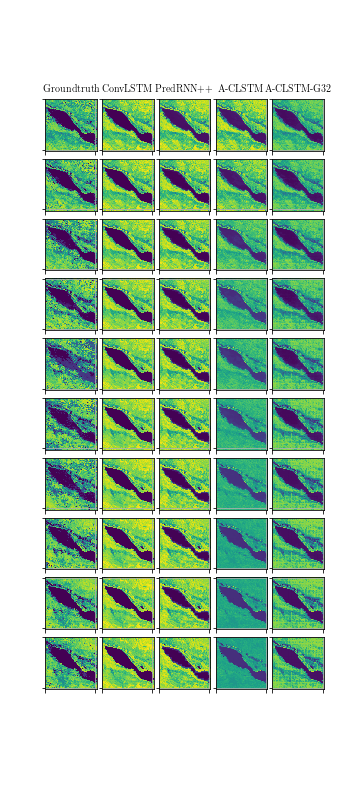
\includegraphics[width=.7\linewidth]{figures/chap4/10/30/groundtruth-predict-imgs.png}
    \caption{Example of 10 timesteps prediction at 21-28 August, 2016.}
    \label{fig:chap4-test-30-1}
\end{SCfigure}

\begin{figure}
    \begin{center}
        \begin{tabular}[b]{c}
            %% Creator: Matplotlib, PGF backend
%%
%% To include the figure in your LaTeX document, write
%%   \input{<filename>.pgf}
%%
%% Make sure the required packages are loaded in your preamble
%%   \usepackage{pgf}
%%
%% Figures using additional raster images can only be included by \input if
%% they are in the same directory as the main LaTeX file. For loading figures
%% from other directories you can use the `import` package
%%   \usepackage{import}
%% and then include the figures with
%%   \import{<path to file>}{<filename>.pgf}
%%
%% Matplotlib used the following preamble
%%   \usepackage{fontspec}
%%   \setmainfont{DejaVuSerif.ttf}[Path=/usr/local/lib/python3.6/dist-packages/matplotlib/mpl-data/fonts/ttf/]
%%   \setsansfont{DejaVuSans.ttf}[Path=/usr/local/lib/python3.6/dist-packages/matplotlib/mpl-data/fonts/ttf/]
%%   \setmonofont{DejaVuSansMono.ttf}[Path=/usr/local/lib/python3.6/dist-packages/matplotlib/mpl-data/fonts/ttf/]
%%
\begingroup%
\makeatletter%
\begin{pgfpicture}%
\pgfpathrectangle{\pgfpointorigin}{\pgfqpoint{5.000000in}{3.090170in}}%
\pgfusepath{use as bounding box, clip}%
\begin{pgfscope}%
\pgfsetbuttcap%
\pgfsetmiterjoin%
\definecolor{currentfill}{rgb}{1.000000,1.000000,1.000000}%
\pgfsetfillcolor{currentfill}%
\pgfsetlinewidth{0.000000pt}%
\definecolor{currentstroke}{rgb}{1.000000,1.000000,1.000000}%
\pgfsetstrokecolor{currentstroke}%
\pgfsetdash{}{0pt}%
\pgfpathmoveto{\pgfqpoint{0.000000in}{0.000000in}}%
\pgfpathlineto{\pgfqpoint{5.000000in}{0.000000in}}%
\pgfpathlineto{\pgfqpoint{5.000000in}{3.090170in}}%
\pgfpathlineto{\pgfqpoint{0.000000in}{3.090170in}}%
\pgfpathclose%
\pgfusepath{fill}%
\end{pgfscope}%
\begin{pgfscope}%
\pgfsetbuttcap%
\pgfsetmiterjoin%
\definecolor{currentfill}{rgb}{1.000000,1.000000,1.000000}%
\pgfsetfillcolor{currentfill}%
\pgfsetlinewidth{0.000000pt}%
\definecolor{currentstroke}{rgb}{0.000000,0.000000,0.000000}%
\pgfsetstrokecolor{currentstroke}%
\pgfsetstrokeopacity{0.000000}%
\pgfsetdash{}{0pt}%
\pgfpathmoveto{\pgfqpoint{0.625000in}{0.386271in}}%
\pgfpathlineto{\pgfqpoint{4.500000in}{0.386271in}}%
\pgfpathlineto{\pgfqpoint{4.500000in}{2.719350in}}%
\pgfpathlineto{\pgfqpoint{0.625000in}{2.719350in}}%
\pgfpathclose%
\pgfusepath{fill}%
\end{pgfscope}%
\begin{pgfscope}%
\pgfpathrectangle{\pgfqpoint{0.625000in}{0.386271in}}{\pgfqpoint{3.875000in}{2.333078in}}%
\pgfusepath{clip}%
\pgfsetrectcap%
\pgfsetroundjoin%
\pgfsetlinewidth{0.803000pt}%
\definecolor{currentstroke}{rgb}{0.690196,0.690196,0.690196}%
\pgfsetstrokecolor{currentstroke}%
\pgfsetdash{}{0pt}%
\pgfpathmoveto{\pgfqpoint{0.801136in}{0.386271in}}%
\pgfpathlineto{\pgfqpoint{0.801136in}{2.719350in}}%
\pgfusepath{stroke}%
\end{pgfscope}%
\begin{pgfscope}%
\pgfsetbuttcap%
\pgfsetroundjoin%
\definecolor{currentfill}{rgb}{0.501961,0.501961,0.501961}%
\pgfsetfillcolor{currentfill}%
\pgfsetlinewidth{0.803000pt}%
\definecolor{currentstroke}{rgb}{0.501961,0.501961,0.501961}%
\pgfsetstrokecolor{currentstroke}%
\pgfsetdash{}{0pt}%
\pgfsys@defobject{currentmarker}{\pgfqpoint{0.000000in}{-0.048611in}}{\pgfqpoint{0.000000in}{0.000000in}}{%
\pgfpathmoveto{\pgfqpoint{0.000000in}{0.000000in}}%
\pgfpathlineto{\pgfqpoint{0.000000in}{-0.048611in}}%
\pgfusepath{stroke,fill}%
}%
\begin{pgfscope}%
\pgfsys@transformshift{0.801136in}{0.386271in}%
\pgfsys@useobject{currentmarker}{}%
\end{pgfscope}%
\end{pgfscope}%
\begin{pgfscope}%
\definecolor{textcolor}{rgb}{0.000000,0.000000,0.000000}%
\pgfsetstrokecolor{textcolor}%
\pgfsetfillcolor{textcolor}%
\pgftext[x=0.801136in,y=0.289049in,,top]{\color{textcolor}\rmfamily\fontsize{10.000000}{12.000000}\selectfont 1}%
\end{pgfscope}%
\begin{pgfscope}%
\pgfpathrectangle{\pgfqpoint{0.625000in}{0.386271in}}{\pgfqpoint{3.875000in}{2.333078in}}%
\pgfusepath{clip}%
\pgfsetrectcap%
\pgfsetroundjoin%
\pgfsetlinewidth{0.803000pt}%
\definecolor{currentstroke}{rgb}{0.690196,0.690196,0.690196}%
\pgfsetstrokecolor{currentstroke}%
\pgfsetdash{}{0pt}%
\pgfpathmoveto{\pgfqpoint{1.583965in}{0.386271in}}%
\pgfpathlineto{\pgfqpoint{1.583965in}{2.719350in}}%
\pgfusepath{stroke}%
\end{pgfscope}%
\begin{pgfscope}%
\pgfsetbuttcap%
\pgfsetroundjoin%
\definecolor{currentfill}{rgb}{0.501961,0.501961,0.501961}%
\pgfsetfillcolor{currentfill}%
\pgfsetlinewidth{0.803000pt}%
\definecolor{currentstroke}{rgb}{0.501961,0.501961,0.501961}%
\pgfsetstrokecolor{currentstroke}%
\pgfsetdash{}{0pt}%
\pgfsys@defobject{currentmarker}{\pgfqpoint{0.000000in}{-0.048611in}}{\pgfqpoint{0.000000in}{0.000000in}}{%
\pgfpathmoveto{\pgfqpoint{0.000000in}{0.000000in}}%
\pgfpathlineto{\pgfqpoint{0.000000in}{-0.048611in}}%
\pgfusepath{stroke,fill}%
}%
\begin{pgfscope}%
\pgfsys@transformshift{1.583965in}{0.386271in}%
\pgfsys@useobject{currentmarker}{}%
\end{pgfscope}%
\end{pgfscope}%
\begin{pgfscope}%
\definecolor{textcolor}{rgb}{0.000000,0.000000,0.000000}%
\pgfsetstrokecolor{textcolor}%
\pgfsetfillcolor{textcolor}%
\pgftext[x=1.583965in,y=0.289049in,,top]{\color{textcolor}\rmfamily\fontsize{10.000000}{12.000000}\selectfont 2}%
\end{pgfscope}%
\begin{pgfscope}%
\pgfpathrectangle{\pgfqpoint{0.625000in}{0.386271in}}{\pgfqpoint{3.875000in}{2.333078in}}%
\pgfusepath{clip}%
\pgfsetrectcap%
\pgfsetroundjoin%
\pgfsetlinewidth{0.803000pt}%
\definecolor{currentstroke}{rgb}{0.690196,0.690196,0.690196}%
\pgfsetstrokecolor{currentstroke}%
\pgfsetdash{}{0pt}%
\pgfpathmoveto{\pgfqpoint{2.366793in}{0.386271in}}%
\pgfpathlineto{\pgfqpoint{2.366793in}{2.719350in}}%
\pgfusepath{stroke}%
\end{pgfscope}%
\begin{pgfscope}%
\pgfsetbuttcap%
\pgfsetroundjoin%
\definecolor{currentfill}{rgb}{0.501961,0.501961,0.501961}%
\pgfsetfillcolor{currentfill}%
\pgfsetlinewidth{0.803000pt}%
\definecolor{currentstroke}{rgb}{0.501961,0.501961,0.501961}%
\pgfsetstrokecolor{currentstroke}%
\pgfsetdash{}{0pt}%
\pgfsys@defobject{currentmarker}{\pgfqpoint{0.000000in}{-0.048611in}}{\pgfqpoint{0.000000in}{0.000000in}}{%
\pgfpathmoveto{\pgfqpoint{0.000000in}{0.000000in}}%
\pgfpathlineto{\pgfqpoint{0.000000in}{-0.048611in}}%
\pgfusepath{stroke,fill}%
}%
\begin{pgfscope}%
\pgfsys@transformshift{2.366793in}{0.386271in}%
\pgfsys@useobject{currentmarker}{}%
\end{pgfscope}%
\end{pgfscope}%
\begin{pgfscope}%
\definecolor{textcolor}{rgb}{0.000000,0.000000,0.000000}%
\pgfsetstrokecolor{textcolor}%
\pgfsetfillcolor{textcolor}%
\pgftext[x=2.366793in,y=0.289049in,,top]{\color{textcolor}\rmfamily\fontsize{10.000000}{12.000000}\selectfont 3}%
\end{pgfscope}%
\begin{pgfscope}%
\pgfpathrectangle{\pgfqpoint{0.625000in}{0.386271in}}{\pgfqpoint{3.875000in}{2.333078in}}%
\pgfusepath{clip}%
\pgfsetrectcap%
\pgfsetroundjoin%
\pgfsetlinewidth{0.803000pt}%
\definecolor{currentstroke}{rgb}{0.690196,0.690196,0.690196}%
\pgfsetstrokecolor{currentstroke}%
\pgfsetdash{}{0pt}%
\pgfpathmoveto{\pgfqpoint{3.149621in}{0.386271in}}%
\pgfpathlineto{\pgfqpoint{3.149621in}{2.719350in}}%
\pgfusepath{stroke}%
\end{pgfscope}%
\begin{pgfscope}%
\pgfsetbuttcap%
\pgfsetroundjoin%
\definecolor{currentfill}{rgb}{0.501961,0.501961,0.501961}%
\pgfsetfillcolor{currentfill}%
\pgfsetlinewidth{0.803000pt}%
\definecolor{currentstroke}{rgb}{0.501961,0.501961,0.501961}%
\pgfsetstrokecolor{currentstroke}%
\pgfsetdash{}{0pt}%
\pgfsys@defobject{currentmarker}{\pgfqpoint{0.000000in}{-0.048611in}}{\pgfqpoint{0.000000in}{0.000000in}}{%
\pgfpathmoveto{\pgfqpoint{0.000000in}{0.000000in}}%
\pgfpathlineto{\pgfqpoint{0.000000in}{-0.048611in}}%
\pgfusepath{stroke,fill}%
}%
\begin{pgfscope}%
\pgfsys@transformshift{3.149621in}{0.386271in}%
\pgfsys@useobject{currentmarker}{}%
\end{pgfscope}%
\end{pgfscope}%
\begin{pgfscope}%
\definecolor{textcolor}{rgb}{0.000000,0.000000,0.000000}%
\pgfsetstrokecolor{textcolor}%
\pgfsetfillcolor{textcolor}%
\pgftext[x=3.149621in,y=0.289049in,,top]{\color{textcolor}\rmfamily\fontsize{10.000000}{12.000000}\selectfont 4}%
\end{pgfscope}%
\begin{pgfscope}%
\pgfpathrectangle{\pgfqpoint{0.625000in}{0.386271in}}{\pgfqpoint{3.875000in}{2.333078in}}%
\pgfusepath{clip}%
\pgfsetrectcap%
\pgfsetroundjoin%
\pgfsetlinewidth{0.803000pt}%
\definecolor{currentstroke}{rgb}{0.690196,0.690196,0.690196}%
\pgfsetstrokecolor{currentstroke}%
\pgfsetdash{}{0pt}%
\pgfpathmoveto{\pgfqpoint{3.932449in}{0.386271in}}%
\pgfpathlineto{\pgfqpoint{3.932449in}{2.719350in}}%
\pgfusepath{stroke}%
\end{pgfscope}%
\begin{pgfscope}%
\pgfsetbuttcap%
\pgfsetroundjoin%
\definecolor{currentfill}{rgb}{0.501961,0.501961,0.501961}%
\pgfsetfillcolor{currentfill}%
\pgfsetlinewidth{0.803000pt}%
\definecolor{currentstroke}{rgb}{0.501961,0.501961,0.501961}%
\pgfsetstrokecolor{currentstroke}%
\pgfsetdash{}{0pt}%
\pgfsys@defobject{currentmarker}{\pgfqpoint{0.000000in}{-0.048611in}}{\pgfqpoint{0.000000in}{0.000000in}}{%
\pgfpathmoveto{\pgfqpoint{0.000000in}{0.000000in}}%
\pgfpathlineto{\pgfqpoint{0.000000in}{-0.048611in}}%
\pgfusepath{stroke,fill}%
}%
\begin{pgfscope}%
\pgfsys@transformshift{3.932449in}{0.386271in}%
\pgfsys@useobject{currentmarker}{}%
\end{pgfscope}%
\end{pgfscope}%
\begin{pgfscope}%
\definecolor{textcolor}{rgb}{0.000000,0.000000,0.000000}%
\pgfsetstrokecolor{textcolor}%
\pgfsetfillcolor{textcolor}%
\pgftext[x=3.932449in,y=0.289049in,,top]{\color{textcolor}\rmfamily\fontsize{10.000000}{12.000000}\selectfont 5}%
\end{pgfscope}%
\begin{pgfscope}%
\definecolor{textcolor}{rgb}{0.000000,0.000000,0.000000}%
\pgfsetstrokecolor{textcolor}%
\pgfsetfillcolor{textcolor}%
\pgftext[x=2.562500in,y=0.099081in,,top]{\color{textcolor}\rmfamily\fontsize{10.000000}{12.000000}\selectfont Steps Prediction}%
\end{pgfscope}%
\begin{pgfscope}%
\pgfpathrectangle{\pgfqpoint{0.625000in}{0.386271in}}{\pgfqpoint{3.875000in}{2.333078in}}%
\pgfusepath{clip}%
\pgfsetrectcap%
\pgfsetroundjoin%
\pgfsetlinewidth{0.803000pt}%
\definecolor{currentstroke}{rgb}{0.690196,0.690196,0.690196}%
\pgfsetstrokecolor{currentstroke}%
\pgfsetdash{}{0pt}%
\pgfpathmoveto{\pgfqpoint{0.625000in}{0.565076in}}%
\pgfpathlineto{\pgfqpoint{4.500000in}{0.565076in}}%
\pgfusepath{stroke}%
\end{pgfscope}%
\begin{pgfscope}%
\pgfsetbuttcap%
\pgfsetroundjoin%
\definecolor{currentfill}{rgb}{0.501961,0.501961,0.501961}%
\pgfsetfillcolor{currentfill}%
\pgfsetlinewidth{0.803000pt}%
\definecolor{currentstroke}{rgb}{0.501961,0.501961,0.501961}%
\pgfsetstrokecolor{currentstroke}%
\pgfsetdash{}{0pt}%
\pgfsys@defobject{currentmarker}{\pgfqpoint{-0.048611in}{0.000000in}}{\pgfqpoint{0.000000in}{0.000000in}}{%
\pgfpathmoveto{\pgfqpoint{0.000000in}{0.000000in}}%
\pgfpathlineto{\pgfqpoint{-0.048611in}{0.000000in}}%
\pgfusepath{stroke,fill}%
}%
\begin{pgfscope}%
\pgfsys@transformshift{0.625000in}{0.565076in}%
\pgfsys@useobject{currentmarker}{}%
\end{pgfscope}%
\end{pgfscope}%
\begin{pgfscope}%
\definecolor{textcolor}{rgb}{0.000000,0.000000,0.000000}%
\pgfsetstrokecolor{textcolor}%
\pgfsetfillcolor{textcolor}%
\pgftext[x=0.280863in,y=0.512315in,left,base]{\color{textcolor}\rmfamily\fontsize{10.000000}{12.000000}\selectfont \(\displaystyle 0.02\)}%
\end{pgfscope}%
\begin{pgfscope}%
\pgfpathrectangle{\pgfqpoint{0.625000in}{0.386271in}}{\pgfqpoint{3.875000in}{2.333078in}}%
\pgfusepath{clip}%
\pgfsetrectcap%
\pgfsetroundjoin%
\pgfsetlinewidth{0.803000pt}%
\definecolor{currentstroke}{rgb}{0.690196,0.690196,0.690196}%
\pgfsetstrokecolor{currentstroke}%
\pgfsetdash{}{0pt}%
\pgfpathmoveto{\pgfqpoint{0.625000in}{0.889426in}}%
\pgfpathlineto{\pgfqpoint{4.500000in}{0.889426in}}%
\pgfusepath{stroke}%
\end{pgfscope}%
\begin{pgfscope}%
\pgfsetbuttcap%
\pgfsetroundjoin%
\definecolor{currentfill}{rgb}{0.501961,0.501961,0.501961}%
\pgfsetfillcolor{currentfill}%
\pgfsetlinewidth{0.803000pt}%
\definecolor{currentstroke}{rgb}{0.501961,0.501961,0.501961}%
\pgfsetstrokecolor{currentstroke}%
\pgfsetdash{}{0pt}%
\pgfsys@defobject{currentmarker}{\pgfqpoint{-0.048611in}{0.000000in}}{\pgfqpoint{0.000000in}{0.000000in}}{%
\pgfpathmoveto{\pgfqpoint{0.000000in}{0.000000in}}%
\pgfpathlineto{\pgfqpoint{-0.048611in}{0.000000in}}%
\pgfusepath{stroke,fill}%
}%
\begin{pgfscope}%
\pgfsys@transformshift{0.625000in}{0.889426in}%
\pgfsys@useobject{currentmarker}{}%
\end{pgfscope}%
\end{pgfscope}%
\begin{pgfscope}%
\definecolor{textcolor}{rgb}{0.000000,0.000000,0.000000}%
\pgfsetstrokecolor{textcolor}%
\pgfsetfillcolor{textcolor}%
\pgftext[x=0.280863in,y=0.836664in,left,base]{\color{textcolor}\rmfamily\fontsize{10.000000}{12.000000}\selectfont \(\displaystyle 0.04\)}%
\end{pgfscope}%
\begin{pgfscope}%
\pgfpathrectangle{\pgfqpoint{0.625000in}{0.386271in}}{\pgfqpoint{3.875000in}{2.333078in}}%
\pgfusepath{clip}%
\pgfsetrectcap%
\pgfsetroundjoin%
\pgfsetlinewidth{0.803000pt}%
\definecolor{currentstroke}{rgb}{0.690196,0.690196,0.690196}%
\pgfsetstrokecolor{currentstroke}%
\pgfsetdash{}{0pt}%
\pgfpathmoveto{\pgfqpoint{0.625000in}{1.213775in}}%
\pgfpathlineto{\pgfqpoint{4.500000in}{1.213775in}}%
\pgfusepath{stroke}%
\end{pgfscope}%
\begin{pgfscope}%
\pgfsetbuttcap%
\pgfsetroundjoin%
\definecolor{currentfill}{rgb}{0.501961,0.501961,0.501961}%
\pgfsetfillcolor{currentfill}%
\pgfsetlinewidth{0.803000pt}%
\definecolor{currentstroke}{rgb}{0.501961,0.501961,0.501961}%
\pgfsetstrokecolor{currentstroke}%
\pgfsetdash{}{0pt}%
\pgfsys@defobject{currentmarker}{\pgfqpoint{-0.048611in}{0.000000in}}{\pgfqpoint{0.000000in}{0.000000in}}{%
\pgfpathmoveto{\pgfqpoint{0.000000in}{0.000000in}}%
\pgfpathlineto{\pgfqpoint{-0.048611in}{0.000000in}}%
\pgfusepath{stroke,fill}%
}%
\begin{pgfscope}%
\pgfsys@transformshift{0.625000in}{1.213775in}%
\pgfsys@useobject{currentmarker}{}%
\end{pgfscope}%
\end{pgfscope}%
\begin{pgfscope}%
\definecolor{textcolor}{rgb}{0.000000,0.000000,0.000000}%
\pgfsetstrokecolor{textcolor}%
\pgfsetfillcolor{textcolor}%
\pgftext[x=0.280863in,y=1.161013in,left,base]{\color{textcolor}\rmfamily\fontsize{10.000000}{12.000000}\selectfont \(\displaystyle 0.06\)}%
\end{pgfscope}%
\begin{pgfscope}%
\pgfpathrectangle{\pgfqpoint{0.625000in}{0.386271in}}{\pgfqpoint{3.875000in}{2.333078in}}%
\pgfusepath{clip}%
\pgfsetrectcap%
\pgfsetroundjoin%
\pgfsetlinewidth{0.803000pt}%
\definecolor{currentstroke}{rgb}{0.690196,0.690196,0.690196}%
\pgfsetstrokecolor{currentstroke}%
\pgfsetdash{}{0pt}%
\pgfpathmoveto{\pgfqpoint{0.625000in}{1.538124in}}%
\pgfpathlineto{\pgfqpoint{4.500000in}{1.538124in}}%
\pgfusepath{stroke}%
\end{pgfscope}%
\begin{pgfscope}%
\pgfsetbuttcap%
\pgfsetroundjoin%
\definecolor{currentfill}{rgb}{0.501961,0.501961,0.501961}%
\pgfsetfillcolor{currentfill}%
\pgfsetlinewidth{0.803000pt}%
\definecolor{currentstroke}{rgb}{0.501961,0.501961,0.501961}%
\pgfsetstrokecolor{currentstroke}%
\pgfsetdash{}{0pt}%
\pgfsys@defobject{currentmarker}{\pgfqpoint{-0.048611in}{0.000000in}}{\pgfqpoint{0.000000in}{0.000000in}}{%
\pgfpathmoveto{\pgfqpoint{0.000000in}{0.000000in}}%
\pgfpathlineto{\pgfqpoint{-0.048611in}{0.000000in}}%
\pgfusepath{stroke,fill}%
}%
\begin{pgfscope}%
\pgfsys@transformshift{0.625000in}{1.538124in}%
\pgfsys@useobject{currentmarker}{}%
\end{pgfscope}%
\end{pgfscope}%
\begin{pgfscope}%
\definecolor{textcolor}{rgb}{0.000000,0.000000,0.000000}%
\pgfsetstrokecolor{textcolor}%
\pgfsetfillcolor{textcolor}%
\pgftext[x=0.280863in,y=1.485363in,left,base]{\color{textcolor}\rmfamily\fontsize{10.000000}{12.000000}\selectfont \(\displaystyle 0.08\)}%
\end{pgfscope}%
\begin{pgfscope}%
\pgfpathrectangle{\pgfqpoint{0.625000in}{0.386271in}}{\pgfqpoint{3.875000in}{2.333078in}}%
\pgfusepath{clip}%
\pgfsetrectcap%
\pgfsetroundjoin%
\pgfsetlinewidth{0.803000pt}%
\definecolor{currentstroke}{rgb}{0.690196,0.690196,0.690196}%
\pgfsetstrokecolor{currentstroke}%
\pgfsetdash{}{0pt}%
\pgfpathmoveto{\pgfqpoint{0.625000in}{1.862473in}}%
\pgfpathlineto{\pgfqpoint{4.500000in}{1.862473in}}%
\pgfusepath{stroke}%
\end{pgfscope}%
\begin{pgfscope}%
\pgfsetbuttcap%
\pgfsetroundjoin%
\definecolor{currentfill}{rgb}{0.501961,0.501961,0.501961}%
\pgfsetfillcolor{currentfill}%
\pgfsetlinewidth{0.803000pt}%
\definecolor{currentstroke}{rgb}{0.501961,0.501961,0.501961}%
\pgfsetstrokecolor{currentstroke}%
\pgfsetdash{}{0pt}%
\pgfsys@defobject{currentmarker}{\pgfqpoint{-0.048611in}{0.000000in}}{\pgfqpoint{0.000000in}{0.000000in}}{%
\pgfpathmoveto{\pgfqpoint{0.000000in}{0.000000in}}%
\pgfpathlineto{\pgfqpoint{-0.048611in}{0.000000in}}%
\pgfusepath{stroke,fill}%
}%
\begin{pgfscope}%
\pgfsys@transformshift{0.625000in}{1.862473in}%
\pgfsys@useobject{currentmarker}{}%
\end{pgfscope}%
\end{pgfscope}%
\begin{pgfscope}%
\definecolor{textcolor}{rgb}{0.000000,0.000000,0.000000}%
\pgfsetstrokecolor{textcolor}%
\pgfsetfillcolor{textcolor}%
\pgftext[x=0.280863in,y=1.809712in,left,base]{\color{textcolor}\rmfamily\fontsize{10.000000}{12.000000}\selectfont \(\displaystyle 0.10\)}%
\end{pgfscope}%
\begin{pgfscope}%
\pgfpathrectangle{\pgfqpoint{0.625000in}{0.386271in}}{\pgfqpoint{3.875000in}{2.333078in}}%
\pgfusepath{clip}%
\pgfsetrectcap%
\pgfsetroundjoin%
\pgfsetlinewidth{0.803000pt}%
\definecolor{currentstroke}{rgb}{0.690196,0.690196,0.690196}%
\pgfsetstrokecolor{currentstroke}%
\pgfsetdash{}{0pt}%
\pgfpathmoveto{\pgfqpoint{0.625000in}{2.186823in}}%
\pgfpathlineto{\pgfqpoint{4.500000in}{2.186823in}}%
\pgfusepath{stroke}%
\end{pgfscope}%
\begin{pgfscope}%
\pgfsetbuttcap%
\pgfsetroundjoin%
\definecolor{currentfill}{rgb}{0.501961,0.501961,0.501961}%
\pgfsetfillcolor{currentfill}%
\pgfsetlinewidth{0.803000pt}%
\definecolor{currentstroke}{rgb}{0.501961,0.501961,0.501961}%
\pgfsetstrokecolor{currentstroke}%
\pgfsetdash{}{0pt}%
\pgfsys@defobject{currentmarker}{\pgfqpoint{-0.048611in}{0.000000in}}{\pgfqpoint{0.000000in}{0.000000in}}{%
\pgfpathmoveto{\pgfqpoint{0.000000in}{0.000000in}}%
\pgfpathlineto{\pgfqpoint{-0.048611in}{0.000000in}}%
\pgfusepath{stroke,fill}%
}%
\begin{pgfscope}%
\pgfsys@transformshift{0.625000in}{2.186823in}%
\pgfsys@useobject{currentmarker}{}%
\end{pgfscope}%
\end{pgfscope}%
\begin{pgfscope}%
\definecolor{textcolor}{rgb}{0.000000,0.000000,0.000000}%
\pgfsetstrokecolor{textcolor}%
\pgfsetfillcolor{textcolor}%
\pgftext[x=0.280863in,y=2.134061in,left,base]{\color{textcolor}\rmfamily\fontsize{10.000000}{12.000000}\selectfont \(\displaystyle 0.12\)}%
\end{pgfscope}%
\begin{pgfscope}%
\pgfpathrectangle{\pgfqpoint{0.625000in}{0.386271in}}{\pgfqpoint{3.875000in}{2.333078in}}%
\pgfusepath{clip}%
\pgfsetrectcap%
\pgfsetroundjoin%
\pgfsetlinewidth{0.803000pt}%
\definecolor{currentstroke}{rgb}{0.690196,0.690196,0.690196}%
\pgfsetstrokecolor{currentstroke}%
\pgfsetdash{}{0pt}%
\pgfpathmoveto{\pgfqpoint{0.625000in}{2.511172in}}%
\pgfpathlineto{\pgfqpoint{4.500000in}{2.511172in}}%
\pgfusepath{stroke}%
\end{pgfscope}%
\begin{pgfscope}%
\pgfsetbuttcap%
\pgfsetroundjoin%
\definecolor{currentfill}{rgb}{0.501961,0.501961,0.501961}%
\pgfsetfillcolor{currentfill}%
\pgfsetlinewidth{0.803000pt}%
\definecolor{currentstroke}{rgb}{0.501961,0.501961,0.501961}%
\pgfsetstrokecolor{currentstroke}%
\pgfsetdash{}{0pt}%
\pgfsys@defobject{currentmarker}{\pgfqpoint{-0.048611in}{0.000000in}}{\pgfqpoint{0.000000in}{0.000000in}}{%
\pgfpathmoveto{\pgfqpoint{0.000000in}{0.000000in}}%
\pgfpathlineto{\pgfqpoint{-0.048611in}{0.000000in}}%
\pgfusepath{stroke,fill}%
}%
\begin{pgfscope}%
\pgfsys@transformshift{0.625000in}{2.511172in}%
\pgfsys@useobject{currentmarker}{}%
\end{pgfscope}%
\end{pgfscope}%
\begin{pgfscope}%
\definecolor{textcolor}{rgb}{0.000000,0.000000,0.000000}%
\pgfsetstrokecolor{textcolor}%
\pgfsetfillcolor{textcolor}%
\pgftext[x=0.280863in,y=2.458411in,left,base]{\color{textcolor}\rmfamily\fontsize{10.000000}{12.000000}\selectfont \(\displaystyle 0.14\)}%
\end{pgfscope}%
\begin{pgfscope}%
\definecolor{textcolor}{rgb}{0.000000,0.000000,0.000000}%
\pgfsetstrokecolor{textcolor}%
\pgfsetfillcolor{textcolor}%
\pgftext[x=0.225308in,y=1.552810in,,bottom,rotate=90.000000]{\color{textcolor}\rmfamily\fontsize{10.000000}{12.000000}\selectfont Water-NRMSE}%
\end{pgfscope}%
\begin{pgfscope}%
\pgfpathrectangle{\pgfqpoint{0.625000in}{0.386271in}}{\pgfqpoint{3.875000in}{2.333078in}}%
\pgfusepath{clip}%
\pgfsetrectcap%
\pgfsetroundjoin%
\pgfsetlinewidth{1.505625pt}%
\definecolor{currentstroke}{rgb}{1.000000,0.000000,0.000000}%
\pgfsetstrokecolor{currentstroke}%
\pgfsetdash{}{0pt}%
\pgfpathmoveto{\pgfqpoint{0.801136in}{0.638545in}}%
\pgfpathlineto{\pgfqpoint{1.192551in}{1.081163in}}%
\pgfpathlineto{\pgfqpoint{1.583965in}{1.363219in}}%
\pgfpathlineto{\pgfqpoint{1.975379in}{1.593309in}}%
\pgfpathlineto{\pgfqpoint{2.366793in}{1.936651in}}%
\pgfpathlineto{\pgfqpoint{2.758207in}{1.529515in}}%
\pgfpathlineto{\pgfqpoint{3.149621in}{1.591517in}}%
\pgfpathlineto{\pgfqpoint{3.541035in}{1.421996in}}%
\pgfpathlineto{\pgfqpoint{3.932449in}{1.176854in}}%
\pgfpathlineto{\pgfqpoint{4.323864in}{1.827341in}}%
\pgfusepath{stroke}%
\end{pgfscope}%
\begin{pgfscope}%
\pgfpathrectangle{\pgfqpoint{0.625000in}{0.386271in}}{\pgfqpoint{3.875000in}{2.333078in}}%
\pgfusepath{clip}%
\pgfsetbuttcap%
\pgfsetroundjoin%
\definecolor{currentfill}{rgb}{1.000000,0.000000,0.000000}%
\pgfsetfillcolor{currentfill}%
\pgfsetlinewidth{1.003750pt}%
\definecolor{currentstroke}{rgb}{1.000000,0.000000,0.000000}%
\pgfsetstrokecolor{currentstroke}%
\pgfsetdash{}{0pt}%
\pgfsys@defobject{currentmarker}{\pgfqpoint{-0.041667in}{-0.041667in}}{\pgfqpoint{0.041667in}{0.041667in}}{%
\pgfpathmoveto{\pgfqpoint{0.000000in}{-0.041667in}}%
\pgfpathcurveto{\pgfqpoint{0.011050in}{-0.041667in}}{\pgfqpoint{0.021649in}{-0.037276in}}{\pgfqpoint{0.029463in}{-0.029463in}}%
\pgfpathcurveto{\pgfqpoint{0.037276in}{-0.021649in}}{\pgfqpoint{0.041667in}{-0.011050in}}{\pgfqpoint{0.041667in}{0.000000in}}%
\pgfpathcurveto{\pgfqpoint{0.041667in}{0.011050in}}{\pgfqpoint{0.037276in}{0.021649in}}{\pgfqpoint{0.029463in}{0.029463in}}%
\pgfpathcurveto{\pgfqpoint{0.021649in}{0.037276in}}{\pgfqpoint{0.011050in}{0.041667in}}{\pgfqpoint{0.000000in}{0.041667in}}%
\pgfpathcurveto{\pgfqpoint{-0.011050in}{0.041667in}}{\pgfqpoint{-0.021649in}{0.037276in}}{\pgfqpoint{-0.029463in}{0.029463in}}%
\pgfpathcurveto{\pgfqpoint{-0.037276in}{0.021649in}}{\pgfqpoint{-0.041667in}{0.011050in}}{\pgfqpoint{-0.041667in}{0.000000in}}%
\pgfpathcurveto{\pgfqpoint{-0.041667in}{-0.011050in}}{\pgfqpoint{-0.037276in}{-0.021649in}}{\pgfqpoint{-0.029463in}{-0.029463in}}%
\pgfpathcurveto{\pgfqpoint{-0.021649in}{-0.037276in}}{\pgfqpoint{-0.011050in}{-0.041667in}}{\pgfqpoint{0.000000in}{-0.041667in}}%
\pgfpathclose%
\pgfusepath{stroke,fill}%
}%
\begin{pgfscope}%
\pgfsys@transformshift{0.801136in}{0.638545in}%
\pgfsys@useobject{currentmarker}{}%
\end{pgfscope}%
\begin{pgfscope}%
\pgfsys@transformshift{1.192551in}{1.081163in}%
\pgfsys@useobject{currentmarker}{}%
\end{pgfscope}%
\begin{pgfscope}%
\pgfsys@transformshift{1.583965in}{1.363219in}%
\pgfsys@useobject{currentmarker}{}%
\end{pgfscope}%
\begin{pgfscope}%
\pgfsys@transformshift{1.975379in}{1.593309in}%
\pgfsys@useobject{currentmarker}{}%
\end{pgfscope}%
\begin{pgfscope}%
\pgfsys@transformshift{2.366793in}{1.936651in}%
\pgfsys@useobject{currentmarker}{}%
\end{pgfscope}%
\begin{pgfscope}%
\pgfsys@transformshift{2.758207in}{1.529515in}%
\pgfsys@useobject{currentmarker}{}%
\end{pgfscope}%
\begin{pgfscope}%
\pgfsys@transformshift{3.149621in}{1.591517in}%
\pgfsys@useobject{currentmarker}{}%
\end{pgfscope}%
\begin{pgfscope}%
\pgfsys@transformshift{3.541035in}{1.421996in}%
\pgfsys@useobject{currentmarker}{}%
\end{pgfscope}%
\begin{pgfscope}%
\pgfsys@transformshift{3.932449in}{1.176854in}%
\pgfsys@useobject{currentmarker}{}%
\end{pgfscope}%
\begin{pgfscope}%
\pgfsys@transformshift{4.323864in}{1.827341in}%
\pgfsys@useobject{currentmarker}{}%
\end{pgfscope}%
\end{pgfscope}%
\begin{pgfscope}%
\pgfpathrectangle{\pgfqpoint{0.625000in}{0.386271in}}{\pgfqpoint{3.875000in}{2.333078in}}%
\pgfusepath{clip}%
\pgfsetrectcap%
\pgfsetroundjoin%
\pgfsetlinewidth{1.505625pt}%
\definecolor{currentstroke}{rgb}{0.000000,0.500000,0.000000}%
\pgfsetstrokecolor{currentstroke}%
\pgfsetdash{}{0pt}%
\pgfpathmoveto{\pgfqpoint{0.801136in}{0.605931in}}%
\pgfpathlineto{\pgfqpoint{1.192551in}{1.157501in}}%
\pgfpathlineto{\pgfqpoint{1.583965in}{1.566788in}}%
\pgfpathlineto{\pgfqpoint{1.975379in}{1.965681in}}%
\pgfpathlineto{\pgfqpoint{2.366793in}{2.431236in}}%
\pgfpathlineto{\pgfqpoint{2.758207in}{2.090044in}}%
\pgfpathlineto{\pgfqpoint{3.149621in}{2.214049in}}%
\pgfpathlineto{\pgfqpoint{3.541035in}{2.107964in}}%
\pgfpathlineto{\pgfqpoint{3.932449in}{1.936293in}}%
\pgfpathlineto{\pgfqpoint{4.323864in}{2.613301in}}%
\pgfusepath{stroke}%
\end{pgfscope}%
\begin{pgfscope}%
\pgfpathrectangle{\pgfqpoint{0.625000in}{0.386271in}}{\pgfqpoint{3.875000in}{2.333078in}}%
\pgfusepath{clip}%
\pgfsetbuttcap%
\pgfsetroundjoin%
\definecolor{currentfill}{rgb}{0.000000,0.500000,0.000000}%
\pgfsetfillcolor{currentfill}%
\pgfsetlinewidth{1.003750pt}%
\definecolor{currentstroke}{rgb}{0.000000,0.500000,0.000000}%
\pgfsetstrokecolor{currentstroke}%
\pgfsetdash{}{0pt}%
\pgfsys@defobject{currentmarker}{\pgfqpoint{-0.041667in}{-0.041667in}}{\pgfqpoint{0.041667in}{0.041667in}}{%
\pgfpathmoveto{\pgfqpoint{-0.041667in}{-0.041667in}}%
\pgfpathlineto{\pgfqpoint{0.041667in}{0.041667in}}%
\pgfpathmoveto{\pgfqpoint{-0.041667in}{0.041667in}}%
\pgfpathlineto{\pgfqpoint{0.041667in}{-0.041667in}}%
\pgfusepath{stroke,fill}%
}%
\begin{pgfscope}%
\pgfsys@transformshift{0.801136in}{0.605931in}%
\pgfsys@useobject{currentmarker}{}%
\end{pgfscope}%
\begin{pgfscope}%
\pgfsys@transformshift{1.192551in}{1.157501in}%
\pgfsys@useobject{currentmarker}{}%
\end{pgfscope}%
\begin{pgfscope}%
\pgfsys@transformshift{1.583965in}{1.566788in}%
\pgfsys@useobject{currentmarker}{}%
\end{pgfscope}%
\begin{pgfscope}%
\pgfsys@transformshift{1.975379in}{1.965681in}%
\pgfsys@useobject{currentmarker}{}%
\end{pgfscope}%
\begin{pgfscope}%
\pgfsys@transformshift{2.366793in}{2.431236in}%
\pgfsys@useobject{currentmarker}{}%
\end{pgfscope}%
\begin{pgfscope}%
\pgfsys@transformshift{2.758207in}{2.090044in}%
\pgfsys@useobject{currentmarker}{}%
\end{pgfscope}%
\begin{pgfscope}%
\pgfsys@transformshift{3.149621in}{2.214049in}%
\pgfsys@useobject{currentmarker}{}%
\end{pgfscope}%
\begin{pgfscope}%
\pgfsys@transformshift{3.541035in}{2.107964in}%
\pgfsys@useobject{currentmarker}{}%
\end{pgfscope}%
\begin{pgfscope}%
\pgfsys@transformshift{3.932449in}{1.936293in}%
\pgfsys@useobject{currentmarker}{}%
\end{pgfscope}%
\begin{pgfscope}%
\pgfsys@transformshift{4.323864in}{2.613301in}%
\pgfsys@useobject{currentmarker}{}%
\end{pgfscope}%
\end{pgfscope}%
\begin{pgfscope}%
\pgfpathrectangle{\pgfqpoint{0.625000in}{0.386271in}}{\pgfqpoint{3.875000in}{2.333078in}}%
\pgfusepath{clip}%
\pgfsetrectcap%
\pgfsetroundjoin%
\pgfsetlinewidth{1.505625pt}%
\definecolor{currentstroke}{rgb}{0.000000,0.000000,1.000000}%
\pgfsetstrokecolor{currentstroke}%
\pgfsetdash{}{0pt}%
\pgfpathmoveto{\pgfqpoint{0.801136in}{0.600555in}}%
\pgfpathlineto{\pgfqpoint{1.192551in}{0.809500in}}%
\pgfpathlineto{\pgfqpoint{1.583965in}{0.986905in}}%
\pgfpathlineto{\pgfqpoint{1.975379in}{1.170762in}}%
\pgfpathlineto{\pgfqpoint{2.366793in}{1.411244in}}%
\pgfpathlineto{\pgfqpoint{2.758207in}{0.892647in}}%
\pgfpathlineto{\pgfqpoint{3.149621in}{0.987622in}}%
\pgfpathlineto{\pgfqpoint{3.541035in}{0.818101in}}%
\pgfpathlineto{\pgfqpoint{3.932449in}{0.591596in}}%
\pgfpathlineto{\pgfqpoint{4.323864in}{1.300142in}}%
\pgfusepath{stroke}%
\end{pgfscope}%
\begin{pgfscope}%
\pgfpathrectangle{\pgfqpoint{0.625000in}{0.386271in}}{\pgfqpoint{3.875000in}{2.333078in}}%
\pgfusepath{clip}%
\pgfsetbuttcap%
\pgfsetmiterjoin%
\definecolor{currentfill}{rgb}{0.000000,0.000000,1.000000}%
\pgfsetfillcolor{currentfill}%
\pgfsetlinewidth{1.003750pt}%
\definecolor{currentstroke}{rgb}{0.000000,0.000000,1.000000}%
\pgfsetstrokecolor{currentstroke}%
\pgfsetdash{}{0pt}%
\pgfsys@defobject{currentmarker}{\pgfqpoint{-0.058926in}{-0.058926in}}{\pgfqpoint{0.058926in}{0.058926in}}{%
\pgfpathmoveto{\pgfqpoint{-0.000000in}{-0.058926in}}%
\pgfpathlineto{\pgfqpoint{0.058926in}{0.000000in}}%
\pgfpathlineto{\pgfqpoint{0.000000in}{0.058926in}}%
\pgfpathlineto{\pgfqpoint{-0.058926in}{0.000000in}}%
\pgfpathclose%
\pgfusepath{stroke,fill}%
}%
\begin{pgfscope}%
\pgfsys@transformshift{0.801136in}{0.600555in}%
\pgfsys@useobject{currentmarker}{}%
\end{pgfscope}%
\begin{pgfscope}%
\pgfsys@transformshift{1.192551in}{0.809500in}%
\pgfsys@useobject{currentmarker}{}%
\end{pgfscope}%
\begin{pgfscope}%
\pgfsys@transformshift{1.583965in}{0.986905in}%
\pgfsys@useobject{currentmarker}{}%
\end{pgfscope}%
\begin{pgfscope}%
\pgfsys@transformshift{1.975379in}{1.170762in}%
\pgfsys@useobject{currentmarker}{}%
\end{pgfscope}%
\begin{pgfscope}%
\pgfsys@transformshift{2.366793in}{1.411244in}%
\pgfsys@useobject{currentmarker}{}%
\end{pgfscope}%
\begin{pgfscope}%
\pgfsys@transformshift{2.758207in}{0.892647in}%
\pgfsys@useobject{currentmarker}{}%
\end{pgfscope}%
\begin{pgfscope}%
\pgfsys@transformshift{3.149621in}{0.987622in}%
\pgfsys@useobject{currentmarker}{}%
\end{pgfscope}%
\begin{pgfscope}%
\pgfsys@transformshift{3.541035in}{0.818101in}%
\pgfsys@useobject{currentmarker}{}%
\end{pgfscope}%
\begin{pgfscope}%
\pgfsys@transformshift{3.932449in}{0.591596in}%
\pgfsys@useobject{currentmarker}{}%
\end{pgfscope}%
\begin{pgfscope}%
\pgfsys@transformshift{4.323864in}{1.300142in}%
\pgfsys@useobject{currentmarker}{}%
\end{pgfscope}%
\end{pgfscope}%
\begin{pgfscope}%
\pgfpathrectangle{\pgfqpoint{0.625000in}{0.386271in}}{\pgfqpoint{3.875000in}{2.333078in}}%
\pgfusepath{clip}%
\pgfsetrectcap%
\pgfsetroundjoin%
\pgfsetlinewidth{1.505625pt}%
\definecolor{currentstroke}{rgb}{1.000000,1.000000,0.000000}%
\pgfsetstrokecolor{currentstroke}%
\pgfsetdash{}{0pt}%
\pgfpathmoveto{\pgfqpoint{0.801136in}{0.492320in}}%
\pgfpathlineto{\pgfqpoint{1.192551in}{0.690154in}}%
\pgfpathlineto{\pgfqpoint{1.583965in}{0.904474in}}%
\pgfpathlineto{\pgfqpoint{1.975379in}{1.065394in}}%
\pgfpathlineto{\pgfqpoint{2.366793in}{1.428806in}}%
\pgfpathlineto{\pgfqpoint{2.758207in}{0.996223in}}%
\pgfpathlineto{\pgfqpoint{3.149621in}{1.079013in}}%
\pgfpathlineto{\pgfqpoint{3.541035in}{0.938880in}}%
\pgfpathlineto{\pgfqpoint{3.932449in}{0.711299in}}%
\pgfpathlineto{\pgfqpoint{4.323864in}{1.380422in}}%
\pgfusepath{stroke}%
\end{pgfscope}%
\begin{pgfscope}%
\pgfpathrectangle{\pgfqpoint{0.625000in}{0.386271in}}{\pgfqpoint{3.875000in}{2.333078in}}%
\pgfusepath{clip}%
\pgfsetbuttcap%
\pgfsetbeveljoin%
\definecolor{currentfill}{rgb}{1.000000,1.000000,0.000000}%
\pgfsetfillcolor{currentfill}%
\pgfsetlinewidth{1.003750pt}%
\definecolor{currentstroke}{rgb}{1.000000,1.000000,0.000000}%
\pgfsetstrokecolor{currentstroke}%
\pgfsetdash{}{0pt}%
\pgfsys@defobject{currentmarker}{\pgfqpoint{-0.039627in}{-0.033709in}}{\pgfqpoint{0.039627in}{0.041667in}}{%
\pgfpathmoveto{\pgfqpoint{0.000000in}{0.041667in}}%
\pgfpathlineto{\pgfqpoint{-0.009355in}{0.012876in}}%
\pgfpathlineto{\pgfqpoint{-0.039627in}{0.012876in}}%
\pgfpathlineto{\pgfqpoint{-0.015136in}{-0.004918in}}%
\pgfpathlineto{\pgfqpoint{-0.024491in}{-0.033709in}}%
\pgfpathlineto{\pgfqpoint{-0.000000in}{-0.015915in}}%
\pgfpathlineto{\pgfqpoint{0.024491in}{-0.033709in}}%
\pgfpathlineto{\pgfqpoint{0.015136in}{-0.004918in}}%
\pgfpathlineto{\pgfqpoint{0.039627in}{0.012876in}}%
\pgfpathlineto{\pgfqpoint{0.009355in}{0.012876in}}%
\pgfpathclose%
\pgfusepath{stroke,fill}%
}%
\begin{pgfscope}%
\pgfsys@transformshift{0.801136in}{0.492320in}%
\pgfsys@useobject{currentmarker}{}%
\end{pgfscope}%
\begin{pgfscope}%
\pgfsys@transformshift{1.192551in}{0.690154in}%
\pgfsys@useobject{currentmarker}{}%
\end{pgfscope}%
\begin{pgfscope}%
\pgfsys@transformshift{1.583965in}{0.904474in}%
\pgfsys@useobject{currentmarker}{}%
\end{pgfscope}%
\begin{pgfscope}%
\pgfsys@transformshift{1.975379in}{1.065394in}%
\pgfsys@useobject{currentmarker}{}%
\end{pgfscope}%
\begin{pgfscope}%
\pgfsys@transformshift{2.366793in}{1.428806in}%
\pgfsys@useobject{currentmarker}{}%
\end{pgfscope}%
\begin{pgfscope}%
\pgfsys@transformshift{2.758207in}{0.996223in}%
\pgfsys@useobject{currentmarker}{}%
\end{pgfscope}%
\begin{pgfscope}%
\pgfsys@transformshift{3.149621in}{1.079013in}%
\pgfsys@useobject{currentmarker}{}%
\end{pgfscope}%
\begin{pgfscope}%
\pgfsys@transformshift{3.541035in}{0.938880in}%
\pgfsys@useobject{currentmarker}{}%
\end{pgfscope}%
\begin{pgfscope}%
\pgfsys@transformshift{3.932449in}{0.711299in}%
\pgfsys@useobject{currentmarker}{}%
\end{pgfscope}%
\begin{pgfscope}%
\pgfsys@transformshift{4.323864in}{1.380422in}%
\pgfsys@useobject{currentmarker}{}%
\end{pgfscope}%
\end{pgfscope}%
\begin{pgfscope}%
\pgfsetrectcap%
\pgfsetmiterjoin%
\pgfsetlinewidth{0.501875pt}%
\definecolor{currentstroke}{rgb}{0.501961,0.501961,0.501961}%
\pgfsetstrokecolor{currentstroke}%
\pgfsetdash{}{0pt}%
\pgfpathmoveto{\pgfqpoint{0.625000in}{0.386271in}}%
\pgfpathlineto{\pgfqpoint{0.625000in}{2.719350in}}%
\pgfusepath{stroke}%
\end{pgfscope}%
\begin{pgfscope}%
\pgfsetrectcap%
\pgfsetmiterjoin%
\pgfsetlinewidth{0.501875pt}%
\definecolor{currentstroke}{rgb}{0.501961,0.501961,0.501961}%
\pgfsetstrokecolor{currentstroke}%
\pgfsetdash{}{0pt}%
\pgfpathmoveto{\pgfqpoint{0.625000in}{0.386271in}}%
\pgfpathlineto{\pgfqpoint{4.500000in}{0.386271in}}%
\pgfusepath{stroke}%
\end{pgfscope}%
\begin{pgfscope}%
\pgfsetbuttcap%
\pgfsetmiterjoin%
\definecolor{currentfill}{rgb}{1.000000,1.000000,1.000000}%
\pgfsetfillcolor{currentfill}%
\pgfsetfillopacity{0.800000}%
\pgfsetlinewidth{1.003750pt}%
\definecolor{currentstroke}{rgb}{0.800000,0.800000,0.800000}%
\pgfsetstrokecolor{currentstroke}%
\pgfsetstrokeopacity{0.800000}%
\pgfsetdash{}{0pt}%
\pgfpathmoveto{\pgfqpoint{0.722222in}{1.792810in}}%
\pgfpathlineto{\pgfqpoint{2.177002in}{1.792810in}}%
\pgfpathquadraticcurveto{\pgfqpoint{2.204780in}{1.792810in}}{\pgfqpoint{2.204780in}{1.820587in}}%
\pgfpathlineto{\pgfqpoint{2.204780in}{2.622127in}}%
\pgfpathquadraticcurveto{\pgfqpoint{2.204780in}{2.649905in}}{\pgfqpoint{2.177002in}{2.649905in}}%
\pgfpathlineto{\pgfqpoint{0.722222in}{2.649905in}}%
\pgfpathquadraticcurveto{\pgfqpoint{0.694444in}{2.649905in}}{\pgfqpoint{0.694444in}{2.622127in}}%
\pgfpathlineto{\pgfqpoint{0.694444in}{1.820587in}}%
\pgfpathquadraticcurveto{\pgfqpoint{0.694444in}{1.792810in}}{\pgfqpoint{0.722222in}{1.792810in}}%
\pgfpathclose%
\pgfusepath{stroke,fill}%
\end{pgfscope}%
\begin{pgfscope}%
\pgfsetrectcap%
\pgfsetroundjoin%
\pgfsetlinewidth{1.505625pt}%
\definecolor{currentstroke}{rgb}{1.000000,0.000000,0.000000}%
\pgfsetstrokecolor{currentstroke}%
\pgfsetdash{}{0pt}%
\pgfpathmoveto{\pgfqpoint{0.750000in}{2.537438in}}%
\pgfpathlineto{\pgfqpoint{1.027778in}{2.537438in}}%
\pgfusepath{stroke}%
\end{pgfscope}%
\begin{pgfscope}%
\pgfsetbuttcap%
\pgfsetroundjoin%
\definecolor{currentfill}{rgb}{1.000000,0.000000,0.000000}%
\pgfsetfillcolor{currentfill}%
\pgfsetlinewidth{1.003750pt}%
\definecolor{currentstroke}{rgb}{1.000000,0.000000,0.000000}%
\pgfsetstrokecolor{currentstroke}%
\pgfsetdash{}{0pt}%
\pgfsys@defobject{currentmarker}{\pgfqpoint{-0.041667in}{-0.041667in}}{\pgfqpoint{0.041667in}{0.041667in}}{%
\pgfpathmoveto{\pgfqpoint{0.000000in}{-0.041667in}}%
\pgfpathcurveto{\pgfqpoint{0.011050in}{-0.041667in}}{\pgfqpoint{0.021649in}{-0.037276in}}{\pgfqpoint{0.029463in}{-0.029463in}}%
\pgfpathcurveto{\pgfqpoint{0.037276in}{-0.021649in}}{\pgfqpoint{0.041667in}{-0.011050in}}{\pgfqpoint{0.041667in}{0.000000in}}%
\pgfpathcurveto{\pgfqpoint{0.041667in}{0.011050in}}{\pgfqpoint{0.037276in}{0.021649in}}{\pgfqpoint{0.029463in}{0.029463in}}%
\pgfpathcurveto{\pgfqpoint{0.021649in}{0.037276in}}{\pgfqpoint{0.011050in}{0.041667in}}{\pgfqpoint{0.000000in}{0.041667in}}%
\pgfpathcurveto{\pgfqpoint{-0.011050in}{0.041667in}}{\pgfqpoint{-0.021649in}{0.037276in}}{\pgfqpoint{-0.029463in}{0.029463in}}%
\pgfpathcurveto{\pgfqpoint{-0.037276in}{0.021649in}}{\pgfqpoint{-0.041667in}{0.011050in}}{\pgfqpoint{-0.041667in}{0.000000in}}%
\pgfpathcurveto{\pgfqpoint{-0.041667in}{-0.011050in}}{\pgfqpoint{-0.037276in}{-0.021649in}}{\pgfqpoint{-0.029463in}{-0.029463in}}%
\pgfpathcurveto{\pgfqpoint{-0.021649in}{-0.037276in}}{\pgfqpoint{-0.011050in}{-0.041667in}}{\pgfqpoint{0.000000in}{-0.041667in}}%
\pgfpathclose%
\pgfusepath{stroke,fill}%
}%
\begin{pgfscope}%
\pgfsys@transformshift{0.888889in}{2.537438in}%
\pgfsys@useobject{currentmarker}{}%
\end{pgfscope}%
\end{pgfscope}%
\begin{pgfscope}%
\definecolor{textcolor}{rgb}{0.000000,0.000000,0.000000}%
\pgfsetstrokecolor{textcolor}%
\pgfsetfillcolor{textcolor}%
\pgftext[x=1.138889in,y=2.488826in,left,base]{\color{textcolor}\rmfamily\fontsize{10.000000}{12.000000}\selectfont ConvLSTM}%
\end{pgfscope}%
\begin{pgfscope}%
\pgfsetrectcap%
\pgfsetroundjoin%
\pgfsetlinewidth{1.505625pt}%
\definecolor{currentstroke}{rgb}{0.000000,0.500000,0.000000}%
\pgfsetstrokecolor{currentstroke}%
\pgfsetdash{}{0pt}%
\pgfpathmoveto{\pgfqpoint{0.750000in}{2.333580in}}%
\pgfpathlineto{\pgfqpoint{1.027778in}{2.333580in}}%
\pgfusepath{stroke}%
\end{pgfscope}%
\begin{pgfscope}%
\pgfsetbuttcap%
\pgfsetroundjoin%
\definecolor{currentfill}{rgb}{0.000000,0.500000,0.000000}%
\pgfsetfillcolor{currentfill}%
\pgfsetlinewidth{1.003750pt}%
\definecolor{currentstroke}{rgb}{0.000000,0.500000,0.000000}%
\pgfsetstrokecolor{currentstroke}%
\pgfsetdash{}{0pt}%
\pgfsys@defobject{currentmarker}{\pgfqpoint{-0.041667in}{-0.041667in}}{\pgfqpoint{0.041667in}{0.041667in}}{%
\pgfpathmoveto{\pgfqpoint{-0.041667in}{-0.041667in}}%
\pgfpathlineto{\pgfqpoint{0.041667in}{0.041667in}}%
\pgfpathmoveto{\pgfqpoint{-0.041667in}{0.041667in}}%
\pgfpathlineto{\pgfqpoint{0.041667in}{-0.041667in}}%
\pgfusepath{stroke,fill}%
}%
\begin{pgfscope}%
\pgfsys@transformshift{0.888889in}{2.333580in}%
\pgfsys@useobject{currentmarker}{}%
\end{pgfscope}%
\end{pgfscope}%
\begin{pgfscope}%
\definecolor{textcolor}{rgb}{0.000000,0.000000,0.000000}%
\pgfsetstrokecolor{textcolor}%
\pgfsetfillcolor{textcolor}%
\pgftext[x=1.138889in,y=2.284969in,left,base]{\color{textcolor}\rmfamily\fontsize{10.000000}{12.000000}\selectfont PredRNN++}%
\end{pgfscope}%
\begin{pgfscope}%
\pgfsetrectcap%
\pgfsetroundjoin%
\pgfsetlinewidth{1.505625pt}%
\definecolor{currentstroke}{rgb}{0.000000,0.000000,1.000000}%
\pgfsetstrokecolor{currentstroke}%
\pgfsetdash{}{0pt}%
\pgfpathmoveto{\pgfqpoint{0.750000in}{2.129723in}}%
\pgfpathlineto{\pgfqpoint{1.027778in}{2.129723in}}%
\pgfusepath{stroke}%
\end{pgfscope}%
\begin{pgfscope}%
\pgfsetbuttcap%
\pgfsetmiterjoin%
\definecolor{currentfill}{rgb}{0.000000,0.000000,1.000000}%
\pgfsetfillcolor{currentfill}%
\pgfsetlinewidth{1.003750pt}%
\definecolor{currentstroke}{rgb}{0.000000,0.000000,1.000000}%
\pgfsetstrokecolor{currentstroke}%
\pgfsetdash{}{0pt}%
\pgfsys@defobject{currentmarker}{\pgfqpoint{-0.058926in}{-0.058926in}}{\pgfqpoint{0.058926in}{0.058926in}}{%
\pgfpathmoveto{\pgfqpoint{-0.000000in}{-0.058926in}}%
\pgfpathlineto{\pgfqpoint{0.058926in}{0.000000in}}%
\pgfpathlineto{\pgfqpoint{0.000000in}{0.058926in}}%
\pgfpathlineto{\pgfqpoint{-0.058926in}{0.000000in}}%
\pgfpathclose%
\pgfusepath{stroke,fill}%
}%
\begin{pgfscope}%
\pgfsys@transformshift{0.888889in}{2.129723in}%
\pgfsys@useobject{currentmarker}{}%
\end{pgfscope}%
\end{pgfscope}%
\begin{pgfscope}%
\definecolor{textcolor}{rgb}{0.000000,0.000000,0.000000}%
\pgfsetstrokecolor{textcolor}%
\pgfsetfillcolor{textcolor}%
\pgftext[x=1.138889in,y=2.081112in,left,base]{\color{textcolor}\rmfamily\fontsize{10.000000}{12.000000}\selectfont A-CLSTM}%
\end{pgfscope}%
\begin{pgfscope}%
\pgfsetrectcap%
\pgfsetroundjoin%
\pgfsetlinewidth{1.505625pt}%
\definecolor{currentstroke}{rgb}{1.000000,1.000000,0.000000}%
\pgfsetstrokecolor{currentstroke}%
\pgfsetdash{}{0pt}%
\pgfpathmoveto{\pgfqpoint{0.750000in}{1.925866in}}%
\pgfpathlineto{\pgfqpoint{1.027778in}{1.925866in}}%
\pgfusepath{stroke}%
\end{pgfscope}%
\begin{pgfscope}%
\pgfsetbuttcap%
\pgfsetbeveljoin%
\definecolor{currentfill}{rgb}{1.000000,1.000000,0.000000}%
\pgfsetfillcolor{currentfill}%
\pgfsetlinewidth{1.003750pt}%
\definecolor{currentstroke}{rgb}{1.000000,1.000000,0.000000}%
\pgfsetstrokecolor{currentstroke}%
\pgfsetdash{}{0pt}%
\pgfsys@defobject{currentmarker}{\pgfqpoint{-0.039627in}{-0.033709in}}{\pgfqpoint{0.039627in}{0.041667in}}{%
\pgfpathmoveto{\pgfqpoint{0.000000in}{0.041667in}}%
\pgfpathlineto{\pgfqpoint{-0.009355in}{0.012876in}}%
\pgfpathlineto{\pgfqpoint{-0.039627in}{0.012876in}}%
\pgfpathlineto{\pgfqpoint{-0.015136in}{-0.004918in}}%
\pgfpathlineto{\pgfqpoint{-0.024491in}{-0.033709in}}%
\pgfpathlineto{\pgfqpoint{-0.000000in}{-0.015915in}}%
\pgfpathlineto{\pgfqpoint{0.024491in}{-0.033709in}}%
\pgfpathlineto{\pgfqpoint{0.015136in}{-0.004918in}}%
\pgfpathlineto{\pgfqpoint{0.039627in}{0.012876in}}%
\pgfpathlineto{\pgfqpoint{0.009355in}{0.012876in}}%
\pgfpathclose%
\pgfusepath{stroke,fill}%
}%
\begin{pgfscope}%
\pgfsys@transformshift{0.888889in}{1.925866in}%
\pgfsys@useobject{currentmarker}{}%
\end{pgfscope}%
\end{pgfscope}%
\begin{pgfscope}%
\definecolor{textcolor}{rgb}{0.000000,0.000000,0.000000}%
\pgfsetstrokecolor{textcolor}%
\pgfsetfillcolor{textcolor}%
\pgftext[x=1.138889in,y=1.877255in,left,base]{\color{textcolor}\rmfamily\fontsize{10.000000}{12.000000}\selectfont A-CLSTM-G32}%
\end{pgfscope}%
\end{pgfpicture}%
\makeatother%
\endgroup%
 \\
            \small (a) Water NRMSE (Lower is better)
        \end{tabular}
        \begin{tabular}[b]{c}
            %% Creator: Matplotlib, PGF backend
%%
%% To include the figure in your LaTeX document, write
%%   \input{<filename>.pgf}
%%
%% Make sure the required packages are loaded in your preamble
%%   \usepackage{pgf}
%%
%% Figures using additional raster images can only be included by \input if
%% they are in the same directory as the main LaTeX file. For loading figures
%% from other directories you can use the `import` package
%%   \usepackage{import}
%% and then include the figures with
%%   \import{<path to file>}{<filename>.pgf}
%%
%% Matplotlib used the following preamble
%%   \usepackage{fontspec}
%%   \setmainfont{DejaVuSerif.ttf}[Path=/usr/local/lib/python3.6/dist-packages/matplotlib/mpl-data/fonts/ttf/]
%%   \setsansfont{DejaVuSans.ttf}[Path=/usr/local/lib/python3.6/dist-packages/matplotlib/mpl-data/fonts/ttf/]
%%   \setmonofont{DejaVuSansMono.ttf}[Path=/usr/local/lib/python3.6/dist-packages/matplotlib/mpl-data/fonts/ttf/]
%%
\begingroup%
\makeatletter%
\begin{pgfpicture}%
\pgfpathrectangle{\pgfpointorigin}{\pgfqpoint{5.000000in}{3.090170in}}%
\pgfusepath{use as bounding box, clip}%
\begin{pgfscope}%
\pgfsetbuttcap%
\pgfsetmiterjoin%
\definecolor{currentfill}{rgb}{1.000000,1.000000,1.000000}%
\pgfsetfillcolor{currentfill}%
\pgfsetlinewidth{0.000000pt}%
\definecolor{currentstroke}{rgb}{1.000000,1.000000,1.000000}%
\pgfsetstrokecolor{currentstroke}%
\pgfsetdash{}{0pt}%
\pgfpathmoveto{\pgfqpoint{0.000000in}{0.000000in}}%
\pgfpathlineto{\pgfqpoint{5.000000in}{0.000000in}}%
\pgfpathlineto{\pgfqpoint{5.000000in}{3.090170in}}%
\pgfpathlineto{\pgfqpoint{0.000000in}{3.090170in}}%
\pgfpathclose%
\pgfusepath{fill}%
\end{pgfscope}%
\begin{pgfscope}%
\pgfsetbuttcap%
\pgfsetmiterjoin%
\definecolor{currentfill}{rgb}{1.000000,1.000000,1.000000}%
\pgfsetfillcolor{currentfill}%
\pgfsetlinewidth{0.000000pt}%
\definecolor{currentstroke}{rgb}{0.000000,0.000000,0.000000}%
\pgfsetstrokecolor{currentstroke}%
\pgfsetstrokeopacity{0.000000}%
\pgfsetdash{}{0pt}%
\pgfpathmoveto{\pgfqpoint{0.625000in}{0.386271in}}%
\pgfpathlineto{\pgfqpoint{4.500000in}{0.386271in}}%
\pgfpathlineto{\pgfqpoint{4.500000in}{2.719350in}}%
\pgfpathlineto{\pgfqpoint{0.625000in}{2.719350in}}%
\pgfpathclose%
\pgfusepath{fill}%
\end{pgfscope}%
\begin{pgfscope}%
\pgfpathrectangle{\pgfqpoint{0.625000in}{0.386271in}}{\pgfqpoint{3.875000in}{2.333078in}}%
\pgfusepath{clip}%
\pgfsetrectcap%
\pgfsetroundjoin%
\pgfsetlinewidth{0.803000pt}%
\definecolor{currentstroke}{rgb}{0.690196,0.690196,0.690196}%
\pgfsetstrokecolor{currentstroke}%
\pgfsetdash{}{0pt}%
\pgfpathmoveto{\pgfqpoint{0.801136in}{0.386271in}}%
\pgfpathlineto{\pgfqpoint{0.801136in}{2.719350in}}%
\pgfusepath{stroke}%
\end{pgfscope}%
\begin{pgfscope}%
\pgfsetbuttcap%
\pgfsetroundjoin%
\definecolor{currentfill}{rgb}{0.501961,0.501961,0.501961}%
\pgfsetfillcolor{currentfill}%
\pgfsetlinewidth{0.803000pt}%
\definecolor{currentstroke}{rgb}{0.501961,0.501961,0.501961}%
\pgfsetstrokecolor{currentstroke}%
\pgfsetdash{}{0pt}%
\pgfsys@defobject{currentmarker}{\pgfqpoint{0.000000in}{-0.048611in}}{\pgfqpoint{0.000000in}{0.000000in}}{%
\pgfpathmoveto{\pgfqpoint{0.000000in}{0.000000in}}%
\pgfpathlineto{\pgfqpoint{0.000000in}{-0.048611in}}%
\pgfusepath{stroke,fill}%
}%
\begin{pgfscope}%
\pgfsys@transformshift{0.801136in}{0.386271in}%
\pgfsys@useobject{currentmarker}{}%
\end{pgfscope}%
\end{pgfscope}%
\begin{pgfscope}%
\definecolor{textcolor}{rgb}{0.000000,0.000000,0.000000}%
\pgfsetstrokecolor{textcolor}%
\pgfsetfillcolor{textcolor}%
\pgftext[x=0.801136in,y=0.289049in,,top]{\color{textcolor}\rmfamily\fontsize{10.000000}{12.000000}\selectfont 1}%
\end{pgfscope}%
\begin{pgfscope}%
\pgfpathrectangle{\pgfqpoint{0.625000in}{0.386271in}}{\pgfqpoint{3.875000in}{2.333078in}}%
\pgfusepath{clip}%
\pgfsetrectcap%
\pgfsetroundjoin%
\pgfsetlinewidth{0.803000pt}%
\definecolor{currentstroke}{rgb}{0.690196,0.690196,0.690196}%
\pgfsetstrokecolor{currentstroke}%
\pgfsetdash{}{0pt}%
\pgfpathmoveto{\pgfqpoint{1.583965in}{0.386271in}}%
\pgfpathlineto{\pgfqpoint{1.583965in}{2.719350in}}%
\pgfusepath{stroke}%
\end{pgfscope}%
\begin{pgfscope}%
\pgfsetbuttcap%
\pgfsetroundjoin%
\definecolor{currentfill}{rgb}{0.501961,0.501961,0.501961}%
\pgfsetfillcolor{currentfill}%
\pgfsetlinewidth{0.803000pt}%
\definecolor{currentstroke}{rgb}{0.501961,0.501961,0.501961}%
\pgfsetstrokecolor{currentstroke}%
\pgfsetdash{}{0pt}%
\pgfsys@defobject{currentmarker}{\pgfqpoint{0.000000in}{-0.048611in}}{\pgfqpoint{0.000000in}{0.000000in}}{%
\pgfpathmoveto{\pgfqpoint{0.000000in}{0.000000in}}%
\pgfpathlineto{\pgfqpoint{0.000000in}{-0.048611in}}%
\pgfusepath{stroke,fill}%
}%
\begin{pgfscope}%
\pgfsys@transformshift{1.583965in}{0.386271in}%
\pgfsys@useobject{currentmarker}{}%
\end{pgfscope}%
\end{pgfscope}%
\begin{pgfscope}%
\definecolor{textcolor}{rgb}{0.000000,0.000000,0.000000}%
\pgfsetstrokecolor{textcolor}%
\pgfsetfillcolor{textcolor}%
\pgftext[x=1.583965in,y=0.289049in,,top]{\color{textcolor}\rmfamily\fontsize{10.000000}{12.000000}\selectfont 2}%
\end{pgfscope}%
\begin{pgfscope}%
\pgfpathrectangle{\pgfqpoint{0.625000in}{0.386271in}}{\pgfqpoint{3.875000in}{2.333078in}}%
\pgfusepath{clip}%
\pgfsetrectcap%
\pgfsetroundjoin%
\pgfsetlinewidth{0.803000pt}%
\definecolor{currentstroke}{rgb}{0.690196,0.690196,0.690196}%
\pgfsetstrokecolor{currentstroke}%
\pgfsetdash{}{0pt}%
\pgfpathmoveto{\pgfqpoint{2.366793in}{0.386271in}}%
\pgfpathlineto{\pgfqpoint{2.366793in}{2.719350in}}%
\pgfusepath{stroke}%
\end{pgfscope}%
\begin{pgfscope}%
\pgfsetbuttcap%
\pgfsetroundjoin%
\definecolor{currentfill}{rgb}{0.501961,0.501961,0.501961}%
\pgfsetfillcolor{currentfill}%
\pgfsetlinewidth{0.803000pt}%
\definecolor{currentstroke}{rgb}{0.501961,0.501961,0.501961}%
\pgfsetstrokecolor{currentstroke}%
\pgfsetdash{}{0pt}%
\pgfsys@defobject{currentmarker}{\pgfqpoint{0.000000in}{-0.048611in}}{\pgfqpoint{0.000000in}{0.000000in}}{%
\pgfpathmoveto{\pgfqpoint{0.000000in}{0.000000in}}%
\pgfpathlineto{\pgfqpoint{0.000000in}{-0.048611in}}%
\pgfusepath{stroke,fill}%
}%
\begin{pgfscope}%
\pgfsys@transformshift{2.366793in}{0.386271in}%
\pgfsys@useobject{currentmarker}{}%
\end{pgfscope}%
\end{pgfscope}%
\begin{pgfscope}%
\definecolor{textcolor}{rgb}{0.000000,0.000000,0.000000}%
\pgfsetstrokecolor{textcolor}%
\pgfsetfillcolor{textcolor}%
\pgftext[x=2.366793in,y=0.289049in,,top]{\color{textcolor}\rmfamily\fontsize{10.000000}{12.000000}\selectfont 3}%
\end{pgfscope}%
\begin{pgfscope}%
\pgfpathrectangle{\pgfqpoint{0.625000in}{0.386271in}}{\pgfqpoint{3.875000in}{2.333078in}}%
\pgfusepath{clip}%
\pgfsetrectcap%
\pgfsetroundjoin%
\pgfsetlinewidth{0.803000pt}%
\definecolor{currentstroke}{rgb}{0.690196,0.690196,0.690196}%
\pgfsetstrokecolor{currentstroke}%
\pgfsetdash{}{0pt}%
\pgfpathmoveto{\pgfqpoint{3.149621in}{0.386271in}}%
\pgfpathlineto{\pgfqpoint{3.149621in}{2.719350in}}%
\pgfusepath{stroke}%
\end{pgfscope}%
\begin{pgfscope}%
\pgfsetbuttcap%
\pgfsetroundjoin%
\definecolor{currentfill}{rgb}{0.501961,0.501961,0.501961}%
\pgfsetfillcolor{currentfill}%
\pgfsetlinewidth{0.803000pt}%
\definecolor{currentstroke}{rgb}{0.501961,0.501961,0.501961}%
\pgfsetstrokecolor{currentstroke}%
\pgfsetdash{}{0pt}%
\pgfsys@defobject{currentmarker}{\pgfqpoint{0.000000in}{-0.048611in}}{\pgfqpoint{0.000000in}{0.000000in}}{%
\pgfpathmoveto{\pgfqpoint{0.000000in}{0.000000in}}%
\pgfpathlineto{\pgfqpoint{0.000000in}{-0.048611in}}%
\pgfusepath{stroke,fill}%
}%
\begin{pgfscope}%
\pgfsys@transformshift{3.149621in}{0.386271in}%
\pgfsys@useobject{currentmarker}{}%
\end{pgfscope}%
\end{pgfscope}%
\begin{pgfscope}%
\definecolor{textcolor}{rgb}{0.000000,0.000000,0.000000}%
\pgfsetstrokecolor{textcolor}%
\pgfsetfillcolor{textcolor}%
\pgftext[x=3.149621in,y=0.289049in,,top]{\color{textcolor}\rmfamily\fontsize{10.000000}{12.000000}\selectfont 4}%
\end{pgfscope}%
\begin{pgfscope}%
\pgfpathrectangle{\pgfqpoint{0.625000in}{0.386271in}}{\pgfqpoint{3.875000in}{2.333078in}}%
\pgfusepath{clip}%
\pgfsetrectcap%
\pgfsetroundjoin%
\pgfsetlinewidth{0.803000pt}%
\definecolor{currentstroke}{rgb}{0.690196,0.690196,0.690196}%
\pgfsetstrokecolor{currentstroke}%
\pgfsetdash{}{0pt}%
\pgfpathmoveto{\pgfqpoint{3.932449in}{0.386271in}}%
\pgfpathlineto{\pgfqpoint{3.932449in}{2.719350in}}%
\pgfusepath{stroke}%
\end{pgfscope}%
\begin{pgfscope}%
\pgfsetbuttcap%
\pgfsetroundjoin%
\definecolor{currentfill}{rgb}{0.501961,0.501961,0.501961}%
\pgfsetfillcolor{currentfill}%
\pgfsetlinewidth{0.803000pt}%
\definecolor{currentstroke}{rgb}{0.501961,0.501961,0.501961}%
\pgfsetstrokecolor{currentstroke}%
\pgfsetdash{}{0pt}%
\pgfsys@defobject{currentmarker}{\pgfqpoint{0.000000in}{-0.048611in}}{\pgfqpoint{0.000000in}{0.000000in}}{%
\pgfpathmoveto{\pgfqpoint{0.000000in}{0.000000in}}%
\pgfpathlineto{\pgfqpoint{0.000000in}{-0.048611in}}%
\pgfusepath{stroke,fill}%
}%
\begin{pgfscope}%
\pgfsys@transformshift{3.932449in}{0.386271in}%
\pgfsys@useobject{currentmarker}{}%
\end{pgfscope}%
\end{pgfscope}%
\begin{pgfscope}%
\definecolor{textcolor}{rgb}{0.000000,0.000000,0.000000}%
\pgfsetstrokecolor{textcolor}%
\pgfsetfillcolor{textcolor}%
\pgftext[x=3.932449in,y=0.289049in,,top]{\color{textcolor}\rmfamily\fontsize{10.000000}{12.000000}\selectfont 5}%
\end{pgfscope}%
\begin{pgfscope}%
\definecolor{textcolor}{rgb}{0.000000,0.000000,0.000000}%
\pgfsetstrokecolor{textcolor}%
\pgfsetfillcolor{textcolor}%
\pgftext[x=2.562500in,y=0.099081in,,top]{\color{textcolor}\rmfamily\fontsize{10.000000}{12.000000}\selectfont Steps Prediction}%
\end{pgfscope}%
\begin{pgfscope}%
\pgfpathrectangle{\pgfqpoint{0.625000in}{0.386271in}}{\pgfqpoint{3.875000in}{2.333078in}}%
\pgfusepath{clip}%
\pgfsetrectcap%
\pgfsetroundjoin%
\pgfsetlinewidth{0.803000pt}%
\definecolor{currentstroke}{rgb}{0.690196,0.690196,0.690196}%
\pgfsetstrokecolor{currentstroke}%
\pgfsetdash{}{0pt}%
\pgfpathmoveto{\pgfqpoint{0.625000in}{0.606668in}}%
\pgfpathlineto{\pgfqpoint{4.500000in}{0.606668in}}%
\pgfusepath{stroke}%
\end{pgfscope}%
\begin{pgfscope}%
\pgfsetbuttcap%
\pgfsetroundjoin%
\definecolor{currentfill}{rgb}{0.501961,0.501961,0.501961}%
\pgfsetfillcolor{currentfill}%
\pgfsetlinewidth{0.803000pt}%
\definecolor{currentstroke}{rgb}{0.501961,0.501961,0.501961}%
\pgfsetstrokecolor{currentstroke}%
\pgfsetdash{}{0pt}%
\pgfsys@defobject{currentmarker}{\pgfqpoint{-0.048611in}{0.000000in}}{\pgfqpoint{0.000000in}{0.000000in}}{%
\pgfpathmoveto{\pgfqpoint{0.000000in}{0.000000in}}%
\pgfpathlineto{\pgfqpoint{-0.048611in}{0.000000in}}%
\pgfusepath{stroke,fill}%
}%
\begin{pgfscope}%
\pgfsys@transformshift{0.625000in}{0.606668in}%
\pgfsys@useobject{currentmarker}{}%
\end{pgfscope}%
\end{pgfscope}%
\begin{pgfscope}%
\definecolor{textcolor}{rgb}{0.000000,0.000000,0.000000}%
\pgfsetstrokecolor{textcolor}%
\pgfsetfillcolor{textcolor}%
\pgftext[x=0.280863in,y=0.553906in,left,base]{\color{textcolor}\rmfamily\fontsize{10.000000}{12.000000}\selectfont \(\displaystyle 0.93\)}%
\end{pgfscope}%
\begin{pgfscope}%
\pgfpathrectangle{\pgfqpoint{0.625000in}{0.386271in}}{\pgfqpoint{3.875000in}{2.333078in}}%
\pgfusepath{clip}%
\pgfsetrectcap%
\pgfsetroundjoin%
\pgfsetlinewidth{0.803000pt}%
\definecolor{currentstroke}{rgb}{0.690196,0.690196,0.690196}%
\pgfsetstrokecolor{currentstroke}%
\pgfsetdash{}{0pt}%
\pgfpathmoveto{\pgfqpoint{0.625000in}{1.027158in}}%
\pgfpathlineto{\pgfqpoint{4.500000in}{1.027158in}}%
\pgfusepath{stroke}%
\end{pgfscope}%
\begin{pgfscope}%
\pgfsetbuttcap%
\pgfsetroundjoin%
\definecolor{currentfill}{rgb}{0.501961,0.501961,0.501961}%
\pgfsetfillcolor{currentfill}%
\pgfsetlinewidth{0.803000pt}%
\definecolor{currentstroke}{rgb}{0.501961,0.501961,0.501961}%
\pgfsetstrokecolor{currentstroke}%
\pgfsetdash{}{0pt}%
\pgfsys@defobject{currentmarker}{\pgfqpoint{-0.048611in}{0.000000in}}{\pgfqpoint{0.000000in}{0.000000in}}{%
\pgfpathmoveto{\pgfqpoint{0.000000in}{0.000000in}}%
\pgfpathlineto{\pgfqpoint{-0.048611in}{0.000000in}}%
\pgfusepath{stroke,fill}%
}%
\begin{pgfscope}%
\pgfsys@transformshift{0.625000in}{1.027158in}%
\pgfsys@useobject{currentmarker}{}%
\end{pgfscope}%
\end{pgfscope}%
\begin{pgfscope}%
\definecolor{textcolor}{rgb}{0.000000,0.000000,0.000000}%
\pgfsetstrokecolor{textcolor}%
\pgfsetfillcolor{textcolor}%
\pgftext[x=0.280863in,y=0.974396in,left,base]{\color{textcolor}\rmfamily\fontsize{10.000000}{12.000000}\selectfont \(\displaystyle 0.94\)}%
\end{pgfscope}%
\begin{pgfscope}%
\pgfpathrectangle{\pgfqpoint{0.625000in}{0.386271in}}{\pgfqpoint{3.875000in}{2.333078in}}%
\pgfusepath{clip}%
\pgfsetrectcap%
\pgfsetroundjoin%
\pgfsetlinewidth{0.803000pt}%
\definecolor{currentstroke}{rgb}{0.690196,0.690196,0.690196}%
\pgfsetstrokecolor{currentstroke}%
\pgfsetdash{}{0pt}%
\pgfpathmoveto{\pgfqpoint{0.625000in}{1.447647in}}%
\pgfpathlineto{\pgfqpoint{4.500000in}{1.447647in}}%
\pgfusepath{stroke}%
\end{pgfscope}%
\begin{pgfscope}%
\pgfsetbuttcap%
\pgfsetroundjoin%
\definecolor{currentfill}{rgb}{0.501961,0.501961,0.501961}%
\pgfsetfillcolor{currentfill}%
\pgfsetlinewidth{0.803000pt}%
\definecolor{currentstroke}{rgb}{0.501961,0.501961,0.501961}%
\pgfsetstrokecolor{currentstroke}%
\pgfsetdash{}{0pt}%
\pgfsys@defobject{currentmarker}{\pgfqpoint{-0.048611in}{0.000000in}}{\pgfqpoint{0.000000in}{0.000000in}}{%
\pgfpathmoveto{\pgfqpoint{0.000000in}{0.000000in}}%
\pgfpathlineto{\pgfqpoint{-0.048611in}{0.000000in}}%
\pgfusepath{stroke,fill}%
}%
\begin{pgfscope}%
\pgfsys@transformshift{0.625000in}{1.447647in}%
\pgfsys@useobject{currentmarker}{}%
\end{pgfscope}%
\end{pgfscope}%
\begin{pgfscope}%
\definecolor{textcolor}{rgb}{0.000000,0.000000,0.000000}%
\pgfsetstrokecolor{textcolor}%
\pgfsetfillcolor{textcolor}%
\pgftext[x=0.280863in,y=1.394886in,left,base]{\color{textcolor}\rmfamily\fontsize{10.000000}{12.000000}\selectfont \(\displaystyle 0.95\)}%
\end{pgfscope}%
\begin{pgfscope}%
\pgfpathrectangle{\pgfqpoint{0.625000in}{0.386271in}}{\pgfqpoint{3.875000in}{2.333078in}}%
\pgfusepath{clip}%
\pgfsetrectcap%
\pgfsetroundjoin%
\pgfsetlinewidth{0.803000pt}%
\definecolor{currentstroke}{rgb}{0.690196,0.690196,0.690196}%
\pgfsetstrokecolor{currentstroke}%
\pgfsetdash{}{0pt}%
\pgfpathmoveto{\pgfqpoint{0.625000in}{1.868137in}}%
\pgfpathlineto{\pgfqpoint{4.500000in}{1.868137in}}%
\pgfusepath{stroke}%
\end{pgfscope}%
\begin{pgfscope}%
\pgfsetbuttcap%
\pgfsetroundjoin%
\definecolor{currentfill}{rgb}{0.501961,0.501961,0.501961}%
\pgfsetfillcolor{currentfill}%
\pgfsetlinewidth{0.803000pt}%
\definecolor{currentstroke}{rgb}{0.501961,0.501961,0.501961}%
\pgfsetstrokecolor{currentstroke}%
\pgfsetdash{}{0pt}%
\pgfsys@defobject{currentmarker}{\pgfqpoint{-0.048611in}{0.000000in}}{\pgfqpoint{0.000000in}{0.000000in}}{%
\pgfpathmoveto{\pgfqpoint{0.000000in}{0.000000in}}%
\pgfpathlineto{\pgfqpoint{-0.048611in}{0.000000in}}%
\pgfusepath{stroke,fill}%
}%
\begin{pgfscope}%
\pgfsys@transformshift{0.625000in}{1.868137in}%
\pgfsys@useobject{currentmarker}{}%
\end{pgfscope}%
\end{pgfscope}%
\begin{pgfscope}%
\definecolor{textcolor}{rgb}{0.000000,0.000000,0.000000}%
\pgfsetstrokecolor{textcolor}%
\pgfsetfillcolor{textcolor}%
\pgftext[x=0.280863in,y=1.815375in,left,base]{\color{textcolor}\rmfamily\fontsize{10.000000}{12.000000}\selectfont \(\displaystyle 0.96\)}%
\end{pgfscope}%
\begin{pgfscope}%
\pgfpathrectangle{\pgfqpoint{0.625000in}{0.386271in}}{\pgfqpoint{3.875000in}{2.333078in}}%
\pgfusepath{clip}%
\pgfsetrectcap%
\pgfsetroundjoin%
\pgfsetlinewidth{0.803000pt}%
\definecolor{currentstroke}{rgb}{0.690196,0.690196,0.690196}%
\pgfsetstrokecolor{currentstroke}%
\pgfsetdash{}{0pt}%
\pgfpathmoveto{\pgfqpoint{0.625000in}{2.288626in}}%
\pgfpathlineto{\pgfqpoint{4.500000in}{2.288626in}}%
\pgfusepath{stroke}%
\end{pgfscope}%
\begin{pgfscope}%
\pgfsetbuttcap%
\pgfsetroundjoin%
\definecolor{currentfill}{rgb}{0.501961,0.501961,0.501961}%
\pgfsetfillcolor{currentfill}%
\pgfsetlinewidth{0.803000pt}%
\definecolor{currentstroke}{rgb}{0.501961,0.501961,0.501961}%
\pgfsetstrokecolor{currentstroke}%
\pgfsetdash{}{0pt}%
\pgfsys@defobject{currentmarker}{\pgfqpoint{-0.048611in}{0.000000in}}{\pgfqpoint{0.000000in}{0.000000in}}{%
\pgfpathmoveto{\pgfqpoint{0.000000in}{0.000000in}}%
\pgfpathlineto{\pgfqpoint{-0.048611in}{0.000000in}}%
\pgfusepath{stroke,fill}%
}%
\begin{pgfscope}%
\pgfsys@transformshift{0.625000in}{2.288626in}%
\pgfsys@useobject{currentmarker}{}%
\end{pgfscope}%
\end{pgfscope}%
\begin{pgfscope}%
\definecolor{textcolor}{rgb}{0.000000,0.000000,0.000000}%
\pgfsetstrokecolor{textcolor}%
\pgfsetfillcolor{textcolor}%
\pgftext[x=0.280863in,y=2.235865in,left,base]{\color{textcolor}\rmfamily\fontsize{10.000000}{12.000000}\selectfont \(\displaystyle 0.97\)}%
\end{pgfscope}%
\begin{pgfscope}%
\pgfpathrectangle{\pgfqpoint{0.625000in}{0.386271in}}{\pgfqpoint{3.875000in}{2.333078in}}%
\pgfusepath{clip}%
\pgfsetrectcap%
\pgfsetroundjoin%
\pgfsetlinewidth{0.803000pt}%
\definecolor{currentstroke}{rgb}{0.690196,0.690196,0.690196}%
\pgfsetstrokecolor{currentstroke}%
\pgfsetdash{}{0pt}%
\pgfpathmoveto{\pgfqpoint{0.625000in}{2.709116in}}%
\pgfpathlineto{\pgfqpoint{4.500000in}{2.709116in}}%
\pgfusepath{stroke}%
\end{pgfscope}%
\begin{pgfscope}%
\pgfsetbuttcap%
\pgfsetroundjoin%
\definecolor{currentfill}{rgb}{0.501961,0.501961,0.501961}%
\pgfsetfillcolor{currentfill}%
\pgfsetlinewidth{0.803000pt}%
\definecolor{currentstroke}{rgb}{0.501961,0.501961,0.501961}%
\pgfsetstrokecolor{currentstroke}%
\pgfsetdash{}{0pt}%
\pgfsys@defobject{currentmarker}{\pgfqpoint{-0.048611in}{0.000000in}}{\pgfqpoint{0.000000in}{0.000000in}}{%
\pgfpathmoveto{\pgfqpoint{0.000000in}{0.000000in}}%
\pgfpathlineto{\pgfqpoint{-0.048611in}{0.000000in}}%
\pgfusepath{stroke,fill}%
}%
\begin{pgfscope}%
\pgfsys@transformshift{0.625000in}{2.709116in}%
\pgfsys@useobject{currentmarker}{}%
\end{pgfscope}%
\end{pgfscope}%
\begin{pgfscope}%
\definecolor{textcolor}{rgb}{0.000000,0.000000,0.000000}%
\pgfsetstrokecolor{textcolor}%
\pgfsetfillcolor{textcolor}%
\pgftext[x=0.280863in,y=2.656355in,left,base]{\color{textcolor}\rmfamily\fontsize{10.000000}{12.000000}\selectfont \(\displaystyle 0.98\)}%
\end{pgfscope}%
\begin{pgfscope}%
\definecolor{textcolor}{rgb}{0.000000,0.000000,0.000000}%
\pgfsetstrokecolor{textcolor}%
\pgfsetfillcolor{textcolor}%
\pgftext[x=0.225308in,y=1.552810in,,bottom,rotate=90.000000]{\color{textcolor}\rmfamily\fontsize{10.000000}{12.000000}\selectfont F1-Score}%
\end{pgfscope}%
\begin{pgfscope}%
\pgfpathrectangle{\pgfqpoint{0.625000in}{0.386271in}}{\pgfqpoint{3.875000in}{2.333078in}}%
\pgfusepath{clip}%
\pgfsetrectcap%
\pgfsetroundjoin%
\pgfsetlinewidth{1.505625pt}%
\definecolor{currentstroke}{rgb}{1.000000,0.000000,0.000000}%
\pgfsetstrokecolor{currentstroke}%
\pgfsetdash{}{0pt}%
\pgfpathmoveto{\pgfqpoint{0.801136in}{2.472363in}}%
\pgfpathlineto{\pgfqpoint{1.192551in}{1.911129in}}%
\pgfpathlineto{\pgfqpoint{1.583965in}{1.701672in}}%
\pgfpathlineto{\pgfqpoint{1.975379in}{1.648290in}}%
\pgfpathlineto{\pgfqpoint{2.366793in}{1.241144in}}%
\pgfpathlineto{\pgfqpoint{2.758207in}{1.707501in}}%
\pgfpathlineto{\pgfqpoint{3.149621in}{1.662470in}}%
\pgfpathlineto{\pgfqpoint{3.541035in}{1.872169in}}%
\pgfpathlineto{\pgfqpoint{3.932449in}{2.161304in}}%
\pgfpathlineto{\pgfqpoint{4.323864in}{1.371843in}}%
\pgfusepath{stroke}%
\end{pgfscope}%
\begin{pgfscope}%
\pgfpathrectangle{\pgfqpoint{0.625000in}{0.386271in}}{\pgfqpoint{3.875000in}{2.333078in}}%
\pgfusepath{clip}%
\pgfsetbuttcap%
\pgfsetroundjoin%
\definecolor{currentfill}{rgb}{1.000000,0.000000,0.000000}%
\pgfsetfillcolor{currentfill}%
\pgfsetlinewidth{1.003750pt}%
\definecolor{currentstroke}{rgb}{1.000000,0.000000,0.000000}%
\pgfsetstrokecolor{currentstroke}%
\pgfsetdash{}{0pt}%
\pgfsys@defobject{currentmarker}{\pgfqpoint{-0.041667in}{-0.041667in}}{\pgfqpoint{0.041667in}{0.041667in}}{%
\pgfpathmoveto{\pgfqpoint{0.000000in}{-0.041667in}}%
\pgfpathcurveto{\pgfqpoint{0.011050in}{-0.041667in}}{\pgfqpoint{0.021649in}{-0.037276in}}{\pgfqpoint{0.029463in}{-0.029463in}}%
\pgfpathcurveto{\pgfqpoint{0.037276in}{-0.021649in}}{\pgfqpoint{0.041667in}{-0.011050in}}{\pgfqpoint{0.041667in}{0.000000in}}%
\pgfpathcurveto{\pgfqpoint{0.041667in}{0.011050in}}{\pgfqpoint{0.037276in}{0.021649in}}{\pgfqpoint{0.029463in}{0.029463in}}%
\pgfpathcurveto{\pgfqpoint{0.021649in}{0.037276in}}{\pgfqpoint{0.011050in}{0.041667in}}{\pgfqpoint{0.000000in}{0.041667in}}%
\pgfpathcurveto{\pgfqpoint{-0.011050in}{0.041667in}}{\pgfqpoint{-0.021649in}{0.037276in}}{\pgfqpoint{-0.029463in}{0.029463in}}%
\pgfpathcurveto{\pgfqpoint{-0.037276in}{0.021649in}}{\pgfqpoint{-0.041667in}{0.011050in}}{\pgfqpoint{-0.041667in}{0.000000in}}%
\pgfpathcurveto{\pgfqpoint{-0.041667in}{-0.011050in}}{\pgfqpoint{-0.037276in}{-0.021649in}}{\pgfqpoint{-0.029463in}{-0.029463in}}%
\pgfpathcurveto{\pgfqpoint{-0.021649in}{-0.037276in}}{\pgfqpoint{-0.011050in}{-0.041667in}}{\pgfqpoint{0.000000in}{-0.041667in}}%
\pgfpathclose%
\pgfusepath{stroke,fill}%
}%
\begin{pgfscope}%
\pgfsys@transformshift{0.801136in}{2.472363in}%
\pgfsys@useobject{currentmarker}{}%
\end{pgfscope}%
\begin{pgfscope}%
\pgfsys@transformshift{1.192551in}{1.911129in}%
\pgfsys@useobject{currentmarker}{}%
\end{pgfscope}%
\begin{pgfscope}%
\pgfsys@transformshift{1.583965in}{1.701672in}%
\pgfsys@useobject{currentmarker}{}%
\end{pgfscope}%
\begin{pgfscope}%
\pgfsys@transformshift{1.975379in}{1.648290in}%
\pgfsys@useobject{currentmarker}{}%
\end{pgfscope}%
\begin{pgfscope}%
\pgfsys@transformshift{2.366793in}{1.241144in}%
\pgfsys@useobject{currentmarker}{}%
\end{pgfscope}%
\begin{pgfscope}%
\pgfsys@transformshift{2.758207in}{1.707501in}%
\pgfsys@useobject{currentmarker}{}%
\end{pgfscope}%
\begin{pgfscope}%
\pgfsys@transformshift{3.149621in}{1.662470in}%
\pgfsys@useobject{currentmarker}{}%
\end{pgfscope}%
\begin{pgfscope}%
\pgfsys@transformshift{3.541035in}{1.872169in}%
\pgfsys@useobject{currentmarker}{}%
\end{pgfscope}%
\begin{pgfscope}%
\pgfsys@transformshift{3.932449in}{2.161304in}%
\pgfsys@useobject{currentmarker}{}%
\end{pgfscope}%
\begin{pgfscope}%
\pgfsys@transformshift{4.323864in}{1.371843in}%
\pgfsys@useobject{currentmarker}{}%
\end{pgfscope}%
\end{pgfscope}%
\begin{pgfscope}%
\pgfpathrectangle{\pgfqpoint{0.625000in}{0.386271in}}{\pgfqpoint{3.875000in}{2.333078in}}%
\pgfusepath{clip}%
\pgfsetrectcap%
\pgfsetroundjoin%
\pgfsetlinewidth{1.505625pt}%
\definecolor{currentstroke}{rgb}{0.000000,0.500000,0.000000}%
\pgfsetstrokecolor{currentstroke}%
\pgfsetdash{}{0pt}%
\pgfpathmoveto{\pgfqpoint{0.801136in}{2.556986in}}%
\pgfpathlineto{\pgfqpoint{1.192551in}{1.990604in}}%
\pgfpathlineto{\pgfqpoint{1.583965in}{1.521783in}}%
\pgfpathlineto{\pgfqpoint{1.975379in}{1.254099in}}%
\pgfpathlineto{\pgfqpoint{2.366793in}{0.708500in}}%
\pgfpathlineto{\pgfqpoint{2.758207in}{1.095713in}}%
\pgfpathlineto{\pgfqpoint{3.149621in}{0.981921in}}%
\pgfpathlineto{\pgfqpoint{3.541035in}{1.114232in}}%
\pgfpathlineto{\pgfqpoint{3.932449in}{1.304571in}}%
\pgfpathlineto{\pgfqpoint{4.323864in}{0.492320in}}%
\pgfusepath{stroke}%
\end{pgfscope}%
\begin{pgfscope}%
\pgfpathrectangle{\pgfqpoint{0.625000in}{0.386271in}}{\pgfqpoint{3.875000in}{2.333078in}}%
\pgfusepath{clip}%
\pgfsetbuttcap%
\pgfsetroundjoin%
\definecolor{currentfill}{rgb}{0.000000,0.500000,0.000000}%
\pgfsetfillcolor{currentfill}%
\pgfsetlinewidth{1.003750pt}%
\definecolor{currentstroke}{rgb}{0.000000,0.500000,0.000000}%
\pgfsetstrokecolor{currentstroke}%
\pgfsetdash{}{0pt}%
\pgfsys@defobject{currentmarker}{\pgfqpoint{-0.041667in}{-0.041667in}}{\pgfqpoint{0.041667in}{0.041667in}}{%
\pgfpathmoveto{\pgfqpoint{-0.041667in}{-0.041667in}}%
\pgfpathlineto{\pgfqpoint{0.041667in}{0.041667in}}%
\pgfpathmoveto{\pgfqpoint{-0.041667in}{0.041667in}}%
\pgfpathlineto{\pgfqpoint{0.041667in}{-0.041667in}}%
\pgfusepath{stroke,fill}%
}%
\begin{pgfscope}%
\pgfsys@transformshift{0.801136in}{2.556986in}%
\pgfsys@useobject{currentmarker}{}%
\end{pgfscope}%
\begin{pgfscope}%
\pgfsys@transformshift{1.192551in}{1.990604in}%
\pgfsys@useobject{currentmarker}{}%
\end{pgfscope}%
\begin{pgfscope}%
\pgfsys@transformshift{1.583965in}{1.521783in}%
\pgfsys@useobject{currentmarker}{}%
\end{pgfscope}%
\begin{pgfscope}%
\pgfsys@transformshift{1.975379in}{1.254099in}%
\pgfsys@useobject{currentmarker}{}%
\end{pgfscope}%
\begin{pgfscope}%
\pgfsys@transformshift{2.366793in}{0.708500in}%
\pgfsys@useobject{currentmarker}{}%
\end{pgfscope}%
\begin{pgfscope}%
\pgfsys@transformshift{2.758207in}{1.095713in}%
\pgfsys@useobject{currentmarker}{}%
\end{pgfscope}%
\begin{pgfscope}%
\pgfsys@transformshift{3.149621in}{0.981921in}%
\pgfsys@useobject{currentmarker}{}%
\end{pgfscope}%
\begin{pgfscope}%
\pgfsys@transformshift{3.541035in}{1.114232in}%
\pgfsys@useobject{currentmarker}{}%
\end{pgfscope}%
\begin{pgfscope}%
\pgfsys@transformshift{3.932449in}{1.304571in}%
\pgfsys@useobject{currentmarker}{}%
\end{pgfscope}%
\begin{pgfscope}%
\pgfsys@transformshift{4.323864in}{0.492320in}%
\pgfsys@useobject{currentmarker}{}%
\end{pgfscope}%
\end{pgfscope}%
\begin{pgfscope}%
\pgfpathrectangle{\pgfqpoint{0.625000in}{0.386271in}}{\pgfqpoint{3.875000in}{2.333078in}}%
\pgfusepath{clip}%
\pgfsetrectcap%
\pgfsetroundjoin%
\pgfsetlinewidth{1.505625pt}%
\definecolor{currentstroke}{rgb}{0.000000,0.000000,1.000000}%
\pgfsetstrokecolor{currentstroke}%
\pgfsetdash{}{0pt}%
\pgfpathmoveto{\pgfqpoint{0.801136in}{2.613301in}}%
\pgfpathlineto{\pgfqpoint{1.192551in}{2.150430in}}%
\pgfpathlineto{\pgfqpoint{1.583965in}{1.906618in}}%
\pgfpathlineto{\pgfqpoint{1.975379in}{1.704947in}}%
\pgfpathlineto{\pgfqpoint{2.366793in}{1.404403in}}%
\pgfpathlineto{\pgfqpoint{2.758207in}{1.849491in}}%
\pgfpathlineto{\pgfqpoint{3.149621in}{1.813072in}}%
\pgfpathlineto{\pgfqpoint{3.541035in}{1.991582in}}%
\pgfpathlineto{\pgfqpoint{3.932449in}{2.075310in}}%
\pgfpathlineto{\pgfqpoint{4.323864in}{1.345201in}}%
\pgfusepath{stroke}%
\end{pgfscope}%
\begin{pgfscope}%
\pgfpathrectangle{\pgfqpoint{0.625000in}{0.386271in}}{\pgfqpoint{3.875000in}{2.333078in}}%
\pgfusepath{clip}%
\pgfsetbuttcap%
\pgfsetmiterjoin%
\definecolor{currentfill}{rgb}{0.000000,0.000000,1.000000}%
\pgfsetfillcolor{currentfill}%
\pgfsetlinewidth{1.003750pt}%
\definecolor{currentstroke}{rgb}{0.000000,0.000000,1.000000}%
\pgfsetstrokecolor{currentstroke}%
\pgfsetdash{}{0pt}%
\pgfsys@defobject{currentmarker}{\pgfqpoint{-0.058926in}{-0.058926in}}{\pgfqpoint{0.058926in}{0.058926in}}{%
\pgfpathmoveto{\pgfqpoint{-0.000000in}{-0.058926in}}%
\pgfpathlineto{\pgfqpoint{0.058926in}{0.000000in}}%
\pgfpathlineto{\pgfqpoint{0.000000in}{0.058926in}}%
\pgfpathlineto{\pgfqpoint{-0.058926in}{0.000000in}}%
\pgfpathclose%
\pgfusepath{stroke,fill}%
}%
\begin{pgfscope}%
\pgfsys@transformshift{0.801136in}{2.613301in}%
\pgfsys@useobject{currentmarker}{}%
\end{pgfscope}%
\begin{pgfscope}%
\pgfsys@transformshift{1.192551in}{2.150430in}%
\pgfsys@useobject{currentmarker}{}%
\end{pgfscope}%
\begin{pgfscope}%
\pgfsys@transformshift{1.583965in}{1.906618in}%
\pgfsys@useobject{currentmarker}{}%
\end{pgfscope}%
\begin{pgfscope}%
\pgfsys@transformshift{1.975379in}{1.704947in}%
\pgfsys@useobject{currentmarker}{}%
\end{pgfscope}%
\begin{pgfscope}%
\pgfsys@transformshift{2.366793in}{1.404403in}%
\pgfsys@useobject{currentmarker}{}%
\end{pgfscope}%
\begin{pgfscope}%
\pgfsys@transformshift{2.758207in}{1.849491in}%
\pgfsys@useobject{currentmarker}{}%
\end{pgfscope}%
\begin{pgfscope}%
\pgfsys@transformshift{3.149621in}{1.813072in}%
\pgfsys@useobject{currentmarker}{}%
\end{pgfscope}%
\begin{pgfscope}%
\pgfsys@transformshift{3.541035in}{1.991582in}%
\pgfsys@useobject{currentmarker}{}%
\end{pgfscope}%
\begin{pgfscope}%
\pgfsys@transformshift{3.932449in}{2.075310in}%
\pgfsys@useobject{currentmarker}{}%
\end{pgfscope}%
\begin{pgfscope}%
\pgfsys@transformshift{4.323864in}{1.345201in}%
\pgfsys@useobject{currentmarker}{}%
\end{pgfscope}%
\end{pgfscope}%
\begin{pgfscope}%
\pgfpathrectangle{\pgfqpoint{0.625000in}{0.386271in}}{\pgfqpoint{3.875000in}{2.333078in}}%
\pgfusepath{clip}%
\pgfsetrectcap%
\pgfsetroundjoin%
\pgfsetlinewidth{1.505625pt}%
\definecolor{currentstroke}{rgb}{1.000000,1.000000,0.000000}%
\pgfsetstrokecolor{currentstroke}%
\pgfsetdash{}{0pt}%
\pgfpathmoveto{\pgfqpoint{0.801136in}{2.516254in}}%
\pgfpathlineto{\pgfqpoint{1.192551in}{2.103812in}}%
\pgfpathlineto{\pgfqpoint{1.583965in}{1.971038in}}%
\pgfpathlineto{\pgfqpoint{1.975379in}{1.812746in}}%
\pgfpathlineto{\pgfqpoint{2.366793in}{1.594785in}}%
\pgfpathlineto{\pgfqpoint{2.758207in}{2.168548in}}%
\pgfpathlineto{\pgfqpoint{3.149621in}{2.132349in}}%
\pgfpathlineto{\pgfqpoint{3.541035in}{2.348341in}}%
\pgfpathlineto{\pgfqpoint{3.932449in}{2.559094in}}%
\pgfpathlineto{\pgfqpoint{4.323864in}{1.777485in}}%
\pgfusepath{stroke}%
\end{pgfscope}%
\begin{pgfscope}%
\pgfpathrectangle{\pgfqpoint{0.625000in}{0.386271in}}{\pgfqpoint{3.875000in}{2.333078in}}%
\pgfusepath{clip}%
\pgfsetbuttcap%
\pgfsetbeveljoin%
\definecolor{currentfill}{rgb}{1.000000,1.000000,0.000000}%
\pgfsetfillcolor{currentfill}%
\pgfsetlinewidth{1.003750pt}%
\definecolor{currentstroke}{rgb}{1.000000,1.000000,0.000000}%
\pgfsetstrokecolor{currentstroke}%
\pgfsetdash{}{0pt}%
\pgfsys@defobject{currentmarker}{\pgfqpoint{-0.039627in}{-0.033709in}}{\pgfqpoint{0.039627in}{0.041667in}}{%
\pgfpathmoveto{\pgfqpoint{0.000000in}{0.041667in}}%
\pgfpathlineto{\pgfqpoint{-0.009355in}{0.012876in}}%
\pgfpathlineto{\pgfqpoint{-0.039627in}{0.012876in}}%
\pgfpathlineto{\pgfqpoint{-0.015136in}{-0.004918in}}%
\pgfpathlineto{\pgfqpoint{-0.024491in}{-0.033709in}}%
\pgfpathlineto{\pgfqpoint{-0.000000in}{-0.015915in}}%
\pgfpathlineto{\pgfqpoint{0.024491in}{-0.033709in}}%
\pgfpathlineto{\pgfqpoint{0.015136in}{-0.004918in}}%
\pgfpathlineto{\pgfqpoint{0.039627in}{0.012876in}}%
\pgfpathlineto{\pgfqpoint{0.009355in}{0.012876in}}%
\pgfpathclose%
\pgfusepath{stroke,fill}%
}%
\begin{pgfscope}%
\pgfsys@transformshift{0.801136in}{2.516254in}%
\pgfsys@useobject{currentmarker}{}%
\end{pgfscope}%
\begin{pgfscope}%
\pgfsys@transformshift{1.192551in}{2.103812in}%
\pgfsys@useobject{currentmarker}{}%
\end{pgfscope}%
\begin{pgfscope}%
\pgfsys@transformshift{1.583965in}{1.971038in}%
\pgfsys@useobject{currentmarker}{}%
\end{pgfscope}%
\begin{pgfscope}%
\pgfsys@transformshift{1.975379in}{1.812746in}%
\pgfsys@useobject{currentmarker}{}%
\end{pgfscope}%
\begin{pgfscope}%
\pgfsys@transformshift{2.366793in}{1.594785in}%
\pgfsys@useobject{currentmarker}{}%
\end{pgfscope}%
\begin{pgfscope}%
\pgfsys@transformshift{2.758207in}{2.168548in}%
\pgfsys@useobject{currentmarker}{}%
\end{pgfscope}%
\begin{pgfscope}%
\pgfsys@transformshift{3.149621in}{2.132349in}%
\pgfsys@useobject{currentmarker}{}%
\end{pgfscope}%
\begin{pgfscope}%
\pgfsys@transformshift{3.541035in}{2.348341in}%
\pgfsys@useobject{currentmarker}{}%
\end{pgfscope}%
\begin{pgfscope}%
\pgfsys@transformshift{3.932449in}{2.559094in}%
\pgfsys@useobject{currentmarker}{}%
\end{pgfscope}%
\begin{pgfscope}%
\pgfsys@transformshift{4.323864in}{1.777485in}%
\pgfsys@useobject{currentmarker}{}%
\end{pgfscope}%
\end{pgfscope}%
\begin{pgfscope}%
\pgfsetrectcap%
\pgfsetmiterjoin%
\pgfsetlinewidth{0.501875pt}%
\definecolor{currentstroke}{rgb}{0.501961,0.501961,0.501961}%
\pgfsetstrokecolor{currentstroke}%
\pgfsetdash{}{0pt}%
\pgfpathmoveto{\pgfqpoint{0.625000in}{0.386271in}}%
\pgfpathlineto{\pgfqpoint{0.625000in}{2.719350in}}%
\pgfusepath{stroke}%
\end{pgfscope}%
\begin{pgfscope}%
\pgfsetrectcap%
\pgfsetmiterjoin%
\pgfsetlinewidth{0.501875pt}%
\definecolor{currentstroke}{rgb}{0.501961,0.501961,0.501961}%
\pgfsetstrokecolor{currentstroke}%
\pgfsetdash{}{0pt}%
\pgfpathmoveto{\pgfqpoint{0.625000in}{0.386271in}}%
\pgfpathlineto{\pgfqpoint{4.500000in}{0.386271in}}%
\pgfusepath{stroke}%
\end{pgfscope}%
\begin{pgfscope}%
\pgfsetbuttcap%
\pgfsetmiterjoin%
\definecolor{currentfill}{rgb}{1.000000,1.000000,1.000000}%
\pgfsetfillcolor{currentfill}%
\pgfsetfillopacity{0.800000}%
\pgfsetlinewidth{1.003750pt}%
\definecolor{currentstroke}{rgb}{0.800000,0.800000,0.800000}%
\pgfsetstrokecolor{currentstroke}%
\pgfsetstrokeopacity{0.800000}%
\pgfsetdash{}{0pt}%
\pgfpathmoveto{\pgfqpoint{0.722222in}{0.455716in}}%
\pgfpathlineto{\pgfqpoint{2.177002in}{0.455716in}}%
\pgfpathquadraticcurveto{\pgfqpoint{2.204780in}{0.455716in}}{\pgfqpoint{2.204780in}{0.483493in}}%
\pgfpathlineto{\pgfqpoint{2.204780in}{1.285033in}}%
\pgfpathquadraticcurveto{\pgfqpoint{2.204780in}{1.312811in}}{\pgfqpoint{2.177002in}{1.312811in}}%
\pgfpathlineto{\pgfqpoint{0.722222in}{1.312811in}}%
\pgfpathquadraticcurveto{\pgfqpoint{0.694444in}{1.312811in}}{\pgfqpoint{0.694444in}{1.285033in}}%
\pgfpathlineto{\pgfqpoint{0.694444in}{0.483493in}}%
\pgfpathquadraticcurveto{\pgfqpoint{0.694444in}{0.455716in}}{\pgfqpoint{0.722222in}{0.455716in}}%
\pgfpathclose%
\pgfusepath{stroke,fill}%
\end{pgfscope}%
\begin{pgfscope}%
\pgfsetrectcap%
\pgfsetroundjoin%
\pgfsetlinewidth{1.505625pt}%
\definecolor{currentstroke}{rgb}{1.000000,0.000000,0.000000}%
\pgfsetstrokecolor{currentstroke}%
\pgfsetdash{}{0pt}%
\pgfpathmoveto{\pgfqpoint{0.750000in}{1.200344in}}%
\pgfpathlineto{\pgfqpoint{1.027778in}{1.200344in}}%
\pgfusepath{stroke}%
\end{pgfscope}%
\begin{pgfscope}%
\pgfsetbuttcap%
\pgfsetroundjoin%
\definecolor{currentfill}{rgb}{1.000000,0.000000,0.000000}%
\pgfsetfillcolor{currentfill}%
\pgfsetlinewidth{1.003750pt}%
\definecolor{currentstroke}{rgb}{1.000000,0.000000,0.000000}%
\pgfsetstrokecolor{currentstroke}%
\pgfsetdash{}{0pt}%
\pgfsys@defobject{currentmarker}{\pgfqpoint{-0.041667in}{-0.041667in}}{\pgfqpoint{0.041667in}{0.041667in}}{%
\pgfpathmoveto{\pgfqpoint{0.000000in}{-0.041667in}}%
\pgfpathcurveto{\pgfqpoint{0.011050in}{-0.041667in}}{\pgfqpoint{0.021649in}{-0.037276in}}{\pgfqpoint{0.029463in}{-0.029463in}}%
\pgfpathcurveto{\pgfqpoint{0.037276in}{-0.021649in}}{\pgfqpoint{0.041667in}{-0.011050in}}{\pgfqpoint{0.041667in}{0.000000in}}%
\pgfpathcurveto{\pgfqpoint{0.041667in}{0.011050in}}{\pgfqpoint{0.037276in}{0.021649in}}{\pgfqpoint{0.029463in}{0.029463in}}%
\pgfpathcurveto{\pgfqpoint{0.021649in}{0.037276in}}{\pgfqpoint{0.011050in}{0.041667in}}{\pgfqpoint{0.000000in}{0.041667in}}%
\pgfpathcurveto{\pgfqpoint{-0.011050in}{0.041667in}}{\pgfqpoint{-0.021649in}{0.037276in}}{\pgfqpoint{-0.029463in}{0.029463in}}%
\pgfpathcurveto{\pgfqpoint{-0.037276in}{0.021649in}}{\pgfqpoint{-0.041667in}{0.011050in}}{\pgfqpoint{-0.041667in}{0.000000in}}%
\pgfpathcurveto{\pgfqpoint{-0.041667in}{-0.011050in}}{\pgfqpoint{-0.037276in}{-0.021649in}}{\pgfqpoint{-0.029463in}{-0.029463in}}%
\pgfpathcurveto{\pgfqpoint{-0.021649in}{-0.037276in}}{\pgfqpoint{-0.011050in}{-0.041667in}}{\pgfqpoint{0.000000in}{-0.041667in}}%
\pgfpathclose%
\pgfusepath{stroke,fill}%
}%
\begin{pgfscope}%
\pgfsys@transformshift{0.888889in}{1.200344in}%
\pgfsys@useobject{currentmarker}{}%
\end{pgfscope}%
\end{pgfscope}%
\begin{pgfscope}%
\definecolor{textcolor}{rgb}{0.000000,0.000000,0.000000}%
\pgfsetstrokecolor{textcolor}%
\pgfsetfillcolor{textcolor}%
\pgftext[x=1.138889in,y=1.151733in,left,base]{\color{textcolor}\rmfamily\fontsize{10.000000}{12.000000}\selectfont ConvLSTM}%
\end{pgfscope}%
\begin{pgfscope}%
\pgfsetrectcap%
\pgfsetroundjoin%
\pgfsetlinewidth{1.505625pt}%
\definecolor{currentstroke}{rgb}{0.000000,0.500000,0.000000}%
\pgfsetstrokecolor{currentstroke}%
\pgfsetdash{}{0pt}%
\pgfpathmoveto{\pgfqpoint{0.750000in}{0.996487in}}%
\pgfpathlineto{\pgfqpoint{1.027778in}{0.996487in}}%
\pgfusepath{stroke}%
\end{pgfscope}%
\begin{pgfscope}%
\pgfsetbuttcap%
\pgfsetroundjoin%
\definecolor{currentfill}{rgb}{0.000000,0.500000,0.000000}%
\pgfsetfillcolor{currentfill}%
\pgfsetlinewidth{1.003750pt}%
\definecolor{currentstroke}{rgb}{0.000000,0.500000,0.000000}%
\pgfsetstrokecolor{currentstroke}%
\pgfsetdash{}{0pt}%
\pgfsys@defobject{currentmarker}{\pgfqpoint{-0.041667in}{-0.041667in}}{\pgfqpoint{0.041667in}{0.041667in}}{%
\pgfpathmoveto{\pgfqpoint{-0.041667in}{-0.041667in}}%
\pgfpathlineto{\pgfqpoint{0.041667in}{0.041667in}}%
\pgfpathmoveto{\pgfqpoint{-0.041667in}{0.041667in}}%
\pgfpathlineto{\pgfqpoint{0.041667in}{-0.041667in}}%
\pgfusepath{stroke,fill}%
}%
\begin{pgfscope}%
\pgfsys@transformshift{0.888889in}{0.996487in}%
\pgfsys@useobject{currentmarker}{}%
\end{pgfscope}%
\end{pgfscope}%
\begin{pgfscope}%
\definecolor{textcolor}{rgb}{0.000000,0.000000,0.000000}%
\pgfsetstrokecolor{textcolor}%
\pgfsetfillcolor{textcolor}%
\pgftext[x=1.138889in,y=0.947875in,left,base]{\color{textcolor}\rmfamily\fontsize{10.000000}{12.000000}\selectfont PredRNN++}%
\end{pgfscope}%
\begin{pgfscope}%
\pgfsetrectcap%
\pgfsetroundjoin%
\pgfsetlinewidth{1.505625pt}%
\definecolor{currentstroke}{rgb}{0.000000,0.000000,1.000000}%
\pgfsetstrokecolor{currentstroke}%
\pgfsetdash{}{0pt}%
\pgfpathmoveto{\pgfqpoint{0.750000in}{0.792629in}}%
\pgfpathlineto{\pgfqpoint{1.027778in}{0.792629in}}%
\pgfusepath{stroke}%
\end{pgfscope}%
\begin{pgfscope}%
\pgfsetbuttcap%
\pgfsetmiterjoin%
\definecolor{currentfill}{rgb}{0.000000,0.000000,1.000000}%
\pgfsetfillcolor{currentfill}%
\pgfsetlinewidth{1.003750pt}%
\definecolor{currentstroke}{rgb}{0.000000,0.000000,1.000000}%
\pgfsetstrokecolor{currentstroke}%
\pgfsetdash{}{0pt}%
\pgfsys@defobject{currentmarker}{\pgfqpoint{-0.058926in}{-0.058926in}}{\pgfqpoint{0.058926in}{0.058926in}}{%
\pgfpathmoveto{\pgfqpoint{-0.000000in}{-0.058926in}}%
\pgfpathlineto{\pgfqpoint{0.058926in}{0.000000in}}%
\pgfpathlineto{\pgfqpoint{0.000000in}{0.058926in}}%
\pgfpathlineto{\pgfqpoint{-0.058926in}{0.000000in}}%
\pgfpathclose%
\pgfusepath{stroke,fill}%
}%
\begin{pgfscope}%
\pgfsys@transformshift{0.888889in}{0.792629in}%
\pgfsys@useobject{currentmarker}{}%
\end{pgfscope}%
\end{pgfscope}%
\begin{pgfscope}%
\definecolor{textcolor}{rgb}{0.000000,0.000000,0.000000}%
\pgfsetstrokecolor{textcolor}%
\pgfsetfillcolor{textcolor}%
\pgftext[x=1.138889in,y=0.744018in,left,base]{\color{textcolor}\rmfamily\fontsize{10.000000}{12.000000}\selectfont A-CLSTM}%
\end{pgfscope}%
\begin{pgfscope}%
\pgfsetrectcap%
\pgfsetroundjoin%
\pgfsetlinewidth{1.505625pt}%
\definecolor{currentstroke}{rgb}{1.000000,1.000000,0.000000}%
\pgfsetstrokecolor{currentstroke}%
\pgfsetdash{}{0pt}%
\pgfpathmoveto{\pgfqpoint{0.750000in}{0.588772in}}%
\pgfpathlineto{\pgfqpoint{1.027778in}{0.588772in}}%
\pgfusepath{stroke}%
\end{pgfscope}%
\begin{pgfscope}%
\pgfsetbuttcap%
\pgfsetbeveljoin%
\definecolor{currentfill}{rgb}{1.000000,1.000000,0.000000}%
\pgfsetfillcolor{currentfill}%
\pgfsetlinewidth{1.003750pt}%
\definecolor{currentstroke}{rgb}{1.000000,1.000000,0.000000}%
\pgfsetstrokecolor{currentstroke}%
\pgfsetdash{}{0pt}%
\pgfsys@defobject{currentmarker}{\pgfqpoint{-0.039627in}{-0.033709in}}{\pgfqpoint{0.039627in}{0.041667in}}{%
\pgfpathmoveto{\pgfqpoint{0.000000in}{0.041667in}}%
\pgfpathlineto{\pgfqpoint{-0.009355in}{0.012876in}}%
\pgfpathlineto{\pgfqpoint{-0.039627in}{0.012876in}}%
\pgfpathlineto{\pgfqpoint{-0.015136in}{-0.004918in}}%
\pgfpathlineto{\pgfqpoint{-0.024491in}{-0.033709in}}%
\pgfpathlineto{\pgfqpoint{-0.000000in}{-0.015915in}}%
\pgfpathlineto{\pgfqpoint{0.024491in}{-0.033709in}}%
\pgfpathlineto{\pgfqpoint{0.015136in}{-0.004918in}}%
\pgfpathlineto{\pgfqpoint{0.039627in}{0.012876in}}%
\pgfpathlineto{\pgfqpoint{0.009355in}{0.012876in}}%
\pgfpathclose%
\pgfusepath{stroke,fill}%
}%
\begin{pgfscope}%
\pgfsys@transformshift{0.888889in}{0.588772in}%
\pgfsys@useobject{currentmarker}{}%
\end{pgfscope}%
\end{pgfscope}%
\begin{pgfscope}%
\definecolor{textcolor}{rgb}{0.000000,0.000000,0.000000}%
\pgfsetstrokecolor{textcolor}%
\pgfsetfillcolor{textcolor}%
\pgftext[x=1.138889in,y=0.540161in,left,base]{\color{textcolor}\rmfamily\fontsize{10.000000}{12.000000}\selectfont A-CLSTM-G32}%
\end{pgfscope}%
\end{pgfpicture}%
\makeatother%
\endgroup%
 \\
            \small (b) F1-Score (Higher is better)
        \end{tabular}
    \end{center}
    \caption{Water NRMSE and F1-Score of 10 timesteps prediction at 21-28 August, 2016.}
    \label{fig:chap4-test-30-2}
\end{figure}

\begin{figure}
    \begin{center}
        \begin{tabular}[b]{c}
            %% Creator: Matplotlib, PGF backend
%%
%% To include the figure in your LaTeX document, write
%%   \input{<filename>.pgf}
%%
%% Make sure the required packages are loaded in your preamble
%%   \usepackage{pgf}
%%
%% Figures using additional raster images can only be included by \input if
%% they are in the same directory as the main LaTeX file. For loading figures
%% from other directories you can use the `import` package
%%   \usepackage{import}
%% and then include the figures with
%%   \import{<path to file>}{<filename>.pgf}
%%
%% Matplotlib used the following preamble
%%   \usepackage{fontspec}
%%   \setmainfont{DejaVuSerif.ttf}[Path=/usr/local/lib/python3.6/dist-packages/matplotlib/mpl-data/fonts/ttf/]
%%   \setsansfont{DejaVuSans.ttf}[Path=/usr/local/lib/python3.6/dist-packages/matplotlib/mpl-data/fonts/ttf/]
%%   \setmonofont{DejaVuSansMono.ttf}[Path=/usr/local/lib/python3.6/dist-packages/matplotlib/mpl-data/fonts/ttf/]
%%
\begingroup%
\makeatletter%
\begin{pgfpicture}%
\pgfpathrectangle{\pgfpointorigin}{\pgfqpoint{5.000000in}{3.090170in}}%
\pgfusepath{use as bounding box, clip}%
\begin{pgfscope}%
\pgfsetbuttcap%
\pgfsetmiterjoin%
\definecolor{currentfill}{rgb}{1.000000,1.000000,1.000000}%
\pgfsetfillcolor{currentfill}%
\pgfsetlinewidth{0.000000pt}%
\definecolor{currentstroke}{rgb}{1.000000,1.000000,1.000000}%
\pgfsetstrokecolor{currentstroke}%
\pgfsetdash{}{0pt}%
\pgfpathmoveto{\pgfqpoint{0.000000in}{0.000000in}}%
\pgfpathlineto{\pgfqpoint{5.000000in}{0.000000in}}%
\pgfpathlineto{\pgfqpoint{5.000000in}{3.090170in}}%
\pgfpathlineto{\pgfqpoint{0.000000in}{3.090170in}}%
\pgfpathclose%
\pgfusepath{fill}%
\end{pgfscope}%
\begin{pgfscope}%
\pgfsetbuttcap%
\pgfsetmiterjoin%
\definecolor{currentfill}{rgb}{1.000000,1.000000,1.000000}%
\pgfsetfillcolor{currentfill}%
\pgfsetlinewidth{0.000000pt}%
\definecolor{currentstroke}{rgb}{0.000000,0.000000,0.000000}%
\pgfsetstrokecolor{currentstroke}%
\pgfsetstrokeopacity{0.000000}%
\pgfsetdash{}{0pt}%
\pgfpathmoveto{\pgfqpoint{0.625000in}{0.386271in}}%
\pgfpathlineto{\pgfqpoint{4.500000in}{0.386271in}}%
\pgfpathlineto{\pgfqpoint{4.500000in}{2.719350in}}%
\pgfpathlineto{\pgfqpoint{0.625000in}{2.719350in}}%
\pgfpathclose%
\pgfusepath{fill}%
\end{pgfscope}%
\begin{pgfscope}%
\pgfpathrectangle{\pgfqpoint{0.625000in}{0.386271in}}{\pgfqpoint{3.875000in}{2.333078in}}%
\pgfusepath{clip}%
\pgfsetrectcap%
\pgfsetroundjoin%
\pgfsetlinewidth{0.803000pt}%
\definecolor{currentstroke}{rgb}{0.690196,0.690196,0.690196}%
\pgfsetstrokecolor{currentstroke}%
\pgfsetdash{}{0pt}%
\pgfpathmoveto{\pgfqpoint{0.801136in}{0.386271in}}%
\pgfpathlineto{\pgfqpoint{0.801136in}{2.719350in}}%
\pgfusepath{stroke}%
\end{pgfscope}%
\begin{pgfscope}%
\pgfsetbuttcap%
\pgfsetroundjoin%
\definecolor{currentfill}{rgb}{0.501961,0.501961,0.501961}%
\pgfsetfillcolor{currentfill}%
\pgfsetlinewidth{0.803000pt}%
\definecolor{currentstroke}{rgb}{0.501961,0.501961,0.501961}%
\pgfsetstrokecolor{currentstroke}%
\pgfsetdash{}{0pt}%
\pgfsys@defobject{currentmarker}{\pgfqpoint{0.000000in}{-0.048611in}}{\pgfqpoint{0.000000in}{0.000000in}}{%
\pgfpathmoveto{\pgfqpoint{0.000000in}{0.000000in}}%
\pgfpathlineto{\pgfqpoint{0.000000in}{-0.048611in}}%
\pgfusepath{stroke,fill}%
}%
\begin{pgfscope}%
\pgfsys@transformshift{0.801136in}{0.386271in}%
\pgfsys@useobject{currentmarker}{}%
\end{pgfscope}%
\end{pgfscope}%
\begin{pgfscope}%
\definecolor{textcolor}{rgb}{0.000000,0.000000,0.000000}%
\pgfsetstrokecolor{textcolor}%
\pgfsetfillcolor{textcolor}%
\pgftext[x=0.801136in,y=0.289049in,,top]{\color{textcolor}\rmfamily\fontsize{10.000000}{12.000000}\selectfont 1}%
\end{pgfscope}%
\begin{pgfscope}%
\pgfpathrectangle{\pgfqpoint{0.625000in}{0.386271in}}{\pgfqpoint{3.875000in}{2.333078in}}%
\pgfusepath{clip}%
\pgfsetrectcap%
\pgfsetroundjoin%
\pgfsetlinewidth{0.803000pt}%
\definecolor{currentstroke}{rgb}{0.690196,0.690196,0.690196}%
\pgfsetstrokecolor{currentstroke}%
\pgfsetdash{}{0pt}%
\pgfpathmoveto{\pgfqpoint{1.583965in}{0.386271in}}%
\pgfpathlineto{\pgfqpoint{1.583965in}{2.719350in}}%
\pgfusepath{stroke}%
\end{pgfscope}%
\begin{pgfscope}%
\pgfsetbuttcap%
\pgfsetroundjoin%
\definecolor{currentfill}{rgb}{0.501961,0.501961,0.501961}%
\pgfsetfillcolor{currentfill}%
\pgfsetlinewidth{0.803000pt}%
\definecolor{currentstroke}{rgb}{0.501961,0.501961,0.501961}%
\pgfsetstrokecolor{currentstroke}%
\pgfsetdash{}{0pt}%
\pgfsys@defobject{currentmarker}{\pgfqpoint{0.000000in}{-0.048611in}}{\pgfqpoint{0.000000in}{0.000000in}}{%
\pgfpathmoveto{\pgfqpoint{0.000000in}{0.000000in}}%
\pgfpathlineto{\pgfqpoint{0.000000in}{-0.048611in}}%
\pgfusepath{stroke,fill}%
}%
\begin{pgfscope}%
\pgfsys@transformshift{1.583965in}{0.386271in}%
\pgfsys@useobject{currentmarker}{}%
\end{pgfscope}%
\end{pgfscope}%
\begin{pgfscope}%
\definecolor{textcolor}{rgb}{0.000000,0.000000,0.000000}%
\pgfsetstrokecolor{textcolor}%
\pgfsetfillcolor{textcolor}%
\pgftext[x=1.583965in,y=0.289049in,,top]{\color{textcolor}\rmfamily\fontsize{10.000000}{12.000000}\selectfont 2}%
\end{pgfscope}%
\begin{pgfscope}%
\pgfpathrectangle{\pgfqpoint{0.625000in}{0.386271in}}{\pgfqpoint{3.875000in}{2.333078in}}%
\pgfusepath{clip}%
\pgfsetrectcap%
\pgfsetroundjoin%
\pgfsetlinewidth{0.803000pt}%
\definecolor{currentstroke}{rgb}{0.690196,0.690196,0.690196}%
\pgfsetstrokecolor{currentstroke}%
\pgfsetdash{}{0pt}%
\pgfpathmoveto{\pgfqpoint{2.366793in}{0.386271in}}%
\pgfpathlineto{\pgfqpoint{2.366793in}{2.719350in}}%
\pgfusepath{stroke}%
\end{pgfscope}%
\begin{pgfscope}%
\pgfsetbuttcap%
\pgfsetroundjoin%
\definecolor{currentfill}{rgb}{0.501961,0.501961,0.501961}%
\pgfsetfillcolor{currentfill}%
\pgfsetlinewidth{0.803000pt}%
\definecolor{currentstroke}{rgb}{0.501961,0.501961,0.501961}%
\pgfsetstrokecolor{currentstroke}%
\pgfsetdash{}{0pt}%
\pgfsys@defobject{currentmarker}{\pgfqpoint{0.000000in}{-0.048611in}}{\pgfqpoint{0.000000in}{0.000000in}}{%
\pgfpathmoveto{\pgfqpoint{0.000000in}{0.000000in}}%
\pgfpathlineto{\pgfqpoint{0.000000in}{-0.048611in}}%
\pgfusepath{stroke,fill}%
}%
\begin{pgfscope}%
\pgfsys@transformshift{2.366793in}{0.386271in}%
\pgfsys@useobject{currentmarker}{}%
\end{pgfscope}%
\end{pgfscope}%
\begin{pgfscope}%
\definecolor{textcolor}{rgb}{0.000000,0.000000,0.000000}%
\pgfsetstrokecolor{textcolor}%
\pgfsetfillcolor{textcolor}%
\pgftext[x=2.366793in,y=0.289049in,,top]{\color{textcolor}\rmfamily\fontsize{10.000000}{12.000000}\selectfont 3}%
\end{pgfscope}%
\begin{pgfscope}%
\pgfpathrectangle{\pgfqpoint{0.625000in}{0.386271in}}{\pgfqpoint{3.875000in}{2.333078in}}%
\pgfusepath{clip}%
\pgfsetrectcap%
\pgfsetroundjoin%
\pgfsetlinewidth{0.803000pt}%
\definecolor{currentstroke}{rgb}{0.690196,0.690196,0.690196}%
\pgfsetstrokecolor{currentstroke}%
\pgfsetdash{}{0pt}%
\pgfpathmoveto{\pgfqpoint{3.149621in}{0.386271in}}%
\pgfpathlineto{\pgfqpoint{3.149621in}{2.719350in}}%
\pgfusepath{stroke}%
\end{pgfscope}%
\begin{pgfscope}%
\pgfsetbuttcap%
\pgfsetroundjoin%
\definecolor{currentfill}{rgb}{0.501961,0.501961,0.501961}%
\pgfsetfillcolor{currentfill}%
\pgfsetlinewidth{0.803000pt}%
\definecolor{currentstroke}{rgb}{0.501961,0.501961,0.501961}%
\pgfsetstrokecolor{currentstroke}%
\pgfsetdash{}{0pt}%
\pgfsys@defobject{currentmarker}{\pgfqpoint{0.000000in}{-0.048611in}}{\pgfqpoint{0.000000in}{0.000000in}}{%
\pgfpathmoveto{\pgfqpoint{0.000000in}{0.000000in}}%
\pgfpathlineto{\pgfqpoint{0.000000in}{-0.048611in}}%
\pgfusepath{stroke,fill}%
}%
\begin{pgfscope}%
\pgfsys@transformshift{3.149621in}{0.386271in}%
\pgfsys@useobject{currentmarker}{}%
\end{pgfscope}%
\end{pgfscope}%
\begin{pgfscope}%
\definecolor{textcolor}{rgb}{0.000000,0.000000,0.000000}%
\pgfsetstrokecolor{textcolor}%
\pgfsetfillcolor{textcolor}%
\pgftext[x=3.149621in,y=0.289049in,,top]{\color{textcolor}\rmfamily\fontsize{10.000000}{12.000000}\selectfont 4}%
\end{pgfscope}%
\begin{pgfscope}%
\pgfpathrectangle{\pgfqpoint{0.625000in}{0.386271in}}{\pgfqpoint{3.875000in}{2.333078in}}%
\pgfusepath{clip}%
\pgfsetrectcap%
\pgfsetroundjoin%
\pgfsetlinewidth{0.803000pt}%
\definecolor{currentstroke}{rgb}{0.690196,0.690196,0.690196}%
\pgfsetstrokecolor{currentstroke}%
\pgfsetdash{}{0pt}%
\pgfpathmoveto{\pgfqpoint{3.932449in}{0.386271in}}%
\pgfpathlineto{\pgfqpoint{3.932449in}{2.719350in}}%
\pgfusepath{stroke}%
\end{pgfscope}%
\begin{pgfscope}%
\pgfsetbuttcap%
\pgfsetroundjoin%
\definecolor{currentfill}{rgb}{0.501961,0.501961,0.501961}%
\pgfsetfillcolor{currentfill}%
\pgfsetlinewidth{0.803000pt}%
\definecolor{currentstroke}{rgb}{0.501961,0.501961,0.501961}%
\pgfsetstrokecolor{currentstroke}%
\pgfsetdash{}{0pt}%
\pgfsys@defobject{currentmarker}{\pgfqpoint{0.000000in}{-0.048611in}}{\pgfqpoint{0.000000in}{0.000000in}}{%
\pgfpathmoveto{\pgfqpoint{0.000000in}{0.000000in}}%
\pgfpathlineto{\pgfqpoint{0.000000in}{-0.048611in}}%
\pgfusepath{stroke,fill}%
}%
\begin{pgfscope}%
\pgfsys@transformshift{3.932449in}{0.386271in}%
\pgfsys@useobject{currentmarker}{}%
\end{pgfscope}%
\end{pgfscope}%
\begin{pgfscope}%
\definecolor{textcolor}{rgb}{0.000000,0.000000,0.000000}%
\pgfsetstrokecolor{textcolor}%
\pgfsetfillcolor{textcolor}%
\pgftext[x=3.932449in,y=0.289049in,,top]{\color{textcolor}\rmfamily\fontsize{10.000000}{12.000000}\selectfont 5}%
\end{pgfscope}%
\begin{pgfscope}%
\definecolor{textcolor}{rgb}{0.000000,0.000000,0.000000}%
\pgfsetstrokecolor{textcolor}%
\pgfsetfillcolor{textcolor}%
\pgftext[x=2.562500in,y=0.099081in,,top]{\color{textcolor}\rmfamily\fontsize{10.000000}{12.000000}\selectfont Steps Prediction}%
\end{pgfscope}%
\begin{pgfscope}%
\pgfpathrectangle{\pgfqpoint{0.625000in}{0.386271in}}{\pgfqpoint{3.875000in}{2.333078in}}%
\pgfusepath{clip}%
\pgfsetrectcap%
\pgfsetroundjoin%
\pgfsetlinewidth{0.803000pt}%
\definecolor{currentstroke}{rgb}{0.690196,0.690196,0.690196}%
\pgfsetstrokecolor{currentstroke}%
\pgfsetdash{}{0pt}%
\pgfpathmoveto{\pgfqpoint{0.625000in}{0.503327in}}%
\pgfpathlineto{\pgfqpoint{4.500000in}{0.503327in}}%
\pgfusepath{stroke}%
\end{pgfscope}%
\begin{pgfscope}%
\pgfsetbuttcap%
\pgfsetroundjoin%
\definecolor{currentfill}{rgb}{0.501961,0.501961,0.501961}%
\pgfsetfillcolor{currentfill}%
\pgfsetlinewidth{0.803000pt}%
\definecolor{currentstroke}{rgb}{0.501961,0.501961,0.501961}%
\pgfsetstrokecolor{currentstroke}%
\pgfsetdash{}{0pt}%
\pgfsys@defobject{currentmarker}{\pgfqpoint{-0.048611in}{0.000000in}}{\pgfqpoint{0.000000in}{0.000000in}}{%
\pgfpathmoveto{\pgfqpoint{0.000000in}{0.000000in}}%
\pgfpathlineto{\pgfqpoint{-0.048611in}{0.000000in}}%
\pgfusepath{stroke,fill}%
}%
\begin{pgfscope}%
\pgfsys@transformshift{0.625000in}{0.503327in}%
\pgfsys@useobject{currentmarker}{}%
\end{pgfscope}%
\end{pgfscope}%
\begin{pgfscope}%
\definecolor{textcolor}{rgb}{0.000000,0.000000,0.000000}%
\pgfsetstrokecolor{textcolor}%
\pgfsetfillcolor{textcolor}%
\pgftext[x=0.280863in,y=0.450566in,left,base]{\color{textcolor}\rmfamily\fontsize{10.000000}{12.000000}\selectfont \(\displaystyle 0.89\)}%
\end{pgfscope}%
\begin{pgfscope}%
\pgfpathrectangle{\pgfqpoint{0.625000in}{0.386271in}}{\pgfqpoint{3.875000in}{2.333078in}}%
\pgfusepath{clip}%
\pgfsetrectcap%
\pgfsetroundjoin%
\pgfsetlinewidth{0.803000pt}%
\definecolor{currentstroke}{rgb}{0.690196,0.690196,0.690196}%
\pgfsetstrokecolor{currentstroke}%
\pgfsetdash{}{0pt}%
\pgfpathmoveto{\pgfqpoint{0.625000in}{0.796955in}}%
\pgfpathlineto{\pgfqpoint{4.500000in}{0.796955in}}%
\pgfusepath{stroke}%
\end{pgfscope}%
\begin{pgfscope}%
\pgfsetbuttcap%
\pgfsetroundjoin%
\definecolor{currentfill}{rgb}{0.501961,0.501961,0.501961}%
\pgfsetfillcolor{currentfill}%
\pgfsetlinewidth{0.803000pt}%
\definecolor{currentstroke}{rgb}{0.501961,0.501961,0.501961}%
\pgfsetstrokecolor{currentstroke}%
\pgfsetdash{}{0pt}%
\pgfsys@defobject{currentmarker}{\pgfqpoint{-0.048611in}{0.000000in}}{\pgfqpoint{0.000000in}{0.000000in}}{%
\pgfpathmoveto{\pgfqpoint{0.000000in}{0.000000in}}%
\pgfpathlineto{\pgfqpoint{-0.048611in}{0.000000in}}%
\pgfusepath{stroke,fill}%
}%
\begin{pgfscope}%
\pgfsys@transformshift{0.625000in}{0.796955in}%
\pgfsys@useobject{currentmarker}{}%
\end{pgfscope}%
\end{pgfscope}%
\begin{pgfscope}%
\definecolor{textcolor}{rgb}{0.000000,0.000000,0.000000}%
\pgfsetstrokecolor{textcolor}%
\pgfsetfillcolor{textcolor}%
\pgftext[x=0.280863in,y=0.744194in,left,base]{\color{textcolor}\rmfamily\fontsize{10.000000}{12.000000}\selectfont \(\displaystyle 0.90\)}%
\end{pgfscope}%
\begin{pgfscope}%
\pgfpathrectangle{\pgfqpoint{0.625000in}{0.386271in}}{\pgfqpoint{3.875000in}{2.333078in}}%
\pgfusepath{clip}%
\pgfsetrectcap%
\pgfsetroundjoin%
\pgfsetlinewidth{0.803000pt}%
\definecolor{currentstroke}{rgb}{0.690196,0.690196,0.690196}%
\pgfsetstrokecolor{currentstroke}%
\pgfsetdash{}{0pt}%
\pgfpathmoveto{\pgfqpoint{0.625000in}{1.090583in}}%
\pgfpathlineto{\pgfqpoint{4.500000in}{1.090583in}}%
\pgfusepath{stroke}%
\end{pgfscope}%
\begin{pgfscope}%
\pgfsetbuttcap%
\pgfsetroundjoin%
\definecolor{currentfill}{rgb}{0.501961,0.501961,0.501961}%
\pgfsetfillcolor{currentfill}%
\pgfsetlinewidth{0.803000pt}%
\definecolor{currentstroke}{rgb}{0.501961,0.501961,0.501961}%
\pgfsetstrokecolor{currentstroke}%
\pgfsetdash{}{0pt}%
\pgfsys@defobject{currentmarker}{\pgfqpoint{-0.048611in}{0.000000in}}{\pgfqpoint{0.000000in}{0.000000in}}{%
\pgfpathmoveto{\pgfqpoint{0.000000in}{0.000000in}}%
\pgfpathlineto{\pgfqpoint{-0.048611in}{0.000000in}}%
\pgfusepath{stroke,fill}%
}%
\begin{pgfscope}%
\pgfsys@transformshift{0.625000in}{1.090583in}%
\pgfsys@useobject{currentmarker}{}%
\end{pgfscope}%
\end{pgfscope}%
\begin{pgfscope}%
\definecolor{textcolor}{rgb}{0.000000,0.000000,0.000000}%
\pgfsetstrokecolor{textcolor}%
\pgfsetfillcolor{textcolor}%
\pgftext[x=0.280863in,y=1.037822in,left,base]{\color{textcolor}\rmfamily\fontsize{10.000000}{12.000000}\selectfont \(\displaystyle 0.91\)}%
\end{pgfscope}%
\begin{pgfscope}%
\pgfpathrectangle{\pgfqpoint{0.625000in}{0.386271in}}{\pgfqpoint{3.875000in}{2.333078in}}%
\pgfusepath{clip}%
\pgfsetrectcap%
\pgfsetroundjoin%
\pgfsetlinewidth{0.803000pt}%
\definecolor{currentstroke}{rgb}{0.690196,0.690196,0.690196}%
\pgfsetstrokecolor{currentstroke}%
\pgfsetdash{}{0pt}%
\pgfpathmoveto{\pgfqpoint{0.625000in}{1.384211in}}%
\pgfpathlineto{\pgfqpoint{4.500000in}{1.384211in}}%
\pgfusepath{stroke}%
\end{pgfscope}%
\begin{pgfscope}%
\pgfsetbuttcap%
\pgfsetroundjoin%
\definecolor{currentfill}{rgb}{0.501961,0.501961,0.501961}%
\pgfsetfillcolor{currentfill}%
\pgfsetlinewidth{0.803000pt}%
\definecolor{currentstroke}{rgb}{0.501961,0.501961,0.501961}%
\pgfsetstrokecolor{currentstroke}%
\pgfsetdash{}{0pt}%
\pgfsys@defobject{currentmarker}{\pgfqpoint{-0.048611in}{0.000000in}}{\pgfqpoint{0.000000in}{0.000000in}}{%
\pgfpathmoveto{\pgfqpoint{0.000000in}{0.000000in}}%
\pgfpathlineto{\pgfqpoint{-0.048611in}{0.000000in}}%
\pgfusepath{stroke,fill}%
}%
\begin{pgfscope}%
\pgfsys@transformshift{0.625000in}{1.384211in}%
\pgfsys@useobject{currentmarker}{}%
\end{pgfscope}%
\end{pgfscope}%
\begin{pgfscope}%
\definecolor{textcolor}{rgb}{0.000000,0.000000,0.000000}%
\pgfsetstrokecolor{textcolor}%
\pgfsetfillcolor{textcolor}%
\pgftext[x=0.280863in,y=1.331449in,left,base]{\color{textcolor}\rmfamily\fontsize{10.000000}{12.000000}\selectfont \(\displaystyle 0.92\)}%
\end{pgfscope}%
\begin{pgfscope}%
\pgfpathrectangle{\pgfqpoint{0.625000in}{0.386271in}}{\pgfqpoint{3.875000in}{2.333078in}}%
\pgfusepath{clip}%
\pgfsetrectcap%
\pgfsetroundjoin%
\pgfsetlinewidth{0.803000pt}%
\definecolor{currentstroke}{rgb}{0.690196,0.690196,0.690196}%
\pgfsetstrokecolor{currentstroke}%
\pgfsetdash{}{0pt}%
\pgfpathmoveto{\pgfqpoint{0.625000in}{1.677839in}}%
\pgfpathlineto{\pgfqpoint{4.500000in}{1.677839in}}%
\pgfusepath{stroke}%
\end{pgfscope}%
\begin{pgfscope}%
\pgfsetbuttcap%
\pgfsetroundjoin%
\definecolor{currentfill}{rgb}{0.501961,0.501961,0.501961}%
\pgfsetfillcolor{currentfill}%
\pgfsetlinewidth{0.803000pt}%
\definecolor{currentstroke}{rgb}{0.501961,0.501961,0.501961}%
\pgfsetstrokecolor{currentstroke}%
\pgfsetdash{}{0pt}%
\pgfsys@defobject{currentmarker}{\pgfqpoint{-0.048611in}{0.000000in}}{\pgfqpoint{0.000000in}{0.000000in}}{%
\pgfpathmoveto{\pgfqpoint{0.000000in}{0.000000in}}%
\pgfpathlineto{\pgfqpoint{-0.048611in}{0.000000in}}%
\pgfusepath{stroke,fill}%
}%
\begin{pgfscope}%
\pgfsys@transformshift{0.625000in}{1.677839in}%
\pgfsys@useobject{currentmarker}{}%
\end{pgfscope}%
\end{pgfscope}%
\begin{pgfscope}%
\definecolor{textcolor}{rgb}{0.000000,0.000000,0.000000}%
\pgfsetstrokecolor{textcolor}%
\pgfsetfillcolor{textcolor}%
\pgftext[x=0.280863in,y=1.625077in,left,base]{\color{textcolor}\rmfamily\fontsize{10.000000}{12.000000}\selectfont \(\displaystyle 0.93\)}%
\end{pgfscope}%
\begin{pgfscope}%
\pgfpathrectangle{\pgfqpoint{0.625000in}{0.386271in}}{\pgfqpoint{3.875000in}{2.333078in}}%
\pgfusepath{clip}%
\pgfsetrectcap%
\pgfsetroundjoin%
\pgfsetlinewidth{0.803000pt}%
\definecolor{currentstroke}{rgb}{0.690196,0.690196,0.690196}%
\pgfsetstrokecolor{currentstroke}%
\pgfsetdash{}{0pt}%
\pgfpathmoveto{\pgfqpoint{0.625000in}{1.971467in}}%
\pgfpathlineto{\pgfqpoint{4.500000in}{1.971467in}}%
\pgfusepath{stroke}%
\end{pgfscope}%
\begin{pgfscope}%
\pgfsetbuttcap%
\pgfsetroundjoin%
\definecolor{currentfill}{rgb}{0.501961,0.501961,0.501961}%
\pgfsetfillcolor{currentfill}%
\pgfsetlinewidth{0.803000pt}%
\definecolor{currentstroke}{rgb}{0.501961,0.501961,0.501961}%
\pgfsetstrokecolor{currentstroke}%
\pgfsetdash{}{0pt}%
\pgfsys@defobject{currentmarker}{\pgfqpoint{-0.048611in}{0.000000in}}{\pgfqpoint{0.000000in}{0.000000in}}{%
\pgfpathmoveto{\pgfqpoint{0.000000in}{0.000000in}}%
\pgfpathlineto{\pgfqpoint{-0.048611in}{0.000000in}}%
\pgfusepath{stroke,fill}%
}%
\begin{pgfscope}%
\pgfsys@transformshift{0.625000in}{1.971467in}%
\pgfsys@useobject{currentmarker}{}%
\end{pgfscope}%
\end{pgfscope}%
\begin{pgfscope}%
\definecolor{textcolor}{rgb}{0.000000,0.000000,0.000000}%
\pgfsetstrokecolor{textcolor}%
\pgfsetfillcolor{textcolor}%
\pgftext[x=0.280863in,y=1.918705in,left,base]{\color{textcolor}\rmfamily\fontsize{10.000000}{12.000000}\selectfont \(\displaystyle 0.94\)}%
\end{pgfscope}%
\begin{pgfscope}%
\pgfpathrectangle{\pgfqpoint{0.625000in}{0.386271in}}{\pgfqpoint{3.875000in}{2.333078in}}%
\pgfusepath{clip}%
\pgfsetrectcap%
\pgfsetroundjoin%
\pgfsetlinewidth{0.803000pt}%
\definecolor{currentstroke}{rgb}{0.690196,0.690196,0.690196}%
\pgfsetstrokecolor{currentstroke}%
\pgfsetdash{}{0pt}%
\pgfpathmoveto{\pgfqpoint{0.625000in}{2.265095in}}%
\pgfpathlineto{\pgfqpoint{4.500000in}{2.265095in}}%
\pgfusepath{stroke}%
\end{pgfscope}%
\begin{pgfscope}%
\pgfsetbuttcap%
\pgfsetroundjoin%
\definecolor{currentfill}{rgb}{0.501961,0.501961,0.501961}%
\pgfsetfillcolor{currentfill}%
\pgfsetlinewidth{0.803000pt}%
\definecolor{currentstroke}{rgb}{0.501961,0.501961,0.501961}%
\pgfsetstrokecolor{currentstroke}%
\pgfsetdash{}{0pt}%
\pgfsys@defobject{currentmarker}{\pgfqpoint{-0.048611in}{0.000000in}}{\pgfqpoint{0.000000in}{0.000000in}}{%
\pgfpathmoveto{\pgfqpoint{0.000000in}{0.000000in}}%
\pgfpathlineto{\pgfqpoint{-0.048611in}{0.000000in}}%
\pgfusepath{stroke,fill}%
}%
\begin{pgfscope}%
\pgfsys@transformshift{0.625000in}{2.265095in}%
\pgfsys@useobject{currentmarker}{}%
\end{pgfscope}%
\end{pgfscope}%
\begin{pgfscope}%
\definecolor{textcolor}{rgb}{0.000000,0.000000,0.000000}%
\pgfsetstrokecolor{textcolor}%
\pgfsetfillcolor{textcolor}%
\pgftext[x=0.280863in,y=2.212333in,left,base]{\color{textcolor}\rmfamily\fontsize{10.000000}{12.000000}\selectfont \(\displaystyle 0.95\)}%
\end{pgfscope}%
\begin{pgfscope}%
\pgfpathrectangle{\pgfqpoint{0.625000in}{0.386271in}}{\pgfqpoint{3.875000in}{2.333078in}}%
\pgfusepath{clip}%
\pgfsetrectcap%
\pgfsetroundjoin%
\pgfsetlinewidth{0.803000pt}%
\definecolor{currentstroke}{rgb}{0.690196,0.690196,0.690196}%
\pgfsetstrokecolor{currentstroke}%
\pgfsetdash{}{0pt}%
\pgfpathmoveto{\pgfqpoint{0.625000in}{2.558722in}}%
\pgfpathlineto{\pgfqpoint{4.500000in}{2.558722in}}%
\pgfusepath{stroke}%
\end{pgfscope}%
\begin{pgfscope}%
\pgfsetbuttcap%
\pgfsetroundjoin%
\definecolor{currentfill}{rgb}{0.501961,0.501961,0.501961}%
\pgfsetfillcolor{currentfill}%
\pgfsetlinewidth{0.803000pt}%
\definecolor{currentstroke}{rgb}{0.501961,0.501961,0.501961}%
\pgfsetstrokecolor{currentstroke}%
\pgfsetdash{}{0pt}%
\pgfsys@defobject{currentmarker}{\pgfqpoint{-0.048611in}{0.000000in}}{\pgfqpoint{0.000000in}{0.000000in}}{%
\pgfpathmoveto{\pgfqpoint{0.000000in}{0.000000in}}%
\pgfpathlineto{\pgfqpoint{-0.048611in}{0.000000in}}%
\pgfusepath{stroke,fill}%
}%
\begin{pgfscope}%
\pgfsys@transformshift{0.625000in}{2.558722in}%
\pgfsys@useobject{currentmarker}{}%
\end{pgfscope}%
\end{pgfscope}%
\begin{pgfscope}%
\definecolor{textcolor}{rgb}{0.000000,0.000000,0.000000}%
\pgfsetstrokecolor{textcolor}%
\pgfsetfillcolor{textcolor}%
\pgftext[x=0.280863in,y=2.505961in,left,base]{\color{textcolor}\rmfamily\fontsize{10.000000}{12.000000}\selectfont \(\displaystyle 0.96\)}%
\end{pgfscope}%
\begin{pgfscope}%
\definecolor{textcolor}{rgb}{0.000000,0.000000,0.000000}%
\pgfsetstrokecolor{textcolor}%
\pgfsetfillcolor{textcolor}%
\pgftext[x=0.225308in,y=1.552810in,,bottom,rotate=90.000000]{\color{textcolor}\rmfamily\fontsize{10.000000}{12.000000}\selectfont PR-AUC}%
\end{pgfscope}%
\begin{pgfscope}%
\pgfpathrectangle{\pgfqpoint{0.625000in}{0.386271in}}{\pgfqpoint{3.875000in}{2.333078in}}%
\pgfusepath{clip}%
\pgfsetrectcap%
\pgfsetroundjoin%
\pgfsetlinewidth{1.505625pt}%
\definecolor{currentstroke}{rgb}{1.000000,0.000000,0.000000}%
\pgfsetstrokecolor{currentstroke}%
\pgfsetdash{}{0pt}%
\pgfpathmoveto{\pgfqpoint{0.801136in}{2.444888in}}%
\pgfpathlineto{\pgfqpoint{1.192551in}{1.838516in}}%
\pgfpathlineto{\pgfqpoint{1.583965in}{1.642377in}}%
\pgfpathlineto{\pgfqpoint{1.975379in}{1.628259in}}%
\pgfpathlineto{\pgfqpoint{2.366793in}{1.217301in}}%
\pgfpathlineto{\pgfqpoint{2.758207in}{1.685738in}}%
\pgfpathlineto{\pgfqpoint{3.149621in}{1.644924in}}%
\pgfpathlineto{\pgfqpoint{3.541035in}{1.862250in}}%
\pgfpathlineto{\pgfqpoint{3.932449in}{2.164110in}}%
\pgfpathlineto{\pgfqpoint{4.323864in}{1.348001in}}%
\pgfusepath{stroke}%
\end{pgfscope}%
\begin{pgfscope}%
\pgfpathrectangle{\pgfqpoint{0.625000in}{0.386271in}}{\pgfqpoint{3.875000in}{2.333078in}}%
\pgfusepath{clip}%
\pgfsetbuttcap%
\pgfsetroundjoin%
\definecolor{currentfill}{rgb}{1.000000,0.000000,0.000000}%
\pgfsetfillcolor{currentfill}%
\pgfsetlinewidth{1.003750pt}%
\definecolor{currentstroke}{rgb}{1.000000,0.000000,0.000000}%
\pgfsetstrokecolor{currentstroke}%
\pgfsetdash{}{0pt}%
\pgfsys@defobject{currentmarker}{\pgfqpoint{-0.041667in}{-0.041667in}}{\pgfqpoint{0.041667in}{0.041667in}}{%
\pgfpathmoveto{\pgfqpoint{0.000000in}{-0.041667in}}%
\pgfpathcurveto{\pgfqpoint{0.011050in}{-0.041667in}}{\pgfqpoint{0.021649in}{-0.037276in}}{\pgfqpoint{0.029463in}{-0.029463in}}%
\pgfpathcurveto{\pgfqpoint{0.037276in}{-0.021649in}}{\pgfqpoint{0.041667in}{-0.011050in}}{\pgfqpoint{0.041667in}{0.000000in}}%
\pgfpathcurveto{\pgfqpoint{0.041667in}{0.011050in}}{\pgfqpoint{0.037276in}{0.021649in}}{\pgfqpoint{0.029463in}{0.029463in}}%
\pgfpathcurveto{\pgfqpoint{0.021649in}{0.037276in}}{\pgfqpoint{0.011050in}{0.041667in}}{\pgfqpoint{0.000000in}{0.041667in}}%
\pgfpathcurveto{\pgfqpoint{-0.011050in}{0.041667in}}{\pgfqpoint{-0.021649in}{0.037276in}}{\pgfqpoint{-0.029463in}{0.029463in}}%
\pgfpathcurveto{\pgfqpoint{-0.037276in}{0.021649in}}{\pgfqpoint{-0.041667in}{0.011050in}}{\pgfqpoint{-0.041667in}{0.000000in}}%
\pgfpathcurveto{\pgfqpoint{-0.041667in}{-0.011050in}}{\pgfqpoint{-0.037276in}{-0.021649in}}{\pgfqpoint{-0.029463in}{-0.029463in}}%
\pgfpathcurveto{\pgfqpoint{-0.021649in}{-0.037276in}}{\pgfqpoint{-0.011050in}{-0.041667in}}{\pgfqpoint{0.000000in}{-0.041667in}}%
\pgfpathclose%
\pgfusepath{stroke,fill}%
}%
\begin{pgfscope}%
\pgfsys@transformshift{0.801136in}{2.444888in}%
\pgfsys@useobject{currentmarker}{}%
\end{pgfscope}%
\begin{pgfscope}%
\pgfsys@transformshift{1.192551in}{1.838516in}%
\pgfsys@useobject{currentmarker}{}%
\end{pgfscope}%
\begin{pgfscope}%
\pgfsys@transformshift{1.583965in}{1.642377in}%
\pgfsys@useobject{currentmarker}{}%
\end{pgfscope}%
\begin{pgfscope}%
\pgfsys@transformshift{1.975379in}{1.628259in}%
\pgfsys@useobject{currentmarker}{}%
\end{pgfscope}%
\begin{pgfscope}%
\pgfsys@transformshift{2.366793in}{1.217301in}%
\pgfsys@useobject{currentmarker}{}%
\end{pgfscope}%
\begin{pgfscope}%
\pgfsys@transformshift{2.758207in}{1.685738in}%
\pgfsys@useobject{currentmarker}{}%
\end{pgfscope}%
\begin{pgfscope}%
\pgfsys@transformshift{3.149621in}{1.644924in}%
\pgfsys@useobject{currentmarker}{}%
\end{pgfscope}%
\begin{pgfscope}%
\pgfsys@transformshift{3.541035in}{1.862250in}%
\pgfsys@useobject{currentmarker}{}%
\end{pgfscope}%
\begin{pgfscope}%
\pgfsys@transformshift{3.932449in}{2.164110in}%
\pgfsys@useobject{currentmarker}{}%
\end{pgfscope}%
\begin{pgfscope}%
\pgfsys@transformshift{4.323864in}{1.348001in}%
\pgfsys@useobject{currentmarker}{}%
\end{pgfscope}%
\end{pgfscope}%
\begin{pgfscope}%
\pgfpathrectangle{\pgfqpoint{0.625000in}{0.386271in}}{\pgfqpoint{3.875000in}{2.333078in}}%
\pgfusepath{clip}%
\pgfsetrectcap%
\pgfsetroundjoin%
\pgfsetlinewidth{1.505625pt}%
\definecolor{currentstroke}{rgb}{0.000000,0.500000,0.000000}%
\pgfsetstrokecolor{currentstroke}%
\pgfsetdash{}{0pt}%
\pgfpathmoveto{\pgfqpoint{0.801136in}{2.544246in}}%
\pgfpathlineto{\pgfqpoint{1.192551in}{1.950444in}}%
\pgfpathlineto{\pgfqpoint{1.583965in}{1.467286in}}%
\pgfpathlineto{\pgfqpoint{1.975379in}{1.236488in}}%
\pgfpathlineto{\pgfqpoint{2.366793in}{0.701930in}}%
\pgfpathlineto{\pgfqpoint{2.758207in}{1.075482in}}%
\pgfpathlineto{\pgfqpoint{3.149621in}{0.970072in}}%
\pgfpathlineto{\pgfqpoint{3.541035in}{1.101038in}}%
\pgfpathlineto{\pgfqpoint{3.932449in}{1.286722in}}%
\pgfpathlineto{\pgfqpoint{4.323864in}{0.492320in}}%
\pgfusepath{stroke}%
\end{pgfscope}%
\begin{pgfscope}%
\pgfpathrectangle{\pgfqpoint{0.625000in}{0.386271in}}{\pgfqpoint{3.875000in}{2.333078in}}%
\pgfusepath{clip}%
\pgfsetbuttcap%
\pgfsetroundjoin%
\definecolor{currentfill}{rgb}{0.000000,0.500000,0.000000}%
\pgfsetfillcolor{currentfill}%
\pgfsetlinewidth{1.003750pt}%
\definecolor{currentstroke}{rgb}{0.000000,0.500000,0.000000}%
\pgfsetstrokecolor{currentstroke}%
\pgfsetdash{}{0pt}%
\pgfsys@defobject{currentmarker}{\pgfqpoint{-0.041667in}{-0.041667in}}{\pgfqpoint{0.041667in}{0.041667in}}{%
\pgfpathmoveto{\pgfqpoint{-0.041667in}{-0.041667in}}%
\pgfpathlineto{\pgfqpoint{0.041667in}{0.041667in}}%
\pgfpathmoveto{\pgfqpoint{-0.041667in}{0.041667in}}%
\pgfpathlineto{\pgfqpoint{0.041667in}{-0.041667in}}%
\pgfusepath{stroke,fill}%
}%
\begin{pgfscope}%
\pgfsys@transformshift{0.801136in}{2.544246in}%
\pgfsys@useobject{currentmarker}{}%
\end{pgfscope}%
\begin{pgfscope}%
\pgfsys@transformshift{1.192551in}{1.950444in}%
\pgfsys@useobject{currentmarker}{}%
\end{pgfscope}%
\begin{pgfscope}%
\pgfsys@transformshift{1.583965in}{1.467286in}%
\pgfsys@useobject{currentmarker}{}%
\end{pgfscope}%
\begin{pgfscope}%
\pgfsys@transformshift{1.975379in}{1.236488in}%
\pgfsys@useobject{currentmarker}{}%
\end{pgfscope}%
\begin{pgfscope}%
\pgfsys@transformshift{2.366793in}{0.701930in}%
\pgfsys@useobject{currentmarker}{}%
\end{pgfscope}%
\begin{pgfscope}%
\pgfsys@transformshift{2.758207in}{1.075482in}%
\pgfsys@useobject{currentmarker}{}%
\end{pgfscope}%
\begin{pgfscope}%
\pgfsys@transformshift{3.149621in}{0.970072in}%
\pgfsys@useobject{currentmarker}{}%
\end{pgfscope}%
\begin{pgfscope}%
\pgfsys@transformshift{3.541035in}{1.101038in}%
\pgfsys@useobject{currentmarker}{}%
\end{pgfscope}%
\begin{pgfscope}%
\pgfsys@transformshift{3.932449in}{1.286722in}%
\pgfsys@useobject{currentmarker}{}%
\end{pgfscope}%
\begin{pgfscope}%
\pgfsys@transformshift{4.323864in}{0.492320in}%
\pgfsys@useobject{currentmarker}{}%
\end{pgfscope}%
\end{pgfscope}%
\begin{pgfscope}%
\pgfpathrectangle{\pgfqpoint{0.625000in}{0.386271in}}{\pgfqpoint{3.875000in}{2.333078in}}%
\pgfusepath{clip}%
\pgfsetrectcap%
\pgfsetroundjoin%
\pgfsetlinewidth{1.505625pt}%
\definecolor{currentstroke}{rgb}{0.000000,0.000000,1.000000}%
\pgfsetstrokecolor{currentstroke}%
\pgfsetdash{}{0pt}%
\pgfpathmoveto{\pgfqpoint{0.801136in}{2.613301in}}%
\pgfpathlineto{\pgfqpoint{1.192551in}{2.080894in}}%
\pgfpathlineto{\pgfqpoint{1.583965in}{1.818004in}}%
\pgfpathlineto{\pgfqpoint{1.975379in}{1.610686in}}%
\pgfpathlineto{\pgfqpoint{2.366793in}{1.300151in}}%
\pgfpathlineto{\pgfqpoint{2.758207in}{1.733190in}}%
\pgfpathlineto{\pgfqpoint{3.149621in}{1.706956in}}%
\pgfpathlineto{\pgfqpoint{3.541035in}{1.891390in}}%
\pgfpathlineto{\pgfqpoint{3.932449in}{1.951937in}}%
\pgfpathlineto{\pgfqpoint{4.323864in}{1.205281in}}%
\pgfusepath{stroke}%
\end{pgfscope}%
\begin{pgfscope}%
\pgfpathrectangle{\pgfqpoint{0.625000in}{0.386271in}}{\pgfqpoint{3.875000in}{2.333078in}}%
\pgfusepath{clip}%
\pgfsetbuttcap%
\pgfsetmiterjoin%
\definecolor{currentfill}{rgb}{0.000000,0.000000,1.000000}%
\pgfsetfillcolor{currentfill}%
\pgfsetlinewidth{1.003750pt}%
\definecolor{currentstroke}{rgb}{0.000000,0.000000,1.000000}%
\pgfsetstrokecolor{currentstroke}%
\pgfsetdash{}{0pt}%
\pgfsys@defobject{currentmarker}{\pgfqpoint{-0.058926in}{-0.058926in}}{\pgfqpoint{0.058926in}{0.058926in}}{%
\pgfpathmoveto{\pgfqpoint{-0.000000in}{-0.058926in}}%
\pgfpathlineto{\pgfqpoint{0.058926in}{0.000000in}}%
\pgfpathlineto{\pgfqpoint{0.000000in}{0.058926in}}%
\pgfpathlineto{\pgfqpoint{-0.058926in}{0.000000in}}%
\pgfpathclose%
\pgfusepath{stroke,fill}%
}%
\begin{pgfscope}%
\pgfsys@transformshift{0.801136in}{2.613301in}%
\pgfsys@useobject{currentmarker}{}%
\end{pgfscope}%
\begin{pgfscope}%
\pgfsys@transformshift{1.192551in}{2.080894in}%
\pgfsys@useobject{currentmarker}{}%
\end{pgfscope}%
\begin{pgfscope}%
\pgfsys@transformshift{1.583965in}{1.818004in}%
\pgfsys@useobject{currentmarker}{}%
\end{pgfscope}%
\begin{pgfscope}%
\pgfsys@transformshift{1.975379in}{1.610686in}%
\pgfsys@useobject{currentmarker}{}%
\end{pgfscope}%
\begin{pgfscope}%
\pgfsys@transformshift{2.366793in}{1.300151in}%
\pgfsys@useobject{currentmarker}{}%
\end{pgfscope}%
\begin{pgfscope}%
\pgfsys@transformshift{2.758207in}{1.733190in}%
\pgfsys@useobject{currentmarker}{}%
\end{pgfscope}%
\begin{pgfscope}%
\pgfsys@transformshift{3.149621in}{1.706956in}%
\pgfsys@useobject{currentmarker}{}%
\end{pgfscope}%
\begin{pgfscope}%
\pgfsys@transformshift{3.541035in}{1.891390in}%
\pgfsys@useobject{currentmarker}{}%
\end{pgfscope}%
\begin{pgfscope}%
\pgfsys@transformshift{3.932449in}{1.951937in}%
\pgfsys@useobject{currentmarker}{}%
\end{pgfscope}%
\begin{pgfscope}%
\pgfsys@transformshift{4.323864in}{1.205281in}%
\pgfsys@useobject{currentmarker}{}%
\end{pgfscope}%
\end{pgfscope}%
\begin{pgfscope}%
\pgfpathrectangle{\pgfqpoint{0.625000in}{0.386271in}}{\pgfqpoint{3.875000in}{2.333078in}}%
\pgfusepath{clip}%
\pgfsetrectcap%
\pgfsetroundjoin%
\pgfsetlinewidth{1.505625pt}%
\definecolor{currentstroke}{rgb}{1.000000,1.000000,0.000000}%
\pgfsetstrokecolor{currentstroke}%
\pgfsetdash{}{0pt}%
\pgfpathmoveto{\pgfqpoint{0.801136in}{2.474644in}}%
\pgfpathlineto{\pgfqpoint{1.192551in}{2.002809in}}%
\pgfpathlineto{\pgfqpoint{1.583965in}{1.881334in}}%
\pgfpathlineto{\pgfqpoint{1.975379in}{1.721201in}}%
\pgfpathlineto{\pgfqpoint{2.366793in}{1.532569in}}%
\pgfpathlineto{\pgfqpoint{2.758207in}{2.141223in}}%
\pgfpathlineto{\pgfqpoint{3.149621in}{2.113026in}}%
\pgfpathlineto{\pgfqpoint{3.541035in}{2.350404in}}%
\pgfpathlineto{\pgfqpoint{3.932449in}{2.567893in}}%
\pgfpathlineto{\pgfqpoint{4.323864in}{1.742101in}}%
\pgfusepath{stroke}%
\end{pgfscope}%
\begin{pgfscope}%
\pgfpathrectangle{\pgfqpoint{0.625000in}{0.386271in}}{\pgfqpoint{3.875000in}{2.333078in}}%
\pgfusepath{clip}%
\pgfsetbuttcap%
\pgfsetbeveljoin%
\definecolor{currentfill}{rgb}{1.000000,1.000000,0.000000}%
\pgfsetfillcolor{currentfill}%
\pgfsetlinewidth{1.003750pt}%
\definecolor{currentstroke}{rgb}{1.000000,1.000000,0.000000}%
\pgfsetstrokecolor{currentstroke}%
\pgfsetdash{}{0pt}%
\pgfsys@defobject{currentmarker}{\pgfqpoint{-0.039627in}{-0.033709in}}{\pgfqpoint{0.039627in}{0.041667in}}{%
\pgfpathmoveto{\pgfqpoint{0.000000in}{0.041667in}}%
\pgfpathlineto{\pgfqpoint{-0.009355in}{0.012876in}}%
\pgfpathlineto{\pgfqpoint{-0.039627in}{0.012876in}}%
\pgfpathlineto{\pgfqpoint{-0.015136in}{-0.004918in}}%
\pgfpathlineto{\pgfqpoint{-0.024491in}{-0.033709in}}%
\pgfpathlineto{\pgfqpoint{-0.000000in}{-0.015915in}}%
\pgfpathlineto{\pgfqpoint{0.024491in}{-0.033709in}}%
\pgfpathlineto{\pgfqpoint{0.015136in}{-0.004918in}}%
\pgfpathlineto{\pgfqpoint{0.039627in}{0.012876in}}%
\pgfpathlineto{\pgfqpoint{0.009355in}{0.012876in}}%
\pgfpathclose%
\pgfusepath{stroke,fill}%
}%
\begin{pgfscope}%
\pgfsys@transformshift{0.801136in}{2.474644in}%
\pgfsys@useobject{currentmarker}{}%
\end{pgfscope}%
\begin{pgfscope}%
\pgfsys@transformshift{1.192551in}{2.002809in}%
\pgfsys@useobject{currentmarker}{}%
\end{pgfscope}%
\begin{pgfscope}%
\pgfsys@transformshift{1.583965in}{1.881334in}%
\pgfsys@useobject{currentmarker}{}%
\end{pgfscope}%
\begin{pgfscope}%
\pgfsys@transformshift{1.975379in}{1.721201in}%
\pgfsys@useobject{currentmarker}{}%
\end{pgfscope}%
\begin{pgfscope}%
\pgfsys@transformshift{2.366793in}{1.532569in}%
\pgfsys@useobject{currentmarker}{}%
\end{pgfscope}%
\begin{pgfscope}%
\pgfsys@transformshift{2.758207in}{2.141223in}%
\pgfsys@useobject{currentmarker}{}%
\end{pgfscope}%
\begin{pgfscope}%
\pgfsys@transformshift{3.149621in}{2.113026in}%
\pgfsys@useobject{currentmarker}{}%
\end{pgfscope}%
\begin{pgfscope}%
\pgfsys@transformshift{3.541035in}{2.350404in}%
\pgfsys@useobject{currentmarker}{}%
\end{pgfscope}%
\begin{pgfscope}%
\pgfsys@transformshift{3.932449in}{2.567893in}%
\pgfsys@useobject{currentmarker}{}%
\end{pgfscope}%
\begin{pgfscope}%
\pgfsys@transformshift{4.323864in}{1.742101in}%
\pgfsys@useobject{currentmarker}{}%
\end{pgfscope}%
\end{pgfscope}%
\begin{pgfscope}%
\pgfsetrectcap%
\pgfsetmiterjoin%
\pgfsetlinewidth{0.501875pt}%
\definecolor{currentstroke}{rgb}{0.501961,0.501961,0.501961}%
\pgfsetstrokecolor{currentstroke}%
\pgfsetdash{}{0pt}%
\pgfpathmoveto{\pgfqpoint{0.625000in}{0.386271in}}%
\pgfpathlineto{\pgfqpoint{0.625000in}{2.719350in}}%
\pgfusepath{stroke}%
\end{pgfscope}%
\begin{pgfscope}%
\pgfsetrectcap%
\pgfsetmiterjoin%
\pgfsetlinewidth{0.501875pt}%
\definecolor{currentstroke}{rgb}{0.501961,0.501961,0.501961}%
\pgfsetstrokecolor{currentstroke}%
\pgfsetdash{}{0pt}%
\pgfpathmoveto{\pgfqpoint{0.625000in}{0.386271in}}%
\pgfpathlineto{\pgfqpoint{4.500000in}{0.386271in}}%
\pgfusepath{stroke}%
\end{pgfscope}%
\begin{pgfscope}%
\pgfsetbuttcap%
\pgfsetmiterjoin%
\definecolor{currentfill}{rgb}{1.000000,1.000000,1.000000}%
\pgfsetfillcolor{currentfill}%
\pgfsetfillopacity{0.800000}%
\pgfsetlinewidth{1.003750pt}%
\definecolor{currentstroke}{rgb}{0.800000,0.800000,0.800000}%
\pgfsetstrokecolor{currentstroke}%
\pgfsetstrokeopacity{0.800000}%
\pgfsetdash{}{0pt}%
\pgfpathmoveto{\pgfqpoint{0.722222in}{0.455716in}}%
\pgfpathlineto{\pgfqpoint{2.177002in}{0.455716in}}%
\pgfpathquadraticcurveto{\pgfqpoint{2.204780in}{0.455716in}}{\pgfqpoint{2.204780in}{0.483493in}}%
\pgfpathlineto{\pgfqpoint{2.204780in}{1.285033in}}%
\pgfpathquadraticcurveto{\pgfqpoint{2.204780in}{1.312811in}}{\pgfqpoint{2.177002in}{1.312811in}}%
\pgfpathlineto{\pgfqpoint{0.722222in}{1.312811in}}%
\pgfpathquadraticcurveto{\pgfqpoint{0.694444in}{1.312811in}}{\pgfqpoint{0.694444in}{1.285033in}}%
\pgfpathlineto{\pgfqpoint{0.694444in}{0.483493in}}%
\pgfpathquadraticcurveto{\pgfqpoint{0.694444in}{0.455716in}}{\pgfqpoint{0.722222in}{0.455716in}}%
\pgfpathclose%
\pgfusepath{stroke,fill}%
\end{pgfscope}%
\begin{pgfscope}%
\pgfsetrectcap%
\pgfsetroundjoin%
\pgfsetlinewidth{1.505625pt}%
\definecolor{currentstroke}{rgb}{1.000000,0.000000,0.000000}%
\pgfsetstrokecolor{currentstroke}%
\pgfsetdash{}{0pt}%
\pgfpathmoveto{\pgfqpoint{0.750000in}{1.200344in}}%
\pgfpathlineto{\pgfqpoint{1.027778in}{1.200344in}}%
\pgfusepath{stroke}%
\end{pgfscope}%
\begin{pgfscope}%
\pgfsetbuttcap%
\pgfsetroundjoin%
\definecolor{currentfill}{rgb}{1.000000,0.000000,0.000000}%
\pgfsetfillcolor{currentfill}%
\pgfsetlinewidth{1.003750pt}%
\definecolor{currentstroke}{rgb}{1.000000,0.000000,0.000000}%
\pgfsetstrokecolor{currentstroke}%
\pgfsetdash{}{0pt}%
\pgfsys@defobject{currentmarker}{\pgfqpoint{-0.041667in}{-0.041667in}}{\pgfqpoint{0.041667in}{0.041667in}}{%
\pgfpathmoveto{\pgfqpoint{0.000000in}{-0.041667in}}%
\pgfpathcurveto{\pgfqpoint{0.011050in}{-0.041667in}}{\pgfqpoint{0.021649in}{-0.037276in}}{\pgfqpoint{0.029463in}{-0.029463in}}%
\pgfpathcurveto{\pgfqpoint{0.037276in}{-0.021649in}}{\pgfqpoint{0.041667in}{-0.011050in}}{\pgfqpoint{0.041667in}{0.000000in}}%
\pgfpathcurveto{\pgfqpoint{0.041667in}{0.011050in}}{\pgfqpoint{0.037276in}{0.021649in}}{\pgfqpoint{0.029463in}{0.029463in}}%
\pgfpathcurveto{\pgfqpoint{0.021649in}{0.037276in}}{\pgfqpoint{0.011050in}{0.041667in}}{\pgfqpoint{0.000000in}{0.041667in}}%
\pgfpathcurveto{\pgfqpoint{-0.011050in}{0.041667in}}{\pgfqpoint{-0.021649in}{0.037276in}}{\pgfqpoint{-0.029463in}{0.029463in}}%
\pgfpathcurveto{\pgfqpoint{-0.037276in}{0.021649in}}{\pgfqpoint{-0.041667in}{0.011050in}}{\pgfqpoint{-0.041667in}{0.000000in}}%
\pgfpathcurveto{\pgfqpoint{-0.041667in}{-0.011050in}}{\pgfqpoint{-0.037276in}{-0.021649in}}{\pgfqpoint{-0.029463in}{-0.029463in}}%
\pgfpathcurveto{\pgfqpoint{-0.021649in}{-0.037276in}}{\pgfqpoint{-0.011050in}{-0.041667in}}{\pgfqpoint{0.000000in}{-0.041667in}}%
\pgfpathclose%
\pgfusepath{stroke,fill}%
}%
\begin{pgfscope}%
\pgfsys@transformshift{0.888889in}{1.200344in}%
\pgfsys@useobject{currentmarker}{}%
\end{pgfscope}%
\end{pgfscope}%
\begin{pgfscope}%
\definecolor{textcolor}{rgb}{0.000000,0.000000,0.000000}%
\pgfsetstrokecolor{textcolor}%
\pgfsetfillcolor{textcolor}%
\pgftext[x=1.138889in,y=1.151733in,left,base]{\color{textcolor}\rmfamily\fontsize{10.000000}{12.000000}\selectfont ConvLSTM}%
\end{pgfscope}%
\begin{pgfscope}%
\pgfsetrectcap%
\pgfsetroundjoin%
\pgfsetlinewidth{1.505625pt}%
\definecolor{currentstroke}{rgb}{0.000000,0.500000,0.000000}%
\pgfsetstrokecolor{currentstroke}%
\pgfsetdash{}{0pt}%
\pgfpathmoveto{\pgfqpoint{0.750000in}{0.996487in}}%
\pgfpathlineto{\pgfqpoint{1.027778in}{0.996487in}}%
\pgfusepath{stroke}%
\end{pgfscope}%
\begin{pgfscope}%
\pgfsetbuttcap%
\pgfsetroundjoin%
\definecolor{currentfill}{rgb}{0.000000,0.500000,0.000000}%
\pgfsetfillcolor{currentfill}%
\pgfsetlinewidth{1.003750pt}%
\definecolor{currentstroke}{rgb}{0.000000,0.500000,0.000000}%
\pgfsetstrokecolor{currentstroke}%
\pgfsetdash{}{0pt}%
\pgfsys@defobject{currentmarker}{\pgfqpoint{-0.041667in}{-0.041667in}}{\pgfqpoint{0.041667in}{0.041667in}}{%
\pgfpathmoveto{\pgfqpoint{-0.041667in}{-0.041667in}}%
\pgfpathlineto{\pgfqpoint{0.041667in}{0.041667in}}%
\pgfpathmoveto{\pgfqpoint{-0.041667in}{0.041667in}}%
\pgfpathlineto{\pgfqpoint{0.041667in}{-0.041667in}}%
\pgfusepath{stroke,fill}%
}%
\begin{pgfscope}%
\pgfsys@transformshift{0.888889in}{0.996487in}%
\pgfsys@useobject{currentmarker}{}%
\end{pgfscope}%
\end{pgfscope}%
\begin{pgfscope}%
\definecolor{textcolor}{rgb}{0.000000,0.000000,0.000000}%
\pgfsetstrokecolor{textcolor}%
\pgfsetfillcolor{textcolor}%
\pgftext[x=1.138889in,y=0.947875in,left,base]{\color{textcolor}\rmfamily\fontsize{10.000000}{12.000000}\selectfont PredRNN++}%
\end{pgfscope}%
\begin{pgfscope}%
\pgfsetrectcap%
\pgfsetroundjoin%
\pgfsetlinewidth{1.505625pt}%
\definecolor{currentstroke}{rgb}{0.000000,0.000000,1.000000}%
\pgfsetstrokecolor{currentstroke}%
\pgfsetdash{}{0pt}%
\pgfpathmoveto{\pgfqpoint{0.750000in}{0.792629in}}%
\pgfpathlineto{\pgfqpoint{1.027778in}{0.792629in}}%
\pgfusepath{stroke}%
\end{pgfscope}%
\begin{pgfscope}%
\pgfsetbuttcap%
\pgfsetmiterjoin%
\definecolor{currentfill}{rgb}{0.000000,0.000000,1.000000}%
\pgfsetfillcolor{currentfill}%
\pgfsetlinewidth{1.003750pt}%
\definecolor{currentstroke}{rgb}{0.000000,0.000000,1.000000}%
\pgfsetstrokecolor{currentstroke}%
\pgfsetdash{}{0pt}%
\pgfsys@defobject{currentmarker}{\pgfqpoint{-0.058926in}{-0.058926in}}{\pgfqpoint{0.058926in}{0.058926in}}{%
\pgfpathmoveto{\pgfqpoint{-0.000000in}{-0.058926in}}%
\pgfpathlineto{\pgfqpoint{0.058926in}{0.000000in}}%
\pgfpathlineto{\pgfqpoint{0.000000in}{0.058926in}}%
\pgfpathlineto{\pgfqpoint{-0.058926in}{0.000000in}}%
\pgfpathclose%
\pgfusepath{stroke,fill}%
}%
\begin{pgfscope}%
\pgfsys@transformshift{0.888889in}{0.792629in}%
\pgfsys@useobject{currentmarker}{}%
\end{pgfscope}%
\end{pgfscope}%
\begin{pgfscope}%
\definecolor{textcolor}{rgb}{0.000000,0.000000,0.000000}%
\pgfsetstrokecolor{textcolor}%
\pgfsetfillcolor{textcolor}%
\pgftext[x=1.138889in,y=0.744018in,left,base]{\color{textcolor}\rmfamily\fontsize{10.000000}{12.000000}\selectfont A-CLSTM}%
\end{pgfscope}%
\begin{pgfscope}%
\pgfsetrectcap%
\pgfsetroundjoin%
\pgfsetlinewidth{1.505625pt}%
\definecolor{currentstroke}{rgb}{1.000000,1.000000,0.000000}%
\pgfsetstrokecolor{currentstroke}%
\pgfsetdash{}{0pt}%
\pgfpathmoveto{\pgfqpoint{0.750000in}{0.588772in}}%
\pgfpathlineto{\pgfqpoint{1.027778in}{0.588772in}}%
\pgfusepath{stroke}%
\end{pgfscope}%
\begin{pgfscope}%
\pgfsetbuttcap%
\pgfsetbeveljoin%
\definecolor{currentfill}{rgb}{1.000000,1.000000,0.000000}%
\pgfsetfillcolor{currentfill}%
\pgfsetlinewidth{1.003750pt}%
\definecolor{currentstroke}{rgb}{1.000000,1.000000,0.000000}%
\pgfsetstrokecolor{currentstroke}%
\pgfsetdash{}{0pt}%
\pgfsys@defobject{currentmarker}{\pgfqpoint{-0.039627in}{-0.033709in}}{\pgfqpoint{0.039627in}{0.041667in}}{%
\pgfpathmoveto{\pgfqpoint{0.000000in}{0.041667in}}%
\pgfpathlineto{\pgfqpoint{-0.009355in}{0.012876in}}%
\pgfpathlineto{\pgfqpoint{-0.039627in}{0.012876in}}%
\pgfpathlineto{\pgfqpoint{-0.015136in}{-0.004918in}}%
\pgfpathlineto{\pgfqpoint{-0.024491in}{-0.033709in}}%
\pgfpathlineto{\pgfqpoint{-0.000000in}{-0.015915in}}%
\pgfpathlineto{\pgfqpoint{0.024491in}{-0.033709in}}%
\pgfpathlineto{\pgfqpoint{0.015136in}{-0.004918in}}%
\pgfpathlineto{\pgfqpoint{0.039627in}{0.012876in}}%
\pgfpathlineto{\pgfqpoint{0.009355in}{0.012876in}}%
\pgfpathclose%
\pgfusepath{stroke,fill}%
}%
\begin{pgfscope}%
\pgfsys@transformshift{0.888889in}{0.588772in}%
\pgfsys@useobject{currentmarker}{}%
\end{pgfscope}%
\end{pgfscope}%
\begin{pgfscope}%
\definecolor{textcolor}{rgb}{0.000000,0.000000,0.000000}%
\pgfsetstrokecolor{textcolor}%
\pgfsetfillcolor{textcolor}%
\pgftext[x=1.138889in,y=0.540161in,left,base]{\color{textcolor}\rmfamily\fontsize{10.000000}{12.000000}\selectfont A-CLSTM-G32}%
\end{pgfscope}%
\end{pgfpicture}%
\makeatother%
\endgroup%
 \\
            \small (a) PR-AUC (Higher is better)
        \end{tabular} 
        \begin{tabular}[b]{c}
            %% Creator: Matplotlib, PGF backend
%%
%% To include the figure in your LaTeX document, write
%%   \input{<filename>.pgf}
%%
%% Make sure the required packages are loaded in your preamble
%%   \usepackage{pgf}
%%
%% Figures using additional raster images can only be included by \input if
%% they are in the same directory as the main LaTeX file. For loading figures
%% from other directories you can use the `import` package
%%   \usepackage{import}
%% and then include the figures with
%%   \import{<path to file>}{<filename>.pgf}
%%
%% Matplotlib used the following preamble
%%   \usepackage{fontspec}
%%   \setmainfont{DejaVuSerif.ttf}[Path=/usr/local/lib/python3.6/dist-packages/matplotlib/mpl-data/fonts/ttf/]
%%   \setsansfont{DejaVuSans.ttf}[Path=/usr/local/lib/python3.6/dist-packages/matplotlib/mpl-data/fonts/ttf/]
%%   \setmonofont{DejaVuSansMono.ttf}[Path=/usr/local/lib/python3.6/dist-packages/matplotlib/mpl-data/fonts/ttf/]
%%
\begingroup%
\makeatletter%
\begin{pgfpicture}%
\pgfpathrectangle{\pgfpointorigin}{\pgfqpoint{5.000000in}{3.090170in}}%
\pgfusepath{use as bounding box, clip}%
\begin{pgfscope}%
\pgfsetbuttcap%
\pgfsetmiterjoin%
\definecolor{currentfill}{rgb}{1.000000,1.000000,1.000000}%
\pgfsetfillcolor{currentfill}%
\pgfsetlinewidth{0.000000pt}%
\definecolor{currentstroke}{rgb}{1.000000,1.000000,1.000000}%
\pgfsetstrokecolor{currentstroke}%
\pgfsetdash{}{0pt}%
\pgfpathmoveto{\pgfqpoint{0.000000in}{0.000000in}}%
\pgfpathlineto{\pgfqpoint{5.000000in}{0.000000in}}%
\pgfpathlineto{\pgfqpoint{5.000000in}{3.090170in}}%
\pgfpathlineto{\pgfqpoint{0.000000in}{3.090170in}}%
\pgfpathclose%
\pgfusepath{fill}%
\end{pgfscope}%
\begin{pgfscope}%
\pgfsetbuttcap%
\pgfsetmiterjoin%
\definecolor{currentfill}{rgb}{1.000000,1.000000,1.000000}%
\pgfsetfillcolor{currentfill}%
\pgfsetlinewidth{0.000000pt}%
\definecolor{currentstroke}{rgb}{0.000000,0.000000,0.000000}%
\pgfsetstrokecolor{currentstroke}%
\pgfsetstrokeopacity{0.000000}%
\pgfsetdash{}{0pt}%
\pgfpathmoveto{\pgfqpoint{0.625000in}{0.386271in}}%
\pgfpathlineto{\pgfqpoint{4.500000in}{0.386271in}}%
\pgfpathlineto{\pgfqpoint{4.500000in}{2.719350in}}%
\pgfpathlineto{\pgfqpoint{0.625000in}{2.719350in}}%
\pgfpathclose%
\pgfusepath{fill}%
\end{pgfscope}%
\begin{pgfscope}%
\pgfpathrectangle{\pgfqpoint{0.625000in}{0.386271in}}{\pgfqpoint{3.875000in}{2.333078in}}%
\pgfusepath{clip}%
\pgfsetrectcap%
\pgfsetroundjoin%
\pgfsetlinewidth{0.803000pt}%
\definecolor{currentstroke}{rgb}{0.690196,0.690196,0.690196}%
\pgfsetstrokecolor{currentstroke}%
\pgfsetdash{}{0pt}%
\pgfpathmoveto{\pgfqpoint{0.801136in}{0.386271in}}%
\pgfpathlineto{\pgfqpoint{0.801136in}{2.719350in}}%
\pgfusepath{stroke}%
\end{pgfscope}%
\begin{pgfscope}%
\pgfsetbuttcap%
\pgfsetroundjoin%
\definecolor{currentfill}{rgb}{0.501961,0.501961,0.501961}%
\pgfsetfillcolor{currentfill}%
\pgfsetlinewidth{0.803000pt}%
\definecolor{currentstroke}{rgb}{0.501961,0.501961,0.501961}%
\pgfsetstrokecolor{currentstroke}%
\pgfsetdash{}{0pt}%
\pgfsys@defobject{currentmarker}{\pgfqpoint{0.000000in}{-0.048611in}}{\pgfqpoint{0.000000in}{0.000000in}}{%
\pgfpathmoveto{\pgfqpoint{0.000000in}{0.000000in}}%
\pgfpathlineto{\pgfqpoint{0.000000in}{-0.048611in}}%
\pgfusepath{stroke,fill}%
}%
\begin{pgfscope}%
\pgfsys@transformshift{0.801136in}{0.386271in}%
\pgfsys@useobject{currentmarker}{}%
\end{pgfscope}%
\end{pgfscope}%
\begin{pgfscope}%
\definecolor{textcolor}{rgb}{0.000000,0.000000,0.000000}%
\pgfsetstrokecolor{textcolor}%
\pgfsetfillcolor{textcolor}%
\pgftext[x=0.801136in,y=0.289049in,,top]{\color{textcolor}\rmfamily\fontsize{10.000000}{12.000000}\selectfont 1}%
\end{pgfscope}%
\begin{pgfscope}%
\pgfpathrectangle{\pgfqpoint{0.625000in}{0.386271in}}{\pgfqpoint{3.875000in}{2.333078in}}%
\pgfusepath{clip}%
\pgfsetrectcap%
\pgfsetroundjoin%
\pgfsetlinewidth{0.803000pt}%
\definecolor{currentstroke}{rgb}{0.690196,0.690196,0.690196}%
\pgfsetstrokecolor{currentstroke}%
\pgfsetdash{}{0pt}%
\pgfpathmoveto{\pgfqpoint{1.583965in}{0.386271in}}%
\pgfpathlineto{\pgfqpoint{1.583965in}{2.719350in}}%
\pgfusepath{stroke}%
\end{pgfscope}%
\begin{pgfscope}%
\pgfsetbuttcap%
\pgfsetroundjoin%
\definecolor{currentfill}{rgb}{0.501961,0.501961,0.501961}%
\pgfsetfillcolor{currentfill}%
\pgfsetlinewidth{0.803000pt}%
\definecolor{currentstroke}{rgb}{0.501961,0.501961,0.501961}%
\pgfsetstrokecolor{currentstroke}%
\pgfsetdash{}{0pt}%
\pgfsys@defobject{currentmarker}{\pgfqpoint{0.000000in}{-0.048611in}}{\pgfqpoint{0.000000in}{0.000000in}}{%
\pgfpathmoveto{\pgfqpoint{0.000000in}{0.000000in}}%
\pgfpathlineto{\pgfqpoint{0.000000in}{-0.048611in}}%
\pgfusepath{stroke,fill}%
}%
\begin{pgfscope}%
\pgfsys@transformshift{1.583965in}{0.386271in}%
\pgfsys@useobject{currentmarker}{}%
\end{pgfscope}%
\end{pgfscope}%
\begin{pgfscope}%
\definecolor{textcolor}{rgb}{0.000000,0.000000,0.000000}%
\pgfsetstrokecolor{textcolor}%
\pgfsetfillcolor{textcolor}%
\pgftext[x=1.583965in,y=0.289049in,,top]{\color{textcolor}\rmfamily\fontsize{10.000000}{12.000000}\selectfont 2}%
\end{pgfscope}%
\begin{pgfscope}%
\pgfpathrectangle{\pgfqpoint{0.625000in}{0.386271in}}{\pgfqpoint{3.875000in}{2.333078in}}%
\pgfusepath{clip}%
\pgfsetrectcap%
\pgfsetroundjoin%
\pgfsetlinewidth{0.803000pt}%
\definecolor{currentstroke}{rgb}{0.690196,0.690196,0.690196}%
\pgfsetstrokecolor{currentstroke}%
\pgfsetdash{}{0pt}%
\pgfpathmoveto{\pgfqpoint{2.366793in}{0.386271in}}%
\pgfpathlineto{\pgfqpoint{2.366793in}{2.719350in}}%
\pgfusepath{stroke}%
\end{pgfscope}%
\begin{pgfscope}%
\pgfsetbuttcap%
\pgfsetroundjoin%
\definecolor{currentfill}{rgb}{0.501961,0.501961,0.501961}%
\pgfsetfillcolor{currentfill}%
\pgfsetlinewidth{0.803000pt}%
\definecolor{currentstroke}{rgb}{0.501961,0.501961,0.501961}%
\pgfsetstrokecolor{currentstroke}%
\pgfsetdash{}{0pt}%
\pgfsys@defobject{currentmarker}{\pgfqpoint{0.000000in}{-0.048611in}}{\pgfqpoint{0.000000in}{0.000000in}}{%
\pgfpathmoveto{\pgfqpoint{0.000000in}{0.000000in}}%
\pgfpathlineto{\pgfqpoint{0.000000in}{-0.048611in}}%
\pgfusepath{stroke,fill}%
}%
\begin{pgfscope}%
\pgfsys@transformshift{2.366793in}{0.386271in}%
\pgfsys@useobject{currentmarker}{}%
\end{pgfscope}%
\end{pgfscope}%
\begin{pgfscope}%
\definecolor{textcolor}{rgb}{0.000000,0.000000,0.000000}%
\pgfsetstrokecolor{textcolor}%
\pgfsetfillcolor{textcolor}%
\pgftext[x=2.366793in,y=0.289049in,,top]{\color{textcolor}\rmfamily\fontsize{10.000000}{12.000000}\selectfont 3}%
\end{pgfscope}%
\begin{pgfscope}%
\pgfpathrectangle{\pgfqpoint{0.625000in}{0.386271in}}{\pgfqpoint{3.875000in}{2.333078in}}%
\pgfusepath{clip}%
\pgfsetrectcap%
\pgfsetroundjoin%
\pgfsetlinewidth{0.803000pt}%
\definecolor{currentstroke}{rgb}{0.690196,0.690196,0.690196}%
\pgfsetstrokecolor{currentstroke}%
\pgfsetdash{}{0pt}%
\pgfpathmoveto{\pgfqpoint{3.149621in}{0.386271in}}%
\pgfpathlineto{\pgfqpoint{3.149621in}{2.719350in}}%
\pgfusepath{stroke}%
\end{pgfscope}%
\begin{pgfscope}%
\pgfsetbuttcap%
\pgfsetroundjoin%
\definecolor{currentfill}{rgb}{0.501961,0.501961,0.501961}%
\pgfsetfillcolor{currentfill}%
\pgfsetlinewidth{0.803000pt}%
\definecolor{currentstroke}{rgb}{0.501961,0.501961,0.501961}%
\pgfsetstrokecolor{currentstroke}%
\pgfsetdash{}{0pt}%
\pgfsys@defobject{currentmarker}{\pgfqpoint{0.000000in}{-0.048611in}}{\pgfqpoint{0.000000in}{0.000000in}}{%
\pgfpathmoveto{\pgfqpoint{0.000000in}{0.000000in}}%
\pgfpathlineto{\pgfqpoint{0.000000in}{-0.048611in}}%
\pgfusepath{stroke,fill}%
}%
\begin{pgfscope}%
\pgfsys@transformshift{3.149621in}{0.386271in}%
\pgfsys@useobject{currentmarker}{}%
\end{pgfscope}%
\end{pgfscope}%
\begin{pgfscope}%
\definecolor{textcolor}{rgb}{0.000000,0.000000,0.000000}%
\pgfsetstrokecolor{textcolor}%
\pgfsetfillcolor{textcolor}%
\pgftext[x=3.149621in,y=0.289049in,,top]{\color{textcolor}\rmfamily\fontsize{10.000000}{12.000000}\selectfont 4}%
\end{pgfscope}%
\begin{pgfscope}%
\pgfpathrectangle{\pgfqpoint{0.625000in}{0.386271in}}{\pgfqpoint{3.875000in}{2.333078in}}%
\pgfusepath{clip}%
\pgfsetrectcap%
\pgfsetroundjoin%
\pgfsetlinewidth{0.803000pt}%
\definecolor{currentstroke}{rgb}{0.690196,0.690196,0.690196}%
\pgfsetstrokecolor{currentstroke}%
\pgfsetdash{}{0pt}%
\pgfpathmoveto{\pgfqpoint{3.932449in}{0.386271in}}%
\pgfpathlineto{\pgfqpoint{3.932449in}{2.719350in}}%
\pgfusepath{stroke}%
\end{pgfscope}%
\begin{pgfscope}%
\pgfsetbuttcap%
\pgfsetroundjoin%
\definecolor{currentfill}{rgb}{0.501961,0.501961,0.501961}%
\pgfsetfillcolor{currentfill}%
\pgfsetlinewidth{0.803000pt}%
\definecolor{currentstroke}{rgb}{0.501961,0.501961,0.501961}%
\pgfsetstrokecolor{currentstroke}%
\pgfsetdash{}{0pt}%
\pgfsys@defobject{currentmarker}{\pgfqpoint{0.000000in}{-0.048611in}}{\pgfqpoint{0.000000in}{0.000000in}}{%
\pgfpathmoveto{\pgfqpoint{0.000000in}{0.000000in}}%
\pgfpathlineto{\pgfqpoint{0.000000in}{-0.048611in}}%
\pgfusepath{stroke,fill}%
}%
\begin{pgfscope}%
\pgfsys@transformshift{3.932449in}{0.386271in}%
\pgfsys@useobject{currentmarker}{}%
\end{pgfscope}%
\end{pgfscope}%
\begin{pgfscope}%
\definecolor{textcolor}{rgb}{0.000000,0.000000,0.000000}%
\pgfsetstrokecolor{textcolor}%
\pgfsetfillcolor{textcolor}%
\pgftext[x=3.932449in,y=0.289049in,,top]{\color{textcolor}\rmfamily\fontsize{10.000000}{12.000000}\selectfont 5}%
\end{pgfscope}%
\begin{pgfscope}%
\definecolor{textcolor}{rgb}{0.000000,0.000000,0.000000}%
\pgfsetstrokecolor{textcolor}%
\pgfsetfillcolor{textcolor}%
\pgftext[x=2.562500in,y=0.099081in,,top]{\color{textcolor}\rmfamily\fontsize{10.000000}{12.000000}\selectfont Steps Prediction}%
\end{pgfscope}%
\begin{pgfscope}%
\pgfpathrectangle{\pgfqpoint{0.625000in}{0.386271in}}{\pgfqpoint{3.875000in}{2.333078in}}%
\pgfusepath{clip}%
\pgfsetrectcap%
\pgfsetroundjoin%
\pgfsetlinewidth{0.803000pt}%
\definecolor{currentstroke}{rgb}{0.690196,0.690196,0.690196}%
\pgfsetstrokecolor{currentstroke}%
\pgfsetdash{}{0pt}%
\pgfpathmoveto{\pgfqpoint{0.625000in}{0.811068in}}%
\pgfpathlineto{\pgfqpoint{4.500000in}{0.811068in}}%
\pgfusepath{stroke}%
\end{pgfscope}%
\begin{pgfscope}%
\pgfsetbuttcap%
\pgfsetroundjoin%
\definecolor{currentfill}{rgb}{0.501961,0.501961,0.501961}%
\pgfsetfillcolor{currentfill}%
\pgfsetlinewidth{0.803000pt}%
\definecolor{currentstroke}{rgb}{0.501961,0.501961,0.501961}%
\pgfsetstrokecolor{currentstroke}%
\pgfsetdash{}{0pt}%
\pgfsys@defobject{currentmarker}{\pgfqpoint{-0.048611in}{0.000000in}}{\pgfqpoint{0.000000in}{0.000000in}}{%
\pgfpathmoveto{\pgfqpoint{0.000000in}{0.000000in}}%
\pgfpathlineto{\pgfqpoint{-0.048611in}{0.000000in}}%
\pgfusepath{stroke,fill}%
}%
\begin{pgfscope}%
\pgfsys@transformshift{0.625000in}{0.811068in}%
\pgfsys@useobject{currentmarker}{}%
\end{pgfscope}%
\end{pgfscope}%
\begin{pgfscope}%
\definecolor{textcolor}{rgb}{0.000000,0.000000,0.000000}%
\pgfsetstrokecolor{textcolor}%
\pgfsetfillcolor{textcolor}%
\pgftext[x=0.280863in,y=0.758306in,left,base]{\color{textcolor}\rmfamily\fontsize{10.000000}{12.000000}\selectfont \(\displaystyle 0.94\)}%
\end{pgfscope}%
\begin{pgfscope}%
\pgfpathrectangle{\pgfqpoint{0.625000in}{0.386271in}}{\pgfqpoint{3.875000in}{2.333078in}}%
\pgfusepath{clip}%
\pgfsetrectcap%
\pgfsetroundjoin%
\pgfsetlinewidth{0.803000pt}%
\definecolor{currentstroke}{rgb}{0.690196,0.690196,0.690196}%
\pgfsetstrokecolor{currentstroke}%
\pgfsetdash{}{0pt}%
\pgfpathmoveto{\pgfqpoint{0.625000in}{1.236326in}}%
\pgfpathlineto{\pgfqpoint{4.500000in}{1.236326in}}%
\pgfusepath{stroke}%
\end{pgfscope}%
\begin{pgfscope}%
\pgfsetbuttcap%
\pgfsetroundjoin%
\definecolor{currentfill}{rgb}{0.501961,0.501961,0.501961}%
\pgfsetfillcolor{currentfill}%
\pgfsetlinewidth{0.803000pt}%
\definecolor{currentstroke}{rgb}{0.501961,0.501961,0.501961}%
\pgfsetstrokecolor{currentstroke}%
\pgfsetdash{}{0pt}%
\pgfsys@defobject{currentmarker}{\pgfqpoint{-0.048611in}{0.000000in}}{\pgfqpoint{0.000000in}{0.000000in}}{%
\pgfpathmoveto{\pgfqpoint{0.000000in}{0.000000in}}%
\pgfpathlineto{\pgfqpoint{-0.048611in}{0.000000in}}%
\pgfusepath{stroke,fill}%
}%
\begin{pgfscope}%
\pgfsys@transformshift{0.625000in}{1.236326in}%
\pgfsys@useobject{currentmarker}{}%
\end{pgfscope}%
\end{pgfscope}%
\begin{pgfscope}%
\definecolor{textcolor}{rgb}{0.000000,0.000000,0.000000}%
\pgfsetstrokecolor{textcolor}%
\pgfsetfillcolor{textcolor}%
\pgftext[x=0.280863in,y=1.183564in,left,base]{\color{textcolor}\rmfamily\fontsize{10.000000}{12.000000}\selectfont \(\displaystyle 0.95\)}%
\end{pgfscope}%
\begin{pgfscope}%
\pgfpathrectangle{\pgfqpoint{0.625000in}{0.386271in}}{\pgfqpoint{3.875000in}{2.333078in}}%
\pgfusepath{clip}%
\pgfsetrectcap%
\pgfsetroundjoin%
\pgfsetlinewidth{0.803000pt}%
\definecolor{currentstroke}{rgb}{0.690196,0.690196,0.690196}%
\pgfsetstrokecolor{currentstroke}%
\pgfsetdash{}{0pt}%
\pgfpathmoveto{\pgfqpoint{0.625000in}{1.661583in}}%
\pgfpathlineto{\pgfqpoint{4.500000in}{1.661583in}}%
\pgfusepath{stroke}%
\end{pgfscope}%
\begin{pgfscope}%
\pgfsetbuttcap%
\pgfsetroundjoin%
\definecolor{currentfill}{rgb}{0.501961,0.501961,0.501961}%
\pgfsetfillcolor{currentfill}%
\pgfsetlinewidth{0.803000pt}%
\definecolor{currentstroke}{rgb}{0.501961,0.501961,0.501961}%
\pgfsetstrokecolor{currentstroke}%
\pgfsetdash{}{0pt}%
\pgfsys@defobject{currentmarker}{\pgfqpoint{-0.048611in}{0.000000in}}{\pgfqpoint{0.000000in}{0.000000in}}{%
\pgfpathmoveto{\pgfqpoint{0.000000in}{0.000000in}}%
\pgfpathlineto{\pgfqpoint{-0.048611in}{0.000000in}}%
\pgfusepath{stroke,fill}%
}%
\begin{pgfscope}%
\pgfsys@transformshift{0.625000in}{1.661583in}%
\pgfsys@useobject{currentmarker}{}%
\end{pgfscope}%
\end{pgfscope}%
\begin{pgfscope}%
\definecolor{textcolor}{rgb}{0.000000,0.000000,0.000000}%
\pgfsetstrokecolor{textcolor}%
\pgfsetfillcolor{textcolor}%
\pgftext[x=0.280863in,y=1.608821in,left,base]{\color{textcolor}\rmfamily\fontsize{10.000000}{12.000000}\selectfont \(\displaystyle 0.96\)}%
\end{pgfscope}%
\begin{pgfscope}%
\pgfpathrectangle{\pgfqpoint{0.625000in}{0.386271in}}{\pgfqpoint{3.875000in}{2.333078in}}%
\pgfusepath{clip}%
\pgfsetrectcap%
\pgfsetroundjoin%
\pgfsetlinewidth{0.803000pt}%
\definecolor{currentstroke}{rgb}{0.690196,0.690196,0.690196}%
\pgfsetstrokecolor{currentstroke}%
\pgfsetdash{}{0pt}%
\pgfpathmoveto{\pgfqpoint{0.625000in}{2.086841in}}%
\pgfpathlineto{\pgfqpoint{4.500000in}{2.086841in}}%
\pgfusepath{stroke}%
\end{pgfscope}%
\begin{pgfscope}%
\pgfsetbuttcap%
\pgfsetroundjoin%
\definecolor{currentfill}{rgb}{0.501961,0.501961,0.501961}%
\pgfsetfillcolor{currentfill}%
\pgfsetlinewidth{0.803000pt}%
\definecolor{currentstroke}{rgb}{0.501961,0.501961,0.501961}%
\pgfsetstrokecolor{currentstroke}%
\pgfsetdash{}{0pt}%
\pgfsys@defobject{currentmarker}{\pgfqpoint{-0.048611in}{0.000000in}}{\pgfqpoint{0.000000in}{0.000000in}}{%
\pgfpathmoveto{\pgfqpoint{0.000000in}{0.000000in}}%
\pgfpathlineto{\pgfqpoint{-0.048611in}{0.000000in}}%
\pgfusepath{stroke,fill}%
}%
\begin{pgfscope}%
\pgfsys@transformshift{0.625000in}{2.086841in}%
\pgfsys@useobject{currentmarker}{}%
\end{pgfscope}%
\end{pgfscope}%
\begin{pgfscope}%
\definecolor{textcolor}{rgb}{0.000000,0.000000,0.000000}%
\pgfsetstrokecolor{textcolor}%
\pgfsetfillcolor{textcolor}%
\pgftext[x=0.280863in,y=2.034079in,left,base]{\color{textcolor}\rmfamily\fontsize{10.000000}{12.000000}\selectfont \(\displaystyle 0.97\)}%
\end{pgfscope}%
\begin{pgfscope}%
\pgfpathrectangle{\pgfqpoint{0.625000in}{0.386271in}}{\pgfqpoint{3.875000in}{2.333078in}}%
\pgfusepath{clip}%
\pgfsetrectcap%
\pgfsetroundjoin%
\pgfsetlinewidth{0.803000pt}%
\definecolor{currentstroke}{rgb}{0.690196,0.690196,0.690196}%
\pgfsetstrokecolor{currentstroke}%
\pgfsetdash{}{0pt}%
\pgfpathmoveto{\pgfqpoint{0.625000in}{2.512098in}}%
\pgfpathlineto{\pgfqpoint{4.500000in}{2.512098in}}%
\pgfusepath{stroke}%
\end{pgfscope}%
\begin{pgfscope}%
\pgfsetbuttcap%
\pgfsetroundjoin%
\definecolor{currentfill}{rgb}{0.501961,0.501961,0.501961}%
\pgfsetfillcolor{currentfill}%
\pgfsetlinewidth{0.803000pt}%
\definecolor{currentstroke}{rgb}{0.501961,0.501961,0.501961}%
\pgfsetstrokecolor{currentstroke}%
\pgfsetdash{}{0pt}%
\pgfsys@defobject{currentmarker}{\pgfqpoint{-0.048611in}{0.000000in}}{\pgfqpoint{0.000000in}{0.000000in}}{%
\pgfpathmoveto{\pgfqpoint{0.000000in}{0.000000in}}%
\pgfpathlineto{\pgfqpoint{-0.048611in}{0.000000in}}%
\pgfusepath{stroke,fill}%
}%
\begin{pgfscope}%
\pgfsys@transformshift{0.625000in}{2.512098in}%
\pgfsys@useobject{currentmarker}{}%
\end{pgfscope}%
\end{pgfscope}%
\begin{pgfscope}%
\definecolor{textcolor}{rgb}{0.000000,0.000000,0.000000}%
\pgfsetstrokecolor{textcolor}%
\pgfsetfillcolor{textcolor}%
\pgftext[x=0.280863in,y=2.459336in,left,base]{\color{textcolor}\rmfamily\fontsize{10.000000}{12.000000}\selectfont \(\displaystyle 0.98\)}%
\end{pgfscope}%
\begin{pgfscope}%
\definecolor{textcolor}{rgb}{0.000000,0.000000,0.000000}%
\pgfsetstrokecolor{textcolor}%
\pgfsetfillcolor{textcolor}%
\pgftext[x=0.225308in,y=1.552810in,,bottom,rotate=90.000000]{\color{textcolor}\rmfamily\fontsize{10.000000}{12.000000}\selectfont ROC-AUC}%
\end{pgfscope}%
\begin{pgfscope}%
\pgfpathrectangle{\pgfqpoint{0.625000in}{0.386271in}}{\pgfqpoint{3.875000in}{2.333078in}}%
\pgfusepath{clip}%
\pgfsetrectcap%
\pgfsetroundjoin%
\pgfsetlinewidth{1.505625pt}%
\definecolor{currentstroke}{rgb}{1.000000,0.000000,0.000000}%
\pgfsetstrokecolor{currentstroke}%
\pgfsetdash{}{0pt}%
\pgfpathmoveto{\pgfqpoint{0.801136in}{2.509399in}}%
\pgfpathlineto{\pgfqpoint{1.192551in}{1.966969in}}%
\pgfpathlineto{\pgfqpoint{1.583965in}{1.720015in}}%
\pgfpathlineto{\pgfqpoint{1.975379in}{1.593948in}}%
\pgfpathlineto{\pgfqpoint{2.366793in}{1.217363in}}%
\pgfpathlineto{\pgfqpoint{2.758207in}{1.654926in}}%
\pgfpathlineto{\pgfqpoint{3.149621in}{1.602748in}}%
\pgfpathlineto{\pgfqpoint{3.541035in}{1.797337in}}%
\pgfpathlineto{\pgfqpoint{3.932449in}{2.074999in}}%
\pgfpathlineto{\pgfqpoint{4.323864in}{1.335565in}}%
\pgfusepath{stroke}%
\end{pgfscope}%
\begin{pgfscope}%
\pgfpathrectangle{\pgfqpoint{0.625000in}{0.386271in}}{\pgfqpoint{3.875000in}{2.333078in}}%
\pgfusepath{clip}%
\pgfsetbuttcap%
\pgfsetroundjoin%
\definecolor{currentfill}{rgb}{1.000000,0.000000,0.000000}%
\pgfsetfillcolor{currentfill}%
\pgfsetlinewidth{1.003750pt}%
\definecolor{currentstroke}{rgb}{1.000000,0.000000,0.000000}%
\pgfsetstrokecolor{currentstroke}%
\pgfsetdash{}{0pt}%
\pgfsys@defobject{currentmarker}{\pgfqpoint{-0.041667in}{-0.041667in}}{\pgfqpoint{0.041667in}{0.041667in}}{%
\pgfpathmoveto{\pgfqpoint{0.000000in}{-0.041667in}}%
\pgfpathcurveto{\pgfqpoint{0.011050in}{-0.041667in}}{\pgfqpoint{0.021649in}{-0.037276in}}{\pgfqpoint{0.029463in}{-0.029463in}}%
\pgfpathcurveto{\pgfqpoint{0.037276in}{-0.021649in}}{\pgfqpoint{0.041667in}{-0.011050in}}{\pgfqpoint{0.041667in}{0.000000in}}%
\pgfpathcurveto{\pgfqpoint{0.041667in}{0.011050in}}{\pgfqpoint{0.037276in}{0.021649in}}{\pgfqpoint{0.029463in}{0.029463in}}%
\pgfpathcurveto{\pgfqpoint{0.021649in}{0.037276in}}{\pgfqpoint{0.011050in}{0.041667in}}{\pgfqpoint{0.000000in}{0.041667in}}%
\pgfpathcurveto{\pgfqpoint{-0.011050in}{0.041667in}}{\pgfqpoint{-0.021649in}{0.037276in}}{\pgfqpoint{-0.029463in}{0.029463in}}%
\pgfpathcurveto{\pgfqpoint{-0.037276in}{0.021649in}}{\pgfqpoint{-0.041667in}{0.011050in}}{\pgfqpoint{-0.041667in}{0.000000in}}%
\pgfpathcurveto{\pgfqpoint{-0.041667in}{-0.011050in}}{\pgfqpoint{-0.037276in}{-0.021649in}}{\pgfqpoint{-0.029463in}{-0.029463in}}%
\pgfpathcurveto{\pgfqpoint{-0.021649in}{-0.037276in}}{\pgfqpoint{-0.011050in}{-0.041667in}}{\pgfqpoint{0.000000in}{-0.041667in}}%
\pgfpathclose%
\pgfusepath{stroke,fill}%
}%
\begin{pgfscope}%
\pgfsys@transformshift{0.801136in}{2.509399in}%
\pgfsys@useobject{currentmarker}{}%
\end{pgfscope}%
\begin{pgfscope}%
\pgfsys@transformshift{1.192551in}{1.966969in}%
\pgfsys@useobject{currentmarker}{}%
\end{pgfscope}%
\begin{pgfscope}%
\pgfsys@transformshift{1.583965in}{1.720015in}%
\pgfsys@useobject{currentmarker}{}%
\end{pgfscope}%
\begin{pgfscope}%
\pgfsys@transformshift{1.975379in}{1.593948in}%
\pgfsys@useobject{currentmarker}{}%
\end{pgfscope}%
\begin{pgfscope}%
\pgfsys@transformshift{2.366793in}{1.217363in}%
\pgfsys@useobject{currentmarker}{}%
\end{pgfscope}%
\begin{pgfscope}%
\pgfsys@transformshift{2.758207in}{1.654926in}%
\pgfsys@useobject{currentmarker}{}%
\end{pgfscope}%
\begin{pgfscope}%
\pgfsys@transformshift{3.149621in}{1.602748in}%
\pgfsys@useobject{currentmarker}{}%
\end{pgfscope}%
\begin{pgfscope}%
\pgfsys@transformshift{3.541035in}{1.797337in}%
\pgfsys@useobject{currentmarker}{}%
\end{pgfscope}%
\begin{pgfscope}%
\pgfsys@transformshift{3.932449in}{2.074999in}%
\pgfsys@useobject{currentmarker}{}%
\end{pgfscope}%
\begin{pgfscope}%
\pgfsys@transformshift{4.323864in}{1.335565in}%
\pgfsys@useobject{currentmarker}{}%
\end{pgfscope}%
\end{pgfscope}%
\begin{pgfscope}%
\pgfpathrectangle{\pgfqpoint{0.625000in}{0.386271in}}{\pgfqpoint{3.875000in}{2.333078in}}%
\pgfusepath{clip}%
\pgfsetrectcap%
\pgfsetroundjoin%
\pgfsetlinewidth{1.505625pt}%
\definecolor{currentstroke}{rgb}{0.000000,0.500000,0.000000}%
\pgfsetstrokecolor{currentstroke}%
\pgfsetdash{}{0pt}%
\pgfpathmoveto{\pgfqpoint{0.801136in}{2.576486in}}%
\pgfpathlineto{\pgfqpoint{1.192551in}{1.979772in}}%
\pgfpathlineto{\pgfqpoint{1.583965in}{1.522572in}}%
\pgfpathlineto{\pgfqpoint{1.975379in}{1.199437in}}%
\pgfpathlineto{\pgfqpoint{2.366793in}{0.699897in}}%
\pgfpathlineto{\pgfqpoint{2.758207in}{1.049971in}}%
\pgfpathlineto{\pgfqpoint{3.149621in}{0.933105in}}%
\pgfpathlineto{\pgfqpoint{3.541035in}{1.047761in}}%
\pgfpathlineto{\pgfqpoint{3.932449in}{1.223362in}}%
\pgfpathlineto{\pgfqpoint{4.323864in}{0.492320in}}%
\pgfusepath{stroke}%
\end{pgfscope}%
\begin{pgfscope}%
\pgfpathrectangle{\pgfqpoint{0.625000in}{0.386271in}}{\pgfqpoint{3.875000in}{2.333078in}}%
\pgfusepath{clip}%
\pgfsetbuttcap%
\pgfsetroundjoin%
\definecolor{currentfill}{rgb}{0.000000,0.500000,0.000000}%
\pgfsetfillcolor{currentfill}%
\pgfsetlinewidth{1.003750pt}%
\definecolor{currentstroke}{rgb}{0.000000,0.500000,0.000000}%
\pgfsetstrokecolor{currentstroke}%
\pgfsetdash{}{0pt}%
\pgfsys@defobject{currentmarker}{\pgfqpoint{-0.041667in}{-0.041667in}}{\pgfqpoint{0.041667in}{0.041667in}}{%
\pgfpathmoveto{\pgfqpoint{-0.041667in}{-0.041667in}}%
\pgfpathlineto{\pgfqpoint{0.041667in}{0.041667in}}%
\pgfpathmoveto{\pgfqpoint{-0.041667in}{0.041667in}}%
\pgfpathlineto{\pgfqpoint{0.041667in}{-0.041667in}}%
\pgfusepath{stroke,fill}%
}%
\begin{pgfscope}%
\pgfsys@transformshift{0.801136in}{2.576486in}%
\pgfsys@useobject{currentmarker}{}%
\end{pgfscope}%
\begin{pgfscope}%
\pgfsys@transformshift{1.192551in}{1.979772in}%
\pgfsys@useobject{currentmarker}{}%
\end{pgfscope}%
\begin{pgfscope}%
\pgfsys@transformshift{1.583965in}{1.522572in}%
\pgfsys@useobject{currentmarker}{}%
\end{pgfscope}%
\begin{pgfscope}%
\pgfsys@transformshift{1.975379in}{1.199437in}%
\pgfsys@useobject{currentmarker}{}%
\end{pgfscope}%
\begin{pgfscope}%
\pgfsys@transformshift{2.366793in}{0.699897in}%
\pgfsys@useobject{currentmarker}{}%
\end{pgfscope}%
\begin{pgfscope}%
\pgfsys@transformshift{2.758207in}{1.049971in}%
\pgfsys@useobject{currentmarker}{}%
\end{pgfscope}%
\begin{pgfscope}%
\pgfsys@transformshift{3.149621in}{0.933105in}%
\pgfsys@useobject{currentmarker}{}%
\end{pgfscope}%
\begin{pgfscope}%
\pgfsys@transformshift{3.541035in}{1.047761in}%
\pgfsys@useobject{currentmarker}{}%
\end{pgfscope}%
\begin{pgfscope}%
\pgfsys@transformshift{3.932449in}{1.223362in}%
\pgfsys@useobject{currentmarker}{}%
\end{pgfscope}%
\begin{pgfscope}%
\pgfsys@transformshift{4.323864in}{0.492320in}%
\pgfsys@useobject{currentmarker}{}%
\end{pgfscope}%
\end{pgfscope}%
\begin{pgfscope}%
\pgfpathrectangle{\pgfqpoint{0.625000in}{0.386271in}}{\pgfqpoint{3.875000in}{2.333078in}}%
\pgfusepath{clip}%
\pgfsetrectcap%
\pgfsetroundjoin%
\pgfsetlinewidth{1.505625pt}%
\definecolor{currentstroke}{rgb}{0.000000,0.000000,1.000000}%
\pgfsetstrokecolor{currentstroke}%
\pgfsetdash{}{0pt}%
\pgfpathmoveto{\pgfqpoint{0.801136in}{2.613301in}}%
\pgfpathlineto{\pgfqpoint{1.192551in}{2.236399in}}%
\pgfpathlineto{\pgfqpoint{1.583965in}{2.011160in}}%
\pgfpathlineto{\pgfqpoint{1.975379in}{1.811717in}}%
\pgfpathlineto{\pgfqpoint{2.366793in}{1.534219in}}%
\pgfpathlineto{\pgfqpoint{2.758207in}{2.020237in}}%
\pgfpathlineto{\pgfqpoint{3.149621in}{1.956998in}}%
\pgfpathlineto{\pgfqpoint{3.541035in}{2.138821in}}%
\pgfpathlineto{\pgfqpoint{3.932449in}{2.291215in}}%
\pgfpathlineto{\pgfqpoint{4.323864in}{1.542315in}}%
\pgfusepath{stroke}%
\end{pgfscope}%
\begin{pgfscope}%
\pgfpathrectangle{\pgfqpoint{0.625000in}{0.386271in}}{\pgfqpoint{3.875000in}{2.333078in}}%
\pgfusepath{clip}%
\pgfsetbuttcap%
\pgfsetmiterjoin%
\definecolor{currentfill}{rgb}{0.000000,0.000000,1.000000}%
\pgfsetfillcolor{currentfill}%
\pgfsetlinewidth{1.003750pt}%
\definecolor{currentstroke}{rgb}{0.000000,0.000000,1.000000}%
\pgfsetstrokecolor{currentstroke}%
\pgfsetdash{}{0pt}%
\pgfsys@defobject{currentmarker}{\pgfqpoint{-0.058926in}{-0.058926in}}{\pgfqpoint{0.058926in}{0.058926in}}{%
\pgfpathmoveto{\pgfqpoint{-0.000000in}{-0.058926in}}%
\pgfpathlineto{\pgfqpoint{0.058926in}{0.000000in}}%
\pgfpathlineto{\pgfqpoint{0.000000in}{0.058926in}}%
\pgfpathlineto{\pgfqpoint{-0.058926in}{0.000000in}}%
\pgfpathclose%
\pgfusepath{stroke,fill}%
}%
\begin{pgfscope}%
\pgfsys@transformshift{0.801136in}{2.613301in}%
\pgfsys@useobject{currentmarker}{}%
\end{pgfscope}%
\begin{pgfscope}%
\pgfsys@transformshift{1.192551in}{2.236399in}%
\pgfsys@useobject{currentmarker}{}%
\end{pgfscope}%
\begin{pgfscope}%
\pgfsys@transformshift{1.583965in}{2.011160in}%
\pgfsys@useobject{currentmarker}{}%
\end{pgfscope}%
\begin{pgfscope}%
\pgfsys@transformshift{1.975379in}{1.811717in}%
\pgfsys@useobject{currentmarker}{}%
\end{pgfscope}%
\begin{pgfscope}%
\pgfsys@transformshift{2.366793in}{1.534219in}%
\pgfsys@useobject{currentmarker}{}%
\end{pgfscope}%
\begin{pgfscope}%
\pgfsys@transformshift{2.758207in}{2.020237in}%
\pgfsys@useobject{currentmarker}{}%
\end{pgfscope}%
\begin{pgfscope}%
\pgfsys@transformshift{3.149621in}{1.956998in}%
\pgfsys@useobject{currentmarker}{}%
\end{pgfscope}%
\begin{pgfscope}%
\pgfsys@transformshift{3.541035in}{2.138821in}%
\pgfsys@useobject{currentmarker}{}%
\end{pgfscope}%
\begin{pgfscope}%
\pgfsys@transformshift{3.932449in}{2.291215in}%
\pgfsys@useobject{currentmarker}{}%
\end{pgfscope}%
\begin{pgfscope}%
\pgfsys@transformshift{4.323864in}{1.542315in}%
\pgfsys@useobject{currentmarker}{}%
\end{pgfscope}%
\end{pgfscope}%
\begin{pgfscope}%
\pgfpathrectangle{\pgfqpoint{0.625000in}{0.386271in}}{\pgfqpoint{3.875000in}{2.333078in}}%
\pgfusepath{clip}%
\pgfsetrectcap%
\pgfsetroundjoin%
\pgfsetlinewidth{1.505625pt}%
\definecolor{currentstroke}{rgb}{1.000000,1.000000,0.000000}%
\pgfsetstrokecolor{currentstroke}%
\pgfsetdash{}{0pt}%
\pgfpathmoveto{\pgfqpoint{0.801136in}{2.606406in}}%
\pgfpathlineto{\pgfqpoint{1.192551in}{2.263112in}}%
\pgfpathlineto{\pgfqpoint{1.583965in}{2.087161in}}%
\pgfpathlineto{\pgfqpoint{1.975379in}{1.922964in}}%
\pgfpathlineto{\pgfqpoint{2.366793in}{1.641697in}}%
\pgfpathlineto{\pgfqpoint{2.758207in}{2.168331in}}%
\pgfpathlineto{\pgfqpoint{3.149621in}{2.110521in}}%
\pgfpathlineto{\pgfqpoint{3.541035in}{2.301412in}}%
\pgfpathlineto{\pgfqpoint{3.932449in}{2.531092in}}%
\pgfpathlineto{\pgfqpoint{4.323864in}{1.768948in}}%
\pgfusepath{stroke}%
\end{pgfscope}%
\begin{pgfscope}%
\pgfpathrectangle{\pgfqpoint{0.625000in}{0.386271in}}{\pgfqpoint{3.875000in}{2.333078in}}%
\pgfusepath{clip}%
\pgfsetbuttcap%
\pgfsetbeveljoin%
\definecolor{currentfill}{rgb}{1.000000,1.000000,0.000000}%
\pgfsetfillcolor{currentfill}%
\pgfsetlinewidth{1.003750pt}%
\definecolor{currentstroke}{rgb}{1.000000,1.000000,0.000000}%
\pgfsetstrokecolor{currentstroke}%
\pgfsetdash{}{0pt}%
\pgfsys@defobject{currentmarker}{\pgfqpoint{-0.039627in}{-0.033709in}}{\pgfqpoint{0.039627in}{0.041667in}}{%
\pgfpathmoveto{\pgfqpoint{0.000000in}{0.041667in}}%
\pgfpathlineto{\pgfqpoint{-0.009355in}{0.012876in}}%
\pgfpathlineto{\pgfqpoint{-0.039627in}{0.012876in}}%
\pgfpathlineto{\pgfqpoint{-0.015136in}{-0.004918in}}%
\pgfpathlineto{\pgfqpoint{-0.024491in}{-0.033709in}}%
\pgfpathlineto{\pgfqpoint{-0.000000in}{-0.015915in}}%
\pgfpathlineto{\pgfqpoint{0.024491in}{-0.033709in}}%
\pgfpathlineto{\pgfqpoint{0.015136in}{-0.004918in}}%
\pgfpathlineto{\pgfqpoint{0.039627in}{0.012876in}}%
\pgfpathlineto{\pgfqpoint{0.009355in}{0.012876in}}%
\pgfpathclose%
\pgfusepath{stroke,fill}%
}%
\begin{pgfscope}%
\pgfsys@transformshift{0.801136in}{2.606406in}%
\pgfsys@useobject{currentmarker}{}%
\end{pgfscope}%
\begin{pgfscope}%
\pgfsys@transformshift{1.192551in}{2.263112in}%
\pgfsys@useobject{currentmarker}{}%
\end{pgfscope}%
\begin{pgfscope}%
\pgfsys@transformshift{1.583965in}{2.087161in}%
\pgfsys@useobject{currentmarker}{}%
\end{pgfscope}%
\begin{pgfscope}%
\pgfsys@transformshift{1.975379in}{1.922964in}%
\pgfsys@useobject{currentmarker}{}%
\end{pgfscope}%
\begin{pgfscope}%
\pgfsys@transformshift{2.366793in}{1.641697in}%
\pgfsys@useobject{currentmarker}{}%
\end{pgfscope}%
\begin{pgfscope}%
\pgfsys@transformshift{2.758207in}{2.168331in}%
\pgfsys@useobject{currentmarker}{}%
\end{pgfscope}%
\begin{pgfscope}%
\pgfsys@transformshift{3.149621in}{2.110521in}%
\pgfsys@useobject{currentmarker}{}%
\end{pgfscope}%
\begin{pgfscope}%
\pgfsys@transformshift{3.541035in}{2.301412in}%
\pgfsys@useobject{currentmarker}{}%
\end{pgfscope}%
\begin{pgfscope}%
\pgfsys@transformshift{3.932449in}{2.531092in}%
\pgfsys@useobject{currentmarker}{}%
\end{pgfscope}%
\begin{pgfscope}%
\pgfsys@transformshift{4.323864in}{1.768948in}%
\pgfsys@useobject{currentmarker}{}%
\end{pgfscope}%
\end{pgfscope}%
\begin{pgfscope}%
\pgfsetrectcap%
\pgfsetmiterjoin%
\pgfsetlinewidth{0.501875pt}%
\definecolor{currentstroke}{rgb}{0.501961,0.501961,0.501961}%
\pgfsetstrokecolor{currentstroke}%
\pgfsetdash{}{0pt}%
\pgfpathmoveto{\pgfqpoint{0.625000in}{0.386271in}}%
\pgfpathlineto{\pgfqpoint{0.625000in}{2.719350in}}%
\pgfusepath{stroke}%
\end{pgfscope}%
\begin{pgfscope}%
\pgfsetrectcap%
\pgfsetmiterjoin%
\pgfsetlinewidth{0.501875pt}%
\definecolor{currentstroke}{rgb}{0.501961,0.501961,0.501961}%
\pgfsetstrokecolor{currentstroke}%
\pgfsetdash{}{0pt}%
\pgfpathmoveto{\pgfqpoint{0.625000in}{0.386271in}}%
\pgfpathlineto{\pgfqpoint{4.500000in}{0.386271in}}%
\pgfusepath{stroke}%
\end{pgfscope}%
\begin{pgfscope}%
\pgfsetbuttcap%
\pgfsetmiterjoin%
\definecolor{currentfill}{rgb}{1.000000,1.000000,1.000000}%
\pgfsetfillcolor{currentfill}%
\pgfsetfillopacity{0.800000}%
\pgfsetlinewidth{1.003750pt}%
\definecolor{currentstroke}{rgb}{0.800000,0.800000,0.800000}%
\pgfsetstrokecolor{currentstroke}%
\pgfsetstrokeopacity{0.800000}%
\pgfsetdash{}{0pt}%
\pgfpathmoveto{\pgfqpoint{0.722222in}{0.455716in}}%
\pgfpathlineto{\pgfqpoint{2.177002in}{0.455716in}}%
\pgfpathquadraticcurveto{\pgfqpoint{2.204780in}{0.455716in}}{\pgfqpoint{2.204780in}{0.483493in}}%
\pgfpathlineto{\pgfqpoint{2.204780in}{1.285033in}}%
\pgfpathquadraticcurveto{\pgfqpoint{2.204780in}{1.312811in}}{\pgfqpoint{2.177002in}{1.312811in}}%
\pgfpathlineto{\pgfqpoint{0.722222in}{1.312811in}}%
\pgfpathquadraticcurveto{\pgfqpoint{0.694444in}{1.312811in}}{\pgfqpoint{0.694444in}{1.285033in}}%
\pgfpathlineto{\pgfqpoint{0.694444in}{0.483493in}}%
\pgfpathquadraticcurveto{\pgfqpoint{0.694444in}{0.455716in}}{\pgfqpoint{0.722222in}{0.455716in}}%
\pgfpathclose%
\pgfusepath{stroke,fill}%
\end{pgfscope}%
\begin{pgfscope}%
\pgfsetrectcap%
\pgfsetroundjoin%
\pgfsetlinewidth{1.505625pt}%
\definecolor{currentstroke}{rgb}{1.000000,0.000000,0.000000}%
\pgfsetstrokecolor{currentstroke}%
\pgfsetdash{}{0pt}%
\pgfpathmoveto{\pgfqpoint{0.750000in}{1.200344in}}%
\pgfpathlineto{\pgfqpoint{1.027778in}{1.200344in}}%
\pgfusepath{stroke}%
\end{pgfscope}%
\begin{pgfscope}%
\pgfsetbuttcap%
\pgfsetroundjoin%
\definecolor{currentfill}{rgb}{1.000000,0.000000,0.000000}%
\pgfsetfillcolor{currentfill}%
\pgfsetlinewidth{1.003750pt}%
\definecolor{currentstroke}{rgb}{1.000000,0.000000,0.000000}%
\pgfsetstrokecolor{currentstroke}%
\pgfsetdash{}{0pt}%
\pgfsys@defobject{currentmarker}{\pgfqpoint{-0.041667in}{-0.041667in}}{\pgfqpoint{0.041667in}{0.041667in}}{%
\pgfpathmoveto{\pgfqpoint{0.000000in}{-0.041667in}}%
\pgfpathcurveto{\pgfqpoint{0.011050in}{-0.041667in}}{\pgfqpoint{0.021649in}{-0.037276in}}{\pgfqpoint{0.029463in}{-0.029463in}}%
\pgfpathcurveto{\pgfqpoint{0.037276in}{-0.021649in}}{\pgfqpoint{0.041667in}{-0.011050in}}{\pgfqpoint{0.041667in}{0.000000in}}%
\pgfpathcurveto{\pgfqpoint{0.041667in}{0.011050in}}{\pgfqpoint{0.037276in}{0.021649in}}{\pgfqpoint{0.029463in}{0.029463in}}%
\pgfpathcurveto{\pgfqpoint{0.021649in}{0.037276in}}{\pgfqpoint{0.011050in}{0.041667in}}{\pgfqpoint{0.000000in}{0.041667in}}%
\pgfpathcurveto{\pgfqpoint{-0.011050in}{0.041667in}}{\pgfqpoint{-0.021649in}{0.037276in}}{\pgfqpoint{-0.029463in}{0.029463in}}%
\pgfpathcurveto{\pgfqpoint{-0.037276in}{0.021649in}}{\pgfqpoint{-0.041667in}{0.011050in}}{\pgfqpoint{-0.041667in}{0.000000in}}%
\pgfpathcurveto{\pgfqpoint{-0.041667in}{-0.011050in}}{\pgfqpoint{-0.037276in}{-0.021649in}}{\pgfqpoint{-0.029463in}{-0.029463in}}%
\pgfpathcurveto{\pgfqpoint{-0.021649in}{-0.037276in}}{\pgfqpoint{-0.011050in}{-0.041667in}}{\pgfqpoint{0.000000in}{-0.041667in}}%
\pgfpathclose%
\pgfusepath{stroke,fill}%
}%
\begin{pgfscope}%
\pgfsys@transformshift{0.888889in}{1.200344in}%
\pgfsys@useobject{currentmarker}{}%
\end{pgfscope}%
\end{pgfscope}%
\begin{pgfscope}%
\definecolor{textcolor}{rgb}{0.000000,0.000000,0.000000}%
\pgfsetstrokecolor{textcolor}%
\pgfsetfillcolor{textcolor}%
\pgftext[x=1.138889in,y=1.151733in,left,base]{\color{textcolor}\rmfamily\fontsize{10.000000}{12.000000}\selectfont ConvLSTM}%
\end{pgfscope}%
\begin{pgfscope}%
\pgfsetrectcap%
\pgfsetroundjoin%
\pgfsetlinewidth{1.505625pt}%
\definecolor{currentstroke}{rgb}{0.000000,0.500000,0.000000}%
\pgfsetstrokecolor{currentstroke}%
\pgfsetdash{}{0pt}%
\pgfpathmoveto{\pgfqpoint{0.750000in}{0.996487in}}%
\pgfpathlineto{\pgfqpoint{1.027778in}{0.996487in}}%
\pgfusepath{stroke}%
\end{pgfscope}%
\begin{pgfscope}%
\pgfsetbuttcap%
\pgfsetroundjoin%
\definecolor{currentfill}{rgb}{0.000000,0.500000,0.000000}%
\pgfsetfillcolor{currentfill}%
\pgfsetlinewidth{1.003750pt}%
\definecolor{currentstroke}{rgb}{0.000000,0.500000,0.000000}%
\pgfsetstrokecolor{currentstroke}%
\pgfsetdash{}{0pt}%
\pgfsys@defobject{currentmarker}{\pgfqpoint{-0.041667in}{-0.041667in}}{\pgfqpoint{0.041667in}{0.041667in}}{%
\pgfpathmoveto{\pgfqpoint{-0.041667in}{-0.041667in}}%
\pgfpathlineto{\pgfqpoint{0.041667in}{0.041667in}}%
\pgfpathmoveto{\pgfqpoint{-0.041667in}{0.041667in}}%
\pgfpathlineto{\pgfqpoint{0.041667in}{-0.041667in}}%
\pgfusepath{stroke,fill}%
}%
\begin{pgfscope}%
\pgfsys@transformshift{0.888889in}{0.996487in}%
\pgfsys@useobject{currentmarker}{}%
\end{pgfscope}%
\end{pgfscope}%
\begin{pgfscope}%
\definecolor{textcolor}{rgb}{0.000000,0.000000,0.000000}%
\pgfsetstrokecolor{textcolor}%
\pgfsetfillcolor{textcolor}%
\pgftext[x=1.138889in,y=0.947875in,left,base]{\color{textcolor}\rmfamily\fontsize{10.000000}{12.000000}\selectfont PredRNN++}%
\end{pgfscope}%
\begin{pgfscope}%
\pgfsetrectcap%
\pgfsetroundjoin%
\pgfsetlinewidth{1.505625pt}%
\definecolor{currentstroke}{rgb}{0.000000,0.000000,1.000000}%
\pgfsetstrokecolor{currentstroke}%
\pgfsetdash{}{0pt}%
\pgfpathmoveto{\pgfqpoint{0.750000in}{0.792629in}}%
\pgfpathlineto{\pgfqpoint{1.027778in}{0.792629in}}%
\pgfusepath{stroke}%
\end{pgfscope}%
\begin{pgfscope}%
\pgfsetbuttcap%
\pgfsetmiterjoin%
\definecolor{currentfill}{rgb}{0.000000,0.000000,1.000000}%
\pgfsetfillcolor{currentfill}%
\pgfsetlinewidth{1.003750pt}%
\definecolor{currentstroke}{rgb}{0.000000,0.000000,1.000000}%
\pgfsetstrokecolor{currentstroke}%
\pgfsetdash{}{0pt}%
\pgfsys@defobject{currentmarker}{\pgfqpoint{-0.058926in}{-0.058926in}}{\pgfqpoint{0.058926in}{0.058926in}}{%
\pgfpathmoveto{\pgfqpoint{-0.000000in}{-0.058926in}}%
\pgfpathlineto{\pgfqpoint{0.058926in}{0.000000in}}%
\pgfpathlineto{\pgfqpoint{0.000000in}{0.058926in}}%
\pgfpathlineto{\pgfqpoint{-0.058926in}{0.000000in}}%
\pgfpathclose%
\pgfusepath{stroke,fill}%
}%
\begin{pgfscope}%
\pgfsys@transformshift{0.888889in}{0.792629in}%
\pgfsys@useobject{currentmarker}{}%
\end{pgfscope}%
\end{pgfscope}%
\begin{pgfscope}%
\definecolor{textcolor}{rgb}{0.000000,0.000000,0.000000}%
\pgfsetstrokecolor{textcolor}%
\pgfsetfillcolor{textcolor}%
\pgftext[x=1.138889in,y=0.744018in,left,base]{\color{textcolor}\rmfamily\fontsize{10.000000}{12.000000}\selectfont A-CLSTM}%
\end{pgfscope}%
\begin{pgfscope}%
\pgfsetrectcap%
\pgfsetroundjoin%
\pgfsetlinewidth{1.505625pt}%
\definecolor{currentstroke}{rgb}{1.000000,1.000000,0.000000}%
\pgfsetstrokecolor{currentstroke}%
\pgfsetdash{}{0pt}%
\pgfpathmoveto{\pgfqpoint{0.750000in}{0.588772in}}%
\pgfpathlineto{\pgfqpoint{1.027778in}{0.588772in}}%
\pgfusepath{stroke}%
\end{pgfscope}%
\begin{pgfscope}%
\pgfsetbuttcap%
\pgfsetbeveljoin%
\definecolor{currentfill}{rgb}{1.000000,1.000000,0.000000}%
\pgfsetfillcolor{currentfill}%
\pgfsetlinewidth{1.003750pt}%
\definecolor{currentstroke}{rgb}{1.000000,1.000000,0.000000}%
\pgfsetstrokecolor{currentstroke}%
\pgfsetdash{}{0pt}%
\pgfsys@defobject{currentmarker}{\pgfqpoint{-0.039627in}{-0.033709in}}{\pgfqpoint{0.039627in}{0.041667in}}{%
\pgfpathmoveto{\pgfqpoint{0.000000in}{0.041667in}}%
\pgfpathlineto{\pgfqpoint{-0.009355in}{0.012876in}}%
\pgfpathlineto{\pgfqpoint{-0.039627in}{0.012876in}}%
\pgfpathlineto{\pgfqpoint{-0.015136in}{-0.004918in}}%
\pgfpathlineto{\pgfqpoint{-0.024491in}{-0.033709in}}%
\pgfpathlineto{\pgfqpoint{-0.000000in}{-0.015915in}}%
\pgfpathlineto{\pgfqpoint{0.024491in}{-0.033709in}}%
\pgfpathlineto{\pgfqpoint{0.015136in}{-0.004918in}}%
\pgfpathlineto{\pgfqpoint{0.039627in}{0.012876in}}%
\pgfpathlineto{\pgfqpoint{0.009355in}{0.012876in}}%
\pgfpathclose%
\pgfusepath{stroke,fill}%
}%
\begin{pgfscope}%
\pgfsys@transformshift{0.888889in}{0.588772in}%
\pgfsys@useobject{currentmarker}{}%
\end{pgfscope}%
\end{pgfscope}%
\begin{pgfscope}%
\definecolor{textcolor}{rgb}{0.000000,0.000000,0.000000}%
\pgfsetstrokecolor{textcolor}%
\pgfsetfillcolor{textcolor}%
\pgftext[x=1.138889in,y=0.540161in,left,base]{\color{textcolor}\rmfamily\fontsize{10.000000}{12.000000}\selectfont A-CLSTM-G32}%
\end{pgfscope}%
\end{pgfpicture}%
\makeatother%
\endgroup%
 \\
            \small (b) ROC-AUC (Higher is better)
        \end{tabular}
    \end{center}
    \caption{Water PR-AUC and ROC-AUC of 10 timesteps prediction at 21-28 August, 2016.}
    \label{fig:chap4-test-30-3}
\end{figure}


\begin{figure}
    \begin{center}
        \begin{tabular}[b]{c}
            %% Creator: Matplotlib, PGF backend
%%
%% To include the figure in your LaTeX document, write
%%   \input{<filename>.pgf}
%%
%% Make sure the required packages are loaded in your preamble
%%   \usepackage{pgf}
%%
%% Figures using additional raster images can only be included by \input if
%% they are in the same directory as the main LaTeX file. For loading figures
%% from other directories you can use the `import` package
%%   \usepackage{import}
%% and then include the figures with
%%   \import{<path to file>}{<filename>.pgf}
%%
%% Matplotlib used the following preamble
%%   \usepackage{fontspec}
%%   \setmainfont{DejaVuSerif.ttf}[Path=/usr/local/lib/python3.6/dist-packages/matplotlib/mpl-data/fonts/ttf/]
%%   \setsansfont{DejaVuSans.ttf}[Path=/usr/local/lib/python3.6/dist-packages/matplotlib/mpl-data/fonts/ttf/]
%%   \setmonofont{DejaVuSansMono.ttf}[Path=/usr/local/lib/python3.6/dist-packages/matplotlib/mpl-data/fonts/ttf/]
%%
\begingroup%
\makeatletter%
\begin{pgfpicture}%
\pgfpathrectangle{\pgfpointorigin}{\pgfqpoint{5.000000in}{3.090170in}}%
\pgfusepath{use as bounding box, clip}%
\begin{pgfscope}%
\pgfsetbuttcap%
\pgfsetmiterjoin%
\definecolor{currentfill}{rgb}{1.000000,1.000000,1.000000}%
\pgfsetfillcolor{currentfill}%
\pgfsetlinewidth{0.000000pt}%
\definecolor{currentstroke}{rgb}{1.000000,1.000000,1.000000}%
\pgfsetstrokecolor{currentstroke}%
\pgfsetdash{}{0pt}%
\pgfpathmoveto{\pgfqpoint{0.000000in}{0.000000in}}%
\pgfpathlineto{\pgfqpoint{5.000000in}{0.000000in}}%
\pgfpathlineto{\pgfqpoint{5.000000in}{3.090170in}}%
\pgfpathlineto{\pgfqpoint{0.000000in}{3.090170in}}%
\pgfpathclose%
\pgfusepath{fill}%
\end{pgfscope}%
\begin{pgfscope}%
\pgfsetbuttcap%
\pgfsetmiterjoin%
\definecolor{currentfill}{rgb}{1.000000,1.000000,1.000000}%
\pgfsetfillcolor{currentfill}%
\pgfsetlinewidth{0.000000pt}%
\definecolor{currentstroke}{rgb}{0.000000,0.000000,0.000000}%
\pgfsetstrokecolor{currentstroke}%
\pgfsetstrokeopacity{0.000000}%
\pgfsetdash{}{0pt}%
\pgfpathmoveto{\pgfqpoint{0.493214in}{0.370218in}}%
\pgfpathlineto{\pgfqpoint{4.850000in}{0.370218in}}%
\pgfpathlineto{\pgfqpoint{4.850000in}{2.940170in}}%
\pgfpathlineto{\pgfqpoint{0.493214in}{2.940170in}}%
\pgfpathclose%
\pgfusepath{fill}%
\end{pgfscope}%
\begin{pgfscope}%
\pgfpathrectangle{\pgfqpoint{0.493214in}{0.370218in}}{\pgfqpoint{4.356786in}{2.569952in}}%
\pgfusepath{clip}%
\pgfsetrectcap%
\pgfsetroundjoin%
\pgfsetlinewidth{0.803000pt}%
\definecolor{currentstroke}{rgb}{0.690196,0.690196,0.690196}%
\pgfsetstrokecolor{currentstroke}%
\pgfsetdash{}{0pt}%
\pgfpathmoveto{\pgfqpoint{0.691250in}{0.370218in}}%
\pgfpathlineto{\pgfqpoint{0.691250in}{2.940170in}}%
\pgfusepath{stroke}%
\end{pgfscope}%
\begin{pgfscope}%
\pgfsetbuttcap%
\pgfsetroundjoin%
\definecolor{currentfill}{rgb}{0.501961,0.501961,0.501961}%
\pgfsetfillcolor{currentfill}%
\pgfsetlinewidth{0.803000pt}%
\definecolor{currentstroke}{rgb}{0.501961,0.501961,0.501961}%
\pgfsetstrokecolor{currentstroke}%
\pgfsetdash{}{0pt}%
\pgfsys@defobject{currentmarker}{\pgfqpoint{0.000000in}{-0.048611in}}{\pgfqpoint{0.000000in}{0.000000in}}{%
\pgfpathmoveto{\pgfqpoint{0.000000in}{0.000000in}}%
\pgfpathlineto{\pgfqpoint{0.000000in}{-0.048611in}}%
\pgfusepath{stroke,fill}%
}%
\begin{pgfscope}%
\pgfsys@transformshift{0.691250in}{0.370218in}%
\pgfsys@useobject{currentmarker}{}%
\end{pgfscope}%
\end{pgfscope}%
\begin{pgfscope}%
\definecolor{textcolor}{rgb}{0.000000,0.000000,0.000000}%
\pgfsetstrokecolor{textcolor}%
\pgfsetfillcolor{textcolor}%
\pgftext[x=0.691250in,y=0.272996in,,top]{\color{textcolor}\rmfamily\fontsize{10.000000}{12.000000}\selectfont \(\displaystyle 0\)}%
\end{pgfscope}%
\begin{pgfscope}%
\pgfpathrectangle{\pgfqpoint{0.493214in}{0.370218in}}{\pgfqpoint{4.356786in}{2.569952in}}%
\pgfusepath{clip}%
\pgfsetrectcap%
\pgfsetroundjoin%
\pgfsetlinewidth{0.803000pt}%
\definecolor{currentstroke}{rgb}{0.690196,0.690196,0.690196}%
\pgfsetstrokecolor{currentstroke}%
\pgfsetdash{}{0pt}%
\pgfpathmoveto{\pgfqpoint{1.319935in}{0.370218in}}%
\pgfpathlineto{\pgfqpoint{1.319935in}{2.940170in}}%
\pgfusepath{stroke}%
\end{pgfscope}%
\begin{pgfscope}%
\pgfsetbuttcap%
\pgfsetroundjoin%
\definecolor{currentfill}{rgb}{0.501961,0.501961,0.501961}%
\pgfsetfillcolor{currentfill}%
\pgfsetlinewidth{0.803000pt}%
\definecolor{currentstroke}{rgb}{0.501961,0.501961,0.501961}%
\pgfsetstrokecolor{currentstroke}%
\pgfsetdash{}{0pt}%
\pgfsys@defobject{currentmarker}{\pgfqpoint{0.000000in}{-0.048611in}}{\pgfqpoint{0.000000in}{0.000000in}}{%
\pgfpathmoveto{\pgfqpoint{0.000000in}{0.000000in}}%
\pgfpathlineto{\pgfqpoint{0.000000in}{-0.048611in}}%
\pgfusepath{stroke,fill}%
}%
\begin{pgfscope}%
\pgfsys@transformshift{1.319935in}{0.370218in}%
\pgfsys@useobject{currentmarker}{}%
\end{pgfscope}%
\end{pgfscope}%
\begin{pgfscope}%
\definecolor{textcolor}{rgb}{0.000000,0.000000,0.000000}%
\pgfsetstrokecolor{textcolor}%
\pgfsetfillcolor{textcolor}%
\pgftext[x=1.319935in,y=0.272996in,,top]{\color{textcolor}\rmfamily\fontsize{10.000000}{12.000000}\selectfont \(\displaystyle 10\)}%
\end{pgfscope}%
\begin{pgfscope}%
\pgfpathrectangle{\pgfqpoint{0.493214in}{0.370218in}}{\pgfqpoint{4.356786in}{2.569952in}}%
\pgfusepath{clip}%
\pgfsetrectcap%
\pgfsetroundjoin%
\pgfsetlinewidth{0.803000pt}%
\definecolor{currentstroke}{rgb}{0.690196,0.690196,0.690196}%
\pgfsetstrokecolor{currentstroke}%
\pgfsetdash{}{0pt}%
\pgfpathmoveto{\pgfqpoint{1.948619in}{0.370218in}}%
\pgfpathlineto{\pgfqpoint{1.948619in}{2.940170in}}%
\pgfusepath{stroke}%
\end{pgfscope}%
\begin{pgfscope}%
\pgfsetbuttcap%
\pgfsetroundjoin%
\definecolor{currentfill}{rgb}{0.501961,0.501961,0.501961}%
\pgfsetfillcolor{currentfill}%
\pgfsetlinewidth{0.803000pt}%
\definecolor{currentstroke}{rgb}{0.501961,0.501961,0.501961}%
\pgfsetstrokecolor{currentstroke}%
\pgfsetdash{}{0pt}%
\pgfsys@defobject{currentmarker}{\pgfqpoint{0.000000in}{-0.048611in}}{\pgfqpoint{0.000000in}{0.000000in}}{%
\pgfpathmoveto{\pgfqpoint{0.000000in}{0.000000in}}%
\pgfpathlineto{\pgfqpoint{0.000000in}{-0.048611in}}%
\pgfusepath{stroke,fill}%
}%
\begin{pgfscope}%
\pgfsys@transformshift{1.948619in}{0.370218in}%
\pgfsys@useobject{currentmarker}{}%
\end{pgfscope}%
\end{pgfscope}%
\begin{pgfscope}%
\definecolor{textcolor}{rgb}{0.000000,0.000000,0.000000}%
\pgfsetstrokecolor{textcolor}%
\pgfsetfillcolor{textcolor}%
\pgftext[x=1.948619in,y=0.272996in,,top]{\color{textcolor}\rmfamily\fontsize{10.000000}{12.000000}\selectfont \(\displaystyle 20\)}%
\end{pgfscope}%
\begin{pgfscope}%
\pgfpathrectangle{\pgfqpoint{0.493214in}{0.370218in}}{\pgfqpoint{4.356786in}{2.569952in}}%
\pgfusepath{clip}%
\pgfsetrectcap%
\pgfsetroundjoin%
\pgfsetlinewidth{0.803000pt}%
\definecolor{currentstroke}{rgb}{0.690196,0.690196,0.690196}%
\pgfsetstrokecolor{currentstroke}%
\pgfsetdash{}{0pt}%
\pgfpathmoveto{\pgfqpoint{2.577304in}{0.370218in}}%
\pgfpathlineto{\pgfqpoint{2.577304in}{2.940170in}}%
\pgfusepath{stroke}%
\end{pgfscope}%
\begin{pgfscope}%
\pgfsetbuttcap%
\pgfsetroundjoin%
\definecolor{currentfill}{rgb}{0.501961,0.501961,0.501961}%
\pgfsetfillcolor{currentfill}%
\pgfsetlinewidth{0.803000pt}%
\definecolor{currentstroke}{rgb}{0.501961,0.501961,0.501961}%
\pgfsetstrokecolor{currentstroke}%
\pgfsetdash{}{0pt}%
\pgfsys@defobject{currentmarker}{\pgfqpoint{0.000000in}{-0.048611in}}{\pgfqpoint{0.000000in}{0.000000in}}{%
\pgfpathmoveto{\pgfqpoint{0.000000in}{0.000000in}}%
\pgfpathlineto{\pgfqpoint{0.000000in}{-0.048611in}}%
\pgfusepath{stroke,fill}%
}%
\begin{pgfscope}%
\pgfsys@transformshift{2.577304in}{0.370218in}%
\pgfsys@useobject{currentmarker}{}%
\end{pgfscope}%
\end{pgfscope}%
\begin{pgfscope}%
\definecolor{textcolor}{rgb}{0.000000,0.000000,0.000000}%
\pgfsetstrokecolor{textcolor}%
\pgfsetfillcolor{textcolor}%
\pgftext[x=2.577304in,y=0.272996in,,top]{\color{textcolor}\rmfamily\fontsize{10.000000}{12.000000}\selectfont \(\displaystyle 30\)}%
\end{pgfscope}%
\begin{pgfscope}%
\pgfpathrectangle{\pgfqpoint{0.493214in}{0.370218in}}{\pgfqpoint{4.356786in}{2.569952in}}%
\pgfusepath{clip}%
\pgfsetrectcap%
\pgfsetroundjoin%
\pgfsetlinewidth{0.803000pt}%
\definecolor{currentstroke}{rgb}{0.690196,0.690196,0.690196}%
\pgfsetstrokecolor{currentstroke}%
\pgfsetdash{}{0pt}%
\pgfpathmoveto{\pgfqpoint{3.205989in}{0.370218in}}%
\pgfpathlineto{\pgfqpoint{3.205989in}{2.940170in}}%
\pgfusepath{stroke}%
\end{pgfscope}%
\begin{pgfscope}%
\pgfsetbuttcap%
\pgfsetroundjoin%
\definecolor{currentfill}{rgb}{0.501961,0.501961,0.501961}%
\pgfsetfillcolor{currentfill}%
\pgfsetlinewidth{0.803000pt}%
\definecolor{currentstroke}{rgb}{0.501961,0.501961,0.501961}%
\pgfsetstrokecolor{currentstroke}%
\pgfsetdash{}{0pt}%
\pgfsys@defobject{currentmarker}{\pgfqpoint{0.000000in}{-0.048611in}}{\pgfqpoint{0.000000in}{0.000000in}}{%
\pgfpathmoveto{\pgfqpoint{0.000000in}{0.000000in}}%
\pgfpathlineto{\pgfqpoint{0.000000in}{-0.048611in}}%
\pgfusepath{stroke,fill}%
}%
\begin{pgfscope}%
\pgfsys@transformshift{3.205989in}{0.370218in}%
\pgfsys@useobject{currentmarker}{}%
\end{pgfscope}%
\end{pgfscope}%
\begin{pgfscope}%
\definecolor{textcolor}{rgb}{0.000000,0.000000,0.000000}%
\pgfsetstrokecolor{textcolor}%
\pgfsetfillcolor{textcolor}%
\pgftext[x=3.205989in,y=0.272996in,,top]{\color{textcolor}\rmfamily\fontsize{10.000000}{12.000000}\selectfont \(\displaystyle 40\)}%
\end{pgfscope}%
\begin{pgfscope}%
\pgfpathrectangle{\pgfqpoint{0.493214in}{0.370218in}}{\pgfqpoint{4.356786in}{2.569952in}}%
\pgfusepath{clip}%
\pgfsetrectcap%
\pgfsetroundjoin%
\pgfsetlinewidth{0.803000pt}%
\definecolor{currentstroke}{rgb}{0.690196,0.690196,0.690196}%
\pgfsetstrokecolor{currentstroke}%
\pgfsetdash{}{0pt}%
\pgfpathmoveto{\pgfqpoint{3.834674in}{0.370218in}}%
\pgfpathlineto{\pgfqpoint{3.834674in}{2.940170in}}%
\pgfusepath{stroke}%
\end{pgfscope}%
\begin{pgfscope}%
\pgfsetbuttcap%
\pgfsetroundjoin%
\definecolor{currentfill}{rgb}{0.501961,0.501961,0.501961}%
\pgfsetfillcolor{currentfill}%
\pgfsetlinewidth{0.803000pt}%
\definecolor{currentstroke}{rgb}{0.501961,0.501961,0.501961}%
\pgfsetstrokecolor{currentstroke}%
\pgfsetdash{}{0pt}%
\pgfsys@defobject{currentmarker}{\pgfqpoint{0.000000in}{-0.048611in}}{\pgfqpoint{0.000000in}{0.000000in}}{%
\pgfpathmoveto{\pgfqpoint{0.000000in}{0.000000in}}%
\pgfpathlineto{\pgfqpoint{0.000000in}{-0.048611in}}%
\pgfusepath{stroke,fill}%
}%
\begin{pgfscope}%
\pgfsys@transformshift{3.834674in}{0.370218in}%
\pgfsys@useobject{currentmarker}{}%
\end{pgfscope}%
\end{pgfscope}%
\begin{pgfscope}%
\definecolor{textcolor}{rgb}{0.000000,0.000000,0.000000}%
\pgfsetstrokecolor{textcolor}%
\pgfsetfillcolor{textcolor}%
\pgftext[x=3.834674in,y=0.272996in,,top]{\color{textcolor}\rmfamily\fontsize{10.000000}{12.000000}\selectfont \(\displaystyle 50\)}%
\end{pgfscope}%
\begin{pgfscope}%
\pgfpathrectangle{\pgfqpoint{0.493214in}{0.370218in}}{\pgfqpoint{4.356786in}{2.569952in}}%
\pgfusepath{clip}%
\pgfsetrectcap%
\pgfsetroundjoin%
\pgfsetlinewidth{0.803000pt}%
\definecolor{currentstroke}{rgb}{0.690196,0.690196,0.690196}%
\pgfsetstrokecolor{currentstroke}%
\pgfsetdash{}{0pt}%
\pgfpathmoveto{\pgfqpoint{4.463359in}{0.370218in}}%
\pgfpathlineto{\pgfqpoint{4.463359in}{2.940170in}}%
\pgfusepath{stroke}%
\end{pgfscope}%
\begin{pgfscope}%
\pgfsetbuttcap%
\pgfsetroundjoin%
\definecolor{currentfill}{rgb}{0.501961,0.501961,0.501961}%
\pgfsetfillcolor{currentfill}%
\pgfsetlinewidth{0.803000pt}%
\definecolor{currentstroke}{rgb}{0.501961,0.501961,0.501961}%
\pgfsetstrokecolor{currentstroke}%
\pgfsetdash{}{0pt}%
\pgfsys@defobject{currentmarker}{\pgfqpoint{0.000000in}{-0.048611in}}{\pgfqpoint{0.000000in}{0.000000in}}{%
\pgfpathmoveto{\pgfqpoint{0.000000in}{0.000000in}}%
\pgfpathlineto{\pgfqpoint{0.000000in}{-0.048611in}}%
\pgfusepath{stroke,fill}%
}%
\begin{pgfscope}%
\pgfsys@transformshift{4.463359in}{0.370218in}%
\pgfsys@useobject{currentmarker}{}%
\end{pgfscope}%
\end{pgfscope}%
\begin{pgfscope}%
\definecolor{textcolor}{rgb}{0.000000,0.000000,0.000000}%
\pgfsetstrokecolor{textcolor}%
\pgfsetfillcolor{textcolor}%
\pgftext[x=4.463359in,y=0.272996in,,top]{\color{textcolor}\rmfamily\fontsize{10.000000}{12.000000}\selectfont \(\displaystyle 60\)}%
\end{pgfscope}%
\begin{pgfscope}%
\pgfpathrectangle{\pgfqpoint{0.493214in}{0.370218in}}{\pgfqpoint{4.356786in}{2.569952in}}%
\pgfusepath{clip}%
\pgfsetrectcap%
\pgfsetroundjoin%
\pgfsetlinewidth{0.803000pt}%
\definecolor{currentstroke}{rgb}{0.690196,0.690196,0.690196}%
\pgfsetstrokecolor{currentstroke}%
\pgfsetdash{}{0pt}%
\pgfpathmoveto{\pgfqpoint{0.493214in}{0.423157in}}%
\pgfpathlineto{\pgfqpoint{4.850000in}{0.423157in}}%
\pgfusepath{stroke}%
\end{pgfscope}%
\begin{pgfscope}%
\pgfsetbuttcap%
\pgfsetroundjoin%
\definecolor{currentfill}{rgb}{0.501961,0.501961,0.501961}%
\pgfsetfillcolor{currentfill}%
\pgfsetlinewidth{0.803000pt}%
\definecolor{currentstroke}{rgb}{0.501961,0.501961,0.501961}%
\pgfsetstrokecolor{currentstroke}%
\pgfsetdash{}{0pt}%
\pgfsys@defobject{currentmarker}{\pgfqpoint{-0.048611in}{0.000000in}}{\pgfqpoint{0.000000in}{0.000000in}}{%
\pgfpathmoveto{\pgfqpoint{0.000000in}{0.000000in}}%
\pgfpathlineto{\pgfqpoint{-0.048611in}{0.000000in}}%
\pgfusepath{stroke,fill}%
}%
\begin{pgfscope}%
\pgfsys@transformshift{0.493214in}{0.423157in}%
\pgfsys@useobject{currentmarker}{}%
\end{pgfscope}%
\end{pgfscope}%
\begin{pgfscope}%
\definecolor{textcolor}{rgb}{0.000000,0.000000,0.000000}%
\pgfsetstrokecolor{textcolor}%
\pgfsetfillcolor{textcolor}%
\pgftext[x=0.149078in,y=0.370396in,left,base]{\color{textcolor}\rmfamily\fontsize{10.000000}{12.000000}\selectfont \(\displaystyle 0.00\)}%
\end{pgfscope}%
\begin{pgfscope}%
\pgfpathrectangle{\pgfqpoint{0.493214in}{0.370218in}}{\pgfqpoint{4.356786in}{2.569952in}}%
\pgfusepath{clip}%
\pgfsetrectcap%
\pgfsetroundjoin%
\pgfsetlinewidth{0.803000pt}%
\definecolor{currentstroke}{rgb}{0.690196,0.690196,0.690196}%
\pgfsetstrokecolor{currentstroke}%
\pgfsetdash{}{0pt}%
\pgfpathmoveto{\pgfqpoint{0.493214in}{0.901308in}}%
\pgfpathlineto{\pgfqpoint{4.850000in}{0.901308in}}%
\pgfusepath{stroke}%
\end{pgfscope}%
\begin{pgfscope}%
\pgfsetbuttcap%
\pgfsetroundjoin%
\definecolor{currentfill}{rgb}{0.501961,0.501961,0.501961}%
\pgfsetfillcolor{currentfill}%
\pgfsetlinewidth{0.803000pt}%
\definecolor{currentstroke}{rgb}{0.501961,0.501961,0.501961}%
\pgfsetstrokecolor{currentstroke}%
\pgfsetdash{}{0pt}%
\pgfsys@defobject{currentmarker}{\pgfqpoint{-0.048611in}{0.000000in}}{\pgfqpoint{0.000000in}{0.000000in}}{%
\pgfpathmoveto{\pgfqpoint{0.000000in}{0.000000in}}%
\pgfpathlineto{\pgfqpoint{-0.048611in}{0.000000in}}%
\pgfusepath{stroke,fill}%
}%
\begin{pgfscope}%
\pgfsys@transformshift{0.493214in}{0.901308in}%
\pgfsys@useobject{currentmarker}{}%
\end{pgfscope}%
\end{pgfscope}%
\begin{pgfscope}%
\definecolor{textcolor}{rgb}{0.000000,0.000000,0.000000}%
\pgfsetstrokecolor{textcolor}%
\pgfsetfillcolor{textcolor}%
\pgftext[x=0.149078in,y=0.848547in,left,base]{\color{textcolor}\rmfamily\fontsize{10.000000}{12.000000}\selectfont \(\displaystyle 0.02\)}%
\end{pgfscope}%
\begin{pgfscope}%
\pgfpathrectangle{\pgfqpoint{0.493214in}{0.370218in}}{\pgfqpoint{4.356786in}{2.569952in}}%
\pgfusepath{clip}%
\pgfsetrectcap%
\pgfsetroundjoin%
\pgfsetlinewidth{0.803000pt}%
\definecolor{currentstroke}{rgb}{0.690196,0.690196,0.690196}%
\pgfsetstrokecolor{currentstroke}%
\pgfsetdash{}{0pt}%
\pgfpathmoveto{\pgfqpoint{0.493214in}{1.379459in}}%
\pgfpathlineto{\pgfqpoint{4.850000in}{1.379459in}}%
\pgfusepath{stroke}%
\end{pgfscope}%
\begin{pgfscope}%
\pgfsetbuttcap%
\pgfsetroundjoin%
\definecolor{currentfill}{rgb}{0.501961,0.501961,0.501961}%
\pgfsetfillcolor{currentfill}%
\pgfsetlinewidth{0.803000pt}%
\definecolor{currentstroke}{rgb}{0.501961,0.501961,0.501961}%
\pgfsetstrokecolor{currentstroke}%
\pgfsetdash{}{0pt}%
\pgfsys@defobject{currentmarker}{\pgfqpoint{-0.048611in}{0.000000in}}{\pgfqpoint{0.000000in}{0.000000in}}{%
\pgfpathmoveto{\pgfqpoint{0.000000in}{0.000000in}}%
\pgfpathlineto{\pgfqpoint{-0.048611in}{0.000000in}}%
\pgfusepath{stroke,fill}%
}%
\begin{pgfscope}%
\pgfsys@transformshift{0.493214in}{1.379459in}%
\pgfsys@useobject{currentmarker}{}%
\end{pgfscope}%
\end{pgfscope}%
\begin{pgfscope}%
\definecolor{textcolor}{rgb}{0.000000,0.000000,0.000000}%
\pgfsetstrokecolor{textcolor}%
\pgfsetfillcolor{textcolor}%
\pgftext[x=0.149078in,y=1.326698in,left,base]{\color{textcolor}\rmfamily\fontsize{10.000000}{12.000000}\selectfont \(\displaystyle 0.04\)}%
\end{pgfscope}%
\begin{pgfscope}%
\pgfpathrectangle{\pgfqpoint{0.493214in}{0.370218in}}{\pgfqpoint{4.356786in}{2.569952in}}%
\pgfusepath{clip}%
\pgfsetrectcap%
\pgfsetroundjoin%
\pgfsetlinewidth{0.803000pt}%
\definecolor{currentstroke}{rgb}{0.690196,0.690196,0.690196}%
\pgfsetstrokecolor{currentstroke}%
\pgfsetdash{}{0pt}%
\pgfpathmoveto{\pgfqpoint{0.493214in}{1.857610in}}%
\pgfpathlineto{\pgfqpoint{4.850000in}{1.857610in}}%
\pgfusepath{stroke}%
\end{pgfscope}%
\begin{pgfscope}%
\pgfsetbuttcap%
\pgfsetroundjoin%
\definecolor{currentfill}{rgb}{0.501961,0.501961,0.501961}%
\pgfsetfillcolor{currentfill}%
\pgfsetlinewidth{0.803000pt}%
\definecolor{currentstroke}{rgb}{0.501961,0.501961,0.501961}%
\pgfsetstrokecolor{currentstroke}%
\pgfsetdash{}{0pt}%
\pgfsys@defobject{currentmarker}{\pgfqpoint{-0.048611in}{0.000000in}}{\pgfqpoint{0.000000in}{0.000000in}}{%
\pgfpathmoveto{\pgfqpoint{0.000000in}{0.000000in}}%
\pgfpathlineto{\pgfqpoint{-0.048611in}{0.000000in}}%
\pgfusepath{stroke,fill}%
}%
\begin{pgfscope}%
\pgfsys@transformshift{0.493214in}{1.857610in}%
\pgfsys@useobject{currentmarker}{}%
\end{pgfscope}%
\end{pgfscope}%
\begin{pgfscope}%
\definecolor{textcolor}{rgb}{0.000000,0.000000,0.000000}%
\pgfsetstrokecolor{textcolor}%
\pgfsetfillcolor{textcolor}%
\pgftext[x=0.149078in,y=1.804848in,left,base]{\color{textcolor}\rmfamily\fontsize{10.000000}{12.000000}\selectfont \(\displaystyle 0.06\)}%
\end{pgfscope}%
\begin{pgfscope}%
\pgfpathrectangle{\pgfqpoint{0.493214in}{0.370218in}}{\pgfqpoint{4.356786in}{2.569952in}}%
\pgfusepath{clip}%
\pgfsetrectcap%
\pgfsetroundjoin%
\pgfsetlinewidth{0.803000pt}%
\definecolor{currentstroke}{rgb}{0.690196,0.690196,0.690196}%
\pgfsetstrokecolor{currentstroke}%
\pgfsetdash{}{0pt}%
\pgfpathmoveto{\pgfqpoint{0.493214in}{2.335761in}}%
\pgfpathlineto{\pgfqpoint{4.850000in}{2.335761in}}%
\pgfusepath{stroke}%
\end{pgfscope}%
\begin{pgfscope}%
\pgfsetbuttcap%
\pgfsetroundjoin%
\definecolor{currentfill}{rgb}{0.501961,0.501961,0.501961}%
\pgfsetfillcolor{currentfill}%
\pgfsetlinewidth{0.803000pt}%
\definecolor{currentstroke}{rgb}{0.501961,0.501961,0.501961}%
\pgfsetstrokecolor{currentstroke}%
\pgfsetdash{}{0pt}%
\pgfsys@defobject{currentmarker}{\pgfqpoint{-0.048611in}{0.000000in}}{\pgfqpoint{0.000000in}{0.000000in}}{%
\pgfpathmoveto{\pgfqpoint{0.000000in}{0.000000in}}%
\pgfpathlineto{\pgfqpoint{-0.048611in}{0.000000in}}%
\pgfusepath{stroke,fill}%
}%
\begin{pgfscope}%
\pgfsys@transformshift{0.493214in}{2.335761in}%
\pgfsys@useobject{currentmarker}{}%
\end{pgfscope}%
\end{pgfscope}%
\begin{pgfscope}%
\definecolor{textcolor}{rgb}{0.000000,0.000000,0.000000}%
\pgfsetstrokecolor{textcolor}%
\pgfsetfillcolor{textcolor}%
\pgftext[x=0.149078in,y=2.282999in,left,base]{\color{textcolor}\rmfamily\fontsize{10.000000}{12.000000}\selectfont \(\displaystyle 0.08\)}%
\end{pgfscope}%
\begin{pgfscope}%
\pgfpathrectangle{\pgfqpoint{0.493214in}{0.370218in}}{\pgfqpoint{4.356786in}{2.569952in}}%
\pgfusepath{clip}%
\pgfsetrectcap%
\pgfsetroundjoin%
\pgfsetlinewidth{0.803000pt}%
\definecolor{currentstroke}{rgb}{0.690196,0.690196,0.690196}%
\pgfsetstrokecolor{currentstroke}%
\pgfsetdash{}{0pt}%
\pgfpathmoveto{\pgfqpoint{0.493214in}{2.813911in}}%
\pgfpathlineto{\pgfqpoint{4.850000in}{2.813911in}}%
\pgfusepath{stroke}%
\end{pgfscope}%
\begin{pgfscope}%
\pgfsetbuttcap%
\pgfsetroundjoin%
\definecolor{currentfill}{rgb}{0.501961,0.501961,0.501961}%
\pgfsetfillcolor{currentfill}%
\pgfsetlinewidth{0.803000pt}%
\definecolor{currentstroke}{rgb}{0.501961,0.501961,0.501961}%
\pgfsetstrokecolor{currentstroke}%
\pgfsetdash{}{0pt}%
\pgfsys@defobject{currentmarker}{\pgfqpoint{-0.048611in}{0.000000in}}{\pgfqpoint{0.000000in}{0.000000in}}{%
\pgfpathmoveto{\pgfqpoint{0.000000in}{0.000000in}}%
\pgfpathlineto{\pgfqpoint{-0.048611in}{0.000000in}}%
\pgfusepath{stroke,fill}%
}%
\begin{pgfscope}%
\pgfsys@transformshift{0.493214in}{2.813911in}%
\pgfsys@useobject{currentmarker}{}%
\end{pgfscope}%
\end{pgfscope}%
\begin{pgfscope}%
\definecolor{textcolor}{rgb}{0.000000,0.000000,0.000000}%
\pgfsetstrokecolor{textcolor}%
\pgfsetfillcolor{textcolor}%
\pgftext[x=0.149078in,y=2.761150in,left,base]{\color{textcolor}\rmfamily\fontsize{10.000000}{12.000000}\selectfont \(\displaystyle 0.10\)}%
\end{pgfscope}%
\begin{pgfscope}%
\pgfpathrectangle{\pgfqpoint{0.493214in}{0.370218in}}{\pgfqpoint{4.356786in}{2.569952in}}%
\pgfusepath{clip}%
\pgfsetrectcap%
\pgfsetroundjoin%
\pgfsetlinewidth{1.505625pt}%
\definecolor{currentstroke}{rgb}{1.000000,0.000000,0.000000}%
\pgfsetstrokecolor{currentstroke}%
\pgfsetdash{}{0pt}%
\pgfpathmoveto{\pgfqpoint{0.691250in}{1.041527in}}%
\pgfpathlineto{\pgfqpoint{0.754118in}{1.048078in}}%
\pgfpathlineto{\pgfqpoint{0.816987in}{1.039096in}}%
\pgfpathlineto{\pgfqpoint{0.879855in}{0.993342in}}%
\pgfpathlineto{\pgfqpoint{0.942724in}{0.873567in}}%
\pgfpathlineto{\pgfqpoint{1.005592in}{0.827232in}}%
\pgfpathlineto{\pgfqpoint{1.068461in}{0.735829in}}%
\pgfpathlineto{\pgfqpoint{1.131329in}{0.690075in}}%
\pgfpathlineto{\pgfqpoint{1.194198in}{0.678663in}}%
\pgfpathlineto{\pgfqpoint{1.257066in}{0.649974in}}%
\pgfpathlineto{\pgfqpoint{1.319935in}{0.646962in}}%
\pgfpathlineto{\pgfqpoint{1.382803in}{0.729331in}}%
\pgfpathlineto{\pgfqpoint{1.445672in}{0.653091in}}%
\pgfpathlineto{\pgfqpoint{1.508540in}{0.612039in}}%
\pgfpathlineto{\pgfqpoint{1.571409in}{0.560420in}}%
\pgfpathlineto{\pgfqpoint{1.634277in}{0.556616in}}%
\pgfpathlineto{\pgfqpoint{1.697146in}{0.605752in}}%
\pgfpathlineto{\pgfqpoint{1.760014in}{0.644638in}}%
\pgfpathlineto{\pgfqpoint{1.822883in}{0.725896in}}%
\pgfpathlineto{\pgfqpoint{1.885751in}{0.785810in}}%
\pgfpathlineto{\pgfqpoint{1.948619in}{0.848947in}}%
\pgfpathlineto{\pgfqpoint{2.011488in}{0.972050in}}%
\pgfpathlineto{\pgfqpoint{2.074356in}{1.146032in}}%
\pgfpathlineto{\pgfqpoint{2.137225in}{1.201772in}}%
\pgfpathlineto{\pgfqpoint{2.200093in}{1.152531in}}%
\pgfpathlineto{\pgfqpoint{2.262962in}{1.377974in}}%
\pgfpathlineto{\pgfqpoint{2.325830in}{1.570290in}}%
\pgfpathlineto{\pgfqpoint{2.388699in}{1.821093in}}%
\pgfpathlineto{\pgfqpoint{2.451567in}{1.923855in}}%
\pgfpathlineto{\pgfqpoint{2.514436in}{1.962846in}}%
\pgfpathlineto{\pgfqpoint{2.577304in}{2.155743in}}%
\pgfpathlineto{\pgfqpoint{2.640173in}{2.064499in}}%
\pgfpathlineto{\pgfqpoint{2.703041in}{1.998826in}}%
\pgfpathlineto{\pgfqpoint{2.765910in}{1.867798in}}%
\pgfpathlineto{\pgfqpoint{2.828778in}{1.534679in}}%
\pgfpathlineto{\pgfqpoint{2.891647in}{1.663911in}}%
\pgfpathlineto{\pgfqpoint{2.954515in}{1.589574in}}%
\pgfpathlineto{\pgfqpoint{3.017384in}{1.219683in}}%
\pgfpathlineto{\pgfqpoint{3.080252in}{0.922439in}}%
\pgfpathlineto{\pgfqpoint{3.143121in}{0.861680in}}%
\pgfpathlineto{\pgfqpoint{3.205989in}{0.727534in}}%
\pgfpathlineto{\pgfqpoint{3.268858in}{0.702015in}}%
\pgfpathlineto{\pgfqpoint{3.331726in}{0.668994in}}%
\pgfpathlineto{\pgfqpoint{3.394595in}{0.819254in}}%
\pgfpathlineto{\pgfqpoint{3.457463in}{0.630478in}}%
\pgfpathlineto{\pgfqpoint{3.520332in}{0.560949in}}%
\pgfpathlineto{\pgfqpoint{3.583200in}{0.563220in}}%
\pgfpathlineto{\pgfqpoint{3.646069in}{0.679085in}}%
\pgfpathlineto{\pgfqpoint{3.708937in}{0.657952in}}%
\pgfpathlineto{\pgfqpoint{3.771806in}{0.698792in}}%
\pgfpathlineto{\pgfqpoint{3.834674in}{0.697155in}}%
\pgfpathlineto{\pgfqpoint{3.897542in}{0.740109in}}%
\pgfpathlineto{\pgfqpoint{3.960411in}{0.740690in}}%
\pgfpathlineto{\pgfqpoint{4.023279in}{0.749724in}}%
\pgfpathlineto{\pgfqpoint{4.086148in}{0.779206in}}%
\pgfpathlineto{\pgfqpoint{4.149016in}{0.492423in}}%
\pgfpathlineto{\pgfqpoint{4.211885in}{0.487509in}}%
\pgfpathlineto{\pgfqpoint{4.274753in}{0.594181in}}%
\pgfpathlineto{\pgfqpoint{4.337622in}{0.606386in}}%
\pgfpathlineto{\pgfqpoint{4.400490in}{0.741482in}}%
\pgfpathlineto{\pgfqpoint{4.463359in}{0.807419in}}%
\pgfpathlineto{\pgfqpoint{4.526227in}{0.962487in}}%
\pgfpathlineto{\pgfqpoint{4.589096in}{1.131556in}}%
\pgfpathlineto{\pgfqpoint{4.651964in}{1.472599in}}%
\pgfusepath{stroke}%
\end{pgfscope}%
\begin{pgfscope}%
\pgfpathrectangle{\pgfqpoint{0.493214in}{0.370218in}}{\pgfqpoint{4.356786in}{2.569952in}}%
\pgfusepath{clip}%
\pgfsetbuttcap%
\pgfsetroundjoin%
\definecolor{currentfill}{rgb}{1.000000,0.000000,0.000000}%
\pgfsetfillcolor{currentfill}%
\pgfsetlinewidth{1.003750pt}%
\definecolor{currentstroke}{rgb}{1.000000,0.000000,0.000000}%
\pgfsetstrokecolor{currentstroke}%
\pgfsetdash{}{0pt}%
\pgfsys@defobject{currentmarker}{\pgfqpoint{-0.041667in}{-0.041667in}}{\pgfqpoint{0.041667in}{0.041667in}}{%
\pgfpathmoveto{\pgfqpoint{0.000000in}{-0.041667in}}%
\pgfpathcurveto{\pgfqpoint{0.011050in}{-0.041667in}}{\pgfqpoint{0.021649in}{-0.037276in}}{\pgfqpoint{0.029463in}{-0.029463in}}%
\pgfpathcurveto{\pgfqpoint{0.037276in}{-0.021649in}}{\pgfqpoint{0.041667in}{-0.011050in}}{\pgfqpoint{0.041667in}{0.000000in}}%
\pgfpathcurveto{\pgfqpoint{0.041667in}{0.011050in}}{\pgfqpoint{0.037276in}{0.021649in}}{\pgfqpoint{0.029463in}{0.029463in}}%
\pgfpathcurveto{\pgfqpoint{0.021649in}{0.037276in}}{\pgfqpoint{0.011050in}{0.041667in}}{\pgfqpoint{0.000000in}{0.041667in}}%
\pgfpathcurveto{\pgfqpoint{-0.011050in}{0.041667in}}{\pgfqpoint{-0.021649in}{0.037276in}}{\pgfqpoint{-0.029463in}{0.029463in}}%
\pgfpathcurveto{\pgfqpoint{-0.037276in}{0.021649in}}{\pgfqpoint{-0.041667in}{0.011050in}}{\pgfqpoint{-0.041667in}{0.000000in}}%
\pgfpathcurveto{\pgfqpoint{-0.041667in}{-0.011050in}}{\pgfqpoint{-0.037276in}{-0.021649in}}{\pgfqpoint{-0.029463in}{-0.029463in}}%
\pgfpathcurveto{\pgfqpoint{-0.021649in}{-0.037276in}}{\pgfqpoint{-0.011050in}{-0.041667in}}{\pgfqpoint{0.000000in}{-0.041667in}}%
\pgfpathclose%
\pgfusepath{stroke,fill}%
}%
\begin{pgfscope}%
\pgfsys@transformshift{0.691250in}{1.041527in}%
\pgfsys@useobject{currentmarker}{}%
\end{pgfscope}%
\begin{pgfscope}%
\pgfsys@transformshift{1.005592in}{0.827232in}%
\pgfsys@useobject{currentmarker}{}%
\end{pgfscope}%
\begin{pgfscope}%
\pgfsys@transformshift{1.319935in}{0.646962in}%
\pgfsys@useobject{currentmarker}{}%
\end{pgfscope}%
\begin{pgfscope}%
\pgfsys@transformshift{1.634277in}{0.556616in}%
\pgfsys@useobject{currentmarker}{}%
\end{pgfscope}%
\begin{pgfscope}%
\pgfsys@transformshift{1.948619in}{0.848947in}%
\pgfsys@useobject{currentmarker}{}%
\end{pgfscope}%
\begin{pgfscope}%
\pgfsys@transformshift{2.262962in}{1.377974in}%
\pgfsys@useobject{currentmarker}{}%
\end{pgfscope}%
\begin{pgfscope}%
\pgfsys@transformshift{2.577304in}{2.155743in}%
\pgfsys@useobject{currentmarker}{}%
\end{pgfscope}%
\begin{pgfscope}%
\pgfsys@transformshift{2.891647in}{1.663911in}%
\pgfsys@useobject{currentmarker}{}%
\end{pgfscope}%
\begin{pgfscope}%
\pgfsys@transformshift{3.205989in}{0.727534in}%
\pgfsys@useobject{currentmarker}{}%
\end{pgfscope}%
\begin{pgfscope}%
\pgfsys@transformshift{3.520332in}{0.560949in}%
\pgfsys@useobject{currentmarker}{}%
\end{pgfscope}%
\begin{pgfscope}%
\pgfsys@transformshift{3.834674in}{0.697155in}%
\pgfsys@useobject{currentmarker}{}%
\end{pgfscope}%
\begin{pgfscope}%
\pgfsys@transformshift{4.149016in}{0.492423in}%
\pgfsys@useobject{currentmarker}{}%
\end{pgfscope}%
\begin{pgfscope}%
\pgfsys@transformshift{4.463359in}{0.807419in}%
\pgfsys@useobject{currentmarker}{}%
\end{pgfscope}%
\begin{pgfscope}%
\pgfsys@transformshift{4.651964in}{1.472599in}%
\pgfsys@useobject{currentmarker}{}%
\end{pgfscope}%
\end{pgfscope}%
\begin{pgfscope}%
\pgfpathrectangle{\pgfqpoint{0.493214in}{0.370218in}}{\pgfqpoint{4.356786in}{2.569952in}}%
\pgfusepath{clip}%
\pgfsetrectcap%
\pgfsetroundjoin%
\pgfsetlinewidth{1.505625pt}%
\definecolor{currentstroke}{rgb}{0.000000,0.500000,0.000000}%
\pgfsetstrokecolor{currentstroke}%
\pgfsetdash{}{0pt}%
\pgfpathmoveto{\pgfqpoint{0.691250in}{0.632591in}}%
\pgfpathlineto{\pgfqpoint{0.754118in}{0.705450in}}%
\pgfpathlineto{\pgfqpoint{0.816987in}{0.715964in}}%
\pgfpathlineto{\pgfqpoint{0.879855in}{0.758918in}}%
\pgfpathlineto{\pgfqpoint{0.942724in}{0.750675in}}%
\pgfpathlineto{\pgfqpoint{1.005592in}{0.817299in}}%
\pgfpathlineto{\pgfqpoint{1.068461in}{0.872775in}}%
\pgfpathlineto{\pgfqpoint{1.131329in}{0.925028in}}%
\pgfpathlineto{\pgfqpoint{1.194198in}{0.924182in}}%
\pgfpathlineto{\pgfqpoint{1.257066in}{1.010724in}}%
\pgfpathlineto{\pgfqpoint{1.319935in}{0.998573in}}%
\pgfpathlineto{\pgfqpoint{1.382803in}{0.845407in}}%
\pgfpathlineto{\pgfqpoint{1.445672in}{0.927722in}}%
\pgfpathlineto{\pgfqpoint{1.508540in}{0.946161in}}%
\pgfpathlineto{\pgfqpoint{1.571409in}{0.999101in}}%
\pgfpathlineto{\pgfqpoint{1.634277in}{1.085115in}}%
\pgfpathlineto{\pgfqpoint{1.697146in}{1.139111in}}%
\pgfpathlineto{\pgfqpoint{1.760014in}{1.200927in}}%
\pgfpathlineto{\pgfqpoint{1.822883in}{1.311984in}}%
\pgfpathlineto{\pgfqpoint{1.885751in}{1.464199in}}%
\pgfpathlineto{\pgfqpoint{1.948619in}{1.612293in}}%
\pgfpathlineto{\pgfqpoint{2.011488in}{1.809311in}}%
\pgfpathlineto{\pgfqpoint{2.074356in}{2.199490in}}%
\pgfpathlineto{\pgfqpoint{2.137225in}{2.447704in}}%
\pgfpathlineto{\pgfqpoint{2.200093in}{2.289783in}}%
\pgfpathlineto{\pgfqpoint{2.262962in}{2.480250in}}%
\pgfpathlineto{\pgfqpoint{2.325830in}{2.460754in}}%
\pgfpathlineto{\pgfqpoint{2.388699in}{2.691480in}}%
\pgfpathlineto{\pgfqpoint{2.451567in}{2.745054in}}%
\pgfpathlineto{\pgfqpoint{2.514436in}{2.700462in}}%
\pgfpathlineto{\pgfqpoint{2.577304in}{2.823354in}}%
\pgfpathlineto{\pgfqpoint{2.640173in}{2.673834in}}%
\pgfpathlineto{\pgfqpoint{2.703041in}{2.610803in}}%
\pgfpathlineto{\pgfqpoint{2.765910in}{2.499111in}}%
\pgfpathlineto{\pgfqpoint{2.828778in}{2.368295in}}%
\pgfpathlineto{\pgfqpoint{2.891647in}{2.368030in}}%
\pgfpathlineto{\pgfqpoint{2.954515in}{2.237002in}}%
\pgfpathlineto{\pgfqpoint{3.017384in}{2.071632in}}%
\pgfpathlineto{\pgfqpoint{3.080252in}{1.903144in}}%
\pgfpathlineto{\pgfqpoint{3.143121in}{1.876621in}}%
\pgfpathlineto{\pgfqpoint{3.205989in}{1.678758in}}%
\pgfpathlineto{\pgfqpoint{3.268858in}{1.621327in}}%
\pgfpathlineto{\pgfqpoint{3.331726in}{1.604632in}}%
\pgfpathlineto{\pgfqpoint{3.394595in}{1.708820in}}%
\pgfpathlineto{\pgfqpoint{3.457463in}{1.402806in}}%
\pgfpathlineto{\pgfqpoint{3.520332in}{1.398579in}}%
\pgfpathlineto{\pgfqpoint{3.583200in}{1.379030in}}%
\pgfpathlineto{\pgfqpoint{3.646069in}{1.239496in}}%
\pgfpathlineto{\pgfqpoint{3.708937in}{1.266177in}}%
\pgfpathlineto{\pgfqpoint{3.771806in}{1.243564in}}%
\pgfpathlineto{\pgfqpoint{3.834674in}{1.238439in}}%
\pgfpathlineto{\pgfqpoint{3.897542in}{1.174404in}}%
\pgfpathlineto{\pgfqpoint{3.960411in}{1.166955in}}%
\pgfpathlineto{\pgfqpoint{4.023279in}{1.159875in}}%
\pgfpathlineto{\pgfqpoint{4.086148in}{1.074231in}}%
\pgfpathlineto{\pgfqpoint{4.149016in}{1.179054in}}%
\pgfpathlineto{\pgfqpoint{4.211885in}{1.134567in}}%
\pgfpathlineto{\pgfqpoint{4.274753in}{1.216777in}}%
\pgfpathlineto{\pgfqpoint{4.337622in}{1.234318in}}%
\pgfpathlineto{\pgfqpoint{4.400490in}{1.393824in}}%
\pgfpathlineto{\pgfqpoint{4.463359in}{1.435510in}}%
\pgfpathlineto{\pgfqpoint{4.526227in}{1.611711in}}%
\pgfpathlineto{\pgfqpoint{4.589096in}{1.751299in}}%
\pgfpathlineto{\pgfqpoint{4.651964in}{2.227122in}}%
\pgfusepath{stroke}%
\end{pgfscope}%
\begin{pgfscope}%
\pgfpathrectangle{\pgfqpoint{0.493214in}{0.370218in}}{\pgfqpoint{4.356786in}{2.569952in}}%
\pgfusepath{clip}%
\pgfsetbuttcap%
\pgfsetroundjoin%
\definecolor{currentfill}{rgb}{0.000000,0.500000,0.000000}%
\pgfsetfillcolor{currentfill}%
\pgfsetlinewidth{1.003750pt}%
\definecolor{currentstroke}{rgb}{0.000000,0.500000,0.000000}%
\pgfsetstrokecolor{currentstroke}%
\pgfsetdash{}{0pt}%
\pgfsys@defobject{currentmarker}{\pgfqpoint{-0.041667in}{-0.041667in}}{\pgfqpoint{0.041667in}{0.041667in}}{%
\pgfpathmoveto{\pgfqpoint{-0.041667in}{-0.041667in}}%
\pgfpathlineto{\pgfqpoint{0.041667in}{0.041667in}}%
\pgfpathmoveto{\pgfqpoint{-0.041667in}{0.041667in}}%
\pgfpathlineto{\pgfqpoint{0.041667in}{-0.041667in}}%
\pgfusepath{stroke,fill}%
}%
\begin{pgfscope}%
\pgfsys@transformshift{0.691250in}{0.632591in}%
\pgfsys@useobject{currentmarker}{}%
\end{pgfscope}%
\begin{pgfscope}%
\pgfsys@transformshift{1.005592in}{0.817299in}%
\pgfsys@useobject{currentmarker}{}%
\end{pgfscope}%
\begin{pgfscope}%
\pgfsys@transformshift{1.319935in}{0.998573in}%
\pgfsys@useobject{currentmarker}{}%
\end{pgfscope}%
\begin{pgfscope}%
\pgfsys@transformshift{1.634277in}{1.085115in}%
\pgfsys@useobject{currentmarker}{}%
\end{pgfscope}%
\begin{pgfscope}%
\pgfsys@transformshift{1.948619in}{1.612293in}%
\pgfsys@useobject{currentmarker}{}%
\end{pgfscope}%
\begin{pgfscope}%
\pgfsys@transformshift{2.262962in}{2.480250in}%
\pgfsys@useobject{currentmarker}{}%
\end{pgfscope}%
\begin{pgfscope}%
\pgfsys@transformshift{2.577304in}{2.823354in}%
\pgfsys@useobject{currentmarker}{}%
\end{pgfscope}%
\begin{pgfscope}%
\pgfsys@transformshift{2.891647in}{2.368030in}%
\pgfsys@useobject{currentmarker}{}%
\end{pgfscope}%
\begin{pgfscope}%
\pgfsys@transformshift{3.205989in}{1.678758in}%
\pgfsys@useobject{currentmarker}{}%
\end{pgfscope}%
\begin{pgfscope}%
\pgfsys@transformshift{3.520332in}{1.398579in}%
\pgfsys@useobject{currentmarker}{}%
\end{pgfscope}%
\begin{pgfscope}%
\pgfsys@transformshift{3.834674in}{1.238439in}%
\pgfsys@useobject{currentmarker}{}%
\end{pgfscope}%
\begin{pgfscope}%
\pgfsys@transformshift{4.149016in}{1.179054in}%
\pgfsys@useobject{currentmarker}{}%
\end{pgfscope}%
\begin{pgfscope}%
\pgfsys@transformshift{4.463359in}{1.435510in}%
\pgfsys@useobject{currentmarker}{}%
\end{pgfscope}%
\begin{pgfscope}%
\pgfsys@transformshift{4.651964in}{2.227122in}%
\pgfsys@useobject{currentmarker}{}%
\end{pgfscope}%
\end{pgfscope}%
\begin{pgfscope}%
\pgfpathrectangle{\pgfqpoint{0.493214in}{0.370218in}}{\pgfqpoint{4.356786in}{2.569952in}}%
\pgfusepath{clip}%
\pgfsetrectcap%
\pgfsetroundjoin%
\pgfsetlinewidth{1.505625pt}%
\definecolor{currentstroke}{rgb}{0.000000,0.000000,1.000000}%
\pgfsetstrokecolor{currentstroke}%
\pgfsetdash{}{0pt}%
\pgfpathmoveto{\pgfqpoint{0.691250in}{0.745181in}}%
\pgfpathlineto{\pgfqpoint{0.754118in}{0.840705in}}%
\pgfpathlineto{\pgfqpoint{0.816987in}{0.895018in}}%
\pgfpathlineto{\pgfqpoint{0.879855in}{0.957045in}}%
\pgfpathlineto{\pgfqpoint{0.942724in}{0.982458in}}%
\pgfpathlineto{\pgfqpoint{1.005592in}{0.987795in}}%
\pgfpathlineto{\pgfqpoint{1.068461in}{0.845196in}}%
\pgfpathlineto{\pgfqpoint{1.131329in}{0.814393in}}%
\pgfpathlineto{\pgfqpoint{1.194198in}{0.795849in}}%
\pgfpathlineto{\pgfqpoint{1.257066in}{0.804249in}}%
\pgfpathlineto{\pgfqpoint{1.319935in}{0.769326in}}%
\pgfpathlineto{\pgfqpoint{1.382803in}{0.908068in}}%
\pgfpathlineto{\pgfqpoint{1.445672in}{0.788240in}}%
\pgfpathlineto{\pgfqpoint{1.508540in}{0.679033in}}%
\pgfpathlineto{\pgfqpoint{1.571409in}{0.627414in}}%
\pgfpathlineto{\pgfqpoint{1.634277in}{0.536698in}}%
\pgfpathlineto{\pgfqpoint{1.697146in}{0.550804in}}%
\pgfpathlineto{\pgfqpoint{1.760014in}{0.539445in}}%
\pgfpathlineto{\pgfqpoint{1.822883in}{0.675598in}}%
\pgfpathlineto{\pgfqpoint{1.885751in}{0.698370in}}%
\pgfpathlineto{\pgfqpoint{1.948619in}{0.965816in}}%
\pgfpathlineto{\pgfqpoint{2.011488in}{1.210754in}}%
\pgfpathlineto{\pgfqpoint{2.074356in}{1.431706in}}%
\pgfpathlineto{\pgfqpoint{2.137225in}{1.198761in}}%
\pgfpathlineto{\pgfqpoint{2.200093in}{2.269389in}}%
\pgfpathlineto{\pgfqpoint{2.262962in}{2.165253in}}%
\pgfpathlineto{\pgfqpoint{2.325830in}{1.113539in}}%
\pgfpathlineto{\pgfqpoint{2.388699in}{0.743701in}}%
\pgfpathlineto{\pgfqpoint{2.451567in}{0.789561in}}%
\pgfpathlineto{\pgfqpoint{2.514436in}{1.045436in}}%
\pgfpathlineto{\pgfqpoint{2.577304in}{1.478940in}}%
\pgfpathlineto{\pgfqpoint{2.640173in}{1.296979in}}%
\pgfpathlineto{\pgfqpoint{2.703041in}{1.227450in}}%
\pgfpathlineto{\pgfqpoint{2.765910in}{0.749196in}}%
\pgfpathlineto{\pgfqpoint{2.828778in}{0.675598in}}%
\pgfpathlineto{\pgfqpoint{2.891647in}{0.671160in}}%
\pgfpathlineto{\pgfqpoint{2.954515in}{0.696626in}}%
\pgfpathlineto{\pgfqpoint{3.017384in}{0.656895in}}%
\pgfpathlineto{\pgfqpoint{3.080252in}{0.683471in}}%
\pgfpathlineto{\pgfqpoint{3.143121in}{0.756223in}}%
\pgfpathlineto{\pgfqpoint{3.205989in}{0.692822in}}%
\pgfpathlineto{\pgfqpoint{3.268858in}{0.708884in}}%
\pgfpathlineto{\pgfqpoint{3.331726in}{0.759869in}}%
\pgfpathlineto{\pgfqpoint{3.394595in}{0.885138in}}%
\pgfpathlineto{\pgfqpoint{3.457463in}{0.801502in}}%
\pgfpathlineto{\pgfqpoint{3.520332in}{0.822741in}}%
\pgfpathlineto{\pgfqpoint{3.583200in}{0.739475in}}%
\pgfpathlineto{\pgfqpoint{3.646069in}{0.899615in}}%
\pgfpathlineto{\pgfqpoint{3.708937in}{0.870767in}}%
\pgfpathlineto{\pgfqpoint{3.771806in}{0.880224in}}%
\pgfpathlineto{\pgfqpoint{3.834674in}{0.801819in}}%
\pgfpathlineto{\pgfqpoint{3.897542in}{0.823481in}}%
\pgfpathlineto{\pgfqpoint{3.960411in}{0.875258in}}%
\pgfpathlineto{\pgfqpoint{4.023279in}{0.886882in}}%
\pgfpathlineto{\pgfqpoint{4.086148in}{0.896180in}}%
\pgfpathlineto{\pgfqpoint{4.149016in}{0.755378in}}%
\pgfpathlineto{\pgfqpoint{4.211885in}{0.621760in}}%
\pgfpathlineto{\pgfqpoint{4.274753in}{0.514455in}}%
\pgfpathlineto{\pgfqpoint{4.337622in}{0.564700in}}%
\pgfpathlineto{\pgfqpoint{4.400490in}{0.651189in}}%
\pgfpathlineto{\pgfqpoint{4.463359in}{0.724523in}}%
\pgfpathlineto{\pgfqpoint{4.526227in}{0.893222in}}%
\pgfpathlineto{\pgfqpoint{4.589096in}{1.117766in}}%
\pgfpathlineto{\pgfqpoint{4.651964in}{1.451307in}}%
\pgfusepath{stroke}%
\end{pgfscope}%
\begin{pgfscope}%
\pgfpathrectangle{\pgfqpoint{0.493214in}{0.370218in}}{\pgfqpoint{4.356786in}{2.569952in}}%
\pgfusepath{clip}%
\pgfsetbuttcap%
\pgfsetmiterjoin%
\definecolor{currentfill}{rgb}{0.000000,0.000000,1.000000}%
\pgfsetfillcolor{currentfill}%
\pgfsetlinewidth{1.003750pt}%
\definecolor{currentstroke}{rgb}{0.000000,0.000000,1.000000}%
\pgfsetstrokecolor{currentstroke}%
\pgfsetdash{}{0pt}%
\pgfsys@defobject{currentmarker}{\pgfqpoint{-0.058926in}{-0.058926in}}{\pgfqpoint{0.058926in}{0.058926in}}{%
\pgfpathmoveto{\pgfqpoint{-0.000000in}{-0.058926in}}%
\pgfpathlineto{\pgfqpoint{0.058926in}{0.000000in}}%
\pgfpathlineto{\pgfqpoint{0.000000in}{0.058926in}}%
\pgfpathlineto{\pgfqpoint{-0.058926in}{0.000000in}}%
\pgfpathclose%
\pgfusepath{stroke,fill}%
}%
\begin{pgfscope}%
\pgfsys@transformshift{0.691250in}{0.745181in}%
\pgfsys@useobject{currentmarker}{}%
\end{pgfscope}%
\begin{pgfscope}%
\pgfsys@transformshift{1.005592in}{0.987795in}%
\pgfsys@useobject{currentmarker}{}%
\end{pgfscope}%
\begin{pgfscope}%
\pgfsys@transformshift{1.319935in}{0.769326in}%
\pgfsys@useobject{currentmarker}{}%
\end{pgfscope}%
\begin{pgfscope}%
\pgfsys@transformshift{1.634277in}{0.536698in}%
\pgfsys@useobject{currentmarker}{}%
\end{pgfscope}%
\begin{pgfscope}%
\pgfsys@transformshift{1.948619in}{0.965816in}%
\pgfsys@useobject{currentmarker}{}%
\end{pgfscope}%
\begin{pgfscope}%
\pgfsys@transformshift{2.262962in}{2.165253in}%
\pgfsys@useobject{currentmarker}{}%
\end{pgfscope}%
\begin{pgfscope}%
\pgfsys@transformshift{2.577304in}{1.478940in}%
\pgfsys@useobject{currentmarker}{}%
\end{pgfscope}%
\begin{pgfscope}%
\pgfsys@transformshift{2.891647in}{0.671160in}%
\pgfsys@useobject{currentmarker}{}%
\end{pgfscope}%
\begin{pgfscope}%
\pgfsys@transformshift{3.205989in}{0.692822in}%
\pgfsys@useobject{currentmarker}{}%
\end{pgfscope}%
\begin{pgfscope}%
\pgfsys@transformshift{3.520332in}{0.822741in}%
\pgfsys@useobject{currentmarker}{}%
\end{pgfscope}%
\begin{pgfscope}%
\pgfsys@transformshift{3.834674in}{0.801819in}%
\pgfsys@useobject{currentmarker}{}%
\end{pgfscope}%
\begin{pgfscope}%
\pgfsys@transformshift{4.149016in}{0.755378in}%
\pgfsys@useobject{currentmarker}{}%
\end{pgfscope}%
\begin{pgfscope}%
\pgfsys@transformshift{4.463359in}{0.724523in}%
\pgfsys@useobject{currentmarker}{}%
\end{pgfscope}%
\begin{pgfscope}%
\pgfsys@transformshift{4.651964in}{1.451307in}%
\pgfsys@useobject{currentmarker}{}%
\end{pgfscope}%
\end{pgfscope}%
\begin{pgfscope}%
\pgfpathrectangle{\pgfqpoint{0.493214in}{0.370218in}}{\pgfqpoint{4.356786in}{2.569952in}}%
\pgfusepath{clip}%
\pgfsetrectcap%
\pgfsetroundjoin%
\pgfsetlinewidth{1.505625pt}%
\definecolor{currentstroke}{rgb}{1.000000,1.000000,0.000000}%
\pgfsetstrokecolor{currentstroke}%
\pgfsetdash{}{0pt}%
\pgfpathmoveto{\pgfqpoint{0.691250in}{0.720824in}}%
\pgfpathlineto{\pgfqpoint{0.754118in}{0.754427in}}%
\pgfpathlineto{\pgfqpoint{0.816987in}{0.752683in}}%
\pgfpathlineto{\pgfqpoint{0.879855in}{0.732606in}}%
\pgfpathlineto{\pgfqpoint{0.942724in}{0.694619in}}%
\pgfpathlineto{\pgfqpoint{1.005592in}{0.661967in}}%
\pgfpathlineto{\pgfqpoint{1.068461in}{0.582188in}}%
\pgfpathlineto{\pgfqpoint{1.131329in}{0.561583in}}%
\pgfpathlineto{\pgfqpoint{1.194198in}{0.541611in}}%
\pgfpathlineto{\pgfqpoint{1.257066in}{0.538970in}}%
\pgfpathlineto{\pgfqpoint{1.319935in}{0.530093in}}%
\pgfpathlineto{\pgfqpoint{1.382803in}{0.556563in}}%
\pgfpathlineto{\pgfqpoint{1.445672in}{0.524493in}}%
\pgfpathlineto{\pgfqpoint{1.508540in}{0.495857in}}%
\pgfpathlineto{\pgfqpoint{1.571409in}{0.487034in}}%
\pgfpathlineto{\pgfqpoint{1.634277in}{0.517836in}}%
\pgfpathlineto{\pgfqpoint{1.697146in}{0.567077in}}%
\pgfpathlineto{\pgfqpoint{1.760014in}{0.573946in}}%
\pgfpathlineto{\pgfqpoint{1.822883in}{0.558888in}}%
\pgfpathlineto{\pgfqpoint{1.885751in}{0.614047in}}%
\pgfpathlineto{\pgfqpoint{1.948619in}{0.701170in}}%
\pgfpathlineto{\pgfqpoint{2.011488in}{0.750306in}}%
\pgfpathlineto{\pgfqpoint{2.074356in}{0.773341in}}%
\pgfpathlineto{\pgfqpoint{2.137225in}{0.743649in}}%
\pgfpathlineto{\pgfqpoint{2.200093in}{0.777832in}}%
\pgfpathlineto{\pgfqpoint{2.262962in}{0.929888in}}%
\pgfpathlineto{\pgfqpoint{2.325830in}{0.981032in}}%
\pgfpathlineto{\pgfqpoint{2.388699in}{1.049927in}}%
\pgfpathlineto{\pgfqpoint{2.451567in}{1.094308in}}%
\pgfpathlineto{\pgfqpoint{2.514436in}{1.238069in}}%
\pgfpathlineto{\pgfqpoint{2.577304in}{1.496322in}}%
\pgfpathlineto{\pgfqpoint{2.640173in}{1.514814in}}%
\pgfpathlineto{\pgfqpoint{2.703041in}{1.538801in}}%
\pgfpathlineto{\pgfqpoint{2.765910in}{1.228823in}}%
\pgfpathlineto{\pgfqpoint{2.828778in}{1.060019in}}%
\pgfpathlineto{\pgfqpoint{2.891647in}{0.892905in}}%
\pgfpathlineto{\pgfqpoint{2.954515in}{0.848049in}}%
\pgfpathlineto{\pgfqpoint{3.017384in}{0.789561in}}%
\pgfpathlineto{\pgfqpoint{3.080252in}{0.746766in}}%
\pgfpathlineto{\pgfqpoint{3.143121in}{0.777938in}}%
\pgfpathlineto{\pgfqpoint{3.205989in}{0.630742in}}%
\pgfpathlineto{\pgfqpoint{3.268858in}{0.611881in}}%
\pgfpathlineto{\pgfqpoint{3.331726in}{0.567658in}}%
\pgfpathlineto{\pgfqpoint{3.394595in}{0.545415in}}%
\pgfpathlineto{\pgfqpoint{3.457463in}{0.570194in}}%
\pgfpathlineto{\pgfqpoint{3.520332in}{0.562851in}}%
\pgfpathlineto{\pgfqpoint{3.583200in}{0.552812in}}%
\pgfpathlineto{\pgfqpoint{3.646069in}{0.514560in}}%
\pgfpathlineto{\pgfqpoint{3.708937in}{0.526237in}}%
\pgfpathlineto{\pgfqpoint{3.771806in}{0.531467in}}%
\pgfpathlineto{\pgfqpoint{3.834674in}{0.552654in}}%
\pgfpathlineto{\pgfqpoint{3.897542in}{0.548955in}}%
\pgfpathlineto{\pgfqpoint{3.960411in}{0.537015in}}%
\pgfpathlineto{\pgfqpoint{4.023279in}{0.548057in}}%
\pgfpathlineto{\pgfqpoint{4.086148in}{0.577380in}}%
\pgfpathlineto{\pgfqpoint{4.149016in}{0.602159in}}%
\pgfpathlineto{\pgfqpoint{4.211885in}{0.640675in}}%
\pgfpathlineto{\pgfqpoint{4.274753in}{0.717918in}}%
\pgfpathlineto{\pgfqpoint{4.337622in}{0.781002in}}%
\pgfpathlineto{\pgfqpoint{4.400490in}{0.895124in}}%
\pgfpathlineto{\pgfqpoint{4.463359in}{0.976330in}}%
\pgfpathlineto{\pgfqpoint{4.526227in}{1.107147in}}%
\pgfpathlineto{\pgfqpoint{4.589096in}{1.281129in}}%
\pgfpathlineto{\pgfqpoint{4.651964in}{1.625237in}}%
\pgfusepath{stroke}%
\end{pgfscope}%
\begin{pgfscope}%
\pgfpathrectangle{\pgfqpoint{0.493214in}{0.370218in}}{\pgfqpoint{4.356786in}{2.569952in}}%
\pgfusepath{clip}%
\pgfsetbuttcap%
\pgfsetbeveljoin%
\definecolor{currentfill}{rgb}{1.000000,1.000000,0.000000}%
\pgfsetfillcolor{currentfill}%
\pgfsetlinewidth{1.003750pt}%
\definecolor{currentstroke}{rgb}{1.000000,1.000000,0.000000}%
\pgfsetstrokecolor{currentstroke}%
\pgfsetdash{}{0pt}%
\pgfsys@defobject{currentmarker}{\pgfqpoint{-0.039627in}{-0.033709in}}{\pgfqpoint{0.039627in}{0.041667in}}{%
\pgfpathmoveto{\pgfqpoint{0.000000in}{0.041667in}}%
\pgfpathlineto{\pgfqpoint{-0.009355in}{0.012876in}}%
\pgfpathlineto{\pgfqpoint{-0.039627in}{0.012876in}}%
\pgfpathlineto{\pgfqpoint{-0.015136in}{-0.004918in}}%
\pgfpathlineto{\pgfqpoint{-0.024491in}{-0.033709in}}%
\pgfpathlineto{\pgfqpoint{-0.000000in}{-0.015915in}}%
\pgfpathlineto{\pgfqpoint{0.024491in}{-0.033709in}}%
\pgfpathlineto{\pgfqpoint{0.015136in}{-0.004918in}}%
\pgfpathlineto{\pgfqpoint{0.039627in}{0.012876in}}%
\pgfpathlineto{\pgfqpoint{0.009355in}{0.012876in}}%
\pgfpathclose%
\pgfusepath{stroke,fill}%
}%
\begin{pgfscope}%
\pgfsys@transformshift{0.691250in}{0.720824in}%
\pgfsys@useobject{currentmarker}{}%
\end{pgfscope}%
\begin{pgfscope}%
\pgfsys@transformshift{1.005592in}{0.661967in}%
\pgfsys@useobject{currentmarker}{}%
\end{pgfscope}%
\begin{pgfscope}%
\pgfsys@transformshift{1.319935in}{0.530093in}%
\pgfsys@useobject{currentmarker}{}%
\end{pgfscope}%
\begin{pgfscope}%
\pgfsys@transformshift{1.634277in}{0.517836in}%
\pgfsys@useobject{currentmarker}{}%
\end{pgfscope}%
\begin{pgfscope}%
\pgfsys@transformshift{1.948619in}{0.701170in}%
\pgfsys@useobject{currentmarker}{}%
\end{pgfscope}%
\begin{pgfscope}%
\pgfsys@transformshift{2.262962in}{0.929888in}%
\pgfsys@useobject{currentmarker}{}%
\end{pgfscope}%
\begin{pgfscope}%
\pgfsys@transformshift{2.577304in}{1.496322in}%
\pgfsys@useobject{currentmarker}{}%
\end{pgfscope}%
\begin{pgfscope}%
\pgfsys@transformshift{2.891647in}{0.892905in}%
\pgfsys@useobject{currentmarker}{}%
\end{pgfscope}%
\begin{pgfscope}%
\pgfsys@transformshift{3.205989in}{0.630742in}%
\pgfsys@useobject{currentmarker}{}%
\end{pgfscope}%
\begin{pgfscope}%
\pgfsys@transformshift{3.520332in}{0.562851in}%
\pgfsys@useobject{currentmarker}{}%
\end{pgfscope}%
\begin{pgfscope}%
\pgfsys@transformshift{3.834674in}{0.552654in}%
\pgfsys@useobject{currentmarker}{}%
\end{pgfscope}%
\begin{pgfscope}%
\pgfsys@transformshift{4.149016in}{0.602159in}%
\pgfsys@useobject{currentmarker}{}%
\end{pgfscope}%
\begin{pgfscope}%
\pgfsys@transformshift{4.463359in}{0.976330in}%
\pgfsys@useobject{currentmarker}{}%
\end{pgfscope}%
\begin{pgfscope}%
\pgfsys@transformshift{4.651964in}{1.625237in}%
\pgfsys@useobject{currentmarker}{}%
\end{pgfscope}%
\end{pgfscope}%
\begin{pgfscope}%
\pgfsetrectcap%
\pgfsetmiterjoin%
\pgfsetlinewidth{0.501875pt}%
\definecolor{currentstroke}{rgb}{0.501961,0.501961,0.501961}%
\pgfsetstrokecolor{currentstroke}%
\pgfsetdash{}{0pt}%
\pgfpathmoveto{\pgfqpoint{0.493214in}{0.370218in}}%
\pgfpathlineto{\pgfqpoint{0.493214in}{2.940170in}}%
\pgfusepath{stroke}%
\end{pgfscope}%
\begin{pgfscope}%
\pgfsetrectcap%
\pgfsetmiterjoin%
\pgfsetlinewidth{0.501875pt}%
\definecolor{currentstroke}{rgb}{0.501961,0.501961,0.501961}%
\pgfsetstrokecolor{currentstroke}%
\pgfsetdash{}{0pt}%
\pgfpathmoveto{\pgfqpoint{0.493214in}{0.370218in}}%
\pgfpathlineto{\pgfqpoint{4.850000in}{0.370218in}}%
\pgfusepath{stroke}%
\end{pgfscope}%
\begin{pgfscope}%
\pgfsetbuttcap%
\pgfsetmiterjoin%
\definecolor{currentfill}{rgb}{1.000000,1.000000,1.000000}%
\pgfsetfillcolor{currentfill}%
\pgfsetfillopacity{0.800000}%
\pgfsetlinewidth{1.003750pt}%
\definecolor{currentstroke}{rgb}{0.800000,0.800000,0.800000}%
\pgfsetstrokecolor{currentstroke}%
\pgfsetstrokeopacity{0.800000}%
\pgfsetdash{}{0pt}%
\pgfpathmoveto{\pgfqpoint{0.590436in}{2.013630in}}%
\pgfpathlineto{\pgfqpoint{2.045216in}{2.013630in}}%
\pgfpathquadraticcurveto{\pgfqpoint{2.072994in}{2.013630in}}{\pgfqpoint{2.072994in}{2.041408in}}%
\pgfpathlineto{\pgfqpoint{2.072994in}{2.842948in}}%
\pgfpathquadraticcurveto{\pgfqpoint{2.072994in}{2.870725in}}{\pgfqpoint{2.045216in}{2.870725in}}%
\pgfpathlineto{\pgfqpoint{0.590436in}{2.870725in}}%
\pgfpathquadraticcurveto{\pgfqpoint{0.562659in}{2.870725in}}{\pgfqpoint{0.562659in}{2.842948in}}%
\pgfpathlineto{\pgfqpoint{0.562659in}{2.041408in}}%
\pgfpathquadraticcurveto{\pgfqpoint{0.562659in}{2.013630in}}{\pgfqpoint{0.590436in}{2.013630in}}%
\pgfpathclose%
\pgfusepath{stroke,fill}%
\end{pgfscope}%
\begin{pgfscope}%
\pgfsetrectcap%
\pgfsetroundjoin%
\pgfsetlinewidth{1.505625pt}%
\definecolor{currentstroke}{rgb}{1.000000,0.000000,0.000000}%
\pgfsetstrokecolor{currentstroke}%
\pgfsetdash{}{0pt}%
\pgfpathmoveto{\pgfqpoint{0.618214in}{2.758258in}}%
\pgfpathlineto{\pgfqpoint{0.895992in}{2.758258in}}%
\pgfusepath{stroke}%
\end{pgfscope}%
\begin{pgfscope}%
\pgfsetbuttcap%
\pgfsetroundjoin%
\definecolor{currentfill}{rgb}{1.000000,0.000000,0.000000}%
\pgfsetfillcolor{currentfill}%
\pgfsetlinewidth{1.003750pt}%
\definecolor{currentstroke}{rgb}{1.000000,0.000000,0.000000}%
\pgfsetstrokecolor{currentstroke}%
\pgfsetdash{}{0pt}%
\pgfsys@defobject{currentmarker}{\pgfqpoint{-0.041667in}{-0.041667in}}{\pgfqpoint{0.041667in}{0.041667in}}{%
\pgfpathmoveto{\pgfqpoint{0.000000in}{-0.041667in}}%
\pgfpathcurveto{\pgfqpoint{0.011050in}{-0.041667in}}{\pgfqpoint{0.021649in}{-0.037276in}}{\pgfqpoint{0.029463in}{-0.029463in}}%
\pgfpathcurveto{\pgfqpoint{0.037276in}{-0.021649in}}{\pgfqpoint{0.041667in}{-0.011050in}}{\pgfqpoint{0.041667in}{0.000000in}}%
\pgfpathcurveto{\pgfqpoint{0.041667in}{0.011050in}}{\pgfqpoint{0.037276in}{0.021649in}}{\pgfqpoint{0.029463in}{0.029463in}}%
\pgfpathcurveto{\pgfqpoint{0.021649in}{0.037276in}}{\pgfqpoint{0.011050in}{0.041667in}}{\pgfqpoint{0.000000in}{0.041667in}}%
\pgfpathcurveto{\pgfqpoint{-0.011050in}{0.041667in}}{\pgfqpoint{-0.021649in}{0.037276in}}{\pgfqpoint{-0.029463in}{0.029463in}}%
\pgfpathcurveto{\pgfqpoint{-0.037276in}{0.021649in}}{\pgfqpoint{-0.041667in}{0.011050in}}{\pgfqpoint{-0.041667in}{0.000000in}}%
\pgfpathcurveto{\pgfqpoint{-0.041667in}{-0.011050in}}{\pgfqpoint{-0.037276in}{-0.021649in}}{\pgfqpoint{-0.029463in}{-0.029463in}}%
\pgfpathcurveto{\pgfqpoint{-0.021649in}{-0.037276in}}{\pgfqpoint{-0.011050in}{-0.041667in}}{\pgfqpoint{0.000000in}{-0.041667in}}%
\pgfpathclose%
\pgfusepath{stroke,fill}%
}%
\begin{pgfscope}%
\pgfsys@transformshift{0.757103in}{2.758258in}%
\pgfsys@useobject{currentmarker}{}%
\end{pgfscope}%
\end{pgfscope}%
\begin{pgfscope}%
\definecolor{textcolor}{rgb}{0.000000,0.000000,0.000000}%
\pgfsetstrokecolor{textcolor}%
\pgfsetfillcolor{textcolor}%
\pgftext[x=1.007103in,y=2.709647in,left,base]{\color{textcolor}\rmfamily\fontsize{10.000000}{12.000000}\selectfont ConvLSTM}%
\end{pgfscope}%
\begin{pgfscope}%
\pgfsetrectcap%
\pgfsetroundjoin%
\pgfsetlinewidth{1.505625pt}%
\definecolor{currentstroke}{rgb}{0.000000,0.500000,0.000000}%
\pgfsetstrokecolor{currentstroke}%
\pgfsetdash{}{0pt}%
\pgfpathmoveto{\pgfqpoint{0.618214in}{2.554401in}}%
\pgfpathlineto{\pgfqpoint{0.895992in}{2.554401in}}%
\pgfusepath{stroke}%
\end{pgfscope}%
\begin{pgfscope}%
\pgfsetbuttcap%
\pgfsetroundjoin%
\definecolor{currentfill}{rgb}{0.000000,0.500000,0.000000}%
\pgfsetfillcolor{currentfill}%
\pgfsetlinewidth{1.003750pt}%
\definecolor{currentstroke}{rgb}{0.000000,0.500000,0.000000}%
\pgfsetstrokecolor{currentstroke}%
\pgfsetdash{}{0pt}%
\pgfsys@defobject{currentmarker}{\pgfqpoint{-0.041667in}{-0.041667in}}{\pgfqpoint{0.041667in}{0.041667in}}{%
\pgfpathmoveto{\pgfqpoint{-0.041667in}{-0.041667in}}%
\pgfpathlineto{\pgfqpoint{0.041667in}{0.041667in}}%
\pgfpathmoveto{\pgfqpoint{-0.041667in}{0.041667in}}%
\pgfpathlineto{\pgfqpoint{0.041667in}{-0.041667in}}%
\pgfusepath{stroke,fill}%
}%
\begin{pgfscope}%
\pgfsys@transformshift{0.757103in}{2.554401in}%
\pgfsys@useobject{currentmarker}{}%
\end{pgfscope}%
\end{pgfscope}%
\begin{pgfscope}%
\definecolor{textcolor}{rgb}{0.000000,0.000000,0.000000}%
\pgfsetstrokecolor{textcolor}%
\pgfsetfillcolor{textcolor}%
\pgftext[x=1.007103in,y=2.505790in,left,base]{\color{textcolor}\rmfamily\fontsize{10.000000}{12.000000}\selectfont PredRNN++}%
\end{pgfscope}%
\begin{pgfscope}%
\pgfsetrectcap%
\pgfsetroundjoin%
\pgfsetlinewidth{1.505625pt}%
\definecolor{currentstroke}{rgb}{0.000000,0.000000,1.000000}%
\pgfsetstrokecolor{currentstroke}%
\pgfsetdash{}{0pt}%
\pgfpathmoveto{\pgfqpoint{0.618214in}{2.350544in}}%
\pgfpathlineto{\pgfqpoint{0.895992in}{2.350544in}}%
\pgfusepath{stroke}%
\end{pgfscope}%
\begin{pgfscope}%
\pgfsetbuttcap%
\pgfsetmiterjoin%
\definecolor{currentfill}{rgb}{0.000000,0.000000,1.000000}%
\pgfsetfillcolor{currentfill}%
\pgfsetlinewidth{1.003750pt}%
\definecolor{currentstroke}{rgb}{0.000000,0.000000,1.000000}%
\pgfsetstrokecolor{currentstroke}%
\pgfsetdash{}{0pt}%
\pgfsys@defobject{currentmarker}{\pgfqpoint{-0.058926in}{-0.058926in}}{\pgfqpoint{0.058926in}{0.058926in}}{%
\pgfpathmoveto{\pgfqpoint{-0.000000in}{-0.058926in}}%
\pgfpathlineto{\pgfqpoint{0.058926in}{0.000000in}}%
\pgfpathlineto{\pgfqpoint{0.000000in}{0.058926in}}%
\pgfpathlineto{\pgfqpoint{-0.058926in}{0.000000in}}%
\pgfpathclose%
\pgfusepath{stroke,fill}%
}%
\begin{pgfscope}%
\pgfsys@transformshift{0.757103in}{2.350544in}%
\pgfsys@useobject{currentmarker}{}%
\end{pgfscope}%
\end{pgfscope}%
\begin{pgfscope}%
\definecolor{textcolor}{rgb}{0.000000,0.000000,0.000000}%
\pgfsetstrokecolor{textcolor}%
\pgfsetfillcolor{textcolor}%
\pgftext[x=1.007103in,y=2.301932in,left,base]{\color{textcolor}\rmfamily\fontsize{10.000000}{12.000000}\selectfont A-CLSTM}%
\end{pgfscope}%
\begin{pgfscope}%
\pgfsetrectcap%
\pgfsetroundjoin%
\pgfsetlinewidth{1.505625pt}%
\definecolor{currentstroke}{rgb}{1.000000,1.000000,0.000000}%
\pgfsetstrokecolor{currentstroke}%
\pgfsetdash{}{0pt}%
\pgfpathmoveto{\pgfqpoint{0.618214in}{2.146686in}}%
\pgfpathlineto{\pgfqpoint{0.895992in}{2.146686in}}%
\pgfusepath{stroke}%
\end{pgfscope}%
\begin{pgfscope}%
\pgfsetbuttcap%
\pgfsetbeveljoin%
\definecolor{currentfill}{rgb}{1.000000,1.000000,0.000000}%
\pgfsetfillcolor{currentfill}%
\pgfsetlinewidth{1.003750pt}%
\definecolor{currentstroke}{rgb}{1.000000,1.000000,0.000000}%
\pgfsetstrokecolor{currentstroke}%
\pgfsetdash{}{0pt}%
\pgfsys@defobject{currentmarker}{\pgfqpoint{-0.039627in}{-0.033709in}}{\pgfqpoint{0.039627in}{0.041667in}}{%
\pgfpathmoveto{\pgfqpoint{0.000000in}{0.041667in}}%
\pgfpathlineto{\pgfqpoint{-0.009355in}{0.012876in}}%
\pgfpathlineto{\pgfqpoint{-0.039627in}{0.012876in}}%
\pgfpathlineto{\pgfqpoint{-0.015136in}{-0.004918in}}%
\pgfpathlineto{\pgfqpoint{-0.024491in}{-0.033709in}}%
\pgfpathlineto{\pgfqpoint{-0.000000in}{-0.015915in}}%
\pgfpathlineto{\pgfqpoint{0.024491in}{-0.033709in}}%
\pgfpathlineto{\pgfqpoint{0.015136in}{-0.004918in}}%
\pgfpathlineto{\pgfqpoint{0.039627in}{0.012876in}}%
\pgfpathlineto{\pgfqpoint{0.009355in}{0.012876in}}%
\pgfpathclose%
\pgfusepath{stroke,fill}%
}%
\begin{pgfscope}%
\pgfsys@transformshift{0.757103in}{2.146686in}%
\pgfsys@useobject{currentmarker}{}%
\end{pgfscope}%
\end{pgfscope}%
\begin{pgfscope}%
\definecolor{textcolor}{rgb}{0.000000,0.000000,0.000000}%
\pgfsetstrokecolor{textcolor}%
\pgfsetfillcolor{textcolor}%
\pgftext[x=1.007103in,y=2.098075in,left,base]{\color{textcolor}\rmfamily\fontsize{10.000000}{12.000000}\selectfont A-CLSTM-G32}%
\end{pgfscope}%
\end{pgfpicture}%
\makeatother%
\endgroup%
 \\
            \small (a) Water NRMSE (Lower is better)
        \end{tabular} 
        \begin{tabular}[b]{c}
            %% Creator: Matplotlib, PGF backend
%%
%% To include the figure in your LaTeX document, write
%%   \input{<filename>.pgf}
%%
%% Make sure the required packages are loaded in your preamble
%%   \usepackage{pgf}
%%
%% Figures using additional raster images can only be included by \input if
%% they are in the same directory as the main LaTeX file. For loading figures
%% from other directories you can use the `import` package
%%   \usepackage{import}
%% and then include the figures with
%%   \import{<path to file>}{<filename>.pgf}
%%
%% Matplotlib used the following preamble
%%   \usepackage{fontspec}
%%   \setmainfont{DejaVuSerif.ttf}[Path=/usr/local/lib/python3.6/dist-packages/matplotlib/mpl-data/fonts/ttf/]
%%   \setsansfont{DejaVuSans.ttf}[Path=/usr/local/lib/python3.6/dist-packages/matplotlib/mpl-data/fonts/ttf/]
%%   \setmonofont{DejaVuSansMono.ttf}[Path=/usr/local/lib/python3.6/dist-packages/matplotlib/mpl-data/fonts/ttf/]
%%
\begingroup%
\makeatletter%
\begin{pgfpicture}%
\pgfpathrectangle{\pgfpointorigin}{\pgfqpoint{5.000000in}{3.090170in}}%
\pgfusepath{use as bounding box, clip}%
\begin{pgfscope}%
\pgfsetbuttcap%
\pgfsetmiterjoin%
\definecolor{currentfill}{rgb}{1.000000,1.000000,1.000000}%
\pgfsetfillcolor{currentfill}%
\pgfsetlinewidth{0.000000pt}%
\definecolor{currentstroke}{rgb}{1.000000,1.000000,1.000000}%
\pgfsetstrokecolor{currentstroke}%
\pgfsetdash{}{0pt}%
\pgfpathmoveto{\pgfqpoint{0.000000in}{0.000000in}}%
\pgfpathlineto{\pgfqpoint{5.000000in}{0.000000in}}%
\pgfpathlineto{\pgfqpoint{5.000000in}{3.090170in}}%
\pgfpathlineto{\pgfqpoint{0.000000in}{3.090170in}}%
\pgfpathclose%
\pgfusepath{fill}%
\end{pgfscope}%
\begin{pgfscope}%
\pgfsetbuttcap%
\pgfsetmiterjoin%
\definecolor{currentfill}{rgb}{1.000000,1.000000,1.000000}%
\pgfsetfillcolor{currentfill}%
\pgfsetlinewidth{0.000000pt}%
\definecolor{currentstroke}{rgb}{0.000000,0.000000,0.000000}%
\pgfsetstrokecolor{currentstroke}%
\pgfsetstrokeopacity{0.000000}%
\pgfsetdash{}{0pt}%
\pgfpathmoveto{\pgfqpoint{0.493214in}{0.370218in}}%
\pgfpathlineto{\pgfqpoint{4.850000in}{0.370218in}}%
\pgfpathlineto{\pgfqpoint{4.850000in}{2.940170in}}%
\pgfpathlineto{\pgfqpoint{0.493214in}{2.940170in}}%
\pgfpathclose%
\pgfusepath{fill}%
\end{pgfscope}%
\begin{pgfscope}%
\pgfpathrectangle{\pgfqpoint{0.493214in}{0.370218in}}{\pgfqpoint{4.356786in}{2.569952in}}%
\pgfusepath{clip}%
\pgfsetrectcap%
\pgfsetroundjoin%
\pgfsetlinewidth{0.803000pt}%
\definecolor{currentstroke}{rgb}{0.690196,0.690196,0.690196}%
\pgfsetstrokecolor{currentstroke}%
\pgfsetdash{}{0pt}%
\pgfpathmoveto{\pgfqpoint{0.691250in}{0.370218in}}%
\pgfpathlineto{\pgfqpoint{0.691250in}{2.940170in}}%
\pgfusepath{stroke}%
\end{pgfscope}%
\begin{pgfscope}%
\pgfsetbuttcap%
\pgfsetroundjoin%
\definecolor{currentfill}{rgb}{0.501961,0.501961,0.501961}%
\pgfsetfillcolor{currentfill}%
\pgfsetlinewidth{0.803000pt}%
\definecolor{currentstroke}{rgb}{0.501961,0.501961,0.501961}%
\pgfsetstrokecolor{currentstroke}%
\pgfsetdash{}{0pt}%
\pgfsys@defobject{currentmarker}{\pgfqpoint{0.000000in}{-0.048611in}}{\pgfqpoint{0.000000in}{0.000000in}}{%
\pgfpathmoveto{\pgfqpoint{0.000000in}{0.000000in}}%
\pgfpathlineto{\pgfqpoint{0.000000in}{-0.048611in}}%
\pgfusepath{stroke,fill}%
}%
\begin{pgfscope}%
\pgfsys@transformshift{0.691250in}{0.370218in}%
\pgfsys@useobject{currentmarker}{}%
\end{pgfscope}%
\end{pgfscope}%
\begin{pgfscope}%
\definecolor{textcolor}{rgb}{0.000000,0.000000,0.000000}%
\pgfsetstrokecolor{textcolor}%
\pgfsetfillcolor{textcolor}%
\pgftext[x=0.691250in,y=0.272996in,,top]{\color{textcolor}\rmfamily\fontsize{10.000000}{12.000000}\selectfont \(\displaystyle 0\)}%
\end{pgfscope}%
\begin{pgfscope}%
\pgfpathrectangle{\pgfqpoint{0.493214in}{0.370218in}}{\pgfqpoint{4.356786in}{2.569952in}}%
\pgfusepath{clip}%
\pgfsetrectcap%
\pgfsetroundjoin%
\pgfsetlinewidth{0.803000pt}%
\definecolor{currentstroke}{rgb}{0.690196,0.690196,0.690196}%
\pgfsetstrokecolor{currentstroke}%
\pgfsetdash{}{0pt}%
\pgfpathmoveto{\pgfqpoint{1.319935in}{0.370218in}}%
\pgfpathlineto{\pgfqpoint{1.319935in}{2.940170in}}%
\pgfusepath{stroke}%
\end{pgfscope}%
\begin{pgfscope}%
\pgfsetbuttcap%
\pgfsetroundjoin%
\definecolor{currentfill}{rgb}{0.501961,0.501961,0.501961}%
\pgfsetfillcolor{currentfill}%
\pgfsetlinewidth{0.803000pt}%
\definecolor{currentstroke}{rgb}{0.501961,0.501961,0.501961}%
\pgfsetstrokecolor{currentstroke}%
\pgfsetdash{}{0pt}%
\pgfsys@defobject{currentmarker}{\pgfqpoint{0.000000in}{-0.048611in}}{\pgfqpoint{0.000000in}{0.000000in}}{%
\pgfpathmoveto{\pgfqpoint{0.000000in}{0.000000in}}%
\pgfpathlineto{\pgfqpoint{0.000000in}{-0.048611in}}%
\pgfusepath{stroke,fill}%
}%
\begin{pgfscope}%
\pgfsys@transformshift{1.319935in}{0.370218in}%
\pgfsys@useobject{currentmarker}{}%
\end{pgfscope}%
\end{pgfscope}%
\begin{pgfscope}%
\definecolor{textcolor}{rgb}{0.000000,0.000000,0.000000}%
\pgfsetstrokecolor{textcolor}%
\pgfsetfillcolor{textcolor}%
\pgftext[x=1.319935in,y=0.272996in,,top]{\color{textcolor}\rmfamily\fontsize{10.000000}{12.000000}\selectfont \(\displaystyle 10\)}%
\end{pgfscope}%
\begin{pgfscope}%
\pgfpathrectangle{\pgfqpoint{0.493214in}{0.370218in}}{\pgfqpoint{4.356786in}{2.569952in}}%
\pgfusepath{clip}%
\pgfsetrectcap%
\pgfsetroundjoin%
\pgfsetlinewidth{0.803000pt}%
\definecolor{currentstroke}{rgb}{0.690196,0.690196,0.690196}%
\pgfsetstrokecolor{currentstroke}%
\pgfsetdash{}{0pt}%
\pgfpathmoveto{\pgfqpoint{1.948619in}{0.370218in}}%
\pgfpathlineto{\pgfqpoint{1.948619in}{2.940170in}}%
\pgfusepath{stroke}%
\end{pgfscope}%
\begin{pgfscope}%
\pgfsetbuttcap%
\pgfsetroundjoin%
\definecolor{currentfill}{rgb}{0.501961,0.501961,0.501961}%
\pgfsetfillcolor{currentfill}%
\pgfsetlinewidth{0.803000pt}%
\definecolor{currentstroke}{rgb}{0.501961,0.501961,0.501961}%
\pgfsetstrokecolor{currentstroke}%
\pgfsetdash{}{0pt}%
\pgfsys@defobject{currentmarker}{\pgfqpoint{0.000000in}{-0.048611in}}{\pgfqpoint{0.000000in}{0.000000in}}{%
\pgfpathmoveto{\pgfqpoint{0.000000in}{0.000000in}}%
\pgfpathlineto{\pgfqpoint{0.000000in}{-0.048611in}}%
\pgfusepath{stroke,fill}%
}%
\begin{pgfscope}%
\pgfsys@transformshift{1.948619in}{0.370218in}%
\pgfsys@useobject{currentmarker}{}%
\end{pgfscope}%
\end{pgfscope}%
\begin{pgfscope}%
\definecolor{textcolor}{rgb}{0.000000,0.000000,0.000000}%
\pgfsetstrokecolor{textcolor}%
\pgfsetfillcolor{textcolor}%
\pgftext[x=1.948619in,y=0.272996in,,top]{\color{textcolor}\rmfamily\fontsize{10.000000}{12.000000}\selectfont \(\displaystyle 20\)}%
\end{pgfscope}%
\begin{pgfscope}%
\pgfpathrectangle{\pgfqpoint{0.493214in}{0.370218in}}{\pgfqpoint{4.356786in}{2.569952in}}%
\pgfusepath{clip}%
\pgfsetrectcap%
\pgfsetroundjoin%
\pgfsetlinewidth{0.803000pt}%
\definecolor{currentstroke}{rgb}{0.690196,0.690196,0.690196}%
\pgfsetstrokecolor{currentstroke}%
\pgfsetdash{}{0pt}%
\pgfpathmoveto{\pgfqpoint{2.577304in}{0.370218in}}%
\pgfpathlineto{\pgfqpoint{2.577304in}{2.940170in}}%
\pgfusepath{stroke}%
\end{pgfscope}%
\begin{pgfscope}%
\pgfsetbuttcap%
\pgfsetroundjoin%
\definecolor{currentfill}{rgb}{0.501961,0.501961,0.501961}%
\pgfsetfillcolor{currentfill}%
\pgfsetlinewidth{0.803000pt}%
\definecolor{currentstroke}{rgb}{0.501961,0.501961,0.501961}%
\pgfsetstrokecolor{currentstroke}%
\pgfsetdash{}{0pt}%
\pgfsys@defobject{currentmarker}{\pgfqpoint{0.000000in}{-0.048611in}}{\pgfqpoint{0.000000in}{0.000000in}}{%
\pgfpathmoveto{\pgfqpoint{0.000000in}{0.000000in}}%
\pgfpathlineto{\pgfqpoint{0.000000in}{-0.048611in}}%
\pgfusepath{stroke,fill}%
}%
\begin{pgfscope}%
\pgfsys@transformshift{2.577304in}{0.370218in}%
\pgfsys@useobject{currentmarker}{}%
\end{pgfscope}%
\end{pgfscope}%
\begin{pgfscope}%
\definecolor{textcolor}{rgb}{0.000000,0.000000,0.000000}%
\pgfsetstrokecolor{textcolor}%
\pgfsetfillcolor{textcolor}%
\pgftext[x=2.577304in,y=0.272996in,,top]{\color{textcolor}\rmfamily\fontsize{10.000000}{12.000000}\selectfont \(\displaystyle 30\)}%
\end{pgfscope}%
\begin{pgfscope}%
\pgfpathrectangle{\pgfqpoint{0.493214in}{0.370218in}}{\pgfqpoint{4.356786in}{2.569952in}}%
\pgfusepath{clip}%
\pgfsetrectcap%
\pgfsetroundjoin%
\pgfsetlinewidth{0.803000pt}%
\definecolor{currentstroke}{rgb}{0.690196,0.690196,0.690196}%
\pgfsetstrokecolor{currentstroke}%
\pgfsetdash{}{0pt}%
\pgfpathmoveto{\pgfqpoint{3.205989in}{0.370218in}}%
\pgfpathlineto{\pgfqpoint{3.205989in}{2.940170in}}%
\pgfusepath{stroke}%
\end{pgfscope}%
\begin{pgfscope}%
\pgfsetbuttcap%
\pgfsetroundjoin%
\definecolor{currentfill}{rgb}{0.501961,0.501961,0.501961}%
\pgfsetfillcolor{currentfill}%
\pgfsetlinewidth{0.803000pt}%
\definecolor{currentstroke}{rgb}{0.501961,0.501961,0.501961}%
\pgfsetstrokecolor{currentstroke}%
\pgfsetdash{}{0pt}%
\pgfsys@defobject{currentmarker}{\pgfqpoint{0.000000in}{-0.048611in}}{\pgfqpoint{0.000000in}{0.000000in}}{%
\pgfpathmoveto{\pgfqpoint{0.000000in}{0.000000in}}%
\pgfpathlineto{\pgfqpoint{0.000000in}{-0.048611in}}%
\pgfusepath{stroke,fill}%
}%
\begin{pgfscope}%
\pgfsys@transformshift{3.205989in}{0.370218in}%
\pgfsys@useobject{currentmarker}{}%
\end{pgfscope}%
\end{pgfscope}%
\begin{pgfscope}%
\definecolor{textcolor}{rgb}{0.000000,0.000000,0.000000}%
\pgfsetstrokecolor{textcolor}%
\pgfsetfillcolor{textcolor}%
\pgftext[x=3.205989in,y=0.272996in,,top]{\color{textcolor}\rmfamily\fontsize{10.000000}{12.000000}\selectfont \(\displaystyle 40\)}%
\end{pgfscope}%
\begin{pgfscope}%
\pgfpathrectangle{\pgfqpoint{0.493214in}{0.370218in}}{\pgfqpoint{4.356786in}{2.569952in}}%
\pgfusepath{clip}%
\pgfsetrectcap%
\pgfsetroundjoin%
\pgfsetlinewidth{0.803000pt}%
\definecolor{currentstroke}{rgb}{0.690196,0.690196,0.690196}%
\pgfsetstrokecolor{currentstroke}%
\pgfsetdash{}{0pt}%
\pgfpathmoveto{\pgfqpoint{3.834674in}{0.370218in}}%
\pgfpathlineto{\pgfqpoint{3.834674in}{2.940170in}}%
\pgfusepath{stroke}%
\end{pgfscope}%
\begin{pgfscope}%
\pgfsetbuttcap%
\pgfsetroundjoin%
\definecolor{currentfill}{rgb}{0.501961,0.501961,0.501961}%
\pgfsetfillcolor{currentfill}%
\pgfsetlinewidth{0.803000pt}%
\definecolor{currentstroke}{rgb}{0.501961,0.501961,0.501961}%
\pgfsetstrokecolor{currentstroke}%
\pgfsetdash{}{0pt}%
\pgfsys@defobject{currentmarker}{\pgfqpoint{0.000000in}{-0.048611in}}{\pgfqpoint{0.000000in}{0.000000in}}{%
\pgfpathmoveto{\pgfqpoint{0.000000in}{0.000000in}}%
\pgfpathlineto{\pgfqpoint{0.000000in}{-0.048611in}}%
\pgfusepath{stroke,fill}%
}%
\begin{pgfscope}%
\pgfsys@transformshift{3.834674in}{0.370218in}%
\pgfsys@useobject{currentmarker}{}%
\end{pgfscope}%
\end{pgfscope}%
\begin{pgfscope}%
\definecolor{textcolor}{rgb}{0.000000,0.000000,0.000000}%
\pgfsetstrokecolor{textcolor}%
\pgfsetfillcolor{textcolor}%
\pgftext[x=3.834674in,y=0.272996in,,top]{\color{textcolor}\rmfamily\fontsize{10.000000}{12.000000}\selectfont \(\displaystyle 50\)}%
\end{pgfscope}%
\begin{pgfscope}%
\pgfpathrectangle{\pgfqpoint{0.493214in}{0.370218in}}{\pgfqpoint{4.356786in}{2.569952in}}%
\pgfusepath{clip}%
\pgfsetrectcap%
\pgfsetroundjoin%
\pgfsetlinewidth{0.803000pt}%
\definecolor{currentstroke}{rgb}{0.690196,0.690196,0.690196}%
\pgfsetstrokecolor{currentstroke}%
\pgfsetdash{}{0pt}%
\pgfpathmoveto{\pgfqpoint{4.463359in}{0.370218in}}%
\pgfpathlineto{\pgfqpoint{4.463359in}{2.940170in}}%
\pgfusepath{stroke}%
\end{pgfscope}%
\begin{pgfscope}%
\pgfsetbuttcap%
\pgfsetroundjoin%
\definecolor{currentfill}{rgb}{0.501961,0.501961,0.501961}%
\pgfsetfillcolor{currentfill}%
\pgfsetlinewidth{0.803000pt}%
\definecolor{currentstroke}{rgb}{0.501961,0.501961,0.501961}%
\pgfsetstrokecolor{currentstroke}%
\pgfsetdash{}{0pt}%
\pgfsys@defobject{currentmarker}{\pgfqpoint{0.000000in}{-0.048611in}}{\pgfqpoint{0.000000in}{0.000000in}}{%
\pgfpathmoveto{\pgfqpoint{0.000000in}{0.000000in}}%
\pgfpathlineto{\pgfqpoint{0.000000in}{-0.048611in}}%
\pgfusepath{stroke,fill}%
}%
\begin{pgfscope}%
\pgfsys@transformshift{4.463359in}{0.370218in}%
\pgfsys@useobject{currentmarker}{}%
\end{pgfscope}%
\end{pgfscope}%
\begin{pgfscope}%
\definecolor{textcolor}{rgb}{0.000000,0.000000,0.000000}%
\pgfsetstrokecolor{textcolor}%
\pgfsetfillcolor{textcolor}%
\pgftext[x=4.463359in,y=0.272996in,,top]{\color{textcolor}\rmfamily\fontsize{10.000000}{12.000000}\selectfont \(\displaystyle 60\)}%
\end{pgfscope}%
\begin{pgfscope}%
\pgfpathrectangle{\pgfqpoint{0.493214in}{0.370218in}}{\pgfqpoint{4.356786in}{2.569952in}}%
\pgfusepath{clip}%
\pgfsetrectcap%
\pgfsetroundjoin%
\pgfsetlinewidth{0.803000pt}%
\definecolor{currentstroke}{rgb}{0.690196,0.690196,0.690196}%
\pgfsetstrokecolor{currentstroke}%
\pgfsetdash{}{0pt}%
\pgfpathmoveto{\pgfqpoint{0.493214in}{0.686610in}}%
\pgfpathlineto{\pgfqpoint{4.850000in}{0.686610in}}%
\pgfusepath{stroke}%
\end{pgfscope}%
\begin{pgfscope}%
\pgfsetbuttcap%
\pgfsetroundjoin%
\definecolor{currentfill}{rgb}{0.501961,0.501961,0.501961}%
\pgfsetfillcolor{currentfill}%
\pgfsetlinewidth{0.803000pt}%
\definecolor{currentstroke}{rgb}{0.501961,0.501961,0.501961}%
\pgfsetstrokecolor{currentstroke}%
\pgfsetdash{}{0pt}%
\pgfsys@defobject{currentmarker}{\pgfqpoint{-0.048611in}{0.000000in}}{\pgfqpoint{0.000000in}{0.000000in}}{%
\pgfpathmoveto{\pgfqpoint{0.000000in}{0.000000in}}%
\pgfpathlineto{\pgfqpoint{-0.048611in}{0.000000in}}%
\pgfusepath{stroke,fill}%
}%
\begin{pgfscope}%
\pgfsys@transformshift{0.493214in}{0.686610in}%
\pgfsys@useobject{currentmarker}{}%
\end{pgfscope}%
\end{pgfscope}%
\begin{pgfscope}%
\definecolor{textcolor}{rgb}{0.000000,0.000000,0.000000}%
\pgfsetstrokecolor{textcolor}%
\pgfsetfillcolor{textcolor}%
\pgftext[x=0.149078in,y=0.633849in,left,base]{\color{textcolor}\rmfamily\fontsize{10.000000}{12.000000}\selectfont \(\displaystyle 0.94\)}%
\end{pgfscope}%
\begin{pgfscope}%
\pgfpathrectangle{\pgfqpoint{0.493214in}{0.370218in}}{\pgfqpoint{4.356786in}{2.569952in}}%
\pgfusepath{clip}%
\pgfsetrectcap%
\pgfsetroundjoin%
\pgfsetlinewidth{0.803000pt}%
\definecolor{currentstroke}{rgb}{0.690196,0.690196,0.690196}%
\pgfsetstrokecolor{currentstroke}%
\pgfsetdash{}{0pt}%
\pgfpathmoveto{\pgfqpoint{0.493214in}{1.069168in}}%
\pgfpathlineto{\pgfqpoint{4.850000in}{1.069168in}}%
\pgfusepath{stroke}%
\end{pgfscope}%
\begin{pgfscope}%
\pgfsetbuttcap%
\pgfsetroundjoin%
\definecolor{currentfill}{rgb}{0.501961,0.501961,0.501961}%
\pgfsetfillcolor{currentfill}%
\pgfsetlinewidth{0.803000pt}%
\definecolor{currentstroke}{rgb}{0.501961,0.501961,0.501961}%
\pgfsetstrokecolor{currentstroke}%
\pgfsetdash{}{0pt}%
\pgfsys@defobject{currentmarker}{\pgfqpoint{-0.048611in}{0.000000in}}{\pgfqpoint{0.000000in}{0.000000in}}{%
\pgfpathmoveto{\pgfqpoint{0.000000in}{0.000000in}}%
\pgfpathlineto{\pgfqpoint{-0.048611in}{0.000000in}}%
\pgfusepath{stroke,fill}%
}%
\begin{pgfscope}%
\pgfsys@transformshift{0.493214in}{1.069168in}%
\pgfsys@useobject{currentmarker}{}%
\end{pgfscope}%
\end{pgfscope}%
\begin{pgfscope}%
\definecolor{textcolor}{rgb}{0.000000,0.000000,0.000000}%
\pgfsetstrokecolor{textcolor}%
\pgfsetfillcolor{textcolor}%
\pgftext[x=0.149078in,y=1.016406in,left,base]{\color{textcolor}\rmfamily\fontsize{10.000000}{12.000000}\selectfont \(\displaystyle 0.95\)}%
\end{pgfscope}%
\begin{pgfscope}%
\pgfpathrectangle{\pgfqpoint{0.493214in}{0.370218in}}{\pgfqpoint{4.356786in}{2.569952in}}%
\pgfusepath{clip}%
\pgfsetrectcap%
\pgfsetroundjoin%
\pgfsetlinewidth{0.803000pt}%
\definecolor{currentstroke}{rgb}{0.690196,0.690196,0.690196}%
\pgfsetstrokecolor{currentstroke}%
\pgfsetdash{}{0pt}%
\pgfpathmoveto{\pgfqpoint{0.493214in}{1.451725in}}%
\pgfpathlineto{\pgfqpoint{4.850000in}{1.451725in}}%
\pgfusepath{stroke}%
\end{pgfscope}%
\begin{pgfscope}%
\pgfsetbuttcap%
\pgfsetroundjoin%
\definecolor{currentfill}{rgb}{0.501961,0.501961,0.501961}%
\pgfsetfillcolor{currentfill}%
\pgfsetlinewidth{0.803000pt}%
\definecolor{currentstroke}{rgb}{0.501961,0.501961,0.501961}%
\pgfsetstrokecolor{currentstroke}%
\pgfsetdash{}{0pt}%
\pgfsys@defobject{currentmarker}{\pgfqpoint{-0.048611in}{0.000000in}}{\pgfqpoint{0.000000in}{0.000000in}}{%
\pgfpathmoveto{\pgfqpoint{0.000000in}{0.000000in}}%
\pgfpathlineto{\pgfqpoint{-0.048611in}{0.000000in}}%
\pgfusepath{stroke,fill}%
}%
\begin{pgfscope}%
\pgfsys@transformshift{0.493214in}{1.451725in}%
\pgfsys@useobject{currentmarker}{}%
\end{pgfscope}%
\end{pgfscope}%
\begin{pgfscope}%
\definecolor{textcolor}{rgb}{0.000000,0.000000,0.000000}%
\pgfsetstrokecolor{textcolor}%
\pgfsetfillcolor{textcolor}%
\pgftext[x=0.149078in,y=1.398963in,left,base]{\color{textcolor}\rmfamily\fontsize{10.000000}{12.000000}\selectfont \(\displaystyle 0.96\)}%
\end{pgfscope}%
\begin{pgfscope}%
\pgfpathrectangle{\pgfqpoint{0.493214in}{0.370218in}}{\pgfqpoint{4.356786in}{2.569952in}}%
\pgfusepath{clip}%
\pgfsetrectcap%
\pgfsetroundjoin%
\pgfsetlinewidth{0.803000pt}%
\definecolor{currentstroke}{rgb}{0.690196,0.690196,0.690196}%
\pgfsetstrokecolor{currentstroke}%
\pgfsetdash{}{0pt}%
\pgfpathmoveto{\pgfqpoint{0.493214in}{1.834282in}}%
\pgfpathlineto{\pgfqpoint{4.850000in}{1.834282in}}%
\pgfusepath{stroke}%
\end{pgfscope}%
\begin{pgfscope}%
\pgfsetbuttcap%
\pgfsetroundjoin%
\definecolor{currentfill}{rgb}{0.501961,0.501961,0.501961}%
\pgfsetfillcolor{currentfill}%
\pgfsetlinewidth{0.803000pt}%
\definecolor{currentstroke}{rgb}{0.501961,0.501961,0.501961}%
\pgfsetstrokecolor{currentstroke}%
\pgfsetdash{}{0pt}%
\pgfsys@defobject{currentmarker}{\pgfqpoint{-0.048611in}{0.000000in}}{\pgfqpoint{0.000000in}{0.000000in}}{%
\pgfpathmoveto{\pgfqpoint{0.000000in}{0.000000in}}%
\pgfpathlineto{\pgfqpoint{-0.048611in}{0.000000in}}%
\pgfusepath{stroke,fill}%
}%
\begin{pgfscope}%
\pgfsys@transformshift{0.493214in}{1.834282in}%
\pgfsys@useobject{currentmarker}{}%
\end{pgfscope}%
\end{pgfscope}%
\begin{pgfscope}%
\definecolor{textcolor}{rgb}{0.000000,0.000000,0.000000}%
\pgfsetstrokecolor{textcolor}%
\pgfsetfillcolor{textcolor}%
\pgftext[x=0.149078in,y=1.781521in,left,base]{\color{textcolor}\rmfamily\fontsize{10.000000}{12.000000}\selectfont \(\displaystyle 0.97\)}%
\end{pgfscope}%
\begin{pgfscope}%
\pgfpathrectangle{\pgfqpoint{0.493214in}{0.370218in}}{\pgfqpoint{4.356786in}{2.569952in}}%
\pgfusepath{clip}%
\pgfsetrectcap%
\pgfsetroundjoin%
\pgfsetlinewidth{0.803000pt}%
\definecolor{currentstroke}{rgb}{0.690196,0.690196,0.690196}%
\pgfsetstrokecolor{currentstroke}%
\pgfsetdash{}{0pt}%
\pgfpathmoveto{\pgfqpoint{0.493214in}{2.216840in}}%
\pgfpathlineto{\pgfqpoint{4.850000in}{2.216840in}}%
\pgfusepath{stroke}%
\end{pgfscope}%
\begin{pgfscope}%
\pgfsetbuttcap%
\pgfsetroundjoin%
\definecolor{currentfill}{rgb}{0.501961,0.501961,0.501961}%
\pgfsetfillcolor{currentfill}%
\pgfsetlinewidth{0.803000pt}%
\definecolor{currentstroke}{rgb}{0.501961,0.501961,0.501961}%
\pgfsetstrokecolor{currentstroke}%
\pgfsetdash{}{0pt}%
\pgfsys@defobject{currentmarker}{\pgfqpoint{-0.048611in}{0.000000in}}{\pgfqpoint{0.000000in}{0.000000in}}{%
\pgfpathmoveto{\pgfqpoint{0.000000in}{0.000000in}}%
\pgfpathlineto{\pgfqpoint{-0.048611in}{0.000000in}}%
\pgfusepath{stroke,fill}%
}%
\begin{pgfscope}%
\pgfsys@transformshift{0.493214in}{2.216840in}%
\pgfsys@useobject{currentmarker}{}%
\end{pgfscope}%
\end{pgfscope}%
\begin{pgfscope}%
\definecolor{textcolor}{rgb}{0.000000,0.000000,0.000000}%
\pgfsetstrokecolor{textcolor}%
\pgfsetfillcolor{textcolor}%
\pgftext[x=0.149078in,y=2.164078in,left,base]{\color{textcolor}\rmfamily\fontsize{10.000000}{12.000000}\selectfont \(\displaystyle 0.98\)}%
\end{pgfscope}%
\begin{pgfscope}%
\pgfpathrectangle{\pgfqpoint{0.493214in}{0.370218in}}{\pgfqpoint{4.356786in}{2.569952in}}%
\pgfusepath{clip}%
\pgfsetrectcap%
\pgfsetroundjoin%
\pgfsetlinewidth{0.803000pt}%
\definecolor{currentstroke}{rgb}{0.690196,0.690196,0.690196}%
\pgfsetstrokecolor{currentstroke}%
\pgfsetdash{}{0pt}%
\pgfpathmoveto{\pgfqpoint{0.493214in}{2.599397in}}%
\pgfpathlineto{\pgfqpoint{4.850000in}{2.599397in}}%
\pgfusepath{stroke}%
\end{pgfscope}%
\begin{pgfscope}%
\pgfsetbuttcap%
\pgfsetroundjoin%
\definecolor{currentfill}{rgb}{0.501961,0.501961,0.501961}%
\pgfsetfillcolor{currentfill}%
\pgfsetlinewidth{0.803000pt}%
\definecolor{currentstroke}{rgb}{0.501961,0.501961,0.501961}%
\pgfsetstrokecolor{currentstroke}%
\pgfsetdash{}{0pt}%
\pgfsys@defobject{currentmarker}{\pgfqpoint{-0.048611in}{0.000000in}}{\pgfqpoint{0.000000in}{0.000000in}}{%
\pgfpathmoveto{\pgfqpoint{0.000000in}{0.000000in}}%
\pgfpathlineto{\pgfqpoint{-0.048611in}{0.000000in}}%
\pgfusepath{stroke,fill}%
}%
\begin{pgfscope}%
\pgfsys@transformshift{0.493214in}{2.599397in}%
\pgfsys@useobject{currentmarker}{}%
\end{pgfscope}%
\end{pgfscope}%
\begin{pgfscope}%
\definecolor{textcolor}{rgb}{0.000000,0.000000,0.000000}%
\pgfsetstrokecolor{textcolor}%
\pgfsetfillcolor{textcolor}%
\pgftext[x=0.149078in,y=2.546636in,left,base]{\color{textcolor}\rmfamily\fontsize{10.000000}{12.000000}\selectfont \(\displaystyle 0.99\)}%
\end{pgfscope}%
\begin{pgfscope}%
\pgfpathrectangle{\pgfqpoint{0.493214in}{0.370218in}}{\pgfqpoint{4.356786in}{2.569952in}}%
\pgfusepath{clip}%
\pgfsetrectcap%
\pgfsetroundjoin%
\pgfsetlinewidth{1.505625pt}%
\definecolor{currentstroke}{rgb}{1.000000,0.000000,0.000000}%
\pgfsetstrokecolor{currentstroke}%
\pgfsetdash{}{0pt}%
\pgfpathmoveto{\pgfqpoint{0.691250in}{2.388215in}}%
\pgfpathlineto{\pgfqpoint{0.754118in}{2.387296in}}%
\pgfpathlineto{\pgfqpoint{0.816987in}{2.391986in}}%
\pgfpathlineto{\pgfqpoint{0.879855in}{2.425592in}}%
\pgfpathlineto{\pgfqpoint{0.942724in}{2.510369in}}%
\pgfpathlineto{\pgfqpoint{1.005592in}{2.552781in}}%
\pgfpathlineto{\pgfqpoint{1.068461in}{2.617783in}}%
\pgfpathlineto{\pgfqpoint{1.131329in}{2.658113in}}%
\pgfpathlineto{\pgfqpoint{1.194198in}{2.678984in}}%
\pgfpathlineto{\pgfqpoint{1.257066in}{2.704374in}}%
\pgfpathlineto{\pgfqpoint{1.319935in}{2.714841in}}%
\pgfpathlineto{\pgfqpoint{1.382803in}{2.671012in}}%
\pgfpathlineto{\pgfqpoint{1.445672in}{2.729635in}}%
\pgfpathlineto{\pgfqpoint{1.508540in}{2.758183in}}%
\pgfpathlineto{\pgfqpoint{1.571409in}{2.786852in}}%
\pgfpathlineto{\pgfqpoint{1.634277in}{2.774140in}}%
\pgfpathlineto{\pgfqpoint{1.697146in}{2.726474in}}%
\pgfpathlineto{\pgfqpoint{1.760014in}{2.684730in}}%
\pgfpathlineto{\pgfqpoint{1.822883in}{2.606571in}}%
\pgfpathlineto{\pgfqpoint{1.885751in}{2.551882in}}%
\pgfpathlineto{\pgfqpoint{1.948619in}{2.474341in}}%
\pgfpathlineto{\pgfqpoint{2.011488in}{2.354828in}}%
\pgfpathlineto{\pgfqpoint{2.074356in}{2.186151in}}%
\pgfpathlineto{\pgfqpoint{2.137225in}{2.077084in}}%
\pgfpathlineto{\pgfqpoint{2.200093in}{1.989300in}}%
\pgfpathlineto{\pgfqpoint{2.262962in}{1.836751in}}%
\pgfpathlineto{\pgfqpoint{2.325830in}{1.725565in}}%
\pgfpathlineto{\pgfqpoint{2.388699in}{1.598760in}}%
\pgfpathlineto{\pgfqpoint{2.451567in}{1.499502in}}%
\pgfpathlineto{\pgfqpoint{2.514436in}{1.478218in}}%
\pgfpathlineto{\pgfqpoint{2.577304in}{1.366980in}}%
\pgfpathlineto{\pgfqpoint{2.640173in}{1.501424in}}%
\pgfpathlineto{\pgfqpoint{2.703041in}{1.543574in}}%
\pgfpathlineto{\pgfqpoint{2.765910in}{1.687896in}}%
\pgfpathlineto{\pgfqpoint{2.828778in}{1.789254in}}%
\pgfpathlineto{\pgfqpoint{2.891647in}{1.812544in}}%
\pgfpathlineto{\pgfqpoint{2.954515in}{1.868507in}}%
\pgfpathlineto{\pgfqpoint{3.017384in}{2.112370in}}%
\pgfpathlineto{\pgfqpoint{3.080252in}{2.227402in}}%
\pgfpathlineto{\pgfqpoint{3.143121in}{2.266052in}}%
\pgfpathlineto{\pgfqpoint{3.205989in}{2.345262in}}%
\pgfpathlineto{\pgfqpoint{3.268858in}{2.364836in}}%
\pgfpathlineto{\pgfqpoint{3.331726in}{2.469204in}}%
\pgfpathlineto{\pgfqpoint{3.394595in}{2.351706in}}%
\pgfpathlineto{\pgfqpoint{3.457463in}{2.352238in}}%
\pgfpathlineto{\pgfqpoint{3.520332in}{2.443173in}}%
\pgfpathlineto{\pgfqpoint{3.583200in}{2.548373in}}%
\pgfpathlineto{\pgfqpoint{3.646069in}{2.486942in}}%
\pgfpathlineto{\pgfqpoint{3.708937in}{2.520760in}}%
\pgfpathlineto{\pgfqpoint{3.771806in}{2.522513in}}%
\pgfpathlineto{\pgfqpoint{3.834674in}{2.515793in}}%
\pgfpathlineto{\pgfqpoint{3.897542in}{2.502999in}}%
\pgfpathlineto{\pgfqpoint{3.960411in}{2.519460in}}%
\pgfpathlineto{\pgfqpoint{4.023279in}{2.520488in}}%
\pgfpathlineto{\pgfqpoint{4.086148in}{2.495169in}}%
\pgfpathlineto{\pgfqpoint{4.149016in}{2.642227in}}%
\pgfpathlineto{\pgfqpoint{4.211885in}{2.670780in}}%
\pgfpathlineto{\pgfqpoint{4.274753in}{2.705679in}}%
\pgfpathlineto{\pgfqpoint{4.337622in}{2.664639in}}%
\pgfpathlineto{\pgfqpoint{4.400490in}{2.605623in}}%
\pgfpathlineto{\pgfqpoint{4.463359in}{2.557366in}}%
\pgfpathlineto{\pgfqpoint{4.526227in}{2.452353in}}%
\pgfpathlineto{\pgfqpoint{4.589096in}{2.318757in}}%
\pgfpathlineto{\pgfqpoint{4.651964in}{2.070592in}}%
\pgfusepath{stroke}%
\end{pgfscope}%
\begin{pgfscope}%
\pgfpathrectangle{\pgfqpoint{0.493214in}{0.370218in}}{\pgfqpoint{4.356786in}{2.569952in}}%
\pgfusepath{clip}%
\pgfsetbuttcap%
\pgfsetroundjoin%
\definecolor{currentfill}{rgb}{1.000000,0.000000,0.000000}%
\pgfsetfillcolor{currentfill}%
\pgfsetlinewidth{1.003750pt}%
\definecolor{currentstroke}{rgb}{1.000000,0.000000,0.000000}%
\pgfsetstrokecolor{currentstroke}%
\pgfsetdash{}{0pt}%
\pgfsys@defobject{currentmarker}{\pgfqpoint{-0.041667in}{-0.041667in}}{\pgfqpoint{0.041667in}{0.041667in}}{%
\pgfpathmoveto{\pgfqpoint{0.000000in}{-0.041667in}}%
\pgfpathcurveto{\pgfqpoint{0.011050in}{-0.041667in}}{\pgfqpoint{0.021649in}{-0.037276in}}{\pgfqpoint{0.029463in}{-0.029463in}}%
\pgfpathcurveto{\pgfqpoint{0.037276in}{-0.021649in}}{\pgfqpoint{0.041667in}{-0.011050in}}{\pgfqpoint{0.041667in}{0.000000in}}%
\pgfpathcurveto{\pgfqpoint{0.041667in}{0.011050in}}{\pgfqpoint{0.037276in}{0.021649in}}{\pgfqpoint{0.029463in}{0.029463in}}%
\pgfpathcurveto{\pgfqpoint{0.021649in}{0.037276in}}{\pgfqpoint{0.011050in}{0.041667in}}{\pgfqpoint{0.000000in}{0.041667in}}%
\pgfpathcurveto{\pgfqpoint{-0.011050in}{0.041667in}}{\pgfqpoint{-0.021649in}{0.037276in}}{\pgfqpoint{-0.029463in}{0.029463in}}%
\pgfpathcurveto{\pgfqpoint{-0.037276in}{0.021649in}}{\pgfqpoint{-0.041667in}{0.011050in}}{\pgfqpoint{-0.041667in}{0.000000in}}%
\pgfpathcurveto{\pgfqpoint{-0.041667in}{-0.011050in}}{\pgfqpoint{-0.037276in}{-0.021649in}}{\pgfqpoint{-0.029463in}{-0.029463in}}%
\pgfpathcurveto{\pgfqpoint{-0.021649in}{-0.037276in}}{\pgfqpoint{-0.011050in}{-0.041667in}}{\pgfqpoint{0.000000in}{-0.041667in}}%
\pgfpathclose%
\pgfusepath{stroke,fill}%
}%
\begin{pgfscope}%
\pgfsys@transformshift{0.691250in}{2.388215in}%
\pgfsys@useobject{currentmarker}{}%
\end{pgfscope}%
\begin{pgfscope}%
\pgfsys@transformshift{1.005592in}{2.552781in}%
\pgfsys@useobject{currentmarker}{}%
\end{pgfscope}%
\begin{pgfscope}%
\pgfsys@transformshift{1.319935in}{2.714841in}%
\pgfsys@useobject{currentmarker}{}%
\end{pgfscope}%
\begin{pgfscope}%
\pgfsys@transformshift{1.634277in}{2.774140in}%
\pgfsys@useobject{currentmarker}{}%
\end{pgfscope}%
\begin{pgfscope}%
\pgfsys@transformshift{1.948619in}{2.474341in}%
\pgfsys@useobject{currentmarker}{}%
\end{pgfscope}%
\begin{pgfscope}%
\pgfsys@transformshift{2.262962in}{1.836751in}%
\pgfsys@useobject{currentmarker}{}%
\end{pgfscope}%
\begin{pgfscope}%
\pgfsys@transformshift{2.577304in}{1.366980in}%
\pgfsys@useobject{currentmarker}{}%
\end{pgfscope}%
\begin{pgfscope}%
\pgfsys@transformshift{2.891647in}{1.812544in}%
\pgfsys@useobject{currentmarker}{}%
\end{pgfscope}%
\begin{pgfscope}%
\pgfsys@transformshift{3.205989in}{2.345262in}%
\pgfsys@useobject{currentmarker}{}%
\end{pgfscope}%
\begin{pgfscope}%
\pgfsys@transformshift{3.520332in}{2.443173in}%
\pgfsys@useobject{currentmarker}{}%
\end{pgfscope}%
\begin{pgfscope}%
\pgfsys@transformshift{3.834674in}{2.515793in}%
\pgfsys@useobject{currentmarker}{}%
\end{pgfscope}%
\begin{pgfscope}%
\pgfsys@transformshift{4.149016in}{2.642227in}%
\pgfsys@useobject{currentmarker}{}%
\end{pgfscope}%
\begin{pgfscope}%
\pgfsys@transformshift{4.463359in}{2.557366in}%
\pgfsys@useobject{currentmarker}{}%
\end{pgfscope}%
\begin{pgfscope}%
\pgfsys@transformshift{4.651964in}{2.070592in}%
\pgfsys@useobject{currentmarker}{}%
\end{pgfscope}%
\end{pgfscope}%
\begin{pgfscope}%
\pgfpathrectangle{\pgfqpoint{0.493214in}{0.370218in}}{\pgfqpoint{4.356786in}{2.569952in}}%
\pgfusepath{clip}%
\pgfsetrectcap%
\pgfsetroundjoin%
\pgfsetlinewidth{1.505625pt}%
\definecolor{currentstroke}{rgb}{0.000000,0.500000,0.000000}%
\pgfsetstrokecolor{currentstroke}%
\pgfsetdash{}{0pt}%
\pgfpathmoveto{\pgfqpoint{0.691250in}{2.583687in}}%
\pgfpathlineto{\pgfqpoint{0.754118in}{2.508782in}}%
\pgfpathlineto{\pgfqpoint{0.816987in}{2.514024in}}%
\pgfpathlineto{\pgfqpoint{0.879855in}{2.494229in}}%
\pgfpathlineto{\pgfqpoint{0.942724in}{2.524809in}}%
\pgfpathlineto{\pgfqpoint{1.005592in}{2.479248in}}%
\pgfpathlineto{\pgfqpoint{1.068461in}{2.458209in}}%
\pgfpathlineto{\pgfqpoint{1.131329in}{2.426051in}}%
\pgfpathlineto{\pgfqpoint{1.194198in}{2.443994in}}%
\pgfpathlineto{\pgfqpoint{1.257066in}{2.388288in}}%
\pgfpathlineto{\pgfqpoint{1.319935in}{2.401926in}}%
\pgfpathlineto{\pgfqpoint{1.382803in}{2.510939in}}%
\pgfpathlineto{\pgfqpoint{1.445672in}{2.453429in}}%
\pgfpathlineto{\pgfqpoint{1.508540in}{2.463838in}}%
\pgfpathlineto{\pgfqpoint{1.571409in}{2.430794in}}%
\pgfpathlineto{\pgfqpoint{1.634277in}{2.377872in}}%
\pgfpathlineto{\pgfqpoint{1.697146in}{2.320782in}}%
\pgfpathlineto{\pgfqpoint{1.760014in}{2.264251in}}%
\pgfpathlineto{\pgfqpoint{1.822883in}{2.172027in}}%
\pgfpathlineto{\pgfqpoint{1.885751in}{2.056379in}}%
\pgfpathlineto{\pgfqpoint{1.948619in}{1.941743in}}%
\pgfpathlineto{\pgfqpoint{2.011488in}{1.789185in}}%
\pgfpathlineto{\pgfqpoint{2.074356in}{1.458143in}}%
\pgfpathlineto{\pgfqpoint{2.137225in}{1.252679in}}%
\pgfpathlineto{\pgfqpoint{2.200093in}{1.308679in}}%
\pgfpathlineto{\pgfqpoint{2.262962in}{1.175097in}}%
\pgfpathlineto{\pgfqpoint{2.325830in}{1.221465in}}%
\pgfpathlineto{\pgfqpoint{2.388699in}{1.078158in}}%
\pgfpathlineto{\pgfqpoint{2.451567in}{1.002482in}}%
\pgfpathlineto{\pgfqpoint{2.514436in}{1.027806in}}%
\pgfpathlineto{\pgfqpoint{2.577304in}{0.936725in}}%
\pgfpathlineto{\pgfqpoint{2.640173in}{1.089700in}}%
\pgfpathlineto{\pgfqpoint{2.703041in}{1.127563in}}%
\pgfpathlineto{\pgfqpoint{2.765910in}{1.249868in}}%
\pgfpathlineto{\pgfqpoint{2.828778in}{1.327840in}}%
\pgfpathlineto{\pgfqpoint{2.891647in}{1.356810in}}%
\pgfpathlineto{\pgfqpoint{2.954515in}{1.474802in}}%
\pgfpathlineto{\pgfqpoint{3.017384in}{1.586273in}}%
\pgfpathlineto{\pgfqpoint{3.080252in}{1.691277in}}%
\pgfpathlineto{\pgfqpoint{3.143121in}{1.729954in}}%
\pgfpathlineto{\pgfqpoint{3.205989in}{1.857733in}}%
\pgfpathlineto{\pgfqpoint{3.268858in}{1.895719in}}%
\pgfpathlineto{\pgfqpoint{3.331726in}{1.913631in}}%
\pgfpathlineto{\pgfqpoint{3.394595in}{1.842880in}}%
\pgfpathlineto{\pgfqpoint{3.457463in}{2.055205in}}%
\pgfpathlineto{\pgfqpoint{3.520332in}{2.042445in}}%
\pgfpathlineto{\pgfqpoint{3.583200in}{2.095642in}}%
\pgfpathlineto{\pgfqpoint{3.646069in}{2.163844in}}%
\pgfpathlineto{\pgfqpoint{3.708937in}{2.174410in}}%
\pgfpathlineto{\pgfqpoint{3.771806in}{2.208053in}}%
\pgfpathlineto{\pgfqpoint{3.834674in}{2.225749in}}%
\pgfpathlineto{\pgfqpoint{3.897542in}{2.263891in}}%
\pgfpathlineto{\pgfqpoint{3.960411in}{2.255727in}}%
\pgfpathlineto{\pgfqpoint{4.023279in}{2.264258in}}%
\pgfpathlineto{\pgfqpoint{4.086148in}{2.318951in}}%
\pgfpathlineto{\pgfqpoint{4.149016in}{2.285113in}}%
\pgfpathlineto{\pgfqpoint{4.211885in}{2.323559in}}%
\pgfpathlineto{\pgfqpoint{4.274753in}{2.283179in}}%
\pgfpathlineto{\pgfqpoint{4.337622in}{2.252754in}}%
\pgfpathlineto{\pgfqpoint{4.400490in}{2.128835in}}%
\pgfpathlineto{\pgfqpoint{4.463359in}{2.093289in}}%
\pgfpathlineto{\pgfqpoint{4.526227in}{1.950864in}}%
\pgfpathlineto{\pgfqpoint{4.589096in}{1.835357in}}%
\pgfpathlineto{\pgfqpoint{4.651964in}{1.459484in}}%
\pgfusepath{stroke}%
\end{pgfscope}%
\begin{pgfscope}%
\pgfpathrectangle{\pgfqpoint{0.493214in}{0.370218in}}{\pgfqpoint{4.356786in}{2.569952in}}%
\pgfusepath{clip}%
\pgfsetbuttcap%
\pgfsetroundjoin%
\definecolor{currentfill}{rgb}{0.000000,0.500000,0.000000}%
\pgfsetfillcolor{currentfill}%
\pgfsetlinewidth{1.003750pt}%
\definecolor{currentstroke}{rgb}{0.000000,0.500000,0.000000}%
\pgfsetstrokecolor{currentstroke}%
\pgfsetdash{}{0pt}%
\pgfsys@defobject{currentmarker}{\pgfqpoint{-0.041667in}{-0.041667in}}{\pgfqpoint{0.041667in}{0.041667in}}{%
\pgfpathmoveto{\pgfqpoint{-0.041667in}{-0.041667in}}%
\pgfpathlineto{\pgfqpoint{0.041667in}{0.041667in}}%
\pgfpathmoveto{\pgfqpoint{-0.041667in}{0.041667in}}%
\pgfpathlineto{\pgfqpoint{0.041667in}{-0.041667in}}%
\pgfusepath{stroke,fill}%
}%
\begin{pgfscope}%
\pgfsys@transformshift{0.691250in}{2.583687in}%
\pgfsys@useobject{currentmarker}{}%
\end{pgfscope}%
\begin{pgfscope}%
\pgfsys@transformshift{1.005592in}{2.479248in}%
\pgfsys@useobject{currentmarker}{}%
\end{pgfscope}%
\begin{pgfscope}%
\pgfsys@transformshift{1.319935in}{2.401926in}%
\pgfsys@useobject{currentmarker}{}%
\end{pgfscope}%
\begin{pgfscope}%
\pgfsys@transformshift{1.634277in}{2.377872in}%
\pgfsys@useobject{currentmarker}{}%
\end{pgfscope}%
\begin{pgfscope}%
\pgfsys@transformshift{1.948619in}{1.941743in}%
\pgfsys@useobject{currentmarker}{}%
\end{pgfscope}%
\begin{pgfscope}%
\pgfsys@transformshift{2.262962in}{1.175097in}%
\pgfsys@useobject{currentmarker}{}%
\end{pgfscope}%
\begin{pgfscope}%
\pgfsys@transformshift{2.577304in}{0.936725in}%
\pgfsys@useobject{currentmarker}{}%
\end{pgfscope}%
\begin{pgfscope}%
\pgfsys@transformshift{2.891647in}{1.356810in}%
\pgfsys@useobject{currentmarker}{}%
\end{pgfscope}%
\begin{pgfscope}%
\pgfsys@transformshift{3.205989in}{1.857733in}%
\pgfsys@useobject{currentmarker}{}%
\end{pgfscope}%
\begin{pgfscope}%
\pgfsys@transformshift{3.520332in}{2.042445in}%
\pgfsys@useobject{currentmarker}{}%
\end{pgfscope}%
\begin{pgfscope}%
\pgfsys@transformshift{3.834674in}{2.225749in}%
\pgfsys@useobject{currentmarker}{}%
\end{pgfscope}%
\begin{pgfscope}%
\pgfsys@transformshift{4.149016in}{2.285113in}%
\pgfsys@useobject{currentmarker}{}%
\end{pgfscope}%
\begin{pgfscope}%
\pgfsys@transformshift{4.463359in}{2.093289in}%
\pgfsys@useobject{currentmarker}{}%
\end{pgfscope}%
\begin{pgfscope}%
\pgfsys@transformshift{4.651964in}{1.459484in}%
\pgfsys@useobject{currentmarker}{}%
\end{pgfscope}%
\end{pgfscope}%
\begin{pgfscope}%
\pgfpathrectangle{\pgfqpoint{0.493214in}{0.370218in}}{\pgfqpoint{4.356786in}{2.569952in}}%
\pgfusepath{clip}%
\pgfsetrectcap%
\pgfsetroundjoin%
\pgfsetlinewidth{1.505625pt}%
\definecolor{currentstroke}{rgb}{0.000000,0.000000,1.000000}%
\pgfsetstrokecolor{currentstroke}%
\pgfsetdash{}{0pt}%
\pgfpathmoveto{\pgfqpoint{0.691250in}{2.412848in}}%
\pgfpathlineto{\pgfqpoint{0.754118in}{2.377648in}}%
\pgfpathlineto{\pgfqpoint{0.816987in}{2.368689in}}%
\pgfpathlineto{\pgfqpoint{0.879855in}{2.351355in}}%
\pgfpathlineto{\pgfqpoint{0.942724in}{2.363315in}}%
\pgfpathlineto{\pgfqpoint{1.005592in}{2.395398in}}%
\pgfpathlineto{\pgfqpoint{1.068461in}{2.521065in}}%
\pgfpathlineto{\pgfqpoint{1.131329in}{2.556368in}}%
\pgfpathlineto{\pgfqpoint{1.194198in}{2.586339in}}%
\pgfpathlineto{\pgfqpoint{1.257066in}{2.596456in}}%
\pgfpathlineto{\pgfqpoint{1.319935in}{2.633678in}}%
\pgfpathlineto{\pgfqpoint{1.382803in}{2.442746in}}%
\pgfpathlineto{\pgfqpoint{1.445672in}{2.624457in}}%
\pgfpathlineto{\pgfqpoint{1.508540in}{2.697123in}}%
\pgfpathlineto{\pgfqpoint{1.571409in}{2.715502in}}%
\pgfpathlineto{\pgfqpoint{1.634277in}{2.732293in}}%
\pgfpathlineto{\pgfqpoint{1.697146in}{2.682138in}}%
\pgfpathlineto{\pgfqpoint{1.760014in}{2.584565in}}%
\pgfpathlineto{\pgfqpoint{1.822883in}{2.444267in}}%
\pgfpathlineto{\pgfqpoint{1.885751in}{2.409542in}}%
\pgfpathlineto{\pgfqpoint{1.948619in}{2.106291in}}%
\pgfpathlineto{\pgfqpoint{2.011488in}{1.866957in}}%
\pgfpathlineto{\pgfqpoint{2.074356in}{1.515148in}}%
\pgfpathlineto{\pgfqpoint{2.137225in}{0.998467in}}%
\pgfpathlineto{\pgfqpoint{2.200093in}{0.523593in}}%
\pgfpathlineto{\pgfqpoint{2.262962in}{0.487034in}}%
\pgfpathlineto{\pgfqpoint{2.325830in}{1.024231in}}%
\pgfpathlineto{\pgfqpoint{2.388699in}{1.066182in}}%
\pgfpathlineto{\pgfqpoint{2.451567in}{0.996467in}}%
\pgfpathlineto{\pgfqpoint{2.514436in}{1.588617in}}%
\pgfpathlineto{\pgfqpoint{2.577304in}{1.467464in}}%
\pgfpathlineto{\pgfqpoint{2.640173in}{1.508928in}}%
\pgfpathlineto{\pgfqpoint{2.703041in}{1.352174in}}%
\pgfpathlineto{\pgfqpoint{2.765910in}{1.541681in}}%
\pgfpathlineto{\pgfqpoint{2.828778in}{1.720678in}}%
\pgfpathlineto{\pgfqpoint{2.891647in}{1.852840in}}%
\pgfpathlineto{\pgfqpoint{2.954515in}{2.080944in}}%
\pgfpathlineto{\pgfqpoint{3.017384in}{2.113391in}}%
\pgfpathlineto{\pgfqpoint{3.080252in}{2.197304in}}%
\pgfpathlineto{\pgfqpoint{3.143121in}{2.254396in}}%
\pgfpathlineto{\pgfqpoint{3.205989in}{2.339193in}}%
\pgfpathlineto{\pgfqpoint{3.268858in}{2.358419in}}%
\pgfpathlineto{\pgfqpoint{3.331726in}{2.348861in}}%
\pgfpathlineto{\pgfqpoint{3.394595in}{2.269555in}}%
\pgfpathlineto{\pgfqpoint{3.457463in}{2.331807in}}%
\pgfpathlineto{\pgfqpoint{3.520332in}{2.349143in}}%
\pgfpathlineto{\pgfqpoint{3.583200in}{2.436220in}}%
\pgfpathlineto{\pgfqpoint{3.646069in}{2.387944in}}%
\pgfpathlineto{\pgfqpoint{3.708937in}{2.419554in}}%
\pgfpathlineto{\pgfqpoint{3.771806in}{2.432654in}}%
\pgfpathlineto{\pgfqpoint{3.834674in}{2.471331in}}%
\pgfpathlineto{\pgfqpoint{3.897542in}{2.464997in}}%
\pgfpathlineto{\pgfqpoint{3.960411in}{2.446821in}}%
\pgfpathlineto{\pgfqpoint{4.023279in}{2.445822in}}%
\pgfpathlineto{\pgfqpoint{4.086148in}{2.437817in}}%
\pgfpathlineto{\pgfqpoint{4.149016in}{2.518564in}}%
\pgfpathlineto{\pgfqpoint{4.211885in}{2.585739in}}%
\pgfpathlineto{\pgfqpoint{4.274753in}{2.641887in}}%
\pgfpathlineto{\pgfqpoint{4.337622in}{2.641880in}}%
\pgfpathlineto{\pgfqpoint{4.400490in}{2.620100in}}%
\pgfpathlineto{\pgfqpoint{4.463359in}{2.569923in}}%
\pgfpathlineto{\pgfqpoint{4.526227in}{2.468296in}}%
\pgfpathlineto{\pgfqpoint{4.589096in}{2.314037in}}%
\pgfpathlineto{\pgfqpoint{4.651964in}{2.057772in}}%
\pgfusepath{stroke}%
\end{pgfscope}%
\begin{pgfscope}%
\pgfpathrectangle{\pgfqpoint{0.493214in}{0.370218in}}{\pgfqpoint{4.356786in}{2.569952in}}%
\pgfusepath{clip}%
\pgfsetbuttcap%
\pgfsetmiterjoin%
\definecolor{currentfill}{rgb}{0.000000,0.000000,1.000000}%
\pgfsetfillcolor{currentfill}%
\pgfsetlinewidth{1.003750pt}%
\definecolor{currentstroke}{rgb}{0.000000,0.000000,1.000000}%
\pgfsetstrokecolor{currentstroke}%
\pgfsetdash{}{0pt}%
\pgfsys@defobject{currentmarker}{\pgfqpoint{-0.058926in}{-0.058926in}}{\pgfqpoint{0.058926in}{0.058926in}}{%
\pgfpathmoveto{\pgfqpoint{-0.000000in}{-0.058926in}}%
\pgfpathlineto{\pgfqpoint{0.058926in}{0.000000in}}%
\pgfpathlineto{\pgfqpoint{0.000000in}{0.058926in}}%
\pgfpathlineto{\pgfqpoint{-0.058926in}{0.000000in}}%
\pgfpathclose%
\pgfusepath{stroke,fill}%
}%
\begin{pgfscope}%
\pgfsys@transformshift{0.691250in}{2.412848in}%
\pgfsys@useobject{currentmarker}{}%
\end{pgfscope}%
\begin{pgfscope}%
\pgfsys@transformshift{1.005592in}{2.395398in}%
\pgfsys@useobject{currentmarker}{}%
\end{pgfscope}%
\begin{pgfscope}%
\pgfsys@transformshift{1.319935in}{2.633678in}%
\pgfsys@useobject{currentmarker}{}%
\end{pgfscope}%
\begin{pgfscope}%
\pgfsys@transformshift{1.634277in}{2.732293in}%
\pgfsys@useobject{currentmarker}{}%
\end{pgfscope}%
\begin{pgfscope}%
\pgfsys@transformshift{1.948619in}{2.106291in}%
\pgfsys@useobject{currentmarker}{}%
\end{pgfscope}%
\begin{pgfscope}%
\pgfsys@transformshift{2.262962in}{0.487034in}%
\pgfsys@useobject{currentmarker}{}%
\end{pgfscope}%
\begin{pgfscope}%
\pgfsys@transformshift{2.577304in}{1.467464in}%
\pgfsys@useobject{currentmarker}{}%
\end{pgfscope}%
\begin{pgfscope}%
\pgfsys@transformshift{2.891647in}{1.852840in}%
\pgfsys@useobject{currentmarker}{}%
\end{pgfscope}%
\begin{pgfscope}%
\pgfsys@transformshift{3.205989in}{2.339193in}%
\pgfsys@useobject{currentmarker}{}%
\end{pgfscope}%
\begin{pgfscope}%
\pgfsys@transformshift{3.520332in}{2.349143in}%
\pgfsys@useobject{currentmarker}{}%
\end{pgfscope}%
\begin{pgfscope}%
\pgfsys@transformshift{3.834674in}{2.471331in}%
\pgfsys@useobject{currentmarker}{}%
\end{pgfscope}%
\begin{pgfscope}%
\pgfsys@transformshift{4.149016in}{2.518564in}%
\pgfsys@useobject{currentmarker}{}%
\end{pgfscope}%
\begin{pgfscope}%
\pgfsys@transformshift{4.463359in}{2.569923in}%
\pgfsys@useobject{currentmarker}{}%
\end{pgfscope}%
\begin{pgfscope}%
\pgfsys@transformshift{4.651964in}{2.057772in}%
\pgfsys@useobject{currentmarker}{}%
\end{pgfscope}%
\end{pgfscope}%
\begin{pgfscope}%
\pgfpathrectangle{\pgfqpoint{0.493214in}{0.370218in}}{\pgfqpoint{4.356786in}{2.569952in}}%
\pgfusepath{clip}%
\pgfsetrectcap%
\pgfsetroundjoin%
\pgfsetlinewidth{1.505625pt}%
\definecolor{currentstroke}{rgb}{1.000000,1.000000,0.000000}%
\pgfsetstrokecolor{currentstroke}%
\pgfsetdash{}{0pt}%
\pgfpathmoveto{\pgfqpoint{0.691250in}{2.518639in}}%
\pgfpathlineto{\pgfqpoint{0.754118in}{2.481984in}}%
\pgfpathlineto{\pgfqpoint{0.816987in}{2.505304in}}%
\pgfpathlineto{\pgfqpoint{0.879855in}{2.540764in}}%
\pgfpathlineto{\pgfqpoint{0.942724in}{2.549869in}}%
\pgfpathlineto{\pgfqpoint{1.005592in}{2.594413in}}%
\pgfpathlineto{\pgfqpoint{1.068461in}{2.689808in}}%
\pgfpathlineto{\pgfqpoint{1.131329in}{2.716642in}}%
\pgfpathlineto{\pgfqpoint{1.194198in}{2.739631in}}%
\pgfpathlineto{\pgfqpoint{1.257066in}{2.757100in}}%
\pgfpathlineto{\pgfqpoint{1.319935in}{2.770665in}}%
\pgfpathlineto{\pgfqpoint{1.382803in}{2.759898in}}%
\pgfpathlineto{\pgfqpoint{1.445672in}{2.791554in}}%
\pgfpathlineto{\pgfqpoint{1.508540in}{2.810366in}}%
\pgfpathlineto{\pgfqpoint{1.571409in}{2.823354in}}%
\pgfpathlineto{\pgfqpoint{1.634277in}{2.794562in}}%
\pgfpathlineto{\pgfqpoint{1.697146in}{2.737691in}}%
\pgfpathlineto{\pgfqpoint{1.760014in}{2.675463in}}%
\pgfpathlineto{\pgfqpoint{1.822883in}{2.584606in}}%
\pgfpathlineto{\pgfqpoint{1.885751in}{2.508640in}}%
\pgfpathlineto{\pgfqpoint{1.948619in}{2.373184in}}%
\pgfpathlineto{\pgfqpoint{2.011488in}{2.198093in}}%
\pgfpathlineto{\pgfqpoint{2.074356in}{2.037203in}}%
\pgfpathlineto{\pgfqpoint{2.137225in}{1.912791in}}%
\pgfpathlineto{\pgfqpoint{2.200093in}{1.801380in}}%
\pgfpathlineto{\pgfqpoint{2.262962in}{1.729421in}}%
\pgfpathlineto{\pgfqpoint{2.325830in}{1.690402in}}%
\pgfpathlineto{\pgfqpoint{2.388699in}{1.741435in}}%
\pgfpathlineto{\pgfqpoint{2.451567in}{1.596653in}}%
\pgfpathlineto{\pgfqpoint{2.514436in}{1.770013in}}%
\pgfpathlineto{\pgfqpoint{2.577304in}{1.661256in}}%
\pgfpathlineto{\pgfqpoint{2.640173in}{1.760279in}}%
\pgfpathlineto{\pgfqpoint{2.703041in}{1.792453in}}%
\pgfpathlineto{\pgfqpoint{2.765910in}{1.963474in}}%
\pgfpathlineto{\pgfqpoint{2.828778in}{2.059822in}}%
\pgfpathlineto{\pgfqpoint{2.891647in}{2.119211in}}%
\pgfpathlineto{\pgfqpoint{2.954515in}{2.200047in}}%
\pgfpathlineto{\pgfqpoint{3.017384in}{2.255436in}}%
\pgfpathlineto{\pgfqpoint{3.080252in}{2.300994in}}%
\pgfpathlineto{\pgfqpoint{3.143121in}{2.327372in}}%
\pgfpathlineto{\pgfqpoint{3.205989in}{2.418927in}}%
\pgfpathlineto{\pgfqpoint{3.268858in}{2.434246in}}%
\pgfpathlineto{\pgfqpoint{3.331726in}{2.465980in}}%
\pgfpathlineto{\pgfqpoint{3.394595in}{2.466169in}}%
\pgfpathlineto{\pgfqpoint{3.457463in}{2.474651in}}%
\pgfpathlineto{\pgfqpoint{3.520332in}{2.494072in}}%
\pgfpathlineto{\pgfqpoint{3.583200in}{2.537745in}}%
\pgfpathlineto{\pgfqpoint{3.646069in}{2.548414in}}%
\pgfpathlineto{\pgfqpoint{3.708937in}{2.560814in}}%
\pgfpathlineto{\pgfqpoint{3.771806in}{2.579450in}}%
\pgfpathlineto{\pgfqpoint{3.834674in}{2.590081in}}%
\pgfpathlineto{\pgfqpoint{3.897542in}{2.598837in}}%
\pgfpathlineto{\pgfqpoint{3.960411in}{2.613394in}}%
\pgfpathlineto{\pgfqpoint{4.023279in}{2.630082in}}%
\pgfpathlineto{\pgfqpoint{4.086148in}{2.638677in}}%
\pgfpathlineto{\pgfqpoint{4.149016in}{2.657897in}}%
\pgfpathlineto{\pgfqpoint{4.211885in}{2.670032in}}%
\pgfpathlineto{\pgfqpoint{4.274753in}{2.658770in}}%
\pgfpathlineto{\pgfqpoint{4.337622in}{2.614251in}}%
\pgfpathlineto{\pgfqpoint{4.400490in}{2.538785in}}%
\pgfpathlineto{\pgfqpoint{4.463359in}{2.473087in}}%
\pgfpathlineto{\pgfqpoint{4.526227in}{2.374990in}}%
\pgfpathlineto{\pgfqpoint{4.589096in}{2.237296in}}%
\pgfpathlineto{\pgfqpoint{4.651964in}{1.976713in}}%
\pgfusepath{stroke}%
\end{pgfscope}%
\begin{pgfscope}%
\pgfpathrectangle{\pgfqpoint{0.493214in}{0.370218in}}{\pgfqpoint{4.356786in}{2.569952in}}%
\pgfusepath{clip}%
\pgfsetbuttcap%
\pgfsetbeveljoin%
\definecolor{currentfill}{rgb}{1.000000,1.000000,0.000000}%
\pgfsetfillcolor{currentfill}%
\pgfsetlinewidth{1.003750pt}%
\definecolor{currentstroke}{rgb}{1.000000,1.000000,0.000000}%
\pgfsetstrokecolor{currentstroke}%
\pgfsetdash{}{0pt}%
\pgfsys@defobject{currentmarker}{\pgfqpoint{-0.039627in}{-0.033709in}}{\pgfqpoint{0.039627in}{0.041667in}}{%
\pgfpathmoveto{\pgfqpoint{0.000000in}{0.041667in}}%
\pgfpathlineto{\pgfqpoint{-0.009355in}{0.012876in}}%
\pgfpathlineto{\pgfqpoint{-0.039627in}{0.012876in}}%
\pgfpathlineto{\pgfqpoint{-0.015136in}{-0.004918in}}%
\pgfpathlineto{\pgfqpoint{-0.024491in}{-0.033709in}}%
\pgfpathlineto{\pgfqpoint{-0.000000in}{-0.015915in}}%
\pgfpathlineto{\pgfqpoint{0.024491in}{-0.033709in}}%
\pgfpathlineto{\pgfqpoint{0.015136in}{-0.004918in}}%
\pgfpathlineto{\pgfqpoint{0.039627in}{0.012876in}}%
\pgfpathlineto{\pgfqpoint{0.009355in}{0.012876in}}%
\pgfpathclose%
\pgfusepath{stroke,fill}%
}%
\begin{pgfscope}%
\pgfsys@transformshift{0.691250in}{2.518639in}%
\pgfsys@useobject{currentmarker}{}%
\end{pgfscope}%
\begin{pgfscope}%
\pgfsys@transformshift{1.005592in}{2.594413in}%
\pgfsys@useobject{currentmarker}{}%
\end{pgfscope}%
\begin{pgfscope}%
\pgfsys@transformshift{1.319935in}{2.770665in}%
\pgfsys@useobject{currentmarker}{}%
\end{pgfscope}%
\begin{pgfscope}%
\pgfsys@transformshift{1.634277in}{2.794562in}%
\pgfsys@useobject{currentmarker}{}%
\end{pgfscope}%
\begin{pgfscope}%
\pgfsys@transformshift{1.948619in}{2.373184in}%
\pgfsys@useobject{currentmarker}{}%
\end{pgfscope}%
\begin{pgfscope}%
\pgfsys@transformshift{2.262962in}{1.729421in}%
\pgfsys@useobject{currentmarker}{}%
\end{pgfscope}%
\begin{pgfscope}%
\pgfsys@transformshift{2.577304in}{1.661256in}%
\pgfsys@useobject{currentmarker}{}%
\end{pgfscope}%
\begin{pgfscope}%
\pgfsys@transformshift{2.891647in}{2.119211in}%
\pgfsys@useobject{currentmarker}{}%
\end{pgfscope}%
\begin{pgfscope}%
\pgfsys@transformshift{3.205989in}{2.418927in}%
\pgfsys@useobject{currentmarker}{}%
\end{pgfscope}%
\begin{pgfscope}%
\pgfsys@transformshift{3.520332in}{2.494072in}%
\pgfsys@useobject{currentmarker}{}%
\end{pgfscope}%
\begin{pgfscope}%
\pgfsys@transformshift{3.834674in}{2.590081in}%
\pgfsys@useobject{currentmarker}{}%
\end{pgfscope}%
\begin{pgfscope}%
\pgfsys@transformshift{4.149016in}{2.657897in}%
\pgfsys@useobject{currentmarker}{}%
\end{pgfscope}%
\begin{pgfscope}%
\pgfsys@transformshift{4.463359in}{2.473087in}%
\pgfsys@useobject{currentmarker}{}%
\end{pgfscope}%
\begin{pgfscope}%
\pgfsys@transformshift{4.651964in}{1.976713in}%
\pgfsys@useobject{currentmarker}{}%
\end{pgfscope}%
\end{pgfscope}%
\begin{pgfscope}%
\pgfsetrectcap%
\pgfsetmiterjoin%
\pgfsetlinewidth{0.501875pt}%
\definecolor{currentstroke}{rgb}{0.501961,0.501961,0.501961}%
\pgfsetstrokecolor{currentstroke}%
\pgfsetdash{}{0pt}%
\pgfpathmoveto{\pgfqpoint{0.493214in}{0.370218in}}%
\pgfpathlineto{\pgfqpoint{0.493214in}{2.940170in}}%
\pgfusepath{stroke}%
\end{pgfscope}%
\begin{pgfscope}%
\pgfsetrectcap%
\pgfsetmiterjoin%
\pgfsetlinewidth{0.501875pt}%
\definecolor{currentstroke}{rgb}{0.501961,0.501961,0.501961}%
\pgfsetstrokecolor{currentstroke}%
\pgfsetdash{}{0pt}%
\pgfpathmoveto{\pgfqpoint{0.493214in}{0.370218in}}%
\pgfpathlineto{\pgfqpoint{4.850000in}{0.370218in}}%
\pgfusepath{stroke}%
\end{pgfscope}%
\begin{pgfscope}%
\pgfsetbuttcap%
\pgfsetmiterjoin%
\definecolor{currentfill}{rgb}{1.000000,1.000000,1.000000}%
\pgfsetfillcolor{currentfill}%
\pgfsetfillopacity{0.800000}%
\pgfsetlinewidth{1.003750pt}%
\definecolor{currentstroke}{rgb}{0.800000,0.800000,0.800000}%
\pgfsetstrokecolor{currentstroke}%
\pgfsetstrokeopacity{0.800000}%
\pgfsetdash{}{0pt}%
\pgfpathmoveto{\pgfqpoint{0.590436in}{0.439662in}}%
\pgfpathlineto{\pgfqpoint{2.045216in}{0.439662in}}%
\pgfpathquadraticcurveto{\pgfqpoint{2.072994in}{0.439662in}}{\pgfqpoint{2.072994in}{0.467440in}}%
\pgfpathlineto{\pgfqpoint{2.072994in}{1.268980in}}%
\pgfpathquadraticcurveto{\pgfqpoint{2.072994in}{1.296758in}}{\pgfqpoint{2.045216in}{1.296758in}}%
\pgfpathlineto{\pgfqpoint{0.590436in}{1.296758in}}%
\pgfpathquadraticcurveto{\pgfqpoint{0.562659in}{1.296758in}}{\pgfqpoint{0.562659in}{1.268980in}}%
\pgfpathlineto{\pgfqpoint{0.562659in}{0.467440in}}%
\pgfpathquadraticcurveto{\pgfqpoint{0.562659in}{0.439662in}}{\pgfqpoint{0.590436in}{0.439662in}}%
\pgfpathclose%
\pgfusepath{stroke,fill}%
\end{pgfscope}%
\begin{pgfscope}%
\pgfsetrectcap%
\pgfsetroundjoin%
\pgfsetlinewidth{1.505625pt}%
\definecolor{currentstroke}{rgb}{1.000000,0.000000,0.000000}%
\pgfsetstrokecolor{currentstroke}%
\pgfsetdash{}{0pt}%
\pgfpathmoveto{\pgfqpoint{0.618214in}{1.184290in}}%
\pgfpathlineto{\pgfqpoint{0.895992in}{1.184290in}}%
\pgfusepath{stroke}%
\end{pgfscope}%
\begin{pgfscope}%
\pgfsetbuttcap%
\pgfsetroundjoin%
\definecolor{currentfill}{rgb}{1.000000,0.000000,0.000000}%
\pgfsetfillcolor{currentfill}%
\pgfsetlinewidth{1.003750pt}%
\definecolor{currentstroke}{rgb}{1.000000,0.000000,0.000000}%
\pgfsetstrokecolor{currentstroke}%
\pgfsetdash{}{0pt}%
\pgfsys@defobject{currentmarker}{\pgfqpoint{-0.041667in}{-0.041667in}}{\pgfqpoint{0.041667in}{0.041667in}}{%
\pgfpathmoveto{\pgfqpoint{0.000000in}{-0.041667in}}%
\pgfpathcurveto{\pgfqpoint{0.011050in}{-0.041667in}}{\pgfqpoint{0.021649in}{-0.037276in}}{\pgfqpoint{0.029463in}{-0.029463in}}%
\pgfpathcurveto{\pgfqpoint{0.037276in}{-0.021649in}}{\pgfqpoint{0.041667in}{-0.011050in}}{\pgfqpoint{0.041667in}{0.000000in}}%
\pgfpathcurveto{\pgfqpoint{0.041667in}{0.011050in}}{\pgfqpoint{0.037276in}{0.021649in}}{\pgfqpoint{0.029463in}{0.029463in}}%
\pgfpathcurveto{\pgfqpoint{0.021649in}{0.037276in}}{\pgfqpoint{0.011050in}{0.041667in}}{\pgfqpoint{0.000000in}{0.041667in}}%
\pgfpathcurveto{\pgfqpoint{-0.011050in}{0.041667in}}{\pgfqpoint{-0.021649in}{0.037276in}}{\pgfqpoint{-0.029463in}{0.029463in}}%
\pgfpathcurveto{\pgfqpoint{-0.037276in}{0.021649in}}{\pgfqpoint{-0.041667in}{0.011050in}}{\pgfqpoint{-0.041667in}{0.000000in}}%
\pgfpathcurveto{\pgfqpoint{-0.041667in}{-0.011050in}}{\pgfqpoint{-0.037276in}{-0.021649in}}{\pgfqpoint{-0.029463in}{-0.029463in}}%
\pgfpathcurveto{\pgfqpoint{-0.021649in}{-0.037276in}}{\pgfqpoint{-0.011050in}{-0.041667in}}{\pgfqpoint{0.000000in}{-0.041667in}}%
\pgfpathclose%
\pgfusepath{stroke,fill}%
}%
\begin{pgfscope}%
\pgfsys@transformshift{0.757103in}{1.184290in}%
\pgfsys@useobject{currentmarker}{}%
\end{pgfscope}%
\end{pgfscope}%
\begin{pgfscope}%
\definecolor{textcolor}{rgb}{0.000000,0.000000,0.000000}%
\pgfsetstrokecolor{textcolor}%
\pgfsetfillcolor{textcolor}%
\pgftext[x=1.007103in,y=1.135679in,left,base]{\color{textcolor}\rmfamily\fontsize{10.000000}{12.000000}\selectfont ConvLSTM}%
\end{pgfscope}%
\begin{pgfscope}%
\pgfsetrectcap%
\pgfsetroundjoin%
\pgfsetlinewidth{1.505625pt}%
\definecolor{currentstroke}{rgb}{0.000000,0.500000,0.000000}%
\pgfsetstrokecolor{currentstroke}%
\pgfsetdash{}{0pt}%
\pgfpathmoveto{\pgfqpoint{0.618214in}{0.980433in}}%
\pgfpathlineto{\pgfqpoint{0.895992in}{0.980433in}}%
\pgfusepath{stroke}%
\end{pgfscope}%
\begin{pgfscope}%
\pgfsetbuttcap%
\pgfsetroundjoin%
\definecolor{currentfill}{rgb}{0.000000,0.500000,0.000000}%
\pgfsetfillcolor{currentfill}%
\pgfsetlinewidth{1.003750pt}%
\definecolor{currentstroke}{rgb}{0.000000,0.500000,0.000000}%
\pgfsetstrokecolor{currentstroke}%
\pgfsetdash{}{0pt}%
\pgfsys@defobject{currentmarker}{\pgfqpoint{-0.041667in}{-0.041667in}}{\pgfqpoint{0.041667in}{0.041667in}}{%
\pgfpathmoveto{\pgfqpoint{-0.041667in}{-0.041667in}}%
\pgfpathlineto{\pgfqpoint{0.041667in}{0.041667in}}%
\pgfpathmoveto{\pgfqpoint{-0.041667in}{0.041667in}}%
\pgfpathlineto{\pgfqpoint{0.041667in}{-0.041667in}}%
\pgfusepath{stroke,fill}%
}%
\begin{pgfscope}%
\pgfsys@transformshift{0.757103in}{0.980433in}%
\pgfsys@useobject{currentmarker}{}%
\end{pgfscope}%
\end{pgfscope}%
\begin{pgfscope}%
\definecolor{textcolor}{rgb}{0.000000,0.000000,0.000000}%
\pgfsetstrokecolor{textcolor}%
\pgfsetfillcolor{textcolor}%
\pgftext[x=1.007103in,y=0.931822in,left,base]{\color{textcolor}\rmfamily\fontsize{10.000000}{12.000000}\selectfont PredRNN++}%
\end{pgfscope}%
\begin{pgfscope}%
\pgfsetrectcap%
\pgfsetroundjoin%
\pgfsetlinewidth{1.505625pt}%
\definecolor{currentstroke}{rgb}{0.000000,0.000000,1.000000}%
\pgfsetstrokecolor{currentstroke}%
\pgfsetdash{}{0pt}%
\pgfpathmoveto{\pgfqpoint{0.618214in}{0.776576in}}%
\pgfpathlineto{\pgfqpoint{0.895992in}{0.776576in}}%
\pgfusepath{stroke}%
\end{pgfscope}%
\begin{pgfscope}%
\pgfsetbuttcap%
\pgfsetmiterjoin%
\definecolor{currentfill}{rgb}{0.000000,0.000000,1.000000}%
\pgfsetfillcolor{currentfill}%
\pgfsetlinewidth{1.003750pt}%
\definecolor{currentstroke}{rgb}{0.000000,0.000000,1.000000}%
\pgfsetstrokecolor{currentstroke}%
\pgfsetdash{}{0pt}%
\pgfsys@defobject{currentmarker}{\pgfqpoint{-0.058926in}{-0.058926in}}{\pgfqpoint{0.058926in}{0.058926in}}{%
\pgfpathmoveto{\pgfqpoint{-0.000000in}{-0.058926in}}%
\pgfpathlineto{\pgfqpoint{0.058926in}{0.000000in}}%
\pgfpathlineto{\pgfqpoint{0.000000in}{0.058926in}}%
\pgfpathlineto{\pgfqpoint{-0.058926in}{0.000000in}}%
\pgfpathclose%
\pgfusepath{stroke,fill}%
}%
\begin{pgfscope}%
\pgfsys@transformshift{0.757103in}{0.776576in}%
\pgfsys@useobject{currentmarker}{}%
\end{pgfscope}%
\end{pgfscope}%
\begin{pgfscope}%
\definecolor{textcolor}{rgb}{0.000000,0.000000,0.000000}%
\pgfsetstrokecolor{textcolor}%
\pgfsetfillcolor{textcolor}%
\pgftext[x=1.007103in,y=0.727965in,left,base]{\color{textcolor}\rmfamily\fontsize{10.000000}{12.000000}\selectfont A-CLSTM}%
\end{pgfscope}%
\begin{pgfscope}%
\pgfsetrectcap%
\pgfsetroundjoin%
\pgfsetlinewidth{1.505625pt}%
\definecolor{currentstroke}{rgb}{1.000000,1.000000,0.000000}%
\pgfsetstrokecolor{currentstroke}%
\pgfsetdash{}{0pt}%
\pgfpathmoveto{\pgfqpoint{0.618214in}{0.572719in}}%
\pgfpathlineto{\pgfqpoint{0.895992in}{0.572719in}}%
\pgfusepath{stroke}%
\end{pgfscope}%
\begin{pgfscope}%
\pgfsetbuttcap%
\pgfsetbeveljoin%
\definecolor{currentfill}{rgb}{1.000000,1.000000,0.000000}%
\pgfsetfillcolor{currentfill}%
\pgfsetlinewidth{1.003750pt}%
\definecolor{currentstroke}{rgb}{1.000000,1.000000,0.000000}%
\pgfsetstrokecolor{currentstroke}%
\pgfsetdash{}{0pt}%
\pgfsys@defobject{currentmarker}{\pgfqpoint{-0.039627in}{-0.033709in}}{\pgfqpoint{0.039627in}{0.041667in}}{%
\pgfpathmoveto{\pgfqpoint{0.000000in}{0.041667in}}%
\pgfpathlineto{\pgfqpoint{-0.009355in}{0.012876in}}%
\pgfpathlineto{\pgfqpoint{-0.039627in}{0.012876in}}%
\pgfpathlineto{\pgfqpoint{-0.015136in}{-0.004918in}}%
\pgfpathlineto{\pgfqpoint{-0.024491in}{-0.033709in}}%
\pgfpathlineto{\pgfqpoint{-0.000000in}{-0.015915in}}%
\pgfpathlineto{\pgfqpoint{0.024491in}{-0.033709in}}%
\pgfpathlineto{\pgfqpoint{0.015136in}{-0.004918in}}%
\pgfpathlineto{\pgfqpoint{0.039627in}{0.012876in}}%
\pgfpathlineto{\pgfqpoint{0.009355in}{0.012876in}}%
\pgfpathclose%
\pgfusepath{stroke,fill}%
}%
\begin{pgfscope}%
\pgfsys@transformshift{0.757103in}{0.572719in}%
\pgfsys@useobject{currentmarker}{}%
\end{pgfscope}%
\end{pgfscope}%
\begin{pgfscope}%
\definecolor{textcolor}{rgb}{0.000000,0.000000,0.000000}%
\pgfsetstrokecolor{textcolor}%
\pgfsetfillcolor{textcolor}%
\pgftext[x=1.007103in,y=0.524107in,left,base]{\color{textcolor}\rmfamily\fontsize{10.000000}{12.000000}\selectfont A-CLSTM-G32}%
\end{pgfscope}%
\end{pgfpicture}%
\makeatother%
\endgroup%
 \\
            \small (b) F1-Score (Higher is better)
        \end{tabular}
    \end{center}
    \caption{Average performance of Water NRMSE and F1-Score across all tests of 10 timesteps prediction}
    \label{fig:chap4-performance-all-tests-1}
\end{figure}

\begin{figure}
    \begin{center}
        \begin{tabular}[b]{c}
            %% Creator: Matplotlib, PGF backend
%%
%% To include the figure in your LaTeX document, write
%%   \input{<filename>.pgf}
%%
%% Make sure the required packages are loaded in your preamble
%%   \usepackage{pgf}
%%
%% Figures using additional raster images can only be included by \input if
%% they are in the same directory as the main LaTeX file. For loading figures
%% from other directories you can use the `import` package
%%   \usepackage{import}
%% and then include the figures with
%%   \import{<path to file>}{<filename>.pgf}
%%
%% Matplotlib used the following preamble
%%   \usepackage{fontspec}
%%   \setmainfont{DejaVuSerif.ttf}[Path=/usr/local/lib/python3.6/dist-packages/matplotlib/mpl-data/fonts/ttf/]
%%   \setsansfont{DejaVuSans.ttf}[Path=/usr/local/lib/python3.6/dist-packages/matplotlib/mpl-data/fonts/ttf/]
%%   \setmonofont{DejaVuSansMono.ttf}[Path=/usr/local/lib/python3.6/dist-packages/matplotlib/mpl-data/fonts/ttf/]
%%
\begingroup%
\makeatletter%
\begin{pgfpicture}%
\pgfpathrectangle{\pgfpointorigin}{\pgfqpoint{5.000000in}{3.090170in}}%
\pgfusepath{use as bounding box, clip}%
\begin{pgfscope}%
\pgfsetbuttcap%
\pgfsetmiterjoin%
\definecolor{currentfill}{rgb}{1.000000,1.000000,1.000000}%
\pgfsetfillcolor{currentfill}%
\pgfsetlinewidth{0.000000pt}%
\definecolor{currentstroke}{rgb}{1.000000,1.000000,1.000000}%
\pgfsetstrokecolor{currentstroke}%
\pgfsetdash{}{0pt}%
\pgfpathmoveto{\pgfqpoint{0.000000in}{0.000000in}}%
\pgfpathlineto{\pgfqpoint{5.000000in}{0.000000in}}%
\pgfpathlineto{\pgfqpoint{5.000000in}{3.090170in}}%
\pgfpathlineto{\pgfqpoint{0.000000in}{3.090170in}}%
\pgfpathclose%
\pgfusepath{fill}%
\end{pgfscope}%
\begin{pgfscope}%
\pgfsetbuttcap%
\pgfsetmiterjoin%
\definecolor{currentfill}{rgb}{1.000000,1.000000,1.000000}%
\pgfsetfillcolor{currentfill}%
\pgfsetlinewidth{0.000000pt}%
\definecolor{currentstroke}{rgb}{0.000000,0.000000,0.000000}%
\pgfsetstrokecolor{currentstroke}%
\pgfsetstrokeopacity{0.000000}%
\pgfsetdash{}{0pt}%
\pgfpathmoveto{\pgfqpoint{0.493214in}{0.370218in}}%
\pgfpathlineto{\pgfqpoint{4.850000in}{0.370218in}}%
\pgfpathlineto{\pgfqpoint{4.850000in}{2.940170in}}%
\pgfpathlineto{\pgfqpoint{0.493214in}{2.940170in}}%
\pgfpathclose%
\pgfusepath{fill}%
\end{pgfscope}%
\begin{pgfscope}%
\pgfpathrectangle{\pgfqpoint{0.493214in}{0.370218in}}{\pgfqpoint{4.356786in}{2.569952in}}%
\pgfusepath{clip}%
\pgfsetrectcap%
\pgfsetroundjoin%
\pgfsetlinewidth{0.803000pt}%
\definecolor{currentstroke}{rgb}{0.690196,0.690196,0.690196}%
\pgfsetstrokecolor{currentstroke}%
\pgfsetdash{}{0pt}%
\pgfpathmoveto{\pgfqpoint{0.691250in}{0.370218in}}%
\pgfpathlineto{\pgfqpoint{0.691250in}{2.940170in}}%
\pgfusepath{stroke}%
\end{pgfscope}%
\begin{pgfscope}%
\pgfsetbuttcap%
\pgfsetroundjoin%
\definecolor{currentfill}{rgb}{0.501961,0.501961,0.501961}%
\pgfsetfillcolor{currentfill}%
\pgfsetlinewidth{0.803000pt}%
\definecolor{currentstroke}{rgb}{0.501961,0.501961,0.501961}%
\pgfsetstrokecolor{currentstroke}%
\pgfsetdash{}{0pt}%
\pgfsys@defobject{currentmarker}{\pgfqpoint{0.000000in}{-0.048611in}}{\pgfqpoint{0.000000in}{0.000000in}}{%
\pgfpathmoveto{\pgfqpoint{0.000000in}{0.000000in}}%
\pgfpathlineto{\pgfqpoint{0.000000in}{-0.048611in}}%
\pgfusepath{stroke,fill}%
}%
\begin{pgfscope}%
\pgfsys@transformshift{0.691250in}{0.370218in}%
\pgfsys@useobject{currentmarker}{}%
\end{pgfscope}%
\end{pgfscope}%
\begin{pgfscope}%
\definecolor{textcolor}{rgb}{0.000000,0.000000,0.000000}%
\pgfsetstrokecolor{textcolor}%
\pgfsetfillcolor{textcolor}%
\pgftext[x=0.691250in,y=0.272996in,,top]{\color{textcolor}\rmfamily\fontsize{10.000000}{12.000000}\selectfont \(\displaystyle 0\)}%
\end{pgfscope}%
\begin{pgfscope}%
\pgfpathrectangle{\pgfqpoint{0.493214in}{0.370218in}}{\pgfqpoint{4.356786in}{2.569952in}}%
\pgfusepath{clip}%
\pgfsetrectcap%
\pgfsetroundjoin%
\pgfsetlinewidth{0.803000pt}%
\definecolor{currentstroke}{rgb}{0.690196,0.690196,0.690196}%
\pgfsetstrokecolor{currentstroke}%
\pgfsetdash{}{0pt}%
\pgfpathmoveto{\pgfqpoint{1.319935in}{0.370218in}}%
\pgfpathlineto{\pgfqpoint{1.319935in}{2.940170in}}%
\pgfusepath{stroke}%
\end{pgfscope}%
\begin{pgfscope}%
\pgfsetbuttcap%
\pgfsetroundjoin%
\definecolor{currentfill}{rgb}{0.501961,0.501961,0.501961}%
\pgfsetfillcolor{currentfill}%
\pgfsetlinewidth{0.803000pt}%
\definecolor{currentstroke}{rgb}{0.501961,0.501961,0.501961}%
\pgfsetstrokecolor{currentstroke}%
\pgfsetdash{}{0pt}%
\pgfsys@defobject{currentmarker}{\pgfqpoint{0.000000in}{-0.048611in}}{\pgfqpoint{0.000000in}{0.000000in}}{%
\pgfpathmoveto{\pgfqpoint{0.000000in}{0.000000in}}%
\pgfpathlineto{\pgfqpoint{0.000000in}{-0.048611in}}%
\pgfusepath{stroke,fill}%
}%
\begin{pgfscope}%
\pgfsys@transformshift{1.319935in}{0.370218in}%
\pgfsys@useobject{currentmarker}{}%
\end{pgfscope}%
\end{pgfscope}%
\begin{pgfscope}%
\definecolor{textcolor}{rgb}{0.000000,0.000000,0.000000}%
\pgfsetstrokecolor{textcolor}%
\pgfsetfillcolor{textcolor}%
\pgftext[x=1.319935in,y=0.272996in,,top]{\color{textcolor}\rmfamily\fontsize{10.000000}{12.000000}\selectfont \(\displaystyle 10\)}%
\end{pgfscope}%
\begin{pgfscope}%
\pgfpathrectangle{\pgfqpoint{0.493214in}{0.370218in}}{\pgfqpoint{4.356786in}{2.569952in}}%
\pgfusepath{clip}%
\pgfsetrectcap%
\pgfsetroundjoin%
\pgfsetlinewidth{0.803000pt}%
\definecolor{currentstroke}{rgb}{0.690196,0.690196,0.690196}%
\pgfsetstrokecolor{currentstroke}%
\pgfsetdash{}{0pt}%
\pgfpathmoveto{\pgfqpoint{1.948619in}{0.370218in}}%
\pgfpathlineto{\pgfqpoint{1.948619in}{2.940170in}}%
\pgfusepath{stroke}%
\end{pgfscope}%
\begin{pgfscope}%
\pgfsetbuttcap%
\pgfsetroundjoin%
\definecolor{currentfill}{rgb}{0.501961,0.501961,0.501961}%
\pgfsetfillcolor{currentfill}%
\pgfsetlinewidth{0.803000pt}%
\definecolor{currentstroke}{rgb}{0.501961,0.501961,0.501961}%
\pgfsetstrokecolor{currentstroke}%
\pgfsetdash{}{0pt}%
\pgfsys@defobject{currentmarker}{\pgfqpoint{0.000000in}{-0.048611in}}{\pgfqpoint{0.000000in}{0.000000in}}{%
\pgfpathmoveto{\pgfqpoint{0.000000in}{0.000000in}}%
\pgfpathlineto{\pgfqpoint{0.000000in}{-0.048611in}}%
\pgfusepath{stroke,fill}%
}%
\begin{pgfscope}%
\pgfsys@transformshift{1.948619in}{0.370218in}%
\pgfsys@useobject{currentmarker}{}%
\end{pgfscope}%
\end{pgfscope}%
\begin{pgfscope}%
\definecolor{textcolor}{rgb}{0.000000,0.000000,0.000000}%
\pgfsetstrokecolor{textcolor}%
\pgfsetfillcolor{textcolor}%
\pgftext[x=1.948619in,y=0.272996in,,top]{\color{textcolor}\rmfamily\fontsize{10.000000}{12.000000}\selectfont \(\displaystyle 20\)}%
\end{pgfscope}%
\begin{pgfscope}%
\pgfpathrectangle{\pgfqpoint{0.493214in}{0.370218in}}{\pgfqpoint{4.356786in}{2.569952in}}%
\pgfusepath{clip}%
\pgfsetrectcap%
\pgfsetroundjoin%
\pgfsetlinewidth{0.803000pt}%
\definecolor{currentstroke}{rgb}{0.690196,0.690196,0.690196}%
\pgfsetstrokecolor{currentstroke}%
\pgfsetdash{}{0pt}%
\pgfpathmoveto{\pgfqpoint{2.577304in}{0.370218in}}%
\pgfpathlineto{\pgfqpoint{2.577304in}{2.940170in}}%
\pgfusepath{stroke}%
\end{pgfscope}%
\begin{pgfscope}%
\pgfsetbuttcap%
\pgfsetroundjoin%
\definecolor{currentfill}{rgb}{0.501961,0.501961,0.501961}%
\pgfsetfillcolor{currentfill}%
\pgfsetlinewidth{0.803000pt}%
\definecolor{currentstroke}{rgb}{0.501961,0.501961,0.501961}%
\pgfsetstrokecolor{currentstroke}%
\pgfsetdash{}{0pt}%
\pgfsys@defobject{currentmarker}{\pgfqpoint{0.000000in}{-0.048611in}}{\pgfqpoint{0.000000in}{0.000000in}}{%
\pgfpathmoveto{\pgfqpoint{0.000000in}{0.000000in}}%
\pgfpathlineto{\pgfqpoint{0.000000in}{-0.048611in}}%
\pgfusepath{stroke,fill}%
}%
\begin{pgfscope}%
\pgfsys@transformshift{2.577304in}{0.370218in}%
\pgfsys@useobject{currentmarker}{}%
\end{pgfscope}%
\end{pgfscope}%
\begin{pgfscope}%
\definecolor{textcolor}{rgb}{0.000000,0.000000,0.000000}%
\pgfsetstrokecolor{textcolor}%
\pgfsetfillcolor{textcolor}%
\pgftext[x=2.577304in,y=0.272996in,,top]{\color{textcolor}\rmfamily\fontsize{10.000000}{12.000000}\selectfont \(\displaystyle 30\)}%
\end{pgfscope}%
\begin{pgfscope}%
\pgfpathrectangle{\pgfqpoint{0.493214in}{0.370218in}}{\pgfqpoint{4.356786in}{2.569952in}}%
\pgfusepath{clip}%
\pgfsetrectcap%
\pgfsetroundjoin%
\pgfsetlinewidth{0.803000pt}%
\definecolor{currentstroke}{rgb}{0.690196,0.690196,0.690196}%
\pgfsetstrokecolor{currentstroke}%
\pgfsetdash{}{0pt}%
\pgfpathmoveto{\pgfqpoint{3.205989in}{0.370218in}}%
\pgfpathlineto{\pgfqpoint{3.205989in}{2.940170in}}%
\pgfusepath{stroke}%
\end{pgfscope}%
\begin{pgfscope}%
\pgfsetbuttcap%
\pgfsetroundjoin%
\definecolor{currentfill}{rgb}{0.501961,0.501961,0.501961}%
\pgfsetfillcolor{currentfill}%
\pgfsetlinewidth{0.803000pt}%
\definecolor{currentstroke}{rgb}{0.501961,0.501961,0.501961}%
\pgfsetstrokecolor{currentstroke}%
\pgfsetdash{}{0pt}%
\pgfsys@defobject{currentmarker}{\pgfqpoint{0.000000in}{-0.048611in}}{\pgfqpoint{0.000000in}{0.000000in}}{%
\pgfpathmoveto{\pgfqpoint{0.000000in}{0.000000in}}%
\pgfpathlineto{\pgfqpoint{0.000000in}{-0.048611in}}%
\pgfusepath{stroke,fill}%
}%
\begin{pgfscope}%
\pgfsys@transformshift{3.205989in}{0.370218in}%
\pgfsys@useobject{currentmarker}{}%
\end{pgfscope}%
\end{pgfscope}%
\begin{pgfscope}%
\definecolor{textcolor}{rgb}{0.000000,0.000000,0.000000}%
\pgfsetstrokecolor{textcolor}%
\pgfsetfillcolor{textcolor}%
\pgftext[x=3.205989in,y=0.272996in,,top]{\color{textcolor}\rmfamily\fontsize{10.000000}{12.000000}\selectfont \(\displaystyle 40\)}%
\end{pgfscope}%
\begin{pgfscope}%
\pgfpathrectangle{\pgfqpoint{0.493214in}{0.370218in}}{\pgfqpoint{4.356786in}{2.569952in}}%
\pgfusepath{clip}%
\pgfsetrectcap%
\pgfsetroundjoin%
\pgfsetlinewidth{0.803000pt}%
\definecolor{currentstroke}{rgb}{0.690196,0.690196,0.690196}%
\pgfsetstrokecolor{currentstroke}%
\pgfsetdash{}{0pt}%
\pgfpathmoveto{\pgfqpoint{3.834674in}{0.370218in}}%
\pgfpathlineto{\pgfqpoint{3.834674in}{2.940170in}}%
\pgfusepath{stroke}%
\end{pgfscope}%
\begin{pgfscope}%
\pgfsetbuttcap%
\pgfsetroundjoin%
\definecolor{currentfill}{rgb}{0.501961,0.501961,0.501961}%
\pgfsetfillcolor{currentfill}%
\pgfsetlinewidth{0.803000pt}%
\definecolor{currentstroke}{rgb}{0.501961,0.501961,0.501961}%
\pgfsetstrokecolor{currentstroke}%
\pgfsetdash{}{0pt}%
\pgfsys@defobject{currentmarker}{\pgfqpoint{0.000000in}{-0.048611in}}{\pgfqpoint{0.000000in}{0.000000in}}{%
\pgfpathmoveto{\pgfqpoint{0.000000in}{0.000000in}}%
\pgfpathlineto{\pgfqpoint{0.000000in}{-0.048611in}}%
\pgfusepath{stroke,fill}%
}%
\begin{pgfscope}%
\pgfsys@transformshift{3.834674in}{0.370218in}%
\pgfsys@useobject{currentmarker}{}%
\end{pgfscope}%
\end{pgfscope}%
\begin{pgfscope}%
\definecolor{textcolor}{rgb}{0.000000,0.000000,0.000000}%
\pgfsetstrokecolor{textcolor}%
\pgfsetfillcolor{textcolor}%
\pgftext[x=3.834674in,y=0.272996in,,top]{\color{textcolor}\rmfamily\fontsize{10.000000}{12.000000}\selectfont \(\displaystyle 50\)}%
\end{pgfscope}%
\begin{pgfscope}%
\pgfpathrectangle{\pgfqpoint{0.493214in}{0.370218in}}{\pgfqpoint{4.356786in}{2.569952in}}%
\pgfusepath{clip}%
\pgfsetrectcap%
\pgfsetroundjoin%
\pgfsetlinewidth{0.803000pt}%
\definecolor{currentstroke}{rgb}{0.690196,0.690196,0.690196}%
\pgfsetstrokecolor{currentstroke}%
\pgfsetdash{}{0pt}%
\pgfpathmoveto{\pgfqpoint{4.463359in}{0.370218in}}%
\pgfpathlineto{\pgfqpoint{4.463359in}{2.940170in}}%
\pgfusepath{stroke}%
\end{pgfscope}%
\begin{pgfscope}%
\pgfsetbuttcap%
\pgfsetroundjoin%
\definecolor{currentfill}{rgb}{0.501961,0.501961,0.501961}%
\pgfsetfillcolor{currentfill}%
\pgfsetlinewidth{0.803000pt}%
\definecolor{currentstroke}{rgb}{0.501961,0.501961,0.501961}%
\pgfsetstrokecolor{currentstroke}%
\pgfsetdash{}{0pt}%
\pgfsys@defobject{currentmarker}{\pgfqpoint{0.000000in}{-0.048611in}}{\pgfqpoint{0.000000in}{0.000000in}}{%
\pgfpathmoveto{\pgfqpoint{0.000000in}{0.000000in}}%
\pgfpathlineto{\pgfqpoint{0.000000in}{-0.048611in}}%
\pgfusepath{stroke,fill}%
}%
\begin{pgfscope}%
\pgfsys@transformshift{4.463359in}{0.370218in}%
\pgfsys@useobject{currentmarker}{}%
\end{pgfscope}%
\end{pgfscope}%
\begin{pgfscope}%
\definecolor{textcolor}{rgb}{0.000000,0.000000,0.000000}%
\pgfsetstrokecolor{textcolor}%
\pgfsetfillcolor{textcolor}%
\pgftext[x=4.463359in,y=0.272996in,,top]{\color{textcolor}\rmfamily\fontsize{10.000000}{12.000000}\selectfont \(\displaystyle 60\)}%
\end{pgfscope}%
\begin{pgfscope}%
\pgfpathrectangle{\pgfqpoint{0.493214in}{0.370218in}}{\pgfqpoint{4.356786in}{2.569952in}}%
\pgfusepath{clip}%
\pgfsetrectcap%
\pgfsetroundjoin%
\pgfsetlinewidth{0.803000pt}%
\definecolor{currentstroke}{rgb}{0.690196,0.690196,0.690196}%
\pgfsetstrokecolor{currentstroke}%
\pgfsetdash{}{0pt}%
\pgfpathmoveto{\pgfqpoint{0.493214in}{0.414552in}}%
\pgfpathlineto{\pgfqpoint{4.850000in}{0.414552in}}%
\pgfusepath{stroke}%
\end{pgfscope}%
\begin{pgfscope}%
\pgfsetbuttcap%
\pgfsetroundjoin%
\definecolor{currentfill}{rgb}{0.501961,0.501961,0.501961}%
\pgfsetfillcolor{currentfill}%
\pgfsetlinewidth{0.803000pt}%
\definecolor{currentstroke}{rgb}{0.501961,0.501961,0.501961}%
\pgfsetstrokecolor{currentstroke}%
\pgfsetdash{}{0pt}%
\pgfsys@defobject{currentmarker}{\pgfqpoint{-0.048611in}{0.000000in}}{\pgfqpoint{0.000000in}{0.000000in}}{%
\pgfpathmoveto{\pgfqpoint{0.000000in}{0.000000in}}%
\pgfpathlineto{\pgfqpoint{-0.048611in}{0.000000in}}%
\pgfusepath{stroke,fill}%
}%
\begin{pgfscope}%
\pgfsys@transformshift{0.493214in}{0.414552in}%
\pgfsys@useobject{currentmarker}{}%
\end{pgfscope}%
\end{pgfscope}%
\begin{pgfscope}%
\definecolor{textcolor}{rgb}{0.000000,0.000000,0.000000}%
\pgfsetstrokecolor{textcolor}%
\pgfsetfillcolor{textcolor}%
\pgftext[x=0.149078in,y=0.361790in,left,base]{\color{textcolor}\rmfamily\fontsize{10.000000}{12.000000}\selectfont \(\displaystyle 0.88\)}%
\end{pgfscope}%
\begin{pgfscope}%
\pgfpathrectangle{\pgfqpoint{0.493214in}{0.370218in}}{\pgfqpoint{4.356786in}{2.569952in}}%
\pgfusepath{clip}%
\pgfsetrectcap%
\pgfsetroundjoin%
\pgfsetlinewidth{0.803000pt}%
\definecolor{currentstroke}{rgb}{0.690196,0.690196,0.690196}%
\pgfsetstrokecolor{currentstroke}%
\pgfsetdash{}{0pt}%
\pgfpathmoveto{\pgfqpoint{0.493214in}{0.843492in}}%
\pgfpathlineto{\pgfqpoint{4.850000in}{0.843492in}}%
\pgfusepath{stroke}%
\end{pgfscope}%
\begin{pgfscope}%
\pgfsetbuttcap%
\pgfsetroundjoin%
\definecolor{currentfill}{rgb}{0.501961,0.501961,0.501961}%
\pgfsetfillcolor{currentfill}%
\pgfsetlinewidth{0.803000pt}%
\definecolor{currentstroke}{rgb}{0.501961,0.501961,0.501961}%
\pgfsetstrokecolor{currentstroke}%
\pgfsetdash{}{0pt}%
\pgfsys@defobject{currentmarker}{\pgfqpoint{-0.048611in}{0.000000in}}{\pgfqpoint{0.000000in}{0.000000in}}{%
\pgfpathmoveto{\pgfqpoint{0.000000in}{0.000000in}}%
\pgfpathlineto{\pgfqpoint{-0.048611in}{0.000000in}}%
\pgfusepath{stroke,fill}%
}%
\begin{pgfscope}%
\pgfsys@transformshift{0.493214in}{0.843492in}%
\pgfsys@useobject{currentmarker}{}%
\end{pgfscope}%
\end{pgfscope}%
\begin{pgfscope}%
\definecolor{textcolor}{rgb}{0.000000,0.000000,0.000000}%
\pgfsetstrokecolor{textcolor}%
\pgfsetfillcolor{textcolor}%
\pgftext[x=0.149078in,y=0.790730in,left,base]{\color{textcolor}\rmfamily\fontsize{10.000000}{12.000000}\selectfont \(\displaystyle 0.90\)}%
\end{pgfscope}%
\begin{pgfscope}%
\pgfpathrectangle{\pgfqpoint{0.493214in}{0.370218in}}{\pgfqpoint{4.356786in}{2.569952in}}%
\pgfusepath{clip}%
\pgfsetrectcap%
\pgfsetroundjoin%
\pgfsetlinewidth{0.803000pt}%
\definecolor{currentstroke}{rgb}{0.690196,0.690196,0.690196}%
\pgfsetstrokecolor{currentstroke}%
\pgfsetdash{}{0pt}%
\pgfpathmoveto{\pgfqpoint{0.493214in}{1.272432in}}%
\pgfpathlineto{\pgfqpoint{4.850000in}{1.272432in}}%
\pgfusepath{stroke}%
\end{pgfscope}%
\begin{pgfscope}%
\pgfsetbuttcap%
\pgfsetroundjoin%
\definecolor{currentfill}{rgb}{0.501961,0.501961,0.501961}%
\pgfsetfillcolor{currentfill}%
\pgfsetlinewidth{0.803000pt}%
\definecolor{currentstroke}{rgb}{0.501961,0.501961,0.501961}%
\pgfsetstrokecolor{currentstroke}%
\pgfsetdash{}{0pt}%
\pgfsys@defobject{currentmarker}{\pgfqpoint{-0.048611in}{0.000000in}}{\pgfqpoint{0.000000in}{0.000000in}}{%
\pgfpathmoveto{\pgfqpoint{0.000000in}{0.000000in}}%
\pgfpathlineto{\pgfqpoint{-0.048611in}{0.000000in}}%
\pgfusepath{stroke,fill}%
}%
\begin{pgfscope}%
\pgfsys@transformshift{0.493214in}{1.272432in}%
\pgfsys@useobject{currentmarker}{}%
\end{pgfscope}%
\end{pgfscope}%
\begin{pgfscope}%
\definecolor{textcolor}{rgb}{0.000000,0.000000,0.000000}%
\pgfsetstrokecolor{textcolor}%
\pgfsetfillcolor{textcolor}%
\pgftext[x=0.149078in,y=1.219670in,left,base]{\color{textcolor}\rmfamily\fontsize{10.000000}{12.000000}\selectfont \(\displaystyle 0.92\)}%
\end{pgfscope}%
\begin{pgfscope}%
\pgfpathrectangle{\pgfqpoint{0.493214in}{0.370218in}}{\pgfqpoint{4.356786in}{2.569952in}}%
\pgfusepath{clip}%
\pgfsetrectcap%
\pgfsetroundjoin%
\pgfsetlinewidth{0.803000pt}%
\definecolor{currentstroke}{rgb}{0.690196,0.690196,0.690196}%
\pgfsetstrokecolor{currentstroke}%
\pgfsetdash{}{0pt}%
\pgfpathmoveto{\pgfqpoint{0.493214in}{1.701372in}}%
\pgfpathlineto{\pgfqpoint{4.850000in}{1.701372in}}%
\pgfusepath{stroke}%
\end{pgfscope}%
\begin{pgfscope}%
\pgfsetbuttcap%
\pgfsetroundjoin%
\definecolor{currentfill}{rgb}{0.501961,0.501961,0.501961}%
\pgfsetfillcolor{currentfill}%
\pgfsetlinewidth{0.803000pt}%
\definecolor{currentstroke}{rgb}{0.501961,0.501961,0.501961}%
\pgfsetstrokecolor{currentstroke}%
\pgfsetdash{}{0pt}%
\pgfsys@defobject{currentmarker}{\pgfqpoint{-0.048611in}{0.000000in}}{\pgfqpoint{0.000000in}{0.000000in}}{%
\pgfpathmoveto{\pgfqpoint{0.000000in}{0.000000in}}%
\pgfpathlineto{\pgfqpoint{-0.048611in}{0.000000in}}%
\pgfusepath{stroke,fill}%
}%
\begin{pgfscope}%
\pgfsys@transformshift{0.493214in}{1.701372in}%
\pgfsys@useobject{currentmarker}{}%
\end{pgfscope}%
\end{pgfscope}%
\begin{pgfscope}%
\definecolor{textcolor}{rgb}{0.000000,0.000000,0.000000}%
\pgfsetstrokecolor{textcolor}%
\pgfsetfillcolor{textcolor}%
\pgftext[x=0.149078in,y=1.648611in,left,base]{\color{textcolor}\rmfamily\fontsize{10.000000}{12.000000}\selectfont \(\displaystyle 0.94\)}%
\end{pgfscope}%
\begin{pgfscope}%
\pgfpathrectangle{\pgfqpoint{0.493214in}{0.370218in}}{\pgfqpoint{4.356786in}{2.569952in}}%
\pgfusepath{clip}%
\pgfsetrectcap%
\pgfsetroundjoin%
\pgfsetlinewidth{0.803000pt}%
\definecolor{currentstroke}{rgb}{0.690196,0.690196,0.690196}%
\pgfsetstrokecolor{currentstroke}%
\pgfsetdash{}{0pt}%
\pgfpathmoveto{\pgfqpoint{0.493214in}{2.130312in}}%
\pgfpathlineto{\pgfqpoint{4.850000in}{2.130312in}}%
\pgfusepath{stroke}%
\end{pgfscope}%
\begin{pgfscope}%
\pgfsetbuttcap%
\pgfsetroundjoin%
\definecolor{currentfill}{rgb}{0.501961,0.501961,0.501961}%
\pgfsetfillcolor{currentfill}%
\pgfsetlinewidth{0.803000pt}%
\definecolor{currentstroke}{rgb}{0.501961,0.501961,0.501961}%
\pgfsetstrokecolor{currentstroke}%
\pgfsetdash{}{0pt}%
\pgfsys@defobject{currentmarker}{\pgfqpoint{-0.048611in}{0.000000in}}{\pgfqpoint{0.000000in}{0.000000in}}{%
\pgfpathmoveto{\pgfqpoint{0.000000in}{0.000000in}}%
\pgfpathlineto{\pgfqpoint{-0.048611in}{0.000000in}}%
\pgfusepath{stroke,fill}%
}%
\begin{pgfscope}%
\pgfsys@transformshift{0.493214in}{2.130312in}%
\pgfsys@useobject{currentmarker}{}%
\end{pgfscope}%
\end{pgfscope}%
\begin{pgfscope}%
\definecolor{textcolor}{rgb}{0.000000,0.000000,0.000000}%
\pgfsetstrokecolor{textcolor}%
\pgfsetfillcolor{textcolor}%
\pgftext[x=0.149078in,y=2.077551in,left,base]{\color{textcolor}\rmfamily\fontsize{10.000000}{12.000000}\selectfont \(\displaystyle 0.96\)}%
\end{pgfscope}%
\begin{pgfscope}%
\pgfpathrectangle{\pgfqpoint{0.493214in}{0.370218in}}{\pgfqpoint{4.356786in}{2.569952in}}%
\pgfusepath{clip}%
\pgfsetrectcap%
\pgfsetroundjoin%
\pgfsetlinewidth{0.803000pt}%
\definecolor{currentstroke}{rgb}{0.690196,0.690196,0.690196}%
\pgfsetstrokecolor{currentstroke}%
\pgfsetdash{}{0pt}%
\pgfpathmoveto{\pgfqpoint{0.493214in}{2.559252in}}%
\pgfpathlineto{\pgfqpoint{4.850000in}{2.559252in}}%
\pgfusepath{stroke}%
\end{pgfscope}%
\begin{pgfscope}%
\pgfsetbuttcap%
\pgfsetroundjoin%
\definecolor{currentfill}{rgb}{0.501961,0.501961,0.501961}%
\pgfsetfillcolor{currentfill}%
\pgfsetlinewidth{0.803000pt}%
\definecolor{currentstroke}{rgb}{0.501961,0.501961,0.501961}%
\pgfsetstrokecolor{currentstroke}%
\pgfsetdash{}{0pt}%
\pgfsys@defobject{currentmarker}{\pgfqpoint{-0.048611in}{0.000000in}}{\pgfqpoint{0.000000in}{0.000000in}}{%
\pgfpathmoveto{\pgfqpoint{0.000000in}{0.000000in}}%
\pgfpathlineto{\pgfqpoint{-0.048611in}{0.000000in}}%
\pgfusepath{stroke,fill}%
}%
\begin{pgfscope}%
\pgfsys@transformshift{0.493214in}{2.559252in}%
\pgfsys@useobject{currentmarker}{}%
\end{pgfscope}%
\end{pgfscope}%
\begin{pgfscope}%
\definecolor{textcolor}{rgb}{0.000000,0.000000,0.000000}%
\pgfsetstrokecolor{textcolor}%
\pgfsetfillcolor{textcolor}%
\pgftext[x=0.149078in,y=2.506491in,left,base]{\color{textcolor}\rmfamily\fontsize{10.000000}{12.000000}\selectfont \(\displaystyle 0.98\)}%
\end{pgfscope}%
\begin{pgfscope}%
\pgfpathrectangle{\pgfqpoint{0.493214in}{0.370218in}}{\pgfqpoint{4.356786in}{2.569952in}}%
\pgfusepath{clip}%
\pgfsetrectcap%
\pgfsetroundjoin%
\pgfsetlinewidth{1.505625pt}%
\definecolor{currentstroke}{rgb}{1.000000,0.000000,0.000000}%
\pgfsetstrokecolor{currentstroke}%
\pgfsetdash{}{0pt}%
\pgfpathmoveto{\pgfqpoint{0.691250in}{2.340386in}}%
\pgfpathlineto{\pgfqpoint{0.754118in}{2.338634in}}%
\pgfpathlineto{\pgfqpoint{0.816987in}{2.343428in}}%
\pgfpathlineto{\pgfqpoint{0.879855in}{2.379855in}}%
\pgfpathlineto{\pgfqpoint{0.942724in}{2.473610in}}%
\pgfpathlineto{\pgfqpoint{1.005592in}{2.519736in}}%
\pgfpathlineto{\pgfqpoint{1.068461in}{2.592840in}}%
\pgfpathlineto{\pgfqpoint{1.131329in}{2.638659in}}%
\pgfpathlineto{\pgfqpoint{1.194198in}{2.661575in}}%
\pgfpathlineto{\pgfqpoint{1.257066in}{2.690986in}}%
\pgfpathlineto{\pgfqpoint{1.319935in}{2.702562in}}%
\pgfpathlineto{\pgfqpoint{1.382803in}{2.646448in}}%
\pgfpathlineto{\pgfqpoint{1.445672in}{2.711782in}}%
\pgfpathlineto{\pgfqpoint{1.508540in}{2.743991in}}%
\pgfpathlineto{\pgfqpoint{1.571409in}{2.778496in}}%
\pgfpathlineto{\pgfqpoint{1.634277in}{2.771880in}}%
\pgfpathlineto{\pgfqpoint{1.697146in}{2.729024in}}%
\pgfpathlineto{\pgfqpoint{1.760014in}{2.692173in}}%
\pgfpathlineto{\pgfqpoint{1.822883in}{2.622294in}}%
\pgfpathlineto{\pgfqpoint{1.885751in}{2.574713in}}%
\pgfpathlineto{\pgfqpoint{1.948619in}{2.502402in}}%
\pgfpathlineto{\pgfqpoint{2.011488in}{2.396539in}}%
\pgfpathlineto{\pgfqpoint{2.074356in}{2.244549in}}%
\pgfpathlineto{\pgfqpoint{2.137225in}{2.142489in}}%
\pgfpathlineto{\pgfqpoint{2.200093in}{2.054418in}}%
\pgfpathlineto{\pgfqpoint{2.262962in}{1.926907in}}%
\pgfpathlineto{\pgfqpoint{2.325830in}{1.833983in}}%
\pgfpathlineto{\pgfqpoint{2.388699in}{1.734105in}}%
\pgfpathlineto{\pgfqpoint{2.451567in}{1.645981in}}%
\pgfpathlineto{\pgfqpoint{2.514436in}{1.627835in}}%
\pgfpathlineto{\pgfqpoint{2.577304in}{1.537882in}}%
\pgfpathlineto{\pgfqpoint{2.640173in}{1.660326in}}%
\pgfpathlineto{\pgfqpoint{2.703041in}{1.694023in}}%
\pgfpathlineto{\pgfqpoint{2.765910in}{1.821801in}}%
\pgfpathlineto{\pgfqpoint{2.828778in}{1.889173in}}%
\pgfpathlineto{\pgfqpoint{2.891647in}{1.923408in}}%
\pgfpathlineto{\pgfqpoint{2.954515in}{1.972142in}}%
\pgfpathlineto{\pgfqpoint{3.017384in}{2.179432in}}%
\pgfpathlineto{\pgfqpoint{3.080252in}{2.267985in}}%
\pgfpathlineto{\pgfqpoint{3.143121in}{2.299169in}}%
\pgfpathlineto{\pgfqpoint{3.205989in}{2.359678in}}%
\pgfpathlineto{\pgfqpoint{3.268858in}{2.368872in}}%
\pgfpathlineto{\pgfqpoint{3.331726in}{2.482426in}}%
\pgfpathlineto{\pgfqpoint{3.394595in}{2.380461in}}%
\pgfpathlineto{\pgfqpoint{3.457463in}{2.337964in}}%
\pgfpathlineto{\pgfqpoint{3.520332in}{2.432965in}}%
\pgfpathlineto{\pgfqpoint{3.583200in}{2.542304in}}%
\pgfpathlineto{\pgfqpoint{3.646069in}{2.464894in}}%
\pgfpathlineto{\pgfqpoint{3.708937in}{2.500533in}}%
\pgfpathlineto{\pgfqpoint{3.771806in}{2.499229in}}%
\pgfpathlineto{\pgfqpoint{3.834674in}{2.492360in}}%
\pgfpathlineto{\pgfqpoint{3.897542in}{2.476038in}}%
\pgfpathlineto{\pgfqpoint{3.960411in}{2.492302in}}%
\pgfpathlineto{\pgfqpoint{4.023279in}{2.492530in}}%
\pgfpathlineto{\pgfqpoint{4.086148in}{2.464453in}}%
\pgfpathlineto{\pgfqpoint{4.149016in}{2.634652in}}%
\pgfpathlineto{\pgfqpoint{4.211885in}{2.666934in}}%
\pgfpathlineto{\pgfqpoint{4.274753in}{2.718200in}}%
\pgfpathlineto{\pgfqpoint{4.337622in}{2.677778in}}%
\pgfpathlineto{\pgfqpoint{4.400490in}{2.629991in}}%
\pgfpathlineto{\pgfqpoint{4.463359in}{2.587113in}}%
\pgfpathlineto{\pgfqpoint{4.526227in}{2.495080in}}%
\pgfpathlineto{\pgfqpoint{4.589096in}{2.377812in}}%
\pgfpathlineto{\pgfqpoint{4.651964in}{2.170123in}}%
\pgfusepath{stroke}%
\end{pgfscope}%
\begin{pgfscope}%
\pgfpathrectangle{\pgfqpoint{0.493214in}{0.370218in}}{\pgfqpoint{4.356786in}{2.569952in}}%
\pgfusepath{clip}%
\pgfsetbuttcap%
\pgfsetroundjoin%
\definecolor{currentfill}{rgb}{1.000000,0.000000,0.000000}%
\pgfsetfillcolor{currentfill}%
\pgfsetlinewidth{1.003750pt}%
\definecolor{currentstroke}{rgb}{1.000000,0.000000,0.000000}%
\pgfsetstrokecolor{currentstroke}%
\pgfsetdash{}{0pt}%
\pgfsys@defobject{currentmarker}{\pgfqpoint{-0.041667in}{-0.041667in}}{\pgfqpoint{0.041667in}{0.041667in}}{%
\pgfpathmoveto{\pgfqpoint{0.000000in}{-0.041667in}}%
\pgfpathcurveto{\pgfqpoint{0.011050in}{-0.041667in}}{\pgfqpoint{0.021649in}{-0.037276in}}{\pgfqpoint{0.029463in}{-0.029463in}}%
\pgfpathcurveto{\pgfqpoint{0.037276in}{-0.021649in}}{\pgfqpoint{0.041667in}{-0.011050in}}{\pgfqpoint{0.041667in}{0.000000in}}%
\pgfpathcurveto{\pgfqpoint{0.041667in}{0.011050in}}{\pgfqpoint{0.037276in}{0.021649in}}{\pgfqpoint{0.029463in}{0.029463in}}%
\pgfpathcurveto{\pgfqpoint{0.021649in}{0.037276in}}{\pgfqpoint{0.011050in}{0.041667in}}{\pgfqpoint{0.000000in}{0.041667in}}%
\pgfpathcurveto{\pgfqpoint{-0.011050in}{0.041667in}}{\pgfqpoint{-0.021649in}{0.037276in}}{\pgfqpoint{-0.029463in}{0.029463in}}%
\pgfpathcurveto{\pgfqpoint{-0.037276in}{0.021649in}}{\pgfqpoint{-0.041667in}{0.011050in}}{\pgfqpoint{-0.041667in}{0.000000in}}%
\pgfpathcurveto{\pgfqpoint{-0.041667in}{-0.011050in}}{\pgfqpoint{-0.037276in}{-0.021649in}}{\pgfqpoint{-0.029463in}{-0.029463in}}%
\pgfpathcurveto{\pgfqpoint{-0.021649in}{-0.037276in}}{\pgfqpoint{-0.011050in}{-0.041667in}}{\pgfqpoint{0.000000in}{-0.041667in}}%
\pgfpathclose%
\pgfusepath{stroke,fill}%
}%
\begin{pgfscope}%
\pgfsys@transformshift{0.691250in}{2.340386in}%
\pgfsys@useobject{currentmarker}{}%
\end{pgfscope}%
\begin{pgfscope}%
\pgfsys@transformshift{1.005592in}{2.519736in}%
\pgfsys@useobject{currentmarker}{}%
\end{pgfscope}%
\begin{pgfscope}%
\pgfsys@transformshift{1.319935in}{2.702562in}%
\pgfsys@useobject{currentmarker}{}%
\end{pgfscope}%
\begin{pgfscope}%
\pgfsys@transformshift{1.634277in}{2.771880in}%
\pgfsys@useobject{currentmarker}{}%
\end{pgfscope}%
\begin{pgfscope}%
\pgfsys@transformshift{1.948619in}{2.502402in}%
\pgfsys@useobject{currentmarker}{}%
\end{pgfscope}%
\begin{pgfscope}%
\pgfsys@transformshift{2.262962in}{1.926907in}%
\pgfsys@useobject{currentmarker}{}%
\end{pgfscope}%
\begin{pgfscope}%
\pgfsys@transformshift{2.577304in}{1.537882in}%
\pgfsys@useobject{currentmarker}{}%
\end{pgfscope}%
\begin{pgfscope}%
\pgfsys@transformshift{2.891647in}{1.923408in}%
\pgfsys@useobject{currentmarker}{}%
\end{pgfscope}%
\begin{pgfscope}%
\pgfsys@transformshift{3.205989in}{2.359678in}%
\pgfsys@useobject{currentmarker}{}%
\end{pgfscope}%
\begin{pgfscope}%
\pgfsys@transformshift{3.520332in}{2.432965in}%
\pgfsys@useobject{currentmarker}{}%
\end{pgfscope}%
\begin{pgfscope}%
\pgfsys@transformshift{3.834674in}{2.492360in}%
\pgfsys@useobject{currentmarker}{}%
\end{pgfscope}%
\begin{pgfscope}%
\pgfsys@transformshift{4.149016in}{2.634652in}%
\pgfsys@useobject{currentmarker}{}%
\end{pgfscope}%
\begin{pgfscope}%
\pgfsys@transformshift{4.463359in}{2.587113in}%
\pgfsys@useobject{currentmarker}{}%
\end{pgfscope}%
\begin{pgfscope}%
\pgfsys@transformshift{4.651964in}{2.170123in}%
\pgfsys@useobject{currentmarker}{}%
\end{pgfscope}%
\end{pgfscope}%
\begin{pgfscope}%
\pgfpathrectangle{\pgfqpoint{0.493214in}{0.370218in}}{\pgfqpoint{4.356786in}{2.569952in}}%
\pgfusepath{clip}%
\pgfsetrectcap%
\pgfsetroundjoin%
\pgfsetlinewidth{1.505625pt}%
\definecolor{currentstroke}{rgb}{0.000000,0.500000,0.000000}%
\pgfsetstrokecolor{currentstroke}%
\pgfsetdash{}{0pt}%
\pgfpathmoveto{\pgfqpoint{0.691250in}{2.597261in}}%
\pgfpathlineto{\pgfqpoint{0.754118in}{2.527830in}}%
\pgfpathlineto{\pgfqpoint{0.816987in}{2.533192in}}%
\pgfpathlineto{\pgfqpoint{0.879855in}{2.516805in}}%
\pgfpathlineto{\pgfqpoint{0.942724in}{2.547140in}}%
\pgfpathlineto{\pgfqpoint{1.005592in}{2.504513in}}%
\pgfpathlineto{\pgfqpoint{1.068461in}{2.489862in}}%
\pgfpathlineto{\pgfqpoint{1.131329in}{2.461532in}}%
\pgfpathlineto{\pgfqpoint{1.194198in}{2.479395in}}%
\pgfpathlineto{\pgfqpoint{1.257066in}{2.430038in}}%
\pgfpathlineto{\pgfqpoint{1.319935in}{2.442862in}}%
\pgfpathlineto{\pgfqpoint{1.382803in}{2.532319in}}%
\pgfpathlineto{\pgfqpoint{1.445672in}{2.484628in}}%
\pgfpathlineto{\pgfqpoint{1.508540in}{2.497330in}}%
\pgfpathlineto{\pgfqpoint{1.571409in}{2.472471in}}%
\pgfpathlineto{\pgfqpoint{1.634277in}{2.427557in}}%
\pgfpathlineto{\pgfqpoint{1.697146in}{2.376331in}}%
\pgfpathlineto{\pgfqpoint{1.760014in}{2.326254in}}%
\pgfpathlineto{\pgfqpoint{1.822883in}{2.247405in}}%
\pgfpathlineto{\pgfqpoint{1.885751in}{2.148009in}}%
\pgfpathlineto{\pgfqpoint{1.948619in}{2.048650in}}%
\pgfpathlineto{\pgfqpoint{2.011488in}{1.921364in}}%
\pgfpathlineto{\pgfqpoint{2.074356in}{1.637449in}}%
\pgfpathlineto{\pgfqpoint{2.137225in}{1.467318in}}%
\pgfpathlineto{\pgfqpoint{2.200093in}{1.509589in}}%
\pgfpathlineto{\pgfqpoint{2.262962in}{1.407042in}}%
\pgfpathlineto{\pgfqpoint{2.325830in}{1.443531in}}%
\pgfpathlineto{\pgfqpoint{2.388699in}{1.328644in}}%
\pgfpathlineto{\pgfqpoint{2.451567in}{1.258405in}}%
\pgfpathlineto{\pgfqpoint{2.514436in}{1.274871in}}%
\pgfpathlineto{\pgfqpoint{2.577304in}{1.198216in}}%
\pgfpathlineto{\pgfqpoint{2.640173in}{1.327574in}}%
\pgfpathlineto{\pgfqpoint{2.703041in}{1.355106in}}%
\pgfpathlineto{\pgfqpoint{2.765910in}{1.460424in}}%
\pgfpathlineto{\pgfqpoint{2.828778in}{1.521540in}}%
\pgfpathlineto{\pgfqpoint{2.891647in}{1.549514in}}%
\pgfpathlineto{\pgfqpoint{2.954515in}{1.650049in}}%
\pgfpathlineto{\pgfqpoint{3.017384in}{1.742133in}}%
\pgfpathlineto{\pgfqpoint{3.080252in}{1.827246in}}%
\pgfpathlineto{\pgfqpoint{3.143121in}{1.860211in}}%
\pgfpathlineto{\pgfqpoint{3.205989in}{1.966910in}}%
\pgfpathlineto{\pgfqpoint{3.268858in}{1.997873in}}%
\pgfpathlineto{\pgfqpoint{3.331726in}{2.013286in}}%
\pgfpathlineto{\pgfqpoint{3.394595in}{1.952719in}}%
\pgfpathlineto{\pgfqpoint{3.457463in}{2.135567in}}%
\pgfpathlineto{\pgfqpoint{3.520332in}{2.121522in}}%
\pgfpathlineto{\pgfqpoint{3.583200in}{2.172542in}}%
\pgfpathlineto{\pgfqpoint{3.646069in}{2.227515in}}%
\pgfpathlineto{\pgfqpoint{3.708937in}{2.240452in}}%
\pgfpathlineto{\pgfqpoint{3.771806in}{2.271077in}}%
\pgfpathlineto{\pgfqpoint{3.834674in}{2.288426in}}%
\pgfpathlineto{\pgfqpoint{3.897542in}{2.320655in}}%
\pgfpathlineto{\pgfqpoint{3.960411in}{2.311766in}}%
\pgfpathlineto{\pgfqpoint{4.023279in}{2.319409in}}%
\pgfpathlineto{\pgfqpoint{4.086148in}{2.365384in}}%
\pgfpathlineto{\pgfqpoint{4.149016in}{2.341857in}}%
\pgfpathlineto{\pgfqpoint{4.211885in}{2.377366in}}%
\pgfpathlineto{\pgfqpoint{4.274753in}{2.343945in}}%
\pgfpathlineto{\pgfqpoint{4.337622in}{2.317264in}}%
\pgfpathlineto{\pgfqpoint{4.400490in}{2.209273in}}%
\pgfpathlineto{\pgfqpoint{4.463359in}{2.179941in}}%
\pgfpathlineto{\pgfqpoint{4.526227in}{2.056541in}}%
\pgfpathlineto{\pgfqpoint{4.589096in}{1.961541in}}%
\pgfpathlineto{\pgfqpoint{4.651964in}{1.652697in}}%
\pgfusepath{stroke}%
\end{pgfscope}%
\begin{pgfscope}%
\pgfpathrectangle{\pgfqpoint{0.493214in}{0.370218in}}{\pgfqpoint{4.356786in}{2.569952in}}%
\pgfusepath{clip}%
\pgfsetbuttcap%
\pgfsetroundjoin%
\definecolor{currentfill}{rgb}{0.000000,0.500000,0.000000}%
\pgfsetfillcolor{currentfill}%
\pgfsetlinewidth{1.003750pt}%
\definecolor{currentstroke}{rgb}{0.000000,0.500000,0.000000}%
\pgfsetstrokecolor{currentstroke}%
\pgfsetdash{}{0pt}%
\pgfsys@defobject{currentmarker}{\pgfqpoint{-0.041667in}{-0.041667in}}{\pgfqpoint{0.041667in}{0.041667in}}{%
\pgfpathmoveto{\pgfqpoint{-0.041667in}{-0.041667in}}%
\pgfpathlineto{\pgfqpoint{0.041667in}{0.041667in}}%
\pgfpathmoveto{\pgfqpoint{-0.041667in}{0.041667in}}%
\pgfpathlineto{\pgfqpoint{0.041667in}{-0.041667in}}%
\pgfusepath{stroke,fill}%
}%
\begin{pgfscope}%
\pgfsys@transformshift{0.691250in}{2.597261in}%
\pgfsys@useobject{currentmarker}{}%
\end{pgfscope}%
\begin{pgfscope}%
\pgfsys@transformshift{1.005592in}{2.504513in}%
\pgfsys@useobject{currentmarker}{}%
\end{pgfscope}%
\begin{pgfscope}%
\pgfsys@transformshift{1.319935in}{2.442862in}%
\pgfsys@useobject{currentmarker}{}%
\end{pgfscope}%
\begin{pgfscope}%
\pgfsys@transformshift{1.634277in}{2.427557in}%
\pgfsys@useobject{currentmarker}{}%
\end{pgfscope}%
\begin{pgfscope}%
\pgfsys@transformshift{1.948619in}{2.048650in}%
\pgfsys@useobject{currentmarker}{}%
\end{pgfscope}%
\begin{pgfscope}%
\pgfsys@transformshift{2.262962in}{1.407042in}%
\pgfsys@useobject{currentmarker}{}%
\end{pgfscope}%
\begin{pgfscope}%
\pgfsys@transformshift{2.577304in}{1.198216in}%
\pgfsys@useobject{currentmarker}{}%
\end{pgfscope}%
\begin{pgfscope}%
\pgfsys@transformshift{2.891647in}{1.549514in}%
\pgfsys@useobject{currentmarker}{}%
\end{pgfscope}%
\begin{pgfscope}%
\pgfsys@transformshift{3.205989in}{1.966910in}%
\pgfsys@useobject{currentmarker}{}%
\end{pgfscope}%
\begin{pgfscope}%
\pgfsys@transformshift{3.520332in}{2.121522in}%
\pgfsys@useobject{currentmarker}{}%
\end{pgfscope}%
\begin{pgfscope}%
\pgfsys@transformshift{3.834674in}{2.288426in}%
\pgfsys@useobject{currentmarker}{}%
\end{pgfscope}%
\begin{pgfscope}%
\pgfsys@transformshift{4.149016in}{2.341857in}%
\pgfsys@useobject{currentmarker}{}%
\end{pgfscope}%
\begin{pgfscope}%
\pgfsys@transformshift{4.463359in}{2.179941in}%
\pgfsys@useobject{currentmarker}{}%
\end{pgfscope}%
\begin{pgfscope}%
\pgfsys@transformshift{4.651964in}{1.652697in}%
\pgfsys@useobject{currentmarker}{}%
\end{pgfscope}%
\end{pgfscope}%
\begin{pgfscope}%
\pgfpathrectangle{\pgfqpoint{0.493214in}{0.370218in}}{\pgfqpoint{4.356786in}{2.569952in}}%
\pgfusepath{clip}%
\pgfsetrectcap%
\pgfsetroundjoin%
\pgfsetlinewidth{1.505625pt}%
\definecolor{currentstroke}{rgb}{0.000000,0.000000,1.000000}%
\pgfsetstrokecolor{currentstroke}%
\pgfsetdash{}{0pt}%
\pgfpathmoveto{\pgfqpoint{0.691250in}{2.384883in}}%
\pgfpathlineto{\pgfqpoint{0.754118in}{2.342446in}}%
\pgfpathlineto{\pgfqpoint{0.816987in}{2.329243in}}%
\pgfpathlineto{\pgfqpoint{0.879855in}{2.307293in}}%
\pgfpathlineto{\pgfqpoint{0.942724in}{2.317725in}}%
\pgfpathlineto{\pgfqpoint{1.005592in}{2.349680in}}%
\pgfpathlineto{\pgfqpoint{1.068461in}{2.486984in}}%
\pgfpathlineto{\pgfqpoint{1.131329in}{2.526407in}}%
\pgfpathlineto{\pgfqpoint{1.194198in}{2.560091in}}%
\pgfpathlineto{\pgfqpoint{1.257066in}{2.572269in}}%
\pgfpathlineto{\pgfqpoint{1.319935in}{2.612564in}}%
\pgfpathlineto{\pgfqpoint{1.382803in}{2.402203in}}%
\pgfpathlineto{\pgfqpoint{1.445672in}{2.594978in}}%
\pgfpathlineto{\pgfqpoint{1.508540in}{2.676792in}}%
\pgfpathlineto{\pgfqpoint{1.571409in}{2.699475in}}%
\pgfpathlineto{\pgfqpoint{1.634277in}{2.725402in}}%
\pgfpathlineto{\pgfqpoint{1.697146in}{2.677921in}}%
\pgfpathlineto{\pgfqpoint{1.760014in}{2.578407in}}%
\pgfpathlineto{\pgfqpoint{1.822883in}{2.454306in}}%
\pgfpathlineto{\pgfqpoint{1.885751in}{2.425624in}}%
\pgfpathlineto{\pgfqpoint{1.948619in}{2.145799in}}%
\pgfpathlineto{\pgfqpoint{2.011488in}{1.944743in}}%
\pgfpathlineto{\pgfqpoint{2.074356in}{1.619281in}}%
\pgfpathlineto{\pgfqpoint{2.137225in}{1.111113in}}%
\pgfpathlineto{\pgfqpoint{2.200093in}{0.536173in}}%
\pgfpathlineto{\pgfqpoint{2.262962in}{0.487034in}}%
\pgfpathlineto{\pgfqpoint{2.325830in}{1.022884in}}%
\pgfpathlineto{\pgfqpoint{2.388699in}{1.094558in}}%
\pgfpathlineto{\pgfqpoint{2.451567in}{1.025215in}}%
\pgfpathlineto{\pgfqpoint{2.514436in}{1.646995in}}%
\pgfpathlineto{\pgfqpoint{2.577304in}{1.569688in}}%
\pgfpathlineto{\pgfqpoint{2.640173in}{1.594307in}}%
\pgfpathlineto{\pgfqpoint{2.703041in}{1.434796in}}%
\pgfpathlineto{\pgfqpoint{2.765910in}{1.577378in}}%
\pgfpathlineto{\pgfqpoint{2.828778in}{1.745250in}}%
\pgfpathlineto{\pgfqpoint{2.891647in}{1.845270in}}%
\pgfpathlineto{\pgfqpoint{2.954515in}{2.085588in}}%
\pgfpathlineto{\pgfqpoint{3.017384in}{2.112526in}}%
\pgfpathlineto{\pgfqpoint{3.080252in}{2.196656in}}%
\pgfpathlineto{\pgfqpoint{3.143121in}{2.262583in}}%
\pgfpathlineto{\pgfqpoint{3.205989in}{2.325159in}}%
\pgfpathlineto{\pgfqpoint{3.268858in}{2.341552in}}%
\pgfpathlineto{\pgfqpoint{3.331726in}{2.322557in}}%
\pgfpathlineto{\pgfqpoint{3.394595in}{2.233241in}}%
\pgfpathlineto{\pgfqpoint{3.457463in}{2.300974in}}%
\pgfpathlineto{\pgfqpoint{3.520332in}{2.316343in}}%
\pgfpathlineto{\pgfqpoint{3.583200in}{2.410922in}}%
\pgfpathlineto{\pgfqpoint{3.646069in}{2.349752in}}%
\pgfpathlineto{\pgfqpoint{3.708937in}{2.383469in}}%
\pgfpathlineto{\pgfqpoint{3.771806in}{2.395850in}}%
\pgfpathlineto{\pgfqpoint{3.834674in}{2.440088in}}%
\pgfpathlineto{\pgfqpoint{3.897542in}{2.431811in}}%
\pgfpathlineto{\pgfqpoint{3.960411in}{2.409558in}}%
\pgfpathlineto{\pgfqpoint{4.023279in}{2.407478in}}%
\pgfpathlineto{\pgfqpoint{4.086148in}{2.398378in}}%
\pgfpathlineto{\pgfqpoint{4.149016in}{2.489786in}}%
\pgfpathlineto{\pgfqpoint{4.211885in}{2.567577in}}%
\pgfpathlineto{\pgfqpoint{4.274753in}{2.638884in}}%
\pgfpathlineto{\pgfqpoint{4.337622in}{2.645579in}}%
\pgfpathlineto{\pgfqpoint{4.400490in}{2.636675in}}%
\pgfpathlineto{\pgfqpoint{4.463359in}{2.592533in}}%
\pgfpathlineto{\pgfqpoint{4.526227in}{2.504505in}}%
\pgfpathlineto{\pgfqpoint{4.589096in}{2.371668in}}%
\pgfpathlineto{\pgfqpoint{4.651964in}{2.155887in}}%
\pgfusepath{stroke}%
\end{pgfscope}%
\begin{pgfscope}%
\pgfpathrectangle{\pgfqpoint{0.493214in}{0.370218in}}{\pgfqpoint{4.356786in}{2.569952in}}%
\pgfusepath{clip}%
\pgfsetbuttcap%
\pgfsetmiterjoin%
\definecolor{currentfill}{rgb}{0.000000,0.000000,1.000000}%
\pgfsetfillcolor{currentfill}%
\pgfsetlinewidth{1.003750pt}%
\definecolor{currentstroke}{rgb}{0.000000,0.000000,1.000000}%
\pgfsetstrokecolor{currentstroke}%
\pgfsetdash{}{0pt}%
\pgfsys@defobject{currentmarker}{\pgfqpoint{-0.058926in}{-0.058926in}}{\pgfqpoint{0.058926in}{0.058926in}}{%
\pgfpathmoveto{\pgfqpoint{-0.000000in}{-0.058926in}}%
\pgfpathlineto{\pgfqpoint{0.058926in}{0.000000in}}%
\pgfpathlineto{\pgfqpoint{0.000000in}{0.058926in}}%
\pgfpathlineto{\pgfqpoint{-0.058926in}{0.000000in}}%
\pgfpathclose%
\pgfusepath{stroke,fill}%
}%
\begin{pgfscope}%
\pgfsys@transformshift{0.691250in}{2.384883in}%
\pgfsys@useobject{currentmarker}{}%
\end{pgfscope}%
\begin{pgfscope}%
\pgfsys@transformshift{1.005592in}{2.349680in}%
\pgfsys@useobject{currentmarker}{}%
\end{pgfscope}%
\begin{pgfscope}%
\pgfsys@transformshift{1.319935in}{2.612564in}%
\pgfsys@useobject{currentmarker}{}%
\end{pgfscope}%
\begin{pgfscope}%
\pgfsys@transformshift{1.634277in}{2.725402in}%
\pgfsys@useobject{currentmarker}{}%
\end{pgfscope}%
\begin{pgfscope}%
\pgfsys@transformshift{1.948619in}{2.145799in}%
\pgfsys@useobject{currentmarker}{}%
\end{pgfscope}%
\begin{pgfscope}%
\pgfsys@transformshift{2.262962in}{0.487034in}%
\pgfsys@useobject{currentmarker}{}%
\end{pgfscope}%
\begin{pgfscope}%
\pgfsys@transformshift{2.577304in}{1.569688in}%
\pgfsys@useobject{currentmarker}{}%
\end{pgfscope}%
\begin{pgfscope}%
\pgfsys@transformshift{2.891647in}{1.845270in}%
\pgfsys@useobject{currentmarker}{}%
\end{pgfscope}%
\begin{pgfscope}%
\pgfsys@transformshift{3.205989in}{2.325159in}%
\pgfsys@useobject{currentmarker}{}%
\end{pgfscope}%
\begin{pgfscope}%
\pgfsys@transformshift{3.520332in}{2.316343in}%
\pgfsys@useobject{currentmarker}{}%
\end{pgfscope}%
\begin{pgfscope}%
\pgfsys@transformshift{3.834674in}{2.440088in}%
\pgfsys@useobject{currentmarker}{}%
\end{pgfscope}%
\begin{pgfscope}%
\pgfsys@transformshift{4.149016in}{2.489786in}%
\pgfsys@useobject{currentmarker}{}%
\end{pgfscope}%
\begin{pgfscope}%
\pgfsys@transformshift{4.463359in}{2.592533in}%
\pgfsys@useobject{currentmarker}{}%
\end{pgfscope}%
\begin{pgfscope}%
\pgfsys@transformshift{4.651964in}{2.155887in}%
\pgfsys@useobject{currentmarker}{}%
\end{pgfscope}%
\end{pgfscope}%
\begin{pgfscope}%
\pgfpathrectangle{\pgfqpoint{0.493214in}{0.370218in}}{\pgfqpoint{4.356786in}{2.569952in}}%
\pgfusepath{clip}%
\pgfsetrectcap%
\pgfsetroundjoin%
\pgfsetlinewidth{1.505625pt}%
\definecolor{currentstroke}{rgb}{1.000000,1.000000,0.000000}%
\pgfsetstrokecolor{currentstroke}%
\pgfsetdash{}{0pt}%
\pgfpathmoveto{\pgfqpoint{0.691250in}{2.493061in}}%
\pgfpathlineto{\pgfqpoint{0.754118in}{2.454547in}}%
\pgfpathlineto{\pgfqpoint{0.816987in}{2.478091in}}%
\pgfpathlineto{\pgfqpoint{0.879855in}{2.515382in}}%
\pgfpathlineto{\pgfqpoint{0.942724in}{2.528156in}}%
\pgfpathlineto{\pgfqpoint{1.005592in}{2.576155in}}%
\pgfpathlineto{\pgfqpoint{1.068461in}{2.679887in}}%
\pgfpathlineto{\pgfqpoint{1.131329in}{2.709808in}}%
\pgfpathlineto{\pgfqpoint{1.194198in}{2.735697in}}%
\pgfpathlineto{\pgfqpoint{1.257066in}{2.756083in}}%
\pgfpathlineto{\pgfqpoint{1.319935in}{2.770387in}}%
\pgfpathlineto{\pgfqpoint{1.382803in}{2.749940in}}%
\pgfpathlineto{\pgfqpoint{1.445672in}{2.784717in}}%
\pgfpathlineto{\pgfqpoint{1.508540in}{2.806218in}}%
\pgfpathlineto{\pgfqpoint{1.571409in}{2.823354in}}%
\pgfpathlineto{\pgfqpoint{1.634277in}{2.798957in}}%
\pgfpathlineto{\pgfqpoint{1.697146in}{2.744804in}}%
\pgfpathlineto{\pgfqpoint{1.760014in}{2.680515in}}%
\pgfpathlineto{\pgfqpoint{1.822883in}{2.587223in}}%
\pgfpathlineto{\pgfqpoint{1.885751in}{2.511426in}}%
\pgfpathlineto{\pgfqpoint{1.948619in}{2.374431in}}%
\pgfpathlineto{\pgfqpoint{2.011488in}{2.203851in}}%
\pgfpathlineto{\pgfqpoint{2.074356in}{2.057352in}}%
\pgfpathlineto{\pgfqpoint{2.137225in}{1.927124in}}%
\pgfpathlineto{\pgfqpoint{2.200093in}{1.796193in}}%
\pgfpathlineto{\pgfqpoint{2.262962in}{1.734623in}}%
\pgfpathlineto{\pgfqpoint{2.325830in}{1.705620in}}%
\pgfpathlineto{\pgfqpoint{2.388699in}{1.790093in}}%
\pgfpathlineto{\pgfqpoint{2.451567in}{1.646431in}}%
\pgfpathlineto{\pgfqpoint{2.514436in}{1.840880in}}%
\pgfpathlineto{\pgfqpoint{2.577304in}{1.760722in}}%
\pgfpathlineto{\pgfqpoint{2.640173in}{1.859932in}}%
\pgfpathlineto{\pgfqpoint{2.703041in}{1.893867in}}%
\pgfpathlineto{\pgfqpoint{2.765910in}{2.034092in}}%
\pgfpathlineto{\pgfqpoint{2.828778in}{2.114394in}}%
\pgfpathlineto{\pgfqpoint{2.891647in}{2.152836in}}%
\pgfpathlineto{\pgfqpoint{2.954515in}{2.233742in}}%
\pgfpathlineto{\pgfqpoint{3.017384in}{2.282924in}}%
\pgfpathlineto{\pgfqpoint{3.080252in}{2.324001in}}%
\pgfpathlineto{\pgfqpoint{3.143121in}{2.353268in}}%
\pgfpathlineto{\pgfqpoint{3.205989in}{2.427863in}}%
\pgfpathlineto{\pgfqpoint{3.268858in}{2.441689in}}%
\pgfpathlineto{\pgfqpoint{3.331726in}{2.469229in}}%
\pgfpathlineto{\pgfqpoint{3.394595in}{2.468306in}}%
\pgfpathlineto{\pgfqpoint{3.457463in}{2.478080in}}%
\pgfpathlineto{\pgfqpoint{3.520332in}{2.495922in}}%
\pgfpathlineto{\pgfqpoint{3.583200in}{2.543507in}}%
\pgfpathlineto{\pgfqpoint{3.646069in}{2.548607in}}%
\pgfpathlineto{\pgfqpoint{3.708937in}{2.563197in}}%
\pgfpathlineto{\pgfqpoint{3.771806in}{2.582899in}}%
\pgfpathlineto{\pgfqpoint{3.834674in}{2.597641in}}%
\pgfpathlineto{\pgfqpoint{3.897542in}{2.606104in}}%
\pgfpathlineto{\pgfqpoint{3.960411in}{2.619770in}}%
\pgfpathlineto{\pgfqpoint{4.023279in}{2.636145in}}%
\pgfpathlineto{\pgfqpoint{4.086148in}{2.643173in}}%
\pgfpathlineto{\pgfqpoint{4.149016in}{2.667662in}}%
\pgfpathlineto{\pgfqpoint{4.211885in}{2.684148in}}%
\pgfpathlineto{\pgfqpoint{4.274753in}{2.680457in}}%
\pgfpathlineto{\pgfqpoint{4.337622in}{2.641264in}}%
\pgfpathlineto{\pgfqpoint{4.400490in}{2.575176in}}%
\pgfpathlineto{\pgfqpoint{4.463359in}{2.516215in}}%
\pgfpathlineto{\pgfqpoint{4.526227in}{2.429782in}}%
\pgfpathlineto{\pgfqpoint{4.589096in}{2.310021in}}%
\pgfpathlineto{\pgfqpoint{4.651964in}{2.092593in}}%
\pgfusepath{stroke}%
\end{pgfscope}%
\begin{pgfscope}%
\pgfpathrectangle{\pgfqpoint{0.493214in}{0.370218in}}{\pgfqpoint{4.356786in}{2.569952in}}%
\pgfusepath{clip}%
\pgfsetbuttcap%
\pgfsetbeveljoin%
\definecolor{currentfill}{rgb}{1.000000,1.000000,0.000000}%
\pgfsetfillcolor{currentfill}%
\pgfsetlinewidth{1.003750pt}%
\definecolor{currentstroke}{rgb}{1.000000,1.000000,0.000000}%
\pgfsetstrokecolor{currentstroke}%
\pgfsetdash{}{0pt}%
\pgfsys@defobject{currentmarker}{\pgfqpoint{-0.039627in}{-0.033709in}}{\pgfqpoint{0.039627in}{0.041667in}}{%
\pgfpathmoveto{\pgfqpoint{0.000000in}{0.041667in}}%
\pgfpathlineto{\pgfqpoint{-0.009355in}{0.012876in}}%
\pgfpathlineto{\pgfqpoint{-0.039627in}{0.012876in}}%
\pgfpathlineto{\pgfqpoint{-0.015136in}{-0.004918in}}%
\pgfpathlineto{\pgfqpoint{-0.024491in}{-0.033709in}}%
\pgfpathlineto{\pgfqpoint{-0.000000in}{-0.015915in}}%
\pgfpathlineto{\pgfqpoint{0.024491in}{-0.033709in}}%
\pgfpathlineto{\pgfqpoint{0.015136in}{-0.004918in}}%
\pgfpathlineto{\pgfqpoint{0.039627in}{0.012876in}}%
\pgfpathlineto{\pgfqpoint{0.009355in}{0.012876in}}%
\pgfpathclose%
\pgfusepath{stroke,fill}%
}%
\begin{pgfscope}%
\pgfsys@transformshift{0.691250in}{2.493061in}%
\pgfsys@useobject{currentmarker}{}%
\end{pgfscope}%
\begin{pgfscope}%
\pgfsys@transformshift{1.005592in}{2.576155in}%
\pgfsys@useobject{currentmarker}{}%
\end{pgfscope}%
\begin{pgfscope}%
\pgfsys@transformshift{1.319935in}{2.770387in}%
\pgfsys@useobject{currentmarker}{}%
\end{pgfscope}%
\begin{pgfscope}%
\pgfsys@transformshift{1.634277in}{2.798957in}%
\pgfsys@useobject{currentmarker}{}%
\end{pgfscope}%
\begin{pgfscope}%
\pgfsys@transformshift{1.948619in}{2.374431in}%
\pgfsys@useobject{currentmarker}{}%
\end{pgfscope}%
\begin{pgfscope}%
\pgfsys@transformshift{2.262962in}{1.734623in}%
\pgfsys@useobject{currentmarker}{}%
\end{pgfscope}%
\begin{pgfscope}%
\pgfsys@transformshift{2.577304in}{1.760722in}%
\pgfsys@useobject{currentmarker}{}%
\end{pgfscope}%
\begin{pgfscope}%
\pgfsys@transformshift{2.891647in}{2.152836in}%
\pgfsys@useobject{currentmarker}{}%
\end{pgfscope}%
\begin{pgfscope}%
\pgfsys@transformshift{3.205989in}{2.427863in}%
\pgfsys@useobject{currentmarker}{}%
\end{pgfscope}%
\begin{pgfscope}%
\pgfsys@transformshift{3.520332in}{2.495922in}%
\pgfsys@useobject{currentmarker}{}%
\end{pgfscope}%
\begin{pgfscope}%
\pgfsys@transformshift{3.834674in}{2.597641in}%
\pgfsys@useobject{currentmarker}{}%
\end{pgfscope}%
\begin{pgfscope}%
\pgfsys@transformshift{4.149016in}{2.667662in}%
\pgfsys@useobject{currentmarker}{}%
\end{pgfscope}%
\begin{pgfscope}%
\pgfsys@transformshift{4.463359in}{2.516215in}%
\pgfsys@useobject{currentmarker}{}%
\end{pgfscope}%
\begin{pgfscope}%
\pgfsys@transformshift{4.651964in}{2.092593in}%
\pgfsys@useobject{currentmarker}{}%
\end{pgfscope}%
\end{pgfscope}%
\begin{pgfscope}%
\pgfsetrectcap%
\pgfsetmiterjoin%
\pgfsetlinewidth{0.501875pt}%
\definecolor{currentstroke}{rgb}{0.501961,0.501961,0.501961}%
\pgfsetstrokecolor{currentstroke}%
\pgfsetdash{}{0pt}%
\pgfpathmoveto{\pgfqpoint{0.493214in}{0.370218in}}%
\pgfpathlineto{\pgfqpoint{0.493214in}{2.940170in}}%
\pgfusepath{stroke}%
\end{pgfscope}%
\begin{pgfscope}%
\pgfsetrectcap%
\pgfsetmiterjoin%
\pgfsetlinewidth{0.501875pt}%
\definecolor{currentstroke}{rgb}{0.501961,0.501961,0.501961}%
\pgfsetstrokecolor{currentstroke}%
\pgfsetdash{}{0pt}%
\pgfpathmoveto{\pgfqpoint{0.493214in}{0.370218in}}%
\pgfpathlineto{\pgfqpoint{4.850000in}{0.370218in}}%
\pgfusepath{stroke}%
\end{pgfscope}%
\begin{pgfscope}%
\pgfsetbuttcap%
\pgfsetmiterjoin%
\definecolor{currentfill}{rgb}{1.000000,1.000000,1.000000}%
\pgfsetfillcolor{currentfill}%
\pgfsetfillopacity{0.800000}%
\pgfsetlinewidth{1.003750pt}%
\definecolor{currentstroke}{rgb}{0.800000,0.800000,0.800000}%
\pgfsetstrokecolor{currentstroke}%
\pgfsetstrokeopacity{0.800000}%
\pgfsetdash{}{0pt}%
\pgfpathmoveto{\pgfqpoint{0.590436in}{0.439662in}}%
\pgfpathlineto{\pgfqpoint{2.045216in}{0.439662in}}%
\pgfpathquadraticcurveto{\pgfqpoint{2.072994in}{0.439662in}}{\pgfqpoint{2.072994in}{0.467440in}}%
\pgfpathlineto{\pgfqpoint{2.072994in}{1.268980in}}%
\pgfpathquadraticcurveto{\pgfqpoint{2.072994in}{1.296758in}}{\pgfqpoint{2.045216in}{1.296758in}}%
\pgfpathlineto{\pgfqpoint{0.590436in}{1.296758in}}%
\pgfpathquadraticcurveto{\pgfqpoint{0.562659in}{1.296758in}}{\pgfqpoint{0.562659in}{1.268980in}}%
\pgfpathlineto{\pgfqpoint{0.562659in}{0.467440in}}%
\pgfpathquadraticcurveto{\pgfqpoint{0.562659in}{0.439662in}}{\pgfqpoint{0.590436in}{0.439662in}}%
\pgfpathclose%
\pgfusepath{stroke,fill}%
\end{pgfscope}%
\begin{pgfscope}%
\pgfsetrectcap%
\pgfsetroundjoin%
\pgfsetlinewidth{1.505625pt}%
\definecolor{currentstroke}{rgb}{1.000000,0.000000,0.000000}%
\pgfsetstrokecolor{currentstroke}%
\pgfsetdash{}{0pt}%
\pgfpathmoveto{\pgfqpoint{0.618214in}{1.184290in}}%
\pgfpathlineto{\pgfqpoint{0.895992in}{1.184290in}}%
\pgfusepath{stroke}%
\end{pgfscope}%
\begin{pgfscope}%
\pgfsetbuttcap%
\pgfsetroundjoin%
\definecolor{currentfill}{rgb}{1.000000,0.000000,0.000000}%
\pgfsetfillcolor{currentfill}%
\pgfsetlinewidth{1.003750pt}%
\definecolor{currentstroke}{rgb}{1.000000,0.000000,0.000000}%
\pgfsetstrokecolor{currentstroke}%
\pgfsetdash{}{0pt}%
\pgfsys@defobject{currentmarker}{\pgfqpoint{-0.041667in}{-0.041667in}}{\pgfqpoint{0.041667in}{0.041667in}}{%
\pgfpathmoveto{\pgfqpoint{0.000000in}{-0.041667in}}%
\pgfpathcurveto{\pgfqpoint{0.011050in}{-0.041667in}}{\pgfqpoint{0.021649in}{-0.037276in}}{\pgfqpoint{0.029463in}{-0.029463in}}%
\pgfpathcurveto{\pgfqpoint{0.037276in}{-0.021649in}}{\pgfqpoint{0.041667in}{-0.011050in}}{\pgfqpoint{0.041667in}{0.000000in}}%
\pgfpathcurveto{\pgfqpoint{0.041667in}{0.011050in}}{\pgfqpoint{0.037276in}{0.021649in}}{\pgfqpoint{0.029463in}{0.029463in}}%
\pgfpathcurveto{\pgfqpoint{0.021649in}{0.037276in}}{\pgfqpoint{0.011050in}{0.041667in}}{\pgfqpoint{0.000000in}{0.041667in}}%
\pgfpathcurveto{\pgfqpoint{-0.011050in}{0.041667in}}{\pgfqpoint{-0.021649in}{0.037276in}}{\pgfqpoint{-0.029463in}{0.029463in}}%
\pgfpathcurveto{\pgfqpoint{-0.037276in}{0.021649in}}{\pgfqpoint{-0.041667in}{0.011050in}}{\pgfqpoint{-0.041667in}{0.000000in}}%
\pgfpathcurveto{\pgfqpoint{-0.041667in}{-0.011050in}}{\pgfqpoint{-0.037276in}{-0.021649in}}{\pgfqpoint{-0.029463in}{-0.029463in}}%
\pgfpathcurveto{\pgfqpoint{-0.021649in}{-0.037276in}}{\pgfqpoint{-0.011050in}{-0.041667in}}{\pgfqpoint{0.000000in}{-0.041667in}}%
\pgfpathclose%
\pgfusepath{stroke,fill}%
}%
\begin{pgfscope}%
\pgfsys@transformshift{0.757103in}{1.184290in}%
\pgfsys@useobject{currentmarker}{}%
\end{pgfscope}%
\end{pgfscope}%
\begin{pgfscope}%
\definecolor{textcolor}{rgb}{0.000000,0.000000,0.000000}%
\pgfsetstrokecolor{textcolor}%
\pgfsetfillcolor{textcolor}%
\pgftext[x=1.007103in,y=1.135679in,left,base]{\color{textcolor}\rmfamily\fontsize{10.000000}{12.000000}\selectfont ConvLSTM}%
\end{pgfscope}%
\begin{pgfscope}%
\pgfsetrectcap%
\pgfsetroundjoin%
\pgfsetlinewidth{1.505625pt}%
\definecolor{currentstroke}{rgb}{0.000000,0.500000,0.000000}%
\pgfsetstrokecolor{currentstroke}%
\pgfsetdash{}{0pt}%
\pgfpathmoveto{\pgfqpoint{0.618214in}{0.980433in}}%
\pgfpathlineto{\pgfqpoint{0.895992in}{0.980433in}}%
\pgfusepath{stroke}%
\end{pgfscope}%
\begin{pgfscope}%
\pgfsetbuttcap%
\pgfsetroundjoin%
\definecolor{currentfill}{rgb}{0.000000,0.500000,0.000000}%
\pgfsetfillcolor{currentfill}%
\pgfsetlinewidth{1.003750pt}%
\definecolor{currentstroke}{rgb}{0.000000,0.500000,0.000000}%
\pgfsetstrokecolor{currentstroke}%
\pgfsetdash{}{0pt}%
\pgfsys@defobject{currentmarker}{\pgfqpoint{-0.041667in}{-0.041667in}}{\pgfqpoint{0.041667in}{0.041667in}}{%
\pgfpathmoveto{\pgfqpoint{-0.041667in}{-0.041667in}}%
\pgfpathlineto{\pgfqpoint{0.041667in}{0.041667in}}%
\pgfpathmoveto{\pgfqpoint{-0.041667in}{0.041667in}}%
\pgfpathlineto{\pgfqpoint{0.041667in}{-0.041667in}}%
\pgfusepath{stroke,fill}%
}%
\begin{pgfscope}%
\pgfsys@transformshift{0.757103in}{0.980433in}%
\pgfsys@useobject{currentmarker}{}%
\end{pgfscope}%
\end{pgfscope}%
\begin{pgfscope}%
\definecolor{textcolor}{rgb}{0.000000,0.000000,0.000000}%
\pgfsetstrokecolor{textcolor}%
\pgfsetfillcolor{textcolor}%
\pgftext[x=1.007103in,y=0.931822in,left,base]{\color{textcolor}\rmfamily\fontsize{10.000000}{12.000000}\selectfont PredRNN++}%
\end{pgfscope}%
\begin{pgfscope}%
\pgfsetrectcap%
\pgfsetroundjoin%
\pgfsetlinewidth{1.505625pt}%
\definecolor{currentstroke}{rgb}{0.000000,0.000000,1.000000}%
\pgfsetstrokecolor{currentstroke}%
\pgfsetdash{}{0pt}%
\pgfpathmoveto{\pgfqpoint{0.618214in}{0.776576in}}%
\pgfpathlineto{\pgfqpoint{0.895992in}{0.776576in}}%
\pgfusepath{stroke}%
\end{pgfscope}%
\begin{pgfscope}%
\pgfsetbuttcap%
\pgfsetmiterjoin%
\definecolor{currentfill}{rgb}{0.000000,0.000000,1.000000}%
\pgfsetfillcolor{currentfill}%
\pgfsetlinewidth{1.003750pt}%
\definecolor{currentstroke}{rgb}{0.000000,0.000000,1.000000}%
\pgfsetstrokecolor{currentstroke}%
\pgfsetdash{}{0pt}%
\pgfsys@defobject{currentmarker}{\pgfqpoint{-0.058926in}{-0.058926in}}{\pgfqpoint{0.058926in}{0.058926in}}{%
\pgfpathmoveto{\pgfqpoint{-0.000000in}{-0.058926in}}%
\pgfpathlineto{\pgfqpoint{0.058926in}{0.000000in}}%
\pgfpathlineto{\pgfqpoint{0.000000in}{0.058926in}}%
\pgfpathlineto{\pgfqpoint{-0.058926in}{0.000000in}}%
\pgfpathclose%
\pgfusepath{stroke,fill}%
}%
\begin{pgfscope}%
\pgfsys@transformshift{0.757103in}{0.776576in}%
\pgfsys@useobject{currentmarker}{}%
\end{pgfscope}%
\end{pgfscope}%
\begin{pgfscope}%
\definecolor{textcolor}{rgb}{0.000000,0.000000,0.000000}%
\pgfsetstrokecolor{textcolor}%
\pgfsetfillcolor{textcolor}%
\pgftext[x=1.007103in,y=0.727965in,left,base]{\color{textcolor}\rmfamily\fontsize{10.000000}{12.000000}\selectfont A-CLSTM}%
\end{pgfscope}%
\begin{pgfscope}%
\pgfsetrectcap%
\pgfsetroundjoin%
\pgfsetlinewidth{1.505625pt}%
\definecolor{currentstroke}{rgb}{1.000000,1.000000,0.000000}%
\pgfsetstrokecolor{currentstroke}%
\pgfsetdash{}{0pt}%
\pgfpathmoveto{\pgfqpoint{0.618214in}{0.572719in}}%
\pgfpathlineto{\pgfqpoint{0.895992in}{0.572719in}}%
\pgfusepath{stroke}%
\end{pgfscope}%
\begin{pgfscope}%
\pgfsetbuttcap%
\pgfsetbeveljoin%
\definecolor{currentfill}{rgb}{1.000000,1.000000,0.000000}%
\pgfsetfillcolor{currentfill}%
\pgfsetlinewidth{1.003750pt}%
\definecolor{currentstroke}{rgb}{1.000000,1.000000,0.000000}%
\pgfsetstrokecolor{currentstroke}%
\pgfsetdash{}{0pt}%
\pgfsys@defobject{currentmarker}{\pgfqpoint{-0.039627in}{-0.033709in}}{\pgfqpoint{0.039627in}{0.041667in}}{%
\pgfpathmoveto{\pgfqpoint{0.000000in}{0.041667in}}%
\pgfpathlineto{\pgfqpoint{-0.009355in}{0.012876in}}%
\pgfpathlineto{\pgfqpoint{-0.039627in}{0.012876in}}%
\pgfpathlineto{\pgfqpoint{-0.015136in}{-0.004918in}}%
\pgfpathlineto{\pgfqpoint{-0.024491in}{-0.033709in}}%
\pgfpathlineto{\pgfqpoint{-0.000000in}{-0.015915in}}%
\pgfpathlineto{\pgfqpoint{0.024491in}{-0.033709in}}%
\pgfpathlineto{\pgfqpoint{0.015136in}{-0.004918in}}%
\pgfpathlineto{\pgfqpoint{0.039627in}{0.012876in}}%
\pgfpathlineto{\pgfqpoint{0.009355in}{0.012876in}}%
\pgfpathclose%
\pgfusepath{stroke,fill}%
}%
\begin{pgfscope}%
\pgfsys@transformshift{0.757103in}{0.572719in}%
\pgfsys@useobject{currentmarker}{}%
\end{pgfscope}%
\end{pgfscope}%
\begin{pgfscope}%
\definecolor{textcolor}{rgb}{0.000000,0.000000,0.000000}%
\pgfsetstrokecolor{textcolor}%
\pgfsetfillcolor{textcolor}%
\pgftext[x=1.007103in,y=0.524107in,left,base]{\color{textcolor}\rmfamily\fontsize{10.000000}{12.000000}\selectfont A-CLSTM-G32}%
\end{pgfscope}%
\end{pgfpicture}%
\makeatother%
\endgroup%
 \\
            \small (a) PR-AUC (Higher is better)
        \end{tabular} 
        \begin{tabular}[b]{c}
            %% Creator: Matplotlib, PGF backend
%%
%% To include the figure in your LaTeX document, write
%%   \input{<filename>.pgf}
%%
%% Make sure the required packages are loaded in your preamble
%%   \usepackage{pgf}
%%
%% Figures using additional raster images can only be included by \input if
%% they are in the same directory as the main LaTeX file. For loading figures
%% from other directories you can use the `import` package
%%   \usepackage{import}
%% and then include the figures with
%%   \import{<path to file>}{<filename>.pgf}
%%
%% Matplotlib used the following preamble
%%   \usepackage{fontspec}
%%   \setmainfont{DejaVuSerif.ttf}[Path=/usr/local/lib/python3.6/dist-packages/matplotlib/mpl-data/fonts/ttf/]
%%   \setsansfont{DejaVuSans.ttf}[Path=/usr/local/lib/python3.6/dist-packages/matplotlib/mpl-data/fonts/ttf/]
%%   \setmonofont{DejaVuSansMono.ttf}[Path=/usr/local/lib/python3.6/dist-packages/matplotlib/mpl-data/fonts/ttf/]
%%
\begingroup%
\makeatletter%
\begin{pgfpicture}%
\pgfpathrectangle{\pgfpointorigin}{\pgfqpoint{5.000000in}{3.090170in}}%
\pgfusepath{use as bounding box, clip}%
\begin{pgfscope}%
\pgfsetbuttcap%
\pgfsetmiterjoin%
\definecolor{currentfill}{rgb}{1.000000,1.000000,1.000000}%
\pgfsetfillcolor{currentfill}%
\pgfsetlinewidth{0.000000pt}%
\definecolor{currentstroke}{rgb}{1.000000,1.000000,1.000000}%
\pgfsetstrokecolor{currentstroke}%
\pgfsetdash{}{0pt}%
\pgfpathmoveto{\pgfqpoint{0.000000in}{0.000000in}}%
\pgfpathlineto{\pgfqpoint{5.000000in}{0.000000in}}%
\pgfpathlineto{\pgfqpoint{5.000000in}{3.090170in}}%
\pgfpathlineto{\pgfqpoint{0.000000in}{3.090170in}}%
\pgfpathclose%
\pgfusepath{fill}%
\end{pgfscope}%
\begin{pgfscope}%
\pgfsetbuttcap%
\pgfsetmiterjoin%
\definecolor{currentfill}{rgb}{1.000000,1.000000,1.000000}%
\pgfsetfillcolor{currentfill}%
\pgfsetlinewidth{0.000000pt}%
\definecolor{currentstroke}{rgb}{0.000000,0.000000,0.000000}%
\pgfsetstrokecolor{currentstroke}%
\pgfsetstrokeopacity{0.000000}%
\pgfsetdash{}{0pt}%
\pgfpathmoveto{\pgfqpoint{0.493214in}{0.370218in}}%
\pgfpathlineto{\pgfqpoint{4.850000in}{0.370218in}}%
\pgfpathlineto{\pgfqpoint{4.850000in}{2.919553in}}%
\pgfpathlineto{\pgfqpoint{0.493214in}{2.919553in}}%
\pgfpathclose%
\pgfusepath{fill}%
\end{pgfscope}%
\begin{pgfscope}%
\pgfpathrectangle{\pgfqpoint{0.493214in}{0.370218in}}{\pgfqpoint{4.356786in}{2.549335in}}%
\pgfusepath{clip}%
\pgfsetrectcap%
\pgfsetroundjoin%
\pgfsetlinewidth{0.803000pt}%
\definecolor{currentstroke}{rgb}{0.690196,0.690196,0.690196}%
\pgfsetstrokecolor{currentstroke}%
\pgfsetdash{}{0pt}%
\pgfpathmoveto{\pgfqpoint{0.691250in}{0.370218in}}%
\pgfpathlineto{\pgfqpoint{0.691250in}{2.919553in}}%
\pgfusepath{stroke}%
\end{pgfscope}%
\begin{pgfscope}%
\pgfsetbuttcap%
\pgfsetroundjoin%
\definecolor{currentfill}{rgb}{0.501961,0.501961,0.501961}%
\pgfsetfillcolor{currentfill}%
\pgfsetlinewidth{0.803000pt}%
\definecolor{currentstroke}{rgb}{0.501961,0.501961,0.501961}%
\pgfsetstrokecolor{currentstroke}%
\pgfsetdash{}{0pt}%
\pgfsys@defobject{currentmarker}{\pgfqpoint{0.000000in}{-0.048611in}}{\pgfqpoint{0.000000in}{0.000000in}}{%
\pgfpathmoveto{\pgfqpoint{0.000000in}{0.000000in}}%
\pgfpathlineto{\pgfqpoint{0.000000in}{-0.048611in}}%
\pgfusepath{stroke,fill}%
}%
\begin{pgfscope}%
\pgfsys@transformshift{0.691250in}{0.370218in}%
\pgfsys@useobject{currentmarker}{}%
\end{pgfscope}%
\end{pgfscope}%
\begin{pgfscope}%
\definecolor{textcolor}{rgb}{0.000000,0.000000,0.000000}%
\pgfsetstrokecolor{textcolor}%
\pgfsetfillcolor{textcolor}%
\pgftext[x=0.691250in,y=0.272996in,,top]{\color{textcolor}\rmfamily\fontsize{10.000000}{12.000000}\selectfont \(\displaystyle 0\)}%
\end{pgfscope}%
\begin{pgfscope}%
\pgfpathrectangle{\pgfqpoint{0.493214in}{0.370218in}}{\pgfqpoint{4.356786in}{2.549335in}}%
\pgfusepath{clip}%
\pgfsetrectcap%
\pgfsetroundjoin%
\pgfsetlinewidth{0.803000pt}%
\definecolor{currentstroke}{rgb}{0.690196,0.690196,0.690196}%
\pgfsetstrokecolor{currentstroke}%
\pgfsetdash{}{0pt}%
\pgfpathmoveto{\pgfqpoint{1.319935in}{0.370218in}}%
\pgfpathlineto{\pgfqpoint{1.319935in}{2.919553in}}%
\pgfusepath{stroke}%
\end{pgfscope}%
\begin{pgfscope}%
\pgfsetbuttcap%
\pgfsetroundjoin%
\definecolor{currentfill}{rgb}{0.501961,0.501961,0.501961}%
\pgfsetfillcolor{currentfill}%
\pgfsetlinewidth{0.803000pt}%
\definecolor{currentstroke}{rgb}{0.501961,0.501961,0.501961}%
\pgfsetstrokecolor{currentstroke}%
\pgfsetdash{}{0pt}%
\pgfsys@defobject{currentmarker}{\pgfqpoint{0.000000in}{-0.048611in}}{\pgfqpoint{0.000000in}{0.000000in}}{%
\pgfpathmoveto{\pgfqpoint{0.000000in}{0.000000in}}%
\pgfpathlineto{\pgfqpoint{0.000000in}{-0.048611in}}%
\pgfusepath{stroke,fill}%
}%
\begin{pgfscope}%
\pgfsys@transformshift{1.319935in}{0.370218in}%
\pgfsys@useobject{currentmarker}{}%
\end{pgfscope}%
\end{pgfscope}%
\begin{pgfscope}%
\definecolor{textcolor}{rgb}{0.000000,0.000000,0.000000}%
\pgfsetstrokecolor{textcolor}%
\pgfsetfillcolor{textcolor}%
\pgftext[x=1.319935in,y=0.272996in,,top]{\color{textcolor}\rmfamily\fontsize{10.000000}{12.000000}\selectfont \(\displaystyle 10\)}%
\end{pgfscope}%
\begin{pgfscope}%
\pgfpathrectangle{\pgfqpoint{0.493214in}{0.370218in}}{\pgfqpoint{4.356786in}{2.549335in}}%
\pgfusepath{clip}%
\pgfsetrectcap%
\pgfsetroundjoin%
\pgfsetlinewidth{0.803000pt}%
\definecolor{currentstroke}{rgb}{0.690196,0.690196,0.690196}%
\pgfsetstrokecolor{currentstroke}%
\pgfsetdash{}{0pt}%
\pgfpathmoveto{\pgfqpoint{1.948619in}{0.370218in}}%
\pgfpathlineto{\pgfqpoint{1.948619in}{2.919553in}}%
\pgfusepath{stroke}%
\end{pgfscope}%
\begin{pgfscope}%
\pgfsetbuttcap%
\pgfsetroundjoin%
\definecolor{currentfill}{rgb}{0.501961,0.501961,0.501961}%
\pgfsetfillcolor{currentfill}%
\pgfsetlinewidth{0.803000pt}%
\definecolor{currentstroke}{rgb}{0.501961,0.501961,0.501961}%
\pgfsetstrokecolor{currentstroke}%
\pgfsetdash{}{0pt}%
\pgfsys@defobject{currentmarker}{\pgfqpoint{0.000000in}{-0.048611in}}{\pgfqpoint{0.000000in}{0.000000in}}{%
\pgfpathmoveto{\pgfqpoint{0.000000in}{0.000000in}}%
\pgfpathlineto{\pgfqpoint{0.000000in}{-0.048611in}}%
\pgfusepath{stroke,fill}%
}%
\begin{pgfscope}%
\pgfsys@transformshift{1.948619in}{0.370218in}%
\pgfsys@useobject{currentmarker}{}%
\end{pgfscope}%
\end{pgfscope}%
\begin{pgfscope}%
\definecolor{textcolor}{rgb}{0.000000,0.000000,0.000000}%
\pgfsetstrokecolor{textcolor}%
\pgfsetfillcolor{textcolor}%
\pgftext[x=1.948619in,y=0.272996in,,top]{\color{textcolor}\rmfamily\fontsize{10.000000}{12.000000}\selectfont \(\displaystyle 20\)}%
\end{pgfscope}%
\begin{pgfscope}%
\pgfpathrectangle{\pgfqpoint{0.493214in}{0.370218in}}{\pgfqpoint{4.356786in}{2.549335in}}%
\pgfusepath{clip}%
\pgfsetrectcap%
\pgfsetroundjoin%
\pgfsetlinewidth{0.803000pt}%
\definecolor{currentstroke}{rgb}{0.690196,0.690196,0.690196}%
\pgfsetstrokecolor{currentstroke}%
\pgfsetdash{}{0pt}%
\pgfpathmoveto{\pgfqpoint{2.577304in}{0.370218in}}%
\pgfpathlineto{\pgfqpoint{2.577304in}{2.919553in}}%
\pgfusepath{stroke}%
\end{pgfscope}%
\begin{pgfscope}%
\pgfsetbuttcap%
\pgfsetroundjoin%
\definecolor{currentfill}{rgb}{0.501961,0.501961,0.501961}%
\pgfsetfillcolor{currentfill}%
\pgfsetlinewidth{0.803000pt}%
\definecolor{currentstroke}{rgb}{0.501961,0.501961,0.501961}%
\pgfsetstrokecolor{currentstroke}%
\pgfsetdash{}{0pt}%
\pgfsys@defobject{currentmarker}{\pgfqpoint{0.000000in}{-0.048611in}}{\pgfqpoint{0.000000in}{0.000000in}}{%
\pgfpathmoveto{\pgfqpoint{0.000000in}{0.000000in}}%
\pgfpathlineto{\pgfqpoint{0.000000in}{-0.048611in}}%
\pgfusepath{stroke,fill}%
}%
\begin{pgfscope}%
\pgfsys@transformshift{2.577304in}{0.370218in}%
\pgfsys@useobject{currentmarker}{}%
\end{pgfscope}%
\end{pgfscope}%
\begin{pgfscope}%
\definecolor{textcolor}{rgb}{0.000000,0.000000,0.000000}%
\pgfsetstrokecolor{textcolor}%
\pgfsetfillcolor{textcolor}%
\pgftext[x=2.577304in,y=0.272996in,,top]{\color{textcolor}\rmfamily\fontsize{10.000000}{12.000000}\selectfont \(\displaystyle 30\)}%
\end{pgfscope}%
\begin{pgfscope}%
\pgfpathrectangle{\pgfqpoint{0.493214in}{0.370218in}}{\pgfqpoint{4.356786in}{2.549335in}}%
\pgfusepath{clip}%
\pgfsetrectcap%
\pgfsetroundjoin%
\pgfsetlinewidth{0.803000pt}%
\definecolor{currentstroke}{rgb}{0.690196,0.690196,0.690196}%
\pgfsetstrokecolor{currentstroke}%
\pgfsetdash{}{0pt}%
\pgfpathmoveto{\pgfqpoint{3.205989in}{0.370218in}}%
\pgfpathlineto{\pgfqpoint{3.205989in}{2.919553in}}%
\pgfusepath{stroke}%
\end{pgfscope}%
\begin{pgfscope}%
\pgfsetbuttcap%
\pgfsetroundjoin%
\definecolor{currentfill}{rgb}{0.501961,0.501961,0.501961}%
\pgfsetfillcolor{currentfill}%
\pgfsetlinewidth{0.803000pt}%
\definecolor{currentstroke}{rgb}{0.501961,0.501961,0.501961}%
\pgfsetstrokecolor{currentstroke}%
\pgfsetdash{}{0pt}%
\pgfsys@defobject{currentmarker}{\pgfqpoint{0.000000in}{-0.048611in}}{\pgfqpoint{0.000000in}{0.000000in}}{%
\pgfpathmoveto{\pgfqpoint{0.000000in}{0.000000in}}%
\pgfpathlineto{\pgfqpoint{0.000000in}{-0.048611in}}%
\pgfusepath{stroke,fill}%
}%
\begin{pgfscope}%
\pgfsys@transformshift{3.205989in}{0.370218in}%
\pgfsys@useobject{currentmarker}{}%
\end{pgfscope}%
\end{pgfscope}%
\begin{pgfscope}%
\definecolor{textcolor}{rgb}{0.000000,0.000000,0.000000}%
\pgfsetstrokecolor{textcolor}%
\pgfsetfillcolor{textcolor}%
\pgftext[x=3.205989in,y=0.272996in,,top]{\color{textcolor}\rmfamily\fontsize{10.000000}{12.000000}\selectfont \(\displaystyle 40\)}%
\end{pgfscope}%
\begin{pgfscope}%
\pgfpathrectangle{\pgfqpoint{0.493214in}{0.370218in}}{\pgfqpoint{4.356786in}{2.549335in}}%
\pgfusepath{clip}%
\pgfsetrectcap%
\pgfsetroundjoin%
\pgfsetlinewidth{0.803000pt}%
\definecolor{currentstroke}{rgb}{0.690196,0.690196,0.690196}%
\pgfsetstrokecolor{currentstroke}%
\pgfsetdash{}{0pt}%
\pgfpathmoveto{\pgfqpoint{3.834674in}{0.370218in}}%
\pgfpathlineto{\pgfqpoint{3.834674in}{2.919553in}}%
\pgfusepath{stroke}%
\end{pgfscope}%
\begin{pgfscope}%
\pgfsetbuttcap%
\pgfsetroundjoin%
\definecolor{currentfill}{rgb}{0.501961,0.501961,0.501961}%
\pgfsetfillcolor{currentfill}%
\pgfsetlinewidth{0.803000pt}%
\definecolor{currentstroke}{rgb}{0.501961,0.501961,0.501961}%
\pgfsetstrokecolor{currentstroke}%
\pgfsetdash{}{0pt}%
\pgfsys@defobject{currentmarker}{\pgfqpoint{0.000000in}{-0.048611in}}{\pgfqpoint{0.000000in}{0.000000in}}{%
\pgfpathmoveto{\pgfqpoint{0.000000in}{0.000000in}}%
\pgfpathlineto{\pgfqpoint{0.000000in}{-0.048611in}}%
\pgfusepath{stroke,fill}%
}%
\begin{pgfscope}%
\pgfsys@transformshift{3.834674in}{0.370218in}%
\pgfsys@useobject{currentmarker}{}%
\end{pgfscope}%
\end{pgfscope}%
\begin{pgfscope}%
\definecolor{textcolor}{rgb}{0.000000,0.000000,0.000000}%
\pgfsetstrokecolor{textcolor}%
\pgfsetfillcolor{textcolor}%
\pgftext[x=3.834674in,y=0.272996in,,top]{\color{textcolor}\rmfamily\fontsize{10.000000}{12.000000}\selectfont \(\displaystyle 50\)}%
\end{pgfscope}%
\begin{pgfscope}%
\pgfpathrectangle{\pgfqpoint{0.493214in}{0.370218in}}{\pgfqpoint{4.356786in}{2.549335in}}%
\pgfusepath{clip}%
\pgfsetrectcap%
\pgfsetroundjoin%
\pgfsetlinewidth{0.803000pt}%
\definecolor{currentstroke}{rgb}{0.690196,0.690196,0.690196}%
\pgfsetstrokecolor{currentstroke}%
\pgfsetdash{}{0pt}%
\pgfpathmoveto{\pgfqpoint{4.463359in}{0.370218in}}%
\pgfpathlineto{\pgfqpoint{4.463359in}{2.919553in}}%
\pgfusepath{stroke}%
\end{pgfscope}%
\begin{pgfscope}%
\pgfsetbuttcap%
\pgfsetroundjoin%
\definecolor{currentfill}{rgb}{0.501961,0.501961,0.501961}%
\pgfsetfillcolor{currentfill}%
\pgfsetlinewidth{0.803000pt}%
\definecolor{currentstroke}{rgb}{0.501961,0.501961,0.501961}%
\pgfsetstrokecolor{currentstroke}%
\pgfsetdash{}{0pt}%
\pgfsys@defobject{currentmarker}{\pgfqpoint{0.000000in}{-0.048611in}}{\pgfqpoint{0.000000in}{0.000000in}}{%
\pgfpathmoveto{\pgfqpoint{0.000000in}{0.000000in}}%
\pgfpathlineto{\pgfqpoint{0.000000in}{-0.048611in}}%
\pgfusepath{stroke,fill}%
}%
\begin{pgfscope}%
\pgfsys@transformshift{4.463359in}{0.370218in}%
\pgfsys@useobject{currentmarker}{}%
\end{pgfscope}%
\end{pgfscope}%
\begin{pgfscope}%
\definecolor{textcolor}{rgb}{0.000000,0.000000,0.000000}%
\pgfsetstrokecolor{textcolor}%
\pgfsetfillcolor{textcolor}%
\pgftext[x=4.463359in,y=0.272996in,,top]{\color{textcolor}\rmfamily\fontsize{10.000000}{12.000000}\selectfont \(\displaystyle 60\)}%
\end{pgfscope}%
\begin{pgfscope}%
\pgfpathrectangle{\pgfqpoint{0.493214in}{0.370218in}}{\pgfqpoint{4.356786in}{2.549335in}}%
\pgfusepath{clip}%
\pgfsetrectcap%
\pgfsetroundjoin%
\pgfsetlinewidth{0.803000pt}%
\definecolor{currentstroke}{rgb}{0.690196,0.690196,0.690196}%
\pgfsetstrokecolor{currentstroke}%
\pgfsetdash{}{0pt}%
\pgfpathmoveto{\pgfqpoint{0.493214in}{0.444536in}}%
\pgfpathlineto{\pgfqpoint{4.850000in}{0.444536in}}%
\pgfusepath{stroke}%
\end{pgfscope}%
\begin{pgfscope}%
\pgfsetbuttcap%
\pgfsetroundjoin%
\definecolor{currentfill}{rgb}{0.501961,0.501961,0.501961}%
\pgfsetfillcolor{currentfill}%
\pgfsetlinewidth{0.803000pt}%
\definecolor{currentstroke}{rgb}{0.501961,0.501961,0.501961}%
\pgfsetstrokecolor{currentstroke}%
\pgfsetdash{}{0pt}%
\pgfsys@defobject{currentmarker}{\pgfqpoint{-0.048611in}{0.000000in}}{\pgfqpoint{0.000000in}{0.000000in}}{%
\pgfpathmoveto{\pgfqpoint{0.000000in}{0.000000in}}%
\pgfpathlineto{\pgfqpoint{-0.048611in}{0.000000in}}%
\pgfusepath{stroke,fill}%
}%
\begin{pgfscope}%
\pgfsys@transformshift{0.493214in}{0.444536in}%
\pgfsys@useobject{currentmarker}{}%
\end{pgfscope}%
\end{pgfscope}%
\begin{pgfscope}%
\definecolor{textcolor}{rgb}{0.000000,0.000000,0.000000}%
\pgfsetstrokecolor{textcolor}%
\pgfsetfillcolor{textcolor}%
\pgftext[x=0.149078in,y=0.391775in,left,base]{\color{textcolor}\rmfamily\fontsize{10.000000}{12.000000}\selectfont \(\displaystyle 0.95\)}%
\end{pgfscope}%
\begin{pgfscope}%
\pgfpathrectangle{\pgfqpoint{0.493214in}{0.370218in}}{\pgfqpoint{4.356786in}{2.549335in}}%
\pgfusepath{clip}%
\pgfsetrectcap%
\pgfsetroundjoin%
\pgfsetlinewidth{0.803000pt}%
\definecolor{currentstroke}{rgb}{0.690196,0.690196,0.690196}%
\pgfsetstrokecolor{currentstroke}%
\pgfsetdash{}{0pt}%
\pgfpathmoveto{\pgfqpoint{0.493214in}{0.933545in}}%
\pgfpathlineto{\pgfqpoint{4.850000in}{0.933545in}}%
\pgfusepath{stroke}%
\end{pgfscope}%
\begin{pgfscope}%
\pgfsetbuttcap%
\pgfsetroundjoin%
\definecolor{currentfill}{rgb}{0.501961,0.501961,0.501961}%
\pgfsetfillcolor{currentfill}%
\pgfsetlinewidth{0.803000pt}%
\definecolor{currentstroke}{rgb}{0.501961,0.501961,0.501961}%
\pgfsetstrokecolor{currentstroke}%
\pgfsetdash{}{0pt}%
\pgfsys@defobject{currentmarker}{\pgfqpoint{-0.048611in}{0.000000in}}{\pgfqpoint{0.000000in}{0.000000in}}{%
\pgfpathmoveto{\pgfqpoint{0.000000in}{0.000000in}}%
\pgfpathlineto{\pgfqpoint{-0.048611in}{0.000000in}}%
\pgfusepath{stroke,fill}%
}%
\begin{pgfscope}%
\pgfsys@transformshift{0.493214in}{0.933545in}%
\pgfsys@useobject{currentmarker}{}%
\end{pgfscope}%
\end{pgfscope}%
\begin{pgfscope}%
\definecolor{textcolor}{rgb}{0.000000,0.000000,0.000000}%
\pgfsetstrokecolor{textcolor}%
\pgfsetfillcolor{textcolor}%
\pgftext[x=0.149078in,y=0.880784in,left,base]{\color{textcolor}\rmfamily\fontsize{10.000000}{12.000000}\selectfont \(\displaystyle 0.96\)}%
\end{pgfscope}%
\begin{pgfscope}%
\pgfpathrectangle{\pgfqpoint{0.493214in}{0.370218in}}{\pgfqpoint{4.356786in}{2.549335in}}%
\pgfusepath{clip}%
\pgfsetrectcap%
\pgfsetroundjoin%
\pgfsetlinewidth{0.803000pt}%
\definecolor{currentstroke}{rgb}{0.690196,0.690196,0.690196}%
\pgfsetstrokecolor{currentstroke}%
\pgfsetdash{}{0pt}%
\pgfpathmoveto{\pgfqpoint{0.493214in}{1.422555in}}%
\pgfpathlineto{\pgfqpoint{4.850000in}{1.422555in}}%
\pgfusepath{stroke}%
\end{pgfscope}%
\begin{pgfscope}%
\pgfsetbuttcap%
\pgfsetroundjoin%
\definecolor{currentfill}{rgb}{0.501961,0.501961,0.501961}%
\pgfsetfillcolor{currentfill}%
\pgfsetlinewidth{0.803000pt}%
\definecolor{currentstroke}{rgb}{0.501961,0.501961,0.501961}%
\pgfsetstrokecolor{currentstroke}%
\pgfsetdash{}{0pt}%
\pgfsys@defobject{currentmarker}{\pgfqpoint{-0.048611in}{0.000000in}}{\pgfqpoint{0.000000in}{0.000000in}}{%
\pgfpathmoveto{\pgfqpoint{0.000000in}{0.000000in}}%
\pgfpathlineto{\pgfqpoint{-0.048611in}{0.000000in}}%
\pgfusepath{stroke,fill}%
}%
\begin{pgfscope}%
\pgfsys@transformshift{0.493214in}{1.422555in}%
\pgfsys@useobject{currentmarker}{}%
\end{pgfscope}%
\end{pgfscope}%
\begin{pgfscope}%
\definecolor{textcolor}{rgb}{0.000000,0.000000,0.000000}%
\pgfsetstrokecolor{textcolor}%
\pgfsetfillcolor{textcolor}%
\pgftext[x=0.149078in,y=1.369793in,left,base]{\color{textcolor}\rmfamily\fontsize{10.000000}{12.000000}\selectfont \(\displaystyle 0.97\)}%
\end{pgfscope}%
\begin{pgfscope}%
\pgfpathrectangle{\pgfqpoint{0.493214in}{0.370218in}}{\pgfqpoint{4.356786in}{2.549335in}}%
\pgfusepath{clip}%
\pgfsetrectcap%
\pgfsetroundjoin%
\pgfsetlinewidth{0.803000pt}%
\definecolor{currentstroke}{rgb}{0.690196,0.690196,0.690196}%
\pgfsetstrokecolor{currentstroke}%
\pgfsetdash{}{0pt}%
\pgfpathmoveto{\pgfqpoint{0.493214in}{1.911564in}}%
\pgfpathlineto{\pgfqpoint{4.850000in}{1.911564in}}%
\pgfusepath{stroke}%
\end{pgfscope}%
\begin{pgfscope}%
\pgfsetbuttcap%
\pgfsetroundjoin%
\definecolor{currentfill}{rgb}{0.501961,0.501961,0.501961}%
\pgfsetfillcolor{currentfill}%
\pgfsetlinewidth{0.803000pt}%
\definecolor{currentstroke}{rgb}{0.501961,0.501961,0.501961}%
\pgfsetstrokecolor{currentstroke}%
\pgfsetdash{}{0pt}%
\pgfsys@defobject{currentmarker}{\pgfqpoint{-0.048611in}{0.000000in}}{\pgfqpoint{0.000000in}{0.000000in}}{%
\pgfpathmoveto{\pgfqpoint{0.000000in}{0.000000in}}%
\pgfpathlineto{\pgfqpoint{-0.048611in}{0.000000in}}%
\pgfusepath{stroke,fill}%
}%
\begin{pgfscope}%
\pgfsys@transformshift{0.493214in}{1.911564in}%
\pgfsys@useobject{currentmarker}{}%
\end{pgfscope}%
\end{pgfscope}%
\begin{pgfscope}%
\definecolor{textcolor}{rgb}{0.000000,0.000000,0.000000}%
\pgfsetstrokecolor{textcolor}%
\pgfsetfillcolor{textcolor}%
\pgftext[x=0.149078in,y=1.858802in,left,base]{\color{textcolor}\rmfamily\fontsize{10.000000}{12.000000}\selectfont \(\displaystyle 0.98\)}%
\end{pgfscope}%
\begin{pgfscope}%
\pgfpathrectangle{\pgfqpoint{0.493214in}{0.370218in}}{\pgfqpoint{4.356786in}{2.549335in}}%
\pgfusepath{clip}%
\pgfsetrectcap%
\pgfsetroundjoin%
\pgfsetlinewidth{0.803000pt}%
\definecolor{currentstroke}{rgb}{0.690196,0.690196,0.690196}%
\pgfsetstrokecolor{currentstroke}%
\pgfsetdash{}{0pt}%
\pgfpathmoveto{\pgfqpoint{0.493214in}{2.400573in}}%
\pgfpathlineto{\pgfqpoint{4.850000in}{2.400573in}}%
\pgfusepath{stroke}%
\end{pgfscope}%
\begin{pgfscope}%
\pgfsetbuttcap%
\pgfsetroundjoin%
\definecolor{currentfill}{rgb}{0.501961,0.501961,0.501961}%
\pgfsetfillcolor{currentfill}%
\pgfsetlinewidth{0.803000pt}%
\definecolor{currentstroke}{rgb}{0.501961,0.501961,0.501961}%
\pgfsetstrokecolor{currentstroke}%
\pgfsetdash{}{0pt}%
\pgfsys@defobject{currentmarker}{\pgfqpoint{-0.048611in}{0.000000in}}{\pgfqpoint{0.000000in}{0.000000in}}{%
\pgfpathmoveto{\pgfqpoint{0.000000in}{0.000000in}}%
\pgfpathlineto{\pgfqpoint{-0.048611in}{0.000000in}}%
\pgfusepath{stroke,fill}%
}%
\begin{pgfscope}%
\pgfsys@transformshift{0.493214in}{2.400573in}%
\pgfsys@useobject{currentmarker}{}%
\end{pgfscope}%
\end{pgfscope}%
\begin{pgfscope}%
\definecolor{textcolor}{rgb}{0.000000,0.000000,0.000000}%
\pgfsetstrokecolor{textcolor}%
\pgfsetfillcolor{textcolor}%
\pgftext[x=0.149078in,y=2.347812in,left,base]{\color{textcolor}\rmfamily\fontsize{10.000000}{12.000000}\selectfont \(\displaystyle 0.99\)}%
\end{pgfscope}%
\begin{pgfscope}%
\pgfpathrectangle{\pgfqpoint{0.493214in}{0.370218in}}{\pgfqpoint{4.356786in}{2.549335in}}%
\pgfusepath{clip}%
\pgfsetrectcap%
\pgfsetroundjoin%
\pgfsetlinewidth{0.803000pt}%
\definecolor{currentstroke}{rgb}{0.690196,0.690196,0.690196}%
\pgfsetstrokecolor{currentstroke}%
\pgfsetdash{}{0pt}%
\pgfpathmoveto{\pgfqpoint{0.493214in}{2.889582in}}%
\pgfpathlineto{\pgfqpoint{4.850000in}{2.889582in}}%
\pgfusepath{stroke}%
\end{pgfscope}%
\begin{pgfscope}%
\pgfsetbuttcap%
\pgfsetroundjoin%
\definecolor{currentfill}{rgb}{0.501961,0.501961,0.501961}%
\pgfsetfillcolor{currentfill}%
\pgfsetlinewidth{0.803000pt}%
\definecolor{currentstroke}{rgb}{0.501961,0.501961,0.501961}%
\pgfsetstrokecolor{currentstroke}%
\pgfsetdash{}{0pt}%
\pgfsys@defobject{currentmarker}{\pgfqpoint{-0.048611in}{0.000000in}}{\pgfqpoint{0.000000in}{0.000000in}}{%
\pgfpathmoveto{\pgfqpoint{0.000000in}{0.000000in}}%
\pgfpathlineto{\pgfqpoint{-0.048611in}{0.000000in}}%
\pgfusepath{stroke,fill}%
}%
\begin{pgfscope}%
\pgfsys@transformshift{0.493214in}{2.889582in}%
\pgfsys@useobject{currentmarker}{}%
\end{pgfscope}%
\end{pgfscope}%
\begin{pgfscope}%
\definecolor{textcolor}{rgb}{0.000000,0.000000,0.000000}%
\pgfsetstrokecolor{textcolor}%
\pgfsetfillcolor{textcolor}%
\pgftext[x=0.149078in,y=2.836821in,left,base]{\color{textcolor}\rmfamily\fontsize{10.000000}{12.000000}\selectfont \(\displaystyle 1.00\)}%
\end{pgfscope}%
\begin{pgfscope}%
\pgfpathrectangle{\pgfqpoint{0.493214in}{0.370218in}}{\pgfqpoint{4.356786in}{2.549335in}}%
\pgfusepath{clip}%
\pgfsetrectcap%
\pgfsetroundjoin%
\pgfsetlinewidth{1.505625pt}%
\definecolor{currentstroke}{rgb}{1.000000,0.000000,0.000000}%
\pgfsetstrokecolor{currentstroke}%
\pgfsetdash{}{0pt}%
\pgfpathmoveto{\pgfqpoint{0.691250in}{2.697094in}}%
\pgfpathlineto{\pgfqpoint{0.754118in}{2.699860in}}%
\pgfpathlineto{\pgfqpoint{0.816987in}{2.701239in}}%
\pgfpathlineto{\pgfqpoint{0.879855in}{2.709205in}}%
\pgfpathlineto{\pgfqpoint{0.942724in}{2.725245in}}%
\pgfpathlineto{\pgfqpoint{1.005592in}{2.738722in}}%
\pgfpathlineto{\pgfqpoint{1.068461in}{2.745735in}}%
\pgfpathlineto{\pgfqpoint{1.131329in}{2.747805in}}%
\pgfpathlineto{\pgfqpoint{1.194198in}{2.754089in}}%
\pgfpathlineto{\pgfqpoint{1.257066in}{2.752932in}}%
\pgfpathlineto{\pgfqpoint{1.319935in}{2.755636in}}%
\pgfpathlineto{\pgfqpoint{1.382803in}{2.788867in}}%
\pgfpathlineto{\pgfqpoint{1.445672in}{2.800112in}}%
\pgfpathlineto{\pgfqpoint{1.508540in}{2.803674in}}%
\pgfpathlineto{\pgfqpoint{1.571409in}{2.794988in}}%
\pgfpathlineto{\pgfqpoint{1.634277in}{2.750381in}}%
\pgfpathlineto{\pgfqpoint{1.697146in}{2.684829in}}%
\pgfpathlineto{\pgfqpoint{1.760014in}{2.623238in}}%
\pgfpathlineto{\pgfqpoint{1.822883in}{2.518871in}}%
\pgfpathlineto{\pgfqpoint{1.885751in}{2.437562in}}%
\pgfpathlineto{\pgfqpoint{1.948619in}{2.347966in}}%
\pgfpathlineto{\pgfqpoint{2.011488in}{2.191667in}}%
\pgfpathlineto{\pgfqpoint{2.074356in}{1.991568in}}%
\pgfpathlineto{\pgfqpoint{2.137225in}{1.893488in}}%
\pgfpathlineto{\pgfqpoint{2.200093in}{1.857103in}}%
\pgfpathlineto{\pgfqpoint{2.262962in}{1.667760in}}%
\pgfpathlineto{\pgfqpoint{2.325830in}{1.519943in}}%
\pgfpathlineto{\pgfqpoint{2.388699in}{1.323718in}}%
\pgfpathlineto{\pgfqpoint{2.451567in}{1.213098in}}%
\pgfpathlineto{\pgfqpoint{2.514436in}{1.182567in}}%
\pgfpathlineto{\pgfqpoint{2.577304in}{1.032144in}}%
\pgfpathlineto{\pgfqpoint{2.640173in}{1.165760in}}%
\pgfpathlineto{\pgfqpoint{2.703041in}{1.219129in}}%
\pgfpathlineto{\pgfqpoint{2.765910in}{1.373064in}}%
\pgfpathlineto{\pgfqpoint{2.828778in}{1.564867in}}%
\pgfpathlineto{\pgfqpoint{2.891647in}{1.535099in}}%
\pgfpathlineto{\pgfqpoint{2.954515in}{1.604082in}}%
\pgfpathlineto{\pgfqpoint{3.017384in}{1.922749in}}%
\pgfpathlineto{\pgfqpoint{3.080252in}{2.120460in}}%
\pgfpathlineto{\pgfqpoint{3.143121in}{2.182407in}}%
\pgfpathlineto{\pgfqpoint{3.205989in}{2.321640in}}%
\pgfpathlineto{\pgfqpoint{3.268858in}{2.386469in}}%
\pgfpathlineto{\pgfqpoint{3.331726in}{2.424573in}}%
\pgfpathlineto{\pgfqpoint{3.394595in}{2.248501in}}%
\pgfpathlineto{\pgfqpoint{3.457463in}{2.462401in}}%
\pgfpathlineto{\pgfqpoint{3.520332in}{2.513164in}}%
\pgfpathlineto{\pgfqpoint{3.583200in}{2.579240in}}%
\pgfpathlineto{\pgfqpoint{3.646069in}{2.615030in}}%
\pgfpathlineto{\pgfqpoint{3.708937in}{2.633856in}}%
\pgfpathlineto{\pgfqpoint{3.771806in}{2.653350in}}%
\pgfpathlineto{\pgfqpoint{3.834674in}{2.648509in}}%
\pgfpathlineto{\pgfqpoint{3.897542in}{2.657594in}}%
\pgfpathlineto{\pgfqpoint{3.960411in}{2.671133in}}%
\pgfpathlineto{\pgfqpoint{4.023279in}{2.676615in}}%
\pgfpathlineto{\pgfqpoint{4.086148in}{2.670223in}}%
\pgfpathlineto{\pgfqpoint{4.149016in}{2.660246in}}%
\pgfpathlineto{\pgfqpoint{4.211885in}{2.664245in}}%
\pgfpathlineto{\pgfqpoint{4.274753in}{2.605004in}}%
\pgfpathlineto{\pgfqpoint{4.337622in}{2.571356in}}%
\pgfpathlineto{\pgfqpoint{4.400490in}{2.469000in}}%
\pgfpathlineto{\pgfqpoint{4.463359in}{2.405794in}}%
\pgfpathlineto{\pgfqpoint{4.526227in}{2.263710in}}%
\pgfpathlineto{\pgfqpoint{4.589096in}{2.098801in}}%
\pgfpathlineto{\pgfqpoint{4.651964in}{1.794096in}}%
\pgfusepath{stroke}%
\end{pgfscope}%
\begin{pgfscope}%
\pgfpathrectangle{\pgfqpoint{0.493214in}{0.370218in}}{\pgfqpoint{4.356786in}{2.549335in}}%
\pgfusepath{clip}%
\pgfsetbuttcap%
\pgfsetroundjoin%
\definecolor{currentfill}{rgb}{1.000000,0.000000,0.000000}%
\pgfsetfillcolor{currentfill}%
\pgfsetlinewidth{1.003750pt}%
\definecolor{currentstroke}{rgb}{1.000000,0.000000,0.000000}%
\pgfsetstrokecolor{currentstroke}%
\pgfsetdash{}{0pt}%
\pgfsys@defobject{currentmarker}{\pgfqpoint{-0.041667in}{-0.041667in}}{\pgfqpoint{0.041667in}{0.041667in}}{%
\pgfpathmoveto{\pgfqpoint{0.000000in}{-0.041667in}}%
\pgfpathcurveto{\pgfqpoint{0.011050in}{-0.041667in}}{\pgfqpoint{0.021649in}{-0.037276in}}{\pgfqpoint{0.029463in}{-0.029463in}}%
\pgfpathcurveto{\pgfqpoint{0.037276in}{-0.021649in}}{\pgfqpoint{0.041667in}{-0.011050in}}{\pgfqpoint{0.041667in}{0.000000in}}%
\pgfpathcurveto{\pgfqpoint{0.041667in}{0.011050in}}{\pgfqpoint{0.037276in}{0.021649in}}{\pgfqpoint{0.029463in}{0.029463in}}%
\pgfpathcurveto{\pgfqpoint{0.021649in}{0.037276in}}{\pgfqpoint{0.011050in}{0.041667in}}{\pgfqpoint{0.000000in}{0.041667in}}%
\pgfpathcurveto{\pgfqpoint{-0.011050in}{0.041667in}}{\pgfqpoint{-0.021649in}{0.037276in}}{\pgfqpoint{-0.029463in}{0.029463in}}%
\pgfpathcurveto{\pgfqpoint{-0.037276in}{0.021649in}}{\pgfqpoint{-0.041667in}{0.011050in}}{\pgfqpoint{-0.041667in}{0.000000in}}%
\pgfpathcurveto{\pgfqpoint{-0.041667in}{-0.011050in}}{\pgfqpoint{-0.037276in}{-0.021649in}}{\pgfqpoint{-0.029463in}{-0.029463in}}%
\pgfpathcurveto{\pgfqpoint{-0.021649in}{-0.037276in}}{\pgfqpoint{-0.011050in}{-0.041667in}}{\pgfqpoint{0.000000in}{-0.041667in}}%
\pgfpathclose%
\pgfusepath{stroke,fill}%
}%
\begin{pgfscope}%
\pgfsys@transformshift{0.691250in}{2.697094in}%
\pgfsys@useobject{currentmarker}{}%
\end{pgfscope}%
\begin{pgfscope}%
\pgfsys@transformshift{1.005592in}{2.738722in}%
\pgfsys@useobject{currentmarker}{}%
\end{pgfscope}%
\begin{pgfscope}%
\pgfsys@transformshift{1.319935in}{2.755636in}%
\pgfsys@useobject{currentmarker}{}%
\end{pgfscope}%
\begin{pgfscope}%
\pgfsys@transformshift{1.634277in}{2.750381in}%
\pgfsys@useobject{currentmarker}{}%
\end{pgfscope}%
\begin{pgfscope}%
\pgfsys@transformshift{1.948619in}{2.347966in}%
\pgfsys@useobject{currentmarker}{}%
\end{pgfscope}%
\begin{pgfscope}%
\pgfsys@transformshift{2.262962in}{1.667760in}%
\pgfsys@useobject{currentmarker}{}%
\end{pgfscope}%
\begin{pgfscope}%
\pgfsys@transformshift{2.577304in}{1.032144in}%
\pgfsys@useobject{currentmarker}{}%
\end{pgfscope}%
\begin{pgfscope}%
\pgfsys@transformshift{2.891647in}{1.535099in}%
\pgfsys@useobject{currentmarker}{}%
\end{pgfscope}%
\begin{pgfscope}%
\pgfsys@transformshift{3.205989in}{2.321640in}%
\pgfsys@useobject{currentmarker}{}%
\end{pgfscope}%
\begin{pgfscope}%
\pgfsys@transformshift{3.520332in}{2.513164in}%
\pgfsys@useobject{currentmarker}{}%
\end{pgfscope}%
\begin{pgfscope}%
\pgfsys@transformshift{3.834674in}{2.648509in}%
\pgfsys@useobject{currentmarker}{}%
\end{pgfscope}%
\begin{pgfscope}%
\pgfsys@transformshift{4.149016in}{2.660246in}%
\pgfsys@useobject{currentmarker}{}%
\end{pgfscope}%
\begin{pgfscope}%
\pgfsys@transformshift{4.463359in}{2.405794in}%
\pgfsys@useobject{currentmarker}{}%
\end{pgfscope}%
\begin{pgfscope}%
\pgfsys@transformshift{4.651964in}{1.794096in}%
\pgfsys@useobject{currentmarker}{}%
\end{pgfscope}%
\end{pgfscope}%
\begin{pgfscope}%
\pgfpathrectangle{\pgfqpoint{0.493214in}{0.370218in}}{\pgfqpoint{4.356786in}{2.549335in}}%
\pgfusepath{clip}%
\pgfsetrectcap%
\pgfsetroundjoin%
\pgfsetlinewidth{1.505625pt}%
\definecolor{currentstroke}{rgb}{0.000000,0.500000,0.000000}%
\pgfsetstrokecolor{currentstroke}%
\pgfsetdash{}{0pt}%
\pgfpathmoveto{\pgfqpoint{0.691250in}{2.495868in}}%
\pgfpathlineto{\pgfqpoint{0.754118in}{2.408612in}}%
\pgfpathlineto{\pgfqpoint{0.816987in}{2.411886in}}%
\pgfpathlineto{\pgfqpoint{0.879855in}{2.377096in}}%
\pgfpathlineto{\pgfqpoint{0.942724in}{2.401652in}}%
\pgfpathlineto{\pgfqpoint{1.005592in}{2.349071in}}%
\pgfpathlineto{\pgfqpoint{1.068461in}{2.296626in}}%
\pgfpathlineto{\pgfqpoint{1.131329in}{2.249410in}}%
\pgfpathlineto{\pgfqpoint{1.194198in}{2.262955in}}%
\pgfpathlineto{\pgfqpoint{1.257066in}{2.182719in}}%
\pgfpathlineto{\pgfqpoint{1.319935in}{2.197916in}}%
\pgfpathlineto{\pgfqpoint{1.382803in}{2.393301in}}%
\pgfpathlineto{\pgfqpoint{1.445672in}{2.290904in}}%
\pgfpathlineto{\pgfqpoint{1.508540in}{2.288258in}}%
\pgfpathlineto{\pgfqpoint{1.571409in}{2.219307in}}%
\pgfpathlineto{\pgfqpoint{1.634277in}{2.143996in}}%
\pgfpathlineto{\pgfqpoint{1.697146in}{2.081161in}}%
\pgfpathlineto{\pgfqpoint{1.760014in}{2.015134in}}%
\pgfpathlineto{\pgfqpoint{1.822883in}{1.905881in}}%
\pgfpathlineto{\pgfqpoint{1.885751in}{1.761110in}}%
\pgfpathlineto{\pgfqpoint{1.948619in}{1.630009in}}%
\pgfpathlineto{\pgfqpoint{2.011488in}{1.437147in}}%
\pgfpathlineto{\pgfqpoint{2.074356in}{1.047720in}}%
\pgfpathlineto{\pgfqpoint{2.137225in}{0.815017in}}%
\pgfpathlineto{\pgfqpoint{2.200093in}{0.933267in}}%
\pgfpathlineto{\pgfqpoint{2.262962in}{0.781874in}}%
\pgfpathlineto{\pgfqpoint{2.325830in}{0.828655in}}%
\pgfpathlineto{\pgfqpoint{2.388699in}{0.636426in}}%
\pgfpathlineto{\pgfqpoint{2.451567in}{0.562381in}}%
\pgfpathlineto{\pgfqpoint{2.514436in}{0.595160in}}%
\pgfpathlineto{\pgfqpoint{2.577304in}{0.486097in}}%
\pgfpathlineto{\pgfqpoint{2.640173in}{0.648715in}}%
\pgfpathlineto{\pgfqpoint{2.703041in}{0.695324in}}%
\pgfpathlineto{\pgfqpoint{2.765910in}{0.822345in}}%
\pgfpathlineto{\pgfqpoint{2.828778in}{0.922066in}}%
\pgfpathlineto{\pgfqpoint{2.891647in}{0.941120in}}%
\pgfpathlineto{\pgfqpoint{2.954515in}{1.072212in}}%
\pgfpathlineto{\pgfqpoint{3.017384in}{1.211542in}}%
\pgfpathlineto{\pgfqpoint{3.080252in}{1.347479in}}%
\pgfpathlineto{\pgfqpoint{3.143121in}{1.382164in}}%
\pgfpathlineto{\pgfqpoint{3.205989in}{1.547149in}}%
\pgfpathlineto{\pgfqpoint{3.268858in}{1.594009in}}%
\pgfpathlineto{\pgfqpoint{3.331726in}{1.610766in}}%
\pgfpathlineto{\pgfqpoint{3.394595in}{1.514641in}}%
\pgfpathlineto{\pgfqpoint{3.457463in}{1.790435in}}%
\pgfpathlineto{\pgfqpoint{3.520332in}{1.781423in}}%
\pgfpathlineto{\pgfqpoint{3.583200in}{1.825866in}}%
\pgfpathlineto{\pgfqpoint{3.646069in}{1.932606in}}%
\pgfpathlineto{\pgfqpoint{3.708937in}{1.926418in}}%
\pgfpathlineto{\pgfqpoint{3.771806in}{1.962567in}}%
\pgfpathlineto{\pgfqpoint{3.834674in}{1.973270in}}%
\pgfpathlineto{\pgfqpoint{3.897542in}{2.026702in}}%
\pgfpathlineto{\pgfqpoint{3.960411in}{2.022286in}}%
\pgfpathlineto{\pgfqpoint{4.023279in}{2.030620in}}%
\pgfpathlineto{\pgfqpoint{4.086148in}{2.115610in}}%
\pgfpathlineto{\pgfqpoint{4.149016in}{2.036813in}}%
\pgfpathlineto{\pgfqpoint{4.211885in}{2.084924in}}%
\pgfpathlineto{\pgfqpoint{4.274753in}{2.019955in}}%
\pgfpathlineto{\pgfqpoint{4.337622in}{1.993186in}}%
\pgfpathlineto{\pgfqpoint{4.400490in}{1.837033in}}%
\pgfpathlineto{\pgfqpoint{4.463359in}{1.797209in}}%
\pgfpathlineto{\pgfqpoint{4.526227in}{1.623325in}}%
\pgfpathlineto{\pgfqpoint{4.589096in}{1.492667in}}%
\pgfpathlineto{\pgfqpoint{4.651964in}{1.053689in}}%
\pgfusepath{stroke}%
\end{pgfscope}%
\begin{pgfscope}%
\pgfpathrectangle{\pgfqpoint{0.493214in}{0.370218in}}{\pgfqpoint{4.356786in}{2.549335in}}%
\pgfusepath{clip}%
\pgfsetbuttcap%
\pgfsetroundjoin%
\definecolor{currentfill}{rgb}{0.000000,0.500000,0.000000}%
\pgfsetfillcolor{currentfill}%
\pgfsetlinewidth{1.003750pt}%
\definecolor{currentstroke}{rgb}{0.000000,0.500000,0.000000}%
\pgfsetstrokecolor{currentstroke}%
\pgfsetdash{}{0pt}%
\pgfsys@defobject{currentmarker}{\pgfqpoint{-0.041667in}{-0.041667in}}{\pgfqpoint{0.041667in}{0.041667in}}{%
\pgfpathmoveto{\pgfqpoint{-0.041667in}{-0.041667in}}%
\pgfpathlineto{\pgfqpoint{0.041667in}{0.041667in}}%
\pgfpathmoveto{\pgfqpoint{-0.041667in}{0.041667in}}%
\pgfpathlineto{\pgfqpoint{0.041667in}{-0.041667in}}%
\pgfusepath{stroke,fill}%
}%
\begin{pgfscope}%
\pgfsys@transformshift{0.691250in}{2.495868in}%
\pgfsys@useobject{currentmarker}{}%
\end{pgfscope}%
\begin{pgfscope}%
\pgfsys@transformshift{1.005592in}{2.349071in}%
\pgfsys@useobject{currentmarker}{}%
\end{pgfscope}%
\begin{pgfscope}%
\pgfsys@transformshift{1.319935in}{2.197916in}%
\pgfsys@useobject{currentmarker}{}%
\end{pgfscope}%
\begin{pgfscope}%
\pgfsys@transformshift{1.634277in}{2.143996in}%
\pgfsys@useobject{currentmarker}{}%
\end{pgfscope}%
\begin{pgfscope}%
\pgfsys@transformshift{1.948619in}{1.630009in}%
\pgfsys@useobject{currentmarker}{}%
\end{pgfscope}%
\begin{pgfscope}%
\pgfsys@transformshift{2.262962in}{0.781874in}%
\pgfsys@useobject{currentmarker}{}%
\end{pgfscope}%
\begin{pgfscope}%
\pgfsys@transformshift{2.577304in}{0.486097in}%
\pgfsys@useobject{currentmarker}{}%
\end{pgfscope}%
\begin{pgfscope}%
\pgfsys@transformshift{2.891647in}{0.941120in}%
\pgfsys@useobject{currentmarker}{}%
\end{pgfscope}%
\begin{pgfscope}%
\pgfsys@transformshift{3.205989in}{1.547149in}%
\pgfsys@useobject{currentmarker}{}%
\end{pgfscope}%
\begin{pgfscope}%
\pgfsys@transformshift{3.520332in}{1.781423in}%
\pgfsys@useobject{currentmarker}{}%
\end{pgfscope}%
\begin{pgfscope}%
\pgfsys@transformshift{3.834674in}{1.973270in}%
\pgfsys@useobject{currentmarker}{}%
\end{pgfscope}%
\begin{pgfscope}%
\pgfsys@transformshift{4.149016in}{2.036813in}%
\pgfsys@useobject{currentmarker}{}%
\end{pgfscope}%
\begin{pgfscope}%
\pgfsys@transformshift{4.463359in}{1.797209in}%
\pgfsys@useobject{currentmarker}{}%
\end{pgfscope}%
\begin{pgfscope}%
\pgfsys@transformshift{4.651964in}{1.053689in}%
\pgfsys@useobject{currentmarker}{}%
\end{pgfscope}%
\end{pgfscope}%
\begin{pgfscope}%
\pgfpathrectangle{\pgfqpoint{0.493214in}{0.370218in}}{\pgfqpoint{4.356786in}{2.549335in}}%
\pgfusepath{clip}%
\pgfsetrectcap%
\pgfsetroundjoin%
\pgfsetlinewidth{1.505625pt}%
\definecolor{currentstroke}{rgb}{0.000000,0.000000,1.000000}%
\pgfsetstrokecolor{currentstroke}%
\pgfsetdash{}{0pt}%
\pgfpathmoveto{\pgfqpoint{0.691250in}{2.590206in}}%
\pgfpathlineto{\pgfqpoint{0.754118in}{2.604989in}}%
\pgfpathlineto{\pgfqpoint{0.816987in}{2.622136in}}%
\pgfpathlineto{\pgfqpoint{0.879855in}{2.636506in}}%
\pgfpathlineto{\pgfqpoint{0.942724in}{2.658908in}}%
\pgfpathlineto{\pgfqpoint{1.005592in}{2.687100in}}%
\pgfpathlineto{\pgfqpoint{1.068461in}{2.722930in}}%
\pgfpathlineto{\pgfqpoint{1.131329in}{2.727827in}}%
\pgfpathlineto{\pgfqpoint{1.194198in}{2.730727in}}%
\pgfpathlineto{\pgfqpoint{1.257066in}{2.727646in}}%
\pgfpathlineto{\pgfqpoint{1.319935in}{2.739818in}}%
\pgfpathlineto{\pgfqpoint{1.382803in}{2.692565in}}%
\pgfpathlineto{\pgfqpoint{1.445672in}{2.779505in}}%
\pgfpathlineto{\pgfqpoint{1.508540in}{2.786710in}}%
\pgfpathlineto{\pgfqpoint{1.571409in}{2.777511in}}%
\pgfpathlineto{\pgfqpoint{1.634277in}{2.739655in}}%
\pgfpathlineto{\pgfqpoint{1.697146in}{2.682707in}}%
\pgfpathlineto{\pgfqpoint{1.760014in}{2.610684in}}%
\pgfpathlineto{\pgfqpoint{1.822883in}{2.413914in}}%
\pgfpathlineto{\pgfqpoint{1.885751in}{2.360727in}}%
\pgfpathlineto{\pgfqpoint{1.948619in}{2.054340in}}%
\pgfpathlineto{\pgfqpoint{2.011488in}{1.736020in}}%
\pgfpathlineto{\pgfqpoint{2.074356in}{1.419458in}}%
\pgfpathlineto{\pgfqpoint{2.137225in}{1.099625in}}%
\pgfpathlineto{\pgfqpoint{2.200093in}{1.474963in}}%
\pgfpathlineto{\pgfqpoint{2.262962in}{1.454023in}}%
\pgfpathlineto{\pgfqpoint{2.325830in}{1.564293in}}%
\pgfpathlineto{\pgfqpoint{2.388699in}{1.418749in}}%
\pgfpathlineto{\pgfqpoint{2.451567in}{1.362137in}}%
\pgfpathlineto{\pgfqpoint{2.514436in}{1.599649in}}%
\pgfpathlineto{\pgfqpoint{2.577304in}{1.340676in}}%
\pgfpathlineto{\pgfqpoint{2.640173in}{1.435632in}}%
\pgfpathlineto{\pgfqpoint{2.703041in}{1.338073in}}%
\pgfpathlineto{\pgfqpoint{2.765910in}{1.657489in}}%
\pgfpathlineto{\pgfqpoint{2.828778in}{1.826828in}}%
\pgfpathlineto{\pgfqpoint{2.891647in}{2.070513in}}%
\pgfpathlineto{\pgfqpoint{2.954515in}{2.178244in}}%
\pgfpathlineto{\pgfqpoint{3.017384in}{2.225999in}}%
\pgfpathlineto{\pgfqpoint{3.080252in}{2.288552in}}%
\pgfpathlineto{\pgfqpoint{3.143121in}{2.291006in}}%
\pgfpathlineto{\pgfqpoint{3.205989in}{2.458816in}}%
\pgfpathlineto{\pgfqpoint{3.268858in}{2.487849in}}%
\pgfpathlineto{\pgfqpoint{3.331726in}{2.528874in}}%
\pgfpathlineto{\pgfqpoint{3.394595in}{2.521852in}}%
\pgfpathlineto{\pgfqpoint{3.457463in}{2.537895in}}%
\pgfpathlineto{\pgfqpoint{3.520332in}{2.562542in}}%
\pgfpathlineto{\pgfqpoint{3.583200in}{2.593479in}}%
\pgfpathlineto{\pgfqpoint{3.646069in}{2.628557in}}%
\pgfpathlineto{\pgfqpoint{3.708937in}{2.643192in}}%
\pgfpathlineto{\pgfqpoint{3.771806in}{2.659045in}}%
\pgfpathlineto{\pgfqpoint{3.834674in}{2.657740in}}%
\pgfpathlineto{\pgfqpoint{3.897542in}{2.663173in}}%
\pgfpathlineto{\pgfqpoint{3.960411in}{2.671902in}}%
\pgfpathlineto{\pgfqpoint{4.023279in}{2.677219in}}%
\pgfpathlineto{\pgfqpoint{4.086148in}{2.675884in}}%
\pgfpathlineto{\pgfqpoint{4.149016in}{2.678627in}}%
\pgfpathlineto{\pgfqpoint{4.211885in}{2.673024in}}%
\pgfpathlineto{\pgfqpoint{4.274753in}{2.635544in}}%
\pgfpathlineto{\pgfqpoint{4.337622in}{2.601952in}}%
\pgfpathlineto{\pgfqpoint{4.400490in}{2.519771in}}%
\pgfpathlineto{\pgfqpoint{4.463359in}{2.450462in}}%
\pgfpathlineto{\pgfqpoint{4.526227in}{2.303840in}}%
\pgfpathlineto{\pgfqpoint{4.589096in}{2.100596in}}%
\pgfpathlineto{\pgfqpoint{4.651964in}{1.792860in}}%
\pgfusepath{stroke}%
\end{pgfscope}%
\begin{pgfscope}%
\pgfpathrectangle{\pgfqpoint{0.493214in}{0.370218in}}{\pgfqpoint{4.356786in}{2.549335in}}%
\pgfusepath{clip}%
\pgfsetbuttcap%
\pgfsetmiterjoin%
\definecolor{currentfill}{rgb}{0.000000,0.000000,1.000000}%
\pgfsetfillcolor{currentfill}%
\pgfsetlinewidth{1.003750pt}%
\definecolor{currentstroke}{rgb}{0.000000,0.000000,1.000000}%
\pgfsetstrokecolor{currentstroke}%
\pgfsetdash{}{0pt}%
\pgfsys@defobject{currentmarker}{\pgfqpoint{-0.058926in}{-0.058926in}}{\pgfqpoint{0.058926in}{0.058926in}}{%
\pgfpathmoveto{\pgfqpoint{-0.000000in}{-0.058926in}}%
\pgfpathlineto{\pgfqpoint{0.058926in}{0.000000in}}%
\pgfpathlineto{\pgfqpoint{0.000000in}{0.058926in}}%
\pgfpathlineto{\pgfqpoint{-0.058926in}{0.000000in}}%
\pgfpathclose%
\pgfusepath{stroke,fill}%
}%
\begin{pgfscope}%
\pgfsys@transformshift{0.691250in}{2.590206in}%
\pgfsys@useobject{currentmarker}{}%
\end{pgfscope}%
\begin{pgfscope}%
\pgfsys@transformshift{1.005592in}{2.687100in}%
\pgfsys@useobject{currentmarker}{}%
\end{pgfscope}%
\begin{pgfscope}%
\pgfsys@transformshift{1.319935in}{2.739818in}%
\pgfsys@useobject{currentmarker}{}%
\end{pgfscope}%
\begin{pgfscope}%
\pgfsys@transformshift{1.634277in}{2.739655in}%
\pgfsys@useobject{currentmarker}{}%
\end{pgfscope}%
\begin{pgfscope}%
\pgfsys@transformshift{1.948619in}{2.054340in}%
\pgfsys@useobject{currentmarker}{}%
\end{pgfscope}%
\begin{pgfscope}%
\pgfsys@transformshift{2.262962in}{1.454023in}%
\pgfsys@useobject{currentmarker}{}%
\end{pgfscope}%
\begin{pgfscope}%
\pgfsys@transformshift{2.577304in}{1.340676in}%
\pgfsys@useobject{currentmarker}{}%
\end{pgfscope}%
\begin{pgfscope}%
\pgfsys@transformshift{2.891647in}{2.070513in}%
\pgfsys@useobject{currentmarker}{}%
\end{pgfscope}%
\begin{pgfscope}%
\pgfsys@transformshift{3.205989in}{2.458816in}%
\pgfsys@useobject{currentmarker}{}%
\end{pgfscope}%
\begin{pgfscope}%
\pgfsys@transformshift{3.520332in}{2.562542in}%
\pgfsys@useobject{currentmarker}{}%
\end{pgfscope}%
\begin{pgfscope}%
\pgfsys@transformshift{3.834674in}{2.657740in}%
\pgfsys@useobject{currentmarker}{}%
\end{pgfscope}%
\begin{pgfscope}%
\pgfsys@transformshift{4.149016in}{2.678627in}%
\pgfsys@useobject{currentmarker}{}%
\end{pgfscope}%
\begin{pgfscope}%
\pgfsys@transformshift{4.463359in}{2.450462in}%
\pgfsys@useobject{currentmarker}{}%
\end{pgfscope}%
\begin{pgfscope}%
\pgfsys@transformshift{4.651964in}{1.792860in}%
\pgfsys@useobject{currentmarker}{}%
\end{pgfscope}%
\end{pgfscope}%
\begin{pgfscope}%
\pgfpathrectangle{\pgfqpoint{0.493214in}{0.370218in}}{\pgfqpoint{4.356786in}{2.549335in}}%
\pgfusepath{clip}%
\pgfsetrectcap%
\pgfsetroundjoin%
\pgfsetlinewidth{1.505625pt}%
\definecolor{currentstroke}{rgb}{1.000000,1.000000,0.000000}%
\pgfsetstrokecolor{currentstroke}%
\pgfsetdash{}{0pt}%
\pgfpathmoveto{\pgfqpoint{0.691250in}{2.662065in}}%
\pgfpathlineto{\pgfqpoint{0.754118in}{2.642522in}}%
\pgfpathlineto{\pgfqpoint{0.816987in}{2.660200in}}%
\pgfpathlineto{\pgfqpoint{0.879855in}{2.678828in}}%
\pgfpathlineto{\pgfqpoint{0.942724in}{2.664598in}}%
\pgfpathlineto{\pgfqpoint{1.005592in}{2.682792in}}%
\pgfpathlineto{\pgfqpoint{1.068461in}{2.718039in}}%
\pgfpathlineto{\pgfqpoint{1.131329in}{2.724236in}}%
\pgfpathlineto{\pgfqpoint{1.194198in}{2.728113in}}%
\pgfpathlineto{\pgfqpoint{1.257066in}{2.727165in}}%
\pgfpathlineto{\pgfqpoint{1.319935in}{2.735000in}}%
\pgfpathlineto{\pgfqpoint{1.382803in}{2.780053in}}%
\pgfpathlineto{\pgfqpoint{1.445672in}{2.790109in}}%
\pgfpathlineto{\pgfqpoint{1.508540in}{2.791327in}}%
\pgfpathlineto{\pgfqpoint{1.571409in}{2.779234in}}%
\pgfpathlineto{\pgfqpoint{1.634277in}{2.730640in}}%
\pgfpathlineto{\pgfqpoint{1.697146in}{2.668515in}}%
\pgfpathlineto{\pgfqpoint{1.760014in}{2.626380in}}%
\pgfpathlineto{\pgfqpoint{1.822883in}{2.564244in}}%
\pgfpathlineto{\pgfqpoint{1.885751in}{2.502414in}}%
\pgfpathlineto{\pgfqpoint{1.948619in}{2.406732in}}%
\pgfpathlineto{\pgfqpoint{2.011488in}{2.252252in}}%
\pgfpathlineto{\pgfqpoint{2.074356in}{2.059744in}}%
\pgfpathlineto{\pgfqpoint{2.137225in}{2.002519in}}%
\pgfpathlineto{\pgfqpoint{2.200093in}{2.030416in}}%
\pgfpathlineto{\pgfqpoint{2.262962in}{1.944793in}}%
\pgfpathlineto{\pgfqpoint{2.325830in}{1.871520in}}%
\pgfpathlineto{\pgfqpoint{2.388699in}{1.747507in}}%
\pgfpathlineto{\pgfqpoint{2.451567in}{1.644559in}}%
\pgfpathlineto{\pgfqpoint{2.514436in}{1.671712in}}%
\pgfpathlineto{\pgfqpoint{2.577304in}{1.483870in}}%
\pgfpathlineto{\pgfqpoint{2.640173in}{1.553083in}}%
\pgfpathlineto{\pgfqpoint{2.703041in}{1.569315in}}%
\pgfpathlineto{\pgfqpoint{2.765910in}{1.808494in}}%
\pgfpathlineto{\pgfqpoint{2.828778in}{1.941668in}}%
\pgfpathlineto{\pgfqpoint{2.891647in}{2.074011in}}%
\pgfpathlineto{\pgfqpoint{2.954515in}{2.132166in}}%
\pgfpathlineto{\pgfqpoint{3.017384in}{2.200271in}}%
\pgfpathlineto{\pgfqpoint{3.080252in}{2.254794in}}%
\pgfpathlineto{\pgfqpoint{3.143121in}{2.261104in}}%
\pgfpathlineto{\pgfqpoint{3.205989in}{2.403844in}}%
\pgfpathlineto{\pgfqpoint{3.268858in}{2.422137in}}%
\pgfpathlineto{\pgfqpoint{3.331726in}{2.465881in}}%
\pgfpathlineto{\pgfqpoint{3.394595in}{2.469061in}}%
\pgfpathlineto{\pgfqpoint{3.457463in}{2.468143in}}%
\pgfpathlineto{\pgfqpoint{3.520332in}{2.490289in}}%
\pgfpathlineto{\pgfqpoint{3.583200in}{2.504924in}}%
\pgfpathlineto{\pgfqpoint{3.646069in}{2.541401in}}%
\pgfpathlineto{\pgfqpoint{3.708937in}{2.539247in}}%
\pgfpathlineto{\pgfqpoint{3.771806in}{2.548706in}}%
\pgfpathlineto{\pgfqpoint{3.834674in}{2.535044in}}%
\pgfpathlineto{\pgfqpoint{3.897542in}{2.543261in}}%
\pgfpathlineto{\pgfqpoint{3.960411in}{2.559490in}}%
\pgfpathlineto{\pgfqpoint{4.023279in}{2.574714in}}%
\pgfpathlineto{\pgfqpoint{4.086148in}{2.590407in}}%
\pgfpathlineto{\pgfqpoint{4.149016in}{2.577847in}}%
\pgfpathlineto{\pgfqpoint{4.211885in}{2.565194in}}%
\pgfpathlineto{\pgfqpoint{4.274753in}{2.515962in}}%
\pgfpathlineto{\pgfqpoint{4.337622in}{2.456688in}}%
\pgfpathlineto{\pgfqpoint{4.400490in}{2.352906in}}%
\pgfpathlineto{\pgfqpoint{4.463359in}{2.270487in}}%
\pgfpathlineto{\pgfqpoint{4.526227in}{2.144757in}}%
\pgfpathlineto{\pgfqpoint{4.589096in}{1.976272in}}%
\pgfpathlineto{\pgfqpoint{4.651964in}{1.664219in}}%
\pgfusepath{stroke}%
\end{pgfscope}%
\begin{pgfscope}%
\pgfpathrectangle{\pgfqpoint{0.493214in}{0.370218in}}{\pgfqpoint{4.356786in}{2.549335in}}%
\pgfusepath{clip}%
\pgfsetbuttcap%
\pgfsetbeveljoin%
\definecolor{currentfill}{rgb}{1.000000,1.000000,0.000000}%
\pgfsetfillcolor{currentfill}%
\pgfsetlinewidth{1.003750pt}%
\definecolor{currentstroke}{rgb}{1.000000,1.000000,0.000000}%
\pgfsetstrokecolor{currentstroke}%
\pgfsetdash{}{0pt}%
\pgfsys@defobject{currentmarker}{\pgfqpoint{-0.039627in}{-0.033709in}}{\pgfqpoint{0.039627in}{0.041667in}}{%
\pgfpathmoveto{\pgfqpoint{0.000000in}{0.041667in}}%
\pgfpathlineto{\pgfqpoint{-0.009355in}{0.012876in}}%
\pgfpathlineto{\pgfqpoint{-0.039627in}{0.012876in}}%
\pgfpathlineto{\pgfqpoint{-0.015136in}{-0.004918in}}%
\pgfpathlineto{\pgfqpoint{-0.024491in}{-0.033709in}}%
\pgfpathlineto{\pgfqpoint{-0.000000in}{-0.015915in}}%
\pgfpathlineto{\pgfqpoint{0.024491in}{-0.033709in}}%
\pgfpathlineto{\pgfqpoint{0.015136in}{-0.004918in}}%
\pgfpathlineto{\pgfqpoint{0.039627in}{0.012876in}}%
\pgfpathlineto{\pgfqpoint{0.009355in}{0.012876in}}%
\pgfpathclose%
\pgfusepath{stroke,fill}%
}%
\begin{pgfscope}%
\pgfsys@transformshift{0.691250in}{2.662065in}%
\pgfsys@useobject{currentmarker}{}%
\end{pgfscope}%
\begin{pgfscope}%
\pgfsys@transformshift{1.005592in}{2.682792in}%
\pgfsys@useobject{currentmarker}{}%
\end{pgfscope}%
\begin{pgfscope}%
\pgfsys@transformshift{1.319935in}{2.735000in}%
\pgfsys@useobject{currentmarker}{}%
\end{pgfscope}%
\begin{pgfscope}%
\pgfsys@transformshift{1.634277in}{2.730640in}%
\pgfsys@useobject{currentmarker}{}%
\end{pgfscope}%
\begin{pgfscope}%
\pgfsys@transformshift{1.948619in}{2.406732in}%
\pgfsys@useobject{currentmarker}{}%
\end{pgfscope}%
\begin{pgfscope}%
\pgfsys@transformshift{2.262962in}{1.944793in}%
\pgfsys@useobject{currentmarker}{}%
\end{pgfscope}%
\begin{pgfscope}%
\pgfsys@transformshift{2.577304in}{1.483870in}%
\pgfsys@useobject{currentmarker}{}%
\end{pgfscope}%
\begin{pgfscope}%
\pgfsys@transformshift{2.891647in}{2.074011in}%
\pgfsys@useobject{currentmarker}{}%
\end{pgfscope}%
\begin{pgfscope}%
\pgfsys@transformshift{3.205989in}{2.403844in}%
\pgfsys@useobject{currentmarker}{}%
\end{pgfscope}%
\begin{pgfscope}%
\pgfsys@transformshift{3.520332in}{2.490289in}%
\pgfsys@useobject{currentmarker}{}%
\end{pgfscope}%
\begin{pgfscope}%
\pgfsys@transformshift{3.834674in}{2.535044in}%
\pgfsys@useobject{currentmarker}{}%
\end{pgfscope}%
\begin{pgfscope}%
\pgfsys@transformshift{4.149016in}{2.577847in}%
\pgfsys@useobject{currentmarker}{}%
\end{pgfscope}%
\begin{pgfscope}%
\pgfsys@transformshift{4.463359in}{2.270487in}%
\pgfsys@useobject{currentmarker}{}%
\end{pgfscope}%
\begin{pgfscope}%
\pgfsys@transformshift{4.651964in}{1.664219in}%
\pgfsys@useobject{currentmarker}{}%
\end{pgfscope}%
\end{pgfscope}%
\begin{pgfscope}%
\pgfsetrectcap%
\pgfsetmiterjoin%
\pgfsetlinewidth{0.501875pt}%
\definecolor{currentstroke}{rgb}{0.501961,0.501961,0.501961}%
\pgfsetstrokecolor{currentstroke}%
\pgfsetdash{}{0pt}%
\pgfpathmoveto{\pgfqpoint{0.493214in}{0.370218in}}%
\pgfpathlineto{\pgfqpoint{0.493214in}{2.919553in}}%
\pgfusepath{stroke}%
\end{pgfscope}%
\begin{pgfscope}%
\pgfsetrectcap%
\pgfsetmiterjoin%
\pgfsetlinewidth{0.501875pt}%
\definecolor{currentstroke}{rgb}{0.501961,0.501961,0.501961}%
\pgfsetstrokecolor{currentstroke}%
\pgfsetdash{}{0pt}%
\pgfpathmoveto{\pgfqpoint{0.493214in}{0.370218in}}%
\pgfpathlineto{\pgfqpoint{4.850000in}{0.370218in}}%
\pgfusepath{stroke}%
\end{pgfscope}%
\begin{pgfscope}%
\pgfsetbuttcap%
\pgfsetmiterjoin%
\definecolor{currentfill}{rgb}{1.000000,1.000000,1.000000}%
\pgfsetfillcolor{currentfill}%
\pgfsetfillopacity{0.800000}%
\pgfsetlinewidth{1.003750pt}%
\definecolor{currentstroke}{rgb}{0.800000,0.800000,0.800000}%
\pgfsetstrokecolor{currentstroke}%
\pgfsetstrokeopacity{0.800000}%
\pgfsetdash{}{0pt}%
\pgfpathmoveto{\pgfqpoint{0.590436in}{0.439662in}}%
\pgfpathlineto{\pgfqpoint{2.045216in}{0.439662in}}%
\pgfpathquadraticcurveto{\pgfqpoint{2.072994in}{0.439662in}}{\pgfqpoint{2.072994in}{0.467440in}}%
\pgfpathlineto{\pgfqpoint{2.072994in}{1.268980in}}%
\pgfpathquadraticcurveto{\pgfqpoint{2.072994in}{1.296758in}}{\pgfqpoint{2.045216in}{1.296758in}}%
\pgfpathlineto{\pgfqpoint{0.590436in}{1.296758in}}%
\pgfpathquadraticcurveto{\pgfqpoint{0.562659in}{1.296758in}}{\pgfqpoint{0.562659in}{1.268980in}}%
\pgfpathlineto{\pgfqpoint{0.562659in}{0.467440in}}%
\pgfpathquadraticcurveto{\pgfqpoint{0.562659in}{0.439662in}}{\pgfqpoint{0.590436in}{0.439662in}}%
\pgfpathclose%
\pgfusepath{stroke,fill}%
\end{pgfscope}%
\begin{pgfscope}%
\pgfsetrectcap%
\pgfsetroundjoin%
\pgfsetlinewidth{1.505625pt}%
\definecolor{currentstroke}{rgb}{1.000000,0.000000,0.000000}%
\pgfsetstrokecolor{currentstroke}%
\pgfsetdash{}{0pt}%
\pgfpathmoveto{\pgfqpoint{0.618214in}{1.184290in}}%
\pgfpathlineto{\pgfqpoint{0.895992in}{1.184290in}}%
\pgfusepath{stroke}%
\end{pgfscope}%
\begin{pgfscope}%
\pgfsetbuttcap%
\pgfsetroundjoin%
\definecolor{currentfill}{rgb}{1.000000,0.000000,0.000000}%
\pgfsetfillcolor{currentfill}%
\pgfsetlinewidth{1.003750pt}%
\definecolor{currentstroke}{rgb}{1.000000,0.000000,0.000000}%
\pgfsetstrokecolor{currentstroke}%
\pgfsetdash{}{0pt}%
\pgfsys@defobject{currentmarker}{\pgfqpoint{-0.041667in}{-0.041667in}}{\pgfqpoint{0.041667in}{0.041667in}}{%
\pgfpathmoveto{\pgfqpoint{0.000000in}{-0.041667in}}%
\pgfpathcurveto{\pgfqpoint{0.011050in}{-0.041667in}}{\pgfqpoint{0.021649in}{-0.037276in}}{\pgfqpoint{0.029463in}{-0.029463in}}%
\pgfpathcurveto{\pgfqpoint{0.037276in}{-0.021649in}}{\pgfqpoint{0.041667in}{-0.011050in}}{\pgfqpoint{0.041667in}{0.000000in}}%
\pgfpathcurveto{\pgfqpoint{0.041667in}{0.011050in}}{\pgfqpoint{0.037276in}{0.021649in}}{\pgfqpoint{0.029463in}{0.029463in}}%
\pgfpathcurveto{\pgfqpoint{0.021649in}{0.037276in}}{\pgfqpoint{0.011050in}{0.041667in}}{\pgfqpoint{0.000000in}{0.041667in}}%
\pgfpathcurveto{\pgfqpoint{-0.011050in}{0.041667in}}{\pgfqpoint{-0.021649in}{0.037276in}}{\pgfqpoint{-0.029463in}{0.029463in}}%
\pgfpathcurveto{\pgfqpoint{-0.037276in}{0.021649in}}{\pgfqpoint{-0.041667in}{0.011050in}}{\pgfqpoint{-0.041667in}{0.000000in}}%
\pgfpathcurveto{\pgfqpoint{-0.041667in}{-0.011050in}}{\pgfqpoint{-0.037276in}{-0.021649in}}{\pgfqpoint{-0.029463in}{-0.029463in}}%
\pgfpathcurveto{\pgfqpoint{-0.021649in}{-0.037276in}}{\pgfqpoint{-0.011050in}{-0.041667in}}{\pgfqpoint{0.000000in}{-0.041667in}}%
\pgfpathclose%
\pgfusepath{stroke,fill}%
}%
\begin{pgfscope}%
\pgfsys@transformshift{0.757103in}{1.184290in}%
\pgfsys@useobject{currentmarker}{}%
\end{pgfscope}%
\end{pgfscope}%
\begin{pgfscope}%
\definecolor{textcolor}{rgb}{0.000000,0.000000,0.000000}%
\pgfsetstrokecolor{textcolor}%
\pgfsetfillcolor{textcolor}%
\pgftext[x=1.007103in,y=1.135679in,left,base]{\color{textcolor}\rmfamily\fontsize{10.000000}{12.000000}\selectfont ConvLSTM}%
\end{pgfscope}%
\begin{pgfscope}%
\pgfsetrectcap%
\pgfsetroundjoin%
\pgfsetlinewidth{1.505625pt}%
\definecolor{currentstroke}{rgb}{0.000000,0.500000,0.000000}%
\pgfsetstrokecolor{currentstroke}%
\pgfsetdash{}{0pt}%
\pgfpathmoveto{\pgfqpoint{0.618214in}{0.980433in}}%
\pgfpathlineto{\pgfqpoint{0.895992in}{0.980433in}}%
\pgfusepath{stroke}%
\end{pgfscope}%
\begin{pgfscope}%
\pgfsetbuttcap%
\pgfsetroundjoin%
\definecolor{currentfill}{rgb}{0.000000,0.500000,0.000000}%
\pgfsetfillcolor{currentfill}%
\pgfsetlinewidth{1.003750pt}%
\definecolor{currentstroke}{rgb}{0.000000,0.500000,0.000000}%
\pgfsetstrokecolor{currentstroke}%
\pgfsetdash{}{0pt}%
\pgfsys@defobject{currentmarker}{\pgfqpoint{-0.041667in}{-0.041667in}}{\pgfqpoint{0.041667in}{0.041667in}}{%
\pgfpathmoveto{\pgfqpoint{-0.041667in}{-0.041667in}}%
\pgfpathlineto{\pgfqpoint{0.041667in}{0.041667in}}%
\pgfpathmoveto{\pgfqpoint{-0.041667in}{0.041667in}}%
\pgfpathlineto{\pgfqpoint{0.041667in}{-0.041667in}}%
\pgfusepath{stroke,fill}%
}%
\begin{pgfscope}%
\pgfsys@transformshift{0.757103in}{0.980433in}%
\pgfsys@useobject{currentmarker}{}%
\end{pgfscope}%
\end{pgfscope}%
\begin{pgfscope}%
\definecolor{textcolor}{rgb}{0.000000,0.000000,0.000000}%
\pgfsetstrokecolor{textcolor}%
\pgfsetfillcolor{textcolor}%
\pgftext[x=1.007103in,y=0.931822in,left,base]{\color{textcolor}\rmfamily\fontsize{10.000000}{12.000000}\selectfont PredRNN++}%
\end{pgfscope}%
\begin{pgfscope}%
\pgfsetrectcap%
\pgfsetroundjoin%
\pgfsetlinewidth{1.505625pt}%
\definecolor{currentstroke}{rgb}{0.000000,0.000000,1.000000}%
\pgfsetstrokecolor{currentstroke}%
\pgfsetdash{}{0pt}%
\pgfpathmoveto{\pgfqpoint{0.618214in}{0.776576in}}%
\pgfpathlineto{\pgfqpoint{0.895992in}{0.776576in}}%
\pgfusepath{stroke}%
\end{pgfscope}%
\begin{pgfscope}%
\pgfsetbuttcap%
\pgfsetmiterjoin%
\definecolor{currentfill}{rgb}{0.000000,0.000000,1.000000}%
\pgfsetfillcolor{currentfill}%
\pgfsetlinewidth{1.003750pt}%
\definecolor{currentstroke}{rgb}{0.000000,0.000000,1.000000}%
\pgfsetstrokecolor{currentstroke}%
\pgfsetdash{}{0pt}%
\pgfsys@defobject{currentmarker}{\pgfqpoint{-0.058926in}{-0.058926in}}{\pgfqpoint{0.058926in}{0.058926in}}{%
\pgfpathmoveto{\pgfqpoint{-0.000000in}{-0.058926in}}%
\pgfpathlineto{\pgfqpoint{0.058926in}{0.000000in}}%
\pgfpathlineto{\pgfqpoint{0.000000in}{0.058926in}}%
\pgfpathlineto{\pgfqpoint{-0.058926in}{0.000000in}}%
\pgfpathclose%
\pgfusepath{stroke,fill}%
}%
\begin{pgfscope}%
\pgfsys@transformshift{0.757103in}{0.776576in}%
\pgfsys@useobject{currentmarker}{}%
\end{pgfscope}%
\end{pgfscope}%
\begin{pgfscope}%
\definecolor{textcolor}{rgb}{0.000000,0.000000,0.000000}%
\pgfsetstrokecolor{textcolor}%
\pgfsetfillcolor{textcolor}%
\pgftext[x=1.007103in,y=0.727965in,left,base]{\color{textcolor}\rmfamily\fontsize{10.000000}{12.000000}\selectfont A-CLSTM}%
\end{pgfscope}%
\begin{pgfscope}%
\pgfsetrectcap%
\pgfsetroundjoin%
\pgfsetlinewidth{1.505625pt}%
\definecolor{currentstroke}{rgb}{1.000000,1.000000,0.000000}%
\pgfsetstrokecolor{currentstroke}%
\pgfsetdash{}{0pt}%
\pgfpathmoveto{\pgfqpoint{0.618214in}{0.572719in}}%
\pgfpathlineto{\pgfqpoint{0.895992in}{0.572719in}}%
\pgfusepath{stroke}%
\end{pgfscope}%
\begin{pgfscope}%
\pgfsetbuttcap%
\pgfsetbeveljoin%
\definecolor{currentfill}{rgb}{1.000000,1.000000,0.000000}%
\pgfsetfillcolor{currentfill}%
\pgfsetlinewidth{1.003750pt}%
\definecolor{currentstroke}{rgb}{1.000000,1.000000,0.000000}%
\pgfsetstrokecolor{currentstroke}%
\pgfsetdash{}{0pt}%
\pgfsys@defobject{currentmarker}{\pgfqpoint{-0.039627in}{-0.033709in}}{\pgfqpoint{0.039627in}{0.041667in}}{%
\pgfpathmoveto{\pgfqpoint{0.000000in}{0.041667in}}%
\pgfpathlineto{\pgfqpoint{-0.009355in}{0.012876in}}%
\pgfpathlineto{\pgfqpoint{-0.039627in}{0.012876in}}%
\pgfpathlineto{\pgfqpoint{-0.015136in}{-0.004918in}}%
\pgfpathlineto{\pgfqpoint{-0.024491in}{-0.033709in}}%
\pgfpathlineto{\pgfqpoint{-0.000000in}{-0.015915in}}%
\pgfpathlineto{\pgfqpoint{0.024491in}{-0.033709in}}%
\pgfpathlineto{\pgfqpoint{0.015136in}{-0.004918in}}%
\pgfpathlineto{\pgfqpoint{0.039627in}{0.012876in}}%
\pgfpathlineto{\pgfqpoint{0.009355in}{0.012876in}}%
\pgfpathclose%
\pgfusepath{stroke,fill}%
}%
\begin{pgfscope}%
\pgfsys@transformshift{0.757103in}{0.572719in}%
\pgfsys@useobject{currentmarker}{}%
\end{pgfscope}%
\end{pgfscope}%
\begin{pgfscope}%
\definecolor{textcolor}{rgb}{0.000000,0.000000,0.000000}%
\pgfsetstrokecolor{textcolor}%
\pgfsetfillcolor{textcolor}%
\pgftext[x=1.007103in,y=0.524107in,left,base]{\color{textcolor}\rmfamily\fontsize{10.000000}{12.000000}\selectfont A-CLSTM-G32}%
\end{pgfscope}%
\end{pgfpicture}%
\makeatother%
\endgroup%
 \\
            \small (b) ROC-AUC (Higher is better)
        \end{tabular}
    \end{center}
    \caption{Average performance of PR-AUC and ROC-AUC across all tests of 10 timesteps prediction}
    \label{fig:chap4-performance-all-tests-2}
\end{figure}

Figure \ref{fig:chap4-performance-all-tests-1} and Figure \ref{fig:chap4-performance-all-tests-2} indicate the performance of all methods in all metrics at all tests. These visualization show that all methods yield worse results in tests 25 to 35, which are from July to September 2016. This time is in the wet season at Mekong Region \cite{article:Water-balance-analysis-TonleSap}, where flooding and the associated water level increase in the Mekong River causes the Tonle Sap River to change flow direction and flow towards the northwest (upstream) into Tonle Sap Lake (see Figure \ref{fig:chap4-tonlesap-avg-area}). In term of Water Area NRMSE, A-CLSTM-G32 archives a more stable result than other methods. The NRMSE line of A-CLSTM-G32 is the lowest through time and is also the smoothest one. In the last three metrics, the line plot of A-CLSTM-G32 is smoother and overally higher than the others. All of them show that the adequate simplicity of the attention mechanism (due to its linearity transformation) makes significant contributions in improving result of time-series prediction problems, especially in term of periodic data as hydrological data.

\begin{SCfigure}
    \caption{Monthly average water level of Tonle Sap Lake at Kampong Luong (continuous line – right vertical axis) and inundated area (circles – left vertical axis). The observed minimum and maximum monthly average water levels have been illustrated with dotted bars.}
    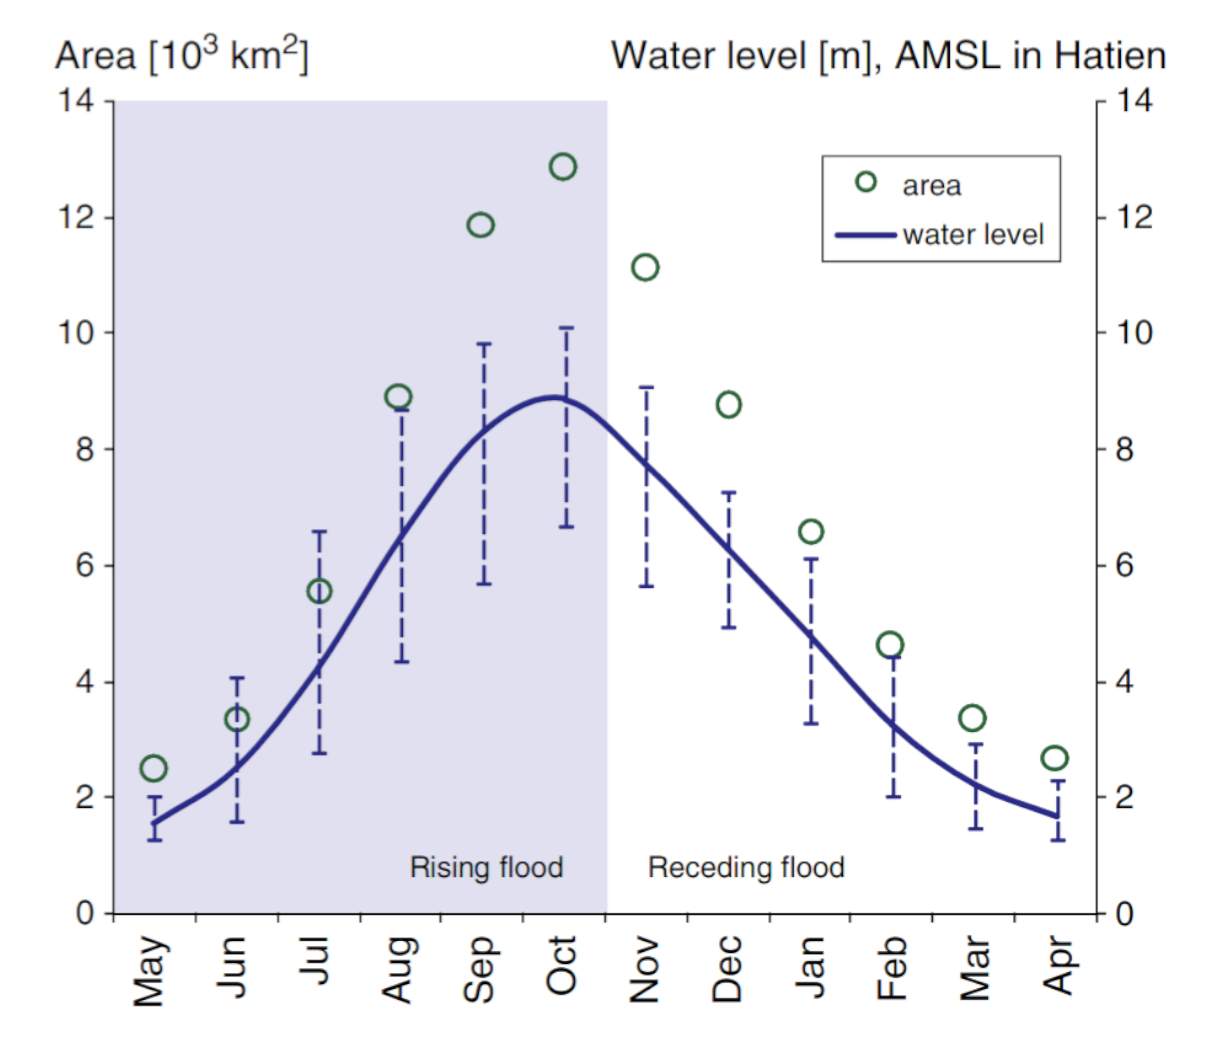
\includegraphics[width=.6\textwidth]{figures/chap4/tonlesap_avg_area_with_floodplain.png} \cite{article:Water-balance-analysis-TonleSap}
    \label{fig:chap4-tonlesap-avg-area}
\end{SCfigure}


\section{Conclusions}
We have developed a model that can predict the next MODIS NDVI band with a high focus on lake's water body. The model consists of a single neural network that takes a well-organized set of historical MODIS NDVI bands and is trained end-to-end under the supervisor of ConvLSTM and an attention mechanism. Our evaluation shows strong performances of our method (A-CLSTM-G32) compared to previous methods in classification metrics. One the other hand, one of the limitations of the model is that we still have low performances on regression metrics. In addition, whether this approach can be used in higher resolution satellite image, such as Landsat or Sentinel-1 data, is still a controversy and is also a potential research subject. 


\section{Supplementary}
\label{Supplementary}
In this section we describe in detail algorithms used for extracting lake's water body.

\begin{algorithm}
    \caption{mask\_lake\_img}
    \begin{algorithmic}[1]
        \Inputs{\begin{itemize}
                \item{$(X)$: Tensor with shape ($H,W$),}
                \item{$water\_threshold$: Double scalar which is threshold of pixel value to be considered as water.}
            \end{itemize}}
        \Outputs{$M$: 0-1 Tensor, with shape ($H,W$): Mask tensor, \\ \quad \quad 1 if the pixel is on lake boundary and 0 otherwise.}
        \newline
        \State $masks \gets$ classify\_by\_threshold($X$)
        \State{$labels \gets$ find\_connected\_elements($mask$)}
        \Returns{largest\_connected\_elements($labels$)}
    \end{algorithmic}
\end{algorithm}

\begin{algorithm}
    \caption{find\_boundary\_mask\_lake}
    \begin{algorithmic}[1]
        \Inputs{\begin{itemize}
            \item{$(X)$: Tensor with shape ($H,W$),}
            \item{$water\_threshold$: Double scalar which is threshold of pixel value to be considered as water.}
        \end{itemize}}
        \Outputs{$M$: 0-1 Tensor, with shape ($H,W$): Mask tensor,\\ \quad \quad if the pixel is on lake 1 if pixel is on lake boundary and 0 otherwise.}
        \newline        
        \State $X_1 \gets$ mask\_lake\_img($X, water\_threshold$)
        \Returns{find\_boundaries($X_1$)}
    \end{algorithmic}
\end{algorithm}


\chapter{Water level Prediction based on High-resolution Synthetic Aperture Radar Images}
\label{chap-5-predict-from-sar-image}
\begin{ChapAbstract}
In this chapter, we would like to apply machine learning approach, especially deep learning, to predict the water body in the next future. We apply an extension on Long Short-Term Memory (LSTM), Conv-LSTM, to tackle problem. Conv-LSTM layer is not only take advantage from previous state-of-the-art approach in this kind of problems, Fully-Connected LSTM, but also very suitable to spatial-temporal data due to inherent convolutional structure. Because the common information that we can accquired from water body and rainfall intensity, are spatial and temporal, we apply model from precipitation nowcasting problem to our prediction problem, modify about ways to train model, then Tri An Reservor is one more time selected to take experiment on. 

\end{ChapAbstract}

\section{Introduction}

% Time-series data prediction: Video / Precipitation Nowcasting.

Prediction (a.k.a. sequence prediction) is one of interesting fields in machine learning, in which the input (sequence data) contains an order on the observations and this order must be preserved while training model and making prediction.

\begin{figure}[h!]
	\centering
	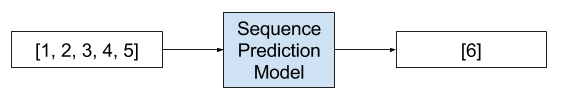
\includegraphics[width=0.7\textwidth]{figures/Example-of-a-Sequence-Prediction-Problem.png}
	\caption[]{Example of simple sequence prediction}
	\label{fig:exampleSimpleSequencePrediction}
\end{figure}

There are some example of sequence prediction problems, including:

\begin{enumerate}
	\item \textbf{Stock Market Prediction}\cite{Pagolu2016,Liu2018}. Given sequence of stock value as input, predict the expected next stock value. 
	
	\item \textbf{Product Recommendation}\cite{Wang2018,Cao2019}. Given sequence of recent purchased goods of a customer, predict the thing that the customer might "add to cart" next, and then make recommendation. 
	
	\item \textbf{Weather Forecasting}\cite{Quan2000,Wang2017}. Given sequence of weather observation over a period of time, predict the expected weather in next point of time.
	
\end{enumerate}

% Related to water body from satellite images, figure out why it related and its expansion: periodical information

One of important fields of weather forecasting is Nowcasting Precipitation\cite{Sun2013}. The goal of this task is about giving precise prediction of rainfall intensity in a region, over a short period of time. Recent advances in deep learning, Recurrent Neural Networks (RNNs), especially Long Short-Term Memories (LSTMs) models\cite{Graves2013GeneratingSW,Hochreiter1997,Cho2014,Donahue2017} provides good results on this kind of problem. In this chapter, we would like to predict the next water body shape (related to its area), from its time-series data. The common things between nowcasting precipitation and this problem is they both have spatial, spectral and temporal information inside data. We would like to apply model containing Conv-LSTM-2D layer\cite{Shi2015ConvolutionalLN}, to solve our proposed problem. Conv-LSTM-2D layer is recently used in computer vision, especially spatial-temporal problems. In this problem, we would like to extract the spatial feature as well as the correlation in the time. The fully-connected LSTMs can capture the temporal correlation but do not encode the spatial data. That's why they propose a model where the input to state and state to state transitions are convolutional. The model in \cite{Shi2015ConvolutionalLN} show better result on capturing spatial-temporal correlations than other state-of-the-art methods. So in this chapter, we will take this model as reference to provide solution for our problem, for Tri An reservoir.

\paragraph{Synthetic Aperture Radar (SAR) Images} \footnote{https://en.wikipedia.org/wiki/Synthetic-aperture\_radar} SAR is a form of radar, which mainly used to produce two or three-dimensional reconstructions of objects. SAR is motivated for high-resolution remote sensing and it is independent of weather. It also has many application in remote sensing, including topography, oceanography; environment monitoring such as oil spills, flooding, urban growth, global change and military surveillance and so on. 

\begin{figure}[h!]
	\centering
	\includegraphics[width=0.4\textwidth]{figures/TEIDE.jpg}
	\caption[]{Teide volcano on the island of Tenerife in the Canary Islands, Spaceborne Imaging Radar-C/X-Band Synthetic Aperture Radar.}
\end{figure}

\paragraph{Sentinel 1-A Satellites} The Sentinel-1 mission \footnote{https://sentinel.esa.int/web/sentinel/missions/sentinel-1} comprises a constellation of two polar-orbiting satellites, operating day and night, in order to acquire imagery regardless of the weather. This is one of big benefits when comparing with Landsat satellites. Launched on 3rd April 2014, Sentinel-1A is placed in a near-polar, sun-synchronous orbit with a 12-day repeat cycle and 175 orbits per cycle.

\section{Dataset} 

In this chapter, Tri An reservoir is chosen for experiments. Because Radar Satellites Images is not affected by cloud cover like optical satellite in \ref{chap-3-recover-water-body}, so we only focus on prediction water body. The SAR images monthly imagery provided from Sentinel-1 satellites are collected from \textit{November 25tr, 2015} to \textit{June 1st, 2019} for training and evaluating. 

Depending on coordinates of Tri An Reservoir, the original image has been cropped to size \textit{2560 px} x \textit{3840 px}, enough to show its water body.

\paragraph{Water body segmentation on Sentinel-1 Image} In this chapter, in order to segment out water body, we depend on \textbf{V}ertical Transmit-\textbf{H}orizontal Receive Polarization (VH) or \textbf{V}ertical Transmit-\textbf{V}ertical Receive Polarization (VV), and apply corresponding threshold:

\begin{equation}
\centering
VH \leq -21
\end{equation} 

\begin{equation}
\centering
VV \leq -17
\end{equation} 

\subparagraph{Polarization} Polarization is a way to give transmission signals a specific direction. It makes the beam more concentrated. Signals transmitted by satellite can be polarized in one of four different ways: linear (horizontal or vertical) or circular (left-hand or right-hand). To use the channels that are available for satellite broadcast as efficiently as possible, both horizontal and vertical polarization (and left- and right-hand circular polarization) can be applied simultaneously per channel or frequency. Horizontal and vertical transmissions will therefore not interfere with each another because they are differently polarized. This means twice as many programs can be transmitted per satellite. Consequently, via one and (almost) the same frequency the satellite can broadcast both a horizontal and a vertical polarized signal (H and V), or a left- and right-hand circular polarized signal (LH and RH).

\begin{itemize}
    \item \textbf{\textit{V}ertical Transmit-\textit{H}orizontal Receive Polarization (VH)} is a mode of radar polarization where the microwaves of the electric field are oriented in the vertical plane for signal transmission, and where the horizontally polarised electric field of the backscattered energy is received by the radar antenna.
    \item \textbf{\textit{V}ertical Transmit-\textit{V}ertical Receive Polarization (VV)} is a mode of radar polarization where the microwaves of the electric field are oriented in the vertical plane for both signal transmission and reception by means of a radar antenna. In this case, the plane of the electric field of the microwave energy is designated by the letter V (vertical) for both transmit and receive events, i.e. VV; this transmit-receive polarity is also called like-polarised as opposed to cross-polarised (horizontal transmit - vertical receive, HV). 
\end{itemize}

Because in our cropped image that only contains Tri An Reservoir as the largest water body, so we only need to find out the most largest one, using Bread-First Search algorithm\footnote{https://en.wikipedia.org/wiki/Breadth-first\_search}. With this object, we easily to figure out the boundaries, with help of function \textit{find\_boundaries}, from Python library \textit{Scikit-Image}\footnote{https://scikit-image.org/}.

% \pagebreak
\section{Model}

In this thesis, we stack Encoding-Forecasting Conv-LSTM layer to for building prediction model. Our input and output of model are all 3D tensors, size of $T x W x H$, in which $T = 12$ for temporal information (12 consecutive months), where $W x H$ is size of each data point image for spatial information. This helps our model preserve all spatial and temporal information, so that, it can tackle the complex water body prediction problem, with multiple stacked of Conv-LSTM-2D. In Figure \ref{fig:structureConvLSTM2D}, the encoding LSTM compresses, while the whole input sequence into a hidden state tensor and the forecasting LSTM unfolds this hidden state to give the final prediction.

\begin{figure}[h!]
	\centering
	\includegraphics[width=0.8\textwidth]{figures/convlstm_sample.PNG}
	\caption[]{Structure of Encoding-Forecasting Conv-LSTM network in \cite{Shi2015ConvolutionalLN}}
	\label{fig:structureConvLSTM2D}
\end{figure}

Conv-LSTM-2D is already provided in Keras framework\footnote{https://keras.io/layers/recurrent/}. Model structure is shown in Figure \ref{fig:timeModel}.

\begin{figure}[h!]
	\centering
	\includegraphics[width=0.4\textwidth]{figures/time_model.png}
	\caption[]{Prediction mode, based on Conv-LSTM-2D}
	\label{fig:timeModel}
\end{figure}

Specification:

\begin{itemize}
	\item \textit{Input and Output} Because we only focus on predicting water body, so after extracting water body from original image and finding out its boundaries, we randomize on boundaries 50 tiles with size of 128 x 128. There is 12 consecutive images, corresponding to 12 month in year. The output is a image of next month, which is same month of 1st image in input sequence but next year. 
	
	\item \textit{Conv3D} This type of layer helps to catch spatial and temporal invariances in the same manner as \textit{Conv2D} in an imagery case. This make the curse of dimensionality much less harmful. Because at the end of model, we need to have a prediction, so it's no longer to keep temporal information after this layer.
	
	\item \textit{Batch Normalization} Batch normalization reduces the amount by what the hidden unit values shift around (covariance shift). Morever, this layer allows each layer of a network to learn by itself a little bit more independently of other layers.
	
	\item \textit{Activation} The activation for Conv-LSTM-2D is $tanh$ function, for Conv3D is $sigmoid$ function.
	
	\item \textit{Dropout and Recurrent Dropout} In Recurrent Neural Networks, we have two definition about \textbf{Dropout} and \textbf{Recurrent Dropout}. \textbf{Dropout} describes fraction of the units to drop for the linear transformation of the inputs, while \textbf{Recurrent Dropout} show fraction of the units to drop for the linear transformation of the recurrent state (more detail at \cite{Gal2015}). In this model, with each Conv-LSTM-2D layer's configuration, $dropout$ is set at $0.4$, and and $recurrent\_dropout$ is $0.3$.
	
	\item \textit{Model compilation parameters} Like model compilation in \ref{chap-3-recover-water-body}, the loss function is still $mean\_square\_error$, optimizer is $adam$ and evaluation metric is $PSNR$(\ref{psnr_eq}). 
	
\end{itemize}

\section{Experiments}

\subsection{Prediction water body area}

The time-series data in one year (one file per month) has been divided into tile of \textit{128 px } x \textit{128 px}. All tiles belong to wate body are predicted but only area and boundaries of water body are evaluated. Figure \ref{fig:inputTs} show the sample input from June 2018 to May 2019, and the groundtruth of the next point of time, which is retrieved in June 2019, is shown at Figure \ref{fig:outputTs}. \textit{Note that, the yellow squares show example splited tile for prediction model. They are zoomed out in Figure \ref{fig:tileInputTs}}.

\begin{figure}[h!]
	\begin{center}
        \begin{tabular}[b]{c}
            \includegraphics[width=0.3\linewidth]{figures/inputDemo_chap5/06.jpg}
        \end{tabular}
        \begin{tabular}[b]{c}
            \includegraphics[width=0.3\linewidth]{figures/inputDemo_chap5/07.jpg}
        \end{tabular}
        \begin{tabular}[b]{c}
            \includegraphics[width=0.3\linewidth]{figures/inputDemo_chap5/08.jpg}
		\end{tabular}
        \begin{tabular}[b]{c}
            \includegraphics[width=0.3\linewidth]{figures/inputDemo_chap5/09.jpg}
        \end{tabular}
        \begin{tabular}[b]{c}
            \includegraphics[width=0.3\linewidth]{figures/inputDemo_chap5/10.jpg}
        \end{tabular}
        \begin{tabular}[b]{c}
            \includegraphics[width=0.3\linewidth]{figures/inputDemo_chap5/11.jpg}
		\end{tabular}
        \begin{tabular}[b]{c}
            \includegraphics[width=0.3\linewidth]{figures/inputDemo_chap5/12.jpg}
        \end{tabular}
        \begin{tabular}[b]{c}
            \includegraphics[width=0.3\linewidth]{figures/inputDemo_chap5/01.jpg}
        \end{tabular}
        \begin{tabular}[b]{c}
            \includegraphics[width=0.3\linewidth]{figures/inputDemo_chap5/02.jpg}
		\end{tabular}
        \begin{tabular}[b]{c}
            \includegraphics[width=0.3\linewidth]{figures/inputDemo_chap5/03.jpg}
        \end{tabular}
        \begin{tabular}[b]{c}
            \includegraphics[width=0.3\linewidth]{figures/inputDemo_chap5/04.jpg}
        \end{tabular}
        \begin{tabular}[b]{c}
            \includegraphics[width=0.3\linewidth]{figures/inputDemo_chap5/05.jpg}
		\end{tabular} 
    \end{center}
	\caption[]{Sample input. From left to right, top to bottom: Time-series sequence from June 2018 to May 2019.}
	\label{fig:inputTs}
\end{figure}

\begin{figure}[h!]
	\centering
	\includegraphics[width=1\textwidth]{figures/tileInput.png}
	\caption[]{Input as tile to model, cropped from original in Figure \ref{fig:inputTs}}
	\label{fig:tileInputTs}
\end{figure}

The groundtruth output from above input is shown at Figure \ref{fig:outputTs}.

\begin{figure}[h!]
	\centering
	\includegraphics[width=1\textwidth]{figures/output_ts.png}
	\caption[]{Sample output: Groundtruth of water body in next time of sequence, June 2019.}
	\label{fig:outputTs}
\end{figure}

The prediction result of model, from Feb 2019 to June 2019 is shown in table \ref{table:predictValue}.

% Show table, contains result

\begin{table}[h!]
	\centering
	\begin{tabularx}{\textwidth}{|Y|Y|Y|Y|Y|}
		\hline
		\textbf{Month} & \textbf{Groundtruth Area ($km^2$)} & \textbf{Predicted Area ($km^2$)} & \textbf{True Prediction Ratio (\%)} & \textbf{False Prediction Ratio (\%)}\\ \hline
		2              & 282.5946                                          & 287.7469                                        & 98.32 & 3.44                         \\ \hline
		3              & 296.5101                                          & 301.0503                                        & 97.02 & 
		4.44                          \\ \hline
		4              & 301.2402                                          & 276.8264                                        & 87.60 & 4.68                         \\ \hline
		5              & 273.7712                                          & 273.0462                                        & 96.39 & 3.35                          \\ \hline
		6              & 243.2829                                          & 217.7548                                        & 86.40 & 3.47                         \\ \hline
	\end{tabularx}
	\caption[]{Area prediction result and ratio}
	\label{table:predictValue}
\end{table}

% Plot predicted result, with groundtruth value

\begin{figure}[h!]
	\centering
	\includegraphics[width=1\textwidth]{figures/comparePredict.png}
	\caption[]{Area comparison between groundtruth and prediction.}
	\label{fig:comparePredict}
\end{figure}

Figure \ref{fig:prediction_02}, \ref{fig:prediction_03}, \ref{fig:prediction_04}, \ref{fig:prediction_05} and \ref{fig:prediction_06} are groundtruth and corresponding prediction for Tri An Reservoir water body from 12 previous months, from February to June 2019, in which the yellow line shows boundaries of predicted water body.

% Show 2-6/19 prediction, with result and boundaries.
\begin{figure}[h!]
	\centering
	\includegraphics[width=0.9\textwidth]{figures/20190202T110307.png}
	\caption[]{Prediction, Feb 2019}
	\label{fig:prediction_02}
\end{figure}

\begin{figure}[h!]
	\centering
	\includegraphics[width=0.9\textwidth]{figures/20190309T223707.png}
	\caption[]{Prediction, March 2019}
		\label{fig:prediction_03}
\end{figure}

\begin{figure}[h!]
	\centering
	\includegraphics[width=0.9\textwidth]{figures/20190402T223708.png}
	\caption[]{Prediction, April 2019}
		\label{fig:prediction_04}
\end{figure}

\begin{figure}[h!]
	\centering
	\includegraphics[width=0.9\textwidth]{figures/20190508T223709.png}
	\caption[]{Prediction, May 2019}
		\label{fig:prediction_05}
\end{figure}

\begin{figure}[h!]
	\centering
	\includegraphics[width=0.9\textwidth]{figures/20190601T223710.png}
	\caption[]{Prediction, June 2019}
		\label{fig:prediction_06}
\end{figure}


\subsection{Example with anomaly detection}
\label{section:anomalyDetection}

One usage of sequence prediction output is about anomaly detection. This problem is usually formulated as finding outlier data points, relative to some standard or usual signal. In this chapter, the data points show water body area of Tri An Reservoir. The below chart show observations of Tri An reservoir area in 3 years, from 2016-2018.

\begin{figure}[h!]
	\centering
	\includegraphics[width=0.9\textwidth]{figures/observations.png}
	\caption[]{Observations of Tri An reservoir from Sentinel-1 Satellite, in term of water body area. Notice that, on July 2017, the water body area is seemed to be different from year 2016 and 2018}
	\label{fig:observation}
\end{figure}

Following observations, the groundtruth area of water body in 2016, 2017 and 2018 are $189.6926 km^2$, $242.4104 km^2$ and $178.4857 km^2$ respectively. While using our model, the prediction is approximately $189.6926 km^2$. See more about visualization at Fig. \ref{fig:anomalyVis} and graph for comparison at Fig. \ref{fig:anomalyComp}

\begin{figure}[h!]
	\centering
	\includegraphics[width=0.9\textwidth]{figures/20170706T110259.png}
	\caption[]{Prediction for July 2017, using 12 previous data points (from July 2016 to Jun 2017)}
	\label{fig:anomalyVis}
\end{figure}


\begin{figure}[h!]
	\centering
	\includegraphics[width=0.9\textwidth]{figures/anomaly.png}
	\caption[]{Prediction (the red point) and groundtruth (the green line) on July 2017}
	\label{fig:anomalyComp}
\end{figure}

\section{Conclusions}

In this chapter, we have an acceptable result on applying deep learning to prediction problem on Tri An Reservoir, in term of water body area and its boundaries. This potential result may help us a lot when dealing with sequence prediction problem, especially complicated situation, such as spatial-temporal sequence forecasting problem, using proposed extension of LSTM - Conv-LSTM-2D. Beside that, with accepted prediction, the output of this problem may be used on other sequence problems, such as anomaly detection that we've taken example in \ref{section:anomalyDetection}. For future work, when enough data for training and testing, an end-to-end real-time forecasting water body observer system might be proposed, with two main parts: Prediction part and classification for anomalies part. 
\chapter{Conclusions and Future Works}
\label{chap-6-conclusions}
\begin{ChapAbstract}
In this chapter we would like to summary what we've done in this thesis, with potential result when applying solution from sequence prediction into solving some interesting remote sensing problems, including water body recovery and water body area prediction over the time. Then finally, some of future works are provided.
\end{ChapAbstract}

\section{Conclusion}

We've almost done on bringing in data at scale and machine learning techniques with the goal of experimenting and designing end-to-end models to solve:

\begin{enumerate}
	\item \textbf{Landsat clouds covered image recovery} With Landsat satellites, it is not enough data for whole cycle of water body in a year, but the \textbf{trend} of water body in few recent months might feed temporal information into our modified model from STS-CNN method. The result of chapter \ref{chap-3-recover-water-body} might be better if the input is directly cropped on water body boundaries, without resizing or stretching. Recovery model with continous data as reference should be more strictly trained, even if two main parts (prediction model in order to predict next image as reference and recovery model) are pre-trained separately, because of each difficulties.
	
	\item \textbf{Making Prediction with MODIS and Sentinel-1 Data} The data is more abundant that we could build up a dataset which contains full cycle of water body information in a whole year. This temporal attribute is very useful for prediction model to predict the water body in the near future. SAR-image from Sentinel-1 satellite has many benefits, not only being unaffected from cloud cover like optical satellites imagery, but also provide depth information of water body. Combining with area, the follow-up remote sensing problem might be solved: \textbf{Water body volume prediction}.
\end{enumerate}

Three main Chapter \ref{chap-3-recover-water-body}, \ref{chap-4-predict-water-body} and \ref{chap-5-predict-from-sar-image} show potential results when applying time-series data to extract and feed temporal information into deep learning models, to solve different remote sensing problems. Each kind of satellites has many different advantages and disadvantages. In the time we're completing this thesis, we have also learnt how to deal with each type of remote sensing imagery. Landsat data used in Chapter \ref{chap-3-recover-water-body} have an adequately high resolution, however their temporal frequency are quite sparse, which makes them hard to be applied as a sole source of data. In constrast, MODIS data used in Chapter \ref{chap-4-predict-water-body} have a higher temporal frequency, but their quality is usually not well-quality enough due to the low resolution and the high cloud pixel rate problem. Sentinel-1 data have an impressive resolution, however they have just been released since 2014, which prevents them to be directly applied in real world deep learning projects. In conclusion, the complete research on all of these three types of remote sensing data is so necessary with regard to everyone who wants to adopt these useful source of data to solve a real world problem.  

\section{Future works}

In this thesis, the main purpose we would like to aim, is about sequentially predicting the pixels in an image along the two spatial dimensions. There are other methods that discrete probability of the raw pixel values and encodes the complete set of dependencies in the image: PixelCNN \cite{OordKK16} and its improved version, PixelRNN\cite{OordKVEGK16}. These solutions might not only give considerable results, but also speed up the training time/evaluation time, to predict the next water body for consecutive images.

Our works show that an end-to-end models can solve some different problems in remote sensing. Climate change, reservoirs, hydro power-plants, and irrigation systems have been identified as major factors which are redefining hydrological cycles in agricultural areas. In the Greater Mekong subregion, the home of more than 300 million people, the trend is increasing and visibly recognized year after year. Being the country at the end of the Mekong River, Vietnam has been enjoying numerous advantages from the river for centuries. but now is facing big threats of droughts and unpredictable floods. Causes have been named to a large number of reservoirs and hydro power-plant being built along the river, spreading from Laos, Thailand, and Cambodia. A big external factor is giant reservoirs in Tibet, China, where the river starts. A more idea is observation of inter-connected rivers, lakes, reservoirs in many different countries to manage whole large area of Mekong river here, as water body is not affected by itself, but also by weather, amount of rain and many different tributaries. For example, there are many different rivers that have flown into the Mekong river: Menam Mun River (Thailand), Xe Don (Laos) or Tonlé San (Cambodia). 

Served as an exemplar, once hydrological events are becoming predictable in the Greater Mekong subregion, it can be applied to many other agricultural areas in the world. If following up this idea and expanding it, we will be able to design a system which can monitor and predict hydrological disasters ahead of time, facilitating appropriate reaction time for farmers and governments. The abundance of remote sensing data with free cost from NASA and ESA has giving us a big advantage in tacking this problem. With a long operational time since before 1980, satellite programs such as MODIS and Landsat have generated precious historical Earth Observatory data. Moreover, as the Corpernicus program from ESA with a series of Sentinel satellites, including optical and radar instruments, has been launched since 2014, the project is just in the right time for being solved.

%%%%%%%%%%%%%%%%%%%%%%%%%%%%%%%%%%%%%%%%%%%%%%%%%%%%%%%
% The bibliography. Turn on page numbering.
%%%%%%%%%%%%%%%%%%%%%%%%%%%%%%%%%%%%%%%%%%%%%%%%%%%%%%%
\addtocontents{toc}{\protect\cftpagenumberson{chap}}
%%%% Soooo if IPS says there should be 5cm top margin
%%%% on the ``References'' heading page, uncomment the
%%%% line just before and after \bibliography. Repeat for
%%%% \bibliographyown if necessary
%% Increase spacing before chapter heading
\titlespacing*{\chapter}{0pt}{\dimexpr2.5cm-50pt}{\baselineskip}
\bibliography{refs}
% \bibliographystyle{plain}
% now change it back to normal
\titlespacing*{\chapter}{0pt}{-50pt}{\baselineskip}

\assignpagestyle{\chapter}{plain}

%%%%%%%%%%%%%%%%%%%%%%%%%%%%%%%%%%%%%%%%%%%%%%%%%%%%%%%
% The list of own publications.  If you don't have one, you may
% comment out the next 4 lines.
%%%%%%%%%%%%%%%%%%%%%%%%%%%%%%%%%%%%%%%%%%%%%%%%%%%%%%%
% Uncomment/comment this line if you need the List of Publications to be bold/not bold in the ToC.
\addtocontents{toc}{\protect\renewcommand\protect\cftchapfont{\protect\bfseries}}
\nociteown{3dor.20181052}
\bibliographyown{mybib}

\end{document}